\documentclass[a4paper, 12pt, oneside, polutonikogreek, english]{article}
\usepackage[utf8]{inputenc}
\usepackage{fouriernc}
\usepackage{csquotes}
\usepackage{booktabs}
\usepackage{url}
\usepackage{graphicx}
\setlength{\emergencystretch}{15pt}
\graphicspath{ {./figures/} }
\usepackage[figurename=]{caption}
\usepackage{fancyhdr}
\usepackage{amssymb}
\usepackage{array}
\usepackage{float}
\usepackage{imakeidx}
\usepackage{qtree}
\usepackage{microtype}
\usepackage{textalpha}
\usepackage{wasysym}
\usepackage{cjhebrew}
\usepackage{pdflscape}
\usepackage{longtable}
\renewcommand{\listfigurename}{List of Plates}
\makeindex[columns=2, title=Alphabetical Index, intoc]

\usepackage[dvipsnames]{xcolor}
\usepackage{eso-pic,graphicx}
\usepackage[top=40mm, bottom=54mm, outer=47mm, inner=47mm]{geometry}
\setlength{\columnsep}{90pt}

\definecolor{customColor}{RGB}{255, 224, 132}

\usepackage{sectsty}
\usepackage[titles]{tocloft}

\usepackage{setspace}
\onehalfspacing

% change color of text, example replace all \color{Goldenrod} with \color{lightgray}

\makeatletter % change only the display of \thepage, but not \thepage itself:
\patchcmd{\ps@plain}{\thepage}{\bfseries\color{customColor}{\thepage}}{}{}

\makeatother

\color{customColor}
\begin{document}
\bfseries
\renewcommand{\thefootnote}{{\color{customColor}\bfseries\tiny\arabic{footnote}}}
\let\oldfootnote\footnote
    \renewcommand{\footnote}[1]{\oldfootnote{\color{customColor}\bfseries\footnotesize#1}}
\AddToShipoutPictureBG{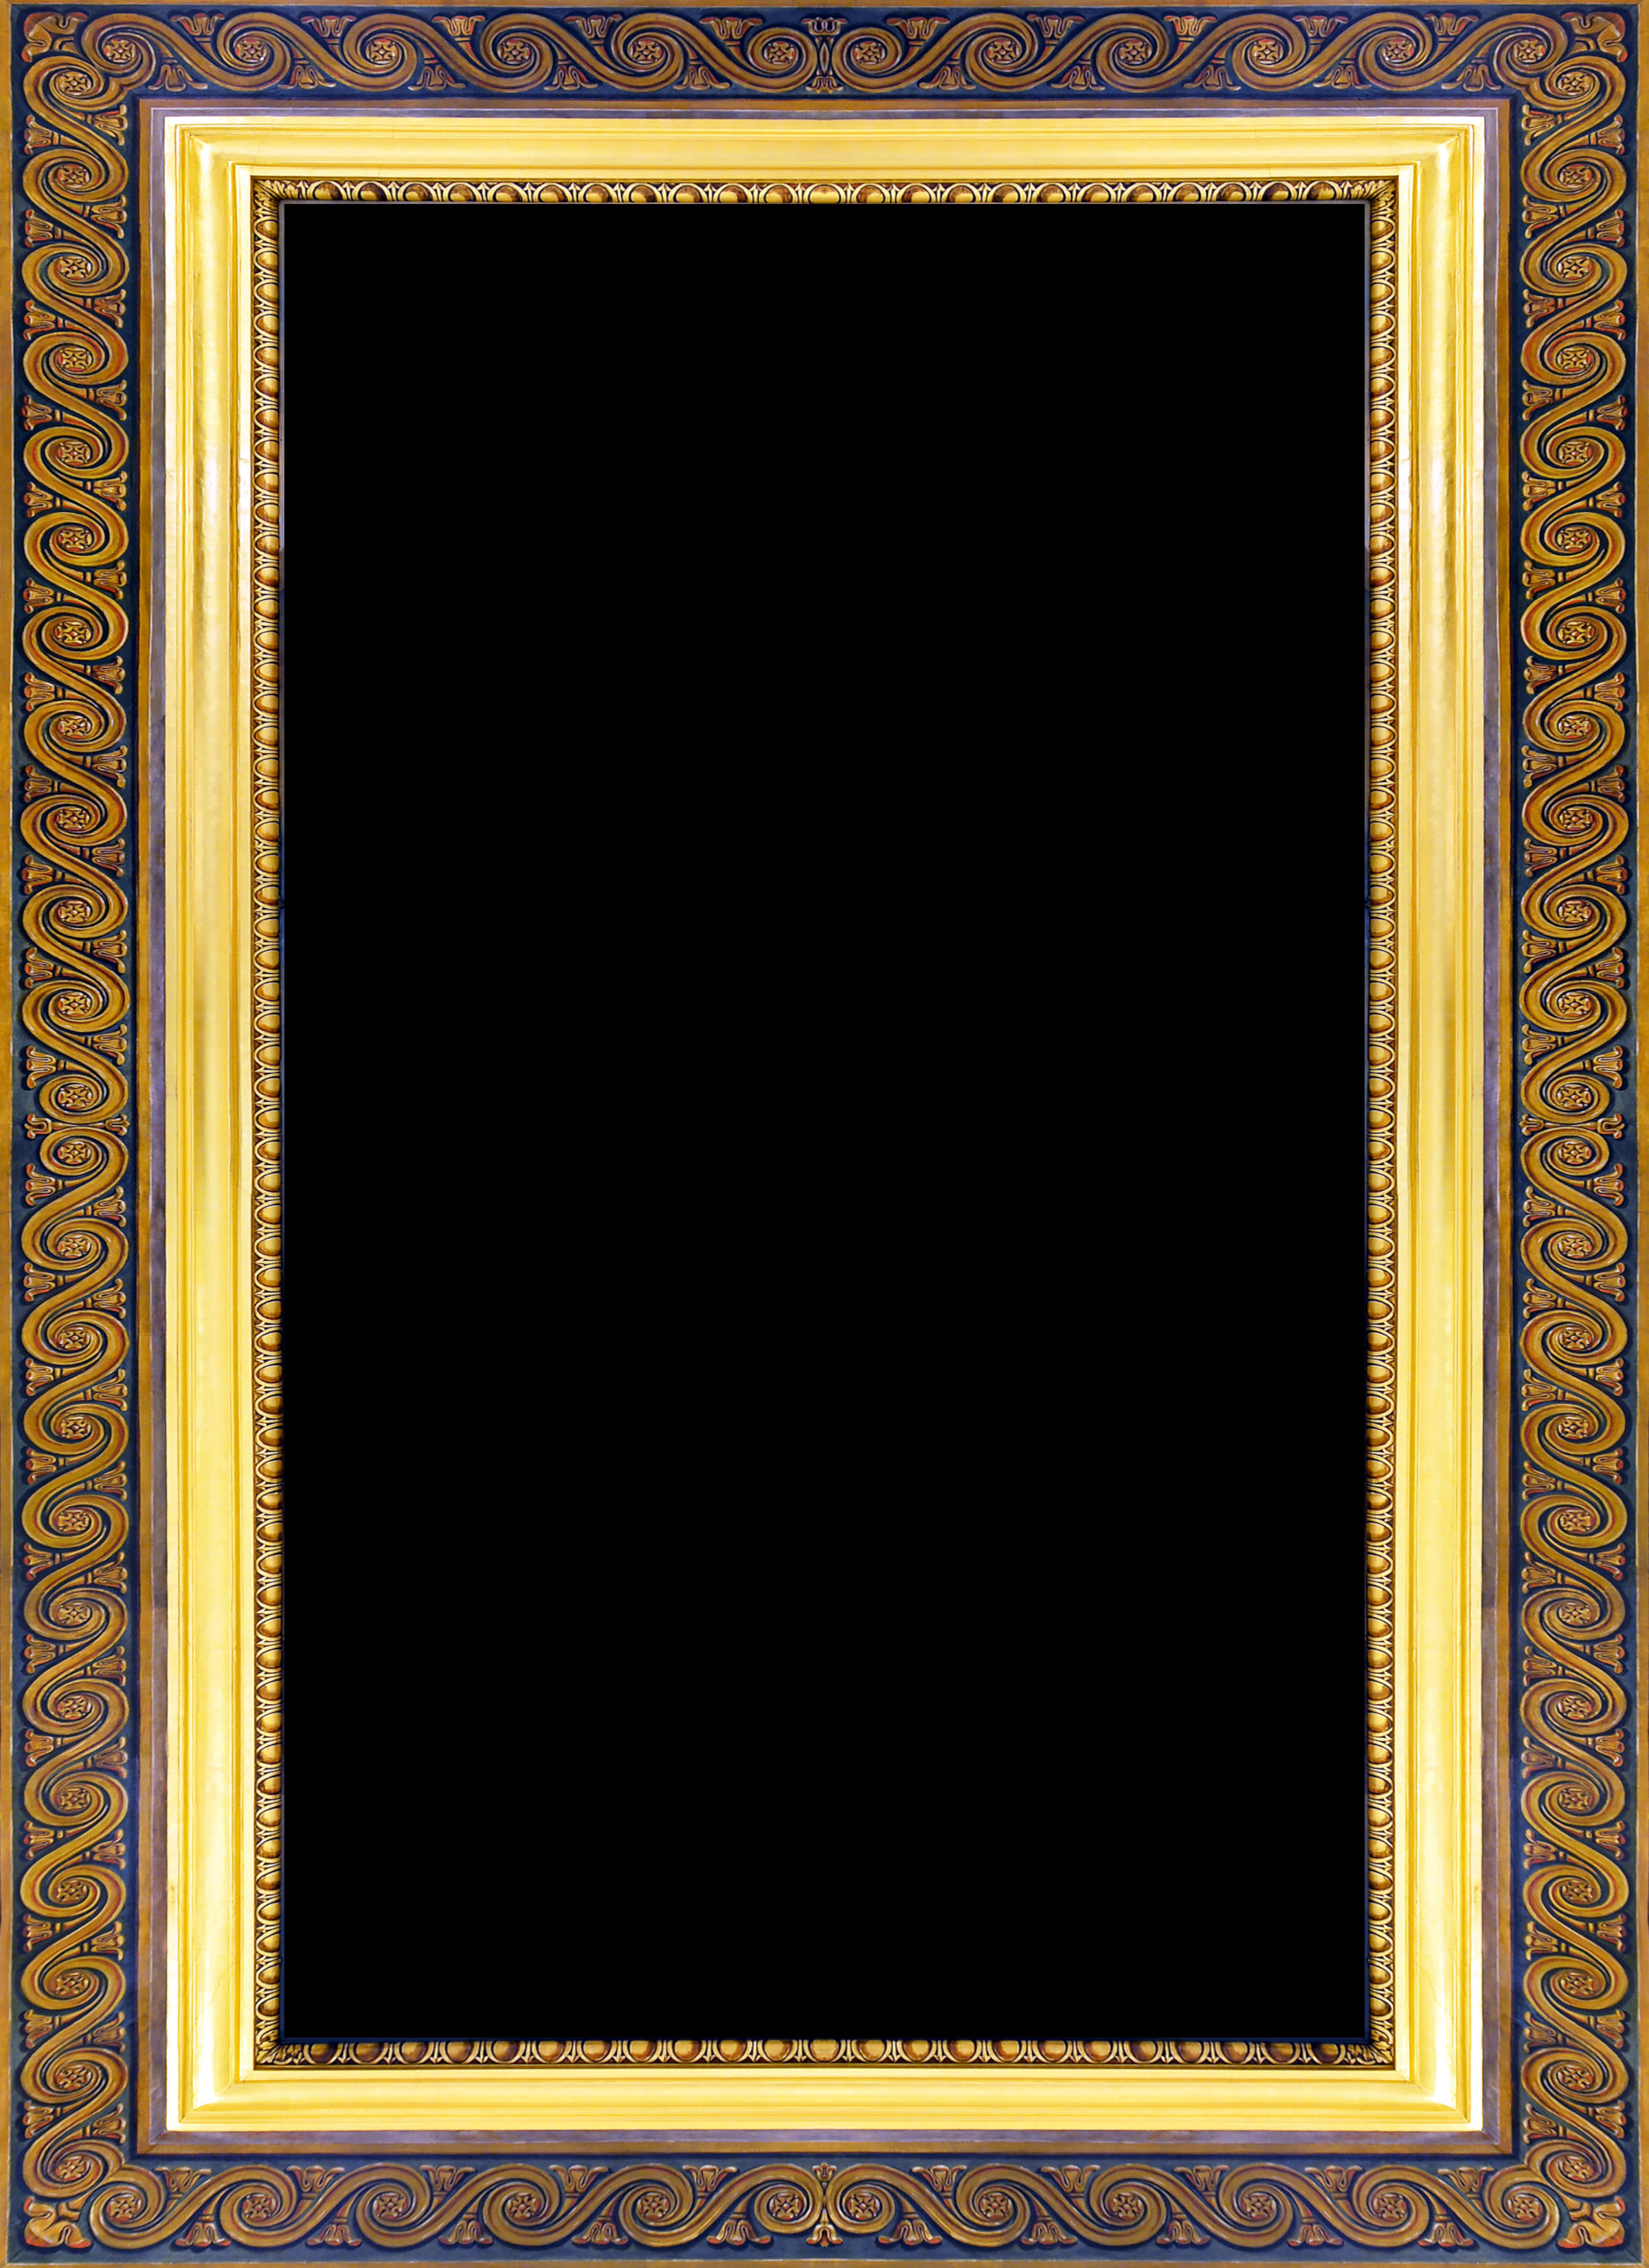
\includegraphics[width=\paperwidth,height=\paperheight]{border4.jpeg}}
\begin{titlepage} % Suppresses headers and footers on the title page
	\centering % Centre everything on the title page
	\scshape % Use small caps for all text on the title page

	%------------------------------------------------
	%	Title
	%------------------------------------------------
	
	\rule{\textwidth}{1.6pt}\vspace*{-\baselineskip}\vspace*{2pt} % Thick horizontal rule
	\rule{\textwidth}{0.4pt} % Thin horizontal rule
	
	\vspace{0.75\baselineskip} % Whitespace above the title
	
	{\Huge The Meteoritic Hypothesis} % Title
	
	\vspace{0.75\baselineskip} % Whitespace below the title
	
	\rule{\textwidth}{0.4pt}\vspace*{-\baselineskip}\vspace{3.2pt} % Thin horizontal rule
	\rule{\textwidth}{1.6pt} % Thick horizontal rule
	
	\vspace{1\baselineskip} % Whitespace after the title block
	
	%------------------------------------------------
	%	Subtitle
	%------------------------------------------------
	
	{A Statement on the Results of a Spectroscopic Inquiry into the Origin of Cosmical Systems} % Subtitle or further description
	
	\vspace*{1\baselineskip} % Whitespace under the subtitle
	
	%------------------------------------------------
	%	Editor(s)
	%------------------------------------------------

        {By Joseph Norman Lockyer, F. R. S.}
 
	\vspace{1\baselineskip} % Whitespace before the editors

        {\scriptsize Correspondant of the Institute of France; The Society for the Promotion of National Industry of France; The Royal Academy of Science, Göttingen; The Franklin Institute, Philadelphia; The Royal Medical Society of Brussels; Societa Spettroscopisti Italiani; The Royal Academy of Palermo; and Natural History Society of Geneva; Member of the Royal Academy of Lyncei, Rome; and the American Philosophical Society, Philadelphia; Honorary Member of the Academy of Natural Science of Cantania, Philosophical Society of York, Literary and Philosophical Society of Manchester, and Lehigh University; Member of the Committee on Solar Physics; Professor of Astronomical Physics in the Normal School of Science}
        
    %------------------------------------------------
	%	Cover photo
	%------------------------------------------------
	
	%\includegraphics[scale=1]{cover}
	
	%------------------------------------------------
	%	Publisher
	%------------------------------------------------
		
	\vspace*{\fill}% Whitespace under the publisher logo
	
	London and New York, 1890 % Publication year
	
	{\small MacMillan and Co.} % Publisher

	\vspace{1\baselineskip} % Whitespace under the publisher logo

        Internet Archive Online Edition  % Publication year
	
	{\small Attribution NonCommercial ShareAlike 4.0 International } % Publisher
\end{titlepage}
\setlength{\parskip}{1mm plus1mm minus1mm}
\setcounter{tocdepth}{3}
\setcounter{secnumdepth}{3}
\tableofcontents
\clearpage
\listoffigures{}
\clearpage
\begin{figure}[H]
\centering
\includegraphics[width=0.85\textwidth,keepaspectratio]{images-invert/Fig-Frontpage.png}
\caption*{\small \textsc{Frontispiece. --- The Chief Stars in the Pleiades.}}

\centerline{\small Photographed by Mr. Roberts, F. R. S., December 8, 1888.}
\end{figure}
\clearpage
\section*{Preface}
\paragraph{}
This volume has for its object the bringing together and coordinating of the observations which have been made up to the present time on the spectra of the various orders of cosmical bodies, in connection with laboratory work on which I have been engaged since 1868. It embodies in a connected form, among other matters, various Reports presented by me to the Solar Physics Committee, and subsequently communicated to the Royal Society; the President of the latter body having given me permission to utilise them as I have done in the present publication.

The work now considered follows logically upon researches which suggested that many solar phenomena might owe their origin to the falls of meteoritic masses upon the sun's surface. This subject I dealt with in a former book, \emph{The Chemistry of the Sun}, published in 1887, to which, in fact, the present volume is the natural sequel.

Since the book has been in type, advances have been made in several of the lines of inquiry touched upon --- the photographic study of nebular spectra may be cited as an instance --- which I should have gladly included; but as no new point of theoretical importance has been raised, I have thought it better not to delay publication in order to treat them in detail.

It may be that I should have added a final chapter, giving an account of the objections raised to the views here expressed. I have not done this because such objections as have been formulated have dealt only with small details of no fundamental importance for the hypothesis as a whole; and because, so far, it has been difficult for anyone to deal with the hypothesis in its generality, in consequence of the number of separate memoirs in which the results obtained from time to time have been published.

It is not in the nature of things that a large mass of detailed work and inquiry which has taken my assistants and myself three years to get together shall be found free from error, especially since observations made by many men in many lands, frequently under conditions of great difficulty, form part of the basis of the discussion. Nor, again, is it likely or even desirable that the general hypothesis, if it be found of any value at all, shall not be improved when fresh minds are brought to bear upon it.

When the time arrives, I shall profit more than anyone else by any valid objections that may be raised, and I shall be careful to reply to or accept them.

As the work proceeded many crucial tests were found, \emph{e. g.} in the so-called continuous spectrum of some nebulæ, the spectra of bright-line stars, and the differentiation of stars of Vogel's Class 2a into two groups, for which a telescope of large aperture was essential. In the body of the work I express my obligations to Mr. Common, F. R. S., and the Brothers Henry, of the Paris Observatory, for the assistance they have rendered in enabling me to apply the tests in question.

My thanks are due in this place to Professor A. S. Herschel, F. R. S., who permitted me to consult him on the early portions of the book dealing with luminous meteors, and was kind enough to look over the proofs; and also to Mr. Knott, who has freely permitted me to draw on his knowledge of the phenomena of variable stars.

I must also express my obligations to Mr. Roberts for generously permitting me to reproduce some of his marvellous photographs of nebulæ, and to Professor Pickering for forwarding to me some of the equally wonderful photographs of stellar spectra, which worthily form the basis of the Draper Memorial.

Among the assistants, on whose skill and industry I have relied for carrying out the details of the various investigations and the general reductions of observations, I must first mention Mr. Fowler, the Demonstrator of Astronomical Physics in the Normal School, whose aid has been quite invaluable, and whose keen interest in the work has never flagged. To Messrs. Taylor and Gregory I have chiefly looked for bringing together the work done at other observatories which has been discussed in this volume. Different branches of the laboratory and observatory work have fallen at different times upon Messrs. Atkins, Spencer, Porter, Baxandall, Coppen, and Sergeant Kearney, R. E.

J. Norman Lockyer.

\emph{6\textsuperscript{th} September} 1890.
\clearpage
\section{Part 1. The Fall and Nature of Meteorites.}
\subsection{Chapter 1. Ancient and Modern Records of Falls.}
\paragraph{}
Although Natural Science as a whole is a product of the modern world, this is by no means true of all branches of it; in some, by diving into the history of the past, we become acquainted with the phenomena which most forcibly impressed early man, and the effect produced by them on his mind.

Such an historical retrospect is of special interest in connection with the subject-matter of this book, for we learn from it that the falls of ``stones from heaven'' have been as constant in times past as in times present, and we are brought face to face with the stupendous awe inspired among whole peoples by what were considered to be omens coming visibly and directly from the Immortal Gods. The word omen really understates the old belief, for in many cases meteorites were placed in temples and regarded as the impersonations of the deities, even in Greece as well as in the East. In the temple of Aphrodite at Paphos and in that of Apollo at Delphi a conical stone stood in the place of an image; these were in all probability meteorites like the image at Ephesus, mentioned by St. Paul.

The earliest fall recorded in the annals of the Western world dates from 1478 B. C. It happened in Crete, but the record is much more doubtful than that of the falls in 705 and 654 B. C., noted, the first by Plutarch, and the second by Livy.

But it is agreed on all hands that the first fall to which the greatest interest attaches was observed in the Thracian Chersonesus, on the banks of the river Ægospotamos, 468 B. C. Aristotle, Plutarch, Pliny,\footnote{\emph{N. H.} vol. 2. p. 59.} and other ancient authors refer to the circumstances of the fall, which are also recorded in the Parian chronicle engraved on marble, which is now one of the glories of the University Galleries at Oxford.\footnote{I learn from Professors Pritchard and Gardner that the upper half of the marble slab disappeared at Arundel House many years ago. The remaining part is so damaged by weather and probably by fire that no intelligible photograph of any part of it could be taken. A transcription of the marble, made when it was far better preserved, is given in Boeckh's \emph{Corpus Inscriptionum Græcorum}, vol. 2. p. 293, 2374.} This meteorite was as large as two millstones. It is noteworthy that in connection with it Anaxagoras was accused of having predicted the fall of this and others from the sun, which he regarded as a molten fiery mass.\footnote{\emph{Cosmos}, Otté's translation, vol. 1. p. 110.}

Whatever its origin, it was held in veneration by the Thracians, and the subsequent defeat of the Athenians in the neighbourhood was attributed to its virtues. Humboldt relates that the African traveller Brown made a journey to Thrace to find it, but without success.

M. Daubrée, in his volume on the \emph{Interior of the Earth},\footnote{\emph{Régions invisibles du Globe et des Espaces célestes}, International Scientific Series, p. 150.} has collected together much interesting information relating to the next great historic fall --- that at Pessinuntia in Phrygia in 264 B. C. This became the object of a special cult --- that of Cybele, the mother of the gods. The Decemviri, charged with the custody of the Sibylline leaves, declared that the presence of the stone would bring about the expulsion of the Carthaginians from Italy, and with the consent of Attala it was brought to Rome with splendid pomp, which clearly indicates to us how firmly its divine nature and origin were believed in. The oracle of Delphi, on being consulted, declared that the most honest man should take charge of it. The Senate having declared that Scipio Nasica was that man, he proceeded to Ostia amidst general rejoicing and accompanied by a train of noble Roman ladies, who in turn bore it back to its appointed resting-place, the Temple of Victory. The stone itself was small and black, and had been mounted in silver; the visible part bore a resemblance to a human face.

The above instances --- they might be considerably multiplied--- will give an idea of the belief firmly held by the ancients that meteorites were of non-terrestrial origin, and of the superstitious veneration accorded to them in consequence.

A perusal of the Chinese annals --- which reach back to the year 644 before our era, and are still models of patient record --- shows also in the most definite manner that since the very commencement of human history, in the East as well as in the West, falls of bodies on to the earth from external space have been noticed. Biot has traced in Ma-tuan-lin the record of sixteen falls from the date before mentioned to 333 A. D.

Many meteorites fell during the Middle Ages, but they were no longer regarded as celestial omens, though they were considered worthy of the notice of emperors. One that fell in 1492 at Ensisheim in Alsace was, by the orders of the Emperor Maximilian, hung in the church by an iron chain, and it is still preserved in the town hall.

In more modern times, naturally a keener and more intelligent observation, combined with a larger inhabited area, has largely increased the number of recorded falls. It will be sufficient if we here refer to some that have fallen in Britain.

The first is stated to have occurred in 1622 in Devonshire. The second in 1628 in Berkshire. The circumstances of this latter fall are recorded in a very rare tract, a copy of which is in the British Museum; its title runs ---

Looke Vp and See Wonders: a miraculous Apparition in the Ayre, lately seen in Barke-shire at Bawlkin Greene, neere Hatford, 9\textsuperscript{th} April 1628. (Imprinted at London for Roger Mitchell.)

It begins as follows ---
\begin{quotation}
So Benummed wee are in our Sences, that albeit God himselfe Holla in our Eares, wee by our Wills are loath to heare him. His dreadfull Pursiuants of \emph{Thunder} and \emph{Lightning} terrifie vs so long as they have vs in their fingers, but beeing off, wee dance and sing in the midst of our Follies.
\end{quotation}
\paragraph{}
Then, proceeding to his task, the author tells how
\begin{quotation}
the foure great quarter-masters of the World (\emph{the foure Elements})... have bin in ciuill warres one against another... As for Fire, it hath denied of late to warme vs, but at vnreasonable rates, and extreame hard conditions. But what talke I of this earthy nourishment of \emph{fire}? How have the \emph{Fires} of Heaven (some few years past) gone beyond their bounds, and appeared in the shapes of Comets and Blazing Starres?... The \emph{Aire} is the shop of Thunder and Lightning. In that, hath of late bin held a Muster of terrible enemies\footnote{Dr. Flight thus describes the vignette: ``The quaint vignette of this pamphlet gives such a graphic and awe-inspiring representation of `heaven's artillery' as would strike terror even into Petruchio's heart. The heavens are depicted laid out as a scroll; and, with hurricanes blowing, drums beating, and demi-culverins and sakers discharging meteorites, we witness the airy armies `grappling in the central blue.'''} and threatners of Vengeance, which the great Generall of the Field, who Conducts and Commands all such Armies (\emph{God Almighty, I meane}) auert from our Kingdome, and shoote the arrowes of his indignation some other way, upon the bosomes of those that would confound his Gospell... Many windowes hath he set open in Heaven, to shewe what Artillery hee has lying there, and many of our Kings have trembled, when they were shewne vnto them. What blazing Starres (euen at Noone-dayes) in those times hung houering in the Aire? How many frightfull Ecclipses both of Sun and Moone?... It is not for man to dispute with God, why he has done this so often... but, with feare and trembling casting our eyes vp to Heauen, let us now behold him, bending his Fist onely, as lately he did to the terrour and affrightment of all the Inhabitants dwelling within a Towne in the County of Barkshire... The name of the Towne is \emph{Hatford}, some eight miles from \emph{Oxford}. Ouer this Towne, vpon Wensday being the ninth of this instant Moneth of \emph{April} 1628, about five of the clocke in the afternoone this miraculous, prodigious, and fearefull handyworke of God was presented... The weather was warme, and without any great shewe of distemperature, only the skye waxed by degrees a little gloomy, yet not so darkened but that the Sunne still and anon, by the power of the brightnesse, brake through the thicke clouds...

A gentle gale of wind then blowing from betweene the West and North-west, in an instant was heard, first a hideous rumbling in the \emph{Ayre}, and presently after followed a strange and feare-full peal of Thunder, running up and downe these parts of the Countrey, but it strake with the loudest violence, and more furious tearing of the \emph{Ayre}, about a place called \emph{The White Horse Hill}, than in any other. The whole order of this thunder carried a kind of Maiesticall state with it, for it maintayned (to the offrighted Beholders' seeming) the fashion of a fought Battaile.

It beganne thus: First, for an onset, went off one great Cannon as it were of \emph{thunder} alone, like a warning peece to the rest that were to follow. Then a little while after was heard a second; and so by degrees a third, vntill the number of 20 were discharged (or there-abouts) in very good order, though in very great terror.

In some little distance of time after this was audibly heard the sound of a Drum beating a Retreate. Amongst all these angry peales shot off from Heauen, this begat a wonderful admiration, that at the end of the report of euery cracke, or \emph{Cannon-thundering}, a hizzing Noyse made way through the \emph{Ayre}, not unlike the flying of \emph{Bullets} from the mouthes of great Ordnance; and by the judgment of all the terror-striken witnesses they were \emph{Thunder-bolts}. For one of them was seene by many people to fall at a place called Bawlkin Greene, being a mile and a half from Hatford: Which \emph{Thunder-bolt} was by one Mistris \emph{Greene} caused to be digged out of the ground, she being an eye-witnesse, amongst many other, of the manner of the falling.

The form of the \emph{Stone} is three-square, and picked in the end: In colour outwardly blackish, somewhat like Iron: crusted over with that blacknesse about the thicknesse of a shilling. Within it is a soft, of a gray colour, mixed with some kind of minerall, shining like small peeces of glasse.\footnote{Of the stones which fell at Siena, Italy, on the 16\textsuperscript{th} of June 1794, one is thus described: ``Von Aussen war er schwarz, wie eine Kohle, inwendig aschgrau, und mit Stücken von Metall vermengt.'' --- Von Ende, \emph{Massen und Steine}, \emph{etc.}, p. 50.}

This \emph{Stone} brake in the fal: The whole peece is in weight nineteene pound and a halfe: The greater peece that fell off weigheth five pound, which with other small peeces being put together, make foure and twenty pound and better...

It is in the Countrey credibly reported that some other Thunder-stones\footnote{Dr. Flight is of opinion that this is the earliest use of this term, which is found in the beautiful song of ``Guiderius and Arviragus,'' \emph{Cymbeline}, Act 4. Scene 2.} have bin found in other places: But for certainty there was one tapen vp at \emph{Letcombe}, and is now in the custody of the \emph{Shriefe}.
\end{quotation}
\paragraph{}
About the beginning of the present century other falls were recorded in these islands.

In England there fell a stone in the afternoon of 13\textsuperscript{th} December 1795. A labourer happened to be working near Wold Cottage, Thwing, Yorkshire, when this stone fell within a few yards of him. On digging the stone out of the ground it was found to have penetrated a foot of soil and half a foot of chalk rock, and to weigh 56 lb. The inhabitants of the neighbouring villages likened the explosion to the firing of guns at sea, while in two of them the sounds were so distinct of something rushing through the air towards Wold Cottage that some of the people went to see if anything extraordinary had happened.

The next account is from Ireland. It is the narrative of an eyewitness of a fall of meteorites in the county of Limerick.
\begin{quotation}
Friday morning, the 10\textsuperscript{th} of September 1813, being very calm and serene, and the sky clear, about nine o'clock, a cloud appeared in the east, and very soon after I heard eleven distinct reports appearing to proceed thence, somewhat resembling the discharge of heavy artillery. Immediately after this followed a considerable noise not unlike the beating of a large drum, which was succeeded by an uproar resembling the continued discharge of musketry in line. The sky above the place whence this noise appeared to issue became darkened and very much disturbed, making a hissing noise, and from thence appeared to issue with great violence different masses of matter, which directed their course with great velocity in a horizontal direction towards the west. One of these was observed to descend; it fell to the earth, and sank into it more than a foot and a half, on the lands of Scagh, in the neighbourhood of Patrick's Well, in the county of Limerick. It was immediately dug up, and I have been informed by those that were present, and on whom I could rely, that it was then warm and had a sulphurous smell. It weighed about 17 lb., and had no appearance of having been fractured in any part, for the whole of its surface was uniformly smooth and black, as if affected by sulphur or gunpowder. Six or seven more of the same kind of masses, but smaller, and fractured, as if shattered from each other or from larger ones, descended at the same time with great velocity in different places between the lands of Scagh and the village of Adare. One more very large mass passed with great rapidity and considerable noise at a small distance from me; it came to the ground on the lands of Brasky, and penetrated a very hard and dry earth about 2 feet. This was not taken up for two days; it appeared to be fractured in many places, and weighed about 65 lb.! Its shape was rather round, but irregular. It cannot be ascertained whether the small fragments which came down at the same time corresponded with the fractures of this large stone in shape or number, but the unfractured part of the surface has the same appearance as the one first mentioned. There fell also at the same time, on the lands of Faha, another stone, which does not appear to have been part of or separated from any other mass; its skin is smooth and blackish, of the same appearance with the first mentioned; it weighed about 74 lb.; its shape was very irregular, for its volume was very heavy... It was about 3 miles in a direct line from the lands of Brasky, where the very large stone descended, to the place where the small ones fell in Adare, and all the others fell intermediately; but they appeared to descend horizontally, and as if discharged from a bomb and scattered in the air.\footnote{Quoted by Maskelyne, ``Lecture Notes on Meteorites,'' \emph{Nature}, 1875, vol. 12. p. 485.}
\end{quotation}
\paragraph{}
Among the most trustworthy records of falls in more recent years are the following. The first deals with the fall of the meteorite of 1885, near Mazapil, in Mexico. It was thus described by an eyewitness vouched for by Professor Bonilla\footnote{\emph{Nature}, vol. 35. p. 572.} ---
\begin{quotation}
It was about nine in the evening when I went to the corral to feed certain horses, when suddenly I heard a loud hissing noise, exactly as though something red-hot was being plunged into cold water, and almost instantly there followed a somewhat loud thud. At once the corral was covered with a phosphorescent light, and suspended in the air were small luminous sparks as though from a rocket. I had not recovered from my surprise when I saw this luminous air disappear, and there remained on the ground only such a light as is made when a match is rubbed. A number of people from the neighbouring houses came running toward me, and they assisted me to quiet the horses, which had become very much excited. We all asked each other what could be the matter, and we were afraid to walk in the corral for fear of getting burned. When, in a few moments, we had recovered from our surprise, we saw the phosphorescent light disappear, little by little, and when we had brought lights to look for the cause, we found a hole in the ground and in it a ball of fire. We retired to a distance, fearing it would explode and harm us. Looking up to the sky we saw from time to time exhalations or stars, which soon went out, but without noise.\footnote{The meteorite fell during a star shower.} We returned after a little, and found in the hole a hot stone, which we could barely handle, which on the next day we saw looked like a piece of iron; all night it rained stars, but we saw none fall to the ground, as they seemed to be extinguished while still very high up.
\end{quotation}
\paragraph{}
The next record of the phenomena attending a fall in the United States (though the observer quoted did not actually see the fall) is taken from a lecture by Professor Newton\footnote{\emph{Nature}, vol. 19. p. 315.} ---
\begin{quotation}
The observers (he says) who stood near to the line of the meteor's flight, were quite overcome with fear, as it seemed to come down upon them with a rapid, increase of size and brilliancy, many of them wishing for a place of safety, but not having the time to seek one. In this fright the animals took a part, horses shying, rearing, and plunging to get away, and dogs retreating and barking with signs of fear. The meteor gave out several marked flashes in its course, one more noticeable than the rest... Thin clouds of smoke and vapour followed in the track of the meteor... From one and a half to two minutes after the dazzling, terrifying, and swiftly moving mass of light had extinguished itself in five sharp flashes, five quickly recurring reports were heard. The volume of sound was so great that the reverberations seemed to shake the earth to its foundations; buildings quaked and rattled, and the furniture that they contained jarred about as if shaken by an earthquake; in fact, many believed that an earthquake was in progress. Quickly succeeding, and blended with the explosions, came hollow bellowings and rattling sounds, mingled with clang, and clash, and roar, that rolled away southward, as if a tornado of fearful power was retreating upon the meteor's path.

About 800 lb. of stones, nearly 200 in number, have been picked up in a region 7 miles by 4, a little east of the end of the meteor's path, which without any doubt came from the meteor. Some were picked up on the surface of the frozen ground. One was found on the top of a snow-bank, and about 40 feet away were marks of a place where it had first struck the ground. Some were ploughed up in the spring. The two largest found, of 74 lb. and 48 lb., fell by the roadside, and a lawsuit to settle whether they were the property of the finder as being wild game, or of the owner of the lands adjacent as being real estate, was decided in favour of the owner of the land.
\end{quotation}
\clearpage
\subsection{Chapter 2. The Physical Characteristics of Meteorites.}
\paragraph{}
The first thing that strikes everyone on looking for the first time at a collection of meteorites is that their general form has the character of being fragmentary, so that the idea is suggested that each meteorite is the result of a fracture.

The next point observed is that there is a very great difference between the interior and exterior appearances of these bodies. That this is due to the heat and friction to which the exterior surface has been exposed in its passage through the air, frequently at a very high velocity, is proved by what was noticed in the case of a meteorite that fell at Butsura in 1861. Fragments of this stone were picked up 3 or 4 miles apart, and, with the exception of one corner, the original meteorite has been built up again by piecing the fragments together. The faces fit perfectly. Important pieces of this meteorite are in the British Museum, and these are all coated with the crust, to which reference will be made. But, on the other hand, another of these fragments \emph{not coated} fits another also not coated. Hence, to quote Professor Maskelyne ---
\begin{quotation}
We can assert that this aërolite acquired, after coming into our atmosphere, a scoriated and blackened surface or incrustation. The first explosion drove the fragments first alluded to asunder, and these became at once incrusted on their broken surfaces; but others which were separated afterwards, probably on the last of the three explosions, had not sufficient velocity left [the heat being at the same time reduced] to cause their incrustation in the same manner as was the case with the fragments previously severed.\footnote{``On the Structure and Origin of Meteorites,'' \emph{Nature}, vol. 15. p. 495.}
\end{quotation}
\paragraph{}
The supposition is that the temperature is practically high enough to melt the meteorite, and that its surface as we see it after it has fallen does not in all cases represent the surface exposed to the air during the whole of the flight, but that it represents the last surface. The meteorite may have been twenty times bigger, but the rest may have been melted-off like tallow would be, so that finally there is very little visible effect towards the interior, as the melting is more rapid than the conduction. The thinness of the so-called crust or varnish, then, is caused by the air molecules carrying away the results of fusion as fast as the heat penetrates towards the interior, so leaving only, as a rule, a very thin film behind.
\begin{figure}[H]
\centering
\includegraphics[width=0.85\textwidth,keepaspectratio]{images-invert/Fig-1.png}
\caption{\bfseries \footnotesize \textsc{Fig. 1 --- Mazapil Meteoric Iron ($\frac{3}{4}$ natural size), showing Thumb-Marks.}}
\end{figure}
\paragraph{}
This crust is usually dull, but sometimes, as in the Stannern meteorite, bright and shining, like a coating of black varnish. Sorby,\footnote{``Lecture Notes,'' \emph{loc. cit.} p. 487.} on examining with a microscope a thin section of a meteorite, cut perpendicular to the crust, found that it is a true black glass filled with small bubbles, and that the contrast between it and the main mass of the meteorite is as complete as possible, the junction between them being sharply defined, except when portions have been injected a short distance between the crystals. He writes ---
\begin{quotation}
We thus have a most complete proof of the conclusion that the black crust was due to the true igneous fusion of the surface under conditions which had little or no influence at a greater depth than $\frac{1}{100}$ of an inch. In the case of meteorites of different chemical composition, the black crust has not retained a true glassy character, and is sometimes $\frac{1}{50}$ of an inch in thickness, consisting of two very distinct layers, the internal showing particles of iron which have been neither melted nor oxidised, and the external showing that they have been oxidised and the oxide melted up with the surrounding stony matter. Taking everything into consideration, the microscopical structure of the crust agrees perfectly well with the explanation usually adopted, but rejected by some authors, that it was formed by the fusion of the external surface, and was due to 'the very rapid heating which takes place when a body moving with planetary velocity rushes into the earth's atmosphere --- a heating so rapid that the surface is melted before the heat has time to penetrate beyond a very short distance into the interior of the mass.
\end{quotation}
\paragraph{}
In some cases close under the crust is found a mixture of the minerals troilite, asmanite, and bronzite, of an unaltered light brown colour, although they turn deep black when raised to a temperature slightly above that at which lead melts.\footnote{Flight, \emph{History of Meteorites}, p. 169.}

The crust or varnish of the meteorite in many cases contains numerous furrows and ridges, so that it is not equally thick. This effect is caused, as it is supposed, by its motion through the air in a fixed position, the forward part of the meteorite, in regard to its line of motion, being most liquefied, and the liquid flowing unequally towards the hinder part.

A very special study of the results of the passage through the air is a desideratum. Thus, in the case of the Tennessee iron, which fell without sign of explosion, and therefore probably with a low velocity, the outer surface is elaborately reticulated, edges of thin laminae of metal inclined at angles of 60° traversing it. Hence no fusion of the superficial layer took place.\footnote{Flight, \emph{History of Meteorites}, p. 108.}

Another peculiarity of the surface is that it is generally covered with small depressions called ``thumb-marks,'' as they have been likened to the impressions that one makes when pressing some such substance as putty with the thumb or finger. The cause of these marks is unknown, but they have been found to bear a close resemblance to the irregular depressions which have been noticed on grains of gunpowder blown out on firing large guns.

A possible cause of these pittings is thus suggested by Professor Maskelyne ---
\begin{quotation}
The aerolite comes into our atmosphere from regions in which the temperature --- ``the cold of space'' --- may range as low as 140° C. below zero, and though the mass, from the absorption of solar heat, would possess a temperature much above this, it would nevertheless be intensely cold, and consequently more brittle than at ordinary temperatures; and hence, on its entering our atmosphere, the heat it instantaneously acquires on its outer portion expands this, and tends to tear it away, so as to dissever the exterior from the interior, which continues to be relatively contracted by the intensity of the cold which the aërolite brings with it from space. The consequence is, first, that little bits of the stone spring out all over it, leaving those curious little holes or pit-marks which are characteristic of a meteorite; and every now and then, as the heat penetrates, larger masses split away, of which interesting evidence is afforded by the meteorite, for instance, that fell at Butsura on 12\textsuperscript{th} May 1861.
\end{quotation}
\paragraph{}
On this it may be remarked that the pittings are common to irons and stones, while the above explanation only applies to stones.

It is not a little worthy of notice that the pitting does not always appear on all the surfaces. In the case of a meteorite which fell in Kentucky in 1877, one portion of it is very extensively and regularly pitted, while the rest is comparatively smooth. The crust is dull black, and is as perfect as when the stone fell. There was a fresh broken spot of two or three square centimetres, which was evidently made prior to the fall, for a few small specks of the melted matter adhered to the surface.\footnote{\emph{Ibid.} p. 200.}

These meteorites, which we can thus examine, are in all probability, for the most part, remnants of larger bodies which had enough substance in them to stand the wear and tear of getting through our atmosphere.

The fragments picked up even from the most extensive falls have appeared to those who have witnessed, or who have subsequently studied, the phenomena, to be strangely small in comparison to the violence and magnitude of the apparent explosion and the luminous effects observed.

Some of the startling results produced by the passage of meteorites through the air have already been referred to in the last chapter. They include terrific noises, sometimes like the loudest thunder and at others the booming of distant guns, or even rifle-fire. Clouds are seen suddenly produced in a clear sky, long luminous trails are seen, and in some cases the light produced is so intense as to be seen in broad daylight.

The intensity of all these phenomena may safely be attributed to the enormous velocity with which the meteorites reach the earth's atmosphere. This and the consequent effect upon the meteorites themselves we must now briefly discuss.

In some cases of observed falls the rate of movement of the meteorite through the air has been determined, or concomitant circumstances have enabled it to be roughly estimated. The velocities have been widely different. Before they are stated, some terms of comparison may be given ---
\begin{table}[H]
    \centering
    \bfseries
    \small
   \begin{tabular}{p{20mm} r r}
        ~ & Metres per second. & Miles an hour. \\
        Railway trains & 27 nearly & 60 \\
        Flight of swallow & 30 to 40 & 67 to 92 \\
        Projectiles & 300 to 400 & 670 to 920 \\
        Sound & 335 $\frac{1}{3}$ nearly & 750 \\
        Mercury, Movement in Orbit & 48,900 & 109,358 \\
        Venus, Movement in Orbit & 36,780 & 83,162 \\
        Earth, Movement in Orbit & 30,430 & 68,052 \\
        Mars, Movement in Orbit & 24,650 & 55,135 \\
    \end{tabular}
\end{table}
\paragraph{}
The highest velocity of flight through the air has been that of the Stannern meteorites, 45 miles a second. The lower part of the flight of the Iowa meteorite was performed at 12 miles a second.

In only a few cases have the velocities been observed to be very great at the earth's surface, the retarding effect of the passage through the atmosphere being considerable. Some have buried themselves deeply in the ground, and one (New Concord) broke a railway-sleeper. Several meteorites have fallen so rapidly that the sound of the explosion \emph{followed} them. But generally the rate is so slow that they are not broken on striking the surface, and some that fell at Hessle on ice only rebounded without cracking it.

A complete explanation of the origin of the concomitant phenomena so universally recorded is not without its difficulties. M. Daubrée some time ago called in question the explosion hypothesis which has been so generally accepted, and Mr. Hirn has recently given attention to this problem, endeavouring to show that the conditions are similar to those present when thunder is produced by the rapid passage of a flash of lightning.

He writes\footnote{\emph{Nature}, vol. 35. p. 304.} ---
\begin{quotation}
The sound which we call thunder is due, as everybody knows, to the fact that the air traversed by an electric spark, that is, a flash of lightning, is suddenly raised to a very high temperature, and has its volume moreover considerably increased. The column of gas thus suddenly heated and expanded is sometimes several miles long; as the duration of the flash is not even a millionth of a second, it follows that the noise bursts forth at once from the whole column; but for an observer in any one place it commences where the lightning is at the least distance. In precise terms, the beginning of the thunderclap gives us the minimum distance of the lightning; and the length of the thunderclap gives us the length of the column. It must be remarked that when a flash of lightning strikes the ground, it is not necessarily from the place struck that the first noise is heard.
\end{quotation}
\paragraph{}
We have already seen that meteorites penetrate the air with a velocity of 40,000 or even 60,000 metres per second. With that velocity the air is at once raised to a temperature of from 4000° to 6000° C. Because the meteorite is travelling at a velocity about fifty times greater than that of the air molecules themselves, the result is that there is a tremendous crowding of air, so to speak, in front of the meteorite, a tremendous pressure, and therefore a tremendous temperature brought about by its passage. There is a partial vacuum behind, which subsequently has to be filled up by the transit of the molecules round the meteorite itself from the front part to the back.

We have therefore conditions for producing most violent action upon the meteorite, both by pressure and temperature; it may be crushed by the pressure to which it is subjected; it may be melted by the heat produced by the circulation of the molecules rushing past it. We may therefore have violent incandescence and explosion, and as we have the air molecules rushing violently from front to rear, we shall have almost the noise of a thunderstorm added to the sudden luminosity resembling lightning. The matter on the surface of the meteorite will be torn away by the violence of the gaseous friction produced, and will be vaporised at the same time by the heat. This is undoubtedly the origin of the smoke which meteorites leave trailing behind them.

We have, then, precisely as in the case of lightning, a long narrow column of air, which is expanded; not so instantaneously certainly as by lightning, but at all events in an extremely short time and through a great length. Under these circumstances we should have the production of sound in the one case as in the other: a clap of thunder followed by a rolling noise more or less prolonged. Hence we need not regard an actual explosion as necessary to produce the noise generally heard.

Projectiles from guns whistle; but if a cannon-ball could have imparted to it a velocity of 100,000 metres per second, it would no longer whistle --- it would thunder; and at the same time it would produce a flash, as of lightning, and would be speedily burnt up.

The observers of actual falls have heard other special noises, not like thunder, due to the rapid passage of the meteorites through the air --- from the whistle or ``ping'' of a rifle bullet to the hum of a locomotive --- sounds which have been likened to the tearing of linen, the lowing of cattle, or the flapping of wings.

These sounds have been heard when the meteorite, travelling with greatly reduced velocity, has nearly reached the earth's surface. They are due to the fact that the air, rapidly pushed on one side in front of the projectile (whether bullet or meteorite), quickly rushes back to fill the gap left in the rear.

We can best study the differences in the structure of meteorites by preparing polished sections. In some cases these have a distinctly metallic look. We find, in fact, metallic fragments composed almost entirely of iron, but with a certain amount of nickel.

The nickel in the iron meteorites causes them to have a whitish appearance, and it is from this cause that they have been mistaken for silver when found, the nickel preventing the outer surfaces from rusting as is the case with ordinary iron.

By taking a polished section, and exposing it to the action of an acid or bromine, we obtain what have been called the ``figures of Widmanstätten.'' These figures are more or less complicated, and remarkable for their extreme regularity; they are due to the inequality of the action of the acid on the various constituents of the polished surface; these being various alloys of iron and nickel.

In other specimens the characteristic is that the metal, instead of being continuous as in those previously referred to, appears to have existed once as a spongy paste, and to have included fragments of stony matter, so that in the section, instead of getting the pure metallic lustre all along, we only get it here and there. We pass from metal to metal \emph{plus} stone.

In yet other specimens we get another generic case represented in which the stone is the main point and the metal the exception, the metal appearing as excessively small granules; so that in the final term of the series we come to almost pure stone, with no iron to speak of.

In the case of the stones, not only does the meteorite itself give the idea of a fragment, as in the case of the irons, but the internal structure of many of them shows that the whole meteorite is composed of fragments, giving the characteristics of a brecciated rock, that is, one made up of pieces cemented together.

Further, these constituent particles, as pointed out by Sorby, are often themselves mere fragments, although the entire body, before being broken, may originally have been only $\frac{1}{40}$ or $\frac{1}{50}$ of an inch in diameter.

On examining thin sections of stony meteorites by means of polarised light, they are found to be crystallised throughout, the interference tints colouring the different crystals of which the sections are composed, thus showing the crystalline character of the whole. The stony part of both siderolites and aërolites is almost entirely crystalline, and presents a peculiar ``chondritic'' structure, which makes meteorites differ from ordinary terrestrial rocks; the loose grains are found to be more or less aggregated into little spherules, and to be of similar minerals to those which enclose them.
\begin{figure}[H]
\centering
\includegraphics[width=0.85\textwidth,keepaspectratio]{images-invert/Fig-2.png}
\caption{\bfseries \footnotesize \textsc{Fig. 2 --- Section of Mazapil Meteoric Iron (natural size), showing Widmanstätten Figures.}}
\end{figure}
\paragraph{}
These spherules, or chondroi --- their sizes varying very considerably, some of them being seen only under a microscope, while others are as large as a cherry --- are found embedded in a matrix, made up, as it appears, of minute splinters such as would result from the disintegration of other chondroi.

While the chondroi in terrestrial rocks, such as perlite, obsidian, pitchstone, and many diorites, are radiate-fibrous, those occurring in meteorites are but rarely so, and the arrangement of the fibres within the spherule is eccentric. While the meteoritic chondroi also consist of the same ingredients as the matrix, and often differ from it only in being more coarsely granular, the chondroi of terrestrial rocks are differently constituted from the matrix.\footnote{Professor Story Maskelyne, \emph{Nature}, vol. 12. p. 504.}

The weight of meteorites varies very considerably, ranging from tons to very small specimens. It not only depends on their volume but on their chemical composition, as some --- the stony ones --- have a low density, while the ``irons'' are of nearly pure metal.

The largest meteorites of which mention is made are those of Otumpa (province of Tucuman, South America), an iron weighing 30 tons; of Durango (Mexico), 19 tons; and of Cranbourne (Australia), now in the British Museum, which weighs over 3 tons.

The Nejed iron, the largest which has been seen to fall, weighs nearly 130 lb. Considering the very considerable number of falls which have taken place, the number of irons which have been \emph{seen to fall} is remarkably small. They are as follows ---

Agram, 1751.

Tennessee, 1835.

Braunau, 1847.

Victoria West (South Africa), 1862.

Nejed, 1863.

Nidigullam (Madras), 1870.

Rowton, Shropshire, 1876.

Mazapil, 1885.

Cabin Creek, 1886.
\paragraph{}
The following table contains a list of some of the larger meteorites, besides those mentioned above, which have been found from time to time, with the locality of their fall and their weights in grammes (1000 grammes = 2.2 lb. avoirdupois (nearly), and 1,018,181 grammes (nearly) = 1 ton):---
\begin{table}[H]
    \centering
    \bfseries
   \begin{tabular}{l r}
        \emph{Siderites} --- & Weight in grammes.  \\ 
        Bahia, Brazil & 6,350,000 \\ 
        Charcas, Mexico & 780,000 \\ 
        Tucuman, Argentine Republic, South America & 637,000 \\ 
        The Butcher Iron, Desert of Bolson de Mapimi, Mexico & 253,632 \\ 
        Toluca Valley, Mexico & 91,007 \\ 
        Cocke County (Cosby's Creek), Tennessee, U. S. A. & 52,325 \\ 
        Rancho de la Pila, 9 leagues east of Durango, Mexico & 46,512 \\ 
        Obernkirchen, near Bückeburg, Germany & 35,366 \\ 
        Carthage, Smith County, Tennessee, U. S. A & 24,570 \\ 
    \end{tabular}
\end{table}
\begin{table}[H]
    \centering
    \bfseries
   \begin{tabular}{l r}
        \emph{Siderolites} --- & Weight in grammes.  \\ 
        Imilac, Desert of Atacama, South America & 227,328 \\ 
        Estherville, Emmet County, Iowa, U. S. A. & 116,487 \\ 
    \end{tabular}
\end{table}
\begin{table}[H]
    \centering
    \bfseries
   \begin{tabular}{l r}
        \emph{Aërolites} --- & Weight in grammes.  \\ 
        Wold Cottage, Thwing, Yorkshire & 20,111 \\ 
        Pultusk, Poland & 18,007 \\ 
        Butsura (Qutahar Bazaar), Bengal, India & 13,071 \\ 
        Knyahinya, near Nagy Berezna, Hungary & 13,053 \\ 
        Durala, N. W. of Kangra, Punjab, India & 12,588 \\ 
        Dhurmsala, Kangra, Punjab, India & 12,407 \\ 
        Nellore (Yatoor), Madras, India & 11,287 \\ 
    \end{tabular}
\end{table}
\begin{center}
\emph{Classification of Meteorites.}
\end{center}
\paragraph{}
Meteorites have been arranged in three classes: first, masses of iron alloyed with nickel, which have been called by Maskelyne aëro-siderites (\emph{aer}, air, and \emph{sideros}, iron), or briefly siderites; secondly, those which are almost wholly composed of stone, and called aërolites (\emph{aer}, air, and \emph{lithos}, stone); and thirdly, those which are composed of stone and iron in more or less equal quantities, consisting of a spongy mass of iron interlaced with stony matter like that of the aërolites, and called siderolites or meso-siderites.

M. Daubrée's general classification of meteorites is as follows ---

\vspace{0.4cm}
{\scriptsize
\Tree[.{Meteorites} [
        .{Not containing\\metallic iron} [
            .{Asidères} ]
        ]
          [.{Containing\\metallic iron} 
                [.{Not containing\\stony matter} 
                    [.{Holosidères} ]
                ]
                [.{Containing iron\\with stony matter} 
                    [.{The iron constituting\\a matrix which\\encases stony grains} 
                        [.{Syssidères} ]
                    ]
                    [.{The iron existing\\in the form of\\grains among\\stony matter} 
                        [.{Sporadosidères} ]
                    ]
                ]
          ]
      ]
}
\paragraph{}
This brings us to consider the chemistry of these messengers from the celestial spaces.
\clearpage
\subsection{Chapter 3. The Chemistry of Meteorites.}
\paragraph{}
We have seen that the main difference between the specimens of these bodies which have been collected is that some of them are mainly iron, some of them are mainly stone; and that there is a passage between these two conditions represented by falls in which we have a paste of iron including stony fragments.

We have now to enter into some points connected with their chemical constitution somewhat more in detail.

Of the chemical elements which are at present recognised as such, about one-fourth are found by chemical analysis to exist in meteorites. These, according to the tables given by Maskelyne,\footnote{\emph{Nature}, vol. 12. p. 505.} Fletcher,\footnote{\emph{Introduction to Study of Meteorites}, p. 30.} Smith, and others are as follows.

Those that occur most constantly are ---
\begin{table}[H]
    \centering
    \bfseries
   \begin{tabular}{l l}
        Hydrogen  & Oxygen  \\ 
        Calcium  & Manganese  \\ 
        Iron  & Sulphur  \\ 
        Aluminium  & Cobalt  \\ 
        Nickel  & Silicon  \\ 
        Carbon  & Copper\footnote{With regard to the presence of cobalt and copper, Dr. L. Smith says (\emph{Mineralogy and Chemistry}, p. 352): ``In every analysis that I have made of meteoric irons (over one hundred different specimens) cobalt has been invariably found, along with a minute quantity of copper.'' --- Flight, \emph{History of Meteorites}, p. 164.}  \\ 
        Magnesium  & Phosphorus; \\ 
    \end{tabular}
\end{table}
\paragraph{}
while the following occur less frequently or in smaller quantities:---
\begin{table}[H]
    \centering
    \bfseries
   \begin{tabular}{l l}
        Lithium & Chromium \\ 
        Sodium & Tin \\ 
        Potassium & Arsenic \\ 
        Strontium & Antimony \\ 
        Titanium & Chlorine \\ 
        Nitrogen. & ~ \\ 
    \end{tabular}
\end{table}
\paragraph{}
Of these elementary bodies only hydrogen, nitrogen, and carbon occur in an elementary condition. Hydrogen and nitrogen are asserted to be occluded as gases in the stones. Carbon exists both in the form of graphite and diamond.

From the above lists it will be seen that among the elements most common in meteorites are recognised many which have a very wide distribution and exist in great quantities in the surface and envelopes of our planet. But this is true only of the elements.

Many mineral compounds terrestrially common are absent; perhaps the most striking case of all is the absolute absence of free quartz whether crystallised or not from meteorites, while terrestrially it is the most prevalent compound known, and enters into the composition of such common rocks as trachyte, felsite, syenite, gneiss, and granite.

Again, many of the chemical combinations met with are unknown to terrestrial mineralogy. The chemical compounds found in meteorites which are new to our mineralogy may be briefly referred to. Some are combinations with sulphur, as follows ---
\begin{table}[H]
    \centering
    \bfseries
   \begin{tabular}{l l l l l}
        Sulphur & + & Iron & = & Troilite; \\
        Sulphur & + & Calcium & = & Oldhamite; \\
        Sulphur & + & (Calcium, Titanium) & = & Osbornite; \\
        Sulphur & + & (Iron, Chromium) & = & Daubréelite. \\
    \end{tabular}
\end{table}
\paragraph{}
Phosphides of iron and nickel, forming varieties of so-called schreibersite, are met with.

It has already been stated that carbon in some form or other exists in most meteorites. Some of them are partly composed of this element compounded with hydrogen and oxygen. In this case it exists as a white or a yellowish crystallisable matter, soluble in ether and partly so in alcohol, and exhibiting the characters and the composition of one or more hydro-carbonaceous bodies with high melting-points.

The meteorites of Alais and Cold Bokkeveld are instances of this group. The former is of a black colour both internally and externally, is combustible, and contains sulphates of magnesium, calcium, sodium, and potassium, which are all soluble in water. The latter, after being experimented upon, left a residue which gave out a very bituminous smell; this substance was yellow, and it was found that it was only another form of carbon in a state of intimate mixture, amounting to about 1.67 per cent.

Some carbonaceous stones are dark grey in colour, have little lustre, and are soft; they contain no visible meteoric iron, but an abundance of light grey rounded bodies, among which are occasionally some with a dull metallic lustre and of a greenish-yellow colour, and others of a dark grey compact substance and of earthy character.\footnote{Flight, \emph{op. cit.} p. 211.}

Various \emph{alloys} of nickel and iron also occur; those which play the most important part have, according to Meunier, the following composition:---
\begin{table}[H]
    \centering
    \bfseries
   \begin{tabular}{l r l}
        ~ & Density. & Formula. \\ 
        Tænite & 7.38 & Fe\textsubscript{6}Ni \\ 
        Plessite & 7.85 & Fe\textsubscript{10}Ni \\ 
        Kamacite & 7.652 & Fe\textsubscript{14}Ni \\ 
        Braunine & (?) & Fe\textsubscript{16}Ni \\ 
    \end{tabular}
\end{table}
\paragraph{}
Among other minerals we may name ---

Lawrencite, protochloride of iron;

Maskelynite, with the composition of labradorite;

Silica (as asmanite).

We now come to the common ground.

The following compounds are identical in composition and crystallographic character with minerals found on our globe:---
\begin{table}[H]
    \centering
    \bfseries
   \begin{tabular}{l l}
        Magnetic pyrites & Fe\textsubscript{7}S\textsubscript{8} \\ 
        Magnetite & Fe\textsubscript{3}O\textsubscript{4} \\ 
        Chromite & (Fe,Cr)\textsubscript{3}O\textsubscript{4} \\ 
    \end{tabular}
\end{table}
Silicates, \emph{viz.} --- 
\begin{table}[H]
    \centering
    \bfseries
   \begin{tabular}{l}
        Olivine varieties.  \\ 
        Enstatite and bronzite.  \\ 
        Diopside and augite.  \\ 
        Anorthite and labradorite. \\
        Breunnerite. \\
    \end{tabular}
\end{table}
\paragraph{}
Among gaseous compounds, the oxides of carbon have been detected in many meteorites, and it is asserted that these gases have been occluded by them in the same manner as the elementary gases hydrogen and nitrogen.

In the ``irons'' we deal chiefly with nickel-iron, magnesium, manganese, and copper, as metals.

In the ``stones'' we deal with combinations of magnesium, iron, oxygen, and silicon. One of the most usual substances is called olivine, and sometimes the olivine is in a slightly changed form, in which the quantity of iron is increased, and we get bronzite. Nickel-iron, manganese, and other substances are also found in the stones.

Chemical analysis of the irons has established in them, taken as a whole, the existence of the following mineral species:---
\begin{enumerate}
    \item The general metallic mass, which consists of certain alloys, in which iron and nickel predominate to such an extent that the term nickel-iron is by common consent applied to it.
    
    \hspace*{5mm}The nickel-iron is an alloy or compound special to meteorites, and the irons are chiefly composed of it. The tracery to which I have referred, observed on the metallic surface treated with acids, was discovered by Widmanstätten. The figures are caused by the crystallisation of the mass: with the iron and nickel magnesium is always associated, \emph{so that we get magnesium in all meteoritic irons} as well as in the stones.
    
    \item Compounds of iron and carbon, principally campbelline and chalypite (Fe\textsubscript{2}C).
    
    \item Troilite (FeNi)\textsubscript{7}S\textsubscript{8}, generally appearing as kidney-shaped masses.

    \item Schreibersite (Fe\textsubscript{4}Ni\textsubscript{2}P).

    \item Graphite.

    \item Stony grains, generally magnesium and iron silicates.

    \item Occluded gases.

    \item The crust or varnish. This has been found to be due entirely to the oxidation of the metal. The formula of the crust of the Toluca meteorite, according to Meunier, is Fe\textsubscript{2}O\textsubscript{3}(FeNi)O.
\end{enumerate}
\paragraph{}
The quantities of occluded gases vary considerably. Hydrogen is the first to come out when a vacuum is produced, and in the cold --- that is, when the tube containing the meteorite is not heated.

Thus, Graham found in the Lenarto meteorite, and in a comparative experiment with clean horse-shoe nails made of iron\footnote{Graham, \emph{Chemical and Physical Researches}, p. 283.} ---
\begin{table}[H]
    \centering
    \bfseries
   \begin{tabular}{l r r}
        ~ & Meteorite. & Nails.  \\ 
        Hydrogen & 85.68 & 35 \\ 
        Carbonic oxide & 4.46 & 50.3 \\ 
        Carbonic acid & ... & 7.7 \\ 
        Nitrogen & 9.86 & 7.0 \\ \hline
        ~ & 100.00 & 100.0 \\ 
    \end{tabular}
\end{table}
\paragraph{}
Mallet subsequently found in the meteorite picked up in Augusta County\footnote{\emph{Chemical News}, 21\textsuperscript{st} June 1872.} ---
\begin{table}[H]
    \centering
    \bfseries
   \begin{tabular}{l r}
        Hydrogen & 85.68 \\ 
        Carbonic oxide & 4.46 \\ 
        Nitrogen & 9.86 \\ 
    \end{tabular}
\end{table}
\paragraph{}
Dr. A. Wright subsequently determined the composition of the gases given off at different temperatures, using the Iowa meteorite. The results were as follows ---
\begin{table}[H]
    \centering
    \bfseries
   \begin{tabular}{lrrrr}
        ~ & Hydrogen. & Carbonic Oxide. & Carbonic Acid. & Nitrogen.  \\ 
        Cold. & 49 & 14 & 35 & ...  \\ 
        At 100° C. & 4.54 & 0 (?) & 95.46 & ...  \\ 
        At 200° C. & 5.86 & 1.82 & 92.32 & ...  \\ 
        Red heat. & 87.53 & 0 & 5.56 & 6 \\ 
    \end{tabular}
\end{table}
\paragraph{}
As regards the so-called occluded gases, iron and stony meteorites, according to Wright, show a marked distinction. While the gases of the Lenarto iron contained 85.68 per cent of hydrogen, those obtained from cosmical masses of the stony kind, such as the Iowa meteorite, are characterised by the presence of carbonic acid, which constitutes nine-tenths of the gas evolved at the temperature of boiling water, and about one-half of that given off at a low red heat.

This view of Wright's has been called in question by Mallet, who refers to his examination of the gases of the iron of Augusta County, Virginia, where the ratio of the oxides of carbon to hydrogen is 4.3, and to his having pointed out in 1872 that hydrogen could no longer be regarded as the characteristic gaseous ingredient of meteoric iron.\footnote{Flight, \emph{op. cit.} p. 80.}

In the siderites the iron varies from 80 to 98 per cent, and the nickel from 6 to 10 per cent. Sometimes the nickel is found in larger quantities, as in the iron of d'Octibbeha County, Mississippi, found in the year 1854, which contained as much as 59 per cent, while the iron was only 37 per cent.

There is a singular circumstance connected with the varnish of stony meteorites which was observed by Reinsch in the meteorite of Krähenberg. The grains of metallic iron and troilite contained in the varnish show no signs of oxidation. In the meteorite of Morbihan, also, grains of nickel-iron project not only through the smooth inner but also the rough outer crust. It has been suggested that the surface of these meteorites was vitrified before it entered our air, or at all events those lower strata of it in which oxygen is abundant.\footnote{\emph{Ib.}, \emph{Geological Magazine}, January 1875.}

In many cases minute chemical analysis has been most useful in showing that meteorites which have been found in different localities really belong to the same fall.

Professor Nordenskjöld, on examining the Ställdalen meteorites (Sweden, 28\textsuperscript{th} June 1876), found that they resembled some eight or nine others which he had before examined, although they were entirely unconnected as regards their date of appearance; and that together they would form a well-marked group, which, he observes, will probably be found to be only one among many similar groups of aërolites which will hereafter be detected.

Dr. Laurence Smith, from the presence of Daubréelite, inferred a common origin for two meteorites which fell four years apart.\footnote{Professor A. S. Herschel, \emph{Monthly Notices}, R. A. S., 1878, p. 219.}

The following short table brings together in a compact form the chief substances met with in meteorites. It will indicate the cause of the continued reference to the spectra of magnesium, iron, manganese, and carbon in what follows ---
\begin{center}
\emph{Siderites.}
\end{center}

Nickel-iron, manganese, copper.

Troilite.

Graphite.

Schreibersite = iron and nickel phosphide, with which magnesium is always associated.

Daubréelite = iron and chromium sulphide.

\begin{center}
\emph{Siderolites.}
\end{center}

\emph{Chondritic} ---

\vspace{5mm}

α. Non-Carbonaceous ---

\vspace{2mm}

Olivine = chrysolite = peridot = (MgFe)\textsubscript{2}O\textsubscript{4}Si = SiO\textsubscript{2} 41.3, MgO 50.9, FeO 7.7.

Enstatite MgO\textsubscript{3}Si = SiO\textsubscript{2} 60, MgO 40.

Bronzite = enstatite, in which some magnesium is replaced by iron.

Nickel-iron, manganese.

Troilite.

Chromite = iron protoxide 32, chromium sesquioxide 68, + aluminium and magnesium.

Augite = pyroxene, SiO\textsubscript{2}, 55, CaO 23, MgO 16, MnO 0.5, FeO 4.

Silicate of calcium, sodium, and aluminium.

\vspace{5mm}

β. Carbonaceous ---

\vspace{2mm}

Carbon in combination with H and O.

Sulphates of Mg, Ca, Na, and K.

\vspace{5mm}

\emph{Non-chondritic} ---

\vspace{2mm}

Troilite.

Olivine.

Enstatite.

Bronzite.

Augite.

Anorthite.
\clearpage
\section{Part 2. The Spectroscopy of Meteorites.}
\subsection{Chapter 4. Experiments on the Spectra of Metals found in Meteorites.}
\paragraph{}
Many particulars have already been garnered relating to the spectra of those substances met with in meteorites. The next thing is to summarise them. In doing this, we shall not only be bringing together a stock of facts on which we can draw, but various laboratory processes useful in the present inquiry will necessarily be indicated. It need scarcely be said that the experimental work recorded in this and the subsequent chapters forms the basis of all the conclusions, both general and special, which will be given in due course.

A complete history is out of the question here, and to a large extent I limit myself to the work carried on in the Normal School laboratories during the last two years.

When I commenced my researches on meteorites, it soon became evident that the most needful direction in which to work was to observe the phenomena visible at low temperatures. It was obviously important that we should study the spectra of meteorites at various temperatures, high as well as low; but in any case, in order that we might completely unriddle them, it was necessary that we should begin by studying the spectra of those substances which have been found in them, or which they might be suspected to contain.

Obviously, the best way to begin this survey was to start with the lowest temperatures and gradually work up to the highest. We might conveniently begin by observing the spectra at the temperature of the Bunsen burner, then at that of the oxy-coal-gas flame, passing subsequently to those of a comparatively cool electric spark, of the electric arc, and finally of the jar spark.

Much of the high temperature work had been already done. To be completely equipped for the inquiry, then, it was necessary to secure and bring together facts relating to low temperatures. After the phenomena observed by means of the flame of a Bunsen burner had been recorded, the oxy-coal-gas flame was used. In the method of work adopted an ordinary oxyhydrogen blow-pipe jet was employed, coal-gas, as a rule, being substituted for hydrogen. When oxygen is blown through a gas-flame in this way, a long-pointed flame is obtained which is hot enough to fuse platinum, but still is much cooler than the electric spark. The flame is directed very slightly upwards and towards the slit, in the same line as the collimator, and at a distance of 2 or 3 feet from it. A lens of convenient focal length, in this case about 8 or 9 inches, is then placed between the flame and the slit, in such a position that an image of the flame falls exactly on the middle of the slit.

A small portion of the substance to be examined is then supported in a pair of forceps (or on a clean slip of glass) arranged in such a way that it can be raised or lowered by turning a thumb-screw. The substance is then inserted in the flame. Fuller details will be given in Chapter 6 when we come to deal with the analysis of meteorites.

The following table shows the positions of the principal lines, bands, and flutings seen in the spectrum of each of the metals examined, at the two temperatures indicated, arranged roughly in the order of their intensities.

It should here be stated that as some of the researches have had to deal with feeble illumination small dispersion has been of necessity employed; and to make the observations along the several lines comparable, a one-prism spectroscope was in the first instance used throughout. Hence the wavelengths given are in all cases only approximate. With this proviso the lines observed have been as follows ---
\begin{table}[H]
    \centering
    \footnotesize
    \begin{tabular}{l p{34mm} r r r r r}
          \hline
         Lines    &  In Bunsen ---                                       &     &     &     &     & ~ \\ \hline
         Magnesium  & 5183 & 5172 & 5167 & 4586 &     &     \\ 
         Sodium   & 5889 & 5895 &     &     &     &     \\ 
         Lithium   & 6705 &     &     &     &     &     \\ 
         Thallium  & 5349 &     &     &     &     &     \\ 
         Strontium  & 4607 &     &     &     &     &     \\ 
         Barium   & 5534 &     &     &     &     &     \\ 
         Calcium   & 4226 &     &     &     &     &     \\ 
         Manganese  & 5395 &     &     &     &     &     \\ 
         Potassium  & 6950 &     &     &     &     &     \\ 
         Bismuth   & 4722 &     &     &     &     &     \\\hline \hline
         Lines    &  Seen on passing from the temperature of the Bunsen to that of the oxy-coal-gas flame ---  &     &     &     &     &     \\ \hline
         Iron    & 5268 & 5327 & 5371 & 4383 & 5790 & 6024 \\ 
         Copper   & 5105 & 5781 & 5700 &     &     &     \\ 
         Chromium  & 5202 & 5203 & 5207 & 5410 &     &     \\ 
         Lead    & 4810 & 4911 &     &     &     &     \\ 
         Cadmium   & 5085 &     &     &     &     &     \\ 
         Nickel   & 5476 &     &     &     &     &     \\ 
         Titanium  & 5128 & 5338 &     &     &     &     \\ 
         Tungsten  & 5490 & 5511 &     &     &     &     \\ 
         Silver   & 5208 & 5464 &     &     &     &     \\ 
         Mercury   & 5460 &     &     &     &     &     \\ 
         Cerium   & 5273 & 5160 &     &     &     &     \\ \hline\hline
         Bands    &  In Bunsen ---                                       &     &     &     &     &     \\ \hline
         Calcium   & 5535 & 6250 & 6500 & 6000 &     &     \\ 
         Strontium  & 6050 &     &     &     &     &     \\ 
         Barium   & 5150 & 5250 & 5330 & 4860 &     &     \\ \hline\hline
         Bands    &  Seen on passing from the temperature of the Bunsen to that of the oxy-coal-gas flame ---  &     &     &     &     &     \\ \hline
         Cobalt   & 4710 & 4920 & 5170 & 5460 &     &     \\ \hline\hline
         Flutings  &  In Bunsen ---                                       &     &     &     &     &     \\ \hline
         Magnesium  & 5000 & 5210 &     &     &     &     \\ 
         Manganese  & 5580 & 5860 & 6145 & 5340 &     &     \\ 
         Lead    & 5460 & 5680 & 4985 & 5140 & 5340 &     \\ \hline\hline
         Flutings  &  Seen on passing from the temperature of the Bunsen to that of the oxy-coal-gas flame ---  &     &     &     &     &     \\ \hline
         Barium   & 6010 & 6350 & 6480 &     &     &     \\ 
         Chromium  & 5360 & 5570 & 5800 & 6040 &     &     \\ 
         Iron    & 6150 &     &     &     &     &     \\ 
         Copper   & 6050 & 6130 & ~ & ~ & ~ & ~ \\ 
    \end{tabular}
\end{table}
\clearpage
\begin{landscape}
\begin{figure}[H]
\centering
\includegraphics[height=0.85\textheight,keepaspectratio]{images-invert/Fig-3.png}
\caption{\bfseries \footnotesize \textsc{Fig. 3 --- Spectra of Metals at the Temperature of the Oxy-Coal-Gas Blowpipe.}}
\end{figure}
\end{landscape}
\clearpage
\paragraph{}
All the flutings, with the exception of those seen in the case of magnesium, have their maxima towards the blue, and shade off towards the red end of the spectrum.

The map reproduced in Fig. 3 shows the spectra of the various metals at the temperature of the oxy-coal-gas flame; the thick lines represent bands, and the shaded bands represent flutings.

In comparing the spectrum of a substance which has been mapped in the laboratory with the spectrum of a meteorite, we should naturally look for the brightest lines, bands, or flutings first, and hence it is convenient to map the spectra in such a way that we can at once say which characteristic of the spectrum will be the first to appear. We have mainly to consider those bands or flutings which stand out prominently in the spectrum, and are the first to flash out when only a small quantity of substance is volatilised. Thus, in the flame spectrum of barium there is an almost continuous background of flutings with a few brighter bands in the green; here it is most important for us to consider the \emph{bands}, as the flutings mainly add to the general continuous spectrum in the case of radiation, or produce a general dimming of the continuous spectrum in the case of absorption.

Fig. 4 is a map of a few of the more important elements which enter into our discussions, constructed upon this principle. Five orders of intensities are represented, the longest lines, bands, or flutings being the brightest. The lines, bands or flutings, shown on the lowest horizon in the case of each element are those seen at the lowest temperatures, and are the first to make their appearance; everything shown on the lowest horizon is visible at the temperature of the Bunsen burner, but only the brightest phenomena visible at that temperature are represented. Those on the upper horizons are the faintest, and are only seen when the temperature is slightly increased, or a considerable quantity of substance is volatilised.

A glance at the map shows that if there are any indications of magnesium, for instance, in bodies at low temperatures, the fluting at wavelength 500 will be seen, possibly without the other fluting or lines. The first indication of manganese will be the fluting at 558, and so on.
\clearpage
\begin{landscape}
\begin{figure}[H]
\centering
\includegraphics[height=0.85\textheight,keepaspectratio]{images-invert/Fig-4.png}
\caption{\bfseries \footnotesize \textsc{Fig. 4. --- Spectra of Metals showing the Changes brought about by Change of Temperature.}}
\end{figure}
\end{landscape}
\clearpage
\begin{center}
\emph{Experiments upon the Luminous Phenomena of the various Metals volatilised in the Bunsen Burner and the Oxy-coal-gas Blowpipe Flame as compared with the Phenomena seen at higher Temperatures.}
\end{center}
\paragraph{}
In connection with the above work there are some points of interest which may be referred to in this place.

It is important to know whether at low temperatures the phenomena presented by these metals are equally intense, or whether is there a great difference. As a matter of fact there is a great difference, and we can determine the order of visibility, beginning at the substance most easily visible at the lowest temperature.

The main conclusions are that certain lines, bands, and flutings are seen in the Bunsen burner, that a larger number is seen in the flame, but that the total number seen in the burner and flame is relatively small as compared with the lines seen in the spectra at higher temperatures.

The order of visibility in the Bunsen is, roughly ---

\vspace{3mm}

\emph{Lines}
\begin{table}[H]
    \centering
    \bfseries
   \begin{tabular}{l}
    Sodium \\
    Lithium \\
    Thallium \\
    Strontium \\
    Barium \\
    Calcium \\
    Potassium \\
    Manganese \\
    Bismuth \\
    \end{tabular}
\end{table}

\emph{Bands}
\begin{table}[H]
    \centering
    \bfseries
   \begin{tabular}{l}
    Calcium \\
    Strontium \\
    Barium \\
    \end{tabular}
\end{table}

\emph{Flutings}
\begin{table}[H]
    \centering
    \bfseries
   \begin{tabular}{l}
    Magnesium \\
    Manganese \\
    \end{tabular}
\end{table}
\paragraph{}
All the observations both of Bunsen and oxyhydrogen flame may be condensed as follows ---

\vspace{5mm}

\emph{In metals of the alkalies}
\begin{table}[H]
    \centering
    \bfseries
   \begin{tabular}{l}
    Sodium \\
    Potassium \\
    Lithium \\
    \end{tabular}
\end{table}

\emph{In metals of the alkaline earths}
\begin{table}[H]
    \centering
    \bfseries
   \begin{tabular}{l}
    Calcium \\
    Strontium \\
    Barium \\
    \end{tabular}
\end{table}

\emph{In magnesian metals}
\begin{table}[H]
    \centering
    \bfseries
   \begin{tabular}{l}
    Magnesium \\
    Zinc \\
    Cadmium \\
    \end{tabular}
\end{table}

\emph{In iron metals}
\begin{table}[H]
    \centering
    \bfseries
   \begin{tabular}{l}
    Iron \\
    Nickel \\
    Cobalt \\
    Manganese \\
    Chromium \\
    \end{tabular}
\end{table}

\emph{In metals which yield acids}
\begin{table}[H]
    \centering
    \bfseries
   \begin{tabular}{l}
    Bismuth \\
    Titanium \\
    Tungsten \\
    \end{tabular}
\end{table}

\emph{In copper metals} 
\begin{table}[H]
    \centering
    \bfseries
   \begin{tabular}{l}
    Copper \\
    Thallium \\
    \end{tabular}
\end{table}

\emph{In noble metals}
\begin{table}[H]
    \centering
    \bfseries
   \begin{tabular}{l}
    Silver \\
    Mercury \\
    \end{tabular}
\end{table}

\emph{In earthy metals} 
\begin{table}[H]
    \centering
    \bfseries
   \begin{tabular}{l}
    Cerium  \\
    \end{tabular}
\end{table}

\vspace{3mm}

\begin{center}
\emph{Special Experiments upon Magnesium.}
\end{center}
\paragraph{}
It is also important to study the effect of temperature upon the spectrum. Some experiments upon magnesium may be referred to as giving an idea of the kind of change observed, for this spectrum perhaps brings before us in the most striking manner the beautiful effects produced by the passage from a lower to a higher temperature.

It is generally held that the

Bunsen burner

Oxy-coal-gas flame

Electric arc

Spark with jar

bring before us the effects of different temperatures, increasing in the order in which they have been named; thus we read of spectra seen at the temperature of the Bunsen, arc, \emph{etc.} These terms are fully recognised, and everybody knows what they mean, although the temperature of the Bunsen, and perhaps even the temperature of the arc, does not always remain constant when different substances are introduced into it.

In a paper which I communicated to the Royal Society in 1879\footnote{\emph{Roy. Soc. Proc.} vol. 30. p. 27.} I described the results of some experiments on this spectrum. There are three well-known lines in the green, at wavelengths 5183, 5172, 5166.7, which are designated \emph{b\textsubscript{1}}, \emph{b\textsubscript{2}}, and \emph{b\textsubscript{4}}, and are characteristic of magnesium. Now in the flame the two least refrangible of these, \emph{b\textsubscript{1}} and \emph{b\textsubscript{2}}, are alone seen, and they are associated with a third line, the remnant of a fluting at 5210, so as to form a triplet. There are also visible a line in the blue and the fluting at 500. On passing to the temperature of the spark, 5210 practically disappears and is replaced by \emph{b\textsubscript{4}}, the wide triplet thus giving way to a narrower one, \emph{b\textsubscript{1}} and \emph{b\textsubscript{2}} being common to both, as shown in Fig. 5. At the same time the line in the blue disappears and gives place to two new ones.
\begin{figure}[H]
\centering
\includegraphics[width=0.85\textwidth,keepaspectratio]{images-invert/Fig-5.png}
\caption{\bfseries \footnotesize \textsc{Fig. 5. --- Changes in the Spectrum of Magnesium.}}

\centerline{\small 1. Arc Spectrum. 2. Flame Spectrum.}
\end{figure}
\paragraph{}
In the Bunsen, as ordinarily employed, the fluting at 500 far eclipses the other parts of the spectrum in brilliancy, and at this temperature I have also photographed a close triplet in the ultraviolet at wavelength 373.

If, however, magnesium be burnt in the hollow of a large Bunsen flame, the fluting at 5210 is seen without the one at 500. This band has been ascribed by Professors Liveing and Dewar to magnesium and hydrogen, not necessarily as a compound, and the one at 500 to oxide of magnesium; but this is by no means proved as yet. It is, however, a point of only secondary importance in the considerations which follow, whether these flutings really proceed from the metals themselves or from compounds of them.

At the highest temperature \emph{b} is more brilliant than the other lines, and the fluting of 500 has entirely disappeared.

As in magnesium, so also in manganese and lead the change from flutings to lines with increase of temperature is beautifully seen.
\clearpage
\subsection{Chapter 5. Experiments on the Gases occluded in Meteorites.}
\begin{center}
\emph{Experiments upon Carbon}
\end{center}
\paragraph{}
At intervals during the last fifteen years I have been engaged in researches on the spectrum of carbon, and there are so many difficulties that even now the research is not completed. The general work has consisted of observations of flames of combustible carbon compounds; the electric arc between carbon poles, and gaseous carbon compounds enclosed in Geissler tubes and rendered incandescent by a current from an induction coil.

A candle consists of certain compounds of carbon, and when burning, these substances are rendered luminous, so that they become capable of giving spectra. If the slit of a spectroscope be directed towards the base of a candle flame, two or three bright flutings of the carbon spectrum will be seen. The upper and more luminous part of the flame gives a perfectly continuous spectrum, because we have there to deal with the incandescence of solid particles.

When a strong electric current is passed between carbon poles, the gases in the space between the poles are rendered incandescent. Some carbon is volatilised, and consequently the spectrum of carbon is observed in that of the electric arc. The spectrum seen, however, depends upon what part of the arc is examined, as some parts are cooler than others. At the negative pole certain flutings are seen, whilst other flutings are special to the positive pole, and others still are characteristic of the long flame which often accompanies the arc. The conditions of the arc also are such that carbon can to a small extent combine with the nitrogen of the air, and the result is that the spectrum of the compound molecules of nitrocarbon is in all probability visible in a certain portion of the arc.

The spectrum of a gas rendered incandescent by an electric current may be obtained in several ways. We may either use a short spark and pass it through the gas at ordinary pressure, or we may enclose the gas in a glass tube fitted with platinum points, connected at one end to a Sprengel pump so that a vacuum can be produced, and at the other end with an apparatus for generating the gas. At reduced pressures, when there is but little of the gas to be rendered incandescent, very long sparks can be made to pass; in my own investigations I have employed tubes of various lengths, the distance between the platinum points varying from about $\frac{1}{16}$ of an inch to 6 feet. In all these experiments it is desirable to use what are called end-on tubes, so that the light throughout the length of the tube may be made to fall on the slit of the spectroscope. A form of tube which I have found to be very convenient is shown in Fig. 6. This permits of discharges of various kinds being passed through the same gas without the necessity of changing the tube each time, a change in the pressure, at the most, being all that is required for a change of spark. It will be noted that the tube is partly a capillary tube and partly one with a wide bore; this is very important, as with the same length of spark the temperature is greater in the capillary tube. Simpler forms of end-on tubes have also been employed. In working with a tube of this description, it is best to place it at a distance of about 2 feet from the slit, in the same line as the collimator of the spectroscope, and to focus the light on the slit by interposing a lens of suitable focal length.
\begin{figure}[H]
\centering
\includegraphics[width=0.85\textwidth,keepaspectratio]{images-invert/Fig-6.png}
\caption{\bfseries \footnotesize \textsc{End-on Tube.}}
\end{figure}
\paragraph{}
In these experiments all the joints between the tubes are made air-tight by surrounding the short indiarubber tubes joining them with mercury or glycerine.

The generator, of course, varies according to the nature of the gas to be experimented with. In the case of carbonic acid, for instance, it is convenient to prepare the gas by heating some bicarbonate of soda in a closed combustion tube. The gas is then passed through another part of the tube containing phosphoric anhydride, in order to dry it. This is connected with the spectrum tube, which is again connected with the air pump. The first thing to be done is to get as perfect a vacuum as possible, and then to fill the tube with the gas, and again pump out. This operation having been repeated three or four times, the gas will then be practically pure. Variations of pressure are then obtained by the use of the pump, or by further heating of the combustion tube.

In the case of a liquid like benzole or alcohol, after chemical purification, it is enclosed in a strong bulb, which, by means of a stop-cock tube, is connected with the spectrum tube. The washing-through process in this case necessitates the use of the stop-cock, which is made safe by surrounding it with mercury, as otherwise a vacuum could not be obtained until all the liquid had evaporated.

Other forms of generators have to be used in special cases.

The great difficulty connected with this kind of work is to get rid of traces of impurities of air and moisture. By washing the gas through a great many times, and keeping the apparatus hot, it is possible to obtain the gas practically free from even spectroscopic impurities. In the case of a hydrocarbon like benzole, it is first freed from occluded air and moisture by boiling it in a reflux condenser with chips of sodium. This arrangement allows the liquid to boil away, then recondense and fall back to be again boiled. Sodium has a great affinity for oxygen, and if any water were present, it would at once combine with the oxygen, and liberate hydrogen. In this way the liquid would be freed from oxygen.

The spectra of many compounds of carbon with oxygen, hydrogen, nitrogen, chlorine, and sulphur have been observed in this way, and it is found that under certain conditions, which vary with the compound experimented upon, there are some flutings common to all. Now these obviously must be due to carbon, since carbon is the only common constituent. The importance of getting rid of all traces of air and moisture will now be clear, as these would form \emph{compounds} common to all.

This research is beset with difficulties; observers have contradicted each other, have made certain statements, have recanted, and have recanted again. The consensus is certainly now greater than it was formerly, but there are still divergences. The main conclusions which may be stated here are, that there are two systems of flutings which depend upon temperature only. At low temperatures all compounds of carbon give a set of simple flutings, the brightest of which are at wavelengths 4510, 4830, 5195, and 5610. At higher temperatures there is a series of compound flutings, the brightest edges of which are at wavelengths 438, 4738, 5165, and 5640. At very high temperatures each compound gives us the \emph{line} spectra of its constituents. Thus, marsh gas would give us the lines of carbon and hydrogen, and carbonic oxide the lines of carbon and oxygen. The passage from one spectrum to another is not abrupt, but takes place gradually as the temperature is gradually altered.

It is necessary to point out that the temperature at which one particular spectrum is visible is not the same for all compounds of carbon. Thus, since benzole, a compound of carbon and hydrogen, is more easily decomposed than say carbonic oxide, the high temperature fluted spectrum of carbon might be obtained from benzole at the temperature that would only give the cool carbon flutings in the case of carbonic oxide.

Besides these flutings there is another at wavelength 431, which is special to the compounds of carbon containing hydrogen. This fluting is therefore characteristic of hydrocarbon. Another group, consisting of seven flutings, beginning at 460 and extending to 450, is seen when compounds of carbon and nitrogen are broken up.

But even now we have not considered all the flutings of carbon. There are others about which there is room for difference of opinion. These, some ascribe to cyanogen, while I still attribute them to slightly different groupings of the carbon molecules, and these it has been found convenient to call carbon B, to distinguish them from the flutings previously mentioned, which have been called carbon A. These and their relation to temperature are shown in Fig. 7. The principal line of carbon is in the blue part of the spectrum at wavelength 4266. The diagram shows the passage from the line stage to the other stages, first to the ultra-violet group, and then to the less refrangible group. It will be seen that at one temperature both lines and flutings are present. While the blue line gradually thins out, the ultra-violet flutings appear first and grow in intensity. As these increase, the blue flutings become visible, and further, as the latter augment and the line disappears, the ultra-violet flutings die out altogether.
\begin{figure}[H]
\centering
\includegraphics[width=0.85\textwidth,keepaspectratio]{images-invert/Fig-7.png}
\caption{\bfseries \footnotesize \textsc{Fig. 7. --- Part of the Spectrum of Carbon B.}}
\end{figure}
\paragraph{}
There is one other point which is of great importance. This is the variation in the appearance of the blue band beginning at 474. Under some conditions the maximum luminosity of this band is not at 474, but at 468, whilst under other conditions the band is almost uniform from 474 to 461. This is shown in Fig. 8, which is engraved from a photograph of the spectrum of alcohol vapour at three temperatures, the top one being at the highest and the bottom one the lowest temperature.

When we come to study the spectra of those celestial bodies in which carbon appears, we shall see the importance of this; if we had not this evidence, we should not be in a position to assign the same origin to two apparently different bands.
\begin{figure}[H]
\centering
\includegraphics[width=0.85\textwidth,keepaspectratio]{images-invert/Fig-8.png}
\caption{\bfseries \footnotesize \textsc{Fig. 8. --- Change in the Appearances presented by the Band at 474.}}
\end{figure}
\paragraph{}
In what has been said the red end of the spectra has been left out of consideration; it is sufficient to state here that in this region are chiefly found those appearances \emph{special} to each compound.
\begin{center}
\emph{Experiments upon Hydrogen.}
\end{center}
\paragraph{}
I pointed out many years ago that, when under certain conditions the spectrum of hydrogen is examined at the lowest possible temperature, the F (green) line retains its brilliancy long after the C (red) line disappears; and the fact that, after these lines have been made to disappear from the spectral tube, the spectrum which remains visible, and is sometimes very brightly visible, is also due to hydrogen, has always been a matter of thorough belief in my mind, although so many observers, down even to M. Cornu not so very long ago, have been inclined to attribute it to the existence of ``impurities.''

I began to map the so-called structural spectrum at the College of Chemistry in 1869, but other matters supervened which prevented the accomplishment of this work. This, however, is a matter of small importance, because quite recently Dr. Hasselberg has communicated to the St. Petersburg Academy an admirable memoir on the subject, accompanied by a map (\emph{Mémoires de l'Académie Impériale}, Series 7., vol. 30., No. 7, Hasselberg). The brightest portions of the structure spectrum are shown in Fig. 11.

The most convenient way of obtaining a supply of hydrogen for investigations of this kind is to use a little sodium which has never been in contact with hydrocarbon, or a piece of magnesium wire; to place them in the lower end of a glass tube, one part of which can be used as an end-on tube, and then, after getting a vacuum so perfect that the spark will not pass, to slightly heat the metal. After a time the spectrum of hydrogen, sometimes accompanied by the low temperature flutings of carbon, begins to be visible alike from the sodium and the magnesium.

If the vacuum has been very perfect to start with, at first the bright lines C and F will be visible without any trace of structure, and the hydrogen will be of a magnificent red colour. If now the action of the pump be stopped, and the sodium be still more heated, the colour will change from red to violet, and finally a point will be reached at which the conductibility of the gas is at its maximum, and then, the jar not being in circuit, the structure spectrum of the gas will be seen absolutely alone, without any trace of either C or F. The gradual disappearance of the F line is very striking, and when the bright line is out of the field the lines due to the structure seem to be enhanced in brilliancy.

The brightest part of the spectrum is then that near D; in the blue-green we have a line at 464 more refrangible than F, and then a double line at 4930 and 4935; other less refrangible lines are seen. These are phenomena seen associated with sodium, but if we use the hydrogen produced from a piece of magnesium wire or from a crystal of olivine, under the same circumstances we find that, so far as the lines of hydrogen go, the phenomenon remains the same, but that there is then visible in the spectrum a line at 500, which is in reality the remnant of the fluting at that wavelength which has been recorded in the spectrum of magnesium under other conditions.
\clearpage
\subsection{Chapter 6. Spectroscopic Analysis of Meteorites.}
\begin{center}
\emph{Meteoritic Glows}
\end{center}
\paragraph{}
A great many investigations of the low temperature spectra of meteorites have been already made, and one method of investigation has been the following:---

A small fragment of any particular meteorite, or still better some dust, is inserted in an end-on tube, such as I have already described; this is placed in front of a spectroscope, so that a spectroscopic record of the luminosity may be obtained. The tube is at the same time connected with a Sprengel pump, in order to obtain a vacuum; it is supplied with poles, and thus an electric current may be sent through it. Supposing that such bodies as meteorites exist in free space, we must understand that they are situated practically in a vacuum, so that it is perfectly fair to begin the laboratory work by getting a vacuum as nearly as possible. The next thing to do is to try the effect of the lowest temperature, and for that purpose the central part of the tube containing the little fragments is heated by a Bunsen burner.

If any effect is produced by this application of heat it will, after some little time, be evidenced by the formation of a spectrum or by some change in the pre-existing one. What has been found is that there is scarcely any meteorite which can be examined in this way which does not give off a sufficient quantity of hydrogen to allow the hydrogen spectrum, when a feeble electric current is made to travel along the tube, to be very beautifully visible.

If the temperature of the meteoritic particles be kept sufficiently low, we see practically the spectrum of hydrogen alone. This is a demonstration of the very well-known fact that, with those bodies generally acknowledged to enter into the composition of meteorites, hydrogen is always associated.

If under similar conditions the temperature is increased, the spectrum of carbon begins to be visible, indicating that, associated with the hydrogen, there is some compound (or compounds) of carbon in the meteorite which requires a higher temperature to bring it out, but which is displayed when that higher temperature is employed. The carbonaceous structure of some meteorites has already been determined on other grounds.
\begin{figure}[H]
\centering
\includegraphics[width=0.90\textwidth,keepaspectratio]{images-invert/Fig-9.png}
\caption{\bfseries \footnotesize \textsc{Fig. 9. --- Arrangement of Apparatus for observing Glow Spectra of Meteorites.}}
\end{figure}
If we carry the heating a little further still, and, instead of leaving the particles relatively cold and dark while the current is passing, we apply a higher temperature outside the tube by means of the Bunsen burner, then we get the luminous vapours of some constituents of the meteorite added to the spectra of hydrogen and carbon.

What luminous vapours do we get first, and which last? The experiment is a very interesting one, and may certainly be carried on in a tube such as that described until a pretty considerable development of the spectrum is obtained. When particles of a meteorite are treated in this way the first substance which, after the hydrogen and carbon, makes itself obviously visible is magnesium derived from the olivine, that substance which exists in the greatest quantity in the stones, and in the schreibersite which exists in the irons.

The representative of magnesium in this case is generally the fluting, or the remnant of the fluting, at wavelength 500 (see Fig. 4), which is seen so brilliantly when magnesium ribbon is burned in the Bunsen. Usually only the brightest part of the fluting is seen, and it then appears as a line.

The line at 500 is constantly, and another line at 495 is occasionally, seen. This line is less refrangible than the structure line of hydrogen in this region, which occupies nearly the same position as a barium line, at 493; if the heating be continued, especially in the case of stony meteorites, it is soon succeeded by a much more brilliant green glow, in which magnesium \emph{b} and many other lines appear, accompanied by the carbon flutings.
\begin{center}
\emph{Spectra of Meteorites in the Oxy-Coal-Gas Flame.}
\end{center}
\paragraph{}
From such a method of research as the above we can pass to one in which, by means of the oxy-coal-gas flame, the spectrum of any vapour given off, provided any vapour \emph{is} given off at a still higher temperature, can be observed. Many meteorites have been examined in this way, and the main result is that, in the case of an ``iron,'' the first substance to make its appearance is manganese, and the next substance to become obvious is iron.
\begin{figure}[H]
\centering
\includegraphics[width=0.90\textwidth,keepaspectratio]{images-invert/Fig-9a.png}
\caption{\bfseries \footnotesize \textsc{Fig. 9a. --- Arrangement of Apparatus for observing the Oxy-Coal-Gas Flame Spectra of Meteorites.}}
\end{figure}
\paragraph{}
Here a very important remark must be made. The substance which will give us the predominant spectrum at lowest temperature must be that substance the volatility of which, at that temperature, is greatest. If, however complicated the chemical constitution of one of these meteorites may be, there is one substance which volatilises out of it more readily than another at a low temperature, that substance will be the first to give us its characteristic spectrum at that temperature --- and in fact we may get the spectrum of that substance alone, although its percentage in the meteorite may be extremely small. It is therefore an important result to find that, in meteorites in which the quantity of iron is very considerable, it is always the manganese that makes itself visible first, because its volatility is greater than that of iron. The point to bear in mind is that when we pass to the temperature of the oxy-coal-gas flame we get predominant evidence of the existence of manganese, and afterwards of iron.

The observations gave in all only about ten or a dozen lines belonging to the metals magnesium, iron, sodium, lithium and potassium, and two flutings, one of manganese and one of iron.

Many diagrams of such observations of the oxy-coal-gas flame-spectrum of meteorites and of olivine have been constructed, and not only the spectra of the flame but also of the ``glow,'' --- glow being the name given to the luminosity produced in the tube under the conditions stated. There are some points of similarity, and other points of difference. One of the results which is most constant is the appearance of the line at 500; this seems to run through all the observations until we come to deal with such meteorites as the Limerick and Nejed. On the other hand, some lines and flutings do not make their appearance generally.
\begin{center}
\emph{Spectra of Meteorites in the Electric Arc.}
\end{center}
\paragraph{}
If we wish to extend our inquiry into the action of a still higher temperature we can use the electric arc; that also has been done. For this purpose specimens of iron meteorites have been cut into poles, the spectra of which have been observed and photographed, so that the vapours produced have been the vapours of the pure iron meteorites; had a small portion of a meteorite been placed on an impure carbon pole, the impurities of the carbon would have been observed and photographed with the pure vapours of the meteorites. In addition to this method --- in the case of the stony meteorites --- the lower pole, after its spectrum has been well studied, has been utilised in this way; the upper pole remaining constant as an iron pole, pretty large particles of various stony meteorites have been inserted into the lower pole, and the added result carefully recorded. Further, composite photographs of the spectra of many meteorites have been obtained. Half a dozen different stony meteorites were successively rendered incandescent by their insertion into the lower pole during the exposure of a single photographic plate.

It is obvious that if we can get detailed information on such points as these, and provided there are meteorites in space of the temperatures at which we are able to determine their spectra in the laboratory, such data should be of extreme value, for at present we know of no reason why the spectra should differ according to locality.

The method of work with an electric arc is to place the lamp with its poles in the line of the collimator of the spectroscope at a distance of 2 or 3 feet from the slit, an image of the poles being formed on the slit by a lens. It is convenient to place the collimator in a north and south line, so that a siderostat can be employed to send a beam of sunlight through the slit at any hour of the day. The siderostat is an arrangement by means of which a mirror is driven by clockwork in such a way that it reflects light from the sun in a constant direction, notwithstanding the apparent motion of that body. The beam being reflected through the collimator, another lens is placed in its path so as to form an image of the sun between the poles of the lamp. The light from the sun and that from the arc thus enter the spectroscope under exactly the same conditions, and both spectra will be brought to the same focus.

At this temperature there are so many lines visible that it is most satisfactory to register them by photography. An ordinary photographic plate is only sensitive to blue light, but recent investigations have resulted in making it quite easy to photograph the green and yellow parts of the spectrum, and even the red with a little more trouble. I am indebted to Professor O. T. Sherman, of Yale College, for a formula which has suited this purpose admirably. By the use of these plates, photographs extending from a little below K to D have been obtained, the complete length of the spectrum, which was taken in three stages, being about 15 inches.

A photograph of the spectrum of the Obernkirchen meteorite, taken in this way, shows no less than 378 lines, of which 348 are due to iron. This latter fact is ascertained from a comparison of the spectrum of the meteorite with that of very pure iron, which was kindly supplied to me by Professor Roberts-Austen, of the Royal Mint, taken under exactly the same conditions. Besides the iron lines, the photograph also shows 16 lines of nickel, 3 of chromium, 1 of cobalt, 4 of manganese, 2 of titanium, and four unknown lines. It is also worth noting that this particular meteorite shows practically no sodium, although the nickel line, between the two D lines, is pretty bright.
\begin{figure}[H]
\centering
\includegraphics[width=0.90\textwidth,keepaspectratio]{images-invert/Fig-10.png}
\caption{\bfseries \footnotesize \textsc{Fig. 10. --- Arrangement of Apparatus for observing the Spark Spectra of Meteorites.}}
\end{figure}
\begin{center}
\emph{Spectra of Meteorites in Quantity Spark without Jar.}
\end{center}
\paragraph{}
A still higher temperature may be obtained by using an electric spark. But in order that we may pass, by small stages, from low to high temperatures, we must begin the spark experiments by using a coil without a Leyden jar in the circuit. Fig. 10 shows how the apparatus is arranged for an experiment of this kind. Two of the thick wires connected with the coil proceed from the battery shown in the cupboard behind, and the other two lead to a condenser beneath the table. A finer wire leads from one terminal of the coil to the discharging apparatus, while the other terminal is connected in such a manner that an air-break can be introduced. In the diagram a Leyden jar in circuit is shown; it can be thrown out of the circuit by simply lifting it from the insulated metal disc on which it rests. The outer coating of the jar is connected with one terminal of the coil, and the inner coating with the other terminal.
\clearpage
\begin{landscape}
\begin{figure}[H]
\centering
\includegraphics[height=0.85\textheight,keepaspectratio]{images-invert/Fig-11.png}
\caption{\bfseries \footnotesize \textsc{Fig. 11. --- Spectra of Olivine and Meteorites under various Conditions.}}
\end{figure}
\clearpage
\begin{figure}[H]
\centering
\includegraphics[height=0.85\textheight,keepaspectratio]{images-invert/Fig-12.png}
\caption{\bfseries \footnotesize \textsc{Fig. 12. --- Spectra of Olivine and Meteorites under various Conditions.}}
\end{figure}
\end{landscape}
\clearpage
\paragraph{}
The sparking arrangement itself consists of two insulated pairs of forceps arranged so that the distance between them can be changed at will, and the whole system may either be raised or lowered. Two fragments of the meteorite to be examined are then placed in the forceps and the spark passed. In order that the space between the fragments may be filled with vapour, the distance between them is usually made about $\frac{1}{16}$ or $\frac{1}{8}$ of an inch. With a longer spark, it generally happens that the air spectrum is more prominent than the spectrum of the meteorite, especially when the jar is in circuit.

An image of the spark is formed on the slit of the spectroscope in the usual way by means of a lens mounted on an adjustable stand. The spectroscope shown in the diagram is of the form known as the direct-vision spectroscope. Unlike an ordinary spectroscope, this shows a spectrum when the source of light is in the line of sight. A system of prisms in it, made of two kinds of glass, is so arranged that deviation is corrected whilst dispersion is retained, this being possible from the fact that particular kinds of glass have a particular proportion of deviating to dispersing power.

The observations under these conditions give in all about twenty lines belonging to the metals magnesium, sodium, iron, strontium, barium, calcium, chromium, zinc, bismuth, and nickel, and four lines of unknown origin.
\begin{center}
\emph{Spectra of Meteorites at the Temperature of the Jar Spark.}
\end{center}
\paragraph{}
At the temperature of the jar spark a very great number of lines is visible, and, up to the present, it has not been possible to make complete observations of meteoritic spectra under these conditions. These high temperature spectra, however, are not of so much importance to us in the present inquiry as those at low temperatures, for the reason that once we have obtained evidence of the composition of meteorites --- that is to say, of their spectroscopic composition --- we can also tell approximately what lines will be visible in the jar spark.

All the observations recorded, with the exception of a few of the preliminary ones, have been made on undoubted meteorites, fragments of which have been, in the kindest manner, placed at my disposal by the Trustees of the British Museum.

In these observations, if a line in the spectrum of a meteorite were coincident with a metallic line, with the dispersion employed, in the absence of the brightest line of that metal, the line was regarded as originating from some other substance. Thus a line was sometimes seen at 548, apparently coincident, with the dispersion employed, with the green lines of Strontium and Nickel; sometimes the brightest line of Strontium at 4607 was absent, and it was then fair to assume that the presence of 548 was due to Nickel, but in the presence of 4607 it might be due to Strontium.
\begin{center}
\emph{Comparisons of the foregoing Observations among themselves.}
\end{center}
\paragraph{}
The discussions have taken, in the first instance, the form of comparisons of the different phenomena observed, and for this purpose all the observations of flutings and of bright lines have been carefully mapped, all records having been brought to a common scale.

The following are among the comparisons already dealt with:---
\begin{enumerate}
    \item The spectra of meteorites observed under the various conditions, chiefly considering magnesium, iron, and manganese, with the bright lines observed at low temperatures.
\end{enumerate}
\paragraph{}
The main conclusions are ---
\begin{enumerate}
    \item That only the lowest temperature lines of Magnesium, Sodium, Iron, Chromium, Manganese, Strontium, Calcium, Barium, Potassium, Lead, Bismuth, and Nickel are seen in the meteorites under the various conditions. They are not all visible in one meteorite or under one particular condition; the details of individual observations are fully recorded in Figs. 11 and 12.
    \item That in the case of Magnesium the line most frequently seen is the remnant of the fluting at 500, while in a photograph the main ultra-violet line recorded is the one at 373, previously recorded under these conditions by Messrs. Liveing and Dewar. In the quantity spark other lines are seen, notably \emph{b\textsubscript{1}}, \emph{b\textsubscript{2}}, \emph{b\textsubscript{4}}, and 521. The line at 500 was considerably brightened when the number of cells was reduced, thus showing it to be due to some molecule which can exist best at a low temperature.
    \item That in the case of Manganese the only line visible at the temperature of the Bunsen burner, 5395, is the only line seen in the meteorites, with the exception of one in the violet at 403.
    \item That the lines of iron seen in the meteorites are those which are brightest when wire gauze is burned in the flame; chief among these lines are 579, 5268, 4383, and 6024.
\end{enumerate}
\clearpage
\section{Part 3. Meteorites in the Air.}
\subsection{Chapter 7. Identity of Origin of Luminous Meteors and Falling Stars with Meteorites.}
\paragraph{}
It is very fortunate for science that many of the meteorites so carefully preserved in our museums \emph{have been seen to fall}. This being so we possess full accounts of the accompanying phenomena and effects.

These comprise the most vivid luminosity; visible and audible explosions, in some cases heard over thousands of square miles of country, and, at times, a long train in the sky sometimes remaining visible for hours and indicating the path of the meteor.

Now, precisely similar effects have been noted when nothing has reached the earth's surface; and in the thousands of records of the phenomena presented by luminous meteors, fireballs, bolides, and shooting or falling stars as they have been variously called, we have the links which connect in the most complete manner the falls of actual irons and stones from heaven with the tiniest trail of a shooting or falling star, \emph{une étoile qui file, qui file, et disparaît}.

The heavy masses fall by virtue of their substance and compactness resisting the friction of the air, the smaller bodies are at once burnt up and fill the upper regions of the earth's atmosphere with meteoritic dust.

The difference is only one of size, and on this ground I employ the word meteorite in this book to define the smallest as well as the largest masses.

As we have seen, the weights of meteorites which have actually fallen vary between many tons and a few ounces, the latter being, in all probability, fragments shattered by the explosion. In the case of some shooting-stars the actual weight involved has been estimated by Professor Herschel as low as \emph{two grains}. In telescopic shooting-stars the weight must be very much less than this, not one out of twenty estimated by him exceeding a pound.

It may appear impossible that such atoms should produce the brilliant effects observed, but Professor Herschel has calculated that a single grain moving at the rate of 30 miles a second represents a dynamical energy of 55,675 foot-pounds. This energy is converted by the resistance of our grosser air into heat, as the motion of a projectile is converted into heat by its impact on the target;\footnote{The particles of iron in a large projectile, after impact, which is accompanied by a flash of light, are usually brought to a dark blue colour, which would correspond to about 555° F., but the momentary heat imparted is certainly greater than this.} and hence the combustion of the matter of the meteorite, and perhaps even the incandescence of the air through which it rushes with such considerable velocity. This luminosity often commences at a height of about 80 miles, and sometimes even higher, in regions where the atmosphere must be excessively rare.

Could these little bodies pierce our envelope as readily as do their larger kindred, the meteoritic stones and meteoritic irons, we should certainly have the advantage of placing them in our museums; but, on the other hand, the bombardment --- the \emph{feu de ciel} --- might be one to which the \emph{feu d'enfer} of all terrestrial artillery would be, in the gross total of results, as mere child's play.

But the identity of the concomitant phenomena is by no means the only line of evidence demonstrating the connection now in question.
\begin{center}
\emph{Proof afforded by the Spectra of Meteors and Shooting-Stars.}
\end{center}
\paragraph{}
The spectral appearances observed with meteors, fireballs, and shooting-stars, which explode and produce luminous effects, are entirely in harmony with those observations on the spectra of meteorites to which I have referred.

The observations, so far as they have gone, have given decided indications of magnesium, sodium, lithium, potassium, and of the carbon flutings seen in comets.

Professor Herschel and Herr Konkoly have both noticed that in the generality of cases the lines of magnesium (one of the constituents of the olivine) show themselves first in the ordinary meteor or falling star, and the beautiful green light, which is so often associated with these falling bodies, is due to the incandescence of the vapour of magnesium.

The following quotations from Konkoly and Professor Herschel are among the authorities which may be cited for the above statement:---
\begin{quotation}
On 12\textsuperscript{th}, 13\textsuperscript{th}, and 14\textsuperscript{th} August I observed a number of meteors with the spectroscope; amongst others, on the 12\textsuperscript{th}, a yellow fireball with a fine train, which came directly from the Perseid radiant. In the head of this meteor the lines of lithium were clearly seen by the side of the sodium line. On 13\textsuperscript{th} August, at 10h. 46m. 10s., I observed in the north-east a magnificent fireball of emerald-green colour, as bright as Jupiter, with a very slow motion. The nucleus at the first moment only showed a very bright continuous spectrum with the sodium line; but a second after I perceived the magnesium line, and I think I am not mistaken in saying those of copper also. Besides that, the spectrum showed two very faint red lines.\footnote{Konkoly, \emph{Observatory}, vol. 3. p. 157.}

A few of the green ``Leonid'' streaks were noticed in November (1866) to be, to all appearances, monochromatic, or quite undispersed by vision through the refracting prisms; from which we may at least very probably infer (by later discoveries with the meteor-spectroscope) that the prominent green line of magnesium forms the principal constituent element of their greenish light.\footnote{Professor Herschel, letter to \emph{Nature}, vol. 24. p. 507.}
\end{quotation}
\paragraph{}
Again, later on in the same letter, Professor Herschel mentions Konkoly's observation of the bright \emph{b} line of magnesium, in addition to the yellow sodium line, in a meteor on 26\textsuperscript{th} July 1873. I again quote from Professor Herschel ---
\begin{quotation}
On the morning of 13\textsuperscript{th} October in the same year, Herr von Konkoly again observed with Browning's meteor-spectroscope the long-enduring streak of a large fireball, which was visible to the north-east of O'Gyalla. It exhibited the yellow sodium line and the green line of magnesium very finely, besides other spectral lines in the red and green. Examining these latter lines closely with a star-spectroscope attached to an equatorial telescope, Herr von Konkoly succeeded in identifying them by direct comparison with the lines in an electric Geissler-tube of marsh-gas. They were visible in the star-spectroscope for eleven minutes, after which the sodium and magnesium lines still continued to be very brightly observable through the meteor-spectroscope.\footnote{Herschel, letter to \emph{Nature}, vol. 24. p. 507. See also \emph{Astr. Nach.}, No. 2014.}
\end{quotation}
\paragraph{}
Another series of observations\footnote{\emph{Monthly Notices}, vol. 23. p. 575.} gives continuous spectra for the nucleus, and two trains with sodium, and a third with sodium and a predominant green band, which was doubtless \emph{b} of magnesium, the meteor itself being of emerald-green colour.

In cases where the temperature has been higher, the bright line spectrum of iron has been associated with the bright lines of magnesium in the spectrum of the falling star, so that the two substances which are among the chief constituents of stones and irons --- precisely the two substances which we should expect to find --- are actually those which have been observed. The two lines which Konkoly supposes to be probably due to copper will, I expect, be found to be iron lines when other observations are made of the spectra of meteors.

These spectral appearances are naturally associated with colours, and again we find that the colours of the trail, when meteorites have fallen, closely resemble those observed when no fall has been observed. Green is a tolerably common colour, especially in slow-moving fireballs about equal to Venus in lustre. These generally leave a short trail of red sparks.

About 10 per cent of all shooting-stars show a distinct colour, the most usual being orange or red, the slow-moving ones generally being red. The larger ones, or those with the longest trails, often turn from orange to bluish-white, like burning magnesium. Sometimes the change is very sudden and startling.\footnote{Corder, \emph{Monthly Notices}, vol. 40, p. 133.}

A purple or mauve tint, like that given by copper, is sometimes remarked.
\begin{center}
\emph{Proof afforded by Similar Velocities.}
\end{center}
\paragraph{}
Again, the meteorites, as we have seen, enter our atmosphere with very different velocities. The same thing happens with falling stars, which on this account have been divided into three classes as follows ---

Class 1. Swift, streak-leaving meteors.

Class 2. Slow, with trains of sparks.

Class 3. Small, quick, short-pathed, sometimes with streaks.

It has also been determined that the luminous effect which is common to the fall of a meteorite or the appearance of a shooting-star begins at relatively different heights. In fact, we have in meteorites, large fireballs, and shooting-stars, a progression both with regard to the height at which they become visible and the nearness to the earth at which their luminosity is extinguished.

The actual determination of these heights was commenced by two Göttingen students --- Brandes and Benzenberg --- in 1798, at the suggestion of Chladni, with the result that the upper reaches of the earth's atmosphere were found to be pierced by bodies entering it with planetary velocities.

Professors Herschel and Newton were the first to discuss the data accumulated on this subject,\footnote{Herschel, B. A. Report, 1863, p. 328; Newton, \emph{Silliman's Journal}, second series, vol. 37., July 1864.} while, as early as 1864, Father Secchi made use of the electric telegraph in securing simultaneous observations.\footnote{\emph{Bull. Meteor.} vol. 3. p. 67.} The results of these combined inquiries may be thus shown in the case of shooting-stars ---
\begin{table}[H]
    \centering
    \bfseries
    \footnotesize
   \begin{tabular}{p{40mm} p{25mm} p{25mm} l}
        ~ & Beginning. Height\newline in miles. & End. Height\newline in miles. & Authority. \\ 
        Europe and America, 1798-1863 & 70.1 & 54.2 & H. \\ 
        Europe and America, 1798-1863 & 73.5 & 50.6 & N. \\ 
        Italy, 1864 & 74.6 & 49.7 & S. \\ \hline
        Average & 72.7 & 51.5 & ~ \\ 
    \end{tabular}
\end{table}
\paragraph{}
In Herschel's values fireballs are excluded, and hence the limits are narrower.\footnote{\emph{Monthly Notices}, vol. 25. p. 159.} Fire-balls often arrive within 20 miles of the earth's surface, and then the concussion is of nearly the same intensity whether stones fall or not. Denning finds the average beginning-heights of meteors generally is 76.4 miles (from 683 computed paths), and the average end-heights 50.8 miles (from 756 computed paths). The usual end-height of ordinary shooting-stars is 54 miles, and of fireballs 30 miles.\footnote{\emph{Journal}, Liverpool Astr. Soc., vol. 7. p. 128.}

Such determinations as these, when the observations can be depended upon, can be made with the greatest nicety and by graphical methods. One of the earliest employed --- a description of which will give a fair idea of the investigation --- is due to Colonel Laussedat.\footnote{\emph{Comptes Rendus}, vol. 58. p. 1100, 1864.}

The observations stating the path of each meteor among the stars having been obtained, a 12-inch celestial globe is ``rectified'' in the usual manner for the place and time. In this way we get first the azimuth and altitude of the beginning and end of each trail. This is done for every place at which the same meteor is observed.

The results are then plotted on a large scale map, on which the latitudes and longitudes of the places of observation and the distances between them can be determined. The altitudes and distances permit the heights at the intersection of the lines of sight to be at once found, and the agreement or disagreement of the observations can be noticed, thus allowing inaccurate observations to be rejected.

By utilising such observations as these, it is possible not only to determine the heights of meteors, but also to discover the special places on the earth over which they are visible, as well as the velocity with which they traverse the atmosphere. The lowest velocity determined up to the present time is something like 2 miles per second; the maximum is something like 50 miles a second; but we may say that the average rate of movement is 30 miles a second, which is about 150 times faster than a shell leaving one of our most powerful guns.
\clearpage
\subsection{Chapter 8. The Aurora a Phenomenon produced by the Dust of Meteors and Falling Stars.}
\paragraph{}
I have already stated that Professor Newton and others have calculated that not less than 20,000,000 of meteorites, each large enough to present us with the phenomenon of a shooting-star visible to the naked eye, enter our atmosphere daily. If this be conceded, the outer parts of our atmosphere must be constantly charged with meteoritic dust, whether oxidised or not, in a state of suspension, while it is possible that the earth encounters particles finer than that which produces the phenomena of falling stars. This being so, if we can trace this dust in the air, or after it has fallen, or both --- if chemical examination shows it to be identical with that of meteorites --- we shall be supplied with another argument which can be used in support of the fact that the bodies which produce the dust are meteoritic in their origin.

It is natural to suppose that meteors in their passage through the air break into fragments; that incandescent particles of their constituents, including nickel-iron, manganese, and the various silicates, are thrown off; and that these, or the products of their combustion, eventually fall to the surface as almost impalpable dust, among which must be magnetic oxide of iron more or less completely fused. The luminous trains of falling stars are probably due to the combustion of these innumerable particles, resembling the sparks which fly from a ribbon of iron burnt in oxygen, or the particles of the same metal thrown off when striking a flint. It is known that such particles in burning take a spherical form, and are surrounded by a layer of black magnetic oxide.

How are we to trace this dust in the air? It is well known that at times the air is electrically illuminated, not only by the flashes of lightning which pass along its lower levels, but by so-called ``auroral'' displays in its higher reaches, and the only means open to us of determining the presence or absence of this dust in the higher regions of the air is by observations of the atmosphere containing it when it is rendered luminous by electrical discharges. It is clear that in such a case as this the spectroscope is the only chemical aid applicable, and it has long been recognised that the spectrum observed is \emph{not} the spectrum of the constituents of the atmosphere, as we can study it in our laboratories.

It becomes necessary, therefore, to make a thorough investigation of the spectrum of the aurora borealis from the point of view that meteoritic dust, if it exists, is likely to assert itself in any electrical excitation of the atmosphere.

It is now many years since the idea was first thrown out that the aurora was in some way connected with shooting-stars. The connection was first suggested by Olmsted in 1833.\footnote{\emph{Silliman's Journal}, vols. 35., 36.} In M. Zenger's catalogue of aurorae observed from 1800 to 1877, he shows an apparent connection between the brightest displays and the appearance of large numbers of shooting-stars. M. Denza remarked the same connection on 27\textsuperscript{th} November 1872, and that he had noticed it before. Admiral Wrangel, as quoted by Humboldt, observed that in the aurorae so constantly seen on the Siberian coast, the passage of a meteor never failed to extend the luminosity to parts of the sky previously dark.

In spite of these ideas, even after the chemical nature of shooting-stars was known, observers have in the main contented themselves with making comparisons of the aurora spectrum with the spectrum of air under different conditions of temperature and pressure.

It has never been possible, however, to reconcile the aurora spectrum with any known spectrum of air. Some observers are of opinion that the lines seen in the aurora coincide with air-lines, but have different intensities, and attempt to overcome this difficulty by assuming that the aurora spectrum is produced under conditions which we are unable to imitate in our laboratories.

It is necessary to state that the existing observations of aurora spectra show such great differences of wavelength for what are probably the same lines, that it is somewhat difficult to assign origins for the lines. These discrepancies occur not only in the measures made by different observers, but in those made at different periods by the same observer. Further, the individual observations are seldom recorded, but in place of them are given the means of several observations, and in some cases the means have been obtained by grouping together lines which are very far apart. At best, therefore, it is only possible to suggest the probable origin of the lines and bands seen.
\begin{center}
\emph{Ångström's First Observations.} 
\end{center}
\paragraph{}
The spectroscope was employed in investigating the nature of the aurora spectrum by Ångström in 1867.\footnote{\emph{Le Spectre Normal du Soleil}, p. 41.} He found that the light was almost perfectly monochromatic, the spectrum consisting mainly of a yellow-green line at a wavelength given by him as 5567. With a wide slit other faint bands were visible.

The note is so short that I give it in full; translated it reads thus ---
\begin{quotation}
1868. --- From the time of Franklin's memorable observations on electricity up to the present there has been such a perfect agreement between the actions of this natural force and those of frictional electricity, that it was easy to foresee that the spectrum of lightning must be the same as that produced by the ordinary electric discharge in air. The observations made by M. Kundt have perfectly proved this. The two phenomena of the aurora borealis and of terrestrial magnetism being so closely connected with each other, that the appearance of the aurora is always accompanied by disturbances of the magnetic needle, it might be supposed that the aurora borealis was only an electric flash, which is, however, not the case. During the winter of 1867-68 I was able several times to observe the spectrum of the luminous arc which borders the dark segment, and is always present in faint auroræ. Its light was almost monochromatic, and consisted of one bright line, on the left of a group of calcium lines. I determined the wavelength of the line, which was equal to λ = 5567. Beyond this line, the intensity of which is relatively great, I observed also, by increasing the width of the slit, traces of three very faint bands which extended almost to F. On one occasion only, where the luminous arc was agitated by undulations which changed its form, I saw the regions in question lighted momentarily by some faint spectral lines; but considering the lack of intensity of the rays, it may still be said that the light of the luminous arc is sensibly monochromatic.

Here is a circumstance which gives this observation on the spectrum of the aurora borealis a greater and even cosmic importance. During a week of the month of March 1867 I succeeded in observing the same spectral line in the zodiacal light, which had then an extraordinary intensity for the latitude of Upsala. At last, during a starlight night, the whole heavens being in a manner phosphorescent, I found traces of it even in the faint light emitted from all parts of the firmament. A very remarkable fact is that the line in question coincides with none of the known lines in the spectra of simple or compound gases, at least so far as I have studied them at present. It follows from what I have said that an intense aurora borealis, such as may be observed above the polar circle, will probably give a more complicated spectrum than that which I saw. Supposing that to be the fact, it may be hoped that in the future it will be possible to explain more easily the origin of the lines found and the nature of the phenomenon itself. Not being able to give this explanation at present, I propose to turn to it another time.
\end{quotation}
\paragraph{}
\begin{center}
\emph{Zöllner's View.}
\end{center}
\paragraph{}
In the \emph{Report to the Royal Saxon Academy of Sciences}, October 1871, Zöllner expressed the opinion that the temperature of the incandescent gas of the aurora must be very low. He affirmed that the spectrum does not correspond with that of any known substance, and suggests, therefore, that it may be one given by air under some peculiar condition which cannot be experimentally reproduced. (A translation of Zöllner's paper is given in the \emph{Philosophical Magazine}, vol. 41. p. 122.)
\begin{center}
\emph{Vogel's Views.}
\end{center}
\paragraph{}
Vogel also makes the same affirmation, and comes to the same conclusion as Zöllner, namely, that the spectrum of the aurora is one which cannot be artificially produced. He suggests that it may be the integrated spectrum of several layers which exists under different conditions (\emph{Reports of the Royal Saxony Academy of Sciences}, 1871).\footnote{A translation of Vogel's paper is given by Capron, \emph{Auroræ}, p. 194.} He points out that the characteristic line in the aurora spectrum observed by Ångström is coincident with a very faint line of nitrogen. That this line should appear in the aurora spectrum with enhanced intensity he regards as quite consistent with the known variability of gas spectra under various conditions of temperature and pressure. He also points out the possible coincidence of one of the lines with a line in the negative pole spectrum of nitrogen at wavelength 5224, of another with an oxygen line at 5189, and of another with the strong nitrogen line 5004. The red line in the spectrum he regards as having the same origin as the group of lines in the spectrum of nitrogen which extends from 6213 to 6620, and brightens towards the violet end, the change in appearance being due to the faintness of the aurora. This, however, is not likely to be the case, as the red line has been seen both bright and sharp (R. H. Proctor, ``Aurora,'' \emph{Encyclopaedia Britannica}).

In the same paper, Vogel shows the close coincidences between the aurora lines and lines in the spectrum of iron, but considers it more in accordance with probability to regard the aurora spectrum as a modification of the spectrum of atmospheric air.
\begin{center}
\emph{Ångström's further Observations and Conclusions.}
\end{center}
\paragraph{}
In a later paper (\emph{Nature}, vol. 10. p. 210), Ångström arrives at conclusions which may be thus briefly stated ---
\begin{enumerate}
    \item That the aurora has two different spectra, one consisting of the characteristic line, and the other of the fainter lines.
    \item That the coincidences of the bright green line with a faint line in the spectrum of air, as determined by Dr. Vogel, is purely accidental, and also that there is no coincidence of any importance with any member of the hydrocarbon group in which it falls.
    \item That the bright line is probably due to fluorescence or phosphorescence.
    \item That Vogel's theory of unknown conditions of temperature and pressure being competent to produce the change from the ordinary experimental spectrum of air to that given by the aurora is inadmissible. (Ångström regarded the spectrum of a gas as invariable.)
    \item That moisture may be neglected in considering the nature of the aurora spectrum.
\end{enumerate}
\paragraph{}
He describes an experiment on a glow equivalent to the glow of the negative pole of an air vacuum-tube, in which the spectrum obtained showed close coincidences with three faint lines in the aurora spectrum. A layer of phosphoric anhydride is spread over the bottom of a flask fitted with platinum wires; after exhaustion with an air-pump, the current from an induction coil is passed between the two platinums. The flask then becomes filled with a violet light like that which, under ordinary conditions, only appears at the negative pole. The spectrum of this light shows the following close coincidences with that of the aurora:---
\begin{table}[H]
    \centering
    \bfseries
   \begin{tabular}{l r r r}
        Auroræ Barker & 431 & 470.5 & ...  \\ 
        Auroræ Vogel & ... & 469.4 & 523.3 \\ 
        Auroræ Ångström & ... & 472 & 521 \\ 
        Auroræ Lemström & 426.2 & 469.4 & 523.5 \\ \hline
        Means & 428.6 & 470.3 & 522.6 \\ 
        Violet Light & 427.2 & 470.7 & 522.7 \\ 
    \end{tabular}
\end{table}
\paragraph{}
Although this coincidence is rather striking, it must be remembered that there are other strong bands in the spectrum of the negative pole which do not appear in aurora spectra. As mapped by Hasselberg, the spectrum of the negative pole consists of a series of bright flutings shaded off towards the violet, the brightest edges of them being at wavelengths 419.8, 423.6, 427.8, 451.5, 455.4, 459.9, 465.1, 470.8, all these are of equal intensities\footnote{\emph{Mémoires de l'Academic Impériale des Sciences de St. Pétersburg}, Series 7., vol. 32. No. 15.} (see Fig. 13).

Capron remarks that ``if the violet pole glow spectrum is to represent the aurora spectrum, it must be under conditions different from those by which it obtains in dry-air vacuum tubes or flasks at ordinary temperatures'' (\emph{Auroræ}, p. 126).
\clearpage
\begin{landscape}
\begin{figure}[H]
\centering
\includegraphics[height=0.85\textheight,keepaspectratio]{images-invert/Fig-13.png}
\caption{\bfseries \footnotesize \textsc{Fig. 13. --- Diagram showing that the Aurora Spectrum is not a Spectrum of Nitrogen or Oxygen.}}
\end{figure}
\end{landscape}
\clearpage
\paragraph{}
There can, therefore, be little doubt that the aurora spectrum has nothing in common with the negative pole spectrum of nitrogen, and that the three close coincidences noted by Ångström are merely accidental.

With regard to Ångström's remark that Vogel's theory that the aurora spectrum is a spectrum of air under unknown conditions is inadmissible, we now know that gas spectra are not so invariable as Ångström supposed; but still we have no right to assume that any particular change is possible until we can prove it experimentally, or at the very least, prove an approach to such a change. If we assume that any change may take place in any spectrum, we upset the whole basis of spectrum analysis.
\begin{center}
\emph{Comparison of the Aurora Spectrum with the Negative Pole Spectrum of Oxygen.}
\end{center}
\paragraph{}
The negative pole spectrum of oxygen, as mapped by Schuster (\emph{Phil. Trans.} Part 1., 1879), consists of four broad bands, the two brightest having the following positions:---
\begin{table}[H]
    \centering
    \bfseries
   \begin{tabular}{l}
        5205.0 Brightest part 5255 \\
        5292.5 Brightest part 5255 \\
         ~ \\
        5552.8 Brightest part 5586 \\
        5629.6 Brightest part 5586 \\
    \end{tabular}
\end{table}
\paragraph{}
Under great dispersion, these bands break up into series of lines. The proximity of the brightest part of one band (5586) to the aurora line is notable, but considering that the aurora line is always sharp, Schuster concludes that there is no connection between the spectrum of the aurora and that of the negative pole glow of oxygen (quoted by Capron, \emph{Auroræ}, p. 130).
\begin{center}
\emph{Comparison with the Spectrum of Hydrogen.}
\end{center}
\paragraph{}
Similarly, all attempts to identify the spectrum of the aurora with that of hydrogen, another constituent of our atmosphere (in the form of water vapour), have failed. On this point Capron remarks: ``No principal line and one subsidiary line only,\footnote{The subsidiary lines of hydrogen constitute what I have elsewhere described as the structure spectrum of hydrogen.} actually coincide with the aurora spectrum, this last being that to which Dr. Vogel assigns an identical wavelength, viz. 5189'' (\emph{Auroræ}, p. 109).

That this coincidence is of no importance is obvious when it is remembered that there are a great number of such lines in the spectrum of hydrogen, and that no experiments have been recorded indicating that this line is more persistent than the others.
\begin{center}
\emph{Comparison with the Spectrum of Phosphuretted Hydrogen.}
\end{center}
\paragraph{}
Next in importance to comparisons of the aurora spectrum with air spectra is the comparison with the flame of phosphuretted hydrogen, in connection with Ångström's suggestion that the characteristic green line may be due to phosphorescence or fluorescence. The spectrum of phosphuretted hydrogen consists of several bands, the centres of the four brightest being at 526.3, 510.6, 560.5, and 599.4 (Lecoq de Boisbaudran, \emph{Spectres Lumineux}, p. 189). These bands brighten when the flame is artificially cooled, especially the less refrangible ones.

On this subject Capron says ---
\begin{quotation}
Having regard to the near proximity of the phosphuretted hydrogen band to the bright aurora line, to the circumstance of this band brightening by reduction of temperature (a phenomenon probably connected with ozone), to the peculiar brightening of one line in the green in the ``aurora'' and ``phosphorescent'' tubes (the phosphorescent tubes probably containing O), and to the observed circumstance that the electric discharge has a phosphorescent or fluorescent afterglow (isolated, I believe, by Faraday), I feel there is strong evidence in favour of such an origin to the principal aurora line, if not to the red line as well (\emph{Auroræ}, p. 126).
\end{quotation}
\paragraph{}
But the mere fact of one of the phosphuretted hydrogen bands, and that only the third in order of brightness, falling near the characteristic aurora line cannot be supposed to be anything more than accidental, unless the absence of the two brightest bands can be explained. As this cannot be done, the suggestion may be disregarded.

The information given about the green line seen in the phosphorescent tube by Capron is sufficient for any conclusions to be arrived at.
\begin{center}
\emph{Groeneman's Meteoric Dust Theory.}
\end{center}
\paragraph{}
So far we have had chiefly to deal with theories in which the aurora spectrum is regarded as being inseparable from that of atmospheric air, but we have next to consider one which, if true, would give a totally different origin.

In 1874 Groeneman (\emph{Ast. Nach.} No. 2010) resuscitated the theory of Olmsted that the aurora has its origin in the fall of incandescent meteoric dust.\footnote{This theory was subsequently discussed in an appendix to the \emph{Memorie della, Societa degli Spectroscopisti Italiani}, 1878.} The iron particles are regarded as being competent to produce the magnetic phenomena which accompany auroræ. This theory was not received very favourably, because it left the spectroscopic phenomena as far from a solution as ever. Thus Capron remarks (\emph{Auroræ}, p. 170) that ``if auroræ were composed of incandescent glowing meteors, it would be reasonable to expect to find in the spectrum the lines of iron, a metal constituting so prominently the composition of meteorites. No connection between the iron and the aurora spectrum is, however, proved, though it may be suspected. The iron spectrum contains so many lines that some may, as a mere accidental circumstance, closely agree with the aurora lines.'' Vogel also considers that we are not entitled to regard the close coincidences of the aurora lines with some of the iron lines as complete evidence of iron vapour, until we have succeeded in showing by experiments that the relative intensities of the iron lines are subject to great changes, and in this way accounting for the appearance of faint lines in the aurora spectrum, or, on the other hand, for the absence of the strongest lines. I shall show subsequently what experiments have now conclusively proved the presence of iron.
\begin{center}
\emph{Mr. Capron's Conclusions.}
\end{center}
\paragraph{}
In reviewing the theories suggested up to 1879, to explain the origin of auroræ, Mr. Rand Capron makes the following statement: ---

As the general result of spectrum work on the aurora up to the present time, we seem to have quite failed in finding any spectrum which, as to position, intensity, and general character of lines, well coincides with that of the aurora. Indeed, we may say we do not find any spectrum so nearly allied to portions even of the aurora spectrum as to lead us to conclude that we have discovered the true nature of one spectrum of the aurora (supposing it to comprise, as some consider, two or more). The whole subject may be characterised as still a scientific mystery (\emph{Auroræ}, p. 171).
\begin{center}
\emph{Lemström's Observations.}
\end{center}
\paragraph{}
The next contribution to our knowledge of aurora spectra of any importance is that of Lemström's (\emph{L'Aurore Boréale}, 1886). All previous observers who attempted to identify the spectrum of the aurora with that of atmospheric air failed to do so, but Lemström asserts (p. 158) that the twelve lines which have been recorded in aurora spectra are nearly all seen in the spectrum of a Geissler-tube containing the same gases as those constituting our atmosphere. The differences in the relative intensities he believes to be due to conditions of temperature and pressure.\footnote{``Si l'on se demande pourquoi on ne voit point dans l'aurore polaire toutes les raies existant dans ces gaz, l'experience répond que les raies des gaz changent selon la température et la pression de ces gaz'' (\emph{L'Aurore Boréale}, p. 158).} Although the auroral line (wavelength 557) does not agree perfectly with the line at 558 seen in the spectrum given by his \emph{appareil de l'aurore boréale} (air vacuum-tubes illuminated by sparks from a Holtz machine), he regards the atmospheric origin of the aurora spectrum as completely demonstrated. He states (p. 138) that the characteristic line of the aurora spectrum is always seen in the light produced by the discharge of an electric current (by means of his \emph{appareil d'écoulement}) from the top of a mountain. He gives a table of auroral lines compared with the lines in the spectra of rarefied air, as observed by himself, and by Vogel and Sundell under other conditions. The air lines recorded by Vogel nearly all coincide with lines recorded as oxygen lines by Schuster (\emph{Phil. Trans.} Part 1. 1879); but it is important to note that some of the strongest lines mapped by Schuster are absent from Vogel's list (see Fig. 13). So that, even if we allow that some of the aurora lines fall near lines of oxygen, the absence of the brightest oxygen lines from the spectrum is sufficient evidence for us to safely conclude that we are not dealing with the line spectrum of oxygen. We have previously seen that it is not the negative pole spectrum of oxygen.

In the same table (\emph{L'Aurore Boréale}, p. 92), the aurora lines are compared with some of the lines or bands observed in the spectrum of rarefied air by Lemström. The air lines which he gives all agree in position with some of the nitrogen flutings mapped by Hasselberg (\emph{Mémoires de l'Académie Impériale de St. Pétersbourg}, Series 7., vol. 32., No. 15). One of them is at wavelength 558, and this he believes to be coincident with the aurora line 557. The intensity of the line is not given, but Hasselberg gives it as a comparatively feeble fluting at 557 (see Fig. 13). Considering the absence of the brightest nitrogen flutings from the spectrum of the aurora, the supposed coincidences between some of Lemström's rarefied air lines and lines in the aurora spectrum, which are far from perfection, may be disregarded.

The same objections apply to the lines in the rarefied air spectrum which have been recorded by Sundell; those which fall anywhere near lines in the aurora are comparatively faint flutings or lines in the spectrum of nitrogen; at all events, flutings of the same or greater intensities are absent, and there is no evidence to show that the coincident ones retain their brightness as the others fade.

Lemström thus leaves the origin of the aurora spectrum as uncertain as ever. There is no evidence to show that it is a spectrum of air, or, indeed, of any other gas. If it be a spectrum of air, it is one which has never been obtained experimentally, and one which can only be put forward by making unphilosophical assumptions and carefully avoiding experiments.
\begin{center}
\emph{Gyllenskiöld's Observations and Conclusions.}
\end{center}
\paragraph{}
Still later observations of the aurora which have been published are those made at Cape Thorsden by M. Carlheim-Gyllenskiöld.\footnote{\emph{Observations faites au Cap Thorsden, Spitzberg, par V Expédition Suédoise}, vol. 2. p. 1. \emph{Aurora Borealis}, par Carlheim-Gyllenskiöld.} Two lists of lines are given, one from observations made with a Hofmann spectroscope, and the other from observations made with a Wrede spectroscope. The lines in the first list extend from blue to red, and those in the second list from green to violet. The individual observations of different auroræ with the lines observed in each are given. 36 auroræ are recorded in which only 1 line was visible, 15 in which there were only 2 lines, 6 with 3 lines, 15 with 4 lines, 5 with 6 lines, 4 with 7 lines, 1 with 8, 1 with 9, and 1 with 10 lines, so that altogether no less than 84 observations are recorded.

The total number of lines seen was 32. Gyllenskiöld's main conclusions are ---
\begin{enumerate}
    \item That 16 of the aurora lines nearly coincide with air lines, 8 with the positive pole spectrum of nitrogen, 4 with the negative pole spectrum of nitrogen, and 3 with lines of hydrogen.

    \item That the aurora spectrum greatly resembles that of lightning, and he regards it as consisting of several superposed spectra. The variable character of the spectrum is accounted for by the absence sometimes of one, sometimes of another, of these elementary spectra.

    \item That the brightness of the aurora does not depend upon the energy of the electrical discharge which produces it, but upon some cause with which we are not acquainted.

    \item Two kinds of auroræ are distinguished, --- red and yellow. In the former, the positive pole spectrum of nitrogen is predominant, while in the latter the negative pole spectrum is predominant. Laboratory experiments have shown that the positive pole spectrum of nitrogen is given by dense moist air, while the negative pole spectrum is given by rarefied dry air; and Gyllenskiöld suggests that the yellow auroræ are formed in the higher parts of the atmosphere, and the red ones in the lower layers.

    \item That the observations bear out Ångström's suggestion that some of the bands belong to the negative pole spectrum of nitrogen. He says: ``Nos observations confirment done l'opinion d'Ångström, que les bandes faiblement lumineuses de l'aurore boréale appartiennent au spectre du pôle negatif; auxquelles les bandes et les lignes de l'azote se joignent dans certains cas.'' He observes that the characteristic line of the aurora appears in company with the negative pole spectrum, and says it is probable that some of the more refrangible bands of the positive pole spectrum also appear at the same time. Both the positive and negative pole spectra are very rich in violet and ultra-violet rays, and Gyllenskiöld's observations support Ångström's view, that the characteristic line is due to the fluorescence of oxygen produced by the violet light of the negative pole.
\end{enumerate}
\paragraph{}
This fluorescence, however, cannot be reproduced in experiments with Geissler-tubes, and M. Gyllenskiöld concludes that the origin of the characteristic line still remains unexplained, but he suggests that its origin may eventually be discovered by investigation of the fluorescent spectra of various chemical substances.

The characteristic aurora line therefore remains unexplained by M. Gyllenskiöld. As regards the remaining lines, he states that sixteen nearly coincide with air lines, but it is important to note that these are not the sixteen strongest air lines. Some of the lines fall near to bands in the positive pole spectrum of nitrogen, as Gyllenskiöld points out; but equally strong or stronger bands are not seen in the aurora, so that the coincidences are only accidental. The same applies to the bands in the negative pole spectrum.

Like Lemström, then, Gyllenskiöld makes no advance as regards the origin of the spectrum of the aurora, but at the same time it is only fair to acknowledge the value of the observations. With regard to the third conclusion, my work suggests that the brightness of the aurora may depend upon the varying quantities of meteoritic dust in the atmosphere at different times.

I have next to refer to my own observations and comparisons.
\clearpage
\subsection{Chapter 9. Some Experiments and a further Discussion.}
\paragraph{}
In order to demonstrate that the aurora spectrum does not coincide with the vacuum-tube spectrum of air, I have made a series of observations of an end-on air vacuum-tube, about 5 feet long and 2 inches in diameter. The tube was arranged as in Fig. 14, one end being connected with the Sprengel pump, and the other with a piece of glass tube, by means of mercury joints. The latter tube was connected with a hand air-pump to save time in exhausting. After partial exhaustion the tube was sealed off with a blowpipe, and the exhaustion completed with the Sprengel. The slit of the spectroscope was placed close to the bulb at the end of the tube (Fig. 14). The diagram also shows a Geissler-tube arranged for comparison.

When the spark first passed only a few of the strongest nitrogen flutings in the violet were visible, but as the pressure was reduced, the spectrum gradually extended towards the red. A line of oxygen at 5320 was visible in the early stages, but it afterwards disappeared. At the most luminous stage, nothing but nitrogen flutings were visible. After a time these flutings became dim, and low temperature flutings of carbon appeared. Then the F line of hydrogen appeared, and a little later the C line. Later still, the hydrogen line at G also appeared. With the further dimming of the nitrogen flutings, an oxygen line at 471 brightened, being sometimes as bright as the F line, and brighter than the carbon flutings. The whole spectrum then became very faint, but as the line at 471 dimmed, another oxygen line at 465 appeared. Ultimately, the glow was so faint that only a few of the nitrogen flutings were visible.

The sequence of the various flutings and lines is shown in Fig. 15. Below the various air spectra the principal lines of the aurora spectrum are given for comparison. It will be seen at a glance that there are no coincidences with the most persistent flutings, which are all that need be considered.
\begin{figure}[H]
\centering
\includegraphics[width=0.85\textwidth,keepaspectratio]{images-invert/Fig-14.png}
\caption{\bfseries \footnotesize \textsc{Fig. 14. --- Large end-on Vacuum-Tube, arranged for an Observation of the Spectrum of Air at varying Pressures.}}
\end{figure}
\paragraph{}
Excluding for the present Gyllenskiöld's observations, the general results arrived at may now be tabulated. I should add that since I communicated to the Royal Society in 1888 some of the results embodied in the table, a further inquiry has suggested that the lines F and G of hydrogen (λ 486 and 434) have been really seen, as well as those of the substances indicated in the map given in Fig. 16.
\clearpage
\begin{landscape}
Table of Wavelengths of Auroral Lines
\begin{center}
    \tiny
    \begin{longtable}{p{23mm} | r | r | r | r | r | p{12mm} | r | r | r | r | r | r | r | r | p{10mm} | r | r |}
         Barker                 &     &     & 431 &     & 470 & 482 &     & 502 & 517 &      &     & 533 &     &      & 562 &      & 623 \\ 
         Smyth                  &     &     & 432 &     & 464 & 480 &     &     &      & 520 &     &     &     &      & 558 &      & 635 \\ 
         Zöllner                 &     &     &     & 435 &       &           &     &     &      &      &     &     &     &      &      &      & 628 \\ 
         A. Clerke                &     &     &     &     &       &           & 485 &     &      &      & 532 &     &     &      &      &      &     \\ 
         Herschel                &     &     &     &     &       &           &     &     &      &      & 531 &     &     &      &      &      &     \\ 
         Backhouse                &     &     & 431 &     & 463 &           &     & 501 & 516.5 &      & 532 &     &     &      &      & 606 &     \\ 
         Lord Crawford              &     &     &     &     &       &  More ref. than F  &     &     &      & 523 &     &     &     &      &      &      &     \\ 
         Proctor (R. H.)             &     &     &     &     &       &  More ref. than F  &     &     & 519 & 523 &     &     & 539 &      & 557 &      & 630 \\ 
         Vogel                  &     &     &     &     &  463-469  &           &     &     &      &      &     &     &     &      &      &      &     \\ 
         Ellery                 &     &     &     &     &       &           &     &     &      &      &     &     &     &      & 560 &      & 635 \\ 
         O. Struve                &     &     &     &     &       &           &     &     &      &      &     &     &     &      & 555 &      &     \\ 
         Ångström                &     &     &     &     & 472 &           & 487 & 501 &      & 521 &     &     &     &      & 557 &      &     \\ 
         Lemström                & 411 & 426 &     &     &  469-471  &           &     & 499 &      & 525 &     &     &     &      & 557 &      &     \\ 
         German N. P. Ex.            &     &     &     &     &       &           &     &     &      &      &     &     &     &      & 557 &      &     \\ 
         Respighi                &     &     &     &     &       &           &     &     &      &      &     &     &     &      & 557 &      &     \\ 
         Peirce                 &     &     & 431 &     & 464 &           & 486 &     &      & 520 & 531 &     &     & 545 & 557 &      &     \\ 
         Winlock                 &     &     &     &     &       &           &     &     &      &      &     &     &     & 544 & 557 &      &     \\ 
         Wijkander                &     & 428 &     & 436 & 469 & 484 &     & 500 &      & 524 &     & 536 &     &      & 557 &      &     \\ 
         Oettingen                &     & 424 &     &     & 466 &           &     &     &      &      &     &     &     &      & 555 &      & 630 \\ 
         Probable origin             &     &     &  CH  &  H   &  C Hot   &  C Cool       &  H   &  Mg  &  C hot  &  Mg   &  \footnote{Coronal line.}   &  Tl  &  Mn  &  Pb(1)\footnote{This means brightest fluting.}  &  Mn(1)\footnote{This means brightest fluting.}  &  Fe(1)\footnote{This means brightest fluting.}  &  \footnote{Origin not determined, but the line is seen in the spectrum of the Limerick meteorite.}   \\ 
         Wavelengths of probable origin     &     &     & 431 & 434 &  467-474  & 483 & 486 & 500 &  516-5  & 520.1 &     & 535 & 540 & 546 & 558 & 615 & ~ \\ 
    \end{longtable}
\end{center}
\end{landscape}
\clearpage
\begin{landscape}
\begin{figure}[H]
\centering
\includegraphics[height=0.85\textheight,keepaspectratio]{images-invert/Fig-15.png}
\caption{\bfseries \footnotesize \textsc{Fig. 15. --- Map showing the Sequence of Spectra in a Large Air-Vacuum Tube as the Pressure is reduced.}}
\end{figure}
\end{landscape}
\clearpage
\paragraph{}
The chemical substances indicated, it will be seen, are precisely those constituents of meteorites which are volatilised at the lowest temperatures, namely, manganese, magnesium, and lead. Besides these there are probably hydrogen and hydrocarbon, besides possibly other compounds of carbon which, when rendered incandescent, give the carbon flutings.

In discussing the meteoritic dust theory, as first enunciated by Olmstead during the display of 1833, spectroscopists lost sight of the importance of considering the volatility of the meteoritic constituents, instead of their quantities. Iron exists in great quantity in meteorites, and was naturally the first thing to be expected in the aurora spectrum, supposing it to be a meteoritic phenomenon. But, as I have already pointed out (p. 50), experiments on the luminous phenomena seen at low temperatures show that if magnesium, manganese, and lead are present in meteorites, they will be indicated in the spectrum before the iron.

The aurora being a low temperature phenomenon, we should indeed expect to find in its spectrum lines and remnants of flutings seen in the spectra of meteorites at low temperatures if its origin were in any way meteoritic.

The characteristic line of the aurora is very probably the remnant of the brightest manganese fluting at 558.\footnote{While this book is passing through the press, Dr. Huggins has called this suggestion in question.} Ångström gave the wavelength of the line as 5567, and since then many observers have given the same wavelength for it, but probably without making independent determinations. Piazzi Smyth, however, gives it as 558, which agrees exactly with the bright edge of the manganese fluting. R. H. Proctor also gives the line as less refrangible than Ångström does. He says: ``My own measures give me a wavelength very slightly greater than those of Winlock and Ångström.\footnote{\emph{Nature}, vol. 3. p. 468.}

Gyllenskiöld's measures with the Wrede spectroscope also give 5580 as the wavelength of the characteristic line. I feel justified, therefore, in disregarding the difference between the wavelength of the edge of the manganese fluting and the generally accepted wavelength of the aurora line.

The line of manganese at 540, which is seen also with the flutings, has been recorded in the aurora by Vogel.

The remnants of the two magnesium flutings at wavelengths 500 and 521 are also seen as lines in the aurora. In addition to these, there is sometimes the lead fluting at 546, and probably also the green, line of thallium at 535, as indicated in the tables.

Four lines in the aurora spectrum are probably due to carbon. The first is at 516.5, the brightest fluting seen in the spectrum of a Bunsen burner; I have previously described this as a high-temperature fluting, but the term is only relative. The second is the low-temperature fluting at 483, which has been recorded by several observers. There is probably also the high-temperature carbon group beginning at 474, the maximum light of which is about 469. Vogel records it as a band extending from 463 to 469, and Lemström as 469 to 471. These observations, therefore, justify us in regarding this as a band, and if we take the readings of the other observers as the wavelengths of the part of maximum brightness, we get the mean reading of the maximum as 467.5. This agrees as well as can be expected with the true wavelength of the maximum, 468. The hydrocarbon fluting at 431 has probably also been seen.

Fig. 16 shows how the aurora spectrum can be built up from the lowest temperature spectra of manganese, magnesium, lead, and thallium, and the brightest flutings of carbon. When the temperature is increased iron (615) sometimes flashes in.
\begin{center}
\emph{Further Discussion of Gyllenskiöld's Observations.}
\end{center}
\paragraph{}
If, in discussing Gyllenskiöld's observations, we limit ourselves to those cases in which not more than four lines were recorded, we find that with a few exceptions, the lines seen were lines which are brightest in the spectra of meteorites at low temperatures. It might at first sight be expected that when only a few lines are seen, they ought to be the same in every case. There are variations, however, which in all probability are due to differences in composition of different groups of meteorites.

The following tables contain all the observations in which not more than four lines were recorded. The probable origin of each line is also stated. Some of the lines have been arranged in different columns, as the discussion has suggested.
\clearpage
\begin{landscape}
\begin{figure}[H]
\centering
\includegraphics[height=0.85\textheight,keepaspectratio]{images-invert/Fig-16.png}
\caption{\bfseries \footnotesize \textsc{Fig. 16. --- Map showing probable Origin of the Spectrum of the Aurora.}}
\end{figure}
\end{landscape}
\clearpage
\begin{landscape}
\begin{center}
    \tiny
    \begin{longtable}{|r | r | r | r | r | r | r | r | r | r | r | r | r | r | r | r | l |}
        H   &  ?   &  ?   &  C   &  C (cool)  &  ?   &  Mg(1)  &  ?   &  Ba(2)  &  Mg(2)  &  Fe(3)  &  Tl(1)  &  Mn   &  Pb(1)  &  Fe(1)  &  ?   &  Meteoritic Origins.        \\ \hline
            &     &     &     & 483 &     & 500 &     & 515 & 521 & 527 & 535 & 540 & 546 & 579 &     &  Wavelengths of probable origins.  \\ 
            &     &     &     &       &     &      &     &      & 5249 &      &      &     &      &      &     &  1. November 11, 22 Hours.     \\ 
            &     &     &     &       &     &      &     &      & 5249 &      &      &     &      &      &     &  1. November 11, 22 Hours.     \\ 
            &     &     &     &       &     &      &     &      &      & 5283 &      &     &      &      &     &  1. December 11, 12 Hours.     \\ 
            &     &     &     &       &     &      &     &      &      & 5285 &      &     &      &      &     &  1. December 11, 12 Hours.     \\ 
            &     &     &     &       &     &      &     &      &      & 5253 &      &     &      &      &     &  1. December 11, 12 Hours.     \\ 
            &     &     &     &       &     &      &     &      &      & 5290 &      &     &      &      &     &  1. December 11, 12 Hours.     \\ 
            &     &     & 4799 &       &     &      &     &      &      &      &      &     &      &      &     &  1. December 11, 18.25 Hours.    \\ 
            &     &     &     &       &     &      &     &      &      & 5277 &      &     &      &      &     &  1. December 11, 20 Hours.     \\ 
            &     &     &     &       &     &      &     &      &      &      & 5338 &     &      &      &     &  1. December 11, 21.45 Hours.    \\ 
            &     &     &     &       &     &      &     &      &      &      &      &     & 5483 &      &     &  1. December 12, 17.30 Hours.    \\ 
            &     &     &     &       &     &      &     &      &      &      &      &     & 5451 &      &     &  1. December 20, 16.5 Hours.    \\ 
            &     &     &     & 4834 &     &      &     &      &      &      &      & 5417 &      &      &     &  1. December 26, 18.30 Hours.    \\ 
            &     &     & 4716 &       &     &      &     &      &      &      &      &     &      &      &     &  1. December 28, 11 Hours.     \\ 
            &     &     & 4723 &       &     &      &     &      &      &      &      &     &      &      &     &  1. December 29, 11.55 Hours.    \\ 
            &     &     &     &       &     &      &     &      &      &      &      &     &      &      &     &  1. December 29, 21,12 Hours.    \\ 
            &     &     &     &       &     &      &     &      &      & 5296 &      &     &      &      &     &  1. December 30, 0.5 Hours.     \\ 
            &     &     &     &       &     &      &     &      & 5217 &      &      &     &      &      &     &  1. December 30, 21.17 Hours.    \\ 
            &     &     &     &       &     & 4992 &     &      &      &      &      &     &      &      &     &  1. January 2, 14.25 Hours.     \\ 
            &     &     &     &       &     &      &     &      &      &      &      & 5411 &      &      &     &  1. January 2, 20.30 Hours.     \\ 
            &     &     & 4696 &       &     &      &     &      &      &      &      &     &      &      &     &  1. January 6, 18.9 Hours.     \\ 
            &     &     & 4756 &       &     &      &     &      &      &      &      &     &      &      &     &  1. January 6, 18.9 Hours.     \\ 
        4088 &     &     &     &       &     &      &     &      &      &      &      &     &      &      &     &  1. January 10, 22.19 Hours.    \\ 
            &     &     &     &       & 4925 &      &     &      & 5218 &      &      &     &      &      &     &  2. November 11, 20 Hours.     \\ 
            &     &     &     &       & 4937 &      &     &      &      & 5273 &      &     &      &      &     &  2. November 11, 22 Hours.     \\ 
            &     &     &     &       &     &      &     &      &      & 5295 & 5373 &     &      &      &     &  2. December 11, 12 Hours.     \\ 
            &     &     &     &       &     &      & 5065 &      &      &      & 5326 &     &      &      &     &  2. December 11, 20 Hours.     \\ 
            &     &     &     &       &     &      &     &      &      &      & 5319 &     & 5451 &      &     &  2. December 12, 16.25 Hours.    \\ 
            &     &     &     &       &     &      &     &      &      &      & 5391 &     & 5483 &      &     &  2. December 12, 16.50 Hours.    \\ 
            & 4475 &     & 4663 &       &     &      &     &      &      &      &      &     &      &      &     &  2. December 29, 11.45 Hours.    \\ 
            &     &     & 4687 &       &     &      &     &      &      & 5290 &      &     &      &      &     &  2. December 29, 20 Hours.     \\ 
            &     &     &     &       &     &      &     & 5123 & 5220 &      &      &     &      &      &     &  2. December 30, 21.17 Hours.    \\ 
            &     &     &     &       &     &      &     &      &      &      & 5330 & 5450 & 5493 &      &     &  3. December 26, 18.30 Hours.    \\ 
            &     & 4643 &     &       & 4930 &      &     &      &      &      &      &     &      & 5753 &     &  3. January 2, 14.40 Hours.     \\ 
            &     &     & 4706 &       &     &      &     &      &      &      & 5354 & 5389 &      &      & 5952 &  4. January 2, 20.30 Hours.     \\ 
            &     & 4650 & 4661 &       &     &      &     &      & 5233 &      &      & 5406 &      &      &     &  4. January 6, 18.9 Hours.     \\ 
            &     & 4651 & 4684 &       &     &      &     &      &      & 5274 &      & 5382 &      &      &     &  4. January 6, 18.9 Hours.     \\ 
        4127 & 4448 & 4645 & 4696 &       &     &      &     &      &      &      &      &     &      &      &     &  4. January 10, 23.2 Hours. \\ 
    \end{longtable}
\end{center}
\clearpage
\begin{center}
    \tiny
    \begin{longtable}{| r | r | r | r | r | r | r | r | r | r | r | r | r | r | r | r | l|}
        Ba(2)  &  C(1)  &  Mg(2)  &  Fe(3)  &  ?   &  Tl(1)  &  ?   &  Mn(2)  &  Pb(1)  &  Ba(1)  &  Mn(1)  &  Pb(2)  &  Fe(1)  &  ?   &  Fe(2)  &  Limerick Meteorite  &  Meteoritic Origins.        \\ \hline
        515 & 516.4 & 521 & 527 &     & 535 &     & 540 & 546 & 553 & 558 & 568 & 579 &     & 615 & 634 &  Wavelengths of probable origins.  \\ 
             &      &      &      &     &      &     &      &      &      & 5582 &      &      &     &      &            &  1. December 23, 12 Hours.     \\ 
             &      &      &      &     &      &     &      &      &      & 5579 &      &      &     &      &            &  1. December 23, 12 Hours.     \\ 
             &      &      &      &     &      &     &      &      &      & 5575 &      &      &     &      &            &  1. December 23, 12 Hours.     \\ 
             &      &      &      &     &      &     &      &      &      & 5553 &      &      &     &      &            &  1. December 23, 20 Hours.     \\ 
             &      & 5237 &      &     &      &     &      &      &      &      &      &      &     &      &            &  1. December 23, 21 Hours.     \\ 
             &      &      &      &     &      &     &      &      &      & 5546 &      &      &     &      &            &  1. December 25, 12.5 Hours.    \\ 
             &      &      &      &     &      &     &      &      &      & 5563 &      &      &     &      &            &  1. December 25, 12.6 Hours.    \\ 
             &      &      &      &     &      &     &      &      &      & 5564 &      &      &     &      &            &  1. December 28, 11 Hours.     \\ 
             &      & 5242 &      &     &      &     &      &      &      &      &      &      &     &      &            &  1. December 29, 21.25 Hours.    \\ 
             &      &      &      &     &      &     &      &      &      & 5566 &      &      &     &      &            &  1. January 6, 18.9 Hours.     \\ 
             &      &      &      &     &      &     &      & 5490 &      &      &      &      &     &      &            &  1. January 6, 23.2 Hours.     \\ 
             &      &      &      &     &      &     &      &      &      &      &      & 5797 &     &      &            &  1. January 8, 8.3 Hours.      \\ 
             &      &      &      &     &      &     &      &      &      &      &      & 5753 &     &      &            &  1. January 10, 22.2 Hours.     \\ 
             &      &      & 5265 &     &      &     &      &      &      &      &      &      &     &      &            &  1. January 10, 23.5 Hours.     \\ 
             & 5178 &      &      &     &      &     &      &      &      &      &      &      &     &      &            &  1. January 12, 23.20 Hours.    \\ 
             & 5157 &      &      &     &      &     &      &      &      &      &      &      &     &      &            &  1. January 12, 23.20 Hours.    \\ 
             &      & 5200 &      &     &      &     &      &      &      &      &      &      &     &      &            &  1. February 24, 12.20 Hours.    \\ 
             &      &      & 5266 &     &      &     &      &      &      &      & 5645 &      &     &      &            &  2. December 23, 12 Hours.     \\ 
             &      &      & 5267 & 5308 &      &     &      &      &      &      &      &      &     &      &            &  2. December 23, 20 Hours.     \\ 
             &      &      &      &     &      &     &      &      &      &      &      & 5797 & 5963 &      &            &  2. January 8, 8.30 Hours.     \\ 
             &      &      & 5265 &     & 5363 &     &      &      &      &      &      &      &     &      &            &  2. January 10, 23.5 Hours.     \\ 
             & 5178 &      &      &     &      &     &      &      &      &      &      &      &     &      & 6259 &  2. January 12, 23 Hours.      \\ 
             & 5168 &      &      &     &      &     &      &      &      &      &      &      &     &      & 6333 &  2. January 12, 23 Hours.      \\ 
        5135 &      &      &      &     &      &     &      &      & 5508 &      &      &      &     &      &            &  2. March 1, 19.25 Hours.      \\ 
             &      &      &      &     & 5347 &     & 5422 &      &      & 5573 &      &      &     &      &            &  3. December 23, 12 Hours.     \\ 
             &      &      &      &     &      & 5381 &      & 5484 & 5534 &      &      &      &     &      &            &  3. December 29, 20.5 Hours.    \\ 
             &      &      &      &     &      &     &      &      &      &      & 5662 & 5753 &     &      & 6265 &  3. January 10, 22 Hours.      \\ 
             &      & 5211 & 5265 &     & 5325 &     &      &      &      &      &      &      &     &      &            &  3. January 10, 23 Hours.      \\ 
             &      & 5247 &      & 5300 &      &     &      & 5476 &      & 5560 &      &      &     &      &            &  4. December 23, 19.40 Hours.    \\ 
             &      & 5247 &      &     & 5343 & 5387 &      & 5466 &      &      &      &      &     &      &            &  4. December 23, 20.45 Hours.    \\ 
             &      &      &      &     & 5367 & 5387 & 5416 & 5453 &      &      &      &      &     &      &            &  4. December 23, 20.55 Hours.    \\ 
             &      &      & 5288 &     & 5349 &     &      &      & 5514 & 5560 &      &      &     &      &            &  4. December 25, 12.30 Hours.    \\ 
             &      &      &      &     &      &     &      & 5490 & 5544 & 5570 & 5683 &      &     &      &            &  4. January 6, 23.4 Hours.     \\ 
             &      &      &      &     &      &     &      &      &      &      & 5662 & 5775 &     & 6120 & 6287 &  4. January 10, 22.19 Hours.    \\ 
             &      &      &      &     &      &     &      &      &      &      & 5662 & 5753 &     & 6120 & 6333 &  4. January 10, 22.19 Hours.    \\ 
             &      &      &      &     &      &     &      &      &      &      & 5647 & 5770 &     & 6120 & 6356 &  4. January 10, 22.19 Hours.    \\ 
             &      & 5206 & 5296 &     &      &     &      &      & 5505 &      &      &      &     &      &            &  4. February 24, 12.20 Hours.    \\ 
             &      & 5232 & 5296 &     & 5357 & 5381 &      &      & 5516 &      &      &      &     &      &            &  4. February 24, 12.20 Hours.    \\ 
             &      & 5221 & 5296 &     &      & 5370 &      &      & 5505 &      &      &      &     &      &            &  4. February 24, 12.30 Hours. \\ 
    \end{longtable}
\end{center}
\end{landscape}
\clearpage
\paragraph{}
It will be observed that the characteristic line was seen alone eight times by Gyllenskiöld out of the thirty-eight observations recorded in the first table.

Out of the total number of seventy-six observations in the tables, the line of manganese at wavelength 540, which is seen in the spectra of many of the ``bright line stars,'' was seen alone on two occasions, and six times in company with other lines.

The first fluting of lead, at wavelength 546, occurs alone three times, is twice associated with the thallium line, and occurs six times along with other lines.

The remnant of the magnesium fluting at 500 occurs alone only once, but that at 521 occurs alone six times.

The first fluting of carbon, at 517, occurs alone three times, and twice in company with other lines. The carbon band extending from 468 to 474 occurs alone four times, and six times with other lines. The low temperature fluting of carbon at 483 only occurs once, and is then alone. The first iron line at 579 occurs alone twice, and six times along with other lines. When we get iron apparently without manganese 558 it is probably due to masking of 558 by continuous spectrum. The green line of iron at 527 occurs alone seven times, and thirteen times in company with other lines.

The thallium line appears alone only once, but in company with other lines it appears fifteen times.

There are only six lines for which no origins can at present be suggested. The discrepancies between the readings of the same lines at different times are so great that a few outstanding lines are only to be expected.

It now remains for future observers to determine by direct comparisons whether the coincidences suggested are real, or merely accidental approximations.
\begin{center}
\emph{The Norwegian Observations.}
\end{center}
\paragraph{}
The Report of the Norwegian Polar Station at Bossekop in Alten, in connection with the International Polar Investigation (1882-1883), gives the results of a few interesting observations of the aurora spectrum. Herr Krafft states that in general only the characteristic aurora line (558) is seen, even in strong auroræ. The red line occasionally appears very conspicuously, but only in flashes.

The wavelengths obtained for the aurora line were 5595, 5586, and 5587. Unlike most observations, these place the aurora line on the less refrangible side of the manganese fluting. Hence, we have an additional reason for neglecting the difference between the wavelength of the brightest edge of the manganese fluting, and the commonly accepted wavelength of the aurora line, as given by Ångström.

On account of the rapid flashing-up and disappearance of the red line only one measurement could be made, and the wavelength obtained was 6205. If this reading be reduced in the same proportion as those of the green line, a wavelength is obtained which agrees almost perfectly with that of the brightest edge of the iron fluting.\footnote{These observations were not available to me before the preceding maps, Figs. 15, 16, were made, so that the iron line has been omitted from them.}

These observations are the latest which have been published, and were obviously made with a full knowledge of all previous work, so that their importance must be strongly insisted upon.

It is fair to assume that the red line is due to iron, because we know that the effect of a slight increase in the intensity of the discharge which produces an aurora in which only the manganese fluting is visible would be to bring out the iron vapour. Hence in an aurora in which the green line is constant, and the red line is only intermittently visible, there must be a discharge in which there are sudden fluctuations in intensity, and a simple cause of the reddening of the aurora is now before us.
\begin{center}
\emph{The Spectrum of Lightning.}
\end{center}
\paragraph{}
If the origin of the auroral spectrum is really that which I have assigned to it, in lightning in which the electric action is feeble we ought to again meet with some of the lines indicating higher temperatures.

Dr. Schuster made a series of observations on the spectrum of lightning in Colorado in 1878. The region of the spectrum dealt with extended from wavelength 500 to 580, and the following lines were observed:---
\begin{center}
559.2

533.4

518.2

516.0 
\end{center}
\paragraph{}
There can be little doubt that the first line on the list is the remnant of the manganese fluting at 558, the same as seen in auroræ. The second is in all probability the thallium line at wavelength 535, the third is probably \emph{b} (518.3), and the fourth the edge of the carbon fluting at 516.

The lines at 559.2 and 516 were only seen on one occasion.

These observations are of very great importance, inasmuch as they appear to indicate that the difference between the spectrum of feeble or diffused lightning and the spectrum of aurora is due to a difference of temperature only.

Not only can we thus trace the difference in the spectrum as we pass from aurora to lightning, but just as we can trace the effects of gradually increasing temperatures on the spectrum of the aurora, we can trace the changes due to variations in the intensities of lightning discharges, as I shall now proceed to indicate.

The spectrum of lightning as observed by Schuster in Colorado was obviously one produced by a comparatively feeble discharge. It differs from what may be conveniently called a ``high temperature aurora'' only in having the magnesium fluting at 500 replaced by \emph{b}. It is important to note, however, that the difference in the number of lines often seen in auroræ and in lightning is in all probability due to the instantaneous character of the latter.

As we pass to the spectrum of such a discharge as Vogel observed in September 1871, the 500 line of nitrogen makes its appearance, and the manganese fluting at 558 disappears. Vogel's complete list of lines is as follows (Poggendorff's \emph{Annalen der Physik}, band 143. p. 654) ---
\begin{center}
534.1

518.4

500.2

486.0

467.3, broad band

to 458.3
\end{center}
\paragraph{}
The band seen by Vogel in the blue was in all probability the carbon band; this is the most visible of the carbon bands in consequence of the absence of continuous spectrum in the blue.

The last stage in the spectrum of lightning seems to be that in which the brightest lines in the spectrum consist entirely of lines of nitrogen. Such a spectrum has been observed by Colonel John Herschel, the following lines being recorded:---
\begin{center}
569.7

500.9

463.6
\end{center}
\paragraph{}
These are the three strongest lines of nitrogen, the wavelengths of which, according to Thalén, are ---
\begin{center}
567.8 double line

566.6 double line

500.5 double line

500.2 double line

463.1
\end{center}
\paragraph{}
We have, therefore, an almost complete sequence of electrical discharges through our atmosphere, from discharges so feeble that we only see the 500 fluting of magnesium, or the first fluting of manganese in their spectra, to those in which the brightest lines of nitrogen, characteristic of intense discharges, are the brightest lines visible.

In experiments with large air vacuum tubes the \emph{lines} of nitrogen are never seen, and it is extremely improbable, therefore, that they would occur in weak discharges through a space which is much less confined. Hence, when the line at 500 is seen in conjunction with the fluting of manganese, it is in all probability due to magnesium and not to nitrogen.

The forked lightning discharge can be imitated by a jar spark, or by the spark from an electrical machine, and the brightest lines in the spectra, as we have seen, are identical.
\clearpage
\begin{landscape}
\begin{figure}[H]
\centering
\includegraphics[height=0.8\textheight,keepaspectratio]{images-invert/Fig-17.png}
\caption{\bfseries \footnotesize \textsc{Fig. 17. --- Map showing the Sequence of Spectra in Electrical Discharges of gradually increasing Intensities through the Atmosphere, the feebler Discharges taking place in the rarefied Regions impregnated with Meteoritic Dust.}}

\centerline{\small (The thick white horizontal line indicates that no observations were made in that region.)}
\end{figure}
\end{landscape}
\clearpage
\paragraph{}
Fig. 17 shows the various spectra of air charged with meteoritic dust when illuminated by electrical discharges of gradually increasing intensities. The lowest temperature of all gives the Mn fluting at 558. With the first increase in intensity the iron fluting (615) is at times momentarily added, then magnesium, lead, thallium, and carbon until there is a complete spectrum. The next stage of increasing intensity is that observed by Schuster, in which magnesium is represented by \emph{b}. Then comes Vogel's spectrum, entirely without manganese, but with \emph{b}, Thallium (535), Hydrogen (F, 486), Carbon band (468-474), and Nitrogen (500). Schuster did not make observations beyond 500, so that the continuity in that region is apparently broken.

It is possible that the broad band in the blue observed by Vogel was the group of nitrogen lines, the brightest of which is at 463; but in that case it is difficult to understand why a decided maximum was not recorded. Finally, we have the spectrum observed by Colonel Herschel, in which those nitrogen lines appear brighter than all the rest, exactly as they appear in an intense spark discharge in our laboratories.

I think it will be granted that, after what has preceded, there is strong evidence of an intimate relation between the spectrum of the aurora and the spectra of meteorites, which leads to the conclusion that the upper reaches of the atmosphere contain particles of magnesium, manganese, iron, and carbon.

The natural origin is the dust of those bodies which are continually entering those regions, and hence the proof afforded by the spectroscopic observation of shooting-stars, that they are identical in chemical composition with meteorites, is strengthened by these auroral observations; while, on the other hand, the origin of the auroral spectrum receives a new explanation. Certainly the coincidence is such as to justify us in regarding meteoritic dust as the origin of the spectrum until a better and more probable origin is demonstrated.

How this view will meet the periodicity and geographical distribution of auroræ remains to be investigated; the question may be asked whether the earth sometimes meets greater quantities of aurora-producing matter revolving round the sun than at other times, and whether the periodicity may be explained in this way.
\begin{center}
\emph{The Aurora and the Zodiacal Light.}
\end{center}
\paragraph{}
Since the shooting-star ignition level lies between 75 and 50 miles in height, and auroræ have been seen at heights of over 100 miles, it seems probable that the matter which reaches the earth from space is in the main of three degrees of fineness, and gives evidences of its existence at three different heights. The finest furnishes materials for auroral displays at heights reaching to 130 miles,\footnote{Capron and Herschel, ``On the Auroral Beam of November 17, 1882'' (\emph{Phil. Mag.}, May 1883). Professor Herschel, from measurements made 1863-1867, determined the height of long white stationary auroral arches to be close upon 100 miles. Herr Sophas Trimholt (\emph{Nature}, vol. 27. p. 290) gives 90 miles, and Baron Nordenskjöld (\emph{Scientific Work of the ``Vega'' Expedition}, Part 1. pp. 401-450) gives 115 miles. Professor Herschel has also referred me to measurements of auroral arches by Dr. Dalton (\emph{Phil. Trans.}, 1828, p. 291), who found 100 miles.} the mean fineness ignites at a height of 75 miles, and gives rise to the appearance of falling stars, till a height of 50 miles is reached, when it is all consumed; the coarsest of all at times reaches the surface itself as meteoritic irons or stones.

An additional argument in favour of the meteoritic theory of the aurora is furnished by other phenomena, which sometimes accompany it.

During the great aurora of January 1831 (Poggendorff's \emph{Annalen} of that year) a bright yellow streak was seen to rise with common cloud velocity, forming an arch from west to east, becoming invisible in the west by the time it had reached the east. During the same aurora Professor Bischoff, in Burgboohl, saw a moving cloud, as bright as the Milky Way, pass from east to west in five minutes.

During another aurora, December 1870, Professor Rudberg, of Upsala, saw a very bright patch, of double the dimensions of the moon's disk, moving with great velocity behind the auroral beams.

On 2\textsuperscript{d} November 1871 Dr. Groneman saw a strange, feather-like, brilliant arch, striped parallel to its well-defined sides, and changing its curve during its visibility of two hours' duration. Dr. Vogel determined the auroral character of its spectrum.

On 17\textsuperscript{th} May 1875 Mr. Lefroy (Freemantle, Western Australia) describes a similar feather-like appearance, which he considered to be converging streams of infinitely minute particles of matter passing through space at a distance from the earth less than that of the moon, at which the earth's aerial envelope may still have a density sufficient, by its resistance, to give to cosmic dust passing through it with planetary velocity that slight illumination which it possesses.\footnote{\emph{Nature}, vol. 12. p. 330.}

On 17\textsuperscript{th} November 1882, however, was seen the most remarkable display of this nature in the middle of an intense aurora then visible. Again the appearance was feather-like, again the spectra were auroral, but the strange object moved across the sky, at a height of 133 miles, as determined by Capron and Herschel, and with a planetary velocity of between 10 and 15 miles a second!

Dr. Groneman did not hesitate at the time to look upon it as a mass of meteoritic dust traversing the higher reaches of our air, and regarded it as a strong confirmation of the view which he had resuscitated,\footnote{\emph{Ibid.} vol. 27. p. 296.} --- a conclusion in which I concur.

The above results also strengthen the view that the aurora is very similar in some respects to the zodiacal light. Such a connection is indicated by the fact that when we have the greatest number of auroræ, in spring and autumn, the zodiacal light is also best visible. The spectroscopic observations of Ångström and Respighi show that the spectrum of the zodiacal light consists of the characteristic line of the aurora and a short continuous spectrum, and they thus furnish further evidence of the connection suggested. The observations of Wright and others, showing that the spectrum is continuous, are not at variance with Ångström's observation, for we should expect the spectrum to be somewhat variable. It is probable that the observations showing nothing but continuous spectrum were made when the temperature was only sufficient to render the meteoritic particles red-hot. That the zodiacal light does consist of solid particles, or at all events of particles capable of reflecting light, is shown by the polariscope.

No one has ever gone so far as to suggest that the zodiacal light is an atmospheric phenomenon, and yet the principal line in its spectrum is generally accepted as being identical with that in the spectrum of the aurora. We have, therefore, an additional reason, if one be required, for discarding any atmospheric origin which has been suggested for the auroral spectrum.
\clearpage
\subsection{Chapter 10. Traces of Meteoritic Dust in the Deep Oceans.}
\paragraph{}
We have now complete evidence of the existence of meteoritic dust in the atmosphere, first, from the known number of meteorites which enter the atmosphere, and secondly, from the spectroscopic observations of auroræ. This dust will finally reach the earth's surface, and it is exceedingly interesting to trace its subsequent history as far as possible.

It is universally recognised that the atmosphere holds in suspension an immense number of very minute particles of organic and inorganic origin. These latter must be either dust taken up by aerial currents from the ground, or the result of volcanic action, or extra-terrestrial bodies. Many scientific men, among whom we may mention Ehrenberg, Daubrée, Reichenbach, Nordenskjöld, Tissandier, Murray, and Rénard, have studied this problem. Dust collected in various places at different times has been examined with a view of determining whether its origin were meteoritic. In many cases, in which chiefly definite iron chondroi have been observed, the evidence has seemed very strong in favour of the view. The detection of such dust, which falls on the general surface of the earth, is almost hopeless, and that which is collected on snow in inhabited countries containing foundries and the like is doubtful, but that which falls on the sea will have a chance of accumulating where the water is quietest. The researches of Messrs. Murray and Rénard during the \emph{Challenger} Expedition seem to indicate that such an accumulation really takes place. These investigators,\footnote{``On the Microscopic Characters of Volcanic Ashes and Cosmic Dust, and their Distribution in Deep-sea Deposits,'' \emph{Proc. R. S. E.}, and \emph{Nature}, vol. 29. p. 585.} in giving the results of their researches, point out that at the greatest depths of the ocean farthest from land the sea bottom is very different from that nearer the coastlines.

Under these necessary conditions of exceedingly slow deposition and absence of ordinary sources of contamination, it is clear that the problem can be attacked under the best conditions.

We read ---
\begin{quotation}
The considerable distance from land at which we find cosmic particles in greatest abundance in deep-sea deposits, eliminates at once objections which might be raised with respect to metallic particles found in the neighbourhood of inhabited countries. On the other hand, the form and character of the spherules of extra-terrestrial origin are essentially different from those collected near manufacturing centres. These magnetic spherules have never elongated necks or a cracked surface, like those derived from furnaces, with which we have carefully compared them. Neither are the magnetic spherules with a metallic centre comparable either in their form or structure to those particles of native iron which have been described in the eruptive rocks, especially in the basaltic rocks of the north of Ireland, of Iceland, \emph{etc.}
\end{quotation}
\begin{figure}[H]
\centering
\includegraphics[width=0.85\textwidth,keepaspectratio]{images-invert/Fig-18.png}
\caption{\bfseries \footnotesize \textsc{Fig. 18. --- Section of Ocean showing Red Clays at Depths of 3000 Fathoms (18,000 feet).}}
\end{figure}
\paragraph{}
Messrs. Murray and Rénard then state on what they rely in support of their view that many of the particles thus obtained from great depths are of cosmic origin ---
\begin{quotation}
If we plunge a magnet into an oceanic deposit, especially a red clay from the central parts of the Pacific, we extract particles, some of which are magnetite from volcanic rocks, and to which vitreous matters are often attached; others again are quite isolated, and differ in most of their properties from the former. The latter are generally round, measuring hardly 0.2 mm.; generally they are smaller, their surface is quite covered with a brilliant black coating, having all the properties of magnetic oxide of iron; often there may be noticed upon them cup-like depressions clearly marked. If we break down these spherules in an agate mortar, the brilliant black coating easily falls away, and reveals white or grey metallic malleable nuclei, which may be beaten out by the pestle into thin lamellae This metallic centre, when treated with an acidulated solution of sulphate of copper, immediately assumes a coppery coat, thus showing that it consists of native iron. But there are some malleable metallic nuclei extracted from the spherules which do not give this reaction --- they do not take the copper coating. Chemical reaction shows that they contain cobalt and nickel; very probably they constitute an alloy of iron and these two metals, such as is often found in meteorites, and whose presence in large quantities hinders the production of the coppery coating on the iron. G. Rose has shown that this coating of black oxide of iron is found on the periphery of meteorites of native iron, and its presence is readily understood when we admit their cosmic origin. Indeed these meteoric particles of native iron, in their transit through the air, must undergo combustion, and, like small portions of iron from a smith's anvil, be transformed either entirely or at the surface only into magnetic oxide, and in this latter case the nucleus is protected from further oxidation by the coating which thus covers it.
\end{quotation}
\begin{figure}[H]
\centering
\includegraphics[width=0.5\textwidth,keepaspectratio]{images-invert/Fig-19.png}
\caption{\bfseries \footnotesize \textsc{Fig. 19. --- Black Spherule with Metallic Nucleus (60:1).}}
\small This spherule, covered with a coating of black shining magnetite, represents the most frequent shape. The depression here shown is often found at the surface of these spherules. From 2375 fathoms, South Pacific.
\end{figure}
\begin{figure}[H]
\centering
\includegraphics[width=0.5\textwidth,keepaspectratio]{images-invert/Fig-20.png}
\caption{\bfseries \footnotesize \textsc{Fig. 20. --- Black Spherule with Metallic Nucleus (60:1).}}
\small The black external coating of magnetic oxide has been broken away to show the metallic centre, represented by the clear part at the centre. From 3150 fathoms, Atlantic.
\end{figure}
\paragraph{}
We are next shown that these metallic chondroi occur with stony chondroi, so that if the interpretation of a cosmic origin for the magnetic spherules with a metallic centre be not considered established in a manner absolutely beyond question, it almost becomes so when we take into account their association with the silicate spherules, never found in rocks of a terrestrial origin. These are thus described ---
\begin{quotation}
Among the fragments attracted by the magnet in deep-sea deposits, we distinguish granules slightly larger than the spherules with the shining black coating above described. These are yellowish-brown, with a bronze-like lustre, and under the microscope it is noticed that the surface, instead of being quite smooth, is grooved by thin lamellæ. In size they never exceed a millimetre --- generally they are about 0.5 millimetre in diameter; they are never perfect spheres, as in the case of the black spherules with a metallic centre; and sometimes a depression more or less marked is to be observed in the periphery. When examined by the microscope, we observe that the lamellæ which compose them are applied the one against the other, and have a radial eccentric disposition. It is the leafy radial structure (\emph{radialblättrig}), like that of the \emph{chondres} of bronzite, which predominates in our preparations. We have observed much less rarely the serial structure of the \emph{chondres} with olivine, and indeed there is some doubt about the indications of this last type of structure. Fig. 21 shows the characters and texture of one of these spherules magnified twenty-five diameters.
\end{quotation}
\begin{figure}[H]
\centering
\includegraphics[width=0.5\textwidth,keepaspectratio]{images-invert/Fig-21.png}
\caption{\bfseries \footnotesize \textsc{Fig. 21. --- Spherule of Bronzite (25:1). }}
\small From 3500 fathoms in the Central South Pacific, showing many of the peculiarities belonging to \emph{chondroi} of bronzite or enstatite.
\end{figure}
\paragraph{}
It is worthy of remark that, associated with these chondroi in the red muds at the greatest depths in the ocean, are found manganese nodules in enormous numbers. If a section be made of one of these, a number of concentric layers will be observed arranged around a central nucleus --- the same as in a urinary calculus. When the peroxide of manganese is removed by strong hydrochloric acid, there remains a clayey skeleton which still more strongly resembles a urinary calculus, according to Mr. Murray.

This skeleton contains crystals of olivine, quartz, augite, magnetite, or any other materials which were contained in the clay from which the nodule was taken. In the process of its deposition around a nucleus, the peroxide of manganese has enclosed and incorporated in the nodule the clay and crystals and other materials in which the nucleus was embedded. The clayey skeletons thus vary with the clay or ooze in which they were formed. Those from a fine clay usually adhere well together; those from a globigerina ooze have an areolar appearance; while those from a clay with many fine sandy particles usually fall to pieces. Mr. Murray attributes the origin of these nodules entirely to the decomposition of volcanic rocks ---
\begin{quotation}
Wherever we have pumice containing much magnetite, olivine, augite, or hornblende, and these apparently undergoing decomposition and alteration, or where we have evidence of great showers of volcanic ash, there we find the manganese in greatest abundance. This correspondence between the distribution of the manganese and volcanic \emph{débris} appears to me very significant of the origin of the former. I regard the manganese, as we find it, as one of the secondary products arising from the decomposition of volcanic minerals.

Manganese is as frequent as iron in lavas, being usually associated with it, though in very much smaller amount. In magnetite and in some varieties of augite and hornblende the protoxide of iron is at times partially replaced by that of manganese.

In the manganese of these minerals and in the carbonic acid and oxygen of ocean waters we have the requisite conditions for the decomposition of the minerals, the solution of the manganese, and its subsequent deposition as a peroxide.
\end{quotation}
\paragraph{}
An analysis of one of these nodules by Professor Rénard (\emph{Challenger Report, Narrative}, vol. 1., Part 2., p. 1048) gives the following:---
\begin{table}[H]
    \centering
    \bfseries
   \begin{tabular}{l r}
        Water (H\textsubscript{2}O) & 9.51 \\ 
        Silica (SiO\textsubscript{2}) & 19.34 \\ 
        Lime (CaO) & 3.19 \\ 
        Alumina (Al\textsubscript{2}O\textsubscript{3}) & 6.36 \\ 
        Ferric oxide (Fe\textsubscript{2}O\textsubscript{3}) & 26.7 \\ 
        Magnesia (MgO) & 1.79 \\ 
        Oxide of manganese (MnO) & 26.46 \\ 
        Oxide of nickel (NiO) & 1.82 \\ 
        Oxygen & 6.31 \\ \hline
        ~ & 101.48 \\ 
    \end{tabular}
\end{table}
\paragraph{}
The specimen examined was from Station 276, 2350 fathoms, South Pacific.

I have observed the spectra of some of the nodules, which were kindly placed at my disposal by Mr. Murray.

In the oxy-coal-gas flame, lines of sodium, thallium, lithium, potassium, manganese, and iron are seen. The brightness and persistence of the thallium line at 535 is very remarkable, and is especially interesting, since the line has been recorded in the spectrum of the aurora and of some meteorites. The red line of lithium, which is seen in the spectra of many meteorites, is also bright in the spectrum of the nodules. The manganese fluting at 558, the one coincident with the chief line of the aurora, is also seen in the spectrum of the nodules, but it is not nearly so bright as the thallium line. The iron lines are very faint. As might be expected, from the association with sea-water, the lines of sodium and potassium are very bright. A photograph of the flame spectrum shows lines of manganese, and some of the strongest violet lines of iron.

When some fragments of the nodules are placed along an end-on vacuum-tube and the spark passed, flutings of carbon and lines of hydrogen appear, almost exactly as they do when meteorites are subjected to the same treatment. When the tube is made red-hot, the thallium line becomes very bright, and also the yellow and green lines of sodium.

It will be seen that the spectra of the nodules are somewhat different from those of meteorites, chiefly in the relative intensities of the lines, but the difference can probably be explained by considering the effect of sea-water. I have the authority of my friend Professor Thorpe for stating that thallium and manganese would be the most likely of the meteoritic constituents to form insoluble compounds, and hence these are what we should expect to find in deep-sea accumulations of meteoritic dust. The spectroscopic observations therefore seem to show that it is not improbable that the manganese nodules owe their origin, in some part at least, to such dust.

The question arises, therefore, whether the origin of these deep-sea concretionary deposits of iron and manganese, which are unrepresented in any deep-sea geological deposit, may not be in part, even if in small part, meteoritic, and represent, like the chondroi, another form of fallen dust.

At the suggestion of Professor Rénard I separated some of the iron spherules from the nodules by dissolving in dilute hydrochloric acid, and passing a magnet through the insoluble residue. In the oxy-coal-gas flame, the spectrum of the spherules consisted of lines of iron, sodium, and potassium, and the flutings of manganese, but there was absolutely no trace of thallium. An examination of the residue after the separation of the iron particles, however, gave indications of thallium as strongly as the nodules themselves. On evaporating the solution to dryness and observing the spectrum, no thallium was visible.

If we are justified in regarding the partly meteoritic origin of the nodules as established, the excess of thallium shows that each nodule represents a very considerable quantity of meteoritic dust, since there is only a comparatively small proportion of thallium in meteorites. This further suggests that an enormous quantity of dust passes through our atmosphere, especially as that which falls on the sea only represents a portion of the total amount.
\clearpage
\section{Part 4. Meteorites in the Solar System.}
\subsection{Section 1. --- Meteor Swarms give rise to the Appearances round the Sun.}
\subsubsection{Chapter 11. Meteorites and Bodies which, like the Earth, travel round the Sun.}
\paragraph{}
We have seen that the phenomena which accompany meteorites entering our air, whether they are soon burnt up and give rise only to the appearance of a shooting or falling star, or whether they are bulky enough to withstand the melting process till they reach the earth's surface, are similar. We are now in a position to discuss all these phenomena on the assumption that they have a common origin.

It is not so many years ago since planetary space was supposed to be untenanted by anything more tangible than that mysterious fluid called ether. This notion is exactly represented by the French equivalent for that space, \emph{le vide planétaire}. Hence, not to mention imagined supernatural causes --- such as that, for instance, embodied in the tradition that Saint Lawrence, on the anniversary of his martyrdom (10\textsuperscript{th} August), shed burning tears --- the cause of the phenomenon was ascribed to atmospheric perturbations, exhalations of sulphur, \emph{ignes fatui}, and so forth. An account of the August shower of 1857, even, published in the \emph{Bulletin de l'Académie Royale de Belgique}, is accompanied by a minute record of rain, temperature, atmospheric electricity, \emph{etc.}

Leaving out of consideration the opinions of the ancients, among whom Anaxagoras and Seneca may be especially mentioned, as being in favour of a cosmical origin, it may be pointed out that Kepler\footnote{\emph{Opera}, ed. Fritsch, vol. 6. p. 157.} regarded meteorites and shooting-stars as akin, and derived both from the ethereal regions.

Halley\footnote{\emph{Phil Trans.}, vol. 29. p. 159, 1714-16.} was the next to express an opinion that shooting-stars were of cosmical origin, but to Chladni belongs the credit of having broached the theory which modern observations have so abundantly justified. This theory was that space was full of the matter which, attracted by the earth, entered its atmosphere, accompanied by luminous effects only, in some cases, and by actual falls of the matter, in others.\footnote{\emph{Über den Ursprung der von Pallas gefundenen Eisenmassen}, p. 24. His paper on the Pallas iron is abstracted in \emph{Phil. Mag.}, Tillock's Series, vol. 2. 1798.} The general acceptance of this view was retarded by Laplace and others, who saw a more probable origin for the phenomena by supposing meteorites to be masses shot out of lunar volcanoes. The first step in the demonstration of the former theory, which is now universally accepted, was made when Chladni, in 1794, showed that no known terrestrial agency was capable of producing masses like the meteorites which had been seen to fall. At his and Lichtenbergh's suggestion, Brandes and Benzenberg\footnote{\emph{Die Sternschnuppen}. A few contrary results were obtained, but were shown afterwards by Bessel to be sufficiently accounted for by errors of observation.} in 1798 proved that, whatever they appear to do, shooting-stars never shoot upwards, but always downwards towards the earth. At the same time he showed the similarity of phenomena presented by fireballs, shooting-stars, and the fall of meteorites. He subsequently returned to and strengthened this view.\footnote{See \emph{Phil. Mag.}, Tillock, vol. 2. p. 225 \emph{et seq.}}
\begin{quotation}
Should it be asked how such masses originated, or by what means they were brought into such an insulated position, this question would be the same as if it were asked how the planets originated. Whatever hypothesis we may form, we must either admit that the planets, if we except the many revolutions which they may have undergone, either on or near their surface, have always been since their first formation, and ever will be, the same; or that Nature, acting on created matter, possesses the power to produce worlds and whole systems, to destroy them, and from their materials to form new ones. For the latter opinion there are, indeed, more grounds than the former, as alternations of destruction and creation are exhibited by all organised and unorganised bodies on our earth; which gives us reason to suspect that Nature, to which greatness and smallness, considered in general, are merely relative terms, can produce more effects of the same kind on a larger scale.

But many variations have been observed on distant bodies, which, in some measure, render the last opinion probable; for example, the appearing and total disappearing of certain stars, when they do not depend upon periodical changes. If we now admit that planetary bodies have started into existence, we cannot suppose that such an event can have otherwise taken place, than by conjecturing that either particles of matter, which were before dispersed throughout infinite space, in a more soft and chaotic condition, have united together in large masses, by the power of attraction; or that new planetary bodies have been formed from the fragments of much larger ones that have been broken to pieces, either perhaps by some external shock, or by an internal explosion. Let whichever of these hypotheses be the truest, it is not improbable, or at least contrary to nature, if we suppose that a large quantity of such material particles, either on account of their too great distance, or because prevented by a stronger movement in another direction, may not have united themselves to the larger accumulating mass of a new world; but have remained insulated, and, impelled by some shock, have continued their course through infinite space, until they approach so near to some planet as to be within the sphere of its attraction, and then by falling down to occasion the phenomena before mentioned.

It is worthy of remark that iron is the principal component part of all the masses of this kind hitherto discovered; that it is found almost everywhere on the surface of the earth as a component part of many substances in the vegetable and animal kingdom; and that the effects of magnetism give us reason to conclude that there is a large provision of it in the interior parts of the earth. We may therefore conjecture that iron in general is the principal matter employed in the formation of new planetary bodies; and it is still further probable by the circumstance that it is exclusively connected with the magnetic power, and also, on account of their polarity, may be necessary to these bodies. It is also probable, if the above theory be just, that other substances contained in such fallen masses, such as sulphur, siliceous earth, manganese, \emph{etc.}, may be peculiar, not to our globe alone, but may belong to the common materials employed in the formation of all planetary worlds.
\end{quotation}
\paragraph{}
This paper of Chladni's, it will be seen, dates from just before the beginning of the present century.

The subject was invested with a new interest in 1799, when the great Humboldt, who was then travelling in South America, saw an enormous number of shooting-stars covering the sky. In his long account of the shower in his \emph{Personal Narrative} he states that, from the beginning of the phenomenon, there was not a space in the firmament equal in extent to three diameters of the moon that was not filled at every instant with bolides and falling stars; while he was locally informed that during a previous display in 1766 the inhabitants of Cumana had beheld the neighbouring volcano, Cayamba, veiled for an hour by a similar exhibition.

In the next display, observed in the year 1833, 240,000 meteors were computed by Arago to have been visible above the horizon of Boston on the morning of 13\textsuperscript{th} November; while Mr. Baxendell, who observed the shower from the west coast of Mexico, states that ``the number of meteors seen at once often equalled the apparent number of the fixed stars seen at a glance.''

Olmsted, when he had witnessed the shower of 1833 (a shower heralded and followed by less brilliant displays in 1831-1832 and 1834-1836), and when, moreover, he had compared the phenomena with those recorded by Humboldt and Bonpland in 1799, announced the view which has since been so brilliantly confirmed, that the appearances are due to the passage of the earth through a \emph{storm}, so to speak, of planetary bodies.

This was the first blow given to \emph{le vide planétaire}. Space, instead of being empty, was full of bodies, some of them being congregated into rings, each body composing the ring revolving like a planet round the sun. In fact, these rings may be compared to \emph{tangible orbits}; indeed, they almost realise the schoolboy's idea of an orbit, as a considerable part of the path is occupied by a string of little planets, while in the case of our earth's orbit, for instance, each point of the path is occupied in succession only.

Still Olmsted did not accept the view that the falling stars were of the same nature as meteorites. His penetration, however, enabled him to note the fact that --- however numerous the falling stars might be; in whatever direction they appeared; or whatever the apparent lengths of their paths; --- the lines of direction of these paths, retraced along the sky, nearly all found a common focus of emanation or visual centre of projection among the fixed stars. This has since been called the radiant point.

The most salient fact, noticed during the subsequent display in 1866, even by those who did not recognise its significance, was that all the meteors seemed to come from the same region of the sky. Among all those seen by myself from 11 P. M. on Tuesday, 13\textsuperscript{th} November, till 2 A. M. on Wednesday, 14\textsuperscript{th} November, two only were exceptions to the general direction. In fact, there was a region in which the meteors appeared trainless, and shone out for a moment like so many stars, because they were directly approaching us. Near this spot they were so numerous, and all so foreshortened, and for the most part faint, that the sky at times put on almost a phosphorescent appearance. As the eye travelled from this region the flights became longer, those, as a rule, being longest which first made their appearance overhead, or which trended westward. Now, if the paths of all had been projected backwards, they would have intersected in one region, and that region the one in which the most foreshortened ones were seen. So decidedly did this fact come out that there were moments in which the meteors belted the sky like the meridians on a terrestrial globe, the pole of the globe being represented by a point in the constellation Leo. In fact, they all seemed to \emph{radiate} from that point, and \emph{radiant point}, as we have seen, is precisely the name given to it by astronomers. \emph{Vanishing point}, if the bull were permissible, is a term which would represent the fact rather than the appearance, which is an effect of perspective; and hence we gather that the paths of the meteors are parallel, or nearly so, and that they diverge therefore from a definite place in the sky. The point from which they proceed in the case of the swarm we are now considering lies in the sickle of Leo, situated in longitude 142° and latitude 8° 30$^{\prime}$ N., according to Professor Newton. These meteors are called Leonids.
\begin{figure}[H]
\centering
\includegraphics[width=0.85\textwidth,keepaspectratio]{images-invert/Fig-22.png}
\caption{\bfseries \footnotesize \textsc{Fig. 22. --- The Radiant Point of the November Meteors.}}
\end{figure}
\paragraph{}
Meteor showers are generally of short duration, but Mr. Denning has shown that there are cases in which falling stars emanate from the same part of the sky for long periods of time.

He finds that during several months certain apparent radiant points maintain a stationary position amongst the stars. From July to September there appears to be a continuous display from the point in R. A. 6°, Dec. +11°, and, during the last six months of the year, shooting-stars almost incessantly fall from centres at 47° +44°, 73° +41°, 77° +33°, \emph{etc.} Throughout the autumn and winter months there occurs an intermittent display from 154° +41°. These are merely instanced as examples of a numerous class. The agreement in the positions of the several showers, as determined at different periods, is so close that it is extremely difficult to believe they can result simply from the accidental grouping together of distinct meteor systems. On the other hand, it seems impossible to explain satisfactorily these durable radiant points, and it is evident that this special part of the subject requires further close investigation.
\begin{figure}[H]
\centering
\includegraphics[width=0.85\textwidth,keepaspectratio]{images-invert/Fig-23.png}
\caption{\bfseries \footnotesize \textsc{Fig. 23. --- Radiant Point of Long Duration (October-November), Denning.}}
\end{figure}
\paragraph{}
One of these long-duration radiants between Auriga and Taurus is shown in the accompanying illustration (Fig. 24).

The August meteors (Perseids) also show a long duration, the entire interval over which the display is spread being from 8\textsuperscript{th} July to 22\textsuperscript{d} August. But the radiant is not stationary;\footnote{Denning first announced this fact in \emph{Nature}, vol. 16. p. 362.} it becomes displaced from night to night, and its apparent motion is to the east. This feature is a well attested fact of observation. The positions of the radiant on different nights are as follow ---
\begin{table}[H]
    \centering
    \bfseries
   \begin{tabular}{l r}
        ~ & R. A. Dec.  \\ 
        July 3 & 3° +49°  \\ 
        July 19 & 19° +51°  \\ 
        July 30 & 31° +55°  \\ 
        August 10 & 46° +57°  \\ 
        August 22 & 77° +56 $\frac{1}{2}$°  \\ 
        ... & ... \\ 
    \end{tabular}
\end{table}
\paragraph{}
The April meteors (Lyrids) give similar indications that their radiant point is in rapid motion eastward amongst the stars.\footnote{\emph{Nature}, vol. 32. p. 5.}

The next point, first brought to light by Olmsted, was that during a display the radiant point moves diurnally with the stars across the heavens. This is another strong argument in favour of the cosmical theory.

Meteors which appear singly and occasionally are called sporadic meteors, but in addition to these, which we may reckon to see every night, there are at certain times of the year very well-known and rich falls; so well known that we can say at once that on the 28\textsuperscript{th} of July, 10\textsuperscript{th} of August, and 10\textsuperscript{th} of December more falling-stars will be seen than are ordinarily visible. These are termed systematic or periodic meteors, and those to which we have just referred as appearing in November are of this class.

From 1833-1863 evidence was rapidly accumulated indicating that a very large proportion of the shooting-stars observed were not sporadic, but really systematic --- that is to say, that at certain periods of the year meteors might be expected to diverge from radiant points in those particular parts of the sky, and in greater numbers from those parts than from elsewhere.
\begin{figure}[H]
\centering
\includegraphics[width=0.55\textwidth,keepaspectratio]{images-invert/Fig-24.png}
\caption{\bfseries \footnotesize \textsc{Fig. 24. --- Position of the Long-Duration Radiant among the Stars.}}
\end{figure}
\paragraph{}
During these years a considerable number of radiant points had been made out, and therefore the existence of a considerable number of streams or swarms had been suggested if not established. In 1863 Professor H. A. Newton used these facts to strengthen the cosmical hypothesis.

The observations of Humboldt --- modern observations, so to speak --- were repeated, as we have seen, in 1833, on the same day (or one day later) of the same month in which Humboldt had made his observation in 1799, and again one day later in 1866 there was a recurrence of the same thing. Now these dates are separated by an equal interval of thirty-three years. The idea of periodicity was therefore suggested both for this and other displays, and this gave rise to so great an interest in the question that an investigation was made whether falls had been recorded at previous intervals of thirty-three years, or whether it was a new event first seen by Humboldt in 1799, or possibly by the Cumanese in 1766.

Professor Newton took up the inquiry, and was soon able to show that the various chronicles of star-showers from the very earliest times, when properly discussed, indicated that the principal streams suggested by the observations since 1833 had really, at variously recurrent intervals since the beginning of astronomical observation, given indications of their existence.\footnote{\emph{Silliman's Journal}, vol. 36. p. 146, 1863.} He especially indicated such cases of constant recurrences of showers in April, August, November, and December.

The discussion of the dates of these showers in the early records showed a constant slow change of date in one direction or the other. This obviously demonstrated that the showers were independent of the tropical year --- that is to say, of the earth's motion round the sun; and it is difficult to understand how a more definite proof of their cosmical origin could be afforded.

We may conveniently confine our remarks on this point to the inquiries relating to the ``Leonid'' swarm of meteorites which gives rise to the November display.

Newton and others found that we possess records, dating from 902 A. D., proving that about every thirty-three years since that time the heavens have been hung with gold. The Arab historian, Abu-l'Abbas ad-Dimashkî, chronicled the star-shower of 19\textsuperscript{th} October in the year 1202 of our era in the following words, the while Chinese astronomers carefully watched the constellations in which the meteors appeared and vanished from the sight:---
\begin{quotation}
In the year 599, on the last day of Muharram, stars shot hither and thither, and flew one against another like a swarm of locusts; this phenomenon lasted until daybreak; people were thrown into consternation, and made importunate supplications to God the most High; there was never the like seen except on the coming out of the messenger of God --- on whom be benediction and peace.
\end{quotation}
\paragraph{}
This table for the November display, from Professor Newton, shows what the result of searching the old records was ---
\begin{center}
Epochs of November Star-Showers.
\end{center}
\begin{center}
    \begin{longtable}{r p{30mm} r}
        Year. & Day on which the\newline star-shower was seen. & Paris dates and hours.\footnote{H. A. Newton, \emph{Bul. Ac. R. Belg.}, 17. No. 6.} d. h.  \\ 
        902 & October 13 & 12 17  \\ 
        931 & October 16 & 14 10  \\ 
        934 & October 14 & 13 17  \\ 
        1002 & October 15 & 14 10  \\ 
        1101 & October 17 & 16 17  \\ 
        1202 & October 19 & 18 14  \\ 
        1366 & October 23 & 22 17  \\ 
        1533 & October 25 & 24 14  \\ 
        1602 & October 28\footnote{In many countries the change from old to new style was made in this interval, commencing from 1582 in Spain, Portugal, and Italy.} & 27 10  \\ 
        1698 & November 9\footnote{In many countries the change from old to new style was made in this interval, commencing from 1582 in Spain, Portugal, and Italy.} & 8 17  \\ 
        1799 & November 12 & 11 21  \\ 
        1832 & November 13 & 12 16  \\ 
        1833 & November 13 & 12 22  \\ 
        1863-1868 & November 14 & 13 14 \\ 
    \end{longtable}
\end{center}
\paragraph{}
These ancient records enabled Professor Newton to place the planetary nature of the November ring beyond all doubt.

It is evident that if this ring crosses our orbit in a certain definite point in space, the earth will always traverse it when occupying the same definite point of its orbit with regard to the stars, provided the ring does not change its place. But our ordinary year, called the tropical year, is affected by the precession of the equinoxes, as it is measured from equinox to equinox, so that we do not measure it by the stars, but by an empirical point called the first point of the sign Aries, which is actually at the present moment in the constellation Pisces. If we refer the recorded star-showers to the sidereal year, or a fixed equinox, we should find an almost absolute identity in the dates of their appearance if there were no perturbation, but we shall see subsequently that there is perturbation, and this is a final demonstration of cosmical origin.

If there is a swarm of meteorites falling in any particular direction towards the plane of the ecliptic, these meteorites will take little account of the precession of the equinoxes or the tropical year; the earth must take the meteorites as she finds them. The one great leap in the table was due to the alteration of the calendar, as there was a difference of twelve days between the old and new reckoning. Professor Newton, Professor Adams, and others have given a complete demonstration that from the year 902 a swarm of meteorites has been encountered by the earth every thirty-three years or thereabouts, and nearly in the same part of her orbit round the sun.

By a study of the position and \emph{lie} of the earth in her orbit we can see from what part of space these meteors, these more numerous swarms, come. Suppose, for instance, that at one part of the earth's orbit there is a stream of meteorites plunging down nearly vertically towards the ecliptic; the earth in passing through them would receive the greatest number of blows on its exterior atmosphere on the hemisphere above the plane of the ecliptic at the time, while the other hemisphere would be entirely sheltered, so that the direction of the fall would be capable of demonstration by a consideration of the earth's direction and the relation of its surface to the plane of the ecliptic at the time.

The observations indicate that these bodies are moving towards the plane of the ecliptic, from its northern side, into that part of it through which the earth passes in her annual journey in November; they are, in fact, moving round the sun in an orbit inclined at a not very large angle (17°) to the plane of the earth's orbit.

Similarly, we might observe the August ring rising from one of its nodes, situated in the point of the earth's orbit occupied by our planet on 10\textsuperscript{th} August, not at a slight angle like the November ring, but at an angle of 79° or 80°.

It is important to make this point quite clear.

Let us conceive the sun and earth to be half immersed in an infinite ocean which will represent to us the plane of the ecliptic, and let us further for greater simplicity assume that the earth's motion round the sun (in a direction contrary to the hands of a watch) is performed in a circular path with the sun at the centre; let us, moreover, suppose the earth's path, or orbit, to be marked by buoys, remembering that astronomers define the position of a heavenly body in the plane by stating its \emph{longitude} --- that is, its angular distance, reckoning from right to left, from a particular start point, as seen from the sun; and its \emph{latitude} --- that is, its angular height above the plane as seen from the same body.

Now, if it were possible to buoy various points of the earth's orbit in the plane of the ecliptic in the convenient manner before suggested, we should see the meteor-ring of ``Leonids'' meeting the waves of our hypothetical ocean, at a slight angle (17°), at the point of the earth's orbit occupied by our planet on 14\textsuperscript{th} November, the point where they pierce them being called the \emph{node}. Where the other node lies, where the meteorites cross the plane again, we do not exactly know; we only know that they do not cross our orbit; if they did, another star-shower would occur in May.

Let us inquire into this point a little more closely. Let us, in imagination, connect the earth and sun by a straight line; at any moment the direction of the earth's motion will be at right angles to that line (or a tangent to its orbit); therefore, as longitudes are reckoned, as we have seen, from right to left, the motion will be directed to a point 90° of longitude behind the sun. The sun's longitude at noon on 14\textsuperscript{th} November was 232°, within a few minutes; 90° from this gives us 142°, which, as we have seen, is precisely the longitude of the radiant point. This, then, is proof positive enough that, in longitude at least, the meteoritic hail was fairly directed against, and as fairly met by, the earth.

But it will be asked, If the radiant point is situated in latitude 8° 30$^{\prime}$, how comes it that the inclination of the ring is stated to be 17°? should it not rather be 8° 30$^{\prime}$? To this question we may reply by another: How comes it that, when we are hurrying through a shower, we always incline an umbrella at a less angle with the ground than that formed by the falling rain? The answer is the same in both cases. In the case of the meteorites, if our motion in one direction differs little from theirs, they appear to us to fall at an angle which is also almost precisely half of their real one.

Similar ancient records relating to star-showers seen in March and April, and July and August, showed that the earth's longitude was always the same when they were observed, if it was referred to a \emph{fixed equinox}. The constant longitude for the star-showers anciently recorded to have taken place in March-April corresponds to April 20.1d., 1850, and for a like number seen in July-August, August 9.0d., 1850. The longitude for the showers recorded in October-November advances along the ecliptic from a fixed equinox with a uniform motion of 52$^{\prime\prime}$ per annum. Such a motion as this must be due to planetary perturbation, and hence we are in presence of cosmical phenomena.

The form and dimensions of the orbit of the August meteors, which is very steeply inclined to the ecliptic, were calculated by the German astronomer, Erman, from the many combined observations and determinations of heights of those meteors made at German Observatories in the years following the great November showers of 1832-1833. \emph{But an exact value of their velocity was still wanting}; and from an approximate measure of the velocity of the ``Perseids,'' obtained from observations of a fine meteor of the shower in America on 10\textsuperscript{th} August 1861, Professor H. A. Newton found elements of the ring, concluding it to be not far from circular in form, and nearly perpendicular in its plane to the ecliptic.

It is to the American astronomer, Professor Newton, that we owe the earliest investigation into the constitution of the November ring. He first considered the question whether the ring is of uniform density, and whether it lies merely near our orbit; the variation in the brilliancy of the showers being caused by the action of the planets and moon on the earth and ring --- the greatest perturbation of the earth being 9000 miles each way --- sometimes throwing us into the ring, sometimes causing us to pass it without encountering it. He has shown, however, that the ring cannot be of uniform density throughout, but that, on the other hand, in one part of it there is a clustering together of the little bodies of which it is composed --- a few stragglers being scattered along the rest of its circuit.

From other considerations he showed that the meteors revolve round the sun in a direction opposed to the earth's motion, the most probable time of revolution being, according to his first view, 354.621 days, our own being accomplished in 365.256 days. This is the same as saying that the annual motion of the group is 1 + $\frac{1}{33.25}$ revolutions. Consequently, the centre of the group is brought, on this view, into contact with the earth once in every 133 years, but the earth passes very near the centre four times in this interval.

On this view the orbit of the swarm would be nearly circular.

With regard to the rings generally, Professor Newton made out in 1865 1. that all the sporadic shooting-stars cannot belong to a narrow ring which has a diameter approaching in size that of the earth; and 2. that a large portion of the meteorites, when they meet the earth, are travelling faster than it is, or else that the sporadic meteors form a series of radiants at some distance from the ecliptic, and hence come from a series of rings considerably inclined to the plane of the ecliptic.

Further, he pointed out that the distribution of the orbits of the meteorites must be one or other of the following:---
\begin{enumerate}
    \item They may form rings passing near the earth's orbit at many points along its circuit (sporadic meteors may be outliers of such a ring).
    \item They may form a disk in the plane of the ecliptic.
    \item They may be distributed at random like the orbits of comets.
\end{enumerate}
\clearpage
\subsubsection{Chapter 12. Demonstration of the Cosmical Hypothesis.}
\paragraph{}
We shall see next that another line of thought and inquiry was required to completely establish the cosmical hypothesis by giving us data as to the \emph{velocities} of the meteorites.

This was that the sporadic meteors --- those which made their appearance by chance, so to speak --- were always more numerous in the morning than in the evening hours, and further, that the number seen in the northern hemisphere in one half year was greater than that seen in the other. These facts, although at first they seemed to connect these phenomena with our terrestrial hours, and therefore were at first considered to militate against the cosmical hypothesis, were subsequently shown, by Bompas, A. S. Herschel, H. A. Newton, and Schiaparelli, to be a distinct proof that the bodies were moving in space with a velocity not incomparable with, but at the same time somewhat greater than, that of the earth itself; that therefore they were moving with planetary velocities, and therefore were truly members of the solar system.

The work of M. Coulvier-Gravier\footnote{\emph{Recherches sur les Météores}, p. 219 (Paris, 1859).} was the first to indicate the rise and fall of the horary numbers between sunset and sunrise. It was the dependence of these phenomena upon certain terrestrial hours which made that eminent observer decline to consider their origin as in any way cosmical.

Mr. Bompas,\footnote{\emph{Monthly Notices}, vol. 17. p. 148.} commenting on the numbers obtained by Coulvier-Gravier, wrote ---
\begin{quotation}
The part of the heavens towards which the earth is moving at any time is always six hours from the sun. At 6 A. M. the observer's meridian is in the direction of the earth's motion; and at 6 P. M. in the opposite.

Thus the greatest number of meteors are encountered when the observer's meridian is in the direction of the earth's motion, and the number diminishes from thence to 6 P.M., when he looks the opposite way.
\end{quotation}
\paragraph{}
M. Coulvier-Gravier's numbers were as follows ---
\begin{table}[H]
    \centering
    \bfseries
   \begin{tabular}{r r}
        Time of Observation. & Number seen per hour.  \\ 
        5-6 p. m. & 7.2 \\ 
        6-7 p. m. & 6.5 \\ 
        7-8 p. m. & 7 \\ 
        8-9 p. m. & 6.3 \\ 
        9-10 p. m. & 7.9 \\ 
        10-11 p. m. & 8 \\ 
        11-12 p. m. & 9.5 \\ 
        12-1 a. m. & 10.7 \\ 
        1-2 a. m. & 13.1 \\ 
        2-3 a. m. & 16.8 \\ 
        3-4 a. m. & 15.6 \\ 
        4-5 a. m. & 13.8 \\ 
        5-6 a. m. & 13.7 \\ 
        6-7 a. m. & 13 \\ 
    \end{tabular}
\end{table}
\paragraph{}
Fig. 25 will make Mr. Bompas's idea clear. The front half of the earth ploughing its way through space is unshaded; an observer is being carried along the line of the earth's motion at sunrise, the earth is behind him, so to speak, and the point towards which the earth is travelling lies 90° in longitude behind the sun.

Combining these facts, Bompas explained the results on the principle that if the meteors be distributed equally in space they would converge to the earth, if at rest, equally on all sides. But if the earth be in motion, and with a velocity one-half the average velocity of the meteors, they would converge to it more on the side towards which it is moving than on the other; and in the proportion of nearly two-thirds of the number, would have an apparent motion more or less opposed to that of the earth, and would apparently diverge from the point towards which the earth is moving, with a gradual increase in number from 6 P. M. to 6 A. M.

Before we proceed to show the bearing of this matter, a word must be said with regard to the actual conditions under which these bodies reach us from space, and how their fall upon the earth and their appearance in the heavens, even in the case of no fall, have been investigated.
\begin{figure}[H]
\centering
\includegraphics[width=0.85\textwidth,keepaspectratio]{images-invert/Fig-25.png}
\caption{\bfseries \footnotesize \textsc{Fig. 25. --- Diagram showing why more Falling Stars are seen after Midnight.}}
\end{figure}
\paragraph{}
To approach the proof of the cosmical hypothesis afforded by these observations, we may begin by supposing the earth at rest. If the movements of the cosmical particles are in all directions, they will fall equally on all parts of the earth, and even the earth's rotation will make no difference. But if we assume the earth's movement in its orbit to be much more rapid than the movements of the meteorites, it is clear that its forward half will receive blows while the hinder half cannot.

Suppose that all the regions of space swept through by the earth in its orbit round the sun were occupied here and there by meteorites moving like the earth in orbits round the sun, and let us assume for the moment that they are pretty nearly equally distributed and are moving in all directions.

Under these circumstances the earth in movement in its orbit, at the rate of about 1000 miles a minute, would be sweeping through them all the year round, and we should get the appearance of a shooting-star or the fall of a meteorite every day in the year. Careful observations in climates most convenient for these researches, where the sky is freest from cloud and is purest, show, as we have seen, that there is not only no night but no hour without a falling star. We are therefore justified in considering that practically the part of the solar system which is swept through by the earth is not a vacuum, not empty space, but space occupied by meteorites here and there.

If these meteoritic bodies are equally distributed and are going in the same direction as the earth, but moving more quickly, they would follow and catch the earth; if they were travelling in the same direction as the earth, but more slowly, we should overtake them, and the two sides of the earth separated by a plane at right angles to the tangent to the part of the orbit along which it is moving at the time (see Fig. 25) would experience a different condition. One side would be bombarded by the greater number of meteorites in the former case, while in the latter the forward half only would be affected. The assumption, however, is that they are travelling in all directions; hence the numbers which fall on the front hemisphere compared with those that fall on the opposite one --- in other words, the numbers seen at sunrise as compared with those seen at sunset --- must depend wholly on the velocity of the earth as compared with the mean velocity of the meteorites.

The point of space towards which the earth is travelling at any moment, shown in Fig. 25, has been called ``the apex of the earth's way''; the point of space it is leaving the ``anti-apex.''\footnote{These terms were suggested by Professor Pritchard. In 1866 Schiaparelli suggested \emph{point de mire}. Quite recently, Professor Newton, of Yale, has suggested ``goal'' and ``quit.''}

The apex of the earth's way is always 90° of longitude behind the sun.

Having, then, this general view of the movement of the earth in her orbit, we are in a position to discuss Mr. Bompas's argument, and we cannot do better than use the explanation given by Professor Pritchard to the Royal Astronomical Society in 1864,\footnote{\emph{Monthly Notices}, 1864, vol. 24. p. 138.} which really possesses an historical interest.
\begin{quotation}
Our object is to show that this hypothetical uniformity of distribution, combined with the direction and amount of the earth's motion, will have a very sensible effect on the number of meteors actually visible at a given place, at a given hour of the night, as explained (in a somewhat different way) by Mr. Bompas [and at a given season of the year, as extended by Mr. Herschel].
\begin{figure}[H]
\centering
\includegraphics[width=0.85\textwidth,keepaspectratio]{images-invert/Fig-26.png}
\caption{\bfseries \footnotesize \textsc{Fig. 26. --- Professor Pritchard's Umbrella Diagram.}}
\end{figure}
\paragraph{}
For the purpose of illustration, suppose H O R (Fig. 26) to represent a flat umbrella, of which N O is the stick; suppose, also, rain to fall upon it equally, and in all directions: then, if the umbrella be at rest, as much rain will fall upon its front, looking from Z, as on its back, from N.

But now suppose the umbrella itself has a motion from O to E in a given time, and, for the simplicity of first conception, let O E represent also the uniform velocity of the rain: very much more rain will now fall on the front of H O R, and much less on the back of H O R, than before. In fact, if O \emph{m} be taken = O E, and the angle \emph{m} O R be made = R O E, and the parallelogram \emph{m} E be completed, then a raindrop, of which \emph{m}'s real path is M E, would, by the motion of H O R, just graze along the front surface of H O R in the direction M R O, when it arrives at E. Moreover, all the rain which at the beginning of the motion was moving within the angle \emph{m} O R, which would have fallen on the back of H O R at rest, will now fall on the front of H O R, if in motion.

The application of this hypothetical case to that of meteors is obvious. H O R now represents the horizon, Z the zenith of an observer, and O E the direction and magnitude of the earth's orbital motion. The earth's diurnal motion of rotation is comparatively too small to be taken into account for our present purposes. So long, then, as O E, the direction of the earth's orbital motion, is in front of the horizon of an observer, there will thereby occur to him an additional flow (and partial combustion) of meteors against the earth's atmosphere above him; and this increased flow will become the greater as the angle R O E becomes greater. If O E be below H O R, then the number of visible meteors will thereby be diminished.
\end{quotation}
\paragraph{}
Now, if we refer to Fig. 25 we shall see that the observer does not reach the forward part of the earth (with reference to the apex of the earth's way) till midnight, and that the apex rises gradually till it is on his meridian at sunrise.

Here, then, is the reason why the number increases from sunset to early morning, based upon the theory of their cosmical origin, and really explainable in no other way.

Now for the yearly conditions as revealed by observation.

The monthly number of meteors revealed by a large mass of observations in England and abroad has been summarised as follows\footnote{Denning, \emph{Monthly Notices}, vol. 47. p. 37.} ---
\begin{table}[H]
    \centering
    \bfseries
   \begin{tabular}{l r r}
        Month. & Meteors catalogued. & Percentage.  \\ 
        January & 2,804 & 3.4 \\ 
        February & 1,826 & 2.2 \\ 
        March & 1,764 & 2.1 \\ 
        April & 5,585 & 6.8 \\ 
        May & 2,120 & 2.6 \\ 
        June & 2,353 & 2.9 \\ \hline
        First half of year & 16,452 & 20 \\ 
        July & 10,670 & 12.1 \\ 
        August & 31,516 & 38.1 \\ 
        September & 4,304 & 5.1 \\ 
        October & 6,840 & 8.3 \\ 
        November & 8,319 & 11.3 \\ 
        December & 4,055 & 4.9 \\ \hline
        Last half & 65,704 & 79.8 \\ 
    \end{tabular}
\end{table}
\paragraph{}
The relatively excessive numbers in April and August are due in a great measure to the occurrence of the rich displays of 20\textsuperscript{th} April (Lyrids) and 10\textsuperscript{th} August (Perseids), which have induced a large number of observations at these special epochs.

Professor A. Herschel was the first to point out that this yearly difference, as well as the daily difference in the hourly numbers, arrived at by Coulvier-Gravier, demonstrated the cosmical origin. In 1864 he wrote as follows, assuming that the meteorites travelled faster than the earth\footnote{\emph{Monthly Notices}, vol. 24.} ---
\begin{quotation}
A season of frequency of aërolites, shooting-stars, and bolides must be expected to succeed, in all latitudes, three months later than the summer season of the sun; but, on the other hand, a dearth of meteors, in the spring, one quarter of a year later than mid-winter. In general, and in all latitudes, the meteoric seasons, or seasons of meteoric frequency, must strictly follow the tropical seasons, and three months later in the year. Thus, in the earth's northern hemisphere, the Northern Pole remains directed to the sun from the equinox of March until that of September, and to the course of meteors from the solstice of June to the solstice of December. The greatest frequency of the meteorites will fall about the equinox of autumn, in September and October. This most nearly agrees with the European observations. The meteoric season of Arago may, therefore, be drawn as a consequence from his planetary hypothesis, if it be permitted to change the limits which he assigns to it by a small quantity --- namely, from the Earth's apsides to its solstices in its orbit.

The same fact, which appears strongly marked with regard to shooting-stars in the eight years' summary of Dr. Schmidt, is found repeated in a striking manner in the existing \emph{Northern Catalogues of Star-showers, Fire-balls, and Aëroliths}. The following references may be taken as examples: ---
\begin{table}[H]
    \centering
    \footnotesize
    \begin{tabular}{p{40mm} p{35mm} p{35mm}}
        Appearances. & Number ---\newline July to December. & Number ---\newline January to June.  \\ 
        Star-showers from 1800 B. C.\newline In M. Quetelet's catalogue (\emph{Physique du Globe}, 1861) & 72 & 28 \\ 
        Aërolitic meteors, from the Christian era.\newline In Mr. Greg's catalogue (\emph{British Assoc. Report}, 1860) & 216 & 186 $\frac{1}{2}$  \\ 
        Large and small fireballs.\newline In same catalogue (\emph{ibid.}) & 843 & 553 \\ 
    \end{tabular}
\end{table}
\end{quotation}
\paragraph{}
It was next pointed out, by Newton\footnote{\emph{Silliman's Journal}, vol. 39., 1865; \emph{Nat. Acad. Sci.}, vol. 1.; \emph{Annuaire de l'Observatoire de Bruxelles}, 1866, p. 201.} and Schiaparelli,\footnote{\emph{Les Mondes}, vol. 13.} that, provided the actual facts of the daily and yearly variation were sufficiently assured, the true velocities of these bodies in space could not be just simply similar to the earth's velocity, nor their paths in space planetary orbits like that of the earth, and of about the same dimensions; but that, as their motion was much faster, their orbits would be variously distributed parabolas, and they would consequently be more akin to comets.

That the movement was really much faster was argued in 1865, from the duration of the flight of shooting-stars, by Professor Newton.\footnote{\emph{Silliman's Journal}, vol. 39. p. 203.} Wartmann's observations of the duration of the flights of 368 shooting-stars at Geneva during one night by six observers, gave a mean of 0.49s. for each flight. The mean of 499 estimates made in August and November 1864 is 0.418s. The mean duration of the 867 flights is 0.45s.

Professor Newton remarks ---
\begin{quotation}
A mean duration of half a second, and a mean length of path between 39 and 65 kilometres, imply a mean velocity between 78 and 130 kilometres per second. The smallest of these (more than 48 miles) is twice and a half the velocity of the earth in its orbit about the sun. This cannot consist with the supposition that most of the meteoroids move in closed orbits about the sun.
\end{quotation}
\paragraph{}
Both the briefness, however, of this assumed duration, and even the least limit, accordingly, of the velocity so found, were presumed by Professor Newton to be probably overrated.

The final step in this demonstration was taken by Schiaparelli, but, before this, Newton had distinctly shown that most of the meteors visible were not single in their movements round the sun, but that they belonged to systematic streams, and that these streams were not rings.

With special reference to the November ring, Professor Schiaparelli\footnote{\emph{Bulletino Meteorologico dell' Osservatorio del Collegio Romano}, vol. 5., 1866.} came to the conclusion that the orbit, instead of being nearly circular, as Newton had at first supposed, was very elongated, like those of comets; and Professor Adams\footnote{\emph{Monthly Notices}, vol. 26. p. 247, April 1867.} demonstrated shortly afterwards that, among several possible periods of the stream which Professor Newton had already indicated, the true period was 33.25 years, the demonstration depending upon the increase of the longitude of the node by the action of the planets Jupiter, Saturn, and Uranus, the calculated increase amounting to 28$^{\prime}$, while the actual increase was 29$^{\prime}$, and he gave the following elements of the orbit of the swarm:---
\begin{table}[H]
    \centering
    \bfseries
   \begin{tabular}{l r}
        Period & 33.25 years (assumed)  \\ 
        Mean distance & 10.3402 \\ 
        Eccentricity & 0.9047 \\ 
        Perihelion distance & 0.9855 \\ 
        Inclination & 16° 46$^{\prime}$   \\ 
        Longitude of node & 51.28°  \\ 
        Distance of perihelion from node & 6.51°  \\ 
        Motion retrograde. & ~ \\ 
    \end{tabular}
\end{table}
\paragraph{}
Aided by considerations depending upon observations of the conditions under which the meteors were seen --- from a particular part of the sky; in a particular part of the earth's orbit; at a particular time; and from a particular point of the earth's surface, --- we can understand at once that it was as practicable to determine the orbit of the swarm as it is to determine the orbit of a planet or of a comet.
\begin{center}
\emph{Distribution of Meteorites in the Solar System.}
\end{center}
\paragraph{}
The \emph{vide planétaire} is now ultimately abolished, and we find the solar system to be a meteoritic \emph{plenum} in which sporadic meteorites and swarms of greater or less density are moving in orbits more or less elongated round the sun.

The demonstration that meteorites are extra-terrestrial bodies has been followed by researches which, as they have become more complete and searching, have gradually driven men of science to increase their estimates, till at last the numbers acknowledged to exist in what was formerly supposed to be empty space have become enormous.

Observations of sporadic falling stars have been used to determine the average number of meteorites which attempt to pierce the earth's atmosphere during each twenty-four hours. Dr. Schmidt, of Athens, from observations made during seventeen years, found that the mean hourly number of luminous meteors visible on a clear moonless night by one observer was fourteen, taking the time of observation from midnight to 1 A. M.

It has been further experimentally shown that a large group of observers who might include the whole horizon in their observations would see about six times as many as are visible to one eye. Professor H. A. Newton and others have calculated that, making all proper corrections, the number which might be visible over the whole earth would be a little greater than 10,000 times as many as could be seen at one place. From this we gather that not less than 20,000,000 luminous meteors fall upon our planet daily, each of which in a dark clear night would present us with the well-known phenomenon of a shooting-star.

This number, however, by no means represents all the sporadic meteorites that enter our atmosphere, because many entirely invisible to the naked eye are often seen in telescopes. It has been suggested that the number of meteorites if these were included would be increased at least twentyfold; this would give us 400,000,000 meteorites penetrating the earth's atmosphere daily.

If we consider only those meteorites visible to the \emph{naked eye} as sporadic meteors or falling stars, and if we further assume that their absolute velocity in space is equal to that of comets moving in parabolic orbits, Professor H. A. Newton has shown that the average number of meteorites in the space that the earth traverses is in each volume equal to the earth about 30,000. This gives us as a result in round numbers that the meteorites are distributed each 250 miles away from its neighbours.\footnote{Article ``Meteorites,'' Professor Newton, \emph{Encyclopædia Britannica}, ninth edition, vol. 16.; and ``Abstract of a Memoir on Shooting-Stars,'' by Professor Newton, \emph{Silliman's Journal}, vol. 39., 1865.}

It has already been shown in Chapter 11 that the term ``sporadic'' was simply a measure of our ignorance; and that when the continuous observation of falling stars was really begun in earnest, the number of constant points from which they emanated was soon mightily increased; the falls thus became systematised, and it was found that the November and August swarms were true types. With every new ``radiant'' thus established the number of sporadic meteors naturally became less and less.\footnote{It is highly probable that the meteors termed sporadic really belong to systematic showers, which are, however, of extreme tenuity. There is a vast number of feeble systems of this character, and many of them, being simultaneously in action, gave rise to the discursive flights visible on ordinary nights of the year, and induced the belief that such meteorites were isolated, and mere chance visitors to our atmosphere. Prolonged observations, chiefly by Mr. Denning, have recently shown that these meteorites may be assigned to their several radiant points, and that as many as fifty or sixty different systems are sometimes in operation on one and the same night.} There will be a further word to be said on this point in the next chapter.

With regard to the systematic meteorites --- those, namely, that are massed in swarms --- the labours of many observers have already enriched science with a large number of showers, of which the return is periodic; among these may be mentioned the following:---\footnote{Denning, \emph{Monthly Notices}, vol. 48. p. 111.}
\begin{table}[H]
    \centering
    \bfseries
    \footnotesize
    \begin{tabular}{p{25mm} l p{20mm} p{20mm} p{20mm}}
        Name of shower. & Duration. & Date of\newline maximum. & Radiant point.\newline α (°) δ (°) & Sun's\newline longitude. (°)  \\ 
        Quadrantids & Dec. 28-Jan. 4 & Jan. 2 & 229.8 +52.5 & 281.6 \\ 
        Lyrids & April 16-22 & April 20 & 269.7 +32.5 & 31.3 \\ 
        η Aquarids & April 30-May 6 & May 6 & 337.6 -2.1 & 46.3 \\ 
        δ Aquarids & July 23-Aug. 25 & July 28 & 339.4 -11.6 & 125.6 \\ 
        Perseids & July 11-Aug. 22 & Aug. 10 & 45.9 +56.9 & 138.5 \\ 
        Orionids & Oct. 9-29 & Oct. 18 & 92.1 +15.5 & 205.9 \\ 
        Leonids & Nov. 9-17 & Nov. 13 & 150.0 +22.9 & 231.5 \\ 
        Andromedes & Nov. 25-30 & Nov. 27 & 25.3 +43.8 & 245.8 \\ 
        Geminids & Dec. 1-14 & Dec. 10 & 108.1 +32.6 & 259.5 \\ 
    \end{tabular}
\end{table}
\paragraph{}
With regard to these showers much still remains to be done before their density can be stated. Professor Newton has, however, calculated that in the Biela swarm the meteorites are 20 miles apart.

This chapter may fitly conclude by the following notes on the above showers, for them I am chiefly indebted to Mr. Denning ---
\begin{quotation}
\emph{Quadrantids.} --- Heis was the first to determine this radiant accurately. It was subsequently observed by Masters and Professor Herschel (1863-1864). The radiant is circumpolar in this latitude, but low down during the greater part of the night, hence the display is usually seen to the best advantage on the morning of 2\textsuperscript{d} January.

\emph{Lyrids.} --- Attention was first drawn to the April meteors by Herrick in the United States (\emph{B. A. Report}, 1871, p. 42). The probable identity of this meteor orbit with Comet 1, 1861, was pointed out by Galle and Weiss.

\emph{η Aquarids.} --- Further observations are urgently required of this stream. The radiant is only visible for a short time before sunrise. There is a considerable difference between Mr. Denning's results and those secured by Colonel Tupman, the discoverer of this system in 1870, whose observations place the radiant at 326 $\frac{1}{2}$-2 $\frac{1}{2}$, 29\textsuperscript{th} April to 3\textsuperscript{d} May.

\emph{δ Aquarids.} --- The meteoric epoch, 26\textsuperscript{th}-30\textsuperscript{th} July, was first pointed out by Quetelet many years ago. Biot also found, from the oldest Chinese observations, a general maximum between 18\textsuperscript{th} and 27\textsuperscript{th} July (Humboldt). Showers of Aquarids were remarked by Schmidt, Tupman (1870), and others, but it was not known until observations in 1878 by Denning that the Aquarids formed the special display of the epoch, and that there were many early Perseids visible at the same time.

\emph{Perseids.} --- Muschenbroeck, in his work on \emph{Natural Philosophy}, printed in 1762, mentions that he observed shooting-stars to be more numerous in August than in the other months of the year. Quetelet, in 1835, was, however, the first to attribute a definite maximum to the 9\textsuperscript{th}-10\textsuperscript{th}. This stream is remarkable for its extended duration, and for the obvious displacement which occurs from night to night in the place of its radiant (see \emph{Monthly Notices}, 45. pp. 97, 98). The period of visibility appears to cover the forty-three nights from 18\textsuperscript{th} July to 22\textsuperscript{d} August inclusive, and the radiant advances from 3° +49° to 76° +57°. This shower apparently varies but little in its annual richness. In the morning of 11\textsuperscript{th} August it usually yields from sixty to eighty meteors per hour for one observer.

\emph{Orionids.} --- Professors Schmidt and Herschel were the first to discover the Orionids as the most brilliant display of the October period, and accurately determined its radiant in 1863-1865. Herrick recorded a shower at 99° +26°, 20\textsuperscript{th}-26\textsuperscript{th} October 1839, and Zezioli in 1868 recorded many meteors which were ascribed to a radiant at 111° +29°, but there is no doubt that the Orionids were observed in both these cases, though the radiant was badly assigned. There is a contemporary shower at 106° +22°, close to \emph{δ Geminorum}, which is liable to be confused with the Orionids, but the latter is by far the richer of the pair. The radiant of the Orionids shows no displacement like the Perseids.

\emph{Leonids.} --- This is the famous November swarm, to which we have sufficiently referred in the text. The last splendid shower was in 1866, 13\textsuperscript{th} November, and many meteors were seen at the few subsequent returns. During the last fifteen years the displays have been extremely meagre. There is no doubt, however, that the meteors form a complete ellipse, for the earth encounters a few of the particles at every passage through the node. It is supposed that there are minor groups of meteors pursuing the same orbit.

\emph{Andromedes.} --- Observed by Brandes, at Hamburg, 7\textsuperscript{th} December 1798. It also recurred in 1838, and was recognised by Zezioli in 1867, and afterwards ascribed by Schiaparelli to its true source in Biela's Comet; the very brilliant showers of 27\textsuperscript{th} November 1872 and 1885 are still fresh in the memory. It is uncertain whether this group forms an unbroken stream; if so, the regions far removed from the comet must be extremely attenuated. Some of the meteors were seen in 1877 and 1879. The radiant is diffuse to the extent of 7° or 10°. The cometary radiant is at 23°.4 +43°.4 (Weiss), and 24° +43°.2 (Corrigan), which is very close to the meteoric centre. Returns of the shower should be looked for in 1892 and 1898.

\emph{Geminids.} --- Mr. Greg first called attention to the importance of this shower. It was well observed by Professor Herschel in 1861-1864, and some later years.
\end{quotation}
\clearpage
\subsubsection{Chapter 13. These Meteor Swarms are Comets.}
\paragraph{}
The final step taken by Schiaparelli in his investigations was a demonstration that the orbits of certain of these streams or swarms, to which reference has been made, were really identical with the elements of known comets.

Schiaparelli computed the elements of the orbit of the August meteors, supposing them to be moving along a cometary or parabolic orbit. For his calculations the data were the radiant in R. A. 44°, N. Decl. 56°, and the time of the earth passing near the centre of the group in 1866, August 10.75. With the elements thus obtained he found those of the comet, 1862, 3, discovered by Tuttle on 18\textsuperscript{th} July 1862, according to the latest determinations by Oppolzer,\footnote{\emph{Astr. Nach.}, No. 1384.} to be nearly identical, as is seen in the following statement: ---
\begin{table}[H]
    \centering
    \bfseries
    \footnotesize
    \begin{tabular}{p{20mm} r r}
        ~ & Elements of August Meteors. & Elements of Comet, 1862, 3.  \\ 
        Long. of perihelion & 343° 28$^{\prime}$ & 344° 41$^{\prime}$  \\ 
        Long. of node & 138° 16$^{\prime}$ & 137° 27$^{\prime}$  \\ 
        Inclination & 64° 3$^{\prime}$ & 66° 25$^{\prime}$  \\ 
        Perihelion distance & 0.9643 & 0.9626 \\ 
        Motion & retrograde & retrograde  \\ 
        Perihelion passage & July 23, 1862 & Aug. 22.9, 1860  \\ 
        Period & ... & 123.4 years \\ 
    \end{tabular}
\end{table}
\paragraph{}
As remarked by Professor Newton,\footnote{\emph{Silliman's Journal}, vol. 43., 1867.} we come thus to the unexpected conclusion \emph{that the comet of 1862 is nothing else than one of the August meteoroids, and probably the largest of them all}.

When this relation of the comet of 1862 with the August meteors was discovered by Schiaparelli, no comet was known having similar relations with the November meteors. Oppolzer, however, shortly after,\footnote{\emph{Astr. Nach.}, No. 1624.} published a corrected orbit of comet, 1866, 1, discovered by Tempel in December 1865; and the resemblance of its elements to those of the orbit of the November group was at once obvious, and attracted the attention of several astronomers.\footnote{Peters, \emph{Astr. Nach.}, No. 1624; Oppolzer, \emph{ibid.}, No. 1626; Schiaparelli, \emph{ibid.}} The following table gives the details:---\footnote{\emph{Bulletino Meteor.}, 28\textsuperscript{th} February 1867.}
\begin{table}[H]
    \centering
    \bfseries
    \footnotesize
    \begin{tabular}{lll}
        ~ & Nov. Meteors. & Comet, 1866, 1.  \\ 
        Perihelion passage & Nov. 10.092, 1866 & Jan. 11.160, 1866  \\ 
        Passage of descending node & Nov. 13.576, 1866 & Jan. 11.160, 1866  \\ 
        Long. of Perihelion & 56° 25.9 & 60° 28.0  \\ 
        Long. of ascending node & 231° 28.2 & 231° 26.1  \\ 
        Inclination & 17° 44.5 & 17° 18.1  \\ 
        Perihelion distance & 0.9873 & 0.9765 \\ 
        Eccentricity & 0.9046 & 0.9054 \\ 
        Semi-major axis & 10.34 & 10.324 \\ 
        Periodic time & 33.25 & 33.176 \\ 
        Motion & retrograde & retrograde \\ 
    \end{tabular}
\end{table}
\paragraph{}
Tempel's comet has been found not only to describe the same orbit as the November swarm, but to occupy the same portion of the orbit, probably nearer the head than the tail of the swarm. The observations of 13\textsuperscript{th} November 1865 showed that the earth traversed the anterior portion of the swarm at that time. Two months later the cornet passed the node, and ten months afterwards the earth, returning to the node, encountered the dense portion of the stream, which gave rise to the glorious display in 1866, hence the total length of the stream would exceed 500,000,000 miles.

Professor Newton\footnote{\emph{Amer. Journ.}, second series, vol. 43. p. 285, 1867.} remarks that the computed elements of the comet of 1366, though very uncertain, resemble those of comet, 1866, 1, and may belong to the same body. There was a remarkable star shower in 1366 shortly after the computed perihelion passage of the comet.

The comet, 1862, 3 (sometimes called 1862, 2, by not counting Encke's comet), was first remarked in July, and therefore a month before the appearance of its meteors, the Perseids. It was visible more than three months. At its brightest its nucleus was equal to a star of the second or third magnitude, and its tail, according to some observers, was as much as 25° in length.

The minimum distance of Tempel's comet from the earth's orbit was .00660, about two and a half times the distance of the earth from the moon. This distance for Tuttle's comet was .00472 or about 430,000 miles.

Since this discovery of Schiaparelli's, several other star showers have been shown to be due to meteorite swarms pursuing generally elliptic orbits round the sun, which orbits are identical with those of various known cornets. And it is probable that other meteor streams will subsequently be associated with comets.

This work was chiefly done in the first instance by a Committee of the British Association for the Advancement of Science, who published each year, from 1850 to 1881, a Report on Observations of Luminous Meteors, in which were given the times, paths, physical appearances, and other phenomena of meteors seen during the years immediately preceding. Mr. R. P. Greg, assisted by Professor A. S. Herschel, subsequently undertook the task of plotting the paths, and by this means they early determined between fifty and sixty radiants for different periods of the year.

Working on these data, Professor Herschel\footnote{\emph{Monthly Notices}, vol. 38. 1878.} in 1878 gave a list of seventy-one instances of approximate agreements between the elements of certain comets and meteor showers, but many of these are likely to be accidental agreements. There are only five cases known in which all the conditions favour the idea of absolute identity, \emph{viz.} ---
\begin{table}[H]
    \centering
    \bfseries
    \footnotesize
   \begin{tabular}{p{30mm} p{30mm}}
        Date and radiant of comet. & Date and radiant of meteor shower.  \\ 
        1861, 1., April 20, 270.5° +32° & Lyrids, April 20, 270° +32.5°  \\ 
        1835, 3., May 4, 337° +0° & Aquarids, May 6, 338° -2°  \\ 
        1862, 3., Aug. 10, 43° +57.5° & Perseids, Aug. 10, 46° +57°  \\ 
        1866, 1., Nov. 13, 150.5° +23.5° & Leonids, Nov. 13, 150° +23°  \\ 
        1852, 3., Nov. 27, 24° +42° & Andromedes, Nov. 27, 25° +43° \\ 
    \end{tabular}
\end{table}
\paragraph{}
Although we owe the final demonstration of the meteoritic nature of comets, as we have seen, to the labours of Newton, Adams, and Schiaparelli chiefly, long before their time the connection between shooting-stars (and even meteorites) and comets had been suspected on various grounds.\footnote{For many references in what follows I am indebted to the historical notice in Schiaparelli's \emph{Stelle Cadente}, which is certainly one of the most important contributions to astronomical literature which this century has produced.}

Many shooting-stars pass through the air with a trail. This appearance is certainly suggestive of a very rapid comet. Hence, perhaps, it was that such an appendage, often noticed in the case of bright meteors, was sometimes described in ancient records as a comet. It is known that Cardano described as a comet the great meteor from which fell 1200 stones on the territory of Crema on 4\textsuperscript{th} September 1511.\footnote{Humboldt, \emph{Cosmos}, 4. p. 587 (Otté); Cardano, \emph{Opera}, Lugduni, 1663, t. 3. p. 279; see also Schiaparelli, \emph{Stelle Cadente}.}

Not only, as we have seen, did Kepler (1600) regard shooting-stars as akin in nature to meteorites, but he held that both had the same origin as comets ---
\begin{quotation}
Falling stars are composed of inflammatory viscous materials. Some of them disappear during their fall, while others indeed fall to the earth, drawn by their own weight. Nor, indeed, is it improbable that they have been formed into globes from feculent materials mixed with the ethereal air itself, and thrown from the ethereal region in a straight line through the air like very small comets, the cause of the motion of both being hidden.\footnote{Kepler, \emph{Opera}, ed. Frisch, vol. 6. p. 157.}
\end{quotation}
\paragraph{}
Halley (1700), though he thought that the phenomenon of shooting-stars\footnote{Coulvier-Gravier et Saigey, \emph{Introd. Historique}, p. 5.} was produced by a material disseminated through celestial space falling upon the sun and meeting the earth in its passage, did not associate it with cometary phenomena; but Maskelyne (1765) held that meteors were of celestial origin, and was inclined to assimilate them to comets. He wrote as follows in a letter to the Abbé Cesaris, the astronomer at Milan, about 12\textsuperscript{th} December 1783: ``Freely accept, I pray you, this map, which I have lately published in order to stir up learned men rather than the unlearned, to observe more keenly the phenomena called fireballs. In all probability they will turn out to be comets...''\footnote{\emph{Memorie della Società Italiana}, vol. 3. p. 345, Verona, 1786.}

We have already seen that Chladni formulated the view, in 1794, that space is filled with matter. In 1819 he extended it by stating that shooting-stars, meteorites, and comets were but different manifestations of it.\footnote{\emph{Über Feuermeteore, und über die mit denselben herabgefallenen Massen} (Wien, 1819); see also \emph{Über den Ursprung der von Pallas gefundenen Eisenmassen}, p. 24.}

Chladni made another step, of which, as pointed out by Schiaparelli, only today are we able to appreciate the importance. In suggesting the cosmical hypothesis, he regarded two possible cases: either the meteors are formed of masses of independent materials which had never constituted part of the larger celestial bodies, or they are the result of the destruction of a celestial body previously existing. Chladni regarded the second hypothesis as possible, but held to the first as more probable. He stated that we could not doubt the existence, in the celestial spaces, of small bodies endowed with movement, which are now and then visible by passing before the sun.

He held, therefore, that the small masses which appear under the forms of bolides and falling stars do not differ essentially from comets. It is also probable, he says, that comets consist of clouds composed in great part of masses of vapour and dust, which are kept together by mutual attraction. That this attraction is not enough to sensibly disturb the planetary movements is a proof of the exceeding tenuity and dispersion of the materials in such clouds, through which, however large, it is possible to observe the fixed stars.\footnote{\emph{Feuermeteore}, p. 395; see Kaemtz, \emph{Meteorologie}, vol. 3. p. 316.}

In 1839 the Abbé Raillard suggested a connection between luminous meteors and comets and the aurora,\footnote{\emph{Les Mondes}, t. 12. p. 649, et t. 13. p. 606.} and Dr. Forster noted that the years marked by the appearance of a large comet are remarkable also for the abundance of falling stars, especially of white ones.\footnote{\emph{Essai sur l'Influence des Comètes}, \emph{etc.} (Bruges, 1843).}

Perhaps the first to give a more solid support to the cometary theory of falling stars on geometric grounds was Boguslawski, who conceived the idea of representing, by means of parabolas, the apparent orbits observed in some of the August meteors of 1837.\footnote{Coulvier-Gravier et Saigey, \emph{Introd. Historique}, p. 103.}

For the next important advance in thought upon this subject we have to come down to 1858, in which year Baron Reichenbach published a most important memoir\footnote{Poggendorff's \emph{Annalen}, vol. 105. p. 438.} attacking the question from an entirely new point of view. Accepting as proved, by the then knowledge, the most intimate connection between meteorites and falling stars, he argued that both were connected with comets. He first recapitulated the facts then accepted with regard to the latter ---
\begin{enumerate}
    \item Comets, both tail and nucleus are transparent.
    \item Light is transmitted through comets without refraction; hence the cometary substance can be neither gaseous nor liquid.
    \item The light is polarised, and therefore borrowed from the sun.
    \item Comets have no phases like those of moon and planets.
    \item They exercise no perturbing influences.
    \item Donati's comet (which was then visible) in its details and its contour is changing every day --- according to Piazzi, almost hourly.
    \item The density of a comet is extremely small.
    \item The absolute mass is sometimes small (von Littrow having calculated very small comets, tail and all, as scarcely reaching 8 lbs.)
\end{enumerate}
\paragraph{}
From these data the following conclusions might be drawn:---
\begin{enumerate}
    \item That a comet's tail must consist of a swarm of extremely small but solid particles, therefore granules.
    \item That every granule is far away from its neighbour --- in fact, so far that a ray of light may have an uninterrupted course through the swarm.
    \item That these granules, suspended in space, move freely and yield to outer and inner agencies --- agglomerate, condense, or expand; that a comet's nucleus, where one is present, is nothing else than such an agglomeration of loose substances consisting of particles. Hence we must picture a comet as a loose, transparent, illuminated, free-moving swarm of small solid granules suspended in empty space.
\end{enumerate}
\paragraph{}
The next step in Reichenbach's reasoning was to show that meteorites (of which he had a profound knowledge) were really composed of granules. He pointed out that these granules (since called chondroi) formed really the characteristic structure both of irons and stones, so that both orders were chiefly aggregates of chondroi --- stony ones in iron meteorites, iron ones in stony meteorites. In some irons, such as Zacatecas, they exist as big as walnuts, firmly adherent, but they can be separated; inside these are balls of troilite, often firmly embedded, so that on breaking the meteorite they will divide, but in other cases so loose that they fall out, and they are smooth enough to roll off a table.

Sometimes chondroi have smaller ones sprinkled in them, sometimes dark chondroi have white earthy kernels. In other cases chondroi are so plentiful as to form nearly the whole mass of the meteorite. They are often perfectly round, but not always, and they are often so loose that they tumble out and leave an empty smooth spherical cavity.

The stones chiefly consist of such chondroi and their \emph{débris}.

He adds that each magnesic chondros ``is an independent crystallised individual --- it is a stranger in the meteorite. Every chondros was once a complete, independent, though minute meteorite. It is embedded like a shell in limestone. Millions of years may have passed between the formation of the spherule and its embeddal.''

The remark is next made that the chondroi of meteorites indicate a condensation of innumerable bodies such as we see must exist in the case of comets; further, that they have been formed in a state of unrest and impact from all sides. Many meteorites are true breccias; they have \emph{many times} suffered mechanical violence. He adds that in comets we have precisely the conditions where such forces could operate, and hence arrives at the view that ``comets and meteorites may be nothing else but one and the same phenomenon.''\footnote{For this analysis of a part of Reichenbach's memoir, I am indebted to my friend, Mr. L. Fletcher, of the British Museum.}

This was in 1858, eight years before Schiaparelli's discovery, which was also very clearly foreshadowed by Kirkwood, who insisted on very definite grounds, as we shall see in the next chapter, upon the identity of comets and falling stars.

It is interesting at this point to inquire what the precise difference between a falling star and a comet was then supposed by astronomers to be. It will be seen that it was vastly different from Reichenbach's. Newton referred the comet of 1862 to the largest meteorite in the August swarm. In 1873 the following views were expressed in the Report of the B. A. Committee on Luminous Meteors:---\footnote{Page 399.}
\begin{quotation}
The extraordinary meteorological changes which comets undergo from the eccentricities of their orbits may, by the process of a kind of ``weathering,'' disintegrate their surfaces sufficiently to scatter such bodies in crowds along their paths.

In this view, instead of presupposing the existence of cosmical clouds containing all these several bodies separately formed, comets may be regarded as parent bodies from which aërolites and shower-meteors are similarly derived. Adopting a special theory of the origin and of the physical constitution of comets, Zöllner explains the production of such star-showers as that which was witnessed last November, by a process very similar to the last.\footnote{F. Zöllner, \emph{Über den Zusammenhang von Sternschnuppen und Cometen}. Poggendorff's \emph{Annals}, vol. 148. pp. 322-329. See also \emph{Über die Natur der Cometen} (Leipzig, 1872), by the same author, p. 109.}

Supposing the remnants of a shattered star or planet to be scattered by some catastrophe into interstellar space, besides the materials of aëorlites and detonating fireballs which would result, it may be assumed that fluid masses, as of their seas (and possibly hydrocarbons) and other easily volatilisable substances would occur among the \emph{débris} of such a shock. Among the fluids and easily vaporisable materials thus ushered into space, and there maintained as liquids or solids by cold, and by their own attractions, the sun's heat acting upon their otherwise fixed masses, when first drawn into its immediate neighbourhood, would effect a surface distillation sufficiently abundant to detach some vaporous portions from their spheres, or even to volatilise them completely, and to efface them, after many periodic revolutions, from the sky. These vapours might possibly re-condense afterwards into solid dust or drops, to assume the form of meteor swarms along the cometary orbit, producing on their collision with the earth's atmosphere the extraordinary phenomena of star showers.\footnote{That even mineral substances are gradually volatilised at comparatively low temperatures, and sublime or are recondensed in appreciable quantities, is shown by some remarkable experiments by the Rev. W. Vernon Harcourt on various minerals placed for many years under the hearth of an iron smelting furnace, as described in the volume of these Reports for 1860, p. 175 \emph{et seq.} (with coloured plates). Under the action of a prolonged heat, in which neither copper, zinc, lead, nor tin were fused, the oxide of copper which formed a crust upon the plate of that metal had sublimed, and deposited itself in red crystals along with sublimed metallic copper, not only upon the surface, but also in the interior of the neighbouring piece of lead. The adjacent pieces of the other metals were similarly calcined, and coated with a thick crystalline crust of their oxides which had diffused itself in a similar manner among the substances of the surrounding blocks (see the explanation of the experiments and of the plates at pp. 188 and 192 of that Report).}
\end{quotation}
\paragraph{}
We may infer from the work which has already been done that Reichenbach's view is more probably the true one, and that the head of a comet is merely the denser part of a swarm. Whether that denser part is at the end or at the beginning of the long line to which reference has been made, it does not very much matter, but where that is, there we shall have the appearance of a comet presented to us in the heavens. We, indeed, are not limited to the supposition that there is only one dense part in a swarm; there is evidence to the contrary supplied both by falling stars and comets.

The November swarm orbit has in all probability two maxima.\footnote{Luminous Meteor Report, 1876, pp. 224, 225.} Professor Kirkwood pointed out in 1875 that the dates of certain meteoric showers, given by Humboldt and Quetelet as belonging to the November stream, indicate the existence of two distinct and widely separated clusters moving in orbits very nearly identical. The years thus designated were 1787, 1818, 1820, 1822, 1823, 1841, and 1846. He writes ---
\begin{quotation}
As the last two were subsequent to the great display of 1833, the meteors seen were noticed only in consequence of their being specially looked for; and as the number conformable to the radiant of the Leonids is not given, there may be some doubt whether those observed really belonged to the November stream. The former displays occurred before the periodicity of such phenomena had been suspected, and the number of meteors would seem to have been considerable. As the shower of 1787 preceded by twelve years the great meteoric fall witnessed in South America by Humboldt, the group from which it was derived had passed beyond the orbit of Saturn at the time of the latter display. The phenomena of 1818, 1820, 1822, and 1823 indicate that, as in the case of the major group, which passed its descending node between 1865 and 1870, the meteoroids are extended over a considerable arc of their orbit. From November 1787 to the middle of the nodal passage of 1818-1823 is about 33 $\frac{1}{3}$ years --- a period nearly the same as that of the principal cluster. These facts alone were regarded by the present writer as giving reasonable probability to the hypothesis of an approximate identity of orbits. In \emph{Nature}, vol. 11. p. 407, it was shown that the meteor showers of October 855 and 856 were probably derived from the stream of Leonids; and it is certainly remarkable that the interval from 855 to 1787 is equal to twenty-eight periods of 33.293 years. Again the shower observed in China, 28\textsuperscript{th} September, 288 A. D., making proper allowance for the nodal motion, corresponds to the same epoch, the interval between 288 and 855 containing seventeen periods of 33.35 years.
\end{quotation}
\paragraph{}
Several instances are known in which, in like manner, there are two comets pursuing the same path.

The demonstration of the identity of meteor swarms and comets is one of the greatest physical triumphs of the century. From the point of view of this book it is of fundamental importance, because it enables us to apply everything that we have learned about comets to the movements of meteorites in space; while in the case of meteors and falling stars we were limited to what took place in our own air.
\clearpage
\subsection{Section 2. --- What these Appearances Are.}
\subsubsection{Chapter 14. The Appearances presented by Comets away from and near the Sun.}
\begin{center}
\emph{Aphelion}
\end{center}
\paragraph{}
When a comet first becomes visible, it appears in the telescope as a round misty body, and moves very slowly in consequence of its still great distance from the sun. At this time, too, its light is very feeble. Its appearance under these conditions strikingly resembles that of a nebula, and in fact comets have often thus been mistaken for nebulæ and \emph{vice versâ}.
\begin{figure}[H]
\centering
\includegraphics[width=0.4\textwidth,keepaspectratio]{images-invert/Fig-27.png}
\caption{\bfseries \footnotesize \textsc{Fig. 27. --- A Comet near Aphelion.}}
\end{figure}
\paragraph{}
Occasionally the appearance put on is that of a planetary nebula in small telescopes and of a globular one in larger ones (Fig. 28).

The globular form, after a time, gives way; there is a concentration of light now at one end of an elliptic patch, the front part of which gradually brightens, so that in some cases it puts on the appearance of a crescent moon.
\begin{figure}[H]
\centering
\includegraphics[width=0.5\textwidth,keepaspectratio]{images-invert/Fig-28.png}
\caption{\bfseries \footnotesize \textsc{Fig. 28. --- The Pons-Brooks Comet (13\textsuperscript{th} January 1884, Thollon).}}
\end{figure}
\paragraph{}
In the next phase the appearance becomes more like what is ordinarily recognised as a comet. The patch has lengthened; it is bright at one end and faint at the other (Fig. 29).

As the comet approaches nearer the earth, so that observations of its several portions may be seen, we get a still greater differentiation of the phenomena (Fig. 30).
\begin{figure}[H]
\centering
\includegraphics[width=0.5\textwidth,keepaspectratio]{images-invert/Fig-29.png}
\caption{\bfseries \footnotesize \textsc{Fig. 29. --- The First Beginnings of a Tail.}}
\end{figure}
\paragraph{}
Fig. 31, which is a representation of Donati's comet as it appeared in 1858, will serve to illustrate the main characteristics of comets. The brighter part is called the \emph{head} or \emph{coma}, and sometimes, within this, there is a still brighter and smaller portion called the \emph{nucleus}. The tail is the dimmer part radiating from the head, and this varies greatly in different comets; it may be long or short, straight or curved, single, double, or multiple. The comet of 1744 had six tails, that of 1823 two. In others the tail is entirely absent. The tail of the comet of 1861 was 20,000,000 miles in length, and that of the comet of 1843 was 112,000,000 miles long.
\begin{figure}[H]
\centering
\includegraphics[width=0.6\textwidth,keepaspectratio]{images-invert/Fig-30.png}
\caption{\bfseries \footnotesize \textsc{Fig. 30. --- The lower portion represents the elongation of the star-like luminosity; the upper one, the concomitant extension of the whole comet (Comet 25\textsuperscript{th} October 1882, Seabroke).}}
\end{figure}
\paragraph{}
When the tail is first noticed it often takes the form of a long narrow bright bar, following an almost circular head of much greater cross-section. In a later stage the tail is darkest in the centre and brightest at its exterior surface.

Both head and tail are so transparent that all but the faintest stars are easily seen through them. The star Arcturus was seen through the tail of Donati's comet in 1858 at a place where the tail was 90,000 miles in diameter.
\begin{center}
\emph{The Approach to Perihelion.}
\end{center}
\paragraph{}
As a comet approaches the sun, its velocity, like that of the planets, increases, and it gradually gives out more light.

When the comet gets sufficiently bright, \emph{aigrettes} or \emph{jets} make their appearance; these are so called because they seem to shoot out from the nucleus as sparks shoot out from a squib. The jets rapidly change their positions and directions, and the tail is formed, apparently at the expense of the matter of which the head was in the first instance built up. The tail is always turned from the sun, whether the comet be approaching or receding.

Drawings of a comet, as seen at different times, show how the jets vary in appearance and direction. Instead of jets, some comets present phenomena of a very different character, called envelopes, which are thrown off concentrically from the nucleus.
\begin{figure}[H]
\centering
\includegraphics[width=0.5\textwidth,keepaspectratio]{images-invert/Fig-31.png}
\caption{\bfseries \footnotesize \textsc{Fig. 31. --- Donati's Comet (general view).}}
\end{figure}
\paragraph{}
These are among the chief physical peculiarities observed in comets; and we see at once that we have something perfectly distinct from the planets, and that some comets are at first sight different from others. The envelopes have been observed to rise from the nucleus with perfect and exquisite regularity in exactly the same way that the jets swing backwards and forwards.

The enormous effect produced by a near approach to the sun may be gathered from the fact that the comet of 1680, at its perihelion passage, while travelling at the rate of 1,200,000 miles an hour, in two days shot out a tail 60,000,000 miles in length.

We must now enter somewhat more into details with regard to some of these cometary characteristics developed as the sun is approached.
\begin{figure}[H]
\centering
\includegraphics[width=0.5\textwidth,keepaspectratio]{images-invert/Fig-32.png}
\caption{\bfseries \footnotesize \textsc{Fig. 32. --- Comet with Single Nucleus (Cruls's Comet, 1882, Ricco).}}
\end{figure}
\paragraph{}
It must be pointed out that these cometary meteoritic swarms are not always single; double, triple, and multiple nuclei have been observed (Figs. 32-35).
\begin{figure}[H]
\centering
\includegraphics[width=0.85\textwidth,keepaspectratio]{images-invert/Fig-33.png}
\caption{\bfseries \footnotesize \textsc{Fig. 33. --- Nucleus surrounded by Ellipsoidal Head (Comet 25\textsuperscript{th} October 1882, in Washinton Refractor).}}
\end{figure}
\paragraph{}
In the case of single nuclei the nucleus may be the origin, and lie in the brighter region, the extension of which forms the tail; but this is not invariable; the nucleus may be caught forming part of an elliptic head (Fig. 33) before any very great extension of the tail begins to take place, owing to reasons which will be stated farther on.

In the case of double or multiple nuclei we have a clear indication of the existence of more than one chief meteoritic swarm, whether they be enveloped in the same atmosphere or give rise to the same tail (Fig. 34). But it would seem that, in some cases, different nuclei may give rise to separate tails; such is possibly the explanation of Commander Sampson's observation of the comet of 1882 (Fig. 35).
\begin{figure}[H]
\centering
\includegraphics[width=0.85\textwidth,keepaspectratio]{images-invert/Fig-34.png}
\caption{\bfseries \footnotesize \textsc{Fig. 34. --- Compound Nucleus (same Comet, 5\textsuperscript{th} November).}}
\end{figure}
\begin{figure}[H]
\centering
\includegraphics[width=0.85\textwidth,keepaspectratio]{images-invert/Fig-35.png}
\caption{\bfseries \footnotesize \textsc{Fig. 35. --- Commander Sampson's Sketch of the Great Comet (10\textsuperscript{th} October 1882).}}
\end{figure}
\paragraph{}
The circular arc in the front of the comet sometimes changes its aspect, so that we have the appearance of two circular arcs connected at the nucleus. Under this condition the comet puts on the appearance of a sea-bird poising (Fig. 36); at a later stage the circular arcs (the wings) get nearer together, and the angular space between the arcs in front of the nucleus is much restricted. Sometimes these arcs are only seen on one side of the nucleus, or as if they overlapped it, and at such times the idea that the change is the result of a rotation is strongly suggested.
\begin{figure}[H]
\centering
\includegraphics[width=0.85\textwidth,keepaspectratio]{images-invert/Fig-36.png}
\caption{\bfseries \footnotesize \textsc{Fig. 36. --- Combination of Jets and Envelopes (Comet of 1861).}}
\end{figure}
\begin{center}
\emph{Possible Connection between the Jets and Envelopes.}
\end{center}
\paragraph{}
The jets observed in comets when near the sun are very various in form. The concentric envelopes seen at times are much more regular; an idea of their appearance will be gathered from the accompanying illustration of Donati's comet.

It has not yet been clearly ascertained whether the jets and envelopes are connected phenomena --- that is, whether the jets are true whirls of the meteorites themselves --- or whether they represent volatilisation of the vapours of the nucleus in a particular direction, which vapours subsequently assume a concentric form. In Halley's comet, at all events, no relation between these phenomena was observed. Sir John Herschel writes concerning this ---
\begin{quotation}
The bright smoke of the jets, however, never seems to be able to get far out towards the sun, but always to be driven back and forced into the tail, as if by the action of a violent wind rolling against them --- always from the sun --- so as to make it clear that this tail is neither more nor less than the accumulation of this sort of luminous vapour, darted off in the first instance towards the sun, as if something raised it up, as if it were exploded by the sun's heat, out of the kernel, and then immediately and forcibly turned back and repelled from the sun.
\end{quotation}
\begin{center}
\emph{The Concentric and Eccentric Envelopes.}
\end{center}
\paragraph{}
In Donati's comet we had perhaps the finest exhibition which has been seen of concentric envelopes successively thrown off from the nucleus towards the sun. In Coggia's comet, on the other hand, we had the most striking instance which has been yet observed in which the envelopes put on an appearance as if they belonged to \emph{two} different systems of concentric envelopes cutting each other.

It is important here to enter into some details. In Coggia's comet (as observed with Mr. Newall's 25-inch refractor, with a low power), next to the nucleus the most brilliant feature was an object resembling a fan opened out some 160°. The nucleus, marvellously small and definite, was seen (Fig. 38) a little to the left of the pin of the fan --- not exactly, that is, at the point held in the hand. If this comet, outside the circular outline of the fan, offered indications of other similar concentric circular outlines, astronomers would have recognised in it a great similarity to Donati's comet with its ``concentric envelopes.'' But it did not do so. Envelopes there undoubtedly were, but instead of being concentric they were eccentric, and of an entirely unique arrangement.
\begin{figure}[H]
\centering
\includegraphics[width=0.5\textwidth,keepaspectratio]{images-invert/Fig-37.png}
\caption{\bfseries \footnotesize \textsc{Fig. 37. --- Concentric Envelopes as Illustrated by Donati's Comet.}}
\end{figure}
\paragraph{}
To give an idea of the appearance presented by these eccentric envelopes, still referring to the fan, let us imagine a circle to be struck from the left-hand corner of the fan with the right-hand corner as a centre, and make the arc a little longer than the arc of the fan. Do the same with the right-hand corner. Then with a gentle curve connect the end of each arc with a point in the curve of the fan halfway between its centre and the nearest corner. If these complicated operations have been properly performed, the reader will have superadded to the fan two ear-like things (as of an owl), one on each side. Such ``ears,'' as we may for convenience call them, were to be observed in the comet, and they at times were but little dimmer than the fan. It will be observed that there is a central depression between the ears.

At first it looked as if these ears were the parts of the head farthest from the nucleus in advance along the comet's axis, but careful scrutiny revealed, still farther forwards, a cloudy mass, the outer surface of which was convex, while the contour of the inner surface exactly fitted the outer outline of the ears and the intervening depression. This mass was at times so faint as to be almost invisible. But at other times it was brighter than all the other details of the comet which remain to be described, now that I have sketched the groundwork. Occasionally to be seen outside all was still another fainter mass, both the surfaces of which were convex outwards, the inner one having a greater radius. This exterior envelope or ``umhüllung'' was the faintest part of the head.

In the root of the excessively complex tail were to be observed prolongations of all the curves to which I have referred. Thus, behind the bright nucleus was a region of darkness which opened out 45° or 60°, the left-hand boundary of which was a continuation of the lower curve of the right ear. All the boundaries of the several different shells which showed themselves, not in the head in front of the fan, but in the root of the tail behind the nucleus --- were continuous in this way --- the boundary of an interior shell on one side of the axis bent over in the head to form the boundary of an exterior shell on the other side of the axis.

I next draw attention to the kind of change observed. To speak in the most general terms, any great change in one ``ear'' was counterbalanced by a change of an opposite character in the other; so that, when one ear was thinned or elongated, the other widened; when one was dim, the other was bright; when one was more ``pricked'' than usual, the other at times appeared to lie more along the curve of the fan and to form part of it. Another kind of change was in the fan itself, especially in the regularity of its curved outline and in the manner in which the straight sides of it were obliterated altogether by light, as it were, streaming down into the tail. \emph{There was nothing which in the slightest degree resembled the giving off of vapour.}
\begin{figure}[H]
\centering
\includegraphics[width=0.85\textwidth,keepaspectratio]{images-invert/Fig-38.png}
\caption{\bfseries \footnotesize \textsc{Fig. 38. --- Rough Outline Sketch of Head and Envelopes of Coggia's Comet}}
\small As seen in Mr. Newall's 25-inch Refractor on the Night of 12\textsuperscript{th} of July 1874 (Perihelion Passage, 8\textsuperscript{th} July).
\end{figure}
\paragraph{}
The only constant feature in the comet was the exquisitely soft darkness of the region extending for some little distance behind the nucleus. Farther behind, where the envelopes, the prolongation of which formed the tail, were less marked, the delicate veil which was over even the darkest portion became less delicate, and all the features were merged into a mere luminous haze. Here all structure, if it existed, was non-recognisable, in striking contrast with the region round and immediately behind the fan.

Next, it has to be borne in mind that the telescopic object is, after all, only a projection, from which the true figure has to be assigned, and it is when this is attempted that the unique character of this comet becomes apparent. There were no jets, there were no concentric envelopes; but, in place of the latter, eccentric envelopes indicated by the ears and their strange backward curvings, and possibly also by the fan itself.

It seems impossible that we can be here dealing with the mere volatilisation of the materials of which the nucleus is composed; for, assuming that it is possible, as has hitherto been imagined, that shells of vapours can be thrown off to form concentric envelopes, and that the heads of comets like Donati's are thus built up, it is difficult at first to see how such appearances as here described could be produced.
\clearpage
\subsubsection{Chapter 15. The Forces which produce the various Forms observed in Cometary Swarms.}
\paragraph{}
There has been no minute inquiry into the causes which produce the various appearances put on by comets about aphelion. Many have attributed their luminosity to reflected sunlight, others have regarded it as electrical. But the causes to which the appearances brought about by the approach to perihelion may be ascribed, have been inquired into; and as it is now necessary to dwell on this point, we shall best do this by referring to the various memoirs with which Roche of Montpellier and Bredichin have enriched science. Roche's work was begun in connection with the atmospheres of planets; and in concluding the third part of a memoir on the figure of a fluid mass subjected to the attraction of a distant point,\footnote{\emph{Mémoires of the Academy of Montpellier}, vol. 2. p. 23.} it struck him that the results might possibly apply to the theory of comets, if we suppose such an object, fluid and homogeneous, falling in a straight line towards the sun.
\begin{center}
\emph{The Change of Form in a Cometary Swarm under Tidal Action.}
\end{center}
\paragraph{}
We have seen that a comet, when it first makes its appearance at its greatest distance, puts on a form resembling a planetary nebula. It is at this point that M. Roche closes with it in order to see what its change of form must be, supposing it to be fluid and homogeneous.

As it approaches the sun, a tidal action will be set up, as the solar attraction will be greater on the particles nearest to it; hence there will be an elongation of the swarm, and possibly even one or more separations along a radius vector.

If gravitation alone is concerned, the comet will remain symmetrical, it will reduce its size as it approaches the sun,\footnote{\emph{Annales de l'Observatoire de Paris}, vol. 5. p. 376.} and part of its outer portions will be successively lost along the radius vector both towards and away from the sun; there will, in fact, be two outpouring streams --- one directed towards the sun, the other away from it. There will be the greatest elongation at perihelion.
\begin{figure}[H]
\centering
\includegraphics[width=0.6\textwidth,keepaspectratio]{images-invert/Fig-39.png}
\caption{\bfseries \footnotesize \textsc{Fig. 39. --- Elongation of a Cometary Swarm.}}
\small Comet \emph{b}, 1882, Washington Equatorial.
\end{figure}
\paragraph{}
M. Roche makes this out by considering the form of the envelope, in which particles will be equally attracted by the sun and the general mass of the comet. One chief point of the mathematical investigations was to determine the surface on which the gravity of a small particle was \emph{nil} in consequence of the solar and cometary attractions. This is called the limiting surface. On this point I quote from M. Faye\footnote{``Forms of Comets,'' \emph{Nature}, vol. 10. p. 247.} ---
\begin{quotation}
There exists, for everybody placed within the sphere of action of our sun, a surface limit, beyond which its matter may not pass, under pain of escaping from that body and falling within the domain of the solar action. This surface limit depends on two things --- the mass of the body, and its distance from the sun. For a planet like the earth, whose mass is so considerable, this surface limit is very distant, and yet, within the still terrestrial region of its satellite the moon, a child could lift, without much difficulty, a body which would weigh for us 36,000 kilogrammes, so feeble does the attraction of our globe become at that distance of 60 terrestrial radii. A little beyond the lunar orbit, a body would cease to belong to the earth, and would enter the exclusive domain of the sun. But for a comet this surface limit is much nearer the nucleus, and, moreover, it draws nearer and nearer in proportion as the comet approaches the sun... The surface which so limits a body in the vicinity of the sun presents two singular points in the direction of the radius vector, setting out from which this surface is widened out into a conical network, in such a manner that the dissolution of a body, the matter of which reaches or passes beyond these boundaries, is effected principally in the vicinity of the points referred to, flying, so to speak, into two pieces, thus obeying at once the attraction of the comet, and especially the thenceforth preponderating attraction of the sun...
\begin{figure}[H]
\centering
\includegraphics[width=0.6\textwidth,keepaspectratio]{images-invert/Fig-40.png}
\caption{\bfseries \footnotesize \textsc{Fig. 40. --- Showing how a Comet approaching the Sun, Gravity alone being in Question, loses its Constituent Particles beyond its Free Surface, which is constantly diminishing, by an Outflow in both Directions along the Radius Vector.}}
\small Comet \emph{b}, 1882, Washington Equatorial.
\end{figure}
\paragraph{}
All the conditions of instability are found united in comets. Their mass is extremely small, and, consequently, the surface limit is very near the centre of gravity. Their distance from the sun diminishes rapidly in the descending branch of their trajectory; consequently this surface limit becomes more and more contracted. Finally, their enormous volume tends unceasingly to dilate, because of the increasing heat of the sun, and to cause the cometary matter to shoot out beyond this surface limit.

What becomes of this matter after it is set free by the action of the sun? Having escaped from that of the comet, it will none the less preserve the original speed, \emph{i. e.} the speed which the comet itself had at the moment of separation; this speed will scarcely be altered by the feeble attraction of the cometary nucleus, or by the internal movements of which I have spoken, since these are measured by a few metres per second, while the general motion round the sun takes place at the rate of 10, 15, 20 leagues and more per second. The molecules, separated and thenceforward independent, then describe isolated orbits around the sun, differing very little from that of the comet. Those which are found in advance go a little faster and take the lead; those which are behind remain a little in the rear, so that the abandoned materials are divided along the trajectory of the comet in front and in rear of the nucleus. In time these materials are separated considerably from the body from which they emanate, and are more and more disseminated; but, considered at the moment of emission, they will form two visible appendages, two sorts of tails opposed and stratified on the orbit of the comet.
\end{quotation}
\paragraph{}
So much for the state of things if gravitation alone is in question.

But \emph{is} gravitation alone concerned in building up a comet's form? That this is not so was fully recognised long ago, and it was suggested by the fact that the tails always appeared to be driven away from the sun. Seneca, indeed, was possibly acquainted with this fact, as lie wrote: ``Comæ radios solis effugiunt.''\footnote{See Pliny, Book 2, chap. 22 \emph{et seq.}, for many references to more ancient authorities.} Kepler was the first to suggest that the matter of the tails was transported to the regions opposite the sun by the impulsion of the solar rays; Euler and Laplace accepted this explanation; and Newton was the first to give a complete explanation of the curve of the tail.

Olbers, whose researches dealt with the phenomena presented by the comet of 1811, considered that the approach of a comet to the sun might develop electricity in one or the other of these bodies, and to this were ascribed both the repulsive action of the sun on the materials of the comet, and that of the comet on the nebulous atmosphere by which it was surrounded.

Olbers was driven to consider the repulsive action of the comet on its atmosphere in order to explain the many luminous sectors visible in the comet in question. To this he also ascribed the gradual rise of successive envelopes, so well-illustrated subsequently by the comet of Donati.

The energy of electrical repulsion depends upon the amount of surface of the bodies concerned, whereas the attraction of gravity depends upon the masses of the bodies. Small things have more surface in proportion to their masses than large ones, and there will therefore be attraction or repulsion between the sun and the particles composing comets according as the differential effect of the two opposite forces is repulsive or attractive. In the very small particles the electrical repulsion will be stronger than the attraction due to gravitation, while in the larger particles the two forces may balance each other, or gravitation may preponderate. Only the finest particles composing the head of a comet are therefore repelled to form the tails.

Bessel\footnote{Bessel's paper ``On the Physical Constitution of Halley's Comet'' is in the \emph{Connaissanee des Temps}, 1840.} considerably modified this hypothesis. He considered that the action of the sun on the comet represented a polar force.

M. Faye has more recently held that this repulsive action is due to the radiant energy of the sun, and that it has an intensity inversely as the square of the distance, and proportional to the surface and not to the mass of the moving particles. Its action would therefore be in the inverse ratio of the density of the particles upon which it acted; it would vary with every difference of cometary constitution; it would be inappreciable on the nucleus itself (the idea being, of course, that the nucleus is a solid body); and it would be most effective in the case of the rarest vapours. The important part of M. Roche's later memoir consists in testing these views of repulsion, to determine whether the forms of comets could be explained by its introduction.

One result is very striking: the tail towards the sun demanded by gravitation alone at once disappears. The limiting surfaces which Roche's calculations require are so very like some of the surfaces actually observed in the head of a comet, where they can be best seen, that it is suggested that the movement of the particles takes place in the precise direction where they would flow according to M. Roche's mathematical investigations.

Hence we are justified in attributing many cometary phenomena to the flow of matter acting under the influence of attraction and solar repulsion;\footnote{See \emph{Annales de l'Observatoire de Paris}, vol. 5.} and in concluding his memoir Roche points out (p. 393) that the hypothesis of a repulsive force acting along a radius vector, and varying inversely as the square of the distance, and only acting on matter reduced to a state of great tenuity, gives figures identical with those observed. We see the germ of the tail in the part of the atmosphere the farthest removed from the sun, and it is easy to explain the enormous development of the emission of cometary particles near perihelion. M. Roche therefore considers the existence of a repulsive force which counterbalances solar attraction established by his researches.

It must, however, be at once stated that much remains to be done before all the help afforded by M. Roche's work can be utilised, and there is little question that the outflow in the solar direction has not been so entirely abolished as his figures indicate. This, however, may to a certain extent depend upon the fact that the observations of comets have been made at some distance from perihelion. But there may be another reason. The outflow along the limiting surface being an outflow of solid particles, the solar repulsion will not be effective until collisions have reduced this dust to vapour. We shall still therefore have the quasi-conical surface turned towards the sun, though it will be soon destroyed. Many of the phenomena presented by jets and eccentric envelopes may be thus caused, and the very complicated phenomena presented by Coggia's comet, and others in which the section of the cone presents the appearance of birds with their wings more or less extended, do not seem opposed to this view.
\begin{figure}[H]
\centering
\includegraphics[width=0.6\textwidth,keepaspectratio]{images-invert/Fig-41.png}
\caption{\bfseries \footnotesize \textsc{Fig. 41. --- M. Roche's Theoretical Construction of the Head of a Comet, a Repulsive Force being taken into Account.}}
\end{figure}
\begin{center}
\emph{The Details and Curvature of the Tail.}
\end{center}
\paragraph{}
There can be little doubt that it is to the varying conditions produced by these outflows in both directions along the radius vector, that the various appearances put on by the axis of the tail are due; thus, in Coggia's comet, to take an instance, the perihelion passage of which took place on July 8, on June 10 the axis was brighter than the rest of the tail, but by July 10 the bright axis was replaced by one of marvellous blackness, which was one of the features of the comet at that time, and this dark axis expanded as perihelion was approached.
\begin{figure}[H]
\centering
\includegraphics[width=0.6\textwidth,keepaspectratio]{images-invert/Fig-42.png}
\caption{\bfseries \footnotesize \textsc{Fig. 42. --- Great Comet of 1861, seen on 30\textsuperscript{th} June, when the Earth was in the Plane of the Orbit.}}
\end{figure}
\paragraph{}
The tail is always curved, but if the earth lies in the plane of the orbit the curvature cannot be seen.

The accompanying woodcuts will explain how the solar repulsion produces this curvature, and how the curvature will depend upon the velocity due to repulsion.
\begin{figure}[H]
\centering
\includegraphics[width=0.6\textwidth,keepaspectratio]{images-invert/Fig-43.png}
\caption{\bfseries \footnotesize \textsc{Fig. 43. --- Same Comet seen on 15\textsuperscript{th} June.}}
\end{figure}
\paragraph{}
Fig. 44, which I owe to M. Faye,\footnote{Although this does not figure in Roche's diagrams, Faye gives it in his lectures on the ``Forms of Comets.''} represents the successive positions of a series of molecules emitted by the nucleus of a comet so as to constitute the axis of the tail. A density is imagined such that the repulsive force exactly counterbalances the solar attraction: thus their motion, solely due to the tangential velocity of the comet, takes place in a straight line. To again simplify matters this rate is supposed constant, as if the orbit were a circle.

On the first day, the comet being at C1, a molecule \emph{m}1 is detached and subsequently follows the line \emph{m}1 \emph{m}1 \emph{m}1. On the second day a molecule \emph{m}2 likewise leaves the nucleus at C2, and subsequently describes the tangent \emph{m}2 \emph{m}2 \emph{m}2. Similarly, on the third day, for a molecule \emph{m}3, and so on. If we join by a continuous line the series of positions occupied at the same time, the fifth day, by all these molecules, \emph{m}5, \emph{m}4, \emph{m}3, \emph{m}2, \emph{m}1, we shall have the curvilinear axis of the tail; this will be, in this particular case, the involute of a circle. This construction accounts for the three laws which have been ascertained as the result of observation: 1. the tail, at its origin, is sensibly opposed to the sun, S; 2. the tail is curved backwards on its path; 3. the axis of the tail is a plane curve situated in the plane of the orbit.
\begin{figure}[H]
\centering
\includegraphics[width=0.6\textwidth,keepaspectratio]{images-invert/Fig-44.png}
\caption{\bfseries \footnotesize \textsc{Fig. 44. --- Slight Repulsion; Great Curvature.}}
\end{figure}
\paragraph{}
If the density of these molecules were still smaller, the repulsive force would prevail over the solar attraction, and the molecules would describe no longer straight lines, but arcs of a hyperbola whose convexity would be turned towards their common focus, S (see Fig. 45).

The series of points \emph{m}1, \emph{m}2, \emph{m}3, \emph{m}4, emitted at C1, C2, C3, C4, by the comet, gives a curve like the former one, but with a curvature much less pronounced and nearer to the radius vector.

Now the single tail we have been considering will depend upon the repulsive action upon molecules of similar density, and that very small.

But suppose there are, in consequence of collisions among the members of the swarm, several gases given off which can retain their gaseous form, and suppose they are of different densities. Then it is evident that a winnowing process will be set up, and that the molecules of smallest density will be repelled with the highest velocity; and given these varying densities, we must get more tails than one --- one, in fact, for each representative density.
\begin{figure}[H]
\centering
\includegraphics[width=0.6\textwidth,keepaspectratio]{images-invert/Fig-45.png}
\caption{\bfseries \footnotesize \textsc{Fig. 45. --- Repulsion Greater; the Tail is Straighter.}}
\end{figure}
\paragraph{}
It is here that the important work recently done by Professor Bredichin, the distinguished director of the Moscow Observatory, comes in. M. Bredichin has shown that there are three distinct types of tails. In the first class the tails are long and straight, and the repellent energy of the sun upon the small particles is about twelve times as great as the energy of his gravitational attraction. The particles therefore leave the nucleus with a high velocity, generally about 14,000 or 15,000 feet per second. The greater this velocity in relation to the rate of travel of the comet, the straighter of course will be the tail, because the particles forming it do not lag behind. In the second type the energies of the attraction and repulsion balance each other, or nearly so, and the tails of this class are plumy and gently curved. In this case the particles which go to form the tail leave the head with a velocity of about 3000 feet per second.

Tails of the third type are short and strongly bent, the repellent energy being only about one-fifth of the attractive energy of the sun, and the velocity of the particles leaving the head is only about 1000 feet per second.

Many cornets exhibit tails of more than one type, and it was conjectured long ago that such tails were composed of different kinds of matter.

Bredichin went further, and defined the composition of the different kinds of tails which he had classified, by referring to the weights of the materials which would give the relative values of the repulsive and attractive forces necessary for tails of the different types. He thus found that the long straight tails of the first type would be probably formed by hydrogen, since this substance, on account of its exceeding lightness, would be little influenced by gravity, while at the same time it would be strongly acted upon by the solar repulsion. The second type of tails he considered to be due to hydrocarbons, since hydrocarbons have a molecular weight such that the repellent and attractive forces of the sun upon their particles are nearly equal. Iron, on the other hand, would be more subject to the action of gravity, on account of its greater weight, and was therefore taken as adapted to tails of the third type.

We now know that all these substances do exist in comets, and it is evident that much is to be learnt from a continuation of the inquiry, but at the outset we can see that iron vapour cannot remain in space as vapour to form a tail. We know that the short-period comets get less brilliant with every approach to perihelion, and that some do not even throw out a tail; and we can easily ascribe both these results to the fact that after several such appulses the vapours liable to be driven out of the meteorites by heat get less and less. If this be so, we may regard a comet with many tails as one which for the first time undergoes perihelion conditions. This subject will be returned to when the spectra have been considered.
\begin{center}
\emph{The Auroral Character of Comets' Tails.}
\end{center}
\paragraph{}
It is a fact well worthy of consideration that on many occasions pulsations exactly resembling those observed in auroræ have been observed in comets' tails. This subject is thus referred to in Guillemin's book on comets:---
\begin{quotation}
Kepler is the first observer who has made mention of the changes. ``Those,'' he says, ``who have observed with some degree of attention the comet of 1607 (an apparition of Halley's comet) will bear witness that the tail, short at first, became long in the twinkling of an eye.'' Several astronomers --- Kepler, Wendelinus, and Snell --- saw, in the comet of 1618, jets of light, coruscations, and marked undulations. According to Father Cysatus, the tail appeared as if agitated by the wind; the rays of the coma seemed to dart forth from the head and instantly return again. Similar movements were observed by Hevelius in the tails of the comets of 1652 and 1661; and Pingré, describing the observations of the comet of 1769, made at sea, between 27\textsuperscript{th} August and 16\textsuperscript{th} September, by La Nux, Fleurien, and himself, thus describes the phenomenon of which he was a witness: ``I believe that I very distinctly saw, especially on 4\textsuperscript{th} September, undulations in the tail similar to those which may be seen in the aurora borealis.'' The stars which I had seen decidedly included within the tail were shortly after sensibly distant from it.

M. Liais has given the following account of the observations made by him of the great comet of 1860: ``On the evening of 5\textsuperscript{th} July, whilst I was observing the comet at sea, I saw a rather intense light from time to time arise in those portions of the tail that were farthest from the nucleus. Sometimes instantaneous, and appearing upon a small extension of the extremity of the tail, which then became more visible, the fugitive gleams reminded me of the pulsations of the aurora borealis. At other times they were less fleeting, and their propagation in rapid succession could be followed for some seconds in the direction of the nucleus near the extremity of the tail. These appearances then resembled the progressive undulations of the aurora borealis, but even in this case they were only visible in the last third of the length of the tail. The gleams in question were similar to those that I remember to have seen in the tail of the great comet of 1843, and which were observed by very many astronomers.''
\end{quotation}
\paragraph{}
The American observers of Donati's comet in 1858 described a number of brighter bands ``like auroral streamers'' crossing the tail and diverging from a point between the nucleus and the sun.

May it be that these similar appearances are produced by dust falling through gases in one case, and gases forced through dust, in the other?
\clearpage
\subsection{Section 3. --- The Spectroscopy of Comets.}
\subsubsection{Chapter 16. The Spectra of Comets away from the Sun.}
\begin{center}
\emph{Comets at Aphelion --- Lowest Temperature}
\end{center}
\paragraph{}
It may easily be imagined that in the case of comets at a considerable distance from the sun, and therefore, as a rule, far away from the earth, their faint light, combined with their great distance, render minute spectroscopic observations of them very difficult, indeed next to impossible. Hence the number of recorded observations is very small, and we owe all, or almost all of them to Dr. Huggins. In the comets of 1866 and 1867, when they were observed away from the sun, only one line was seen near wavelength at 500.\footnote{``In January 1866 I communicated to the Royal Society the result of an examination of a small comet visible in the beginning of that year (\emph{Roy. Soc. Proc.} vol. 15. p. 5). I examined the spectrum of another small and faint comet in May 1867. The spectra of these objects, so far as their feeble light permitted them to be observed, appeared to be very similar. In the case of each of these comets the spectrum of the minute nucleus appeared to consist of a bright line between \emph{b} and F, about the position of the double line of the spectrum of nitrogen, while the nebulosity surrounding the nucleus and forming the coma gave a spectrum which was apparently continuous'' (Huggins, \emph{Roy. Soc. Proc.} vol. 16. p. 381).} In Chapter 4 I have shown that when meteorite dust is enclosed in a glow tube and experimented on at the lowest temperature, a line is seen in this position which, it has been found, is connected with the low temperature fluting of magnesium.

It is probable also that one of the bands mentioned by Konkoly in his observations on the Great Comet (\emph{b}) 1882 (date of perihelion passage, 17\textsuperscript{th} September), on 1\textsuperscript{st} November, was this same line which lies at or near the position of the low temperature fluting of magnesium at 500. By that date the D line of sodium and the carbon flutings had passed their maximum intensity, and had begun to fade out.

The same line was also probably seen in Coggia's Comet by Vogel (3. 1874), who records a bright line at about 499, when the comet was yet a month from perihelion, and when, therefore, the appearance of the low temperature characteristic of the magnesium spectrum would be expected.
\clearpage
\begin{landscape}
\begin{figure}[H]
\centering
\includegraphics[height=0.37\textheight,keepaspectratio]{images-invert/Fig-46.png}
\caption{\bfseries \footnotesize \textsc{Fig. 46. --- Spectra of Low and High Temperature Carbon. The Hydrocarbon Band at 431 is also shown.}}
\end{figure}
\end{landscape}
\clearpage
\begin{center}
\emph{Carbon Radiation.}
\end{center}
\paragraph{}
It is well known that comets generally give us the spectrum of carbon at some time or another on their journey to and from the sun. The question arises, Is there any evidence that when at some distance from the sun the carbon phenomena observed indicate a low temperature? Is the presence of a line which may be due to low temperature magnesium associated with low temperature flutings of carbon?

The brightest edges of the three principal flutings in the low temperature spectrum are at wavelengths 519.7, 560.7, and 483.3, and those in the high temperature spectrum are at 516.4, 563.3, and 473.6. The two first flutings in each of the two spectra fall pretty near to those in the other, and a considerable degree of accuracy, which has not in a great number of cases been attained in the observations of cometary bands, is therefore necessary before we can say with absolute certainty from observations of either of these two bands whether the spectrum is that of hot or of cool carbon.

If, however, the fluting at 483 is present, we can be certain that we have to deal with cool carbon, because no hot carbon fluting falls near that wavelength. In laboratory experiments with Geissler tubes, the passage from one spectrum to the other is very gradual, so that it is not uncommon to have the two spectra superposed, and we might, therefore, expect a reproduction of this in cometary spectra, and I have no doubt that the changes from the cool to the hot carbon spectrum are answerable for many of the apparent discrepancies in different observations of the same comet.

There is another difficulty which must not be passed over; individual observations have not invariably been recorded. Observers have usually thought it advisable to give the means of their several observations, and hence the differences in wavelength of the flutings due to the changes from cool to hot carbon, or \emph{vice versâ}, if they exist, cannot be certainly followed in many cases.

A discussion of all the recorded observations at my disposal, however, shows that in some comets we have distinct evidence of cool carbon flutings, but, as happens with the line at λ 500, the observations recording them are comparatively few. The reason is probably the same in both cases, namely, that the temperature being low, the light is consequently excessively feeble, and observations are very difficult.

We have evidence of cool carbon in Winnecke's comet, 1868, 2. (perihelion passage, 26\textsuperscript{th} June). On the 17\textsuperscript{th} June M. Wolf\footnote{\emph{Comptes Rendus}, vol. 66. p. 1336.} recorded three flutings, the wavelengths of which, as determined by a curve, are about 480, 517, and 560. These differ by almost equal amounts from their equivalents in the cool carbon spectrum, so there can be little doubt that the comet's spectrum was that of cool carbon.

In another comet, discovered by Winnecke in 1877, cool carbon was again observed when it was about a month from perihelion.\footnote{\emph{Greenwich Observations}, 1887, p. 101.} The perihelion passage occurred on 17\textsuperscript{th} April, and the observation was made on 15\textsuperscript{th} May. Two bands were measured, one at 517 and the other near 483. Another was also seen near 561. As the criterion for cool carbon is the fluting at 483, there can be no doubt of its identity in this case.

Again, in Brorsen's comet (1879), perihelion passage, 30\textsuperscript{th} March, Konkoly\footnote{\emph{Astr. Nachr.}, No. 2269.} observed three flutings at wavelengths 482.3, 514.6, and 560.5, the first of which coincides very nearly with the characteristic fluting of cool carbon at 483. This observation was made on 25\textsuperscript{th} March.
\begin{center}
\emph{Comets about Mean Distance --- Second Stage of Heat.}
\end{center}
\paragraph{}
When meteorite dust is more strongly heated in a glow tube, the whole tube, when the electric current is passing, gives us the fluted spectrum of carbon, and other bright metallic flutings are added to that of magnesium at 500. Among those metallic flutings which are first added may be chiefly mentioned magnesium 521, and manganese 558.
\begin{figure}[H]
\centering
\includegraphics[width=0.7\textwidth,keepaspectratio]{images-invert/Fig-47.png}
\caption{\bfseries \footnotesize \textsc{Fig. 47. --- Diagram showing the Result of the Integration of the Hot Carbon Fluting at 517 and the Magnesium Fluting at 521, compared with Comet \emph{d}, 1880.}}
\end{figure}
\paragraph{}
Both these, as well as the high temperature flutings of carbon, have been seen in comets, and I now proceed to give the details of the observations.
\begin{center}
\emph{Magnesium Radiation 521.}
\end{center}
\paragraph{}
While comets at their lowest temperatures give the magnesium fluting at 500, as they approach perihelion to this is added the fluting at 521. The result when this is seen with the 517 fluting of carbon, which is always present, is an apparent displacement of the carbon fluting to a less refrangible position, as shown in Fig. 47. This probably occurred in the following comets:---
\begin{center}
    \footnotesize
    \bfseries
    \begin{longtable}{|p{10mm} | p{15mm} | p{20mm} | l | l | l|}
        Wave-\newline length. & Name of Comet. & Date of Observation. & P. P. & P. D. & Observer.  \\ \hline
        520.1 & \emph{d} 1880 & Oct. 7, 1880 & Sept. 6 & ... & Christie.\footnote{\emph{Astron. Soc. Monthly Notices}, vol. 41. p. 53.}  \\ 
        520 & 3 1881 & June 27, 1881 & June 16 & 0.7345 & Hasselberg.\footnote{Pamphlet.} \\ 
    \end{longtable}
\end{center}
\paragraph{}
It will be seen that in each of these cases the observations were made when the comets were at a considerable distance from perihelion, when the temperature would not be very high, although higher than that which gives the line of magnesium at 500 in a glow tube.
\begin{center}
\emph{Carbon Radiation.}
\end{center}
\paragraph{}
When a comet gets nearer the sun there is a change in its spectrum similar to that observed in the experimental tube at the second stage of heat. Not only does the magnesium radiation change, as we have seen, but in nineteen cases out of twenty the spectrum of carbon, produced from some compound of carbon or another, when the comet gets nearer the sun, and near enough to the earth to be satisfactorily observed, becomes most prominent.

With these conditions, under which comets generally lend themselves best to spectroscopic study, the spectrum consists chiefly, therefore, of the flutings of hot carbon. In the majority of cases the spectrum of a comet has not been recorded until it has arrived at this stage of temperature.

The three chief flutings of hot carbon have their least refrangible maxima at approximately 517, 564, and 474. The accompanying table indicates some of the comets in which they have been observed. The variations in the position of the citron band will be again referred to.
\clearpage
\begin{landscape}
\begin{table}[H]
    \centering
    \bfseries
    \scriptsize
    \begin{tabular}{|l | l | p{30mm} | l | r | l | p{40mm}|}
        Wavelengths. & Name of Comet. & When observed. & P. P. & P. D. & Observer. & Reference.  \\ \hline
        475, 513, 555 & Comet 2 1864 & Aug. 5, 1864 & Aug. 15, 1864 & 0.90929 & Donati & \emph{Astr. Nachr.} No. 1488.  \\ 
        473, 516, 553 & Brorsen's 1 1868 & April 29, 1868 & April 17, 1868 & 0.596762 & Secchi & \emph{C. R.} vol. 66. p. 882.  \\ 
        473, 512, 557 & Tuttle's 3 1871 & Nov. 11, 1871 & Nov. 30, 1871 & 1.03011 & Vogel & \emph{Bothk. Beob.} p. 62.  \\ 
        474, 516, 564 & Encke's 5 1871 & Nov. 8, 1871 & Dec. 28, 1871 & 0.332875 & Huggins & \emph{Proc. Roy. Soc.} vol. 20. p. 45.  \\ 
        473, 516, 552 & Comet 5 1873 & ... & Sept. 10, 1873 & 0.794 & Vogel & \emph{Astr. Phys. Obs.} vol. 11. p. 180.  \\ 
        472, 515, 564 & Coggia's 3 1874 & June 15, 1874 & July 8, 1874 & 0.6757 & Vogel & \emph{Astr. Phys. Obs.} vol. 11. p. 180.  \\ 
        470, 514, 558 & Comet 5 1874 & Sept. 7, 1874 & Aug. 27, 1874 & 0.9826 & Konkoly & \emph{Spect. der Cometen}, p. 60.  \\ 
        476, 517, 556 & Comet 1 1877 & Mar. 2, 1877 & Jan. 19, 1877 & 0.8074 & Secchi & \emph{Spect. der Cometen}, p. 63.  \\ 
        472, 516, 556 & Winnecke's 1877 & April 18, 1877 & April 17, 1877 & 0.8499 & Copeland & \emph{Monthly Not.} vol. 37 p. 430.  \\ 
        470, 516, 546 & Brorsen's 1 1879 & April 16, May 23 & March 30, 1879 & 0.589892 & Copeland and Lohse & \emph{Monthly Not.} vol. 40. p. 23.  \\ 
        474, 517, 564 & Comet 3 1881 & June 28, 1881 & June 16, 1881 & 0.7345 & Copeland & \emph{Cops.} vol. 2. p. 237.  \\ 
        Band, 516, Band & Well's 1 1882 & April 6 and 12, May 12 and 22 & June 10, 1882 & 0.06076 & Vogel & \emph{Astr. Nachr.} No. 2434.  \\ 
        471, 516, 562 & Great Comet of 1882 & Nov. 6-18 & Sept. 17, 1882 & 0.007753 & Gothard & \emph{Astr. Nachr.} No. 2716. \\ 
    \end{tabular}
\end{table}
\end{landscape}
\clearpage
\paragraph{}
It is necessary to state that under some conditions the maximum luminosity of the blue band is at about 468 (Fig. 8). The conditions under which the band has its maximum luminosity at this position \emph{when seen in Geissler tubes} seem to be those of maximum conductivity. If the pressure be high all the members of the group are sharp, and the luminosity of the band is almost uniform throughout; this always occurs when the pressure is very low. At intermediate stages of pressure, however, the luminosity of the band has a very decided maximum at about 468. This latter condition has been reproduced in many comets, though generally the band has been stated to end at 474, or thereabouts, the maximum possibly having been overlooked.

It seems probable that a detailed study of this band in our laboratories will enable us in the future to determine the approximate temperature of a comet by the appearance of the band in its spectrum. In the spectrum of Comet \emph{b}, 1881 (Observation, 28\textsuperscript{th} June, P. P. 16\textsuperscript{th} June\footnote{\emph{Copernicus}, vol. 2. p. 227.}), Copeland states that this band had a fairly sharp edge at 474, and a maximum at 468.

To measure a maximum in any band is at all limes difficult --- and extremely so in the cases of cometary spectra --- and Copeland says of the above comet: ``The spectrum seemed to change in intensity from moment to moment like a dancing aurora borealis.''

The following table includes the above case, and gives also two other comets in which the blue band had the same appearance:---
\begin{center}
    \tiny
    \bfseries
    \begin{longtable}{|p{10mm} | p{13mm} | p{17mm} | l | l | l | l|}
        Edge of Band. & Maximum of Band. & Name of Comet. & When observed. & P. P. & P. D. & Observer.  \\ \hline
        473 & 469 & Coggia's 3 1874 & June 4, 1874 & July 8, 1874 & 0.6757 & Vogel.\footnote{\emph{Copernicus}, vol. 2. p. 227.}  \\ 
        473 & 468 & Comet 3 1881 & June 28, 1881 & June 16, 1881 & 0.7345 & Copeland.\footnote{\emph{Astr. Phys. Obs.}, vol. 2. p. 180.}  \\ 
        474 & 470 & Comet 4 1881 & Aug. 22, 1881 & Aug. 22, 1881 & 0.6311 & Copeland.\footnote{\emph{Ibid.}, p. 243.} \\ 
    \end{longtable}
\end{center}
\begin{center}
\emph{The Irregularities observed in the Citron Fluting of Carbon.}
\end{center}
\paragraph{}
It has long been known that the least refrangible band in cometary spectra shows great variation in position from the edge of the true citron carbon band at 564, and many of these variations have been attributed to faulty observation; but this is certainly not so in all cases. The following, which I quote from Dr. Copeland's discussion of observations on comet spectra, is important in its bearing upon this point:---
\begin{quotation}
We cannot omit to say a few words about the first --- yellowish-green band. It is generally described as similar to the two other bands, beginning brightest towards the red, and fading gradually away towards the violet. It is true the dispersive power of the instrument greatly modifies the appearance, but we must say that under high dispersion we have never seen the first band like the others; it always faded away on both sides, and had seldom a very marked maximum, sometimes it had two, and perhaps more, and it seems to be the only band which shows an essentially different appearance in different comets, and therefore deserves always a special examination. Unfortunately, it is nearly always the faintest band, and difficult to deal with, and only in Comet 3, 1881, traces of what may be bright lines were recognisable; that the iron lines have any connection with it is very doubtful, since E falls outside of it.\footnote{\emph{Copernicus}, vol. 2. p. 243.}
\end{quotation}
\paragraph{}
Again Professor Young remarks ---
\begin{quotation}
It is hardly necessary to say that the evidence as to the identity of the flame- and comet-spectrum is almost overwhelming. The peculiar, ill-defined appearance of the cometary bands at the time of the comet's greatest brightness is, however, something which I have not succeeded in imitating with the flame-spectrum. The comet-spectrum on 25\textsuperscript{th} July certainly presented a general appearance quite different from that of the later observations, as regards the definition of the bands.\footnote{\emph{Amer. Journ. Sci.}, third series, vol. 22. p. 157.}
\end{quotation}
\paragraph{}
Other observers have also remarked this variability in the citron band. A discussion of the recorded observations shows that this variability is perfectly regular, and depends chiefly on the distance of the comet from perihelion. When carbon first makes its appearance in the spectrum as the comet approaches the sun, the wavelength of the citron band agrees with that of the carbon fluting at 564. As the comet gets nearer perihelion the changes begin, and I now proceed to show that the irregularities are produced by special cases of masking due to the addition of the radiation of manganese or of manganese and lead.

The addition of the manganese radiation does not take place in all comets at an equal number of days from the perihelion passage; it depends upon the perihelion distance; so that the irregularities in question are not observed in all comets.
\begin{center}
\emph{Manganese Radiation.}
\end{center}
\paragraph{}
When we deal with the integration of the bright manganese fluting at 558, which fades away towards the red, and the carbon fluting at 564, fading towards the blue, we have as a result a band brightest in the centre and fading off in both directions. If both flutings are well developed there will be a single broad maximum extending from 558 to 564, as shown in Fig. 48. If both were rather feeble there would be two maxima, one at 558 and one at 564; but this condition has not yet been recorded.
\begin{figure}[H]
\centering
\includegraphics[width=0.7\textwidth,keepaspectratio]{images-invert/Fig-48.png}
\caption{\bfseries \footnotesize \textsc{Fig. 48. --- Diagram showing the Result of the Integration of Hot Carbon (517) and Manganese (558) Radiation, compared with the Great Comet of 1882.}}
\end{figure}
\paragraph{}
In the Great Comet of 1882, when at a considerable distance from the sun, on 22\textsuperscript{d} October, the perihelion passage occurring on 17\textsuperscript{th} September, the broad maximum condition, as shown in Fig. 48, was recorded by Copeland.

This also occurred in the following comets:---

\vspace{10mm}

\begin{center}
    \scriptsize
    \begin{longtable}{|p{10mm} | p{20mm} | l | p{20mm} | l | r|}
        Wave-\newline lengths. & Name of Comet. & Observer. & Date of Observation. & P. P. & P. D.  \\ \hline
        556 & Encke's 5 1871 & Vogel\footnote{\emph{Bothk. Beob.}, vol. 1. p. 60.} & Nov. 11, 1871 & Dec. 28, 1871 & 0.332875 \\ 
        558 & Comet 5 1874 & Konkoly\footnote{\emph{Ibid.}, p. 61.} & Sept. 7, 1874 & Aug. 27, 1874 & 0.9826 \\ 
        556 & Comet 1 1877 & Secchi\footnote{\emph{Spect. der Cometen}, p. 60.} & Mar. 2, 1877 & Jan. 19, 1877 & 0.8074 \\ 
        558 & Winnecke's 1877 & Copeland\footnote{\emph{Monthly Notices}, vol. 37. p. 432.} & May 5, 1877 & Apr. 17, 1877 & 0.007753 \\ 
        557 & Great Comet of 1882 & Copeland\footnote{\emph{Copernicus}, vol. 2. p. 241.} & Oct. 22, 23 & Sept. 17, 1882 & 0.9499 \\ 
    \end{longtable}
\end{center}
\begin{center}
\emph{Lead Radiation.}
\end{center}
\paragraph{}
When to the radiation of carbon and manganese that of lead (546 fluting) is added, three maxima are seen, as shown in Fig. 49.
\begin{figure}[H]
\centering
\includegraphics[width=0.7\textwidth,keepaspectratio]{images-invert/Fig-49.png}
\caption{\bfseries \footnotesize \textsc{Fig. 49. --- Diagram showing the Result of the Integration of Hot Carbon, Manganese, and Lead Radiations, compared with the Spectrum of Comet 3 1881.}}
\end{figure}
\paragraph{}
This condition has been recorded in two comets, as in the following table:---
\begin{center}
    \scriptsize
    \begin{longtable}{|p{10mm} | p{20mm} | l | p{20mm} | l | r|}
        Wave-\newline lengths. & Name of Comet. & Observer. & Date of Observation. & P. P. & P. D.  \\ \hline
        563, 556, 546 & Comet 3 1881 & Copeland\footnote{\emph{Copernicus}, vol. 2. p. 225.} & July 27 & June 16, 1881 & 0.7345 \\ 
        561, 557, 544 & Comet 4 1881 & Copeland\footnote{\emph{Ibid.} p. 228.} & August 22 & August 22 & 0.6311 \\ 
    \end{longtable}
\end{center}
\clearpage
\subsubsection{Chapter 17. The Spectra of Comets immediately preceding Perihelion.}
\begin{center}
\emph{Manganese Absorption}
\end{center}
\paragraph{}
It has been pointed out that in the case of a comet approaching perihelion, manganese is first represented by the radiation of the fluting at 558. As the comet gets nearer to perihelion, if the perihelion distance be sufficiently small, we find the radiation of manganese replaced by absorption. The reason that the presence of the strongest manganese fluting at 558 has not been previously recorded is, I fancy, that the masking effects of one spectrum on another have not been present in the minds of even those observers who were familiar with low temperature spectra.
\begin{figure}[H]
\centering
\includegraphics[width=0.7\textwidth,keepaspectratio]{images-invert/Fig-50.png}
\caption{\bfseries \footnotesize \textsc{Fig. 50. --- Diagram showing the Result of the Integration of Hot Carbon Radiation and Manganese Absorption, compared with Comet 3 1868.}}
\end{figure}
\paragraph{}
I have obtained abundant evidence that the masking phenomena manifest themselves in the spectra of comets, but since there is in general so little continuous spectrum to be absorbed, we have chiefly to deal, when discussing absorption, with the masking of the radiating citron fluting of carbon by the absorption of metallic vapours. The way in which the manganese absorption shows itself in comets is generally by the obliteration of the red end of the citron fluting, which produces an apparent shifting of the carbon fluting towards the more refrangible part of the spectrum. The way in which this comes about is shown in Fig. 50. The manganese absorption masks the brightest part of the carbon fluting, leaving a sharp edge at 558. This has been observed in eight comets when not far from perihelion, namely ---
\begin{center}
    \scriptsize
    \bfseries
    \begin{longtable}{|p{10mm} | p{20mm} | l | p{20mm} | l | r|}
        Wave-\newline lengths. & Name of Comet. & Observer. & Date of Observation. & P. P. & P. D.  \\ \hline
        555 & Comet 2 1864 & Donati\footnote{\emph{Spectra der Cometen}, p. 24.} & Aug. 6 & Aug. 15 & 0.90929 \\ 
        559 & Winnecke's 2 1868 & Huggins\footnote{\emph{Bothk. Beob.}, vol. 1. p. 62.} & June 22 & June 26 & 0.781538 \\ 
        558 & Tuttle's 3 1871 & Vogel\footnote{\emph{Astr. Nachr.}, vol. 85. p. 12.} & Nov. 13 & Nov. 30 & 1.03011 \\ 
        559 & Encke's 5 1871 & Young\footnote{\emph{Astr. Nachr.}, vol. 92. p. 301.} & Dec. 1 & Dec. 28 & 0.332875 \\ 
        557 & Coggia's 3 1874 & Vogel\footnote{\emph{Phil. Trans.}, vol. 158. p. 556.} & June 7 & July 8 & 0.6757 \\ 
        556 & Winnecke's 1877 & Copeland\footnote{\emph{Amer. Journ. Sci.}, vol. 3. p. 81.} & April 18 & April 17 & 0.9499 \\ 
        559 & Palisa's \emph{d} 1879 & Konkoly\footnote{\emph{Monthly Notices}, vol. 37. p. 432.} & Oct. 6 & Oct. 4 & 0.9896 \\ 
        558 & Well's 1 1882 & Copeland\footnote{\emph{Copernicus}, vol. 2. p. 223.} & May 28 & June 10 & 0.06076 \\ 
        557 & Great Comet 2 1882 & Copeland\footnote{\emph{Ibid.}} & Sept. 18 & Sept. 17 & 0.007783 \\ 
    \end{longtable}
\end{center}
\paragraph{}
The result is an apparent displacement of the 564 fluting, whilst the 517 fluting retains its position. This is by far the most general case of masking in comets.

D'Arrest (\emph{Astr. Nachr.} No. 2001, p. 138), speaking of Coggia's comet, says: ``The centre shows a bright continuous spectrum with some dark absorption bands.'' This observation was made on 15\textsuperscript{th} June, and the perihelion passage of the comet took place on 8\textsuperscript{th} July 1874. The statement is so indefinite, however, that to determine the origin of the bands is almost out of the question. It is probable that one of the bands at least was due to manganese. The above view is strengthened by the fact that Vogel's observation on 15\textsuperscript{th} June (\emph{Astr. Nachr.} vol. 85. p. 19) gave indications of manganese absorption.

There is another interesting point in connection with manganese. I have shown that the principal aurora line (557) is in all probability the remnant of the manganese fluting at 558, and hence there is a close relation between the spectrum of the aurora and cometary spectra. Professor Young recognised this relation as far back as 1872, but he attached no importance to it. In a note on Encke's comet\footnote{\emph{Amer. Journ.}, vol. 3., Feb. 1872.} he states that, ``Although quite probably merely accidental, it may be also worth noting that the principal line of the aurora spectrum (wavelength 5568) very closely coincides with the lowest (cometary) band.''
\begin{center}
\emph{Lead Absorption.}
\end{center}
\paragraph{}
In other cases we have, in addition to the absorption of manganese, the absorption of the lead fluting at 546. The result of this is a much greater apparent shifting of the carbon fluting at 564, as shown in Fig. 51. In the absence of the carbon fluting 564, which is not so persistent as the one at 517, we should still get pretty nearly the same result by contrast --- that is, the darkening due to absorption commencing at 545 would give rise to an apparent bright fluting at 546, fading away on the more refrangible side. This occurred in the following comets:---
\begin{center}
    \scriptsize
    \bfseries
    \begin{longtable}{|p{10mm} | p{20mm} | l | p{20mm} | l | r|}
        Wave-\newline lengths. & Name of Comet. & Observer. & Date of Observation. & P. P. & P. D.  \\ \hline
        544 & Brorsen's 1 1868 & Huggins\footnote{\emph{Roy. Soc. Proc.}, vol. 16. p. 386.} & April 29 & April 17 & 0.596762 \\ 
        546.8 & Well's 1 1882 & Copeland\footnote{\emph{Copernicus}, vol. 2. p. 237.} & June 1 & June 10 & 0.06076 \\ 
        547.4 & Great Comet 2 1882 & Copeland\footnote{\emph{Copernicus}, vol. 2. p. 233.} & Sept. 18 & Sept. 17 & 0.007753 \\ 
        547.6 & Brorsen's \emph{a} 1879 & Copeland\footnote{\emph{Monthly Notices}, vol. 39. p. 420.} & April 2 & March 30 & 0.589 \\ 
    \end{longtable}
\end{center}
\begin{figure}[H]
\centering
\includegraphics[width=0.7\textwidth,keepaspectratio]{images-invert/Fig-51.png}
\caption{\bfseries \footnotesize \textsc{Fig. 51. --- Diagram showing the Result of the Integration of Hot Carbon Radiation and the Absorption of Manganese and Lead, compared with Comet 1 1868.}}
\end{figure}
\paragraph{}
It is important to note, as a test of the validity of this explanation, that the lead fluting never occurs without the manganese one, otherwise we should get two bright maxima, one at 564 and the other at 546.

In the case of Comet 3 1881, it seems probable that both the first and second flutings of lead were absorbed. Copeland (\emph{Copernicus}, vol. 2. p. 226) states that on 25\textsuperscript{th} June there was a dark band at 567.9. The perihelion passage of the comet occurred on 16\textsuperscript{th} June, and the band was not seen in its spectrum on any other occasion. There can be little doubt that the band at 567.9 was due to lead (λ = 568). The amount of lead in the comet was probably small, and the first band at 546 was evidently masked by the bright carbon fluting observed on the same date. The diminution in brightness of the comet as it receded from perihelion would account for the band not being seen after 25\textsuperscript{th} June.
\begin{center}
\emph{Carbon Absorption.}
\end{center}
\paragraph{}
There are a few cases in which we probably have to deal with comparatively feeble manganese absorption, together with the absorption of cool carbon masking the radiation of hot carbon. Here both the hot carbon flutings are affected, instead of one as in the previous cases. With regard to the 564 fluting, we have the cool carbon absorption fluting at 560.7, masking the second maximum of the hot carbon fluting at 564, and the manganese fluting at 558 dimming the first maximum. The result is a band with two maxima as shown in Fig. 52, one of these being at 564 and the other at 554 (the third maximum of the hot carbon flutings), the latter being the brighter.
\begin{figure}[H]
\centering
\includegraphics[width=0.7\textwidth,keepaspectratio]{images-invert/Fig-52.png}
\caption{\bfseries \footnotesize \textsc{Fig. 52. --- Map showing the Result of the Integration of Hot Carbon Radiation and the Absorption of Cool Carbon and Manganese, compared with Coggia's Comet, 1874.}}
\end{figure}
\paragraph{}
With regard to the other hot carbon fluting at 517, we have the cool carbon absorption masking the first maximum, and we get the apparently paradoxical result of the second maximum of the fluting being brighter than the first, as shown in the figure.

It is probable, too, that at this stage the outer layers of the hot carbon vapour would also begin to absorb; this would show itself in the brightest least refrangible maxima. Just as the masking of D by the balancing of absorption and radiation gives us the green line of sodium in the absence of D in our laboratories, we should here get the second maxima of the two flutings brighter than the first. This double effect on the carbon flutings at 564 and 517 of masking by cool carbon and manganese was indicated in Coggia's comet when it was about a month from perihelion, and in Comet 3 1881, twelve days after perihelion, as shown below ---
\begin{center}
    \scriptsize
    \begin{longtable}{|p{10mm} | p{20mm} | l | p{20mm} | l | r|}
        Wave-\newline lengths. & Name of Comet. & Observer. & Date of Observation. & P. P. & P. D.  \\ \hline
        554-563 & Coggia's 3 1874 & Vogel\footnote{\emph{Astr. Nachr.}, vol. 85. p. 12.} & June 13 & July 8 & 0.6757 \\ 
        553-563 & Comet 3 1881 & Copeland\footnote{\emph{Copernicus}, vol. 2. p. 225.} & June 28 & June 16 & 0.7345 \\ 
    \end{longtable}
\end{center}
\begin{center}
\emph{Iron Absorption.}
\end{center}
\paragraph{}
In addition to the absorption flutings of lead and manganese as indicated by their masking effects upon the carbon fluting at 564, we have indications of the absorption of the iron fluting at 615.

In Comet Wells Vogel\footnote{\emph{Astr. Nachr.} No. 2437.} saw on 2\textsuperscript{d} June (the perihelion passage occurring on 10\textsuperscript{th} June) a bright fluting with its brightest edge at 613, fading towards the blue, which he attributed to hydrocarbon. This was very probably a contrast band due to the absorption of the iron fluting at 615. Hasselberg also observed in the same comet on 5\textsuperscript{th} June a fluting with its sharpest edge at 615.7, which he supposed to be the red sodium line at 615. The iron fluting has its maximum at 615, and fades away on the less refrangible side; hence, when absorbing, it will give rise to such an apparent bright band as that observed by Vogel and Hasselberg in Comet Wells.
\clearpage
\subsubsection{Chapter 18. The Spectra of Comets at Perihelion.}
\paragraph{}
There is evidence to show that when a comet arrives at its shortest distance from the sun, the mean temperature effects are exceeded; and that, speaking generally, a line- replaces a fluted-spectrum, and we pass from a spectrum very similar to that which we ordinarily get in a glow tube to one which we cannot produce in it until we employ the highest temperature. The spectral conditions brought about in the comets which in our time have approached nearest to the sun, have been very similar to those observed in the oxy-coal-gas flame; and the recorded observations of the spectrum show that we are dealing with the lines of iron, manganese, and other substances seen at that temperature which, it may be remarked, is below that of the electric arc.

We see in the telescope that a comet under the conditions of near approach to the sun, puts on the appearance of a central nucleus (or nuclei) with surrounding envelopes, or jets, or both. Because the former now falls upon one part of the slit of the spectroscope, and the latter upon another, the difference between the nucleus and the envelopes is best made out when the comet is nearest to the sun and earth.

When a comet approaches very near to the sun, we get the bright lines, \emph{especially in the spectrum of the nucleus}, so that in addition to the long flutings of carbon (if they be then visible) we have short lines added along the spectrum of the nucleus in the red, yellow, green, and so on; the lines characteristic of the more volatile substances extend some distance beyond them.

It does not always happen, however, that a comet gives a bright line spectrum while near or at perihelion, for the perihelion passage may occur at some distance from the sun, and then the spectrum will be simpler. In Comets \emph{b}, 1881 (perihelion passage, 16\textsuperscript{th} June), and \emph{d}, 1882 (perihelion passage, 17\textsuperscript{th} September), the only lines recorded were magnesium \emph{b}; but the apparent absence of the other lines might be due to continuous spectrum.

It should be noted that the greatest brilliancy and maximum of action is observed immediately after, and not at, perihelion; hence the temperature must be highest after perihelion.
\begin{center}
\emph{Magnesium Radiation.}
\end{center}
\paragraph{}
In cometary spectra we have already seen that magnesium is first indicated by the fluting at 500, and at a more advanced stage by the fluting at 521. There is evidence to show that magnesium is represented by \emph{b} at perihelion. This was the case in the Great Comet of 1882 as observed by Copeland on 18\textsuperscript{th} September, the day after perihelion passage; \emph{b} was probably also seen in Comet 3 1881, by Copeland\footnote{\emph{Copernicus}, vol. 2. p. 229.} (perihelion passage, 16\textsuperscript{th} June). It is described as a well-defined bright line standing at the edge of the bright green band.
\begin{center}
\emph{Carbon Radiation.}
\end{center}
\paragraph{}
The disappearance of the flutings of carbon in comets which have short perihelion distances when near perihelion, taken in conjunction with laboratory experiments, at once suggests that the disappearance of the flutings may be accompanied by the appearance of carbon lines.

The principal line in the spectrum of carbon is at wavelength 426. This has only been recorded on two occasions, in cometary spectra, namely, in Comet Wells. On 28\textsuperscript{th} May (perihelion passage, 10\textsuperscript{th} June) Copeland recorded a bright line at 426.1, and it was also possibly shown in Huggins's photograph of the spectrum of the same comet taken on 31\textsuperscript{st} May, its wavelength being given as 425.3. On each of these occasions other evidences of carbon were entirely absent, and the bright lines present in the spectrum gave indications of a relatively high temperature.

There are several reasons why the carbon line spectrum has not been recorded a greater number of times. First, very few comets approach sufficiently near the sun to attain the necessary temperature. Secondly, the principal line is in a part of the spectrum which is very difficult to observe. Even in the Great Comet of 1882, which was very bright, the observations did not go beyond 465.

This conclusion cannot be regarded as final until careful differential observations of nucleus, envelopes, and jets are made. At present the exact part of the comet, the spectrum of which is described, is generally not stated; and there is evidence that, up to the highest temperature produced by collisions, carbon in some form is liberated from the meteorites composing the cometary swarm.
\begin{center}
\emph{Line Absorption at Perihelion.}
\end{center}
\paragraph{}
It has been seen that the first evidence of the appearance of absorption in comets is that afforded by the flutings of manganese and lead, which mask the citron band of carbon. The next indication of absorption is that of the iron fluting at 615. Line absorption was observed in Coggia's comet (1874) by Christie, on 14\textsuperscript{th} July, but he gives no definite wavelengths for the lines seen. He says: ``The spectrum of the nucleus was continuous; it appeared to have traces of numerous bright bands, and three or four dark lines also were seen on several occasions, but owing to passing clouds they were lost before their position could be determined. One appeared to be between D and E, another on the blue side of \emph{b}, and a third near F.''\footnote{\emph{Greenwich Spectroscopic Observations}, 1875, p. 121.} The perihelion passage of the comet occurred on 8\textsuperscript{th} July.

There were also evidences of absorption in Comet Wells, as observed at Greenwich. ``Two dark spaces were seen near F; the less refrangible one was measured and its wavelength determined as 4862 tenth-metres. It therefore probably is the F line.''\footnote{\emph{Monthly Notices}, vol. 42. p. 410.}

Polariscopic observations have shown that part of the light received from comets is reflected light, and it has been assumed that it is reflected sunlight that is in question. Dr. Huggins, in his valuable memoir on the Comet \emph{b}, 1881,\footnote{\emph{Roy. Soc. Proc.}, vol. 33. p. 1.} gives a drawing of a photograph showing absorption lines which he states to be reflected Fraunhofer lines. I have not had an opportunity of seeing the original photograph, and it is therefore impossible to speak with confidence; but if the drawing be exact we are not dealing with reflected sunlight, for the hydrogen lines are too strong and the thicknesses of H and K are dissimilar. But variations from the solar spectrum are to be noticed in the spectrum of \emph{a} Cygni, and I do not think it impossible that they should be reproduced in a cometary swarm when near the sun. This certainly is one of the points to which close attention should be directed in the case of those comets which closely approach the sun in future years.

An additional argument for this conclusion with respect to Dr. Huggins's photograph is the absence of ultra-violet continuous spectrum. As shown in the drawing, the continuous spectrum appears to end rather abruptly, just in front of the group of bright flutings 3883. If we had to deal with reflected sunlight this could not possibly happen.\footnote{Since the above was written, Dr. Huggins has kindly permitted me to inspect the photograph in question, and the balance of evidence is perhaps slightly in favour of the dark lines being due to reflected sunlight. Still I am not quite convinced that this is the case, as the spectrum in the region where \emph{a} Cygni differs most from the sun has faded, and is now too faint for a definite conclusion to be arrived at.}

In describing the spectrum of the Great Comet of 1882,\footnote{\emph{Copernicus}, vol. 2. p. 238.} as seen on the morning of 18\textsuperscript{th} September, the day after the perihelion passage, Copeland refers to dark lines which he supposes to be the ordinary Fraunhofer lines. Some of the bright lines observed are described as being to the redward side of dark lines. These are ---
\begin{center}
D\textsubscript{1}

D\textsubscript{2}

547.4

542.8

539.5

536.9

532.9

526.9 (E)

517.6
\end{center}
\paragraph{}
Besides these there were two bright bands, one at 560.1, and the other at 557.4, both as broad as the interval of D, which had sharp dark lines on their red-ward sides. In all probability these two bands were the first two maxima of the manganese fluting at 558.

The dark lines which Copeland saw were no doubt partly due to the spectrum of daylight, but some were also due to the absorption taking place in the comet itself. The evidence for this conclusion is that some of the dark lines recorded in the cometary spectrum are altogether absent, or are exceedingly faint, in the solar spectrum. Thus there are no dark lines in the solar spectrum to correspond with the dark lines in the spectrum of the comet at 547.4, 539.5, and 517.6. The lines in the spectrum of the comet at 526.9 (E), 532.9, 536.9, 542.8, D\textsubscript{1} and D\textsubscript{2}, which also occur in the solar spectrum, are probably common to both the spectrum of the comet and the daylight spectrum. These are lines which would be likely to appear in the absorption spectrum of the comet, and hence it is highly probable that Copeland observed an integration of the spectrum of the comet and that of daylight.

A comet gives bright lines at perihelion because there is an action which drives the vapours away from the meteorites. The vapours being driven away with great velocity, the lines in their spectra are displaced if the resolved part of the velocity in the line of sight be sufficiently great. The vapours, however, would surround the meteorites at the moment they were produced by the heat due to impacts, and there would therefore be dark absorption lines which would not suffer displacement. The total result would accordingly be bright lines and flutings corresponding to them arranged alongside each other. This in all probability is what Copeland observed in the Great Comet of 1882; the vapours of sodium, iron, and lead were being driven away from the earth, the dark lines being on the more refrangible sides of the bright lines, while the manganese vapours were driven towards the earth, the dark flutings being consequently (most probably in a different part of the comet) on the red-ward side of the bright ones.
\begin{center}
\emph{The Perihelion Conditions of the Great Comet of 1882.}
\end{center}
\paragraph{}
As the perihelion distances are different in different comets, we must expect the effects to be more decided in some cases than others. The most remarkable case since the beginning of spectroscopic inquiry was afforded by the Great Comet of 1882, most admirably observed by Copeland.

It is found that many of the lines thus observed at perihelion are coincident with lines seen in experiments with meteorites, while the low temperature lines of magnesium are absent. In the Great Comet of 1882, the lines recorded were the D lines of sodium, the low temperature iron lines at 5268, 5327, 5371, 5790, and 6024, the line seen in the manganese spectrum at the temperature of the Bunsen burner at 5395, and a line near \emph{b} which might be due to magnesium, or to a remnant of the carbon fluting. There were also four other lines less refrangible than D, the origin of which has not yet been determined.

The following is a complete list of the lines recorded by Copeland and Lohse\footnote{\emph{Copernicus}, vol. 2. p. 239.} on the day after perihelion passage. The origins of the lines which my observations have suggested are also given ---
\begin{table}[H]
    \footnotesize
    \centering
    \bfseries
   \begin{tabular}{|l | r | l|}
        ~ & Wavelengths. & Probable origins.  \\ \hline
        Bright line & 602.8 & Iron 602.4  \\ 
        Bright line & 596.3 &   \\ 
        Bright line & 595.3 &   \\ 
        Bright line & 593.3 &   \\ 
        Bright line & 592.1 &   \\ 
        Faint soft brightness & 590 &   \\ 
        Bright D\textsubscript{1} & 589.3 & Sodium.  \\ 
        Bright D\textsubscript{2} & 588.9 & Sodium.  \\ 
        Short bright line & 579.7 & Iron 579.0  \\ 
        Broad band & 560.1 & 2\textsuperscript{d} max. of Mangan. 558 fluting.  \\ 
        Broad band & 557.4 & Manganese 558.  \\ 
        Bright line & 547.4 & Lead 546.0  \\ 
        Bright line & 542.8 &   \\ 
        Bright line & 539.5 & Manganese 540.0.  \\ 
        Bright line & 536.9 & Iron 537.0.  \\ 
        Bright line & 532.9 & Iron 532.7.  \\ 
        Bright line & 526.9 & Iron 526.9.  \\ 
        Bright part & 520.7 & Magnesium 521.0.  \\ 
        Bright part & 520.3 &   \\ 
        A brightness & 517.6 & Magnesium (\emph{b}).  \\ 
        Soft band & 511.5 &   \\ 
        Bright band & 510.5 & ~ \\ 
    \end{tabular}
\end{table}
\paragraph{}
Fig. 53 shows the probable origins of some of the lines in the spectrum of the Great Comet of 1882. The horizontal line which runs through the spectrum represents the continuous spectrum due to the bright nucleus.
\begin{center}
\emph{The Perihelion Conditions of Comet Wells.}
\end{center}
\paragraph{}
Again, in Comet Wells almost the same phenomena were exhibited as in the Great Comet of 1882. In this case the perihelion passage occurred under such conditions that the spectrum of the comet could not be satisfactorily observed on account of the interference of daylight. Detailed observations, however, were made when the comet was near perihelion and its temperature sufficiently high to give bright lines. On 28\textsuperscript{th} May (perihelion passage, 10\textsuperscript{th} June) the spectrum was observed by Copeland, who noted the presence of the D lines of sodium, and other lines at 558, 513, 503, 467, 451, and 426. The bright line at 55 was in all probability the remnant of the manganese fluting at 558, and that at 503 the remnant of the magnesium fluting at 500. Two carbon flutings, 517 and 468-474, are indicated by the brightenings at 513 and 467, the former being the second maximum of the fluting at 517. The line at 426 is most likely the strong \emph{line} of carbon at 426, which only appears at a high temperature. No origin has yet been assigned to the line at 451. Fig. 54 shows how the spectrum can be closely approximated to by integrating the lines of sodium and carbon, and the flutings of carbon, manganese, and magnesium.
\clearpage
\begin{landscape}
\begin{figure}[H]
\centering
\includegraphics[height=0.85\textheight,keepaspectratio]{images-invert/Fig-53.png}
\caption{\bfseries \footnotesize \textsc{Fig. 53. --- Map showing the probable Origin of the Spectrum of the Great Comet of 1882 when near Perihelion.}}
\end{figure}
\end{landscape}
\clearpage
\paragraph{}
The spectrum was again observed by Copeland on 31\textsuperscript{st} May,\footnote{\emph{Copernicus}, vol. 2. p. 229.} when the comet was slightly hotter, and the phenomena were somewhat different. The following table gives the bright lines and bands (with their probable origins):---
\begin{center}
    \footnotesize
    \bfseries
    \begin{longtable}{|p{25mm} | r | l|}
        Phenomena observed. & Wavelength. & Probable Origins.  \\ \hline
        A brightness & 638.2 &   \\ 
        Bright line or nearly so & 625.5 &   \\ 
        Bright part, line ? & 613.3 & Iron 615.  \\ 
        Bright part, line ? & 598.8 &   \\ 
        Bright D\textsubscript{1} & 589.3 & Sodium.  \\ 
        Bright D\textsubscript{2} & 588.8 & Sodium.  \\ 
        Sharp bright part & 580.3 & Iron 579.  \\ 
        Slightly brighter than neighbourhood & 573.8 &   \\ 
        A bright part, maximum & 540.6 & Manganese 540.  \\ 
        Brightest part in green & 512.7 & Carbon 513.\footnote{The reason why we get the second maximum of the carbon fluting without the first is explained on p. 185.}  \\ 
        Another maximum & 501.7 & Magnesium 500. \\ 
    \end{longtable}
\end{center}
\paragraph{}
No origin can at present be suggested for the brightness at 573.8. Copeland only observed it on 31\textsuperscript{st} May, and then noted it as being but ``slightly brighter than neighbourhood.''

Fig. 55 shows how the spectrum of the Comet, on 31\textsuperscript{st} May, can be very closely imitated by integrating the lines and flutings in the above table.

In both cases the low temperature fluting of magnesium was recorded; it probably had its origin in some cool part of the comet which was projected on the slit at the same time as the nucleus.
\clearpage
\begin{landscape}
\begin{figure}[H]
\centering
\includegraphics[height=0.65\textheight,keepaspectratio]{images-invert/Fig-54.png}
\caption{\bfseries \footnotesize \textsc{Fig. 54. --- Map showing the probable Origin of the Spectrum of Well's Comet on 28\textsuperscript{th} May 1882 (P. P. 10\textsuperscript{th} June).}}
\end{figure}
\end{landscape}
\clearpage
\begin{landscape}
\begin{figure}[H]
\centering
\includegraphics[height=0.65\textheight,keepaspectratio]{images-invert/Fig-55.png}
\caption{\bfseries \footnotesize \textsc{Fig. 55. --- Map showing the probable Origin of the Spectrum of Well's Comet on 31\textsuperscript{st} May 1882 (P. P. 10\textsuperscript{th} June).}}
\end{figure}
\end{landscape}
\clearpage
\subsubsection{Chapter 19. Some Cometary Biographies.}
\paragraph{}
The preceding chapters will have shown, I trust, pretty clearly and conclusively that there are well-marked spectroscopic distinctions which mark the various stages from aphelion to perihelion.

I propose now to show this in a different manner by dealing with successive changes observed in the same comet as it approaches or recedes from the sun.
\begin{center}
\emph{Comet Wells.}
\end{center}
\paragraph{}
Comet Wells was first seen on 17\textsuperscript{th} March 1882, its perihelion passage occurring on 10\textsuperscript{th} June. During the earlier observations, made by Vogel, Tacchini, and others in April, its spectrum presented no feature of special interest, consisting merely of ``faint traces of the customary three bands close to the weak, faint, continuous spectrum of the nucleus.''\footnote{Hasselberg, \emph{Astr. Nachr.}, No. 2441.} At Greenwich, on 20\textsuperscript{th} May, Maunder suspected ``a dark band near D on the blue side of that line,'' due most probably to the absorption of the second manganese fluting at 586, the first being masked by the citron carbon band.

By 22\textsuperscript{d} May, when the spectrum was again observed by Vogel, the comet had much increased in brightness, and ``the continuous spectrum of the nucleus had increased in intensity and extent, and was not different from the spectrum of a fixed star.''

On 27\textsuperscript{th} May, however, Copeland and Lohse noticed a bright line, so faint as to require some attention to see it, in the less refrangible end of the spectrum, which, by comparison on the following day, they identified with the D line. At the same time they observed a bright part at wavelength 558, due, there can be little doubt, to the first manganese fluting at 558. A maximum at 503 may have been due to the low temperature magnesium fluting at 500. On 29\textsuperscript{th} May the spectrum of the comet was again observed by Copeland and Lohse, and the identity of the bright line in the yellow with the D line placed beyond doubt. On the preceding day a Dun Echt circular had announced the discovery as follows:--- ``The spectrum of the nucleus of Comet Wells deserves the closest attention, as it shows a sharp bright line coincident with D, as well as strong traces of other bright lines, resembling in appearance those seen in γ Cassiopeiæ and allied stars.''

Dr. Huggins succeeded on 31\textsuperscript{st} May in photographing the spectrum of this comet, and, as was to be expected, could detect no trace of the ultra-violet carbon fluting which was seen in his photograph of Comet \emph{b}, 1881. The photograph, which was taken with a wide slit, showed five bright lines, of which no less than three agree fairly well in position with three lines seen in the spectra of meteorites. The wavelengths of these are 4253, 4412, and 4769, and it is interesting to note that, so far, the origin of these lines is undetermined. The two remaining lines are at wavelengths 4507 and 4634, and no origins have yet been assigned to them.

On the same day the spectrum of this comet was observed by Maunder, Copeland, Vogel, and others. The most complete record is that made by Copeland and Lohse. They observed ``a bright part; line (?) `` at wavelength 614.1, for which the reading on the following day gave 615.7. There can be little doubt that this was a contrast band due to the absorption of the low temperature iron fluting at 615. At the same time there was a maximum brightness in the green at wavelength 501.7, caused most probably by the radiation of the magnesium fluting at 500, in addition to the continuous spectrum.

A bright part, a maximum, of which the wavelength recorded on 31\textsuperscript{st} May was 543.6, and on the following day 546.8, was due in all probability to absorption by the lead fluting at 546, as I have already explained. It was on this night (31\textsuperscript{st} May) that Vogel first observed and identified the bright sodium line. ``When I examined the spectrum, on 31\textsuperscript{st} May,'' he writes, ``I was greatly surprised by a line in the yellow of great intensity. Measurements and comparisons seemed to identify this line with the sodium line. Yesterday, 1\textsuperscript{st} June, several measurements were made by Dr. Müller, Kempf, and myself, which showed an agreement of the bright line in the spectrum of the comet's nucleus with the D lines; considering the dispersion used, this agreement must be called an absolute one. The continuous spectrum extended from about C to deep in the violet. Besides the bright yellow line traces of bright bands were present, perhaps also some dark absorption lines.''\footnote{\emph{Astr. Nachr.}, No. 2434.} Writing later, he describes the observations of 2\textsuperscript{d} June thus: ``The bright line was, not only in the spectrum of the nucleus, but also in the parts of the comet near to the nucleus, distinctly visible. Besides this, several more bright bands could be seen, which stood out more distinctly when the slit of the spectroscope was not directed on the nucleus itself, but on parts of the comet close to it.'' He further states that he observed a bright band fading towards the blue, to which reference has been made above, and for which he obtained the wavelength 613. This, we have seen, was probably a contrast band due to the dark iron fluting at 615. From this date until the comet was lost to view no further change of note took place in the spectrum.

On 2\textsuperscript{d} June Vogel observed dark bands in the spectrum of the Comet,\footnote{\emph{Ibid.} No. 2437.} but suggests that they might have been due to atmospheric absorption. He says: ``The dark absorption bands, which are still visible in the comet's spectrum, may probably have their origin in our atmosphere, the absorbent action of which, at the inconsiderable height of the comet above the horizon, is very powerful.''

Again, Vogel states that dark absorption bands were possibly present on 1\textsuperscript{st} July, the perihelion passage occurring on 10\textsuperscript{th} June. Vogel's suggestion is very important, but since no wavelengths were determined, it is not possible to say how far it is supported by the facts.

It might, on first consideration, be expected that the changes in the spectrum of a comet as it approaches the sun can be nothing but continuous. The spectrum of Comet Wells, however, was a case in which the changes in the spectrum were apparently discontinuous. On 20\textsuperscript{th} and 31\textsuperscript{st} May, as already stated, dark bands were observed, by Mr. Maunder,\footnote{\emph{Greenwich Observations}, 1882, p. 34.} which were in all probability due to manganese absorption. Between these two dates, \emph{i. e.} on 28\textsuperscript{th} May, Copeland observed a bright part at 558 which was clearly due to manganese radiation. I have already shown that manganese radiation occurs farther from perihelion than manganese absorption. The Greenwich observation of absorption on 20\textsuperscript{th} May, whilst radiation occurs on 28\textsuperscript{th} May, nearer to perihelion, is therefore apparently a discontinuity. It is most probable that on 20\textsuperscript{th} May the comet met another meteor swarm in its orbit, and an increase of temperature took place; this meant manganese absorption, and this was what was observed.

All the other changes in the spectrum were perfectly continuous as the comet approached the sun, the perihelion passage occurring on 10\textsuperscript{th} June.

The perihelion passage occurred under such conditions that the spectrum of the comet could not be satisfactorily observed on account of the interference of daylight. Detailed observations, however, were made when the comet was near perihelion and its temperature sufficiently high to give bright lines.

The complete discussion shows that when the lines were best seen (31\textsuperscript{st} May), we had remnants of the fluting of magnesium at 500, and of the blue carbon band at 468. The line of carbon at 426 was probably also visible, and the temperature was high enough for the appearance of iron. As the comet approached perihelion the conditions of observation became less favourable. Between 5\textsuperscript{th} and 11\textsuperscript{th} June nothing but the D lines were recorded. After 11\textsuperscript{th} June the comet was lost.
\begin{center}
\emph{The Great Comet of 1882.}
\end{center}
\paragraph{}
The spectrum of the Great Comet of 1882 was first observed on 18\textsuperscript{th} September, a day after perihelion, by Copeland.\footnote{\emph{Copernicus}, vol. 2. p. 237.}

The spectrum consisted of bright and dark lines, among which was the bright yellow line of sodium, several bright lines in the green, E, and some prominent iron lines and five well-defined bright lines on the red side of D. These have already been referred to. In addition there were two dark lines on the red-ward side of 558 and 560, which were most likely the edges of the first two maxima of the manganese absorption fluting at 558. No more observations could be made at Dun Echt until 29\textsuperscript{th} September, and in the interval most of the bright lines in the spectrum had disappeared, whilst the carbon bands had made their appearance. The D lines were still bright, but E and the other lines had vanished. There was, however, something which is described as ``almost a line'' at 610.3; this, no doubt, was the iron fluting at 615. The next observations of the comet were made by Vogel,\footnote{\emph{Astr. Nachr.}, No. 2466.} on the 1\textsuperscript{st}, 5\textsuperscript{th}, 6\textsuperscript{th}, and 7\textsuperscript{th} October. On each of these occasions D was still visible as a bright double line, in addition to carbon flutings. When the next observation was made on 16\textsuperscript{th} October by Hasselberg,\footnote{\emph{Ibid.} No. 2473.} D had disappeared. On 22\textsuperscript{d} and 23\textsuperscript{d} October Copeland again observed the spectrum, and it then consisted of the three ordinary cometary bands; the citron band had a maximum at about wavelength 557. Here manganese radiation had evidently commenced. The later observations of Gothard\footnote{\emph{Ibid.} Nos. 2472, 2716.} and Konkoly\footnote{\emph{Ibid.} No. 2475.} showed nothing but the three ordinary bands.

No observations were made after the comet had got sufficiently cool, to show either the cool carbon flutings or the magnesium fluting at 500.

Although the observations are not perfectly continuous, there is conclusive evidence that the reduction in temperature of the comet, consequent on its departure from the neighbourhood of the sun, was accompanied by the following changes in its spectrum:---

18\textsuperscript{th} September. Bright and dark iron lines and manganese flutings.

29\textsuperscript{th} September. Bright flutings of iron and carbon.

22\textsuperscript{d} October. Bright flutings of manganese and carbon.

1\textsuperscript{st} November. Hot carbon radiation.

No doubt if further observations had been possible the flutings of hot carbon would have been replaced by those of cool carbon, and these again by magnesium 500.
\begin{center}
\emph{Coggia's Comet.}
\end{center}
\paragraph{}
The perihelion passage of this comet occurred on 8\textsuperscript{th} July 1874, and the available observations of its spectrum date from 18\textsuperscript{th} May to 14\textsuperscript{th} July. On 18\textsuperscript{th} May Vogel\footnote{\emph{Astr. Nachr.}, No. 2018.} observed three bands, one of which was at wavelength 515. This was probably the hot carbon fluting at 517, but as the wavelengths of the other bands are not given, it is not possible to come to a definite conclusion.

On 18\textsuperscript{th} May Vogel again recorded the three bands, the principal one commencing at 516.5, and having a second maximum at 512. It is probable that these were the first two maxima of the green carbon band, the wavelengths of which are about 517 and 513.

On 4\textsuperscript{th} June, the date of Vogel's next observation, the three bands were still visible. The wavelengths are given as 562, 514, and 473.

On 7\textsuperscript{th} June Vogel's observation, recording three bands at 557, 518, and 473, gives evidence of manganese absorption, as indicated by the apparent displacement of the citron carbon band in the manner I have already explained.

On 13\textsuperscript{th}, 14\textsuperscript{th}, and 15\textsuperscript{th} June, in addition to the absorption of manganese, there was probably the absorption of cool carbon, as indicated by the masking of the second maximum of the citron carbon band, as I have already explained.

D'Arrest's observations\footnote{\emph{Astr. Nachr.}, No. 2001.} on 15\textsuperscript{th}, 16\textsuperscript{th}, and 17\textsuperscript{th} June show that the manganese absorption was increasing, whilst the carbon was probably beginning to fade out.

The later observations of Vogel, on 22\textsuperscript{d} June, and of Christie,\footnote{\emph{Greenwich Observations}, 1875, p. 121.} between 3\textsuperscript{d} and 14\textsuperscript{th} July, are incomplete, inasmuch as the positions of all the bands were not determined. Vogel gives the position of the green band as 515, but simply states the presence of the citron and blue band. Christie states that two of the bands, were sensibly coincident with the two principal bands in the spectrum of carbon dioxide (probably carbon 517 and 474), but the position of the third band was not determined. It is scarcely possible, therefore, to say how far the indications of manganese absorption had increased between 22\textsuperscript{d} June and 14\textsuperscript{th} July. Christie states, however, that there was line absorption on 14\textsuperscript{th} July, six days after perihelion. I have before stated (p. 188) that the highest temperature effects do not occur until the comet is some distance beyond perihelion, and this is a case in point.

As the comet approached perihelion, therefore, the first recorded change was the addition of manganese absorption to carbon radiation; but the discussion of other cometary spectra shows that there was probably an intermediate stage between 4\textsuperscript{th} and 7\textsuperscript{th} June, when, instead of manganese absorption, manganese radiation was added. A little later cool carbon absorption was added. Finally, just after perihelion, fluting- was replaced by line-absorption.

In observations in my own observatory with a 6 $\frac{1}{3}$-inch refractor, I obtained indications that the blue rays were singularly deficient in the continuous spectrum of the nucleus of the comet; and in a communication to \emph{Nature}\footnote{\emph{Nature}, vol. 10. p. 180, 1874.} I suggested that this fact would appear to indicate a low temperature.

This conclusion was strengthened by observations which I made at Newcastle with Mr. Newall's telescope. The colour, both of the nucleus and of the head of the comet, as observed in the telescope, was of a distinct orange-yellow, and this, of course, lends confirmation to the view expressed above. While ten minutes' exposure of a photographic plate gave no image of the comet, the faintest of the seven chief stars in the Great Bear gave an impression in two minutes.

The fan also gave a continuous spectrum but little inferior in brilliancy to that of the nucleus itself; while over these, and even the dark space behind the nucleus, was to be seen the spectrum of bands, which indicates the presence of a rare vapour of some kind, while the continuous spectrum of the nucleus and fan, less precise in its indications, may be referred to the presence of denser vapour or solid particles. I found that the mixture of continuous band spectrum in different parts was very unequal, and further, that the apparently continuous spectrum changed its character and position of maximum. Over some regions it was limited almost to the region between the less refrangible bands.

I wrote at the time: ``It is more than possible, I think, that the cometary spectrum, therefore, is not so simple as it has been supposed to be, and that the evidence in favour of mixed vapours is not to be neglected.''
\begin{center}
\emph{Comet 3 1881.}
\end{center}
\paragraph{}
The perihelion passage of this comet occurred on 16\textsuperscript{th} June. I have already remarked that Copeland\footnote{\emph{Copernicus}, vol. 2. p. 225.} observed on 25\textsuperscript{th} June a dark band at 567.9 in the Comet, 1881, in addition to the hot carbon radiation. This band was probably due to lead at 568, the first band at 546 being masked by the hot carbon. Manganese absorption was also indicated on the same date. On 25\textsuperscript{th} June the spectrum of this comet was photographed by Huggins, and the carbon B group of flutings was stated to have been seen, giving indications of a relatively high temperature. As the comet receded from the sun other phenomena were observed. On 27\textsuperscript{th} June magnesium at 521 was detected by Hasselberg; manganese absorption was again indicated in Copeland's observations on 28\textsuperscript{th} June, and manganese radiation on 29\textsuperscript{th} June and 27\textsuperscript{th} July.

No observations were made on the comet after 27\textsuperscript{th} July, or the hot and cool carbon flutings would doubtless have been successively recorded alone. Carbon radiation is indicated in all the observations that were made from 25\textsuperscript{th} June to 27\textsuperscript{th} July.

It should also be noted that hydrocarbon at 430 was observed on 28\textsuperscript{th} June by Copeland; but neither before nor after this date was its presence recorded. The reason probably is that the band is too far in the violet to be very manifest. Copeland recorded it as ``a bright line, common to spirit-lamp and comet,'' and hence there can be no mistake as to its identity.
\begin{center}
\emph{Brorsen's Comet.}
\end{center}
\paragraph{}
The observations of this comet at its appearance in 1868, made by Secchi\footnote{\emph{Comptes Rendus}, vol. 66. p. 882.} between 23\textsuperscript{d} and 27\textsuperscript{th} April 1868, and by Huggins\footnote{\emph{Roy. Soc. Proc.}, vol. 16. p. 386.} between 29\textsuperscript{th} April and 13\textsuperscript{th} May 1868, perihelion passage occurring on 17\textsuperscript{th} April 1868, differ very considerably.

Secchi observed flutings at 473, 512, and 553. The first of these agrees almost exactly with the blue band of hot carbon, and if the two other bands be shifted by equal amounts, so that the first one coincides with hot carbon 517, and the second consequently with manganese 558, we have indications of manganese added to carbon radiation; the description of the band, however, is insufficient to enable us to say whether the manganese was radiating or absorbing.

Huggins gives flutings at positions which, when reduced, give 464, 508, and 544 as the wavelengths. The wavelengths of the two less refrangible ones are apparently shortened, as if they were shifted towards the blue. It is probable, however, that manganese was indicated by the observations of Huggins, for if we shift the band at 508 to 517, the 544 band becomes 553, which is not far removed from the manganese fluting. The drawing given by Huggins shows this as a somewhat narrow band, fading away in both directions, which would seem to show that there was manganese radiation added to carbon radiation, as I have previously explained. This being so, since Huggins's observations were made when the comet was further from perihelion than at the time of Secchi's observations, the discussion of the sequence of changes in other cometary spectra suggests that in Secchi's observations we had to deal with the absorption of manganese.

In a note on the spectrum of Brorsen's comet at its return in 1879 Professor Young\footnote{\emph{Amer. Journ.}, vol. 17., May 1879.} refers to Huggins's observation. He states that ``the only special interest in this (Professor Young's) observation lies in the fact that in 1868 Mr. Huggins obtained a somewhat different result for the same comet.'' He further goes on to say: ``I am entirely at a loss to explain Mr. Huggins's result. It can hardly be that the comet has really changed its spectrum in the meanwhile, and a careful reading of his account (\emph{Roy. Soc. Proc.} vol. 16. p. 388) gives no light as to how an error could have crept into his work; on the other hand, every precaution would seem to have been taken. However this may be, I am quite positive as to the accuracy of my present result --- that the middle band of the spectrum of this comet now coincides sensibly (to a one-prism spectroscope) with the green band in the hydrocarbon spectrum.''

I have now shown that the spectrum of a comet is by no means a constant, but depends upon the distance of the comet from perihelion passage. The spectrum is, therefore, not necessarily the same at two different returns, as Professor Young supposes, although it may be the same at equal distances from perihelion.

It is impossible, however, to explain Dr. Huggins's observation of Brorsen's comet without assuming a shift, which is probably instrumental. In the face of this difficulty I venture to suggest the above as the probable explanation of the spectrum of this comet.

There are no other observations which enable us to further trace the sequence of spectroscopic phenomena in the comet at this return.

At the return, however, in 1879 (perihelion passage, 30\textsuperscript{th} March 1879) several observations were made on different dates. Low temperature carbon bands were recorded on 25\textsuperscript{th} March.\footnote{N. von Konkoly, \emph{Astr. Nachr.}, No. 2269.} Bredichin\footnote{\emph{Astr. Nachr.}, No. 2257.} made a series of observations, extending from 26\textsuperscript{th} March to 2\textsuperscript{d} April, but only gives one set of wavelengths, as if no change had occurred in the spectrum of the comet during the interval. The observations, however, seem to indicate hot carbon with manganese absorption.

An observation was made two days after perihelion by Young,\footnote{\emph{Amer. Journ.}, vol. 17.} who observed bands near 476 and 560, and measured one at 512. These are probably hot carbon bands with manganese absorption; in the case of the green band at 512, the first maximum of the fluting at 517 was probably masked in the way I have already explained, so that the second maximum at 513 was the brighter. On 17\textsuperscript{th} April the Astronomer Royal\footnote{\emph{Monthly Notices}, vol. 39. p. 429.} observed cool carbon bands in the comet's spectrum.

Messrs. Copeland and Lohse\footnote{\emph{Ibid.} p. 430.} observed the comet from 16\textsuperscript{th} April to 2\textsuperscript{d} May, and give 547.6, 515.6, 469.6 as the wavelengths of three bands. Of the band at 547.6 they say, ``It was very ill defined on both sides, and being without any definite brighter part, its wavelength is very uncertain.'' The observations made on 16\textsuperscript{th} April are not given separately, nor is it definitely stated that any measurements were made on that day. The apparent discrepancy of hot carbon being seen when the comet was farther from perihelion than when cool carbon was seen, is most probably another case of a comet temporarily passing through a meteor swarm, and thereby increasing in temperature, as was the case with Comet Wells, 1882, on 20\textsuperscript{th} May.
\begin{center}
\emph{Winnecke’s Comet of 1877.}
\end{center}
\paragraph{}
Winnecke's comet, 1877, was observed by Lord Lindsay\footnote{\emph{Monthly Notices}, vol. 37. p. 430.} on 18\textsuperscript{th} April, a day after perihelion. Its spectrum presented much the same characteristics as Comet 2 1868. Bands at 472.2, 516, and another near 556 were observed. The strongest band was at 516, and that at 556 was very weak.

We, no doubt, have here another case of manganese absorption occurring in conjunction with hot carbon radiation, when a comet is near perihelion. On 5\textsuperscript{th} May the spectrum of the comet gave every indication of hot carbon in conjunction with manganese radiation, the band observed at wavelength 558 being evidently due to the radiation of the latter element, since it fades away in both directions.

Another band was measured at 467.9; this was most probably the carbon band at 474, which, under certain conditions, has its maximum at 468 instead of 474.

On 6\textsuperscript{th} May the comet was again observed. A very faint line was seen at 569 and another at 543. These were probably due to the lead flutings at wavelengths 568 and 546.

The apparent absence of lead in the spectrum observed on 5\textsuperscript{th} May may probably be due to the incompleteness of the observations on that date in comparison with those made on 6\textsuperscript{th} May. Or it may be that the greater brightness of the continuous spectrum masked the two faint remnants of the lead fluting.

Other bands were observed on 6\textsuperscript{th} May, the hot carbon and the manganese radiation at 558 being clearly indicated.

The comet was observed on 15\textsuperscript{th} May at Greenwich\footnote{\emph{Greenwich Observations}, 1877.} and it is interesting to note the change that had taken place. A band at 517 was measured, and two others observed, one about 483 and another about 561. Here, clearly, we have indications of cool carbon radiation occurring as the comet receded from the sun, the observations having been made nearly a month after perihelion.

As the comet left the sun, then, manganese absorption was succeeded by manganese radiation, as we should have expected from what has happened in other comets, hot carbon being indicated in both cases. No further observations were made until nine days after the latter condition was observed, and then the spectrum was that of cool carbon. Doubtless there was an intermediate stage in which hot carbon might have been observed alone.
\clearpage
\subsubsection{Chapter 20. Summary of the Spectral Changes.}
\paragraph{}
In the foregoing chapters we have studied the records handed down to us by spectroscopic observers of comets from the very introduction of the new method of inquiry. It has been clearly demonstrated, I think, that in all the comets observed the same laws hold good. There are spectroscopic changes depending generally upon distance from the sun, but at the same time the special conditions of velocity and perihelion distance have to be taken into consideration. The higher the velocity and the nearer the perihelion point is to the sun, the more extreme are the temperatures reached, and the more, therefore, are bright lines present and flutings absent from the spectrum. I should perhaps apologise for the great detail of the inquiry, but it is not greater than that necessary for the establishment of any biological classification, nor is it dissimilar in method, though vastly different in appearance.

Before I pass on to discuss certain general questions in which the spectroscopic results have to be taken into account, it will be convenient to summarise the sequence of phenomena to which I have drawn attention; since carbon also plays so large a part at nearly all stages, it will be convenient to refer to its spectral changes specially.
\begin{center}
\emph{General Statement with Regard to Carbon.}
\end{center}
\paragraph{}
The earliest spectroscopic observations of comets showed that carbon was a very important element in cometary spectra. Since then, as we have seen, carbon has also been recorded in almost every comet which has been observed, although the spectrum is often greatly modified by the presence of other substances. The experiments on the spectrum of carbon which I commenced many years ago, but which have been temporarily discontinued, indicate that there are several distinct changes in the spectrum. At very low temperatures all compounds of carbon give a spectrum consisting of what I have already referred to as the cool carbon flutings. A higher temperature gives what I have called the hot carbon flutings, or carbon A. Finally we get the line spectrum of carbon. Another condition, which is not yet completely understood, is marked by the appearance of a group beginning at 460, which I have called carbon B. Associated with this are the groups beginning at 420 and 388, the relations of which to the line spectrum have already been indicated in Fig. 7.

In the majority of cases the spectrum of a comet has not been recorded until it has arrived at the hot carbon condition, but in the cases of Winnecke's comets of 1868 and 1877, and Brorsen's comet, to which reference has already been made, we have evidence to show that this spectrum appeared as the cool carbon spectrum disappeared.

In Winnecke's comet, 1868 (perihelion passage, 25\textsuperscript{th} June), Wolf's observations on 17\textsuperscript{th} June showed the cool carbon spectrum, as I have already stated. This condition, however, did not last long. On 22\textsuperscript{d} June Huggins\footnote{\emph{Phil Trans.}, vol. 158. p. 556.} recorded three bands at wavelengths 469, 517, and 559. Nothing was noted near 483, the position of the characteristic cool carbon band, so that we are justified in assuming that the low-temperature condition had changed. The 517 fluting agrees almost perfectly with the principal hot carbon fluting at 516.4. We have seen that the variability of the citron band is one of the principal features of cometary spectra, the variation in this instance being due to manganese absorption (558). The band at 469 was in all probability the hot carbon band which begins at wavelength 474, but has its maximum of brightness at about 468. It is very probable, therefore, that during the time which elapsed between the observations of Wolf and Huggins the spectrum of the comet had changed from that of cool carbon to that of hot carbon. This change is precisely what we should expect, Huggins's observation being the one nearest to perihelion, when the comet was hottest.

Again, we have distinct evidence of the change from the spectrum of cool to that of hot carbon, in Brorsen's comet (1879), the perihelion passage of which occurred on 30\textsuperscript{th} March. Konkoly's observation on 25\textsuperscript{th} March showed the characteristic cool carbon fluting at 483. Later observations were made by Bredichin\footnote{\emph{Astr. Nachr.}, No. 2257.} on 28\textsuperscript{th}, 29\textsuperscript{th}, and 31\textsuperscript{st} March, and 2\textsuperscript{d} April. Eight observations of the citron band gave the wavelength as 551.3. Three measurements of the principal green band gave 510.2 as the mean wavelength, and three of the blue band gave 465.5 as its wavelength. Obviously, there was no cool carbon in the comet spectrum on any of these dates, which are all nearer the date of perihelion passage than the date of Konkoly's observations. It may be remarked that if the blue band is corrected as we have to correct the first green one to obtain the true wavelength (516.4), we obtain a wavelength not far removed from that of the hot carbon band, 474. The apparent displacement of the citron carbon band has before been referred to. As in the cases of Winnecke's comets of 1868 and 1877, then, while Brorsen's comet (1879) was approaching perihelion, its spectrum changed from that of cool carbon to that of hot carbon.

In Wells's comet, as already stated, there was, possibly, the line spectrum of carbon. All the detailed spectroscopic observations of this comet were made between 20\textsuperscript{th} May and 11\textsuperscript{th} June, the perihelion passage occurring on 10\textsuperscript{th} June. The comet gave indications of a comparatively high temperature during all this time, so that the derivation of the line from the fluted spectrum of carbon, or \emph{vice versâ}, cannot be traced.

In addition to this evidence of the existence of carbon in comets, we have further evidence afforded by Dr. Huggins's photograph of the spectrum of Comet 3 1881,\footnote{\emph{Roy. Soc. Proc.}, vol. 33. p. 2.} taken on 24\textsuperscript{th} June, the perihelion passage occurring on 16\textsuperscript{th} June. Besides the dark line spectrum to which I have previously referred, the photograph shows three groups of apparent bright lines. Measurements of the two strongest lines in the most refrangible group gave, according to Dr. Huggins, 3883 and 3870 as the wavelengths. Dr. Huggins says (p. 2) ---
\begin{quotation}
The less refrangible line is much stronger, and a faint luminosity can be traced from it to a little beyond the second line at 3870. There can be, therefore, no doubt that these lines represent the brightest end of the ultraviolet group which appears under certain conditions in the spectra of the compounds of carbon. Professors Liveing and Dewar have found for the strong line at the beginning of this group the wavelength 3882.7, and for the second line 3870.5.

I am also able to see upon the continuous solar spectrum a distinct impression of the group of lines between G and \emph{h} which is usually associated with the group described above. My measures for the less refrangible group give a wavelength of 4230, which agrees as well as can be expected with Professors Liveing and Dewar's measures 4220.
\end{quotation}
\paragraph{}
In addition to the two groups of bright lines above mentioned, a third and fainter group between \emph{h} and H is noted by Dr. Huggins. On the lithograph which accompanies the paper these lines are shown at approximate wavelengths of 4059, 4052, 4044, and 4038, but no origin is suggested for them.

Messrs. Liveing and Dewar have attributed the two groups first mentioned to cyanogen; but my own researches, which are still far from complete, have not convinced me that this view is correct. I may state, and here Messrs. Liveing and Dewar's observations agree with my own, that the most characteristic cyanogen group is one beginning at about 461; and since there is no trace of this in the photograph, it does not seem likely that the groups seen can be taken as proving the existence of cyanogen.

In a paper which I communicated to the Royal Society in 1880,\footnote{\emph{Roy. Soc. Proc.}, vol. 30. p. 461.} I described the two groups of lines, or rather flutings, which are referred to in Dr. Huggins's paper, and I also gave their wavelengths. I have since found that under certain conditions other compounds of carbon give lines coinciding nearly, though perhaps not absolutely, with the second and last members of the ultra-violet group, at 3873 and 3850, when the other three are entirely absent. I have, however, met with no condition under which the first two members of the group, at wavelengths 3883 and 3870, are as much brighter than the remaining ones, as they are shown in the lithograph which accompanies Dr. Huggins's paper. In the lithograph also, the distance between the two brightest members of the group is considerably greater than that between the first two members of the ultra-violet carbon group, and if this fairly represents the photograph, the suggestion is that we have to deal with the two lines at 3850 and 3873 to which I have referred.

Under the conditions at which these are produced, however, I have never obtained at the same time the group in the blue beginning at 4215, and we should therefore not expect to find them associated with each other in comets. It is also worth noting that nearly all the lines of this group approximate very closely to lines in the flame spectrum of iron; we know that bright iron lines do occur in comets, as, for instance, in Comet Wells and the Great Comet of 1882, and it is nearly certain that the four faint lines between \emph{h} and H are flame lines of iron and manganese; it is quite possible, therefore, that the blue group is not due to carbon at all. The group of four faint lines is certainly not due to carbon under conditions which we are able to reproduce.
\begin{center}
\emph{Sequence of Spectral Changes.}
\end{center}
\paragraph{}
The first visible stage in the spectrum of a comet is that in which a single line is visible; relying on the position given by Dr. Huggins, this may with great probability be attributed to the radiation of magnesium. The next is that in which this line is replaced wholly or partially by the spectrum of cool carbon. The line 521, also seen in the spectrum of magnesium, is then added, and cool carbon is replaced by hot carbon. The radiation of manganese (558) and sometimes of lead (546) follow. Absorption phenomena next appear; manganese 558 and lead 546 being indicated by their masking effect upon the citron band of carbon. The absorption band of iron is also sometimes present at this stage, at which also the group of carbon flutings which I have called carbon B probably also makes its appearance. As the temperature increases still further, magnesium is represented by \emph{b}, and lines of iron appear; this takes place when the comet is at or near perihelion. At this point the repellent action of the sun upon the comet is most effective, and if the vapours are driven off in the line of sight with sufficient velocity, the bright lines will suffer displacement. A double set of phenomena will thus be presented; there will be radiation lines of one wavelength from the vapours thus driven off, and absorption lines of a different wavelength from the vapours surrounding the meteorites in the head.
\clearpage
\begin{landscape}
\begin{figure}[H]
\centering
\includegraphics[height=0.85\textheight,keepaspectratio]{images-invert/Fig-56.png}
\caption{\bfseries \footnotesize \textsc{Fig. 56. --- Diagram showing the Sequence of Phenomena in the Spectrum of a Comet. The Spectrum at the lowest Temperature is shown on the lowest Horizon, and the probable Origins of the Lines observed are indicated at the side.}}
\end{figure}
\end{landscape}
\clearpage
\paragraph{}
As the comet recedes from perihelion, these changes take place in inverse order.

The map (Fig. 56) represents the sequence which the discussion has shown to be the most probable. The following is a list of the comets which most nearly approach the conditions represented, the numbers referring to those placed opposite the various horizons in the map:---

13. Great Comet 1882; Copeland.

12. Great Comet 1882; Copeland.

11. Comet \emph{b} 1881; Huggins.

10. Comet 1 1882; Vogel.

9. Comet 1 1868; Huggins.

8. Coggia's Comet 1874; Vogel.

7. Comet 3 1868; Huggins.

6. Comet 3 1881; Copeland.

5. Great Comet 1882; Copeland.

4. Comet \emph{d} 1880; Christie.

3. Comet 3 1881; Copeland.

2. Winnecke's Comet 1868; Wolf.

1. Comet 1 1866; Huggins.

This complete sequence has never been observed in any single comet, but it has been continued in some comets where it has been left off in others. Many comets have never been observed beyond the hot carbon stage, whilst others, like Wells's comet, have not been observed below it. Again, this sequence is what we should expect from laboratory observations. The following table shows the sequence of the different spectra in a few cases, and it will be seen that in each one, so far as the observations go, the different bands appear in the foregoing order:
\clearpage
\begin{landscape}
\begin{table}[H]
    \centering
    \bfseries
    \scriptsize
    \begin{tabular}{|l | l | l | l | l | l | l | p{30mm}|}
        Wavelength. & Remarks. & Name of Comet. & When observed. & P. P. & P. D. & Observer. & ~ \\ \hline
        564 & Carbon radiation & Encke's 5 1871 & Nov. 8, 1871 & Dec. 28, 1871 & 0.33287 & Huggins & \emph{Roy. Soc. Proc.}, vol. 20. p. 45.  \\ 
        556 & Manganese radiation & Encke's 5 1871 & Nov. 11, 1871 & Dec. 28, 1871 & ... & Vogel & \emph{Bothk. Beob.}, vol. 1. p. 60.  \\ 
        559 & Manganese absorption & Encke's 5 1871 & Dec. 1, 1871 & Dec. 28, 1871 & ... & Young & \emph{Amer. Journ.}, vol. 3. p. 81.  \\ 
        ~ & ~ & ~ & ~ & ~ & ~ & ~ & ~ \\ 
        556.6 & Manganese radiation & Comet 3 1881 & July 27, 1881 & June 16, 1881 & 0.7345 & Copeland & \emph{Copernicus}, vol. 2. p. 223.  \\ 
        Mn absorption & Indicated by masking & Comet 3 1881 & June 28, 1881 & June 16, 1881 & ... & Copeland & \emph{Copernicus}, vol. 2. p. 223.  \\ 
        ~ & ~ & ~ & ~ & ~ & ~ & ~ & ~ \\ 
        562 & Carbon radiation & Great Comet 2 1882 & Nov. 1-18 & Sept. 17 & 0.00775 & Gothard & \emph{Astr. Nachr.}, No. 2716.  \\ 
        557 & Manganese radiation & Great Comet 2 1882 & Oct. 22 and 23 & Sept. 17 & ... & Copeland & \emph{Copernicus}, vol. 2. p. 241. \\ 
    \end{tabular}
\end{table}
\end{landscape}
\clearpage
\paragraph{}
In the case of Encke's Comet, 1871 (p. p., 28\textsuperscript{th} December), as the comet approached perihelion, hot carbon radiation was succeeded by the integrated radiations of hot carbon and manganese, and this again by the integration of hot carbon radiation and manganese absorption as shown in Fig. 57.
\begin{figure}[H]
\centering
\includegraphics[width=0.85\textwidth,keepaspectratio]{images-invert/Fig-57.png}
\caption{\bfseries \footnotesize \textsc{Fig. 57. --- Encke's Comet (P. P., 28\textsuperscript{th} Dec. 1871).}}
\end{figure}
\paragraph{}
The slight variations, as shown in the positions of the green band (517), are assumed to be due to errors of observation. As I have already explained, the apparent position of the blue band depends upon temperature, the point of maximum luminosity varying between 468 and 474.

The case of Comet 3 1881 (Fig. 58), is a little more complicated, but the general result is the same, namely, that radiation- succeed absorption-phenomena as the comet recedes from perihelion. Twelve days after perihelion passage, the spectrum of the comet consisted of the integrated spectra of hot carbon radiation, and the absorption of cool carbon and manganese, as indicated by the masking of the second and the dimming of the first maximum of the citron fluting (see Fig. 58). A month later still, the absorption bands disappeared, and the spectrum of the comet consisted of the integration of hot carbon, manganese, and lead radiations. On both occasions the blue band had a maximum at 468.
\begin{figure}[H]
\centering
\includegraphics[width=0.85\textwidth,keepaspectratio]{images-invert/Fig-58.png}
\caption{\bfseries \footnotesize \textsc{Fig. 58. --- Diagram showing the Spectrum of Comet 3 1881, on 28\textsuperscript{th} June and 27\textsuperscript{th} July, showing that Absorption occurs nearer to Perihelion than Radiation.}}
\end{figure}
\paragraph{}
In the Great Comet of 1882 we had, as it cooled, a good example of the passage of the spectrum from that of manganese and hot carbon radiation to that of hot carbon alone. The spectrum recorded by Copeland on 22\textsuperscript{d} October showed the first condition, and the observations of Gothard between 1\textsuperscript{st} November and 18\textsuperscript{th} November showed the second (see Fig. 59).
\begin{figure}[H]
\centering
\includegraphics[width=0.85\textwidth,keepaspectratio]{images-invert/Fig-59.png}
\caption{\bfseries \footnotesize \textsc{Fig. 59. --- Diagram showing the Spectrum of the Great Comet of 1882 at different Dates.}}
\end{figure}
\paragraph{}
This sequence may not have been apparent in some comets for two reasons: in the first place, a complication is introduced by the unequal displacements of the bands at different times, due to motion in the line of sight which is variable, and is sometimes very great. Many apparently faulty observations are probably to be accounted for in this way.

Again, different observers may not have recorded the spectrum of exactly the same part of the comet, though in general it may be assumed that the brightest part will have been examined. There must be regions of different temperature in the same comet, and, from what I have already shown, the spectra of different portions will vary considerably. One part of the comet may give hot carbon-, whilst another may give cool carbon-radiation. The wavelengths of the bands seen in the two cases would differ, and the results would apparently disagree. In future observations, therefore, it is very important that the exact portion of the comet examined should be carefully recorded.
\clearpage
\subsubsection{Chapter 21. Comparison of the Spectra of Comets and Auroræ.}
\paragraph{}
When the spectrum of the aurora was considered in Chapters 8 and 9, it was pointed out that there was strong evidence that these phenomena were produced by dust brought into our atmosphere by falling stars. We have now arrived at a point which enables us to test how far this view is supported by a comparison of the spectra of auroræ with others now generally acknowledged to be of meteoritic origin; for it is now generally agreed that comets are nothing more than swarms of meteorites travelling in orbits round the sun.

When we thus compare the spectra of auroræ and comets, we find that although the two phenomena are apparently so different, the spectra have yet a remarkable resemblance. For the purposes of such a comparison, it is clear that we must only take the most general list of auroral lines, for the reason that a comparatively small number of lines and flutings has been generally recorded in comets, the bright comets of 1882 being brilliant exceptions; it would obviously be misleading to take the long list of lines given by Gyllenskiöld.

In making this comparison, it must be remembered that the vapours produced in the heads of comets are subjected to repulsion by the sun, so that the conditions of comets and auroræ are vastly different.

During the passage from aphelion to perihelion the temperature of a comet gradually increases, and we have found that the spectrum changes with it. We have also seen that the observations suggest that in all probability auroræ are of varying temperature, \emph{i. e.} that the electric tension varies from aurora to aurora; and it is only fair, therefore, that we should compare individual auroræ with individual comets. First of all, however, I give the comparison in its most general form.
\begin{center}
    \tiny
    \bfseries
    \begin{longtable}{|p{8mm} | p{8mm} | p{10mm} | p{10mm} | p{8mm} | p{8mm} | p{8mm} | p{8mm} | p{8mm} | p{8mm}|}
        Comets.         &               &                   &                &               &           &                &           &  Auroræ.           &              \\ \hline
         1866-67, near aphelion  &  Winnecke's 1868, June 17  &  \emph{d} 1880, October 7        &  Winnecke's 1877, April 15  &  Brorsen's 1879, April 16  &  3 1881, June 28  &  Great Comet 1882, Sept. 18  &  Lines observed.  &  Probable origin of lines.  &  λ of Probable origin.  \\ \hline
                     &               &                   &                &               &           &                & 411 &  H              & 410 \\ 
                     &               &                   &                &               &           &                & 426 &                &              \\ 
                     &               &                   &                &               & 430.2 &                & 431 &  C H             & 431 \\ 
                     &               &                   &                &               & 434.3 &                &           &                &              \\ 
                     &               &                   &                &               &           &                & 435.5 &  H              & 434 \\ 
                     &               &                   & 472 & 470 &  468-474      &                &  474-478      &  C              &  468-474         \\ 
                     & 480 &                   &                &               &           &                & 482 &  C (cool)          & 483 \\ 
                     &               &                   &                &               &           &                & 486 &  H              & 486 \\ 
        500 &               &                   &                &               &           &                & 500 &  Mg             & 500 \\ 
                     &               &                   &                &               &           & 510.5 &           &                &              \\ 
                     &               &                   &                &               &           & 511.5 &           &                &              \\ 
                     & 517 &                   & 516 & 516 & 516.3 &                & 516.5 &  C (hot)           & 517 \\ 
                     &               &                   &                &               &           & 517.6 &           &  Mg (b)           &              \\ 
                     &               &                   &                &               &           &                & 519 &  C (cool)          & 519 \\ 
                     &               &  520 and two others not measured  &                &               &           & 520.3 & 522 &  Mg             & 521 \\ 
                     &               &                   &                &               &           & 520.7 &           &                &              \\ 
                     &               &                   &                &               &           & 526.9 &           &  Fe             & 526.8 \\ 
                     &               &                   &                &               &           & 531 &           &                &              \\ 
                     &               &                   &                &               &           & 532.9 &           &  Fe             & 532.7 \\ 
                     &               &                   &                &               &           & 536.9 & 535 &  Tl             & 535 \\ 
                     &               &                   &                &               &           & 539.5 & 539 &  Mn             & 539.5 \\ 
                     &               &                   &                &               &           & 542.8 &           &                &              \\ 
                     &               &                   &                & 546 &           & 547.4 & 545 &  Pb             & 546 \\ 
                     &               &                   & 556 &               & 553 & 557.4 & 558 &  Mn             & 558 \\ 
                     & 560 &                   &                &               &           & 560.1 &           &  C (cool)          & 561 \\ 
                     &               &                   &                &               & 563 &                &           &  C (hot)           & 564 \\ 
                     &               &                   &                &               &           & 579.7 &           &  Fe             & 579 \\ 
                     &               &                   &                &               &           & 588.9 &           &  Na             & 5889 \\ 
                     &               &                   &                &               &           & 589.3 &           &  Na             & 5895 \\ 
                     &               &                   &                &               &           & 590 &           &                &              \\ 
                     &               &                   &                &               &           & 592.1 &           &                &              \\ 
                     &               &                   &                &               &           & 593.3 &           &                &              \\ 
                     &               &                   &                &               &           & 595.3 &           &                &              \\ 
                     &               &                   &                &               &           & 596.3 &           &                &              \\ 
                     &               &                   &                &               &           & 602.8 &           &                &              \\ 
                     &               &                   &                &               &           &                & 606 &                &              \\ 
                     &               &                   &                &               &           &                & 620 &                &              \\ 
                     &               &                   &                &               &           &                & 630 \\ 
    \end{longtable}
\end{center}
\paragraph{}
It will be seen that the wavelengths of lines given on the same horizon are not always the same, but this only happens when there is evidence to show that they have the same origin. For example, in Winnecke's Comet, 1868, I have placed 517 on the same horizon as 519 in the aurora, although it is nearer to 516; this is because the presence of the characteristic cool carbon fluting at 483 shows that we have to deal with the cool carbon fluting at 519 and not the hot carbon fluting at 517. In this case, therefore, 517 is in all probability an error of measurement for 519.

The comets given in the tables are not the only ones which show coincidences with auroral spectra, but are simply selected as typical cases.

It will be seen that many of the lines given appear both in comets and auroræ. The chief coincidences are those of hot and cool carbon, hydrocarbon, the flutings of magnesium at 500 and 521, the manganese fluting at 558, and the lead fluting at 546. All these are the flutings seen first as the metals are volatilised. There are also apparent discrepancies, the discussion of which is left for a future chapter. For example, hydrogen lines occur in auroræ, but not in comets, and the flutings of carbon at 561 and 564 occur in comets but not in auroræ; the lines of sodium and other substances are also special to comets. These differences may generally be ascribed to differences of temperature and the masking effects of one spectrum upon another. It may be urged by some that the coincidences are only rough; this is perfectly true, but I must again urge that this is only a \emph{reconnaissance}, and that the observations are of great difficulty. Dr. Huggins has stated that in such observations, if they agree to the second figure, it is ``as well as can be expected,''\footnote{\emph{Roy. Soc. Proc.}, vol. 33. p. 2.} and we have many agreements to the third in the table.

We next pass to the comparison of individual observations of auroral with cometary spectra, of which a few typical cases are given. The first five were observed by Gyllenskiöld\footnote{\emph{Observations faites au Cap. Thorsden}, vol. 2. p. 1.} in 1882-3.
\begin{table}[H]
    \centering
    \bfseries
    \footnotesize
    \begin{tabular}{p{45mm} p{45mm}}
        Auroræ. & Comets.  \\ \hline
        Gyllenskiöld, Dec. 23; 499.2 & Comets 1866-67, Huggins. 500.  \\ \hline
        Gyllenskiöld, Jan. 12; 520 & Comet \emph{d} 1880, Christie. 520 and two others not measured.  \\ \hline
        Gyllenskiöld, Jan. 12; 625.9, ..., 517.8, 480.3, 470.5, 463.7 & Brorsen's Comet 1879, Copeland. ..., 546, 516, ..., 470, ...  \\ \hline
        Gyllenskiöld, Dec. 11; 558, 537.3, 530.4, 512.2, 504.6, 493.7, 470.3 & Winnecke's Comet 1877, Copeland. 556, ..., ..., 516, ..., ..., 470  \\ \hline
        Gyllenskiöld, Jan. 12; 625.9, ..., 517.8, 480.3, 470.5, 463.7 & Winnecke's Comet 1868, Huggins. ..., 560, 517, 480, ..., ...  \\ \hline
        Lemstrom; ..., ..., 557, 525, ..., 499, 469-471, 426, 411 & Well's 1882, June 10. 5895, 5889, 558, ..., 516, 500, 468, 426, ... \\ 
    \end{tabular}
\end{table}
\paragraph{}
The spectrum of the aurora is therefore very similar to the spectra of acknowledged swarms of meteorites, and the view that it is produced by meteoritic dust in our atmosphere is thus greatly strengthened. The near coincidences, therefore, between the principal lines of the spectra of auroræ and of comets, and those in the spectra of meteorites when observed at a low temperature, suggest a common origin. This is already conceded in the case of comets and meteorites.
\clearpage
\subsection{Section 4. --- Origin of Cometary Phenomena.}
\subsubsection{Chapter 22. The Light of Comets due to Collisions.}
\begin{center}
\emph{Old Ideas as to the Luminosity of Comets.}
\end{center}
\paragraph{}
It is not, I think, straining the facts too much to state that the old idea of the origin of a comet's light was that the head itself was a dark body illuminated by the sun --- the dark body, globular like the moon, being sometimes big enough to show phases, --- and that the tail and envelopes also owed their luminosity to solar light.

Donati's early spectroscopic observations, which proved a self-light in comets, of course rendered the above view untenable as accounting for the total light.

When spectrum observations multiplied, and it was seen that considerable changes took place, the light was then ascribed to the glowing of gases volatilised out of the head of a comet by the rapidly increasing action of solar heat upon it as perihelion was approached.

But, as I have shown, even before Donati's observation, Reichenbach in 1858 ascribed the luminosity of comets to collisions of small meteoritic particles. He pointed out that the chondroi of meteorites indicate a condensation of innumerable small bodies such as produce the phenomena of falling stars, which the discoveries of Schiaparelli some years afterwards connected with comets. He showed further that this indicated ``a state of unrest and impact from all sides,'' that ``the chondroi have many times suffered mechanical violence,'' and that in comets we have precisely the conditions under which such forces could operate. Reichenbach, indeed, arrived at one bound at a conception of the state of things which I hope to show exists in every comet; although long afterwards such authorities as Schiaparelli and Newton held that the head of a comet was simply the largest member of a swarm.

In 1879 --- twenty-one years afterwards --- Reichenbach's view was revived by Professor Tait,\footnote{\emph{Edin. Roy. Soc. Proc.}, 1879, vol. 10. p. 367.} who pointed out that if we suppose a comet to consist of individual meteorites in motion along approximately elliptic orbits, described in something like equal periods in any plane passing through or near their common centre of inertia, collisions must occur.

It was next supposed that the group, as Roche had suggested, was subjected to a sort of tidal disturbance by the sun, the homogeneous fluid of Roche's hypothesis being replaced by a meteoritic swarm. Under these conditions also collisions would arise.

Professor Tait, in his calculations, assuming that the head of a comet is a swarm of meteorites or stones, varying in size from a marble to boulders 20 or 30 feet in diameter, shows that many cometary phenomena may be explained.

First, with regard to the masses of the comets. The total mass of a comet cannot be very great, for, as we have seen, no measurable disturbance of planetary orbits has been known to be produced, and this small mass is just as likely to be due to scattered solid masses as to one continuous gaseous mass, and indeed we know that this is so. In the case of comets of but small masses the component meteorites would be small and far apart. Then with regard to the transparency of the comet, it is calculated that a meteorite 25 feet in diameter at a distance of half a million miles from us could not totally eclipse a star of the same size as our sun even if it were at such a distance as to be barely visible to the naked eye. Again, if some of the meteorites were large enough to eclipse the stars behind the comet, the eclipse would be of very brief duration, and we should see the star as if nothing had happened. To enable the comet to reduce by one-tenth the light of a star seen through it, it would require to be 300 miles thick, supposing the stones to be 1 inch cube and 20 feet apart.

While the swarm which builds up the comet is coursing round the sun as a whole, the individual members will themselves gravitate towards each other; and if we suppose the whole mass to be $\frac{1}{1000}$ that of the earth, and the meteorites to be uniformly distributed in a sphere 20,000 miles in diameter, those coming from the outside to the centre of the group would have a velocity of about 500 feet per second. The stones colliding will generate heat, and some gas will be evolved; some members of the mass will be quickened, while other constituents of the mass will be retarded in their motion, and in this way we have a probably sufficient explanation of the various forms which the telescope has revealed to us. And then, finally, Professor Tait goes on to show that the result of these collisions would be such a smashing-up of the constituents of the swarm that much finely attenuated material would be left behind, sufficient to reflect sunlight, and to give rise to the phenomena of the tail.

If in the imaginary swarm the mass of each stone be 100 lb., and its velocity, due to attraction, be 500 feet per second, the heat resulting from the impact of two of them would be quite sufficient to volatilise a portion, and to make the outsides of the stones white-hot. Stones of this weight would be about 10 inches cube, and in the swarm considered there would therefore be about 136,000,000,000,000,000,000 of them. At the rate of one collision per second, there being about 31,436,000 seconds in a year, there would be a possibility of one collision per second for 2,150,000,000,000 years. There would therefore be material for such collisions for a period of over 2,000,000 years even at the extravagant rate of 1,000,000 per second, and on the assumption that no stone comes into collision with another more than once.

The whole mass being $\frac{1}{1000}$ that of the earth, and the space occupied being 250 times that occupied by the earth, the stones in question being 10 inches cube will only occupy about $\frac{1}{8000}$ the space through which they are distributed; the average distance apart would be about 17 feet. The swarm would reflect about half as much sunlight as a slab of the same material in the same place, but it would probably be too opaque to transmit starlight. By making the stones larger, and thus increasing the distances between them, the luminosity would be retained, while at the same time the swarm would be sufficiently transparent. It thus seems to suit the hypothesis better if we regard the separate stones to be greater than 10 inches cube.

It will be seen that though Professor Tait shows effective causes for collisions, he ends by demanding stones larger than those associated with the meteor swarms with which comets have been connected or considered by Reichenbach; and he ascribes the whole of the luminosity of the tail to reflected sunlight. It is important to remark also that Professor Tait deals only with those collisions produced among the members of the swarm.

It is not too much to say that it is now generally agreed that a comet is a swarm of meteorites, each meteorite being on an average far from its neighbours. This result, indeed, might have been anticipated from considerations based upon the known large volume and slight masses of comets; the latter are so small that they have never been known to appreciably disturb any of the planets, or even the satellites, by their gravitational attraction.

In 1767 Jupiter and his satellites were entangled in a comet, yet the satellites pursued their courses as if the comet had no existence. The comet itself, however, was thrown entirely out of its course by the gravitational influence of the enormous mass of Jupiter, and its time of revolution changed from a long period to a short one of five and a half years.

Biela's comet, first seen in 1826, appeared as a double comet in 1845. The extreme lightness of the two portions was shown by the fact that their mutual attraction was imperceptible, and that each performed its revolution independently of the other.

The mass of individual comets probably never exceeds $\frac{1}{5000}$ of that of our globe. The meteorites composing them must therefore be very far apart, seeing that this small mass is distributed through spaces millions of miles in extent.

If this be conceded, it is fair to assume that a comet's luminosity is to a large extent produced by collisions of meteorites.

It is certain that one of the principal causes of the increase of temperature of a comet during its approach to perihelion is the increased number of collisions due to the greater tidal action which takes place. Hence the larger the swarm, the greater the difference between the attractions of the sun upon opposite sides of it, and therefore the greater the disturbance set up. Also, the shorter the perihelion distance, the greater fraction of it is the diameter of the swarm, and the greater therefore the differential attraction.

To consider this question further, let us define the collisions due to the movements of the individual members of the swarm round their centre of inertia, and those superadded by Roche's tidal action, as \emph{iniernal collisions}.

If all the heat of a comet is produced by such internal work, it is clear that the temperature of the comet will depend 1. upon the velocity of orbital motion of its constituent meteorites, 2. upon the size of the swarm of which it is composed, and 3. upon its perihelion distance; it will practically be independent of the velocity of the comet in its orbit round the sun.

If the luminosity be due entirely to internal collisions brought about by the increase of solar action, then large comets, or those best visible, should begin to be brilliant long before smaller or more distant ones. But this does not seem to be so. Mr. Hind has pointed out that proximity to the earth is not so important a condition for visibility of a comet in the daytime as close approach to the sun (\emph{Nature}, vol. 10. p. 286); and M. Faye is the authority for the statement that no comet has been seen beyond the orbit of Jupiter.
\begin{quotation}
It is assuredly not on account of their smallness that they thus escape our notice in regions where the most distant planets, Saturn, Uranus, and Neptune, shine so clearly with the light which they borrow from the sun; this is because the rare and nebulous matter of comets reflects much less light than the solid and compact surfaces of the planets of which we speak, much less even than the smallest cloud of our atmosphere.
\end{quotation}
\paragraph{}
On the latter part of this quotation it may be remarked that it is not necessary to assume that comets at a great distance from the sun, any more than nebulæ, are visible by means of reflected light.

While some comets at perihelion give such high temperature phenomena produced by collisions as were observed in Comet 3 1881, Wells's Comet, and the Great Comet of 1882, others, like Winnecke's Comet, 1868, give only the spectrum of carbon.

These differences are what we should expect from the known perihelion distances; and it must be understood that the four stages into which the different degrees of activity in a comet have been divided in the preceding chapters are those which occur in one with a short perihelion distance. In comets with a long one, perihelion effects may only be equivalent to mean-distance effects in comets with short perihelion distances, as the conditions for violent internal collisions are lacking.

I have prepared the following list of the perihelion distances of the comets which have been discussed, the distances being given in terms of the astronomical unit, derived from the data given in the \emph{Annuaire du Bureau des Longitudes}. The date of observation, perihelion passage, and perihelion distance are stated for each comet in the various tables which precede.
\begin{table}[H]
    \centering
    \footnotesize
    \bfseries
    \begin{tabular}{|p{25mm} | l | r | p{25mm}|}
        Name of Comet. & Perihelion Passage. & P. Distance. & Reference. \emph{Annuaire Bureau des Long.}  \\ \hline
        Comet 2 1864 & Aug. 15, 1864 & 0.90929 & 1885, p. 199  \\ 
        Brorsen & April 17, 1868 & 0.596762 & 1874, p. 100  \\ 
        Brorsen & March 30, 1879 & 0.589892 & 1883, p. 240  \\ 
        Winnecke 2 1868 & June 26, 1868 & 0.781538 & 1874, p. 100  \\ 
        Comet 1 1871 & June 10, 1871 & 0.6543 & 1883, p. 210  \\ 
        Tuttle's & Nov. 30, 1871 & 1.03011 & 1883, p. 240  \\ 
        Encke & Dec. 28, 1871 & 0.332875 & 1874, p. 100  \\ 
        Comet 4 1873 & Sept. 10, 1873 & 0.794 & 1883, p. 216  \\ 
        Coggia's 1874 & July 8, 1874 & 0.6757 & 1884, p. 262  \\ 
        Comet 5 1874 & Aug. 27, 1874 & 0.9826 & 1883, p. 221  \\ 
        Comet 1 1877 & Jan. 19, 1877 & 0.8074 & 1883, p. 222  \\ 
        Winnecke 2 1877 & April 17, 1877 & 0.9499 & 1883, p. 223  \\ 
        Comet \emph{d} 1879 & Oct. 4, 1879 & 0.9896 & 1883, p. 227  \\ 
        Comet 3 1881 & June 16, 1881 & 0.7345 & 1884, p. 252  \\ 
        Comet Wells & June 10, 1882 & 0.06076 & 1884, p. 258  \\ 
        Great Comet 1882 & Sept. 17, 1882 & 0.007753 & 1884, p. 262 \\ 
    \end{tabular}
\end{table}
\begin{center}
\emph{External Collisions.}
\end{center}
\paragraph{}
But it is not unnatural to suppose that a meteoritic swarm moving through space and ploughing its way through a meteoritic plenum will encounter other meteorites, and from this cause the number of external collisions will depend, in the first place, upon its size. If the earth, some 8000 miles in diameter, encounters 400,000,000 daily, a comet as large as the sun, as some of them are, will naturally encounter an enormous number.

But the visible effect will depend also to a large extent on the comet's velocity, which will be the greater as the comet is nearer to perihelion.

Whether the meteoritic plenum is of constant density, or whether its density increases gradually towards the sun, the effects of external work will constantly increase towards perihelion. It must also be added that if we assume that the increased brightness of comets as the sun is approached depends entirely on collisions with meteorites external to the swarm, we must conclude that such meteorites exist much more closely packed nearer the sun.

Hence if the possibility of external work be conceded, the equal or unequal distribution of the masses which a comet encounters can be tested by the phenomena observed.

We know that meteorites are scattered through space, and here and there are gathered into swarms. If any cometary collisions are due to external meteorites, it is only to be expected that at times a comet will meet with such swarms just as our own planet does, and in that casa its temperature and brightness would be suddenly increased by the collisions which would occur. The increase of temperature would depend, as before stated, upon 1. the dimensions and density of the swarm, and 2. upon its velocity. The larger and denser the swarm the more collisions would be likely to occur, and the greater the velocity of the comet the greater the amount of kinetic energy available for transformation into heat energy.

But we shall not only get sudden increases from this cause: there must be a gradual increase as the comet increases its velocity. Is there again any means of discriminating? I think there is; such collisions would chiefly affect the part of the comet in advance at the time.

There is evidence of both these actions.

The discussion of the recorded observations shows that, in addition to a constantly increasing action which takes place in a comet during its approach to perihelion, there are at times temporary increases in temperature.

Professor Herschel\footnote{Luminous Meteors Committee's Report, 1873, p. 398.} has called attention to a remark by Schiaparelli that more than one instance of variability has been observed in comets; the two portions of Biela's comet presented a remarkable example of this at the last return, when interchanges of brightness were observed between them. It may also be added that when this comet was first discovered to be periodical (in the year 1826), it was found to be identical with one observed in 1772 and 1805, having accordingly escaped observation during two previous returns in this and the last century, probably in consequence of variation in its light.

Sawerthal's comet, 1888, which increased in brightness by three magnitudes in two days, is a case in point.\footnote{\emph{Nature}, vol. 38. p. 258.} Unfortunately no spectroscopic observations were made, or no doubt the effects of the increased temperature upon the spectrum would have been apparent.

The spectroscopic observations of Comet Wells seem to show that this comet also passed through at least one swarm during its revolution. An observation at Greenwich, on 20\textsuperscript{th} May, recorded indications of absorption, which I have shown to be special to high temperatures in comets. Between that date and perihelion passage (10\textsuperscript{th} June) there were evidences of a lower temperature. I am not aware of any observations recording an increase in brilliancy of the comet on 20\textsuperscript{th} May, but if they do exist, they will obviously strengthen this view.

Perhaps the case of greatest importance, however, is the Great Comet of 1882. At perihelion this comet was only 300,000 miles from the photosphere of the sun, and it was practically as bright as the sun itself. Mr. Finlay, at the Cape, followed the comet until it apparently rushed into the sun. That a comet should be able to pass within so short a distance of the sun without suffering entire disruption has been used as an argument against the existence of an extended solar corona. My own view of the case, however, is that the evidence afforded by this comet of the existence of a meteoritic solar atmosphere is most conclusive.

That it would be impossible for a comet to pass through a gaseous atmosphere is proved by our terrestrial experience with falling stars; but if the regions far above the sun's photosphere are constituted as I have suggested,\footnote{\emph{Roy. Soc. Proc.}, vol. 40. p. 357.} we should expect a transcendental clashing effect, but no change in the orbits of the meteorites which were not engaged.

I would submit, therefore, that the immediate cause of the enormous increase in brilliancy of the comet, which enabled it to be observed close to the sun's disk, was the increase in the number of collisions which took place between the meteorites of the comet and those which occupy the outer cooler regions of the sun; not only does this event demonstrate the existence of an outer solar atmosphere, therefore, but it also points to its meteoritic nature; the meteorites there being probably formed by the condensation of metallic and other vapours, exactly in the same way as we have snow and raindrops in our own atmosphere. Observations by Messrs. Finlay and Elkins, before and after perihelion, showed that the comet was not perceptibly retarded by its adventure, which is quite consistent with my view, since collisions between individual meteorites would not retard the motion of the comet as a whole.

Another case of considerable interest is the Pons-Brooks comet, 1883-84. At its last return this comet was first observed, by Mr. Brooks, on 1\textsuperscript{st} September 1883; it passed perihelion on 25\textsuperscript{th} January, and was last seen on 2\textsuperscript{d} June 1884. It was distinguished by its sudden fluctuations in brilliancy, which no doubt were caused by its intersection with other swarms. On 21\textsuperscript{st} September it was observed by Mr. Chandler at Harvard as a faint nebulosity with a slight condensation. On the 22\textsuperscript{d} it was represented by an apparent star of the eighth magnitude, according to the observations of Schiaparelli,\footnote{\emph{Astr. Nachr.}, No. 2553.} the luminosity having been augmented eight times within a few hours. In a short time the comet again appeared as a nebulous disk. The rapidity with which the comet cooled demonstrates that only small masses could be in question. This took place whilst the comet was no less than 200,000,000 miles from the sun. On 15\textsuperscript{th} October there was a similar occurrence in the same comet, and again, a more decided one on 1\textsuperscript{st} January. In the latter case, in less than four hours,\footnote{\emph{Ibid.}} the comet had become an apparent star, and again assumed the cometary form.

In these cases, then, we have evidence that the irregular luminosity of a comet depends first upon its distance from the sun, and secondly upon the distribution of other swarms along its path. Hence we have not only to consider the increased activity in a comet due to its approach to perihelion, but we have also to take into account the possibility of its passing through other swarms of meteorites during its revolution.

Such variations, however, would be more likely to be observed in the tails in consequence of the enormous dimensions of some of them. Such variations have been observed from the time of Kepler. The fact that these variations so strongly resemble at times auroral displays is an additional argument in favour of the meteoritic origin of the latter.

As a rule, the tail increases very quickly and considerably in length \emph{after} perihelion passage. Thus Coggia's comet of 1874 increased from 4° to 43 $\frac{1}{2}$° from 3\textsuperscript{d} to 19\textsuperscript{th} July, or from 4,000,000 to 25,000,000 of miles in length.\footnote{\emph{Nature}, vol. 10. p. 252.} This effect is precisely what we should expect if we assume that the tail is fed by vapours due to collisions, for at perihelion not only will the tidal action, and therefore the interior movements, be greatest, but it is probable that collisions with meteorites external to the swarm will here be more frequent.

I would suggest that the crescent first observed when the comet, far away from perihelion, first loses its planetary-nebula form, is due to impacts from without, most effective on the front part of the swarm. This is not a sudden but a constantly increasing effect due to external meteorites, and is only lost when the tidal action entirely overwhelms it by the more violent internal collisions produced.

Another result, of a different order, produced by a comet moving through a meteoritic plenum would be the gradual shortening of a comet's periodic time as the result of collisions, and this shortening should not be absolutely regular, as in a homogeneous gas, for the reason that the meteorites it may meet with are not equally distributed.

That there is such a shortening was proved by Encke for the comet which bears his name, and that there are irregularities the following table will show. Planetary perturbation will account for some of them; the question is, Does it do so for all?
\begin{center}
\emph{Returns of Encke's Comet, showing Reduced Period of Revolution.}
\end{center}
\begin{table}[H]
    \centering
    \footnotesize
    \begin{tabular}{|p{33mm} | p{33mm} | p{33mm}|}
        ~ & Observed Period of Revolution. (days. hrs. mins.) & Difference.(hrs. mins.)  \\ \hline
        From 1786 to 1795, three times & 1212 15 7 & 3 7  \\ 
        From 1795 to 1805, three times & 1212 12 0 & 11 31  \\ 
        From 1805 to 1819, four times & 1212 0 29 & 4 39  \\ 
        From 1819 to 1822 & 1211 15 50 & 2 38  \\ 
        From 1822 to 1825 & 1211 13 12 & 2 38  \\ 
        From 1825 to 1829 & 1211 10 34 & 2 53  \\ 
        From 1829 to 1832 & 1211 7 41 & 2 24  \\ 
        From 1832 to 1835 & 1211 5 17 & 2 39  \\ 
        From 1835 to 1838 & 1211 2 38 & 3 7  \\ 
        From 1838 to 1842 & 1210 23 31 & 2 24  \\ 
        From 1842 to 1845 & 1210 21 7 & 2 38  \\ 
        From 1845 to 1848 & 1210 18 29 & 1 27  \\ 
        From 1848 to 1852 & 1210 17 2 & 5 45  \\ 
        From 1852 to 1855 & 1210 11 17 & 21 36  \\ 
        From 1855 to 1858 & 1209 13 41 & ~ \\ 
    \end{tabular}
\end{table}
\paragraph{}
To sum up, then, we may have to do with three sources of collisions ---
\begin{enumerate}
    \item Those due to internal motions round the common centre of gravity.
    \item Those due to tidal action.
    \item Those due to other meteorites met with in space.
\end{enumerate}
\begin{center}
\emph{The Tails.}
\end{center}
\paragraph{}
The discussion of cometary observations in the preceding chapters shows that the vapours which are given out by the meteorites as the sun is approached are in an approximate order ---

Magnesium.

Slight carbon compounds.

Manganese.

Lead.

Iron.

Sodium.

Now of these the carbon compounds are alone permanent gases; it may well be that hydrogen is also given off, but the records are wanting, although hydrogen as well as the carbon compounds are occluded as such by the meteorites and are given out again as the temperature of the meteorite increases.

Tails extending 10,000,000 miles through the cold of space cannot, I suggest --- unless we make a great assumption --- as Bredichin supposes, be formed of iron vapour; but they may well be, and doubtless are, of the hydrogen and the various carbon compounds.

The magnesium and iron vapours will condense soon after their repulse from the meteorite the volatilisation of which produced them, and here, as Reichenbach with marvellous prescience suggested in pre-spectroscopic times, we have the chondroi of the exact chemical nature which he postulated.

There is nothing extravagant in these suppositions, for we now know that all the substances in question do exist in comets, and it is evident that much is to be learnt from a continuation of the inquiry. We know also that some of the short-period comets get less brilliant with every approach to perihelion, and that some do not even throw out a tail; we can easily ascribe both these results to the fact that after several such appulses the vapours liable to be driven out of the meteorites by temperature get less and less. If this be so, we may regard the comet with many tails as one which for the first time undergoes perihelion conditions. We are in presence of the ``unperihelioned matter'' glimpsed by Sir William Herschel.

Let us suppose a comet's tail thus chemically constituted; the vapours will, under the influence of the solar repulsion, be moving rapidly away from the meteorites which produce them, through a \emph{meteoritic plenum}. Hence we should expect auroral phenomena. These have been recorded in comets' tails since the time of Kepler. In the tail we have gases moving through meteoritic dust, in the aurora we may have meteoritic dust moving through gases.

What then becomes of the tails which are the true product of the collisions we are now considering?

Being thus formed at the expense of the materials composing the head, the materials can never be returned to the head because of its insufficient gravitational power over them, and moreover they can no longer traverse the same orbits as the meteorites from which they sprung, because they have already been turned out of that course by the forces attending the development of the tail. The gaseous bodies thus become distributed throughout the space occupied by our system, and give no further trace of their existence until, after subsequent occlusion, which causes their disappearance, they are again made evident by future collisions. The existence of ``unperihelioned matter'' then indicates that in the regions of space near the sun there is less of these free gaseous products than in those farther away.

Comets must thus degenerate, so far at all events as their easily volatilised constituents are concerned, with each perihelion passage; but as the majority of them only approach the sun at long intervals of time, they do not suffer much in this way.

It has been conjectured by Weiss and Schiaparelli that the condensed metallic materials which are projected from those comets whose perihelia lie within the earth's orbit, may give rise to the appearance of meteors. This may also happen in the case of condensable materials shot in the first instance towards the sun; so that we may imagine the original train of meteorites to gradually widen inside and outside the orbit of the main swarm and in its plane.\footnote{Herschel, \emph{Monthly Notices}, vol. 35. p. 253.}

It has also been suggested that the luminosity of comets is possibly partly electrical, and in support of this view Hasselberg showed that the changes in Wells's comet were closely related to changes which take place in an electrically illuminated vacuum tube, containing hydrocarbon and sodium. Before referring to this, however, I may mention an early experiment of my own in connection with this point, which I described in the \emph{Manchester Science Lectures}, 1877, p. 130, but it was made some years before.

A mixture of meteorites taken at random was placed in a globe attached to a Sprengel pump. After exhaustion, on passing an electric current under conditions which are generally supposed to give a spark of low temperature, the spectrum was seen to be that which Donati, Huggins, and others had observed in the spectrum of the head of a comet. The gases occluded in meteorites were thus shown to be exactly what we get in the head of a comet. A Leyden jar was then included in the circuit, and the spectrum of carbon was seen to have been replaced by that of hydrogen, from the decomposition of hydrocarbons. Under low temperature conditions, then, the spectrum was that of carbon, while under high temperature conditions the spectrum was that of hydrogen. I also stated that in my laboratory work I had come across other curious cases in which compound vapours when dissociated only gave us one spectrum at a time, meaning that in a vapour consisting of two well-known substances, under one condition we only get the spectrum of one substance, and under another condition we get the spectrum of the other substance alone; so in others again of both combined.

I had noticed this change very particularly during the researches of Professor Frankland and myself, in 1869, on the spectrum of hydrogen. In this case the two substances to be considered were hydrogen and the mercury vapour from the mercurial air-pump which was employed in the experiments.

In the subliming experiments I also found that a carbonaceous meteorite \emph{in vacuo} gives off hydrocarbon vapour at the ordinary temperature, since a weak electric discharge gave the longest band of carbon without heating. On heating, the other bands come in till the well-known series is formed with more or less completeness. If the discharge be a little less weak, the hydrogen F line also appears, and sometimes C, and the F is brighter than the carbon line. A non-carbonaceous meteorite, like the carbonaceous one, also with a weaker electric discharge, gives traces of continuous spectrum in the orange, yellow, and green.

After describing the changes which took place in Comet Wells, which I have already referred to, Hasselberg writes ---
\begin{quotation}
The above observations form an interesting addition to our knowledge of the physical peculiarities of the comet, and give a new and indubitable proof of the inherent luminosity of this body, and also of a greater complication of chemical constitution than former observations had implied. It seems to be a particularly noteworthy fact that the usual cometary spectrum observed first by Tacchini and Vogel from 22\textsuperscript{d} to 31\textsuperscript{st} May disappeared, while in its stead the ``bright line spectrum was developed. As this occurrence coincides with the approach of the comet to perihelion, the cause of it may be sought in the rapidly increasing heat of the comet, as thereby on the one hand the sodium present in it was turned into vapour, and on the other hand the electric processes within its mass attained greater vigour. From a discussion of the earlier spectroscopic observations of the comet, and from comparative laboratory experiments of the spectral relations of hydrocarbon, it seems to me very probable that the development of light within this comet chiefly depended on disruptive electric discharges.\footnote{\emph{Astr. Nachr.}, No. 2441.}
\end{quotation}
\paragraph{}
Hasselberg further refers to the experiments of E. Wiedmann on the spectra observed during the passage of an electric current through mixed gases and vapours.

Wiedmann found that when electric sparks were passed through a heated tube containing sodium and a gas like hydrogen or nitrogen, the spectrum consisted solely of lines of sodium. Hasselberg also repeated this experiment, substituting hydrocarbon for hydrogen or nitrogen, and found that the same thing happened. He concludes, therefore, that this demonstrates the electrical origin of the light of comets, since the additional heat due to the approach of the comet to perihelion might certainly bring out the sodium, but could not have caused the hydrocarbon spectrum to disappear.

I would suggest, however, that the changes which took place in Comet Wells can be equally well explained on the supposition that heat was mainly in question. The chief point to be explained is the disappearance of the ordinary carbon spectrum and the appearance of sodium as the comet approached perihelion. With the first increase in temperature, as the comet left aphelion, the occluded compounds of carbon would be driven out of the meteorites constituting the head of the comet, and the spectrum would consequently be that of carbon. At the increased temperature due to further approach to the sun, the carbon flutings would be masked by the increased brightness of the continuous spectrum and by the radiation of other vapours. At the same time a still larger number of meteorites would become incandescent, and vapours of sodium, and possibly also of iron, would distil out. Also since the stones would remain in this condition for a considerable time, sodium vapour would continue to be visible until they had almost ceased to be incandescent.

I may here state that sodium exists only in very small quantities in iron meteorites, but to a far greater extent in stony ones. A photograph of the arc spectrum of the Obernkirchen meteorite shows barely a trace of D, but the spectrum of a mixture of iron and stones shows it fairly bright.

When a meteor swarm leaves the aphelion point and begins to approach the sun, the similarity to a globular nebula gradually vanishes, and a bright central nucleus makes its appearance, and eventually a tail is formed. The whole region of space occupied by the meteorites (estimated by Professor Newton in the case of Biela's comet to have been 30 miles apart), gives us the same spectrum, and further, it is given by at all events a part of the tail, which, in the comet of 1680, was calculated to be 60,000,000 miles in length. The illumination must therefore be partly electrical, and possibly connected with the repulsion of the vapours away from the sun; hence it is not wholly dependent upon collisions.
\clearpage
\subsubsection{Chapter 23. Comets represent Bodies which exist in External Space.}
\paragraph{}
Must we assume that the members of the swarms to which we have referred, and of all the other swarms similar to them, have always been thus crossing the earth's orbit periodically; that the November swarm, to take one instance, and the August swarm, to take another, have \emph{always} been crossing it at regular intervals? Must they of necessity have started their existence with the planets and other more stable members of the system?

This point has been well inquired into, and it is certain that it is not at all necessary that such a state of things should have existed from all time; and further, Professor Kirkwood has shown the high probability that the August swarm entered our system not long previously to the year 800.\footnote{Report of Committee on Luminous Meteors, 1871, p. 50.} If they have not always been with us they must have entered from without. What, then, has been the \emph{modus operandi}? It has been a very simple one.

It is a matter of common knowledge that all stars are in motion. The so-called ``fixed'' stars are not really fixed; they are only relatively fixed. The sun is a star, and like the other stars it is also in movement with its attendant bodies through space.

If we imagine a swarm of meteorites moving in space, as the sun is doing, at a considerable distance from our system, the directions of movement being not parallel but inclined to each other, a time will come when the two bodies, taking the swarm as representing one body, and the sun another, will begin to have an attractive influence on each other. If the attractive energy of the sun is considerable as compared with that of the swarm, the swarm will begin to change its direction obviously towards the sun. If, in thus changing its direction and increasing its velocity in consequence of this increased gravitational stress, the swarm can get round the sun without any loss of momentum, the two bodies will finally part from each other and will go different ways; but supposing there has been a loss of momentum, the loss may mean that for the future the swarm of meteorites must perform its journey \emph{round the sun} in a closed orbit.

Hence it is that when a particular group of meteorites, which gives rise to the appearance of shooting-stars, has been watched for 1000 years, it does not follow that these meteorites always formed part of the solar system. What we do know is that \emph{at the present moment}, to take instances, the particular swarm to which the Leonid meteors (Nov. 13) are due, and another swarm which is called the Biela swarm (Nov. 27), really move round the sun in closed cometary orbits, and the chronicle of the appearances of both these swarms is so complete that very definite statements may be made about them.

With regard to the Leonid swarm it is known that 1,000,000,000 of miles of its orbit have been pierced by the earth in its successive passages through it since the year 902. Each time the earth must have filched many millions of the small constituents of the swarm and consumed them as shooting-stars, and yet the swarm does not seem to be very much the worse, and enormous though the numbers are, it is known that the distances between the meteorites are so considerable that no obvious mutual gravitational effect can be noted, so that their combined or common movement is a clear indication of a common origin.

In the case of the orbit of the Biela swarm we know that more than half of it, or a length of 500,000,000 miles, contains these meteorites; a long thin line, say a mile long and an inch in section, represents, according to Professor Newton, the distribution of the meteorites along the orbit.

The great Laplace was the first to suggest that many comets, especially those of high inclination and great eccentricities, represented introductions of matter into the solar system from external space. But on this, as on many other points, we owe our present views chiefly to Schiaparelli, who, in 1867, attacked the problem\footnote{\emph{Les Mondes}, vol. 13. p. 147.} in connection with his researches on the Leonid swarm.

He commenced by referring to the point made by Laplace as to the phenomena presented by cometary orbits, suggesting that the planets are truly indigenous to the system, have always followed the sun in his movement through space, and had taken part in all the evolutionary changes which have finally brought the solar system to its present condition. In the characters common to planets the comets are lacking, while the eccentricity of their orbits generally is so large that the greater part of their journey is performed outside the known limits of our system. Schiaparelli considers that these facts demonstrate that the comets were not members of the solar system during its early stages, but that they are really messengers from the stellar void. Cloudlike masses, wandering in parts of space where there was no star sufficient to dominate them, have fallen gradually under the empire of our own by the effect of their movement relatively to our system. This movement, combined with the acceleration produced by the large mass of the sun, has determined the relative orbits of these bodies in relation to the sun, which are very different from their absolute orbits in space. He next examined all the circumstances of the movement of the external masses under these conditions. First, there is no doubt that the movement of the solar system in space is comparable to that of the planets in their respective orbits, while it is possible --- indeed certain --- that many of the stars are in more rapid movement than the sun. Hence, when it is affirmed that the relative movement of the sun, and of other bodies disseminated through space, is comparable in rapidity to the orbital movement of the planets, the statement is not a surprising one.

That being so, let us next suppose that one of these cloudlike masses --- we may call them external swarms --- wandering in space in consequence of its initial movement, penetrates eventually into a region where the attraction of the sun is much greater than that of any other star. It might be situated at a very great distance from the sun, where the annual parallax is only a small number of seconds. The relative movement will take place in a conic section. To define it, let us suppose the sun stopped, and let us give to the comet, instead of its real velocity in space, its relative velocity to the sun; and let us further imagine a perpendicular dropped from the sun upon the direction of this relative velocity. It is evident that the area described by the comet round the sun in unit time will be equal to half the product of this perpendicular into the relative velocity.

Now, as in general this velocity is of the order of planetary velocities, and since most frequently the perpendicular in question will be very much greater than the distance of the planets from the sun, we must conclude that the areas described by the comet round the sun, in unit time, will be incomparably greater than the corresponding areas described by the planets. But when many bodies move in conic sections round a central body, the areas described in unit time are, among themselves, as the square roots of the parameters of their respective orbits; therefore, in general, as most cometary orbits extend beyond the outermost planetary one, the parameters of cometary orbits being greater, the areas described by comets in unit time will be greater. Whence it follows that, in general, cometary orbits will have enormous dimensions in every direction, and the bodies which describe them will remain perpetually invisible to us, in consequence of their enormous distance. Nevertheless, among the infinite combinations possible in such orbits, there are two which may bring the cometary cloud within our ken: one, when the comet is moving directly towards the sun, describing a hyperbolic orbit very little different from a right line; and the other, when the relative movement of the comet and sun is almost zero, that is, when the two bodies are moving through the stellar space, along parallel lines, with nearly equal velocities.

The parabolic form of cometary orbits should not surprise us, although there are other forms which are possible, the parabolic one being not at all the only one. The reason that we see those which describe these curves is owing to the enormous size of the cometary orbits, and to our own feeble space penetrating power. Nor should we expect the planes of the orbits and the plane of the ecliptic to have any relation to one another.

The characteristic peculiarities of the orbits of planets and comets can be accounted for, the former by their formation in the solar system, the latter by their being drawn by the sun's attractive power from space.

The question then is asked --- To which of these two classes do the shooting-stars belong? Are they planets or are they comets? The ring theory, however, as Schiaparelli believes, leads to serious difficulties respecting the origin of the shooting-stars, whether we regard the rings as integral parts of the solar system from the beginning, or whether the matter of which they are composed be supposed to come from without, drawn by the attraction of the sun.

Schiaparelli then goes on to show that the velocities and inclinations of the orbits of meteor swarms tend to classify them with comets as having come into the solar system from without, and that when these cosmic clouds are attracted by the centre of our system, the constituent particles of the cloud must be drawn out into a parabolic current; thus, for instance, supposing a cosmic cloud equal in volume to the sun, and at such a distance that it's apparent diameter is 1$^{\prime}$, the sun's attraction upon this would result in the formation of a parabolic chain or stream of such a length that it would require 636 years to pass through perihelion. When the centre was close to the sun, the beginning and the end of it would be 263 times the earth's distance from the sun. There are nebulæ of which the apparent diameter is greater than that of the sun. If we assume such a nebula, with the sun's apparent diameter, 1924$^{\prime\prime}$, it would be transformed into a parabolic chain which would require 20,000 years to pass perihelion, its transverse dimension still being such that the earth could pass through it in one or two days at the most. In this way, then, Schiaparelli shows not only that external swarms can be attracted from external space into our system, but that when so drawn out their constituent particles must take the form which we know such swarms as that of November and the rest to possess.

More recently this subject has been treated by Professor H. A. Newton, and some results at which he arrived have been thus stated by Professor A. S. Herschel\footnote{\emph{Monthly Notices}, vol. 39. p. 279.} ---
\begin{quotation}
The evidence so strongly and distinctly shown in favour of the theory of the original motion of most, if not of all, of our recorded comets in spaces far external to the solar nebula, rests upon the assumption that the comet-yielding matter of the primitive nebula, if it existed, was confined, like that which formed the planets, to the neighbourhood of the ecliptic plane. This ground for the conclusion may admit of an exception that a similar distribution of the inclinations of the orbits to that which Laplace's hypothesis requires, would have been produced were this matter otherwise spread uniformly on a very distant sphere, instead of in the distant portions of a disk or annulus. But the plane of the planetary motions in the solar system, and the analogy which they present to spiral and disk-like nebulæ in the heavens, scarcely allow us to assume with reasonable probability such a different disposition of the matter of the outer part of the nebula from what the courses of the planets show us must have been its original mode of distribution and of gradual contraction near the centre; and with no evidence before us of the past or present existence of a distant spherical envelope of nebular matter enclosing the solar system, we may certainly prefer to accept, with Professor Newton, the much simpler conclusion to which he is finally conducted by his well-executed labours, that, with the exception of a few, perhaps, of the zodiacal comets, and comets of the shortest periods, all the comets which have been recorded were originally \emph{denizens of the interstellar spaces}, pursuing unknown orbits like the stars, and separated at least and dissevered in their primitive astronomical relations from any connection with the nebular matter which, in the process of concentration supposed by the nebular hypothesis, formed the sun, the planets, and the asteroids.
\end{quotation}
\paragraph{}
Here, then, at last we find the cosmic origin of shooting-stars run to earth by the genius of Schiaparelli and Newton.

It is right to state, however, that in the year 1861 Professor Kirkwood anticipated some of the above conclusions. He wrote\footnote{Quoted in Luminous Meteors Committee's Report for 1870-71, p. 48.} ---
\begin{quotation}
Different views are entertained by astronomers in regard to the \emph{origin} of comets, some believing them to enter the solar system \emph{ab extra}, others supposing them to have originated within its limits. The former is the hypothesis of Laplace, and is regarded with favour by many eminent astronomers... Now, according to Laplace's hypothesis, patches of nebulous matter have been left nearly in equilibrium in the interstellar spaces. As the sun in his progress approaches such clusters, they must, by virtue of his attraction, move towards the centre of our system, the nearer portions with greater velocity than the more remote. The nebulous fragments thus drawn into our system would constitute comets; those of the same cluster would enter the solar domain at periods not very distant from each other... If we adopt Laplace's hypothesis of the origin of comets, we may suppose an almost continuous fall of primitive nebular matter toward the centre of our system --- the drops of which, penetrating the earth's atmosphere, produce \emph{sporadic} meteors, the larger aggregations forming comets. The disturbing influence of the planets may have transformed the original orbits of many of the former as well as of the latter into ellipses. It is an interesting fact that the motions of some luminous meteors (or \emph{cometoids}, as perhaps they might be called) have been decidedly indicative of an origin beyond the limits of the planetary system. But how are the phenomena of \emph{periodic} meteors to be accounted for in accordance with this theory?

The division of Biela's comet into two distinct parts suggests several interesting questions in cometary physics. The nature of the separating force remains to be discovered; ``but it is impossible to doubt that it arose from the divellent action of the sun, whatever may have been the mode of operation. A signal manifestation of the influence of the sun is sometimes afforded by the breaking-up of a comet into two or more separate parts on the occasion of its approach to the perihelion.''\footnote{Grant's \emph{History of Physical Astronomy}, p. 302.} No less than six such instances are found distinctly recorded in the annals of astronomy, \emph{viz.}: 1. Ancient bipartition of a comet --- \emph{Seneca}; 2. separation of a comet into a number of fragments, 11 B. C. --- \emph{Dion. Cassius}; 3. three comets seen simultaneously pursuing the same orbit, 896 A. D. --- \emph{Chinese Records}; 4. probable separation of a comet into parts, 1618 A. D. --- \emph{Hevelius}; 5. indications of separation, 1661 --- \emph{Hevelius}; 6. bipartition of Biela's Comet, 1845-46.

In view of these facts it seems highly probable, if not absolutely certain, that the process of division has taken place in several instances besides that of Biela's Comet. May not the force, whatever it is, that has produced one separation again divide the parts? And may not this action continue until the fragments become invisible? According to the theory now generally received, the periodic phenomena of shooting-stars are produced by the intersection of the orbits of such nebulous bodies with the earth's annual path. Now there is reason to believe that these meteoric rings are very elliptical, and in this respect wholly dissimilar to the rings of primitive vapour which, according to the nebular hypothesis, were successively abandoned at the solar equator; in other words, that the matter of which they are composed moves in \emph{cometary} rather than in \emph{planetary} orbits. \emph{May not our periodic meteors be the débris of ancient but now disintegrated comets, whose matter has become distributed round their orbits?}
\end{quotation}
\paragraph{}
Professor Kirkwood\footnote{Quoted in Luminous Meteors Committee's Report, 1871, p. 50.} was, I believe, the first to point out that if matter exterior to the solar system is attracted into it, the motion of the system through the matter-containing space must be taken into consideration. The number of cometary perihelia found in the two quadrants of longitude towards and from which the sun is moving was found by him to be 159 or 62 per cent, and that of perihelia in the two other quadrants 98 or 38 per cent, showing their tendency to crowd together about the direction of the sun's journey in space.

This is an important argument in favour of the view above referred to.

In discussing the \emph{modus operandi} by which the external swarm is drawn into our system, it must be borne in mind that there is first of all, and generally, the attraction of the sun; there is next, specially and locally, the attraction of the outer planets of our system. Schiaparelli, in his memoirs, considers the case of a dense cloud passing near one of these bodies. There will be a change in its orbit, and it may become one of short period. If at perihelion its distance from the sun is less than that at which solar attraction disintegrates the groups, to use Professor Newton's phrase, the cloud will be dissolved into independent particles. He also points out that planetary perturbations will produce in the orbits of these particles a variation in the elements, especially in the periodic time. The group is gradually lengthened along the ellipse, and after a certain number of revolutions the cloud becomes a continuous ring. The Leonid meteors belong to such a group, in which the ring is partially formed; the August meteors probably represent a group after transformation into a continuous ring. Le Verrier was among the first to point out that the Leonid swarm thus possibly owed its existence as a member of our system to the attraction of Uranus.\footnote{\emph{Comptes Rendus}, vol. 64. p. 94. Abstracted by Professor Newton, \emph{Amer. Journ.}, vol. 43. p. 285, second series, 1867.}

His views may be thus stated (I quote from Professor Newton's abstract) ---
\begin{quotation}
The group when it came into the system could not be thrown into its present orbit except by a powerful perturbing cause, as was the case of the comet of 1770. Moreover, comets so acted upon that the newly acquired orbit has a small perihelion distance, return necessarily to the orbit of the disturbing body, just as the comet of 1770 returned to Jupiter. We cannot help then being struck with the circumstance that the November group extends to the orbit of Uranus and a very little farther; and that these orbits intersect, very nearly, just after the group passes its aphelion, and above the plane of the ecliptic.

The question then arises whether the group and Uranus have ever been together at this point. By calculation it was found that no such meeting could have taken place since the year 126 of our era, and that by a change of the computed node for that epoch by 1° 48$^{\prime}$, and by placing the perihelion 4° from the descending node in November, the group would then actually strike the planet Uranus. These two changes are not greater than the possible errors of our observations.

Le Verrier's researches further show that a globular group one-third of the diameter of Uranus (more or less) might at that time have been thrown into a shape and into an orbit which should by this time give all the phenomena of the November group. Its previous orbit might have been an ellipse, a parabola, or a hyperbola; its motion might even have been direct in an elliptic or parabolic orbit.

In the course of future time, he argues, the phenomena will extend over a larger and larger number of consecutive years, diminishing at the same time in intensity. But no change in perihelion distance will make them disappear entirety. Even if the group again meets Uranus, the planet can act only upon a part of its matter, and cannot throw it all into a new orbit as Jupiter did the comet of Lexell.
\end{quotation}
\paragraph{}
Two years later, in a communication to the American Philosophical Society,\footnote{Quoted in Luminous Meteors Committee's Report, 1870-71, p. 48.} Professor Daniel Kirkwood showed that the aphelion distances of many known short period comets were very similar to the mean distances of the outer planets. These are shown in the following table:---
\begin{table}[H]
    \centering
    \bfseries
    \footnotesize
    \begin{tabular}{p{8mm} l l p{20mm}}
        Ordinal Number. & Comets. & Aphelion Distance. & ~ \\ \hline
        1 & Encke's & 4.09 & Mean distance of Jupiter from the sun 5.20  \\ 
        2 & 1819 4 & 4.81 &   \\ 
        3 & De Vico's & 5.02 &   \\ 
        4 & Pigott's 1783 & 5.28 &   \\ 
        5 & 1867 2 & 5.29 &   \\ 
        6 & 1743 1 & 5.32 &   \\ 
        7 & 1766 2 & 5.47 &   \\ 
        8 & 1819 3 & 5.55 &   \\ 
        9 & Brorsen's & 5.64 &   \\ 
        10 & D'Arrest's & 5.75 &   \\ 
        11 & Faye's & 5.93 &   \\ 
        12 & Biela's & 6.19 &   \\ \hline
        1 & Peters's 1846 6 & 9.45 & Saturn's mean distance 9.54  \\ 
        2 & Tuttle's 1858 1 & 10.42 &   \\ \hline
        1 & 1867 1 & 19.28 & Uranus's mean distance 19.18  \\ 
        2 & Nov. meteors & 19.65 &   \\ 
        3 & 1866 1 & 19.92 &   \\ \hline
        1 & Westphal's 1852 4 & 31.97 & Neptune's mean distance 30.04  \\ 
        2 & Pons 1812 & 33.41 &   \\ 
        3 & Olbers 1815 & 34.05 &   \\ 
        4 & De Vico's 1846 4 & 34.35 &   \\ 
        5 & Brorsen's 1847 5 & 35.07 &   \\ 
        6 & Halley's & 35.37 & ~ \\ 
    \end{tabular}
\end{table}
\paragraph{}
He further pointed out the probability that the aphelion distances of the meteoritic rings of 18\textsuperscript{th} to 20\textsuperscript{th} April, 15\textsuperscript{th} to 21\textsuperscript{st} October, and 11\textsuperscript{th} to 13\textsuperscript{th} December are also nearly equal to the mean distance of Uranus.

The conclusions which, as Schiaparelli pointed out, result from the preceding discussions, are among the most important and far-reaching which have ever been formulated in the region of scientific thought with which we are here concerned. I quote them from the translation given by Professor Newton.\footnote{\emph{Amer. Journ.}, vol. 43. p. 285, second series.}
\begin{quotation}
1. Matter is disseminated in celestial space in all possible grades of division. The first grade consists of the larger stars, either isolated or collected into systems of few members. The second is made up of large agglomerations of small stars, the \emph{star dust} of Herschel, into which many nebulæ are seen to be resolved by large telescopes. Then follow smaller bodies, which are invisible except when they approach the sun under the form of comets. Finally, the last grade consists of cosmical clouds, composed of very minute elements, which have a weight comparable to that of objects which we are accustomed to handle or transport on the earth.

2. This last class of bodies may have been formed in space, by the local concentration of the celestial matter, in a manner analogous to the crystallisation of substances chemically dissolved in liquids. From what occurs in these crystallisations we are even led to think that such a form of aggregation is much more probable and more frequent than the others, which take place by large masses. Hence the volume occupied by the cosmical clouds may be a notable fraction of the stellar space.

3. The movements of such clouds among the bodies of the universe are comparable to those of the fixed stars, and are probably due to analogous causes. When any one of them enters the sphere of attraction of the sun, it cannot be visible to us unless its orbit relative to this great luminary is a very elongated conic section.

4. Whatever may be the form and extent of a cosmical cloud, it cannot (with very rare exceptions) penetrate to the interior of the solar system, unless it has been transformed into a parabolic current, which may consume years, centuries, and myriads of years in passing, part by part, its perihelion, forming in space a river, whose transverse dimensions are very small with respect to its length; of such currents those which are encountered by the earth in its annual motion are rendered visible to us under the form of showers of meteors diverging from a certain radiant.

5. The number of meteoric currents crossing the spaces of the solar system, at all possible distances, and in all directions, is probably very great. The exceeding rarity of the matter contained in them allows these currents to intersect mutually, without causing any disturbance to one another. They may undergo successive transpositions and deformations in space, like rivers which slowly change their bed. They may be interrupted, and thence become double or multiple, and they may even in particular circumstances become closed elliptic rings. The November meteoroids are apparently portions of such a ring in process of formation.

6. The cosmical clouds having short periods of revolution around the sun, by which some are inclined to explain the appearance of shootings-stars, cannot have a permanent existence without violating the known laws of universal gravitation.

7. The matter of the parabolic currents, after having passed the perihelion, returns into space in a state of dispersion, greater than that which it had before the passage. In particular cases, as when the current meets a planet, very great perturbations may ensue and a separation of some of the meteoric stars into special orbits. Such stars from that moment may be called truly \emph{sporadic}.

8. Thus the meteoric stars, and other celestial products of analogous nature, which in past ages were commonly regarded as atmospheric phenomena, which Olbers and Laplace first ventured to make to come from the moon, and which at a later period were raised to the dignity of members of the planetary system, truly belong to the category of fixed stars; and the name \emph{falling stars} expresses simply and precisely the truth respecting them. These bodies have the relation to comets that the small planets between Mars and Jupiter have to the larger planets. The smallness of the mass in each case is compensated by the very great number.

9. Since we may safely regard it as certain that falling stars, bolides, and aerolites differ in nothing except their magnitude, we may conclude that the matter which has fallen from the sky is a fragment of that of which the stellar universe is formed. And as in such matter there is no chemical element that is not found upon the earth, the similarity of composition of all the visible bodies in the universe, already rendered probable by researches with the spectroscope, acquires a new argument for its credibility.
\end{quotation}
\paragraph{}
It will be seen that in these pregnant paragraphs Schiaparelli goes far beyond the mere identity of comets and meteor swarms, and their possible origin in nebulæ attracted into the system. He seems to me to have glimpsed the idea which has caused this book to be written, namely, that many of the stars are also meteor swarms which are due, like the nebulæ, to ``the local concentration of the celestial matter.''

I have, I trust, shown in the foregoing chapters that a discussion of the spectroscopic observations now open to us --- observations extending over a period of more than twenty years since Schiaparelli's work was done --- entirely justifies his conclusions. I hope also to show in subsequent chapters that it also suggests legitimate and natural extensions of Schiaparelli's ideas.
\clearpage
\section{Part 5. Meteorites in Space.}
\subsection{Section 1. The Nebulæ.}
\subsubsection{Chapter 24. Historical Notice.}
\paragraph{}
Our present knowledge of those celestial bodies which we term nebulæ may be said to date from the wonderful series of memoirs by Sir William Herschel, published in the \emph{Philosophical Transactions} over a period of thirty-four years, commencing with 1784. It is perfectly true that we have not here the first recorded observations of nebulæ: several observers before Sir William Herschel had drawn attention to them. But previous observers, among whom we may include Kepler, Tycho Brahé, Halley, and others, were, without exception, of opinion that the nebulæ were composed of something differing entirely in its essence from stars. There was no question whatever of a possibility of their being simply clusters of stars considerably remote.

Tycho Brahé, in the record of his observations of the new star observed by him in Cassiopeia, suggested that it was in some way generated from an ethereal substance, and to him the Milky Way was composed of this material. This substance was liable to dissipation by light and heat, and in this manner he accounted for the ultimate disappearance of the star.

Kepler, who gave much attention to the subject, shared this opinion, and in this he was followed by Halley, whose paper of 1714\footnote{\emph{Phil. Trans.} vol. 29. p. 389. ``An Account of several Nebulæ or Lucid Spots like Clouds, lately discovered among the Fixt Stars by help of the Telescope.''} is one of the first English contributions to the history of the subject. In it, after referring to other ``very surprising Phænomena,'' the paper goes on ---
\begin{quotation}
But not less wonderful are certain luminous Spots or patches, which discover themselves only by the telescope, and appear to the naked Eye like small Fixt Stars; but in reality are nothing else but the light coming from an extraordinary great Space in the Ether; through which a lucid Medium is diffused, that shines with its own proper lustre. This seems fully to reconcile that Difficulty which some have moved against the description Moses gives of the Creation. Alleging that light could not be created without the Sun. But in the following instances the Contrary is manifest, for some of these bright Spots discover no sign of a Star in the middle of them; and the irregular form of those that have, shows them not to proceed from the Illumination of a Central Body. These are... Six in Number, all which we will describe in the order of time, as they were discovered; giving their places in the Sphere of Fixt Stars. To enable the Curious, who are furnished with good telescopes, to take the satisfaction of contemplating them.

The first and most considerable is that in the Middle of Orion's Sword, marked with θ by Bayer in his \emph{Uranometria}, as a single star of the third Magnitude; and is so accounted by Ptolemy, Tycho Brahé, and Hevelius: but it is in reality two very contiguous stars environed with a very large transparent bright Spot, through which they appear with several others. These are curiously described by Hugenius in his \emph{Systema Saturnium}, p. 8, who there calls this brightness, ``Portentum, cui certe simile aliud nusquam apud reliquas Fixtas potuit animadvertere;'' affirming that he found it by chance in the Year 1656. The Middle of this is at present in 2 19°.00, with South Lat. 28° $\frac{3}{4}$.

About the Year 1661 another of this sort was discovered (if I mistake not) by Bullialdus, in Cingulo Andromede. This is neither in Tycho nor Bayer, having been omitted, as are many others, because of its smallness: But it is inserted into the Catalogue of Hevelius, who has improperly called it Nebulosa instead of Nebula; it has no sign of a Star in it, but appears like a pale Cloud, and seems to emit a radiant beam into the North East, as that in Orion does into the South East. It precedes in Right Ascension the Northern in the Girdle, or ν Bayer's, about a degree and three Quarters, and has Longitude at this time ν. 24°00$^{\prime}$ with Lat. North 33° $\frac{1}{3}$.

The Third is near the Ecliptick between the Head and Bow of Sagittary, not far from the point of the Winter Solstice. This it seems was found in the Year 1665, by a German Gentleman, M. F. Abraham Ihle, whilst he attended the Motion of Saturn then near his Aphelion. This is small but very luminous, and emits a ray like the former. Its Place at this time is \capricornus 4° $\frac{1}{2}$ with about half a Degree South Lat.

A fourth was found by M. Edm. Halley in the Year 1677, when he was making the Catalogue of the Southern Stars. It is in the Centaur, that which Ptolemy calls ὁ ἐπὶ τῆς τοῦ νώτου ἐκφύσεως, which he names in dorso Equino Nebula, and is Bayer's ω. It is in appearance between the fourth and fifth Magnitude, and emits but a small Light for its breadth, and is without a radiant Beam: this never rises in England, but at this time its Place is \scorpio 5° $\frac{3}{4}$ with 35° $\frac{1}{5}$ South Lat.

A Fifth was discovered by Mr. G. Kirch in the Year 1681, preceding the Eight Foot of Antinous: It is of its self but a small obscure Spot, but has a Star that shines through it, which makes it the more luminous. The Longitude of this is at present \capricornus 9° circiter, with 17° $\frac{1}{6}$ North Latitude.

The Sixth and last was accidently hit upon by M. Edm. Halley in the Constellation of Hercules, in the Year 1714. It is nearly in a right line with ζ and η of Bayer, somewhat nearer to ζ than η: and by comparing its Situation among the Stars, its place is sufficiently near in \scorpio 26° $\frac{1}{2}$ with 57°.00 North Lat. This is but a little Patch, but it shews its self to the naked Eye, when the Sky is serene and the Moon absent.

There are undoubtedly more of these which have not yet come to our knowledge, and some perhaps bigger, but though all these Spots are in Appearance but little, and most of them but of few Minutes in Diameter; yet since they are among the Fixt Stars, that is, since they have no Annual Parallax, they cannot fail to occupy Spaces immensely great, and perhaps not less than our whole Solar System. In all these so vast Spaces, it should seem that there is a perpetual uninterrupted Day, which may furnish Matter of Speculation, as well to the curious Naturalist as to the Astronomer.
\end{quotation}
\paragraph{}
Sir William Herschel began his observations of nebulæ about the year 1780. His first important paper, however, did not deal with these objects: it had reference to the motion of the sun in space.\footnote{\emph{Phil. Trans.} vol. 73., published in 1783.} In this memoir he points out the universal sway of gravitation in the celestial spaces; and the infinite possibilities opened out by such an all-prevailing and pervading cause seem, although he does not state it in terms, to have led him to the conclusion that such ideas as Brahé's and Kepler's were invalid, and that instead of an ethereal essence the apparent nebulæ were true clusters of stars infinitely remote.\footnote{\emph{Ibid.} vol. 74., 1784.} His first survey of the nebulæ appears in his paper of 1784. He began by observing those bodies which had already been recorded in the \emph{Connaissance des Temps} for 1783, and then those farther afield; and it is not a little remarkable that in this first paper he describes almost every distinct form of nebulæ which has been observed from that day to about the year 1846, when Lord Rosse brought a still more powerful instrument than Herschel's largest to bear upon these objects. He noticed that in certain parts of the heavens there was a marked absence of stars, and that this was so invariably followed by the appearance of nebulæ on the confines of the empty region that he records in his memoir that after passing over one of them he was in the habit of giving the word to his assistant to ``prepare for nebulæ.'' This strengthened his view as to the power of gravitation, and as to nebulæ being masses of stars produced by it.

In another paper published in the next year\footnote{\emph{Phil. Trans.} vol. 75., 1785.} he shows evidently that his opinion that the nebulæ of all orders which he had discovered was confirmed, and that he regarded them as simple agglomerations of stars, and he refers to the action of gravity in bringing about such condensations. In the next year\footnote{\emph{Ibid.} vol. 76., 1786.} he published the first catalogue of a thousand nebulæ, and gives his first classification, one based upon brightness (p. 466). In 1789, that is, three years later,\footnote{\emph{Ibid.} vol. 79., 1789.} he published his second catalogue, and it is clear from the text that he still held to his opinion that nebulæ were all distant star clusters. It required another interval of three years before the possibility of their nature being in any way distinct was brought fairly before his mind. In 1791\footnote{\emph{Ibid.} vol. 81, 1791.} he published his remarkable paper on ``Nebulous Stars probably so-called.'' In this paper it will be seen how convincing was the line of argument which Herschel followed to bring him ultimately to the conclusion that in the bodies which he observed there was either a central body which is not a star, or a star involved in a shining fluid of a nature totally unknown to us (p. 83). This paper is so important that I do not hesitate to reprint it here \emph{in extenso}.
\begin{center}
\emph{On Nebulous Stars, properly so called.}
\end{center}
\begin{quotation}
In one of my late examinations of a space in the heavens, which I had not reviewed before, I discovered a star of about the 8\textsuperscript{th} magnitude, surrounded with a faintly luminous atmosphere, of a considerable extent. The phenomenon was so striking that I could not help reflecting upon the circumstances that attended it, which appeared to me to be of a very instructive nature, and such as may lead to inferences which will throw a considerable light on some points relating to the construction of the heavens.

Cloudy or nebulous stars have been mentioned by several astronomers; but this name ought not to be applied to the objects which they have pointed out as such; for, on examination, they prove to be either mere clusters of stars, plainly to be distinguished with my large instrument, or such nebulous appearances as might be reasonably supposed to be occasioned by a multitude of stars at a vast distance. The milky way itself, as I have shown in some former papers, consists entirely of stars, and by imperceptible degrees I have been led on from the most evident congeries of stars to other groups in which the lucid points were smaller, but still very plainly to be seen; and from them to such wherein they could but barely be suspected, till I arrived at last to spots in which no trace of a star was to be discerned. But then the gradations to these latter were by such well-connected steps as left no room for doubt but that all these phenomena were equally occasioned by stars, variously dispersed in the immense expanse of the universe.

When I pursued these researches, I was in the situation of a natural philosopher who follows the various species of animals and insects from the height of their perfection down to the lowest ebb of life; when, arriving at the vegetable kingdom, he can scarcely point out to us the precise boundary where the animal ceases and the plant begins; and may even go so far as to suspect them not to be essentially different. But recollecting himself, he compares, for instance, one of the human species with a tree, and all doubt upon the subject vanishes before him. In the same manner we pass through gentle steps from a coarse cluster of stars, such as the Pleiades, the Præsepe, the milky way, the cluster in the Crab, the nebula in Hercules, that near the preceding hip of Boötes \emph{a}., the 17\textsuperscript{th}, 38\textsuperscript{th}, 41\textsuperscript{st} of the 7\textsuperscript{th} class of my catalogues; \emph{b}., the 10\textsuperscript{th}, 20\textsuperscript{th}, 35\textsuperscript{th} of the 6\textsuperscript{th} class; \emph{c}., the 33\textsuperscript{d}, 48\textsuperscript{th}, 213\textsuperscript{th} of the 1\textsuperscript{st}; \emph{d}., the 12\textsuperscript{th}, 150\textsuperscript{th}, 756\textsuperscript{th} of the 2\textsuperscript{d}; \emph{a}., and the 18\textsuperscript{th}, 140\textsuperscript{th}, 725\textsuperscript{th} of the 3\textsuperscript{d}; \emph{b}., without any hesitation, till we find ourselves brought to an object such as the nebula in Orion, where we are still inclined to remain in the once adopted idea, of stars exceedingly remote, and inconceivably crowded, as being the occasion of that remarkable appearance. It seems, therefore, to require a more dissimilar object to set us right again. A glance like that of the naturalist, who casts his eye from the perfect animal to the perfect vegetable, is wanting to remove the veil from the mind of the astronomer. The object I have mentioned above, is the phenomenon that was wanting for this purpose. View, for instance, the 19\textsuperscript{th} cluster of my 6\textsuperscript{th} class \emph{c}., and afterwards cast your eye on this cloudy star \emph{d}., and the result will be no less decisive than that of the naturalist we have alluded to.

Our judgment, I may venture to say, will be, that the \emph{nebulosity about the star is not of a starry nature.}

But that we may not be too precipitate in these new decisions, let us enter more at large into the various grounds which induced us formerly to surmise that every visible object in the extended and distant heavens was of the starry kind, and collate them with those which now offer themselves for the contrary opinion.

A well-connected series of objects, such as we have mentioned above, has led us to infer, that all nebulæ consist of stars. This being admitted, we were authorised to extend our analogical way of reasoning a little farther. Many of the nebulæ had no other appearance than that whitish cloudiness, on the blue ground on which they seemed to be projected; and why the same cause should not be assigned to explain the most extensive nebulosities, as well as those that amounted only to a few minutes of a degree in size, did not appear. It could not be inconsistent to call up a telescopic milky way, at an immense distance, to account for such phenomena; and if any part of the nebulosity seemed detached from the rest, or contained a visible star or two, the probability of seeing a few near stars, apparently scattered over the far distant regions of myriads of sidereal collections, rendered nebulous by their distance, would also clear up these singularities.

In order to be more easily understood in my remarks on the comparative disposition of the heavenly bodies, I shall mention some of the particulars which introduced the ideas of \emph{connection} and \emph{disjunction}: for these, being properly founded upon an examination of objects that may be reviewed at any time, will be of considerable importance to the validity of what we may advance with regard to my lately discovered nebulous stars.

On the 27\textsuperscript{th} June 1786, I saw a beautiful cluster of very small stars of various sizes, about 15$^{\prime}$ in diameter, and very rich of stars \emph{a}. On viewing this object, it is impossible to withhold our assent to the idea which occurs, that these stars are connected so far one with another as to be gathered together, within a certain space, of little extent, when compared to the vast expanse of the heavens. As this phenomenon has been repeatedly seen in a thousand cases, I may justly lay great stress on the idea of such stars being connected.

In the Year 1779, the 9\textsuperscript{th} of September, I discovered a very small star near ε Bootis \emph{b}. The question here occurring, whether it had any connection with ε or not, was determined in the negative; for, considering the number of stars scattered in a variety of places, it is very far from being uncommon, that a star at a great distance should happen to be nearly in a line drawn from the sun through ε, and thus constitute the observed double star.

The 7\textsuperscript{th} of September 1782, when I first saw the planetary nebula near ν Aquarii \emph{c.}, I pronounced it to be a system whose parts were connected together. Without entering into any kind of calculation, it is evident, that a certain equal degree of light within a very small space, joined to the particular shape this object presents to us, which is nearly round, and even in its deviation consistent with regularity, being a little elliptical, ought naturally to give us the idea of a conjunction in the things that produce it.

And a considerable addition to this argument may be derived from a repetition of the same phenomenon, in nine or ten more of a similar construction.

When I examined the cluster of stars, following the head of the great dog \emph{a}, I found on the 19\textsuperscript{th} of March, 1786, that there was within this cluster a round, resolvable nebula, of about two minutes in diameter, and nearly of an equal degree of light throughout \emph{b}. Here, considering that the cluster was free from nebulosity in other parts, and that many such clusters, as well as many such nebulæ, exist in divers parts of the heavens, it appeared to me very probable, that the nebula was unconnected with the cluster; and that a similar reason would as easily account for this appearance as it had resolved the phænomenon of the double star near ε Bootis; that is, a casual situation of our sun and the two other objects nearly in a line. And though it may be rather more remarkable, that this should happen with two compound systems, which are not by far so numerous as single stars, we have, to make up for this singularity, a much larger space in which it may take place, the cluster being of a very considerable extent.

On the 15\textsuperscript{th} of February, 1786, I discovered that one of my planetary nebulæ \emph{c}, had a spot in the centre, which was more luminous than the rest, and with long attention, a very bright, round, well-defined centre became visible. I remained not a single moment in doubt, but that the bright centre was connected with the rest of the apparent disk.

In the year 1785, the 6\textsuperscript{th} of October, I found a very bright, round nebula, of about 1 $\frac{1}{2}$ minute in diameter. It has a large, bright nucleus in the middle, which is undoubtedly connected with the luminous parts about it. And though we must confess, that if this phænomenon, and many more of the same nature, recorded in my catalogues of nebulæ, consists of clustering stars, we find ourselves involved in some difficulty to account for the extraordinary condensation of them about the centre; yet the idea of a connection between the outward parts and these very condensed ones within is by no means lessened on that account.

There is a telescopic milky way, which I have traced out in the heavens in many sweeps made from the year 1783 to 1789. It takes up a space of more than 60 square degrees of the heavens, and there are thousands of stars scattered over it; many others, four that form a trapezium, and are situated in the well-known nebula of Orion, which is included in the above extent. All these stars, as well as the four I have mentioned, I take to be entirely unconnected with the nebulosity which involves them in appearance. Among them is also \emph{d} Orionis, a cloudy star, improperly so called by former astronomers; but it does not seem to be connected with, the milkiness any more than the rest.

I come now to some other phænomena, that, from their singularity, merit undoubtedly a very full discussion. Among the reasons which induced us to embrace the opinion, that all very faint milky nebulosity ought to be ascribed to an assemblage of stars is, that we could not easily assign any other cause of sufficient importance for such luminous appearances to reach us at the immense distance we must suppose ourselves to be from them. But if an argument of considerable force should now be brought forward, to shew the existence of a luminous matter, in a state of modification very different from the construction of a sun or star, all objections, drawn from our incapacity of accounting for new phenomena upon old principles, will lose their validity.

Hitherto, I have been shewing, by various instances in objects whose places are given, in what manner we may form the ideas of connection and its contrary by an attentive inspection of them only; I will now relate a series of observations, with remarks upon them as they are delivered, from which I shall afterwards draw a few simple calculations, that seem to be of considerable importance.

\emph{November 13, 1790.} --- A most singular phænomenon! A star of about the 8\textsuperscript{th} magnitude, with a faint luminous atmosphere, of a circular form, and of about 3$^{\prime}$ in diameter. The star is perfectly in the centre, and the atmosphere is so diluted, faint, and equal throughout, that there can be no surmise of its consisting of stars; nor can there be a doubt of the evident connection between the atmosphere and the star. Another star is not much less in brightness, and in the same field with the above, was perfectly free from any such appearance.

This last object is so decisive in every particular, that we need not hesitate to admit it as a pattern, from which we are authorised to draw the following important consequences.

Supposing the connection between the star and its surrounding nebulosity to be allowed, we argue, that one of the two following cases must necessarily be admitted. In the first place, if the nebulosity consists of stars that are very remote, which appear nebulous on account of the small angles their mutual distances subtend at the eye, whereby they will not only, as it were, run into one another, but also appear extremely faint and diluted; then, what must be the enormous size of the central point, which outshines all the rest in so superlative a degree as to admit of no comparison? In the next place, if the star be no bigger than common, how very small and compressed must be those other luminous points that are the occasion of the nebulosity which surrounds the central one? As, by the former supposition, the luminous central point must far exceed the standard of what we call a star, so, in the latter, the shining matter about the centre will be much too small to come under the same denomination; we therefore either have a central body which is not a star, or have a star which is involved in a shining fluid, of a nature totally unknown to us.

I can adopt no other sentiment than the latter, since the probability is certainly not for the existence of so enormous a body as would be required to shine like a star of the 8\textsuperscript{th} magnitude, at a distance sufficiently great to cause a vast system of stars to put on the appearance of a very diluted, milky nebulosity.

But what a field of novelty is here opened to our conceptions! A shining fluid, of a brightness sufficient to reach us from the remote regions of a star of the 8\textsuperscript{th}, 9\textsuperscript{th}, 10\textsuperscript{th}, 11\textsuperscript{th}, or 12\textsuperscript{th} magnitude, and of an extent so considerable as to take up 3, 4, 5, or 6 minutes in diameter!

Can we compare it to the coruscations of the electrical fluid in the aurora borealis? Or to the more magnificent cone of the zodiacal light as we see it in spring or autumn? The latter, notwithstanding I have observed it to reach at least 90° from the sun, is yet of so little extent and brightness as probably not to be perceived even by the inhabitants of Saturn or the Georgian planet, and must be utterly invisible at the remoteness of the nearest fixed star.

More extensive views may be derived from this proof of the existence of a shining matter. Perhaps it has been too hastily furnished that all milky nebulosity, of which there is so much in the heavens, is owing to starlight only.

These nebulous stars may serve as a clue to unravel other mysterious phenomena.

If the shining fluid that surrounds them is not so essentially connected with these nebulous stars but that it can also exist without them, which seems to be sufficiently probable, and will be examined hereafter, we may with great facility explain that very extensive, telescopic nebulosity, which, as I mentioned before, is expanded over more than sixty degrees of the heavens, about the constellation of Orion; a luminous matter accounting much better for it than clustering stars at a distance. In this case we may also pretty nearly guess at its situation, which must commence somewhere about the range of the stars of the 7\textsuperscript{th} magnitude or a little farther from us, and extend unequally in some places perhaps to the regions of those of the 9\textsuperscript{th}, 10\textsuperscript{th}, 11\textsuperscript{th}, and 12\textsuperscript{th}. The foundation for this surmise is, that, not unlikely, some of the stars that happened to be situated in a more condensed part of it, or that perhaps by their own attraction draw together some quantity of this fluid greater than what they are entitled to by their situation in it, will, of course, assume the appearance of cloudy stars; and many of those I have named are either in this stratum of luminous matter, or very near it.

We have said above, that in nebulous stars the existence of the shining fluid does not seem to be so essentially connected with the central points that it might not also exist without them. For this opinion we may assign several reasons. One of them is the great resemblance between the chevelure of these stars and the diffused extensive nebulosity mentioned before, which renders it highly probable that they are of the same nature. Now, if this be admitted, the separate existence of the luminous matter, or its independence on a central star, is fully proved. We may also judge, very confidently, that the light of this shining fluid is no kind of reflection, from the star in the centre; for, as we have already observed, reflected light could never reach us at the great distance we are from such objects. Besides, how impenetrable would be an atmosphere of sufficient density to reflect so great a quantity of light? And yet we observe, that the outward parts of the chevelure are nearly as bright as those that are close to the star; so that this supposed atmosphere ought to give no obstruction to the passage of the central rays. If, therefore, this matter is self-luminous, it seems more fit to produce a star by its condensation than to depend on the star for its existence.

Many other diffused nebulosities, besides that about the constellation of Orion, have been observed or suspected; but some of them are probably very distant, and run out far into space.

For instance, about 5 minutes in time preceding ξ Cygni, I suspect as much of it as covers near four square degrees; and much about the same quantity 44$^{\prime}$ preceding the 125 Tauri. A space of almost 8 square degrees, 6$^{\prime}$ preceding a Trianguli, seems to be tinged with milky nebulosity.

Three minutes preceding the 46\textsuperscript{th} Eridani, strong milky nebulosity is expanded over more than two square degrees, 54$^{\prime}$ preceding the 13\textsuperscript{th} Canum venaticorum, and again 48$^{\prime}$ preceding the same star I found the field of view affected with whitish nebulosity throughout the whole breadth of the sweep, which was 2° 39$^{\prime}$. 4$^{\prime}$ following the 57 Cygni, a considerable space is filled with faint, milky nebulosity, which is pretty bright in some places, and contains the 37\textsuperscript{th} nebula of my 5\textsuperscript{th} class, in the brightest part of it. In the neighbourhood of the 44\textsuperscript{th} Piscium, very faint nebulosity appears to be diffused over more than 9 square degrees of the heavens. Now, all these phenomena, as we have already seen, will admit of a much easier explanation by a luminous fluid than by stars at an immense distance.

The nature of planetary nebulæ, which has hitherto been involved in much darkness, may now be explained with some degree of satisfaction, since the uniform and very considerable brightness of their apparent disk accords remarkably well with a much condensed, luminous fluid; whereas to suppose them to consist of clustering stars will not so completely account for the milkiness or soft tint of their light, to produce which it would be required that the condensation of the stars should be carried to an almost inconceivable degree of accumulation.

The surmise of the regeneration of stars, by means of planetary nebulas, expressed in a former paper, will become more probable, as all the luminous matter contained in one of them when gathered together into a body of the size of a star would have nearly such a quantity of light as we find the planetary nebulas to give. To prove this experimentally, we may view them with a telescope that does not magnify sufficiently to shew their extent, by which means we shall gather all their light together into a point, when they will be found to assume the appearance of small stars; that is, of stars at the distance of those which we call of the 8\textsuperscript{th}, 9\textsuperscript{th}, or 10\textsuperscript{th} magnitude. Indeed this idea is greatly supported by the discovery of a well-defined lucid point, resembling a star, in the centre of one of them: for the argument which has been used, in the case of nebulous stars, to shew the probability of the existence of a luminous matter, which rested upon the disparity between a bright point of its surrounding shining fluid, may here be alleged with equal justice. If the point be a generating star, the further accumulation of the already much condensed, luminous matter, may complete it in time...

I hope it will be found, that in what has been said I have not launched out into hypothetical reasonings; and that facts have all along been kept sufficiently in view. But, in order to give everyone a fair opportunity to follow me in the reflection I have been led into, the place of every object from which I have argued has been purposely added, that the validity of what I have advanced might be put to the proof by those who are inclined, and furnished with the necessary instruments to undertake an attentive and repeated inspection of the same phenomena.
\end{quotation}
\paragraph{}
This conclusion arrived at by Sir William Herschel in this remarkable memoir seems to hare made a profound impression upon his mind, and we had to wait for ten years before he returned to the subject. He did so in 1801,\footnote{\emph{Phil. Trans.} vol. 101.} in a paper detailing ``Astronomical Observations relating to the Construction of the Heavens, arranged for the purpose of a critical examination, the result of which appears to throw some new light upon the organisation of the celestial bodies.'' In this paper he classifies all the different kinds of nebulæ which were then known to him, and specimens of which, as has been before stated, he really seems to have glimpsed in his paper of 1784. He points out that, in the classification which he proceeds to give, the bodies under consideration are treated in such a manner that each shall assist us to understand the nature and construction of the others; and he endeavours to attain this end by assorting them into as many classes as are required to produce the most gradual affinity between the individuals contained in any one class and those contained in that which precedes and that which follows it (p. 271). He remarks: ``This consideration will be a sufficient apology for the great number of assortments into which I have thrown the bodies under consideration.''

His classification may be stated as follows ---
\begin{enumerate}
    \item \emph{Extensive diffused nebulosity.} --- Under this title he includes faint nebulosities stretching and branching over various portions of the sky, which he was the first to discover by means of the enormously increased optical power which he brought to bear. He states that ``they can only be seen when the air is perfectly clear, and when the observer has been in the dark long enough for the eye to recover from having been in the light'' (p. 274). He gives fifty-two of these diffused nebulosities, which he had observed in the nineteen years from 1783 to 1802. He remarks that ``extensive diffused nebulosity is very great indeed; for the amount of it, as given in the tables, is 151.7 square degrees; but this, it must be remembered, gives us by no means the real limits of it; `` and he finally adds, ``It will be evident that the abundance of nebulous matter diffused through such an expansion of the heavens must exceed all imagination.''

    \item \emph{Nebulosities joined to nebulæ.} --- He refers to fourteen objects in which real nebulæ are distinctly associated with the above diffused nebulosity.

    \item \emph{Detached nebulosities.} --- He next mentions six cases in which, instead of the extensive diffusion referred to under the first head, the nebulosity is found detached.

    \item \emph{Milky nebulæ.} --- He here remarks that when detached nebulosities are small we are used to call them nebulæ, and he shows that the nebulosities and the nebulæ, whatever may be their appearance, as well as those expressly called by him ``milky,'' partake of the same general nature.

    \item \emph{Milky nebulæ with condensations.} --- He refers to the brightest portions of the nebula in Orion as an indication of what he means by condensation; then to another in which the greatest brightness lies towards the middle; and then he adds ---
    
    By attending to the circumstances of the size and figures of this nebula we find that we can account for its greater brightness towards the middle in the most simple manner by supposing the nebulous matter of which it is composed to fill an irregular kind of solid space, and that it is either a little deeper in the brightest place, or that the nebulosity is perhaps a little more compressed. It is not necessary for us to determine at present to which of these causes the increase of brightness may be owing; at all events it cannot be probable that the nebulous matter should have different powers of shining, such as would be required independent of depth or compression (p. 282).

    \item \emph{Nebulæ which are brighter in more than one place.} --- He associates the general swelling of the nebulous matter about the places which appear like nuclei with the unequally bright places in the diffused nebulosities, and farther on he refers to universal gravitation ``as a cause of every condensation, agglomeration, compression, and concentration of nebulous matter.''

    \item \emph{Double nebulæ with joining nebulosity.} --- He points out that ``in fifteen objects two nuclei or centres of attraction have been observed, and that if the active principle of condensation carries on its operation a diffusion of their at present united nebulosities must in the end be the consequence'' (p. 285).

    \item \emph{Double nebulæ not more than 2$^{\prime}$ from each other.} --- He points out that there are twenty-three of this class.

    \item \emph{Double nebulæ at a greater distance than 2$^{\prime}$ from each other.} --- Of these he gives a hundred examples, pointing out that ``there are not more than five or six which differ so much in brightness from one another that we can suppose them to be at any very considerably different distance from us'' (p. 288), and he further adds that ``equal brightness or faintness runs through them all in general.''

    \item \emph{Treble, quadruple, and sextuple nebulæ.} --- He refers to twenty treble, five quadruple, and one sextuple object of each kind.

    \item \emph{Very narrow long nebulæ.}

    \item \emph{Extended nebulæ.}

    \item \emph{Irregular nebulæ.}

    \item \emph{Nebulæ that are of an irregular round figure.}

    \item \emph{Round nebulæ.}

    \item \emph{Nebulæ that are remarkable for some peculiarity of figure or brightness.} --- He ascribes this irregularity to the as yet imperfect concentration of the nebulous mass in which the preponderating matter is not in the centre (p. 300).

    \item \emph{Nebulæ that are gradually a little brighter in the middle.}

    \item \emph{Nebulæ which are gradually brighter in the middle.}

    \item \emph{Nebulæ that are gradually much brighter in the middle.}

    \item \emph{Nebulæ that are suddenly much brighter in the middle.}

    \item \emph{Round nebulæ increasing gradually in brightness up to a nucleus in the middle.}

    \item \emph{Nebulæ that have a nucleus.}

    \item \emph{Round nebulæ that show a progression of condensation.}

    \item \emph{Round nebulæ that are of an almost uniform light.}

    \item \emph{Nebulæ that have a cometic appearance.}

    \item \emph{Extended nebulæ that show the progress of condensation.}

    \item \emph{Nebulæ that draw progressively towards the period of final condensation.}

    \item \emph{Planetary nebulæ.}
\end{enumerate}
\paragraph{}
In addition, Sir William Herschel in his various papers gives drawings illustrating the classification which has been above referred to.\footnote{\emph{Phil. Trans.} vol. 101., Plates 4 and 5; and vol. 104., Plate 11.} A more elaborate set of plates illustrating the various gradations of the different forms will be found accompanying his son's, Sir John Herschel's catalogue.\footnote{\emph{Ibid.} vol. 123., 1833, Plates 9, 10, 11, 12, and 13.} In these illustrations will be found some forms of great interest not referred to by the elder Herschel. Long parallel nebulæ, for instance, with a dark streak separating them, and elliptic and ring nebulæ. With these exceptions, all the illustrations readily fall into Sir William Herschel's classification.

Concerning the ring nebulæ represented in his series of plates. Sir John Herschel wrote, in the valuable paper to which reference has been made: ``Comparing figures 25, 26, 27, 28, 29, and 48, it will appear that the annular form, or an approach to it, is one of those which nebulæ affect, and taken in conjunction with the ring of Saturn and the Milky Way, may lead us to conceive that some kind of analogy, however obscure, may subsist in all those cases.''\footnote{\emph{Phil. Trans.} 1833, vol. 123. p. 498.}

That the nature of this clearly evident analogy was not, however, then regarded by Sir John Herschel as being satisfactorily traceable to a combination of gravitational with fluid mechanical properties of celestial masses, is shown by his further treatment of the question of their physical states in nebulæ, when speaking, in the following passages of the same important paper, of his drawings of nebulæ having apparently spherical, lenticular, and other similar forms of revolution. ``Spheroidal masses,'' he writes, ``of every degree of flatness from the sphere to the disk, and of every variety in respect of the law of their density and ellipticity towards the centre. It would be incorrect, however,'' he continues, ``to draw from this any inference as to the identity of the forces which maintain them in this form, with those which determine the oblate spheroidal form of a revolving fluid mass under the dominion of the law of gravitation, and subject to compression by the super-incumbent matter. If a nebula be nothing more than a cluster of discrete stars (as we have every reason to believe, at least in the generality of cases), no pressure can be propagated through it; and its equilibrium, or to speak more correctly, the permanence of its form, must be maintained in a way totally different. In a system so constituted, no general rotation of the whole, as a mass, can be supposed. It must rather be conceived as a \emph{quiescent form}, comprising within its limits an indefinite multitude of individual constituents, which, for aught we can tell, may be moving one among the other, and animated by its own inherent projectile force, and deflected into an orbit more or less complicated, by the influence of that law of internal gravitation which may result from the compounded attraction of all its parts... If the form be not spherical, and the distribution of the stars not homogeneous, the dynamical relations become too complicated to be distinctly apprehended, yet we may still conceive that something of an analogous result may subsist, and that both the external form and the internal density may be maintained (at least under certain conditions), for the mass as a quiescent whole, while all its elements are in a state of unceasing transfer and interchange.''\footnote{\emph{Phil. Trans.} 1833, vol. 123. p. 501. In the part of this quotation which is omitted thus,... above, reference is made to the author's description, on the last page of his treatise on ``Astronomy'' in the \emph{Cabinet Encyclopædia}, of a permanently quiescent spherical congregation of innumerable uniformly distributed equal stars gravitating towards each other, and pursuing without the possibility of collision, ellipses round the centre of the collective system, which would, itself, be apparently quite destitute of any motion of rotation round any axis.}

Speaking of his finely finished drawing of the simple-looking Messier's nebula, first seen to be double-headed and likened to a dumb-bell by his father, as apparently indicating also an oblate spheroidal figure in the fuller featured view which he obtained, and which he figured in these plates, of its dim lateral outline, and of the faint field of light distributed about its centre, Sir John Herschel's view of the possible causes of this resultant form of revolution round the ``dumb-bell'' axis, is again expressed with the same evidently very needful cautious reservation as to the mode of physical action of the forces supposed to prevail and to be at work in it, as follows:---
\begin{quotation}
To this axis the complete figure is symmetrical, and if we are disposed to regard it as a mass in rotation, it is about this axis that we must suppose it to revolve. In that case its real form must be that of an oblate spheroid; and as it does not follow that the brightest portions must of necessity be the densest, this supposition would not be incompatible with dynamical laws, at least supposing its parts to be capable of exerting pressure on one another. But if it consist of discrete stars, this cannot be admitted, and we must have recourse then to other suppositions to account for the maintenance of its form.\footnote{\emph{Phil. Trans.} 1833, vol. 123. p. 497.}
\end{quotation}
\paragraph{}
The question of existence, or of non-existence, in nebular bodies, of some form of continuous shining and ponderable (rather than imponderable or ``ethereal'') elastic ``fluid,'' remained thus in doubt, it is true, from the divergences represented and described in these new delineations of the forms, and fresh studies of the formative forces of nebular masses, as regards the results of theory and speculation, and those of observation. But, in these extracts, it is also plain that, without disguising the obscurity (rather metaphysical than physical) in which, as is natural to it, the question of such a ``fluid'' seemed really to be enshrouded, Sir John Herschel expressed a perfect confidence and sure expectation of the eventual removal of all difficulties by some wider hypothesis than could then be formed of such a fluid's nature (which the assumption of collisions now affords us the proper clue of), and by some more confirmatory observations than had then been collected, to unite and reconcile together the apparently conflicting disagreement.

Coming down to the work of Lord Rosse, we find that as early as 1846 he had convinced himself almost completely that no such thing as so-called nebulous fluid existed. In a letter to Nicol (\emph{Architecture of the Heavens}, p. 143), under date 19\textsuperscript{th} March, referring to the nebula of Orion, he states that he could ``plainly see that all about the trapezium is a mass of stars, the rest of the nebula also abounding with stars and exhibiting the characteristics of resolvability strongly marked.''

The magnificent observations of the nebulæ made by Lord Rosse will be found in the \emph{Philosophical Transactions} for the years 1850 and 1861, the latter giving an account of the work done by the 6-foot, and in the \emph{Scientific Transactions of the Royal Dublin Society} for 1880. In the volume for 1861, p. 702, Lord Rosse seems rather inclined to withdraw the very definite letter which has been previously quoted, and states that, ``When the letter R, meaning that the nebula is resolvable, has been used, he does not attach much importance to the expression of opinion it conveys, because the question of resolvability can only be successfully investigated when the air is steady and the speculum is in fine order.''

This state of uncertainty, however, did not last long, for in 1864 Dr. Huggins demonstrated that the spectrum of several planetary and other nebulæ which he examined, instead of giving spectra like those of the stars, gave one of bright lines --- one of the lines being due, as he asserted at the time, to hydrogen; the other, as it appeared to coincide with one of the components of a well-known double line of nitrogen near, was supposed to represent ``a form of matter more elementary than nitrogen, and which our analysis has not yet enabled us to detect.''\footnote{\emph{Phil. Trans.} 1864, p. 444.}

In the subsequent chapters I shall have to show how recent investigations of the spectrum of the nebulæ have enabled us to obtain already an immense mass of new information, so that any views as to their origin can now be subjected to a considerable number of tests.

I must add here also that any views relating to the structure of nebulæ, as revealed by their forms, are now placed on a much firmer basis by photographs which we owe to the researches of Messrs. Common and Roberts; the latter especially, by the long exposures which he has employed, extending sometimes over four hours, has revealed to us details of structure which entirely escape the eye, even in the most powerful instruments. I must here express my obligations to Mr. Roberts for the permission he has given me to enrich the book with untouched copies of these priceless records.
\clearpage
\subsubsection{Chapter 25. The Spectra of the Nebulæ.}
\paragraph{}
I now proceed to summarise the spectroscopic observations of nebulæ which have been made since Dr. Huggins's important discovery, referred to in the last chapter, giving in the first instance his earliest observations somewhat in detail.

The spectroscopic investigations of these interesting objects began in 1864 with a planetary nebula in Draco, No. 4373 in Herschel's General Catalogue.\footnote{\emph{Phil. Trans.}, vol. 154. p. 437.} The light appeared almost monochromatic, and seemed all concentrated in a strong bright line in the green. A closer examination, however, showed a very much fainter and narrower line farther in the blue, and an exceedingly faint line at about three times the distance from the second line that the second line was from the first. ``Besides these lines,'' said Dr. Huggins,\footnote{\emph{Ibid.} p. 438.} ``an exceedingly faint spectrum was just perceived for a short distance on both sides of the group of bright lines. I suspect this is not uniform, but is crossed with dark spaces. Subsequent observations on other nebulæ induce me to regard the faint spectrum as due to the solid or liquid matter of the nucleus, and as quite distinct from the bright lines into which nearly the whole of the light from the nebulæ is concentrated.''

A nebula in Cygnus (H 4514) showed the same three bright lines, but in addition a much brighter continuous spectrum could be traced.\footnote{\emph{Ibid.} p. 439.}

Another nebula (H 4964), annular as that in Lyra, gave a spectrum in which, besides the three bright lines previously described, a fourth excessively faint line could be seen. Dr. Huggins defined the place of the line as follows:\footnote{\emph{Phil. Trans.}, vol. 154. p. 441.} ``This line is about as much more refrangible than the line agreeing in position with F, as this line is more refrangible than the brightest of the lines which coincides with a line of nitrogen.''

In the spectrum of the Dumbbell nebula in Vulpecula Dr. Huggins only saw one bright line, and this corresponding to the brightest of the lines represented in all the other nebulæ. The character of the line was thus described:\footnote{\emph{Ibid.} p. 441.} ``This line appeared nebulous at the edges. No traces of the other lines were perceived, nor was a faint continuous spectrum detected.''

The Andromeda nebula and its bright companion were also observed. Both these objects gave exactly similar spectra, of which the following is Dr. Huggins's description:\footnote{\emph{Ibid.} p. 441.} ``The spectrum appears to end abruptly in the orange, and throughout its length is not uniform, but is evidently crossed either by lines of absorption or by bright lines.'' But there were no indications of the bright lines that had been seen in the other nebulæ.

From these observations Dr. Huggins concluded\footnote{\emph{Ibid.} p. 442.} that nebulæ, which gave a spectrum of bright lines, could not be regarded as aggregations of suns. In his words: ``We have in these objects to do no longer with a special modification only of our own type of suns, but find ourselves in the presence of objects possessing a distinct and peculiar plan of structure.''

In January 1865 the Great Orion nebula was subjected to a spectroscopic examination by Dr. Huggins.\footnote{\emph{Proc. R. S.}, vol. 14. p. 39.} All the bright parts of the nebula were successively brought upon the slit of the spectroscope, but the spectrum remained the same, and consisted, according to Dr. Huggins, of three lines only. This result is very curious in the light of more recent work. It was also noted that the lines were free from any trace of continuous spectrum.

Dr. Huggins came to the following conclusion at the end of this paper, regarding the constitution of nebulæ:\footnote{\emph{Proc. R. S.}, vol. 14. p. 42.} ``My observations, as far as they extend at present, seem to be in favour of the opinion that the nebulæ which give a gaseous spectrum, are systems possessing a structure and a purpose in relation to the universe altogether distinct and of another order from the great group of cosmical bodies to which our sun and the fixed stars belong.''

Secchi also observed the spectrum of the Orion nebula in February and March 1865.\footnote{\emph{Sugli Spettri Prismatici delle Stelle Fisse}, 1867.} He saw and determined the relative positions of the three conspicuous nebula lines, and noted in addition, ``At certain moments I appear to see some other lines.'' The positions of the lines could only be roughly determined even by such an experienced observer. The micrometric readings for the three lines were reduced by D'Arrest, with the resulting wavelengths\footnote{\emph{Undersögelser over Nebulose Stjerner}, p. 47.} 500.8, 497.0, 486.1.

Some further observations on the spectra of nebulæ were communicated by Dr. Huggins to the Royal Society in 1866.\footnote{\emph{Phil. Trails.}, 1866, p. 385.} In the spectrum of one of the nebulæ that was observed (H 4403), one line, and one line only, was seen; the same was recorded in the spectrum of the Dumbbell nebula. Of this line Dr. Huggins again remarked:\footnote{\emph{Ibid.} p. 385.} ``When the slit was made as narrow as the intensity of the light would permit, this bright line was not so well defined as the corresponding line in some of the other nebulæ under similar conditions of the slit, but remained nebulous at the edges.'' And again, referring to the spectrum presented by another nebula (H 4572), he noted:\footnote{\emph{Ibid.} p. 386.} ``The spectrum of this nebula consisted of one bright nebulous line of the same refrangibility as the brightest of the lines of nitrogen. No other lines were \emph{certainly} seen.''

Also, in the spectrum of nebula (H 4627) the undefined condition of the brightest of the nebula lines was noted in the words:\footnote{\emph{Ibid.} p. 387.} ``One bright line only was distinctly seen, of apparently the same refrangibility as the brightest of the nitrogen lines. This bright line appealed by glimpses to be double. Possibly this appearance was due to the presence near it of a second line.''

In this paper Dr. Huggins divided the nebulæ spectroscopically into two groups. In one we had the \emph{nebula} line \emph{par excellence} --- that, namely, which, according to Dr. Huggins, coincided with the brightest line of nitrogen (which is really a coarse double) with or without other lines, while in the other a continuous spectrum was the main characteristic. Many of the spectra, however, included in this latter class indicate a decided want of uniformity in the continuity of the spectrum. Thus, it was noted of (H 1949)\footnote{\emph{Phil. Trans.}, 1866, p. 388.} that the red end of the spectrum was wanting, or very faint. A similar observation was made of (H 1950),\footnote{\emph{Ibid.} p. 388.} in which nebula, moreover, the defect was still more marked. Of a nebula (H 3572) Dr Huggins remarked:\footnote{\emph{Ibid.} p. 389.} ``Spectrum continuous, a suspicion that some parts of the spectrum were abnormally bright relatively to the other parts;'' and of (H 4230) it is recorded:\footnote{\emph{Ibid.} p. 389.} ``Spectrum ends abruptly in the orange. The light of the brighter parts is not uniform; probably it is crossed either by bright lines or by lines of absorption.'' The nebula (H 4485) also gave a continuous spectrum, but there was a suspicion of unusual ``brightness in the middle part of the spectrum.''\footnote{\emph{Ibid.} p. 389.} No attempt, however, seems to have been made to define the positions of these maxima and minima.

Dr. Huggins communicated to the Royal Society in 1868 some further observations on the spectra of nebulæ, with a view to determine whether these bodies were moving towards or from the earth.\footnote{\emph{Ibid.} 1868, p. 529.} The Great Nebula of Orion was especially examined, and the positions of the bright lines determined. These determinations will be found at the end of this chapter. Of one of the lines, that in the position of Fraunhofer's F, Dr. Huggins noted:\footnote{\emph{Ibid.} p. 545.} ``The substance in the nebulæ which is indicated by this line appears to be subject to much greater variation in relative brilliancy, or to be more affected by the conditions under which it emits light; for while the brightest line is always present, the line of which I am speaking seems to be wholly wanting in some nebulæ, and to be of different degrees of relative brightness in some other nebulæ.''

Lord Oxmantown also observed the spectrum of the Orion nebula in 1868.\footnote{\emph{Phil. Trans.}, 1868, p. 73.} He described the lines as follows: ``The least refrangible was the brightest, the most refrangible was next in brightness, and the middle line the faintest. Both Mr. Ball and I were almost certain that there was in addition to the three bright lines, a faint continuous spectrum; to me there appeared to be a dark space in the less refrangible side of the least refrangible line. A continuous spectrum would probably explain this appearance... We also suspected a very feeble light at the other side of the three bright lines.''

I have noted in a former part of this chapter that Dr. Huggins observed a fourth bright line in nebula (H 4964). The position of this line, as deduced from the record given by Dr. Huggins, would be about λ 470. The hydrogen G at λ 434 appears, however, to have been added to the list of nebula lines. Lieutenant J. Herschel, who observed the spectrum of the Orion nebula in October 1868,\footnote{\emph{Proc. R. S.}, vol. 18. p. 307.} recorded as follows: ``A fourth line, almost beyond question, measured twice with reference to principal line;'' and on 7\textsuperscript{th} November again noted: ``The fourth line is a fact. The diffused light, which also is certainly visible, to the extent of rendering the edges of the field visible beyond the immediate neighbourhood of the lines, can only be a continuous spectrum.'' The position of this line, here recorded for the first time, was measured by Lieutenant Herschel as midway between 272.1 and 285.5 on Kirchhoff s scale. This would be the place of hydrogen G at λ 434, and is therefore not the same as that seen and described by Dr. Huggins as existing in (H 4964).

A series of observations of the spectra of nebulæ was made at Harvard College Observatory under the direction of Professor Winlock, in September, October, and November 1868.\footnote{\emph{Annals, Harvard College Observations}, vol. 13., part 1., p. 65.} The nebula noted above (H 4964) was spectroscopically examined and described as follows: ``Four lines, sometimes very distinct, even bright, λ 5000 (coincident with air line), 4960, 4870, 4690; this last line not found in the spectrum of the great nebula in Orion (H 1179), where there is another considerably more refrangible.'' Many other spectra of nebulæ were examined and the wavelengths of the bright line determined. In the Orion nebula lines were measured at 5010, 4960, 4870, and 4370. I have determined the mean wavelengths, from all the measures given by Professor Winlock, of the three brightest nebula lines, and find them to be 500.5, 496.0, and 485.0 respectively.

Another observer of the Orion nebula, Le Sueur, in February 1870, noted:\footnote{\emph{Proc. R. S.}, vol. 19. p. 18.} ``From Mr. Huggins's observations of the nebula in Orion I gather that he has seen only the three usual lines; with a wide slit, I had lately a very strong suspicion of a fourth line, probably G.'' 

Vogel made a series of observations of the spectra of nebulæ in 1871.\footnote{\emph{Both. Beob.}, Heft 1, 1872, p. 56.} The following are his measurements of the wavelengths of the three principal lines:---
\begin{table}[H]
    \centering
    \footnotesize
    \bfseries
    \begin{tabular}{l r r r}
        Orion nebula & 500.3 & 495.9 & 486.0 \\ 
        Orion nebula & 500.2 & 495.7 & 486.2 \\ 
        General Catalogue, No. 4234 & 500.5 & 495.6 & 486.2 \\ 
        General Catalogue, No. 4373 & 500.7 & 495.6 & 486.9 \\ 
        General Catalogue, No. 4390 & 500.5 & 495.8 & 486.3 \\ 
        General Catalogue, No. 4447 & 500.7 & 495.9 & ...  \\ 
        General Catalogue, No. 4510 & 500.8 & 495.0 & ...  \\ \hline
        Mean wavelengths & 500.53 & 495.64 & 486.32 \\ 
    \end{tabular}
\end{table}
\paragraph{}
In the spectra of other nebulæ, bright parts, similar to those described by Dr. Huggins as occurring in apparently continuous spectra, had their wavelengths determined by Vogel. Thus in H 4234 he noted that in addition to the three nebula lines there were bright parts at 518 and at 554. The continuous spectrum extended from 570 to 480. Again, in H 4373 the continuous spectrum extended from 530 to 450, and bright stripes were seen at 527, 518, 509, and 479. This was in addition to the three bright nebular lines. In the spectrum of H 4390 also bright lines were measured at 554, 518, and 479, in addition to the other nebular lines.

The spectrum of the ring nebula in Lyra was supposed by Dr. Huggins to be absolutely monochromatic. Vogel, however, measured the second nebula line at 495.9, and also suspected the third line at 486.

The Dumbbell nebula, observations of which by Dr. Huggins are mentioned in this chapter, was also examined by Vogel. Only one line was seen, which was measured at 500.4. Vogel noted that this line was less defined on the violet edge,\footnote{\emph{Both. Beob.}, Heft 1, 1872, p. 59.} his observation of the spectrum of this nebula agreeing in every respect with that made by Dr. Huggins in 1864.

Dr. Huggins resumed his observations of the Orion nebula in 1872.\footnote{\emph{Proc. R. S.}, vol. 20. p. 383.} Four lines were seen and recorded, although in previous observations he had only observed three. It is noted, however: ``The fourth line was first seen in nebula H 4964.'' I have pointed out in a former part of this chapter that the line here referred to is not the same as that first recorded by Lieutenant Herschel as existing in the Orion spectrum. It was not, therefore, until 1872 that Dr. Huggins recorded the G line of hydrogen in the spectrum of the Orion nebula.

D'Arrest published an exhaustive account of nebular spectra in 1872.\footnote{\emph{Undersögelser over Nebulose Stjerner}: Copenhagen, 1872, p. 22.} He mainly considered the observations that had been made of the positions of the bright lines, with a view to determine their exact wavelengths. I have referred to some observations of the spectra of nebula made by Lieutenant Herschel in 1868.\footnote{\emph{Proc. R. S.}, vol. 16. p. 451.} D'Arrest reduced a series of micrometric measurements of the brightest nebula line made by this observer, with the following result:---
\begin{table}[H]
    \centering
    \footnotesize
    \bfseries
    \begin{tabular}{l r}
        General Catalogue, No. & Wavelength of Line.  \\ 
        1179 (Orion neb.) & 501.7 \\ 
        1567 & 501.0 \\ 
        2102 & 500.8 \\ 
        2197 & 493.4 \\ 
        2581 & 499.8 \\ 
        2917 & 500.6 \\ 
        4066 & 499.8 \\ 
        4361 & 497.2 \\ 
        4390 & 504.9 \\ 
        4403 & 499.8 \\ 
        4407 & 499.4 \\ 
        4510 & 504.4 \\ 
        4628 & 501.9 \\ 
    \end{tabular}
\end{table}
\paragraph{}
The mean wavelength given by this series is 500.36, and from a consideration of all the measurements that had been made of the bright nebula lines, D'Arrest adopted the mean wavelengths 500.40, 495.66, and 486.06 for the nebula lines 1, 2, and 3 respectively.

This observer directed particular attention to the relative intensity of the lines; thus, in the Orion nebula, the comparative brightness of the three lines, 500, 495, and F, was represented by the numbers 100, 24, and 71. In H 4234 on August 1872 the comparative brightness of the lines was estimated as 100:70:25. And again, in H 4373, observed in February and March 1872, the two lines 495 and 486 (F) were nearly equal in intensity, being proportionally represented by 60.5 and 50.5 respectively, the brightest line having an intensity 100. From these measures and Dr. Huggins's observations (\emph{loc. cit.}) it will be noted that the nebula lines are subject to considerable variations in relative brightness.

In 1876 Bredichin made some observations of the spectra of nebulæ for the purpose of determining the exact wavelengths of the three principal lines.\footnote{\emph{Annals de l'Observatoire de Moscow}, vol. 2., 1876, p. 60.} The mean of a series of observations gave the positions 500.39, 495.79, and 485.92, with probable errors of ± 1.2, ± 1.4, and ± 3.1 respectively. A similar set of observations were made by Bredichin in 1877, and he noted:\footnote{\emph{Annals de l'Observatoire de Moscow}, vol. 3., 1877, p. 120.} ``When the sky was not perfectly serene, the slit of the spectroscope had to be wider than for the sun. In this case the line A [500] looked like a band, a little more defined towards the red.''

The Rev. T. W. Webb discovered a new planetary nebula in 1879, and its spectrum was examined by Copeland and Lohse.\footnote{\emph{Monthly Notices}, vol. 40. p. 90.} Bright lines were measured at 500.1, 495.7, and 487.0. In 1880 Copeland again examined the spectrum of this nebula, and also that of a similar object discovered by himself.\footnote{\emph{Copernicus}, vol. 1. p. 2.} Bright lines were measured in the Webb nebula at 501.9, 496.9, 487.2, and 469.4. Determinations were also made of the positions of the lines in Copeland's nebula, with the result ---
\begin{table}[H]
    \centering
    \bfseries
    \footnotesize
    \begin{tabular}{l r r r}
        Copeland & 501.2 & 496.1 & 486.1 \\ 
        Lohse & 500.6 & 496.0 & 487.0 \\ 
    \end{tabular}
\end{table}
\paragraph{}
The fourth line at 469 was certainly seen in the spectrum of this nebula, but its wavelength was not determined. Of this line Copeland remarked:\footnote{\emph{Ibid.} p. 3.} ``The fourth line is not improbably of the same wavelength as the one seen by Dr. Huggins in General Catalogue, 4964, who thus describes its position: `This line is about as much more refrangible than the line agreeing in position with F, as this line is more refrangible than the brightest of the lines which coincides with a line of nitrogen.'''

This observation of Dr. Huggins has been referred to in a former part of the chapter. Copeland remarked also: ``The fourth line agrees well with an oxygen line, and it may be mentioned that the spectrum of CH shows also a band in the same region. On the other hand, it is entirely distinct from the fourth line of the Orion nebula, which is readily seen with the Dunecht instruments, and which is most probably coincident with Hγ, wavelength 434.0.''

Dr. Huggins photographed the spectrum of the Orion nebula in March 1882.\footnote{\emph{Proc. R. S., vol. 33. p. 425.}} The photograph showed a line at wavelength 3730, in addition to the other four lines about 434, 486, 495, and 500, which had been previously observed in the spectrum of this nebula. The description reads as follows: ``In the photograph the lines which had been observed in the visible spectrum are faint, but can be satisfactorily recognised and measured. In addition to these known lines, the photograph shows a relatively strong line in the ultra-violet, which has a wavelength 3730 or nearly so. The wide slit does not permit of quite the same accuracy of determination of position as was possible in the case of the spectra of stars. For the same reason I cannot be certain whether this line is really single, or is double or multiple.''

Also in March 1882, after eighteen months' trial, a photograph of the spectrum of the Orion nebula was taken by Dr. Draper in America.\footnote{\emph{Amer. Journ. of Sci.}, vol. 23., 1882, p. 339.} There is, however, some difference between the two photographs, for Dr. Draper noted: ``The hydrogen line near G, wavelength 4340, is strong and sharply defined; that at \emph{h}, wavelength 4101, is more delicate, and there are faint traces of other lines in the violet... I have not found the line at λ 3730, of which Dr. Huggins speaks, though I have other lines which he does not appear to have photographed. This may be due to the fact that he had placed his slit on a different region of the nebula, or to his employment of a reflector and Iceland spar prism, or to the use of a different sensitive preparation. Nevertheless, my reference spectrum extends beyond the region in question.''

I should here say that recent photographs taken by myself at Westgate-on-Sea show that the former conclusion is the explanation of the circumstance, and that different parts of the nebula give different spectra.

Dr. Huggins had observed in 1864 a sort of discontinuity in the spectrum of the nebula in Andromeda, and in 1885 Mr. Backhouse noted:\footnote{\emph{Monthly Notices}, vol. 48. p. 110.} ``I think the spectrum of the nucleus of the nebula is not simply continuous, but has two or three more bright bands on it.''

Dr. Copeland observed and mapped the spectrum of the Orion nebula in 1886.\footnote{\emph{Ibid.} p. 360.} He measured the wavelength of bright lines at 500.4, 495.8, 486.1, and 434.2; and in addition to these lines, of which the existence was known, he saw another line a little more refrangible than D, and 33 measurements defined its position as λ 587.4. Again, in January 1887, another faint line was seen, and as far as could be made out, its wavelength was about 448.

In November 1887, in a communication to the Royal Society, I pointed out that some of the lines of unknown origin recorded up to that time occupied places near those due to magnesium, thereby suggesting that the light of the nebulæ, like that of comets, was in part due to collisions between meteorites; but it at once became obvious that however this might be, the real test lay in the manifestations of carbon, which in the comets is so abundant. Hence observations were made to determine whether or not in those nebulæ which gave a quasi-continuous spectrum, and which, on the collision theory, would be denser than the others, any evidence of carbon could be traced; the appearance of carbon generally following that of hydrogen in glow-tubes as the pressure is increased.

The study of the spectrum of the Andromeda nebula from this point of view was commenced by my assistant, Mr. Fowler, at South Kensington in 1888.\footnote{\emph{Proc. R. S.}, vol. 45. p. 215.} He noted ---
\begin{quotation}
The spectrum is almost entirely wanting in red and yellow light. In the green there are two maxima, the brightest of which is at wavelength 517, as near as could be determined, with the wide slit which it was necessary to employ; the other maximum is near 546. Another brightness near 474, as determined by comparison with the Bunsen burner, was also suspected, but it was not so easy to measure as the others. This has since been found to be coincident with the carbon fluting 468-474.
\end{quotation}
\paragraph{}
Mr. Taylor also, at my suggestion, observed the same nebula in 1888 at Sir H. Thompson's Observatory, and found maxima at wavelengths 517.4 and 547.3. Another maximum was suspected in the blue, but its position was not fixed.

About the same time Mr. Taylor brought several new lines to light in the nebula of Orion.\footnote{\emph{Monthly Notices}, vol. 49. p. 124.} In addition to the four lines recorded by Dr. Huggins, five lines were observed and the wavelengths determined as --- 5872.6, 5592, 5200, 5001, 4953, 4863, 4703, 4470, and 4340.5. The appearances of the lines were described as follows ---
\begin{quotation}
The 5001 line is by far the brightest in the spectrum... The F line was a little brighter than the 4953, and these two lines and the fainter hydrogen G (434) were always sharp and comparatively easy to measure. The 5872 is faint, but, being beyond the continuous spectrum, it is not so difficult to see as the 520. A rather wide slit is necessary to see these, but I have frequently seen them both with the slit sufficiently narrow to clearly separate the 5001 and 4953. Of the other lines, 4706 has been most frequently seen, but the continuous spectrum and the faintness of the line render the measurements of position difficult. The 4470 and the 5592 were very faint indeed, and have not been seen since 27\textsuperscript{th} November, but then their positions were ascertained from four measurements of each.
\end{quotation}
\paragraph{}
I have tabulated below the reduced micrometre readings and the other determinations of the wavelengths of the three brightest nebula lines that have been referred to in this chapter. Following this will be found another tabular statement setting forth all the chief observations of nebula lines up to the end of 1888.
\begin{table}[H]
    \centering
    \footnotesize
    \bfseries
    \begin{tabular}{l r r r}
        Huggins, 1864 & 486.1 & ... & 500.3 \\ 
        Secchi, 1865 & 486.1 & 497 & 500.8 \\ 
        Huggins, 1868 & 486.1 & ... & 500.8 \\ 
        Herschel, 1868 & 486 & 496 & 500.36 \\ 
        Professor Winloch, 1868 (mean) & 485 & 496 & 500.5 \\ 
        Vogel, 1871 (mean) & 486.3 & 495.6 & 500.5 \\ 
        Huggins, 1872 & 486.1 & 495.7 & 500.5 \\ 
        Bredichin, 1876 (mean) & 485.92 & 495.79 & 500.39 \\ 
        Copeland, 1879 (mean) & 486.7 & 496.3 & 501.05 \\ 
        Huggins, 1882 & 486.1 & 495.7 & 500.5 \\ 
        Copeland, 1886 & 486.1 & 495.8 & 500.4 \\ 
        Taylor, 1888 & 486.3 & 495.3 & 500.1 \\ 
    \end{tabular}
\end{table}
\clearpage
\begin{landscape}
\vspace*{\fill}
\begin{table}[H]
    \centering
    \tiny
    \bfseries
    \begin{tabular}{|p{15mm} | p{7mm} | p{7mm} | p{7mm} | p{7mm} | p{7mm} | p{7mm} | p{7mm} | p{7mm} | p{7mm} | p{7mm} | p{7mm} | p{7mm} | p{7mm} | p{7mm} | p{7mm} | p{7mm} | p{7mm} | p{7mm}|}
        Lines seen in Nebulæ.    & 373 &  4101 (\emph{h})  &  434 (G)  & 447 & 470 & 479 &  486 (F)  & 495 & 500 & 509 & 518 & 520 & 527 & 547 & 554 & 559 &  587 (D\textsubscript{3})   \\ \hline
         Huggins, 1864-66      &     &        &       &     &  +   &     &  +     &  +   &  +   &     &     &     &     &     &     &     &        \\ 
         Secchi, 1865        &     &        &       &     &     &     &  +     &  +   &  +   &     &     &     &     &     &     &     &        \\ 
         Herschel, 1868       &     &        &  +     &     &     &     &  +     &  +   &  +   &     &     &     &     &     &     &     &        \\ 
         Winlock, 1868        &     &        &       &     &  +   &     &  +     &  +   &  +   &     &     &     &     &     &     &     &        \\ 
         Le Sueur, 1870       &     &        &  +     &     &     &     &  +     &  +   &  +   &     &     &     &     &     &     &     &        \\ 
         Vogel, 1871         &     &        &  +     &     &     &  +   &  +     &  +   &  +   &  +   &  +   &     &  +   &     &  +   &     &        \\ 
         Huggins, 1872        &     &        &  +     &     &     &     &  +     &  +   &  +   &     &     &     &     &     &     &     &        \\ 
         Bredichin, 1876       &     &        &       &     &     &     &  +     &  +   &  +   &     &     &     &     &     &     &     &        \\ 
         Copeland, 1879       &     &        &  +     &     &  +   &     &  +     &  +   &  +   &     &     &     &     &     &     &     &        \\ 
         Lohse, 1879         &     &        &  +     &     &     &     &  +     &  +   &  +   &     &     &     &     &     &     &     &        \\ 
         Huggins, 1882        &  +   &        &  +     &     &     &     &  +     &  +   &  +   &     &     &     &     &     &     &     &        \\ 
         Draper, 1882        &     &  +      &  +     &     &     &     &  +     &  +   &  +   &     &     &     &     &     &     &     &        \\ 
         Copeland, 1886       &     &        &  +     &  +   &     &     &  +     &  +   &  +   &     &     &     &     &     &     &     &  +      \\ 
         Taylor, 1888, Orion     &     &        &  +     &  +   &  +   &     &  +     &  +   &  +   &     &     &  +   &     &     &     &  +   &  +      \\ 
         Fowler, 1888, Androm.    &     &        &       &     &     &     &       &     &     &     &  +   &     &     &  +   &     &     &        \\ 
         Taylor, 1888, Androm.    &     &        &       &     &  +   &     &       &     &     &     &  +   &     &     &  +   &     &     &        \\ \hline
         Probable Origins of Lines  & Mg 3730 & H 4101 & H 434 & ? & C 468 to 474 & ? & H 486 & Met. Line 495 & Mg 500 & Cd 5085 & C 517 & Mg 521 & Fe 5268 & Pb 546 & Mn 558 & Mn 558 & ? \\ 
    \end{tabular}
\end{table}
\vspace*{\fill}
\end{landscape}
\clearpage
\subsubsection{Chapter 26. Comparison between the Spectra of Nebulæ and Comets.}
\paragraph{}
Having thus become acquainted with the position of many lines recorded in the spectra of these mysterious denizens of space, up to the end of 1888 and chiefly by recent work, the next thing we have to do is to inquire whether the spectra, and therefore probably the bodies themselves, are in any way akin to those with which we are already familiar --- we have so far studied comets. The first question which arises then is, Are the spectra of nebulæ similar to those of comets, and if not, how do they differ?

If the difference between nebulæ and comets is merely one of cosmographical position, one being out of the solar system, and one being in it; and further, if the conditions as regards rest are the same, the spectrum should be the same. If a nebula resembles a comet physically and when it approaches the undisturbed cometary condition, --- that is, when the number of collisions is near a minimum, near aphelion, --- the simplest spectrum of the comet should be reproduced.

As a matter of fact the chief nebula line, according to Dr. Huggins, occupies the same position in the spectrum as the single line seen in comets of 1866 and 1867, when they were observed away from the sun. It is probable also that this same chief nebula line was seen by Konkoly in his observations on the Great Comet \emph{b} 1882, six weeks from perihelion. It was also probably seen by Vogel in Coggia's Comet (4 1874) as a bright line at about 499, when the comet was yet a month from perihelion, and when therefore the appearance of the low temperature characteristic of the magnesium spectrum would be expected.

It is fair to myself to say that I was not aware of these observations when I began my researches. The fact of the line at 500 remaining alone in Nova Cygni, however, made it clear that if my views were correct, the same thing should happen with comets. It now turns out that the crucial observation which I intended to make was made more than twenty-four years ago.

This spectroscopic evidence is of the strongest, but it does not stand alone, for, as I have shown, comets at aphelion present, for the most part, the telescopic appearance of globular nebulæ.

If it be taken as generally accepted that comets are of nebulous origin, it must be remembered that there are no \emph{visible} nebulæ near enough to our system to supply this material. Prior, therefore, to the effects produced by solar or planetary attraction, the material was in a state of repose; there were no collisions, and therefore no luminosity. It is not surprising, then, that the faintest comets and the faintest nebulæ should both, as a rule, be of globular form. In the case of the lowest temperature swarms inside and outside the system, the spectra, so far as published observations can decide the question, are identical. In this case the comparison is easy, because a comet at aphelion is practically out of reach of the sun's influence, and exists almost as a nebula.

But when we come to the hotter stages in the history of comets, the conditions are different. The vapours produced by collisions in the comet are subject to a solar repulsion as well as to the gravitational attraction of the sun, whereas in nebulæ, whatever their nature, there can be no such repulsion. In this way the finer products of collisions in comets will be driven away, and we should accordingly expect to find differences between the spectra of comets near the sun and nebulæ at corresponding temperatures. Notwithstanding this repulsion, however, the spectra should correspond so far as the denser vapours are concerned, if they are in any way similarly constituted.

We now proceed then to make the comparison which will enable us to answer the question.

For comets we use practically the same lines as in Chapter 21. For the nebulæ, all the lines recorded in the visible spectrum by Messrs. Huggins, Vogel, Copeland, Fowler, and Taylor, recorded in the last chapter, are given.

The Great Comet of 1882 and Comet Wells, when near perihelion, are excluded from the list of cometary lines and flutings, as their temperature was too high for fair comparison with most of the nebulæ and other low temperature phenomena.

In cases, however, where any of these higher temperature lines correspond to lines in the nebula spectrum, they have been added to the list of cometary lines, in brackets, as sometimes the phenomena compared may attain a temperature slightly higher than that of comets at mean temperature.

The comparison then stands as follows ---
\begin{table}[H]
    \centering
    \footnotesize
    \begin{tabular}{|r | r | p{15mm} | r|}
        Comets. & Nebulæ. & Probable Origins. & λ of Probable Origins.  \\ \hline
        ... & 411 & H & 410 \\ 
        431 & ... & CH & 431 \\ 
        ... & 434 & H & 434 \\ 
        ... & 447 & ? & ...  \\ 
        468-474 & 468-474 & C (hot) & 468-474  \\ 
        ... & 479 & ? & ...  \\ 
        483 & ... & C (cool) & 483 \\ 
        486 & 486.3 & H & 486 \\ 
        ... & 495 & ? & ...  \\ 
        500 & 500 & Mg & 500 \\ 
        ... & 509 & ? & ...  \\ 
        517 & 517 & C (hot) & 517 \\ 
        519 & ... & C (cool) & 519 \\ 
        521 & 520 & Mg & 521 \\ 
        $[527]$ & 527 & Fe & 527 \\ 
        546 & 546 & Pb & 546 \\ 
        ... & 554 & ? & ...  \\ 
        558 & 559 & Mn & 558 \\ 
        561 & ... & C (cool) & 561 \\ 
        564 & ... & C (hot) & 564 \\ 
        568 & ... & Pb, Na & 568 \\ 
        ~ & 5872 & ? (D\textsubscript{3}) & ... \\ 
    \end{tabular}
\end{table}
\paragraph{}
The table shows that there are many striking similarities between the two spectra, and there is no doubt that many of the lines are identical. The flutings of hot carbon, for example, are common to both, as are also the flutings of magnesium, manganese, and lead. The hydrogen line 486 has only been seen in one comet, namely, Comet 3 1880, by Konkoly.\footnote{\emph{O'Gyalla Observations}, 1881, p. 5.}

Other flutings and lines again are special to comets and others to nebulæ. Thus, there are practically no indications of hydrogen in comets, although the hydrogen lines are amongst the brightest in nebulæ. Again, the lines 447, 479, 495, 509, 554, and 5872 are seen in nebulæ, but not in comets. On the other hand, the cool carbon flutings and the fluting at 568 are seen in comets, but not in nebulæ. Most of these apparent discrepancies are explained by a consideration of the differences in the conditions of comets and nebulæ. It must be remembered that in the case of comets there is an action which repels the vapours produced by collisions, and the vapours first affected will, of course, be those which are least dense. Hydrogen will thus be repelled from the comets, whilst the denser vapours of magnesium and carbon remain. There is then a good reason why hydrogen lines should not be seen in cometary spectra. As there can be no such repulsion in the sparse swarms which constitute nebulæ, hydrogen lines are seen in them.

The line at 527 is probably the iron line E; this was seen in the hotter comets, namely, Comet Wells and the Great Comet of 1882, so that there is no discordance with regard to the appearance of this line. The other lines special to nebulæ are 479, 495, 509, and 554; but as no origins for these have yet been determined, it is not possible to explain their absence from cometary spectra. It is not improbable that 554 is an error in measurement for the manganese fluting at 558, the latter having been recorded by Mr. Taylor in the nebula of Orion.

Mr. Fowler has attempted to compare this line, as seen in the planetary nebula G. C. 4373, with the manganese fluting, but the line was so faint with a 10-inch that no reliable comparison could be made. The line is certainly not far from the manganese fluting.

The apparent absence of the cool carbon flutings from nebulæ is in all probability due to insufficient observations, as indicated by the discussion of comets. The lowest temperature (magnesium) and the hot carbon stages of comets are both represented in nebulæ, and the intermediate cool carbon stage is therefore not likely to be entirely absent.

The absence of the hot carbon fluting at 564 from the spectra of nebulæ may possibly be due to either of two causes. It is much fainter than either 517 or 468-574, and may have escaped notice on that account; or, as in the nebula in Andromeda, it may be masked in the same way as in comets.

Two other lines special to nebulæ are 5872 and 447. These lines are generally observed in the hottest regions of the Sun that we can get at with our instrumental means. They have been named D\textsubscript{3} and \emph{f} by solar observers. The evidence tends to show that they are probably produced at the Sun by the dissociation of hydrogen or some other substances, and hence there is even greater reason for the absence of these lines from cometary spectra, even were the temperature higher, than for the absence of the lines of hydrogen.

With reference to the appearance of D\textsubscript{3} in nebulæ and bright-line stars, I wrote, in November 1887 ---\footnote{\emph{Roy. Soc. Proc.}, vol. 43. p. 139.}
\begin{quotation}
It is right that I should here point out that some observers of bright lines in these so-called stars have recorded a line in the yellow which they affirm to be in the position of D\textsubscript{3}; while, on the other hand, in my experiments on meteorites, whether in the glow or in the air, I have seen no line occupying this position.

I trust that some observer with greater optical means will think it worth his time to make a special inquiry on this point. The arguments against this line indicating the spectrum of the so-called helium are absolutely overwhelming. The helium line so far has only been seen in the very hottest part of the Sun which we can get at. It is there associated with \emph{b}, and with lines of iron which require the largest coil and the largest jar to bring them out, whereas it is stated to have been observed in stars where the absence of iron lines and of \emph{b} shows that the temperature is very low. Further, no trace of it was seen in Nova Cygni, and it has even been recorded in a spectrum in which C was absent, and once as the edge of a fluting.\footnote{``...The spectrum is very bright: two strong bands are seen in the red, then the D line, followed by a bright line (D\textsubscript{3}) as the edge of a band...'' (Konkoly, ``Neuer Stern bei χ Orionis,'' \emph{Astr. Nachr.} No. 2712).}

It is even possible that the line in question merely occupies the position of D\textsubscript{3} by reason of the displacement of D by motion of the ``stars'' in the line of sight. On this point no information is at hand regarding any reference spectrum employed.

\emph{If, however, it should eventually be established that the line is really D\textsubscript{3}, which probably represents a fine form of hydrogen, it can only be suggested that the degree of fineness which is brought about by temperature in the case of the Sun, is brought about in the spaces between meteorites by extreme tenuity.}
\end{quotation}
\paragraph{}
The observations of Dr. Copeland\footnote{\emph{Monthly Notices}, vol. 48. p. 360.} have now, I think, established the identity of the yellow line, in the nebula of Orion at all events, with D\textsubscript{3}. In a letter to Dr. Copeland, I suggested that the line at 447 was in all probability Lorenzoni's \emph{f} of the chromosphere spectrum, seeing that it was associated both in the nebulæ and chromosphere with hydrogen and D\textsubscript{3}. This he believes to be very probable. The line makes its appearance in the chromosphere spectrum about 75 times to 100 appearances of D\textsubscript{3} and the lines of hydrogen.

The association of the line at 447 with D\textsubscript{3} therefore strengthens the view that there is an action in space, away from condensations, whereby matter is reduced to its finest forms.
\clearpage
\subsubsection{Chapter 27. The Wavelength of the Chief Nebula Line.}
\paragraph{}
Some of the chemical origins suggested in the preceding chapter for the various lines seen both in the spectra of comets and nebulæ will be at once accepted; and most easily in such cases as those of the lines due to hydrogen and carbon, in which we have more than one coincidence. Still greater certainty will be felt in the case of those lines which are generally seen together in the spectrum of a cosmical body and in laboratory experiments, such as those described in Chapter 6.

Still, it must not be forgotten that in the majority of cases the determination of wavelengths has been made by micrometre observations and reference scales; absolute comparisons at the telescope have been but rare; and even when they have been made the dispersion employed has not been great; such observations are beset with many difficulties, first among them being the dimness, in any but the largest instruments, of the lines to be measured.

Until the recent work great interest attached on many grounds to the wavelength of the chief line. First, it was supposed to have a mysterious origin. From the outset Dr. Huggins has ascribed it to an unknown form of nitrogen; then, for long, it was chief among three only, and often from the dimness of the others seemed to exist alone; thirdly, it seemed to be a possible connecting link between comets and nebulæ, if we accept Dr. Huggins's observations of the comets of 1866 and 1867; and finally, much trouble had been taken to determine its actual wavelength by direct comparison. Although, as I have before stated (p. 285), the main test for the views I advance is to be found in the carbon coincidences, it seemed proper to inquire whether the origin of the line suggested by the hypothesis --- magnesium --- was the true one, always remembering, however, that the presence of that substance would not necessarily be revealed spectroscopically.

Before I refer to my own work, the attempts that have been made by Dr. Huggins to define the position of the line are worthy of a full consideration in this place. In 1864, when he first observed bright lines in the planetary nebula in Draco, he noted: ``The strongest line coincides in positions with the brightest of the air lines.''\footnote{\emph{Phil. Trans.}, 1864, p. 438.}

A drawing accompanied this description, and the brightest line is shown as midway between the two components of the double nitrogen line. The wavelengths given by Dr. Watts for the nitrogen line,\footnote{\emph{Index of Spectra}, p. 3.} from a reduction of Dr. Huggins's measures, are 4999 and 5003.\footnote{Dr. Huggins has recently called this reduction of Dr. Watts in question, see \emph{Proc. R. S.}, vol. 46. p. 40.}

Taking Thalén's measures of the nitrogen lines (5002 and 5005), the position of the nebula line, assuming that it fell according to the drawing, would be 5003.5.

Taking Thalén's measures and Dr. Huggins's reference to the coarse double line, as if it were a single one, the wavelength might be 5002.1 or 5005.1, or any value between these. We have thus, using five figures, a limit of error of thirty units by Thalén's values.

Another direct comparison was made in 1868, and is thus referred to ---\footnote{\emph{Phil. Trans.}, 1868, pp. 541, 542.}
\begin{quotation}
The determination of the position in the spectrum of the three bright lines was obtained by simultaneous comparison with the lines of hydrogen, nitrogen, and barium. The instrument which I employed had two prisms, each with a refracting angle of 60°, \emph{and the positions of the lines were trustworthy within the limits of about the breadth of the double line D}... The coincidence of the line in the nebula with the brightest of the lines of nitrogen, though now subjected to a much more severe trial, appeared as perfect as it did in my former observations.
\end{quotation}
\paragraph{}
It will be noticed that in these observations Dr. Huggins informs us to what extent his observations were trustworthy, and, taking Thalén's measures for D, \emph{viz.} ---
\begin{center}
5895.0

5889.0
\end{center}
we find the probable error to be sixty units. In the diagram which accompanies the above description the nebula line is shown coincident with the \emph{less} refrangible component of the nitrogen double, in contradistinction to the former observation, which placed the line midway between them.
\paragraph{}
In another paragraph of the same paper (p. 543) Dr. Huggins takes ``the wavelength of the nitrogen line at 500.80 millionths of a millimetre.'' Hence, according to this statement, the nebula line would have a wavelength of 500.80; or 500.51, if Thalén's value for the less refrangible nitrogen line be taken; and by Dr. Huggins's own assertion this value would only be accurate within the interval between the sodium double D, that is, 0006.0. It should also be noticed that the double line of nitrogen is again referred to as if it were a single line.

In 1874 the line was found to be coincident with a line of lead, the wavelength of which was not stated,\footnote{\emph{Roy. Soc. Proc.}, vol. 22. p. 252.} and in 1882 its wavelength was given as 5005.\footnote{\emph{Ibid.} vol. 33. p. 427.}

When I began my work on meteorites in 1887, I at once noted that two of the lines seen in the glows were very nearly if not quite coincident in position with two lines (including the chief one) of doubtful origin in the nebula spectrum.

In order to determine the origins of these lines it became necessary to observe the spectra of known substances, and this was accordingly done. The Bunsen and oxy-coal-gas flame were chiefly employed, and the results are given on page 33.

On comparing these flame observations with those of meteoritic glows, it is seen that in the spectrum of magnesium there is a very bright fluting about wavelength 500, which apparently agrees in position with the line so constantly seen in the tubes. Magnesium being one of the chief constituents of meteorites, in the form of olivine, it was at once suggested that magnesium is the origin of the line seen in the glows, and therefore also of the chief nebula line.

Still the dispersion I had employed was small; so in my first communication to the Royal Society on this subject I stated that the conclusions were ``given with great reserve,'' and I was careful to point out that I had limited myself to small dispersion (one prism of 60°), because it was imperative that all the observations should be strictly comparable; those of very faint glows visible with difficulty, and those of a bright electric arc, to speak only of laboratory work; and I also added that there was an additional reason for this in the difficulty of obtaining astronomical observations with large dispersions in the case of very dim celestial objects.

Seeing, therefore, that I dealt only, of set purpose, with small dispersion, I limited myself to a ``short title'' of three figures in my references to the lines, and these have so far been used in this book.

But, although I did not employ great dispersion in the first instance, I fully understood that this must be done eventually, so I at once provided for such observations both in laboratory and observatory.

So far, however, only one branch of the observatory work has been commenced, in consequence of delays on the part of the instrument-maker. My main endeavour in one direction will be to obtain photographs of the spectra of nebulæ and reference spectra under such conditions that any instrumental error will register itself on the plate in such a way that a proper correction for it can be made. For such work as this much light and great stability is required. These essentials I shall soon have at my disposal, for I have erected a 30-inch reflector at Westgate-on-Sea, having received a grant in aid from the Government Grant Fund. The mirror has been figured and presented to me by my friend Mr. Common; the flat (7-inch diameter) by other friends, the Brothers Henry, and I gladly take this opportunity of expressing my obligations to them for this magnificent help in my work.

In the high dispersion work, dispersions varying from that given by a Liveing direct-vision spectroscope to that of a Rowland grating of 12 feet 10 inches radius and 9.6 square inches surface, with an eye-piece of 1.4 inches equivalent focus, have been employed, in addition to which a Steinheil spectroscope with three or (in some observations) four prisms, and a Cooke spectroscope of sixteen prisms have been used.

The first thing to do was to test the idea that the line seen in the glow was really produced by magnesium proceeding from the silicates found in most meteorites. With this object I tried terrestrial olivine, and I again saw the line in its spectrum. Subsequent work with a large model Steinheil spectroscope (four prisms and a high-power eye-piece) showed that the line was coincident with the least refrangible member of one of the flutings seen in the name-spectrum of magnesium, the wavelength of which had been given as follows ---
\begin{center}
    \footnotesize
    \bfseries
    \begin{longtable}{l r}
        Lecoq de Boisbaudran & 5006.0 \\ 
        Watts & 5006.5 \\ 
        Liveing and Dewar (1878)\footnote{\emph{Proc. R. S.}, vol. 27. p. 353.} & 5000.0 \\ 
        Liveing and Dewar (1888)\footnote{\emph{Ibid.} vol. 44. p. 242.} & 5006.4 \\ 
    \end{longtable}
\end{center}
\paragraph{}
The exact wavelength of the brightest edge of the magnesium fluting was first determined by means of a comparison photograph of the Sun and burning magnesium.

The dispersion and width of slit were such that practically all the lines seen in Rowland's photographic map were shown in the photograph. There was a slight shift, the amount of which could be determined by measuring the displacement of \emph{b}; when this was allowed for, the wavelength of the magnesium fluting was found to be 5006.5 on Ångström's scale. This has since been confirmed by observations with the four-prism Steinheil and the first order spectrum of the Rowland grating.

Comparison photographs have also been attempted with the Rowland grating, but it was found that even with two hours' exposure only the first four maxima of the magnesium fluting were obtained. It was found difficult to keep the flame of the burning wire sufficiently steady to ensure the light falling directly on the slit during the whole time of exposure.

It may be mentioned here that the secondary maxima of the fluting succeed each other with perfect regularity at gradually increasing distances apart. The wavelengths given by Messrs. Liveing and Dewar,\footnote{\emph{Proc. R. S.}, vol. 44. p. 242.} and those determined from the photographic comparison referred to, are as follows ---
\begin{table}[H]
    \centering
    \footnotesize
    \bfseries
    \begin{tabular}{r r}
        Liveing and Dewar. & Lockyer.  \\ \hline
        5006.4; 10.8 & 5006.5; 10.4  \\ 
        4995.6; 10.2 & 4996.1; 11.0  \\ 
        4985.4; 11.8 & 4985.1; 11.6  \\ 
        4973.6; 12.0 & 4973.5; 12.2  \\ 
        4961.6; 13.0 & 4961.3; 12.9  \\ 
        4948.6; 14.2 & 4948.4; 14.0  \\ 
        4934.4; & 4934.4; \\ 
    \end{tabular}
\end{table}
\paragraph{}
The comparisons employed by Dr. Huggins in his observations of the chief nebula line were the double green line of nitrogen, and a line of lead; the relative positions of these were then observed in relation to the magnesium fluting, \emph{en attendant} the direct comparison with the nebula line with which Dr. Huggins states the least refrangible of the nitrogen lines to be coincident.

The Cooke spectroscope with eight prisms and a telescope magnifying fifteen times was first employed. An electric spark between magnesium electrodes was used, and the length of spark was so adjusted that the nitrogen lines were visible when a Leyden jar was connected with the coil and the magnesium fluting when the jar was taken out of the circuit. The spark was placed about 30 inches in front of the slit, and an image formed by a lens of about 9 inches focus. In this way the chances of error in measurement, due to changes in the direction of the light-source, with respect to the slit, were reduced to a minimum. The spectrum was faint, so that it was found necessary to have the slit rather wide. Under these conditions the magnesium fluting fell on the less refrangible member of the double green air line, as Dr. Huggins observed the nebula line to do in 1868; this was confirmed by my assistants, and was seen by my colleagues, Professors Thorpe and Rücker. Twelve and sixteen prisms were subsequently used, and with the wide slit, which it was then necessary to employ, the magnesium fluting still fell on the less refrangible of the two lines of nitrogen.

This comparison was repeated with a Steinheil spectroscope, with three prisms of 45°, and a telescope magnifying sixteen times. In this case there was less light lost than with the Cooke spectroscope, and the observations were made with less difficulty.

A small quantity of lead chloride was also introduced into the spark, and the lead line was seen to be slightly more refrangible than the edge of the magnesium fluting, so as to form a close double with it. Using a small jar, it was found possible to obtain together the spectrum of nitrogen, magnesium, and lead superposed, and under these conditions the magnesium fluting was seen still apparently coincident with the less refrangible nitrogen line, and the lead line was a little more refrangible.

The air spark so far employed was that obtained by using a small jar; the nitrogen lines were very fluffy, and the spark was so feeble that it was always necessary to use a wide slit. In subsequent experiments the jar spark between the two platinum poles, inserted in a glass tube containing air at a slightly reduced pressure, was used. This gave the nitrogen lines very much thinner than the ordinary spark in air, and when a larger jar was put in circuit the spectrum was also brighter. A narrower slit could therefore be used and comparisons made with greater accuracy.

Four prisms and an observing telescope magnifying about thirty times were first used with the new conditions, and it was then found that the magnesium fluting was a little less refrangible than the nitrogen line. In this case the magnesium spectrum was obtained by burning magnesium in front of the bulb, and the non-coincidence with the nitrogen line was put beyond doubt by observing the two spectra simultaneously. This was further confirmed with the Rowland grating, the magnifying power employed being about fifty-five times. Comparisons with the solar spectrum were then made, with the result shown in Fig. 60.
\clearpage
\begin{landscape}
\begin{figure}[H]
\centering
\includegraphics[height=0.85\textheight,keepaspectratio]{images-invert/Fig-60.png}
\caption{\bfseries \footnotesize \textsc{Fig. 60. --- Comparison of the Spectra of Magnesium, Nitrogen, Lead, and Sun.}}
\small Mg(1) and N(1) are as observed with a wide slit. (The scale is that of Rowland's photographic map.)
\end{figure}
\end{landscape}
\clearpage
\paragraph{}
The solar spectrum shown in the drawing is from an enlargement of Rowland's map of the region in question, and the positions of the fluting of magnesium and the lines of nitrogen and lead are as determined with four prisms and confirmed with the Rowland, which differs from Ångström's scale by one division; \emph{e. g.} 5007.5 on Rowland's scale is equivalent to 5006.5 on Ångström's. (This difference was determined by a comparison of twelve lines of iron mapped by Thalén with the corresponding solar lines shown in Rowland's map.) Two spectra of nitrogen are shown in the map: the first one, that seen when the small jar was used and the slit was rather wide; and the second, that seen with the jar spark in rarefied air and the slit as narrow as possible. In the first case the lines are very broad and begin to fade away rather suddenly on both sides. Two spectra of magnesium are also shown --- one with the slit wide, and the other with it narrow.

It will be seen that when the slit is rather wide the haziness of the less refrangible nitrogen lines overlaps the first maximum of the magnesium fluting, when seen with the same slit. This happens whether magnesium or platinum poles were used for the air spark, and proves that the apparent coincidence is not due to the remnant of the magnesium fluting being superposed on the air lines. The importance of using a narrow slit and a spark with large jar, preferably in air at a reduced pressure, for comparison with the nebulæ, is therefore obvious.

The results given are not to be absolutely relied upon, as there may be slight errors, due to the various light sources not being perfectly in the line of collimation. It has been found, for example, that a change of 111 minutes of arc in the direction of the beam from the siderostat displaces the lines about two divisions of Rowland's scale, or more than the difference between the positions of the chief nebula line and the fluting of magnesium as determined by Dr. Huggins. Every precaution was taken, however, to ensure the accuracy of the observations. The beam from the siderostat was first directed on the slit, and the spark and lens placed in the same direction by adjusting their shadows on the slit plate. The slit was made as narrow as the luminosity of the spark would allow.

It was also noticed during the observations that errors may be introduced by the insensible motions of the eye in front of the slit. With a spectroscope having one flint glass prism of 60° and a telescope magnifying about fifteen times, the displacement of the lines due to this cause as referred to the cross wires was found to amount to as much as forty units, or twice the distance between the magnesium fluting and the less refrangible nitrogen line. With the Cooke spectroscope having eight prisms the displacement was not more than twenty units. Pin-holes of various sizes were placed in front of the eye-piece, but the displacement was not at all diminished by this. The motion of the lines over the pointer was found to be quite rhythmical and to keep time with the beating of the heart.

No doubt this displacement can be (and was) abolished by perfect focussing, but the construction of instruments generally does not admit of the focussing of the cross wires, and even if there be an adjustment, one condition is only good for one observer.

These experiments, therefore, show that many precautions have to be taken before the coincidence or non-coincidence of one line with another can be determined with absolute certainty even when large dispersion and stable laboratory conditions are employed. The general results of the laboratory comparisons may be briefly stated thus ---
\begin{table}[H]
    \centering
    \footnotesize
    \begin{tabular}{l l l p{20mm} p{20mm} l}
        ~ & Huggins. & Thalén. & Liveing and Dewar (1878). & Liveing and Dewar (1888). & Lockyer.  \\ \hline
        Mg fluting & 5006.5 & ... & 5000.0 & 5006.4 & 5006.5 \\ 
        N line & 5004.6 & 5005.1 & ... & ... & 5005.1 \\ 
        Pb line & 5004.5 & 5004.6 & ... & ... & 5005.0 \\ 
    \end{tabular}
\end{table}
\paragraph{}
It must be remembered that ordinary observatory conditions are not nearly so favourable for accurate measurements of the positions of lines in spectra as those possible in a laboratory: the apparatus is not so stable, and must of necessity be in motion, and again, the collimator of the spectroscope with its slit exactly central must be demonstrated to be absolutely in the optic axis of the telescope before a measurement can be taken as final. Two series of observations should therefore be made, one with the spectroscope in one position, and the other when it has been turned through 180°.

Finally, I may point out that with the above values, and assuming that the nebula line exactly coincides, as Dr. Huggins says that it does, with the least refrangible of the nitrogen double, the difference in position between it and the magnesium fluting is less than a quarter of the distance between the two D lines, and I have shown that this difference may easily arise from instrumental errors.
\begin{center}
\emph{Observations by a New Method.}
\end{center}
\paragraph{}
The laboratory work having shown the numerous sources of error connected with observations where great accuracy is attempted, it seemed to me that it was quite hopeless to attempt very accurate observations of nebulæ in the ordinary way, where the conditions are not nearly so favourable as in the laboratory.

I have already pointed out that unless it can be demonstrated that the collimator of the spectroscope is absolutely in the optic axis of the telescope employed, one series of observations alone is worthless. Again, the greater the dispersion employed, the greater generally will be the weight of the spectroscope, and the less the stability of the apparatus. Finally, as the telescope must necessarily be in motion, the conditions are constantly liable to change by the varying dispositions of the various parts of the apparatus.

It struck me that these difficulties could be to a great extent overcome by the use of a siderostat, in which case a spectroscope of any weight could be employed, as it was no longer necessary that it should be in motion. To test this method, arrangements were made for observing the spectrum of the nebula in Orion. A 12-inch siderostat and the 10 -inch object-glass of the Science Schools equatorial were employed, in conjunction with an optically perfect Steinheil spectroscope belonging to the Physical Laboratory, and placed at my disposal by Professor Rücker.

The following account is based upon the records in the notebook, further explanatory additions having been made where necessary.

\emph{November 27, 1889.} --- The 10-inch object-glass from the equatorial was supported in a semi-circular wood block, on an adjustable lantern tripod, which was sunk about 6 inches in the ground and the top perfectly levelled. By carefully sighting a lamp supported at the siderostat, the collimator of the spectroscope was placed in a line with it. The object-glass was then put in proper line, and adjusted by observations of Aldebaran with a reflecting eye-piece, which was supported in front of the slit, and so arranged that when an object was in the centre of the field it was also on the slit. Aldebaran was also used for adjusting the object-glass at the proper distance from the slit. The ordinary cross-wire eye-piece of the spectroscope being replaced by the bright line micrometre, the prisms were adjusted at minimum deviation for λ 500 by observing the spectrum of magnesium ribbon burning in a spirit-lamp in front of the centre of the mirror. These preliminaries being completed, the work with the nebula was commenced.

The nebula was first brought upon the slit by means of the reflecting eye-piece, and the observation was attempted with four prisms, but unsuccessfully, as the night was not good and the nebula was low, so two were removed. When this was done, the three principal lines were seen remarkably well, and a very narrow slit could be used. The chief line was made coincident with the illuminated pointer; magnesium ribbon was then burned at the centre of the mirror, and with this dispersion the coincidence between the nebula line and the least refrangible maximum of the magnesium fluting appeared perfect. These observations were made independently by Messrs. Fowler and Baxandall, and Lieutenant Bacon, R. N., temporarily attached to the Science Schools, but in no case was the nebula line seen more refrangible than the magnesium fluting.

Another prism was then added, and set to minimum for λ 500. Absolutely the same result was obtained. The burning magnesium used for comparison was removed from the front of the mirror and placed directly in front of the slit, but still the same result was obtained. The brightness of the nebula lines with three prisms made it evident that another prism might be added. The magnifying power of the telescope employed was sixteen, and the dispersion C to H with three prisms was 6° 32$^{\prime}$.

\emph{November 28.} --- The observations of the Orion nebula were repeated with similar arrangements to those employed on the previous evening, the fourth prism being now added. The spectrum was very well seen when the nebula was on the slit, but it was very difficult to keep it on, as, in consequence of the looseness of a screw, as it was subsequently found, the siderostat clock worked badly. One comparison was, however, made by Mr. Fowler, using the same micrometre eye-piece as before and a very narrow slit. The nebula line and the less refrangible maximum of the magnesium fluting were found to be perfectly coincident.

Arrangements had been made during the day for burning magnesium, so as to get parallel rays from it. The method is shown in Fig. 61, and consists of a collimator placed in front of the object-glass. When burning the magnesium, a card, with a hole in the centre of the same diameter as the collimating lens, was placed in front of the 10-inch object-glass to keep out stray light. At the spirit-lamp end of the tube was a piece of tinfoil with a pin-hole at the centre. The image of this was focussed on the slit of the Steinheil, and when the magnesium was burning the spectrum was well seen.
\clearpage
\begin{landscape}
\begin{figure}[H]
\centering
\includegraphics[height=0.75\textheight,keepaspectratio]{images-invert/Fig-61.png}
\caption{\bfseries \footnotesize \textsc{Fig. 61. --- Arrangement of Apparatus for Observing the Spectra of the Heavenly Bodies by the Use of the Siderostat.}}
\small The 10-inch object-glass is supported on an adjustable stand between the siderostat and the spectroscope, the collimator of which is directed accurately to the centre of the mirror. The small collimator between the object-glass and the siderostat is for obtaining comparison spectra either from the flame of a spirit-lamp of from the electric spark. The wires leading to the spark-stand pass through an opening in the side of the hut containing the spectroscope and the induction-coil.
\end{figure}
\end{landscape}
\clearpage
\paragraph{}
\emph{November 29.} --- During the day the siderostat was put in order. The position of the collimator of the Steinheil was tested by opening the slit very wide, and burning magnesium at the centre of the siderostat mirror (the mirror being temporarily removed for this purpose). The image of the slit fell exactly in the centre of the collimating lens, so that no alteration was necessary. An observation was also made of the displacement of the magnesium fluting, brought about by moving the spirit-lamp in which the magnesium was burned away from the centre of the mirror. It was found that if the lamp were moved more than 2 inches on either side the spectrum ceased to be visible. Between the two extreme positions (\emph{i. e.} 2 inches on each side of the centre) the displacement produced was about one-third of the distance between the first and second maxima of the magnesium fluting.

The rough collimator that had been previously used was replaced by the collimator of a student's spectroscope, the slit of which was adjustable both for length and breadth. This was supported on a light iron tripod, so that, when in position, it would prevent very little light from the siderostat passing through the object-glass. By this arrangement the spectra of magnesium and the nebula could be superposed, it being intended to obtain the magnesium fluting in this case from a quantity spark between magnesium poles. An enlarged image of the secondary slit is, of course, formed on the slit of the Steinheil spectroscope.

A complete plan of the apparatus, drawn to scale, and showing some of the principal dimensions, is given in Fig. 62. The Steinheil spectroscope employed has a circular table, 28 inches in diameter, supported on a tripod stand weighing about 80 lbs. The collimator and observing telescope are each about 20 inches long, and have object-glasses 1 $\frac{3}{4}$ inches in diameter. The prisms have faces 2$^{\prime\prime}$ x 2$^{\prime\prime}$, three of them having an angle of 45°, and one of 60°, each one being supported on a stand provided with levelling screws. With the four prisms the dispersion from A to H is 10°.

The reflecting eye-piece which was used to act as a finder was the ordinary one used with the 10-inch equatorial, and could be lifted out of its supports and put back again at pleasure.

No work could be done in the observatory this evening on account of fog.
\clearpage
\begin{landscape}
\begin{figure}[H]
\centering
\includegraphics[height=0.5\textheight,keepaspectratio]{images-invert/Fig-62.png}
\caption{\bfseries \footnotesize \textsc{Fig. 62. --- Plan of Arrangements of Siderostat, Refractor, and Spectroscope.}}
\small A. Siderostat mirror; B. 10-inch object-glass; C. Spectroscope; D. Collimator; E. Spark-stand; F. Induction coil; G. Removable eye-piece of refractor; H. Lamp for illuminating micrometre; K. Side of the dark hut; L. Door of hut.
\end{figure}
\end{landscape}
\clearpage
\paragraph{}
\emph{November 30.} --- Commenced work by adjusting the object-glass and the collimator in front of it. The accuracy of this adjustment was checked by a comparison of \emph{b} in the spectrum of the Moon with \emph{b} in the spectrum of magnesium burning behind the secondary collimator. There was perfect coincidence between the lines. Four prisms were used for the comparison, and the centre of the Moon's disc was thrown on the slit. Everything being now in perfect adjustment, the nebula was turned to, and three good comparisons made of the chief line and the magnesium fluting, the magnesium being burned behind the secondary collimator. The pointer was displaced and readjusted in each observation. In each case the coincidence with the least refrangible maximum appeared perfect. These observations were made by Mr. Fowler and Lieutenant Bacon. In order to further test the result obtained, Mr. Fowler put the pointer of the micrometre exactly on the nebula line, and left it for Lieutenant Bacon to say how its position was with respect to magnesium; again it, was perfectly coincident. Lieutenant Bacon made three independent comparisons, the position of the pointer being changed each time, and twice found coincidences with the least refrangible maximum, whilst once the nebula line appeared to be on the right-hand edge of the same maximum. Mr. Gregory also made one comparison which confirmed the above results.

\emph{December 1.} --- The object-glass having been adjusted by means of Aldebaran as before, the secondary collimator was put in position, and the magnesium spark from a quantity-coil put behind the slit. With this arrangement a comparison of the nebula line with the lines of nitrogen could also be made. The collimator was adjusted by means of \emph{b}, as seen in the Moon and in the magnesium spark.

The pointer of the micrometre was then put upon the F line in the Moon, and the nebula was afterwards brought upon the slit. The two lines were coincident, showing the probable accuracy of the adjustments. Three comparisons were made of the nebula line with magnesium by Mr. Fowler, the pointer being displaced each time; in each case the coincidence was perfect. Comparisons with the nitrogen lines showed the nebula line to be a little less refrangible. I made the comparison twice, and in each case the coincidence with the magnesium fluting was perfect. In one case I saw the pointer of the micrometre, the nebula line, and the nitrogen lines at the same time; the pointer was on the nebula line, but both appeared to the right of the nitrogen double.

Finally, Mr. Fowler put the pointer on the nebula line, Lieutenant Bacon agreeing with him as to the setting. Then I made the following comparisons:---
\begin{enumerate}
    \item With the nitrogen lines. Result --- Pointer to the right.
    \item With magnesium burning behind slit. Result --- Coincidence perfect.
    \item With magnesium burning at the centre of the siderostat. Result --- Again perfect coincidence.
\end{enumerate}
\paragraph{}
The observations have left no doubt in my mind as to the coincidence of the chief nebula line with the magnesium fluting, under such conditions that at the same time the coincidence of the F line of hydrogen with the third nebula line was demonstrated. Lieutenant Bacon and my assistants concur in this view. Even with four prisms the observations are by no means easy, and are very delicate; but it is important to note that in no observation was the nebula line found more refrangible than the magnesium fluting, and if the optical conditions were imperfect, it seems hardly likely that an error in the same direction would be reproduced on four different nights, the apparatus being set up afresh each time.

Another method of work adopted with a view of eliminating all possible instrumental errors may next be referred to; it has not been completely carried out so far, but a sufficient approximation to it has been reached to render the results obtained of some interest.

Using the siderostat, object-glass, and collimator as before described, the method in question consists in using a vacuum tube, giving the lines both of hydrogen and nitrogen, in front of the slit of the collimator. The tube made for this purpose was found to have leaked when there was an opportunity of using it, so that the observations of hydrogen and nitrogen, in comparison with the nebula lines, have not been made in the same field of view at the same time. The hydrogen tube and an air spark with iron poles (iron poles being chosen in order to check the position of the nebula line near λ 495) were, however, placed alternately in front of the slit of the collimator, and this enabled the observations to be made with almost equal accuracy. I give the following extract from the Observatory notebook. The observations were made by Mr. Fowler (who was assisted by Mr. Coppen) on 5\textsuperscript{th} February 1890.
\begin{quotation}
Made further observations of the nebula of Orion with 4-prism Steinheil spectroscope. First compared nebula spectrum with spectrum of spark between iron poles close to slit, the secondary collimator not being used at all.

\emph{Results.} --- 495 nebula line exactly coincident with iron line 4956.8. At the same time, the 500 nebula line was certainly less refrangible than the nitrogen lines.

Next adjusted collimator and put hydrogen tube and iron spark successively in front of slit.

\emph{Results.} --- 3\textsuperscript{d} nebula line coincident with F line of hydrogen.

495 line coincident with iron 4956.8.

500 line less refrangible than nitrogen lines.

500 line exactly coincident with magnesium fluting, whether the magnesium was burned behind the slit of collimator or at the centre of siderostat mirror.
\end{quotation}
\paragraph{}
It will be seen that these observations entirely confirm the former ones, and also carry the work a step further in the determination of the actual wavelength of the nebula line near λ 495 by the siderostat and collimator method.
\clearpage
\subsubsection{Chapter 28. The Fluted Character of the Chief Nebula Line.}
\paragraph{}
The investigations just recorded show that in all probability the wavelength of the chief nebula line does truly correspond with that of the chief fluting seen in the flame of burning magnesium, as the wide induction demanded.

There is still, however, another line of evidence to be relied on besides that supplied by wavelength. Observations of nebulæ should show that a fluting and not a line is in question.

It may be well that I should briefly state what I understand by a fluting, and I cannot do this better than by referring to observations of a candle flame, which any one can make. A pocket spectroscope and a lens are all that are needed to follow my remarks. If an image of the base of the flame be projected on to the slit, bright flutings are seen in the green (near \emph{b}), citron, blue, and violet. That in the green is the brightest, and is seen to consist of three apparent bright lines with faint fringes on their more refrangible sides. The different members of the group gradually diminish in brightness, the least refrangible being the brightest. Such a group as this I look upon as a \emph{compound} fluting, and each member itself as a \emph{simple} fluting, since with high dispersion the fringes break up into series of fine lines very close together. If now the image of the flame be gradually raised, so that the base passes off and portions nearer the centre are brought on to the slit, the fainter members of the group gradually disappear, and when a certain point is reached only the brightest, least refrangible, simple fluting is left. This I look upon as the ``remnant of a fluting,'' whether the fluting was in the first instance simple or compound.

The compound fluting of magnesium near λ 500 is very similar to that of carbon. It consists of a series of bright lines of gradually diminishing brightness and increasing distances apart towards the more refrangible end, and each has a fringe \emph{on the more refrangible side}. The first maximum (the least refrangible) is brighter than the others, and the fringe close to it is brighter than the second maximum; hence, when ``the remnant of the magnesium fluting near 500'' is referred to, the first maximum, with that portion of its fringe which is brighter than the second maximum, is meant.

The following are the first recorded observations of the chief nebula line which give us any information as to its special character:---

In 1864 the spectrum of the Dumbbell nebula in Vulpecula was observed, and it was noted\footnote{\emph{Phil. Trans.}, 1864, p. 441.} that the light of this nebula, ``after passing through the prisms, remained concentrated in a bright line... \emph{This line appeared nebulous at the edges}.''

Similarly, it was recorded in 1866 of the spectrum of General Catalogue No. 4403:\footnote{\emph{Ibid.} 1866, p. 385.} ``The spectrum of this nebula indicates that it possesses a gaseous constitution. One bright line only was seen, occupying in the spectrum apparently the same position as the brightest of the lines of nitrogen. \emph{When the slit was made as narrow as the intensity of light would permit, this bright line was not so well defined as the corresponding light in some of the other nebulæ under similar conditions of slit, but remained nebulous at the edges.}'' An observation of the spectrum of General Catalogue No. 4572,\footnote{\emph{Ibid.} 1866, p. 386.} also made in 1864, led the observer to record: ``The spectrum of this nebula consisted of one bright nebulous line of the same refrangibility as the brightest of the lines of nitrogen,'' and in the same paper we read: ``One bright line only was distinctly seen, of apparently the same refrangibility as the brightest of the nitrogen lines. \emph{This bright line appeared by glimpses to be double.} Possibly this appearance was due to the presence near it of a second line.''

All the above observations, showing conclusively that the chief nebula line has not always been described as sharply and perfectly defined at both edges, were made by Dr. Huggins.\footnote{Dr. Huggins has recently stated that he has always seen the line sharp and perfectly defined (\emph{Proc. R. S.}, vol. 46. p. 40).}

The observation relating to the presence of a second bright line very near to the chief nebula line might have been of considerable importance, and have afforded an almost crucial test of the validity of my identification of the line. If an accurate measurement had been made of it, it might well have been the second maximum of the magnesium fluting.

It will be seen from what follows that nearly all observers of nebular spectra have noted at some time or other that the chief nebula line appeared undefined at one edge, as if it were part of a fluting.

Secchi, one of the first observers of nebular and stellar spectra, in observations of some planetary nebulæ made in 1866,\footnote{\emph{Bullettino Meteorologico}, 31\textsuperscript{st} October 1866.} saw the three principal lines, and noted that ``the planetary nebula in Andromeda has the lines above-named, but the principal one is a little diffused.''

In 1871 Vogel made some observations of the spectra of nebulæ.\footnote{\emph{Both. Beob.}, Leipzig, Heft 1, 1872, p. 56.} I have noted that in 1864 Dr. Huggins observed only one bright line in the spectrum of the Dumbbell nebula, and recorded this line as nebulous at the edges. Vogel's observations of the spectrum of the same nebula in 1871 agree, as regards the character of the line, in every respect with that of Dr. Huggins.

The following is Vogel's description:---
\begin{quotation}
Sehr heller grosser Nebel der unter dem Namen Dumbbell bekannt ist. Das Spectrum desselben wurde am 21 Mai 1871, untersucht, est besteht aus zwei Linien, von denen die erste mit der Stickstofflinee (Wellenlänge 500.4 Milliontel Millimeter) coincidirt; diese Linie erscheint aber hier breiter als in den Spectren der planetarischen Nebel \emph{und ist besonders nach dem violetten Ende des Spectrums SEHR VERWASCHEN}.
\end{quotation}
\paragraph{}
Here, then, it is again explicitly stated that the nebula line was considerably ill-defined on the violet edge.\footnote{In a recent letter to Dr. Huggins (quoted \emph{Proc. R. S.}, vol. 46. p. 53).}

In a recent letter to Dr. Huggins, however, Dr. Vogel writes ---
\begin{quotation}
Beeile ich mich Ihnem mitzuteilen, dass meine langjährigen Beobachtungen über die Spectra der Gas-Nebel vollkommen mit den Ihrigen darin übereinstimmen, dass die Nebellinie λ 5004 schmal, scharf und NICHT VERWASCHEN IST.
\end{quotation}
\paragraph{}
On this letter Dr. Huggins remarks as follows ---
\begin{quotation}
In an early observation of the Dumbbell nebula, Professor Vogel, indeed (\emph{Beobachtungen zu Bothkamp}, p. 59, 1872), describes this line as less defined towards the violet side. In a letter (3\textsuperscript{d} April 1889) Professor Vogel says this appearance of the line was probably due to a slit not sufficiently narrow. He says that he re-examined this line in his observations with the great Vienna refractor, and that it did not then appear otherwise than denned and narrow.
\end{quotation}
\paragraph{}
I fancy that Dr. Huggins and Professor Vogel must know that widening the slit does not generally cause a well-defined line to become less defined \emph{on one side only}. Again, the fluting would very probably be seen little better with the Vienna refractor than with that at Bothkamp; for I find that the brightness of the nebula in the former is to that in the latter only about as 13 to 10.

Bredichin made a series of observations of the three nebula lines in 1877, and he noted also that the chief line was less defined on the blue edge. In the words of this observer, the line ``Se presentait comme une bande, une peu plus claire vers le rouge.''\footnote{\emph{Annals de l'Obs. de Moscou}, vol. 3., 1887, p. 120.}

The following is the description of the chief nebula line, as seen in the Orion nebula, given by Mr. Maunder in 1884:---\footnote{\emph{Greenwich Spectroscopic Results}, 1884, p. 5.}

``The line λ 5005 was examined with this latter dispersion (two-prism train), the slit being very narrow, and was seen to be a single line. None of the lines, in the spectrum of the nebula is, however, very sharp. \emph{λ 5005 showed a faint fringe mainly on the side nearer the blue.}''

It must be borne in mind that as these observations of the undefined condition of the blue edge of the nebular line were made before special attention had been directed to it, they were \emph{absolutely unbiassed}. Prior to 1887 no one had suggested that the line might be the remnant of a fluting. Indeed, Dr. Huggins contended for a line of an unknown form of nitrogen.

My first observations of the nebula of Orion from this point of view were made at Westgate-on-Sea in October 1888, by means of a 12-inch mirror that had been kindly placed at my disposal by Mr. Common. The image of the nebula being allowed to float slowly over the slit, I distinctly got the impression that the line in question varied in its behaviour from the other lines, and that at the points where it was brightest it extended most towards the blue end of the spectrum. The observations were repeated at Kensington with the 10-inch equatorial by Mr. Fowler, Demonstrator of Astronomy, and Mr. Baxandall, and they arrived at the conclusion that the chief line had a decidedly fluted appearance.

This observation is further borne out by Mr. Taylor, who, referring to an observation made in November 1888,\footnote{\emph{Monthly Notices, R. A. S.}, vol. 49. p. 125.} states ---

``The 5001 line is by far the brightest in the spectrum. It is never seen sharp, but, with the narrowest slit, always has a fluffy appearance, this being much more marked on the blue than on the red edge. This was most carefully examined for evidence of structure, but the line was always found to be single, and no decided evidence of fluting structure could be made out.'' It is clear from this observation that the line fades away towards the violet end of the spectrum, although the actual compound structure of the magnesium fluting is not visible. I shall presently have to refer to an experiment which shows that the compound structure would not be likely to be visible.

I have more recently observed the spectrum of the nebula in Orion with my 30-inch reflector at Westgate-on-Sea, using an enlarged form of pocket spectroscope with a dispersion which does not split D, and the observation is, to my mind, final. I found that in certain parts of the nebula the lines were knotted, and in others broken; but in the former case, whilst the F line thickened equally on both sides, the chief line thickened only on the more refrangible side. This result is shown in Fig. 63.

This was confirmed by Messrs. Fowler and Baxandall at Kensington, with the 10-inch equatorial on 31\textsuperscript{st} October and 1\textsuperscript{st} November 1889, and again by Mr. Fowler, with the 30-inch, on 2\textsuperscript{d} November. It may be noted also that I got momentary glimpses of many bright lines between F and G on 31\textsuperscript{st} October. Messrs. Fowler and Coppen have since made some very careful observations of the Ring nebula in Lyra, and also record the chief line as having a fringe on the more refrangible side. A line in the neighbourhood of \emph{b} was suspected; this may turn out to be the carbon fluting near 517: the absence of the hydrogen line in the 10-inch was important as indicating that the nebula is in an advanced stage of condensation, approaching that of the nebula in Andromeda.
\begin{figure}[H]
\centering
\includegraphics[width=0.85\textwidth,keepaspectratio]{images-invert/Fig-63.png}
\caption{\bfseries \footnotesize \textsc{Fig. 63. --- Diagram showing the Appearance of the Three Principal Lines in the Spectrum of the Nebula in Orion as observed in the Westgate 30-inch Reflector.}}
\end{figure}
\paragraph{}
In still more recent observations with a siderostat the chief line was noted by Mr. Fowler and Lieutenant Bacon to have a decided fringe on the more refrangible side.

It may be remarked that high dispersion is not so likely to show the fluted character of the chief line as low, for the more the fringe is dispersed the fainter it must become. In consequence of the brilliancy of the Orion nebula, the fluted appearance of the chief line would possibly be more manifest in it than in any other, and the absence of the fringe when the line is seen in the spectra of fainter nebulæ is therefore not antagonistic to the view that the line may be the remnant of the magnesium fluting. I say possibly, because the degree of condensation of a nebula must be considered. Given two nebulæ, exactly alike in every respect but temperature, then the line, if visible in both, would appear more like a compound fluting in that nebula of which the temperature was lower, and would become more like a line as the temperature was increased. But this is not all: a great number of collisions per unit volume at the same temperature would increase the visibility of the effects, and greater brightness in a nebula may proceed from this cause as well as from a less distance. We should not, therefore, expect to see the fluting, even if its existence be conceded, in all cases, and the smaller the dispersion the better \emph{cœteris paribus} it will be seen.

Experiments have been made in the astrophysical laboratory at Kensington on the spectrum of magnesium when seen very faintly with moderate dispersion. The conditions being such that the structure of the fluting near 500 was well visible when magnesium ribbon was burned in front of the slit, a sufficient thickness of neutral tint-glass was introduced to reduce the brightness of the fluting until it was about equal to that of the chief line seen in the spectrum of the nebula in Orion. Under these conditions, the 500 fluting is only faintly visible and the secondary maxima entirely disappear. We get only the brightest, least refrangible member of the compound fluting, together with a simple fringe of light without structure on the more refrangible side. This experiment was shown at the Royal Society Conversazione in May 1889, and a note upon it may be found on page 13 of the programme. The experiment has recently been repeated and fully confirmed with a four-prism Steinheil spectroscope. It was found best to adjust the dark glasses so that two or three of the maxima were seen when the magnesium was burning; then, when the magnesium was just dying out, only the least refrangible one, with a slight fringe, was seen.

The greater luminosity of the first maximum and its fringe has also been observed in another way. Magnesia, volatilised in the oxyhydrogen flame, with the proportion of gases properly adjusted, gives the compound fluting pretty bright. If, then, the quantity of hydrogen be increased or diminished gradually, whilst the oxygen remains constant, the fluting gradually disappears, but the first maximum and its fringe are seen when all the others have disappeared.

Numerous photographs have also been obtained which show the first maximum brighter than any of the secondary ones.

These experiments not only show that the first maximum is brighter than the secondary ones, but further, that some of the fringe on the more refrangible side of it is also brighter. In observations of nebulæ, therefore, if the chief line be due to magnesium, only a very slight fringe would be observed unless the luminosity be sufficient to render visible some of the secondary maxima.

I have shown, therefore, that many records exist as to the fluted appearance of the chief nebula line --- records that amply justify the identification of it with the low-temperature magnesium fluting near λ 500, an origin that seemed most probable from my experiments on the spectra of meteorites. The fact that one or two published observations have now been practically withdrawn does not affect the main issue in the faintest degree.

Whatever the chemical origin of the line, the historical statement I have just given affords good grounds for believing that it is certainly a remnant of a fluting.

\bigskip

The facts recorded in this and the previous chapter seem to demonstrate conclusively that the line under discussion is due, as the induction suggested, to magnesium.

High dispersion has been employed, and we now know that the line seen in the meteoritic glows is truly the remnant of the magnesium fluting. We further know that the nebula line is coincident with the edge of the magnesium fluting when the two are compared with a four-prism spectroscope and a high magnifying power, both nebula and magnesium being observed under absolutely the same conditions. Even if we accept Dr. Huggins's observation of 1868, the nebula line only differs in position from the magnesium fluting by a quarter of the distance between the D lines, and we know that many sources of error may explain that difference.

Finally, many observations, both old and new, show that the nebula line resembles the first maximum of the magnesium fluting in having a fringe on its more refrangible side, and I have also shown that the spectrum of magnesium may be observed under such conditions that only the first maximum and its fringe are visible, and that we should expect this condition to exist in the nebulæ.
\clearpage
\subsubsection{Chapter 29. The True Nature of Nebulæ.}
\paragraph{}
I fancy that it will be impossible for a candid mind to resist the evidence brought forward in the last three chapters that nebulæ are really swarms of meteorites or meteoritic dust in the celestial spaces. The meteorites are sparse, and the collisions among them bring about a rise of temperature sufficient to render luminous some of their chief constituents.

The association or non-association of relatively bright hydrogen lines with the lines due to the other constituents of the meteorites is possibly an indication of the greater or less sparseness of the swarm, the greatest sparseness being the condition defining fewest collisions, and therefore one least likely to show the hydrogen lines with any degree of brightness. When the condensation increases, observations of comets and laboratory work have abundantly shown that great liability to collision in the one case, and increase of temperature in the other, are accompanied by the appearance of the carbon spectrum instead of the hydrogen spectrum. Here we have the points of greatest difference in nebular spectra.

It will at once be evident that since the luminosity of the meteorites depends upon collisions, the light from them, and from the glow of the gases produced from them, can only come from those parts of a meteor swarm in which collisions are going on. Visibility is not the only criterion of the existence of matter in space; dark bodies may exist in all parts of space, but visibility in any part of the heavens means, not only matter, but collisions, or the radiation of a mass of vapour produced at some time or other by collisions. The appearances which swarms present to us may bear little relation to their actual form, but may represent merely surfaces, or loci of disturbance.

The result of the investigation is that the nebula spectrum is as closely associated with a meteorite glowing very gently in a very tenuous atmosphere given off by itself as is the spectrum of a comet with a meteorite glowing in a denser one also given off by itself when more highly heated.

Further, it has been seen that the nebula spectrum in both its genuine forms --- that is, without and with carbon --- is exactly reproduced in comets. As the collision of meteorites is accepted for the explanation of the phenomena in one case, it must, \emph{faute de mieux}, be accepted for the other. The well-known constituents of meteorites, especially olivine, fully explain most of the spectroscopic phenomena presented by luminous meteors, comets, and nebulæ.

There is little doubt, seeing that the spectrum of the nebulæ, except in some cases, is associated with a certain amount of continuous spectrum, that future work will enable us to follow the various degrees of condensation. Meteorites glowing at a low temperature would be competent to give the continuous spectrum with its highest intensity in the yellow part of the spectrum; so that we can understand that lines due to any gas or vapour in that part would be very much more likely to escape record than those in the part of the spectrum which the continuous spectrum hardly reaches. The general absence, however, of bright lines of metallic vapours, except 495 and 500, and of the bright lines of hydrogen, evidently justifies the conclusion that we are here in presence of those bodies in celestial space, the temperature and the electrical excitation of which are at a minimum, and as the continuous part of the spectrum is brought under examination further stages will be recognised.

The records of purely continuous spectra in the case of many nebulæ, as, for example, the Great Nebula in Andromeda, we already know, afford an indication of our inability to observe them properly. For a nebula to give a perfectly continuous spectrum, it is evident that the component meteorites must be incandescent, but still at a lower temperature than that required to give bright lines. Now the Mg line 500 is seen in some of the faintest nebulæ where there is little or no continuous spectrum, and it therefore seems likely that these are at a lower temperature than the nebulæ said to give perfectly continuous spectra. This being so, it is difficult to believe that other lines, which require a somewhat higher temperature for their existence than the line at 500, do not become visible at this increased temperature.

There can be little doubt that when our instrumental appliances and observing conditions become more perfect, it will be found that the so-called continuous spectra will be a perfect mine of new knowledge regarding the true nature of the changes which occur as condensation increases. I have already shown that the carbon bands have already been recognised in the ``continuous spectrum'' of the nebula in Andromeda.

The spectrum of the hydrogen and carbon in the case of the nebulæ seems to be due to low electrical excitation, as happens in the case of comets. Sudden changes from one spectrum to another are seen in the glow of meteorites in vacuum tubes, when a current is passing.

I have been careful to show how Schiaparelli was driven to his view that comets originated in nebulæ by his masterly discussion of cometary phenomena, and a return to Chapter 23, now all the above evidence has been given, will cause astonishment that we have had to wait so long for so complete a demonstration.

Dr. Huggins's theory that the nebulæ are masses of gas has been before referred to, likewise his view that unknown substances were, for the most part, in question; while I have shown that there is scarcely a line in the visible spectrum, as we now know it, which is not seen when meteoritic dust is glowed; and surely to those interested in researches on the nebulæ, who were at the same time familiar with Schiaparelli's results, and accepted his views with regard to the meteoritic origin of comets, meteoritic dust was clearly suggested as the origin of the spectrum. If we can depend upon Dr. Huggins's statement that the line at λ 500 is seen both in the spectra of some nebulæ and in the spectra of some comets at aphelion, we find ourselves in full presence of the demonstration of Schiaparelli's view that comets are cosmic clouds entering the solar system from without. Further, the evidence is overwhelming, that as these cosmic clouds in the system condense as they approach the sun, they change their spectrum, which resembles that of some nebulæ, into one closely resembling that of some others.

Cometary observations alone, then, suffice to convince us that such a nebula as that in Andromeda is more condensed than that in Orion, for the reason that its spectrum resembles a comet when it is known to be more condensed than at aphelion.

I have the high authority of Professor A. Herschel for stating that the view of the light of nebulæ being due to collisions of meteorites or meteoritic particles, fulfils all the conditions, and affords us the proper clue of that ``wider hypothesis'' to which Sir John Herschel looked forward for the removal of all the difficulties he had met with in considering the existence in nebular bodies of some form of continuous shining and ponderable (rather than imponderable or ``ethereal'') elastic fluid.

I may add that Professor George Darwin has recently shown, by a profound mathematical analysis, that the principles of the kinetic theory of gases may be applied to the cases of a swarm of meteorites in space. In these investigations the individual meteorites are considered to be analogous to the molecules of a gas, and it is shown that the laws of fluid pressure apply.

So far as I know, the first suggestion that nebulæ were really in some manner associated with meteorites, and not with masses of gas, was made by Professor Tait in 1871. I have used the suggestion in my lectures ever since, and some years ago I put it to an experimental test by showing that the spectra of both comets and nebulæ, so far as carbon and hydrogen were concerned, could be produced from a vessel containing the vapours produced by meteorites.

This view, however, has not been favoured by Dr. Huggins, who, in his observations both on nebulæ and comets, has inferred, from the near coincidence of the line at 500 with the strong air line, that we are probably in presence of nitrogen, or of a form of matter more elementary than nitrogen; the line at 373 being attributed by him also to some unknown form of hydrogen on account of its coincidence with one of the series of hydrogen lines in the ultraviolet observed in the spectra of stars of the first class.

My own attention was specially called to this subject in 1877, when the ``new star'' in Cygnus, after its temporary outburst, was observed by Lord Crawford to present the appearance of a planetary nebula.

A complete discussion of the phenomena made a deep impression on my mind that only small masses of matter were in question. I referred to this at the time.\footnote{\emph{Nature}, 1877, vol. 16. p. 413.}

The word star in such a case is a misnomer from a scientific point of view, although no word would be better to describe it in its proper aspect. The word is a misnomer for this reason: If any star, properly so called, were to become ``a world on fire,'' --- were to ``burst into flames,'' or, in less poetical language, were to be driven either into a condition of incandescence absolutely, or to have its incandescence increased, --- there can be little doubt that thousands or millions of years would be necessary for the reduction of its light to the original intensity. Mr. Croll has recently shown that if the incandescence came, for instance, from the collision of two stars, each of them half the mass of the Sun, moving directly towards each other with a velocity of 476 miles per second, light and heat would be produced which would cover the present rate of the Sun's radiation for a period of 50,000,000 years.

A very different state of things this from that which must have taken place in any of the Novas from the time of Tycho to our own; and the more extreme the difference, the less can we be having to deal with anything like a star properly so called. A very rapid reduction of light in the case of the new star in Cygnus was so striking that I at once wrote to Mr. Hind to ask if any change of place was observable, because it seemed obvious that if the body which thus put on so suddenly the chromospheric spectrum were single, \emph{it might only weigh a few tons or even hundredweights}, and being so small might be very near us. This point was tested by Sir Robert Ball, who made a series of micrometric measurements of the Nova at Dunsink Observatory. No appreciable value of the parallax, however, was obtained from the observations; hence, it must be concluded that the outburst took place in a region of the heavens far removed from our system and not near to it.

We seemed driven, then, from the idea that these phenomena are produced by the incandescence of large masses of matter, because if they are so produced the running down of brilliancy would be exceeding slow.

Let us consider the case, then, on the supposition of small masses of matter. Where are we to find them? The answer is easy: In those small mete critic masses which, as an ever-increasing mass of evidence tends to show, occupy all the realms of space.

The Nova now exists as a nebula so far as its spectrum goes, and the fact not only goes far to support the view I have suggested as against that of Zöllner, but it affords collateral evidence of the truth of Thomson and Tait's hypothesis of the true nature of nebulæ.

There is another point of extreme interest to the spectroscopist, if we accept the bright line observed in the star by Dr. Copeland and others to be veritably the chief nebula line.

It is clear from Dr. Vogel's diagram that this line brightened relatively with each decrease in the brilliancy of the hydrogen lines. On 8\textsuperscript{th} December 1876 it was much fainter than F, while by 2\textsuperscript{d} March 1877 F was a mere ghost by the side of it. On any probable supposition the temperature must have been higher at the former date. What I wrote in 1877 ended as follows ---

``Now, it is well known that within certain limits the lines in the spectrum of a compound body get brighter with decrease of temperature, because at the higher one the compound almost entirely ceases to exist as such, and we get the lines of its constituents. It is a fair theory, then, to suggest that the famous nebula line may belong to a compound. Nay, the fact, as it stands alone, further points to the possibility that the compound in question contains hydrogen as one of its constituents.''

The investigations given in Chapter 26 show that I probably was wrong in this last paragraph with regard to the substance, though I still hold the argument to be a valid one --- one, indeed, which may be fairly used to strengthen the view that we are really dealing with a complex molecule of magnesium, the changes in the spectrum of which are as great as some observed when compound bodies are broken up.

I shall show subsequently that in all celestial bodies hotter than nebulæ magnesium is always represented, and by another spectrum.
\clearpage
\subsubsection{Chapter 30. The Probable Origin of the various Forms of Nebulæ.}
\paragraph{}
The now demonstrated meteoritic origin of these celestial bodies renders it needful to discuss them in some detail, with a view to determine the forces at work in them; and to do this thoroughly it is requisite that we should study the rich store of facts which chiefly Sir William Herschel's labours have placed before us regarding the various forms, in order to ascertain what light, if any, the new view throws on their development.

To do this, the treatment must be vastly different from that --- the only one we can pursue --- utilised in the case of the stars, the images of all, or nearly all, of which appear to us as points of light more or less minute; while, in the case of the nebulæ, forms of the most definite and, in many cases, of the most fantastic kind, have been long recognised as among their chief characteristics.

Many of the forms so far are unexplained.

It seems proper, then, that I should seek not only to determine whether the view I have put forward explains the phenomena as satisfactorily as they have been explained by old ones, but whether it can go farther and make some points clear which before were dark.

To do this it is not necessary at present to dwell at any great length either on those appearances which were termed \emph{nebulosities} by Sir William Herschel, or on irregular nebulæ generally; but it must be remarked that the very great extension of the former --- which there is little reason to doubt will be vastly increased by increase of optical power and improvement in observing conditions and stations --- may be held to strengthen the view that space is really a meteoritic \emph{plenum}.

On the assumption, then, that nebulæ, like comets, are swarms of meteorites, I now proceed to refer to some points on which this view of their nature may throw some new light.

It must be premised at the outset that the conditions under which these swarms --- all in motion --- exist in free space must be very diverse; they may be condensing by virtue of the collisions of their particles and the action of gravity, undisturbed, so to speak, by intrusions; they may be condensing while gigantic intakes of foreign swarms go on; possibly, though not necessarily, in many planes, the intakes, like comets in our own system, being deflected or annexed. Again, streams or sheets of nebulous material, invisible if undisturbed, may encounter others, and in this way luminous patches of undefined shape may be produced by motions and crossings and interpenetrations, the brighter portions being due to a greater number of collisions per unit volume.

In Plate 2 I give, by the permission of Mr. Roberts, an untouched copy of his magnificent photograph of the nebula in Orion, exposed for four hours. It forms the most perfect example of the irregular distribution of nebulous matter to be found in the heavens.

When we come to deal with the more regular forms, we find that they may be generalised into three groups, according as the formative action seems working towards a centre: round a centre, in a plane or nearly so, or in one direction only. As a result we have globular, spheroidal, spiral, and cometic nebulæ. I propose to deal with each in turn.

The recent advances in nebular photography, chiefly in the hands of Messrs. Common and Roberts in our own country, and the Brothers Henry in France, render it certain that in a few years' time the subject-matter of this chapter will be treated with much more fulness; mere guesses and glimpses will be replaced by autobiographical imperishable records which cannot err.
\clearpage
\begin{figure}[H]
\centering
\includegraphics[width=0.85\textwidth,keepaspectratio]{images-invert/Plate-2.png}
\caption{\bfseries \footnotesize \textsc{Plate 2. --- The Great Nebula in Orion.}}
\small Photographed by Mr. Roberts, F. R. S., February 4, 1889.
\end{figure}
\clearpage
\begin{center}
\emph{Globular Nebulæ.}
\end{center}
\paragraph{}
The remarkable appearance presented by the so-called planetary nebulæ requires that I should refer to them in some detail. Sir William Herschel does not describe them at any great length, but in his paper on ``Nebulous Stars''\footnote{See p. 262 \emph{ante.}} he alludes to the planetary nebulosity which in many cases is accompanied by a star in the centre, and finally comes to the conclusion that ``the nebulosity about the star is not of a starry nature.''\footnote{\emph{Phil. Trans.}, vol. 81., 1791, p. 73.}

Sir John Herschel, in his valuable memoir,\footnote{\emph{Ibid.} vol. 123., 1833, p. 500.} describes them as ``hollow shells.'' It was so difficult to explain anything like their appearance by ordinary ideas of stellar condensation that Arago, as quoted by Nichol,\footnote{\emph{Architecture of the Heavens}, p. 86.} abandoning altogether the idea that they represented clusters of stars or partook in any wise of a stellar constitution, imagined them as hollow spherical envelopes, in substance cloudy and opaque, or rather semi-transparent; a brilliant body, invisible in the centre, illuminating this spherical film, so that it was made visible by virtue of light coming through it, and scattered by reflection from its atoms or molecules.

Lord Rosse\footnote{\emph{Phil. Trans.}, vol. 140., 1850, p. 507.} records that nearly all the planetary nebulæ which he had observed up to that time had been found to be perforated. In only one case was a perforation not detected, but in this ansæ were observed, introducing into the subject for the first time the idea of nebulous bodies resembling to a certain extent the planet Saturn. But Lord Rosse, although he thus disposed of the idea of Arago, still considered that the annular nebulæ were really hollow shells, the perforation indicating an apparently transparent centre.

Dr. Huggins subsequently suggested that the phenomena represented by the planetary nebulæ might be explained without reference to the supposition of a shell (or a flat disc), if we consider them to be masses of glowing gas, the whole mass of the gas being incandescent, so that only a luminous surface would be visible.\footnote{\emph{Ibid.} vol. 154., 1864, p. 442.}

It will be seen that all these hypotheses are mutually destructive; but it is right that I should state, in referring to the last one, that the demonstration that these bodies are not masses of glowing gas merely has been rendered possible by observations of spectra which were not available to Dr. Huggins when his important discovery of the bright-line spectrum of nebulæ was given to the world.

It remains, then, to see whether the meteoritic hypothesis can explain these appearances when it is acknowledged that all the prior ones have broken down. If we, for the sake of the greatest simplicity, consider a swarm of meteorites at rest, and then assume that others from without approach it from all directions, their previous paths being deflected, the question arises whether there will not be at some distance from the centre of the swarm a region in which collisions will be most valid. If we can answer this question in the affirmative, it will follow that some of the meteorites arrested here will begin to move in almost circular orbits round the common centre of gravity.

The major axes of these orbits may be assumed to be not very diverse, and we may further assume that, to begin with, one set will preponderate over the rest. Their elliptic paths may throw the periastron passage to a considerable distance from the common centre of gravity; and if we assume that the meteorites with this common mean distance are moving in all planes, and that some are direct and some retrograde, there will be a shell in which more collisions will take place than elsewhere. \emph{Now, this collision surface will be practically the only thing visible, and will present to us the exact and hitherto unexplained appearance of a planetary nebula --- a body of the same intensity of luminosity at its edge and centre --- thus putting on an almost phosphorescent appearance.}

If the collision region has any great thickness, the centre should appear dimmer than the portion nearer the edge.

Such a collision surface, as I use the term, is presented to us during a meteoric display by the upper part of our atmosphere.

I append a diagram, Fig. 64, which shows how, if we thus assume movement round a common centre of gravity in a mass of meteorites, one of the conditions of movement being that the periastron distance shall be somewhat considerable, the mechanism which produces the appearance of a planetary nebula is at once made apparent. The diagram shows the appearance on the supposition that the conditions of all the orbits with reference to the major axis shall be nearly identical, but the appearances would not be very greatly altered if we take the more probable case, in which there will be plus and minus values.
\begin{figure}[H]
\centering
\includegraphics[width=0.85\textwidth,keepaspectratio]{images-invert/Fig-64.png}
\caption{\bfseries \footnotesize \textsc{Fig. 64. --- Suggested Origin of the Appearance presented by a Planetary Nebula.}}
\small The luminosity is due to the collisions occurring along the sphere of intersection of the elliptic orbits of the meteorites. The left-hand diagram is a cross-section of the meteoric system, and the right-hand one shows the appearance of the collision shell as seen from a point outside.
\end{figure}
\begin{center}
\emph{Globular Nebulæ showing Condensation until finally a Nebulous Star is reached.}
\end{center}
\paragraph{}
If we grant the initial condition of the formation of a collision shell, we can not only explain the appearances put on by planetary nebulæ, but a continuation of the same line of thought readily explains those various other classes to which Herschel has referred, in which condensations are brought about, either by a gradual condensation towards the centre, or by what may be termed successive jumps. These condensations doubtless are among the earliest stages of nebular development.

To explain these forms we have only to consider what will happen to the meteorites which undergo collision in the first shell. They will necessarily start in new orbits, and it is suggested that an interior collision shell will in this way be formed.

In consequence of the collisions the orbits will have a tendency to get more and more elliptic, while the pericentric distance will at the same time be reduced; the swarm will, in consequence of this action, gradually brighten towards the centre through collisions being possible nearer the centre, and ultimately we shall have nebulæ with a distinct nucleus, the nucleus then representing the \emph{locus} of most collisions. This brightness may be sudden in certain spherical surfaces, or quite gradual, according to the collision conditions in each swarm.
\begin{figure}[H]
\centering
\includegraphics[width=0.85\textwidth,keepaspectratio]{images-invert/Fig-65.png}
\caption{\bfseries \footnotesize \textsc{Fig. 65. --- Suggestion as to the Origin of a Globular Nebula with a Brighter Central Portion.}}
\small As in the former case, the luminosity of the fainter portion is due to the collisions which occur along the sphere of intersection represented by the larger circle. After collision the meteorites will travel in new orbits, and there will be an additional sphere of intersection, represented by the smaller circle. The left-hand diagram is a cross-section, and the right-hand one represents the appearance of the two collision shells as seen from a point outside.
\end{figure}
\paragraph{}
The final stage will be the formation of a nebulous star.
\begin{center}
\emph{Effects of Subsequent Rotation --- Spheroidal Nebulæ.}
\end{center}
\paragraph{}
In such meteor swarms as those we have considered, it must be that rotation is, sooner or later, set up. Otherwise it would be impossible to account for the spheroidal nebulæ at all. I am aware that in Newton's opinion the cause of this rotation was not mechanical, but the moment we assume a meteoric origin of these globular clusters, it is straining the facts to assume that the intake will be exactly the same at all points, and the moment the bombardment is more or less localised, rotation must follow sooner or later. Sir William Herschel, in his paper of 1811 (p. 319), says ---
\begin{quotation}
If we consider this matter in a general light, it appears that every figure which is not already globular must have eccentric nebulous matter, which, in its endeavour to come to the centre, will either dislodge some nebulosity which is already deposited, or slide upon it sideways, and in both cases produce a circular motion; so that, in fact, we can hardly suppose a possible production of a globular form without a subsequent revolution of nebulous matter, which in the end may settle in a regular rotation about some fixed axis.
\end{quotation}
\begin{figure}[H]
\centering
\includegraphics[width=0.85\textwidth,keepaspectratio]{images-invert/Fig-66.png}
\caption{\bfseries \footnotesize \textsc{Fig. 66. --- Suggestion as to the Origin of a Nebulous Star.}}
\small The orbits of the inner set of meteorites are very elliptic, so that the shell of intersection appears almost as a point. As in the previous cases, the left-hand diagram represents the meteoric systems in section, and the right-hand one the appearance from a point outside.
\end{figure}
\paragraph{}
Given, then, a globular swarm with a rotation around an axis, we have to discuss the phenomena produced by collisions under a new set of circumstances.

Here at once we have to account for the fact that the nearly spherical forms are very short-lived, for they are very rare; we seem to jump, as it were, from globes to very extended spheroids.

If it be conceded that from the above considerations we are justified in supposing that the elliptic and other spheroidal nebulæ really represent a higher stage of evolution than those presented to us by the globular form, it is clear that on the meteoritic hypothesis the greater part of the phenomena will represent to us what happens to such a system under the condition of a continuous bombardment of meteorites from without.

So soon as we have a minor axis, there will at first be most collisions caused by meteoritic masses, the paths of which are most nearly parallel to it; the result of this will be that the equatorial plane will be intensified, and then, later on, if we conceive the system as a very extended spheroid, it is obvious that meteorites approaching it in directions parallel to its minor axis will have fewer chances of collisions than those which approach it, from whatever azimuth, in what we may term the equatorial plane. These evidently --- at all events if they enter the system in any quantity --- will do for the equatorial plane exactly what their fellows were supposed to do for the section in Fig. 65.
\begin{center}
\emph{Spiral Nebulæ.}
\end{center}
\paragraph{}
Next let us suppose such a system as this invaded from various parts of space by other swarms which feel its attraction and have their paths deflected: we shall have on the general background of the symmetrically rotating nebula, which may almost be invisible in consequence of its constituent meteorites all travelling the same way and with nearly equal velocities, curves indicating the regions along which the entrance of the new swarm is interfering with the movements of the old one; if they enter in excess from any direction, we shall have the appearance of broken rings or spirals.
\clearpage
\begin{figure}[H]
\centering
\includegraphics[width=0.85\textwidth,keepaspectratio]{images-invert/Plate-3.png}
\caption{\bfseries \footnotesize \textsc{Plate 3. --- The Nebula of Andromeda, showing surrounding Spirals and Secondary Swarms.}}
\small Photographed by Mr. Roberts, F. R. S., December 29, 1888.
\end{figure}
\clearpage
\paragraph{}
This I suggested in 1887. Various parabolic currents\footnote{See \emph{ante}, p. 252.} will indicate the regions where most collisions are possible, and even absence of luminosity in the centre would by no means demonstrate the absence of meteorites there.

Here, fortunately, we enter a region where photography already helps us. One of the chief of Mr. Roberts's present achievements is a photograph of the Nebula of Andromeda with an exposure of four hours. In this nebula the spirals assume gigantic proportions. Plate 3, which is an untouched reproduction of Mr. Roberts's photograph, will give a just idea of the orderly stupendousness of the actions which are going on in this part of space, where the naked eye only sees a dim glimmer of light. And yet, after all, the action is of the quietest, for the detection of carbon in the spectrum indicates that the temperature of even the nucleus of the nebula is about that of an ordinary comet approaching perihelion.

Plate 4, which I also owe to the kindness of Mr. Roberts, gives us nebulæ, in Canes Venatici and Ursa Major, in which the spirals are much more clearly marked. The condensations along the spirals are of primary theoretical importance, as they show that the condensation of a nebulous swarm results in the formation of secondary centres if streams of foreign meteorites pour in.

Researches by Lord Rosse and others have given us forms of nebulæ which may be termed sigmoid, and these suggest that they and the elliptical nebulæ themselves are really produced by the rotation of what was at first a globular rotating swarm of meteorites, and that in these later revelations we pick up those forms which are produced by the continued flattening of the sphere into a spheroid under the meteoric conditions stated. It is worthy of remark that many of the forms taken on by the so-called elliptic nebulæ described by the two Herschels, and by the spiral, sigmoid, and similar forms which have been added to them by the labours of Lord Rosse and others, are recalled in the most striking manner by the ball of oil in Plateau's experiment, when rotations of different velocities are imparted to it.
\begin{center}
\emph{Cometic Nebulæ.}
\end{center}
\paragraph{}
I do not know that any explanation has, so far, been suggested as to the origin of these curious forms which were first figured by Sir William Herschel, and of which a number have recently been observed in the southern hemisphere.\footnote{\emph{Observations of the Southern Nebulæ, made with the Great Melbourne Telescope}, Part 1.} It is clear that in them the conditions are widely different from those hitherto considered in this chapter. I think that the meteoritic hypothesis satisfactorily explains them, on the supposition that we have either a very condensed swarm moving at a very high velocity through a sheet of meteorites at rest, or the swarm at rest surrounded by a sheet all moving in the same direction. It is a question of relative velocity.

If we consider the former case, it is clear that the collision region will be in the rear of the swarm; that the collisions will be due to the convergence of the members of the sheet due to the gravity of the swarm; and that the collision region will spread out like a fan behind the swarm.

The angle of the fan, and the distance to which the collisions are valid, will depend upon the velocity of the condensed swarm.
\clearpage
\begin{figure}[H]
\centering
\includegraphics[width=0.85\textwidth,keepaspectratio]{images-invert/Plate-4a.png}
\caption{\bfseries \footnotesize \textsc{Plate 4. --- The Nebulæ in Ursa Major (M81).}}
\small Photographed by Mr. Roberts, F. R. S.
\end{figure}
\clearpage
\begin{figure}[H]
\centering
\includegraphics[width=0.85\textwidth,keepaspectratio]{images-invert/Plate-4b.png}
\caption{\bfseries \footnotesize \textsc{Plate 4. --- The Nebulæ in Canes Venatici (M51).}}
\small Photographed by Mr. Roberts, F. R. S.
\end{figure}
\clearpage
\subsection{Section 2. The Stars.}
\subsubsection{Chapter 31. Historical Notice relating to the Classification of Stars.}
\paragraph{}
In the preceding chapters we have seen that the spectroscope indicates that nebulæ, like comets, are swarms of meteorites. If this be so, it is perfectly obvious that they must be almost infinitely sparse, for they are not only amongst the faintest objects in the heavens, but occupy enormous spaces. But if nebulæ are of this nature, it is equally obvious that they must ultimately condense by collisions due to gravity. Hence we have next to inquire if partly condensed swarms, as distinguished from stars like the sun, really exist.

In such swarms we should expect to find spectra almost, if not quite, cometary; we should expect to find bright lines as in the nebulæ, and in both we should, in some cases, expect to find evidences of further condensation. In such an inquiry, however, we must not forget the vast difference in the way in which the phenomena of distant and near meteoric groups are necessarily presented to us; and further, we must bear in mind that in the case of comets, however it may arise, there is an action which drives the vapours produced by impacts outward from the swarm in a direction opposite to that of the sun.

But even in the nucleus of a comet, as in a star, it is much more easy to be certain of the existence of bright lines than to record their exact positions; it is only in comets which approach as near the sun as Comet Wells and in the Great Comet of 1882 that these observations can be made with certainty.\footnote{``\emph{Observations of Comet 3 1881, 25\textsuperscript{th} June.} --- The spectrum of the nucleus is continuous; that of the coma shows the usual bands. With a narrow slit there are indications of many lines just beyond the verge of distinct visibility.'' --- Copeland, \emph{Copernicus}, vol. 2. p. 226.}

I shall show in the sequel that stars with spectra such as these, and therefore with physical constitutions such as these, have long been observed, but that their spectra have been entirely misread and therefore misunderstood.

In the classifications of stars, adopted up to the present time, the prevailing idea has been that comets, nebulæ, and stars represent different orders of bodies in the cosmos; and hence they have all been treated apart, and all classifications have proceeded on the assumption not only that these bodies are variously constituted, but that in the case of the ``stars'' all are becoming cooler. I have to show that it is not only unnecessary but unphilosophical to make such a distinction. Before I do this, however, it is important that I should state the various spectroscopic classifications which have been attempted in the case of the stars. With this information before us, we shall be better able to see the definite lines on which any new classification must be based to include all celestial forms.
\begin{center}
\emph{Fraunhofer, Rutherfurd, and Secchi.}
\end{center}
\paragraph{}
When we inquire into the various labours upon which our present knowledge of the spectra of the various orders of ``stars'' is based, the first we come across are those of Fraunhofer, who may be said to have founded this branch of scientific inquiry in the year 1814.

Fraunhofer not only instituted the method of work which is still found to be the most effective, but his observations at that time were so excellent that he had no difficulty in finding coincidences between lines in the spectrum of the sun and of Venus.

Fraunhofer's reference in his observations runs as follows ---
\begin{quotation}
I have also made several observations on some of the brightest fixed stars. As their light was much fainter than that of Venus, the brightness of their spectrum was consequently still less. I have nevertheless seen, without any illusion, in the spectrum of the light of Sirius, three large lines, which apparently have no resemblance with those of the sun's light. One of them is in the green, and two in the blue space. Lines are also seen in the spectrum of other fixed stars of the first magnitude; but these stars appear to be different from one another in relation to these lines. As the object-glass of the telescope of the theodolite has only thirteen lines of aperture, these experiments may be repeated, with greater precision, by means of an object-glass of greater dimensions.\footnote{``On the Refractive and Dispersive Power of Different Species of Glass, with an Account of the Lines which cross the Spectrum.'' --- Fraunhofer, translated in \emph{Edinburgh Philosophical Journal}, vol. 10., October to April 1823-24, p. 39.}
\end{quotation}
\paragraph{}
He did not attempt to classify his observations on stellar spectra, but, as pointed out by Professor Dunér,\footnote{\emph{Sur les Étoiles à Spectres de la Troisième Classe}, p. 3.} those that he most particularly mentions are really remarkably diverse in their characteristics.

In these researches Fraunhofer was followed by Rutherfurd, who, in the year 1863, was the first to indicate that the various stellar spectra which he had then observed were susceptible of being arranged into different groups. His paper,\footnote{Silliman's \emph{Journal}, vol. 35. p. 71.} after giving an account of the observations actually made, continues as follows ---
\clearpage
\begin{landscape}
\begin{figure}[H]
\centering
\includegraphics[height=0.85\textheight,keepaspectratio]{images-invert/Plate-5.png}
\caption{\bfseries \footnotesize \textsc{Plate 5. --- Photographs of Stellar Spectra (Henry Draper Memorial), showing Distended Hydrogen Absorption Lines, Bright Lines and Fluting...}}
\end{figure}
\end{landscape}
\clearpage
\begin{quotation}
The star spectra present such varieties that it is difficult to point out any mode of classification. For the present, I divide them into three groups:--- First, those having many lines and bands, and mostly resembling the sun, \emph{viz.} Capella, β Geminorum, α Orionis, Aldebaran, γ Leonis, Arcturus, and β Pegasi. These are all reddish or golden stars. The second group, of which Sirius is the type, presents spectra wholly unlike that of the sun, arid are white stars. The third group, comprising α Virginis, Rigel, \emph{etc.}, are also white stars, but show no lines; perhaps they contain no mineral substance, or are incandescent without flame.
\end{quotation}
\paragraph{}
Soon afterwards Secchi carried on the inquiry, and began in 1865 by dividing the objects he had then observed into two types. These two types were subsequently expanded in 1867 into three:\footnote{\emph{Catalogo delle Stelle di cui si è determinato lo Spettro Luminoso}, Secchi, Parigi, 1867.} First, white stars, like α Lyræ; secondly, yellow stars, like Arcturus; and thirdly, deeply coloured stars, like α Herculis and α Orionis. The order of these types was not always as stated, but I have not been able to find the exact date at which the order was changed.\footnote{Dunér, \emph{Sur les Étoiles}, p. 128.} Secchi subsequently added a fourth type, in which the flutings were less numerous. There is little doubt that Secchi was led to these types not so much by any considerations relating to the chemical constitution of the atmospheres of these bodies, as in relation to their colours. His first classifications, in fact, simply separated the white stars from the coloured ones.\footnote{See on this point \emph{Le Scopirte Spettroscopiche}, A. Secchi, Roma, 1865.}

The fourth type included, therefore, stars of a deeper red colour than those of the third, and Secchi pointed out that this change of colour was accompanied by a remarkable change in the spectrum; in fact, of Secchi's four types thus established, the first and second had line spectra and the third and fourth had fluted ones. At that time the important distinction to be drawn between line and fluted spectra was not so well recognised as it is at present; and further, the relation of spectra to temperature was not so fully considered. Secchi, as a result of laboratory work, however, at once showed a possible connection between the absorption flutings in the stars of the fourth type and the bright ones seen in the spectrum of carbon under certain conditions; and although this conclusion has been denied by Dr. Huggins and some other observers, it has since been abundantly confirmed by Vogel and others.\footnote{See Vogel, \emph{Publicationen}, \emph{etc.}, Potsdam, No. 14, 1884, p. 31.}
\begin{center}
\emph{Relation to Temperature.}
\end{center}
\paragraph{}
At the time that Secchi was thus classifying the stars, the question was taken up also by Zöllner, who in 1865 first threw out the suggestion that the spectra might probably enable us to determine somewhat as to the relative ages of these bodies; and he suggested that the yellow and red light of certain stars were indications of a reduction of temperature.\footnote{Zöllner, \emph{Photometrische Untersuchungen}, p. 243.}

In 1868 this subject occupied the attention of Ångström with special reference to the contrasted spectra of lines and flutings. On this he wrote as follows, showing that temperature considerations might help us in the matter of variable stars.\footnote{\emph{Recherches sur le Spectre solaire}, Upsala, 1868.}
\begin{quotation}
D'après les observations faites par MM. Secchi et Huggins, les raies d'absorption dans les spectres stellaires sont de deux espèces : chez l'une, le spectre est rayé de lignes très-fines, comme le spectre solaire ; chez l'autre, les raies constituent des groupes entiers à espaces égaux ou des bandes nuancées. Ces derniers groupes appartiennent vraisemblablement aux corps composés, et je mentionnerai, en particulier, que ceux trouvés dans le spectre de α Orionis ressemblent fort aux bandes lumineuses que donne le spectre de l'oxyde de manganese. Supposé que ma théorie soit juste, l'apparition de ces bandes doit donc indiquer que la température de l'étoile est devenue assez basse pour que de telles combinaisons chimiques puissent se former et se conserver.

Entre ces deux limites de température chez les étoiles, limites que l'on peut caractériser par la présence de l'une ou de l'autre espèce des raies d'absorption, on peut s'imaginer aussi un état intermédiaire, dans lequel les gaz composés peuvent se former ou se dissocier, suivant les variations de température auxquelles ils sont assujettis par l'action chimique même. Dans cette classe doivent probablement être comprises les étoiles dont l'intensité de lumière varie plus ou moins rapidement, et avec une périodicité plus ou moins constante.
\end{quotation}
\paragraph{}
In the year 1873 I referred to this subject in my Bakerian Lecture,\footnote{\emph{Phil. Trans.}, vol. 164., 1874, p. 492.} in which I attempted to bring to bear some results obtained in solar inquiries upon the question of stellar temperatures. And I stated that although our knowledge of the spectra of stars was lamentably incomplete, the following facts could be gathered from the work already accomplished with marvellous skill and industry by Secchi.
\begin{enumerate}
    \item The sun, so far as the spectrum goes, may be regarded as a representative of class (β), intermediate between stars (α) with much simpler spectra of the same kind, and stars (γ) with much more complex spectra of a different kind.

    \item Sirius, as a type of α, is 1. the brightest (and therefore hottest ?) star in our northern sky; 2. the blue end of its spectrum is open, --- it is only certainly known to contain hydrogen, the other metallic lines being exceedingly thin, thus indicating a small proportion of metallic vapours; while 3. \emph{the hydrogen lines in this star are enormously distended}, showing that the chromosphere is largely composed of that element. There are other bright stars of this class.

    \item As types of γ the red stars were referred to, the spectra of which are composed of channelled spaces and bands, and in which naturally the blue end is closed. Hence the reversing layers of these stars probably contain metalloids, or compounds, or both, in great quantity; and in their spectra not only is hydrogen absent, but the metallic lines are reduced in thickness and intensity, which may indicate that the metallic vapours are being \emph{associated}. It is fair to assume that these stars are of a lower temperature than our sun.
\end{enumerate}
\paragraph{}
In the same year, in a letter to M. Dumas, published in the \emph{Comptes Rendus},\footnote{``Il semble que plus une étoile est chaude, plus son spectre est simple et que les éléments métalliqués se font voir dans l'ordre de leurs poids atomiques. Ainsi nous avons :--- 1. Des étoiles très brillantes, où nous ne voyons que l'hydrogène \emph{en quantité énorme}, et le magnésium. 2. Des étoiles plus froides, comme notre soleil, où nous trovons :--- H + Mg + Na. H + Mg + Na + Ca, Fe, \emph{etc.} ; dans ces étoiles, pas de métalloïdes. 3. Des étoiles plus froides encore, dans lesquelles tous les éléments metalliques sont associés, où leurs lignes ne sont plus visibles, et où nous n'avons que les spectres des métalloïdes et des composés. 4. Plus une étoile est âgée, plus l'hydrogène libre disparaît ; sur la terre, nous ne trouvons plus l'hydrogène en liberté.''} I again pointed out that, if we consider merely the scale of temperature, a celestial body with flutings in its spectrum would be cooler than one which had lines in its spectrum; and I also pointed out that, taking the considerable development of the blue end of the spectrum in white stars as contrasted with its feeble exhibition in stars like our sun, we had strong presumptive evidence to the effect that the stars like α Lyræ, with few lines in their spectra, were hotter than those resembling our sun, in which the number of lines was very much more considerable, and I added an inference from this: ``Plus une étoile est chaude, plus son spectre est simple.'' This related merely, as I have said before, to the consideration of one line of temperature.
\begin{center}
\emph{Vogel's Classification.}
\end{center}
\paragraph{}
In the year following my paper, the most considerable classification which has been put forward of late years was published by Dr. Vogel,\footnote{\emph{Astr. Nachr.}, No. 2000.} who, basing his work on the previous types of Secchi, and also taking into account the inference I drew in my letter to Dumas, modified Secchi's types to a certain extent, but always along one line of temperature, the leading idea being, as I gather from his memoir and many remarks made in Dunér's admirable introduction to his own observations, to be referred to presently, that the classification is based upon descending temperatures, \emph{so that all the stars included in it are supposed at one time or other to have had a spectrum similar to that of α Lyræ}.\footnote{``Car selon la théorie il faudra que tôt ou tard toutes les étoiles de la première classe deviennent de la seconde, et celles-ci de la troisième.'' --- Dunér.}

This classification is as follows ---

Class 1. \emph{Spectra in which the Metallic Lines are extremely Faint or entirely Invisible.} --- The most refrangible parts, blue and violet, are very vivid. The stars are white.

a. Spectra in which the lines of hydrogen are very strong.

b. Spectra in which the lines of hydrogen are wanting.

c. Spectra in which the lines of hydrogen and D\textsubscript{3} are bright.

Class 2. \emph{Spectra in which the Metallic Lines are Numerous and very Visible.} --- The blue and violet are relatively weaker; in the red part there are sometimes faint bands. The colour of the star is clear bluish-white to deep reddish-yellow.

a. Spectra with numerous metallic lines, especially in the yellow and green. The lines of hydrogen are generally strong, but never as strong as in the stars of Class 1. In some stars they are invisible, and then faint bands are generally seen in the red formed by very close lines.

b. Spectra in which, besides dark lines and isolated bands, there are several bright lines.

Class 3. \emph{Spectra in which, besides the Metallic Lines, there are numerous Dark Bands in all parts of the Spectrum, and the Blue and Violet are remarkably Faint.} --- The stars are orange or red.

a. The dark bands are fainter towards the red.

b. The bands are very wide, and the principal are fainter towards the violet.

It is pointed out that if this classification be true, there must be links between all the classes given. Now it is perfectly obvious that if this classification includes in its view all the stars, and if there is a line of ascending as well as descending temperatures --- that is to say, if some of the stars are increasing their temperatures, while others are diminishing them --- the classification must give way.

I repeat that the idea which underlies the classification is that a star of Class 1 on cooling becomes a star of Class 2, and that a star of Class 2 has, as it were, a choice before it of passing to Class 3\emph{a} or Class 3\emph{b}. Thus under certain conditions its spectrum will take on the appearance of Secchi's third type, Class 3\emph{a} (Vogel); on certain other conditions it will take on the appearance of Secchi's fourth type, Class 3\emph{b} (Vogel).

Pechüle\footnote{C. F. Pechüle, \emph{Expédition Danoise pour l'Observation du Passage de Vénus}, 1882, p. 25 (Copenhagen, J. H. Schultz, 1883).} was the first to object to Vogel's classification, mainly on the ground that Secchi's types 3 and 4 had been improperly brought together; I shall subsequently show how very just his objection was, and how clear-sighted was his view as to the true position of stars of Class 3\emph{b}. I give the following extract from his memoir:---
\begin{quotation}
M. Vogel a proposé une classification suivant les diverses phases de refroidissement indiquées par les spectres, dans laquelle il fait des types 3 et 4 de Secchi deux subdivisions d'une même classe, 3\emph{a} et 3\emph{b}. Mais je trouve certaines difficultés négatives contre cette classification relativement au rôle qu'y joue le 3\emph{b}. En effet, il est admis que le 4 type de Secchi se distingue nettement du 3 type, non seulement par la position et la quantité des zones obscures, mais aussi par le fait très-remarquable, que les principales de ces zones sont bien définies et brusquement interrompues du côté du violet dans le 3 type, du côté du rouge dans le 4. Or, si le 4 type doit représenter une des phases de refroidissement, par lesquelles passent les étoiles, on peut faire deux hypothèses. La première est que le spectre du 4 type soit co-ordonné au spectre du 3 type, de manière qu'il y ait des étoiles, qui passent de la phase représentée par le 2 type, à la phase représentée par le 3 type, et d'autres, qui passent directement du 2 type au 4. Mais cette hypothèse est inadmissible. Car on connaît des spectres intermédiaires entre le 1 et le 2 type, et entre le 2 et 3 ; mais on ne connaît pas, à ce que je sache, des spectres du 2 type tendant au 4. Reste done l'hypothèse, que la phase de refroidissement, représentée par le spectre du 4 type, soit postérieure à la phase représentée par le 3 type, de manière que les spectres des étoiles passent du 3 au 4 type. Si ce passage se fait peu à peu, il devrait y avoir des spectres intermédiaires entre le 3 et le 4 type ; mais quoique Secchi par exemple le 17 Janvier 1868, ait déterminé le spectre de l'étoile 273 Schjell., comme semblant intermédiaire entre le 3 et le 4 type, il l'a plus tard reconnu du 4 type, et l'existence des spectres de 3-4 type n'est nullement prouvée. On pourrait objecter que les étoiles du 4 type sont peu nombreuses et en général si petites que leurs spectres sont difficiles à voir, et que par conséquent il pourrait y avoir parmi ces spectres quelquesuns, qui se rapprochassent du 3 type. Mais je réponds à cette remarque, que les spectres du 3-4 type, indiquant une phase moins refroidie, devraient au contraire en général appartenir à des étoiles plus grandes que celles ayant des spectres du 4 type. Si on veut supposer que le passage du 3 au 4 type se fasse subitement, ou par une catastrophe, pendant laquelle apparaissent des lignes brillantes, cette supposition même constituerait une différence physique bien plus distincte entre le 3 et le 4 type qu'entre le 2 et le 3 ; et le 4 type représenterait une phase bien distincte, la dernière peut-être avant l'extinction totale. Le rôle physique du 4 type est done encore si mystérieux, que j'ai cru pouvoir encore me conformer à l'exemple de d'Arrest, en suivant la classification formelle de Secchi.
\end{quotation}
\paragraph{}
It must again be stated that in the classifications so far considered the stars are regarded as completely distinct from the nebulæ, and that in the last of them even, stars having bright lines in their spectra, and in that resembling the nebulæ, are brought together into the same class as such stars as α Lyræ and Sirius.
\clearpage
\subsubsection{Chapter 32. New Views.}
\paragraph{}
The first step towards my present views was taken when one day I attempted to trace the origin of the absorption flutings in stars of Vogel's Class 3\emph{a}. So far, no one had attempted to gain any information from them or to trace their origin, all the work having been confined to the absorption \emph{lines}. It is true that both Dr. Huggins and Vogel, as well as others, had published maps of the spectra of these stars, showing the absorption flutings as well as the lines, but the origins of the former were not inquired into.

It was at once perfectly obvious that among the chief absorption flutings were the most prominent of those seen in the spectrum of manganese at the temperature of the oxy-coal-gas flame --- a temperature at which only one line is visible, while in the sun all the lines of manganese are visible.

Then the researches detailed in Chapter 4 were undertaken: all the flutings seen when the principal metals were exposed to this temperature were mapped, with a view of determining whether any others besides those of manganese were visible in the stellar spectra. Several others, notably one of lead, was found to be present.

Here, then, was proof positive of low temperature; from solar absorption to the absorption of these stars of Class 3\emph{a}, we passed from phenomena produced at the temperature of the arc to those visible at the temperature of the oxy-coal-gas flame.

In Chapter 17 it has been shown that these identical absorption phenomena are seen in comets long before they reach perihelion.

We must, however, consider the vast difference in the way in which the phenomena of distant and near meteoric groups are necessarily presented to us; and, further, we must bear in mind that in the case of comets, however it may arise, there is an action which drives the vapours produced by impacts outward from the swarm in a direction opposite to that of the sun.

It must be a very small comet which, when examined spectroscopically in the usual manner, does not, in consequence of the size of the image on the slit, enable us to differentiate between the spectra of the nucleus and envelopes. The spectrum of the latter is usually so obvious, and the importance of observing it so great, that the details of the continuous spectrum of the nucleus, however bright it may be, are almost overlooked.

A moment's consideration, however, will show that if the same comet were so far away that its whole image would be reduced to a point on the slit-plate of the instrument, the differentiation of the spectra would be lost; we should have an integrated spectrum in which the brightest edges of the carbon bands, or some of them, would or would not be seen superposed on a continuous spectrum.

The conditions of observation of comets and stars being so different, any very detailed comparison is really very difficult; but the best way of proceeding is to begin as we have begun with the spectrum of comets, in which, in most cases, for the reason given, the phenomena are much more easily and accurately recorded.

But another revelation still more startling was in store for me, when my assistants and myself had exhausted all the flutings then known to us as origins for the so-called dark bands which remained, and found that none would fit, and we seemed at the end of our tether.

My ten years' work on carbon made itself quite unconsciously felt at this juncture. It suddenly flashed upon me that the 517.2, 516.7, 516.6, 516.7, 517.1, \emph{etc.}, recorded by Dunér in his observation of α Orionis as the edge of a dark band, \emph{could be nothing but the edge of the brightest band of carbon},\footnote{Dr. Copeland arrived at the same conclusion in 1886 in the case of a ``new star'' in Orion (\emph{Monthly Notices}, \emph{R. A. S.}, vol. 46. p. 112).} the bright cometary band \emph{par excellence}; and therefore that these so-called stars not only resemble comets in their absorption flutings, as we now learn, but in their radiation flutings as well; in short, these stars \emph{were} comets, with the difference --- a trifling one from my then point of view --- that they were not moving round our sun.

This surmise has since been abundantly confirmed. The dark band of Dunér is a \emph{contrast band} --- the spectrum looks dark there on account of the extreme brilliancy of the carbon fluting. The other carbon flutings were next sought for and easily found, proving that these ``stars'' consisted of swarms of meteorites.

The most prominent bright flutings of carbon therefore are not only observed in luminous meteors, comets, and nebulæ, like that in Andromeda, but in stars of Class 3\emph{a}. So far, then, these bodies may be classed with luminous meteors, comets, and nebulæ. The discussion further showed that the dark (or absorbing) flutings in these bodies were partly due to the absorption of light by the most prominent flutings of manganese and lead, seen at low temperatures. We have, then, in these bodies a spectrum integrating the \emph{radiation} of carbon and the \emph{absorption} of manganese and lead vapour, as in the case of some comets.

The law of parsimony compels us to ascribe the bright fluting of carbon in these ``stars'' to the same cause as that at work in comets, where we know it is produced by the vapours between the individual meteorites or repelled from them. Hence we are led to conclude that the absorption phenomena are produced by incandescent vapour surrounding individual meteorites which have been rendered intensely hot by collisions, while the carbon light comes from the interspaces.

These ``stars,'' therefore, cannot be masses of vapour like our sun, but they are unquestionably clouds of incandescent stones.

This is one of the \emph{new views}.

I next refer to those ``stars,'' few in number, in the spectra of which bright lines had been recorded. These stars, as I have already stated, are classed by Vogel with α Lyræ, in which no bright lines are seen.

The first point that came out was that, if we make due allowance for the discrepancies likely to occur in observations attended with great difficulties, the bright lines observed were lines which either have been observed in the vapours and gases given off by meteorites in vacuum tubes, or which we might expect to see in a combined series of observations on meteorites having different chemical constituents. Among these lines are Hα, Hβ, Hγ, Hδ, 464, 540, 570, 580, 587; in one case (1\textsuperscript{st} Cygnus) there are lines at 5065 and 5268, the latter due to iron.

The next point was that there is the same progression in the absorption as there is in the bright line phenomena. In those stars in which bright lines are seen without the lines of hydrogen, we have no marked absorption lines, but rather bands. When the hydrogen lines are added, as in γ Cassiopeiæ, then we get the line absorption of sodium and magnesium.

In these stars, as in those of Class 3\emph{a}, carbon was first traced by the blue fluting, and afterwards by the one at 517. In both cases these flutings, though recorded, were not recognised by previous observers. The difficulties of the stellar observations must always be borne in mind. It will also be abundantly clear that a bright fluting added to a continuous spectrum may produce the idea of a bright line at the sharpest edge to one observer, while to another the same edge will appear to be preceded by an absorption band.
\begin{center}
\emph{Reference to the Old View, by which it was supposed some of the Bright-line Phenomena might be accounted for.}
\end{center}
\paragraph{}
In the views which, some years ago, were advanced by myself and others, to account for the bright lines seen in some of the ``stars'' to which reference has been made, the analogy on which they were based was founded on solar phenomena, the ``stars'' in question being supposed to be represented in structure by our central luminary. The main constituent of the solar atmosphere outside the photosphere is hydrogen, and it was precisely this substance which was chiefly revealed by these stellar observations and in the Novas, in which cases it was sometimes predominant. A tremendous development of an atmosphere, like that of the sun, seemed to supply the explanation of the phenomena.

Acting on this view in 1878,\footnote{``...The sun which we see, the sun which sends us the majority of the light we receive, is but a small kernel in a gigantic nut, so that the diameter of the real sun may be, say, 2,000,000 miles. Suppose, then, that some stars have very large coronal atmospheres; if the area of the coronal atmosphere is small compared with the area of the section of the true disc of the sun, of course we shall get an ordinary spectrum of the star; that is to say, we shall get the indications of absorption which make us class the stars apart --- we shall get a continuous spectrum barred by dark lines. But suppose that the area of the coronal atmosphere is something very considerable indeed --- let us assume that it has an area, say fifty times greater than the section of the kernel of the star itself: now, although each unit of surface of that coronal atmosphere may be much less luminous than an equal unit of surface of the true star at the centre, yet, if the area be very large, the spectroscopic writing of that large area will become visible side by side with the dark lines due to the brilliant region in the centre where we can study absorption; other lines (bright ones) proceeding from the exterior portion of that star will be visible in the spectrum of the apparent \emph{point} we call a star. Now it is difficult to say whether such a body as that is a star or a nebula. We may look upon it as a nebula in a certain stage of condensation; we may look upon it as a star at a certain stage of growth'' (\emph{Roy. Soc. Proc.}, vol. 27., 1876, p. 50).} I attempted to catch these chromospheric lines in α Lyræ, abandoning the use of a cylindrical lens in front of the slit with this object in view.

Further, it was quite clear that if such gigantic supraphotospheric atmospheres existed, their bright lines might much modify their real absorption spectra; even ``worlds without hydrogen'' might be thus explained without supposing a \emph{lusus naturæ}, and so I explained them.

That this view is untenable, as I now believe, and that it is unnecessary, will, I think, be seen from what follows. A long series of newly described phenomena, which are absolutely incomprehensible while it is applied to them, find, I think, a simple and sufficient explanation. I must hold that the view is untenable, because how a body constituted in any way like the sun could change its magnitude from the thirteenth to the sixth every year or so, or change its hydrogen lines from bright to dark once a week, passes comprehension; and the more closely a ``star'' resembles the sun, the less likely are such changes to happen. Even the minor evolutionary changes are inexplicable on this hypothesis, chiefly because in a completely condensed mass the temperature must be very high and constant, while I have shown that the spectroscopic phenomena are those of a specially low temperature; and I may now add that many of the objects are extremely variable in the quantity and quality of the light they emit.

Another cause of the appearance of the hydrogen lines has been suggested by Mr. Johnstone Stoney.\footnote{\emph{Roy. Soc. Proc.}, vol. 17. p. 54.} He considers it due to the clashing together of the atmospheres of two stars, the outer constituent of the atmosphere --- hydrogen --- alone being raised by the friction to brilliant incandescence.

Another objection we can urge against the old view is that all bodies in the universe cannot be finished suns in the ordinary sense, and that it leaves out of account all possible processes of manufacture, not only of single stars, but of double and multiple systems, at all stages between nebula and sun; while the new one, by simply changing the unit from the star to each individual constituent, it is hardly too much to say, explains everything, though it is perfectly true that in some of the steps a considerable acquaintance with spectroscopic phenomena is necessary to realise the beauty and the stringency of the solutions.
\begin{center}
\emph{The Question of Hydrogen in the Case of Bright-line Stars.}
\end{center}
\paragraph{}
It may be convenient also that I should summarise the various conditions under which the lines of hydrogen are observed in the meteoritic swarms we are now considering.

In the ``nebulæ'' we begin with the widest interspaces. Future investigation may, as I have suggested, show that those in which both hydrogen and carbon are absent are the most widely spaced of all. Be this as it may, it is a matter of common knowledge that in the brighter nebulæ, such as that of Orion, we have hydrogen probably associated with the low-temperature radiation of olivine. That the hydrogen is electrically excited to produce this glow is suggested by the fact that the temperature of the meteorites themselves must be very low; otherwise the magnesium would not show itself without the manganese and iron constituents, and the continuous spectrum would be much brighter and longer than it is.

In a former chapter I showed that in my laboratory experiments, when the pressure was slightly increased in a tube containing gases obtained from meteorites, the carbon bands began to be visible. We should expect this to happen therefore in a meteor swarm at some point at which the mean interstitial space was smaller than that accompanied by the appearance of the hydrogen lines; and it would be natural that both should be seen together at an early stage and both feeble, by which I mean not strongly developed, as hydrogen is not strongly developed even in the nebula of Orion.

The association of the low-temperature lines of hydrogen with the flutings of carbon was therefore to be expected, and I shall subsequently show that we have such an association in the so-called bright-line stars; and even at a further stage of development, in stars like α Orionis, the hydrogen is still associated with carbon.

To sum up then: These new spectrum comparisons had revealed \emph{among the stars} bodies which \emph{must} resemble nebulæ, if nebulæ are anything like what I suppose them to be.

From the planetary nebulæ there is an undoubted orderly sequence of phenomena, if successive stages of condensation are conceded, through two of Vogel's classes of ``stars.''

We must now go into more detail.
\clearpage
\subsubsection{Chapter 33. Comparison of the Spectra of some Stars, Comets, and Nebulæ.}
\paragraph{}
The stars to which I chiefly referred in the last chapter, the spectra of which indicated that, like comets and nebulæ, they were really swarms of meteorites, must now be considered more in detail. This task recent observations enable us to do with a fair amount of completeness.
\begin{center}
\emph{Difficulties connected with the Discussion of the Spectra of Stars with Bright Lines.}
\end{center}
\paragraph{}
An inspection of the table (p. 367), in which I give the observations already made upon bright lines recorded in the spectra of the bodies compared, will indicate at first sight an apparent variation of the positions of the lines greater than might have been expected. This, however, I think, will vanish on the consideration of the whole question; and for my part certainly all the examinations which I have made have led me to the conclusion that the various observations have been far better than it was almost possible to hope for when the great difficulties connected with them are considered.

When it is remembered that, in order to get a determination of the position of a bright line, comparison spectra and prisms are needed, and that, from mechanical considerations alone, the application of these aids to research is very frequently attended with difficulties and uncertainties; and further, when we consider that many of the observations have been necessarily made without these aids, --- the striking coincidences on the maps become of very much greater importance than the slight variations seen between the positions of the same line recorded by different observers in the same star.

It will be observed, too, that the information in some cases is fuller in the blue part of the spectrum. This, though paradoxical at first sight, is easy to understand. The actual observations have really consisted in picking out bright lines from the background of continuous spectrum, whether in stars, nebulæ, or comets; and, as the continuous spectrum will be generally brightest in the yellow and green, so in this part of the spectrum we must expect, first of all, to get the least information, and then, when the information is obtained, to get the greatest uncertainty, on account of the difficulty brought about by the greater luminosity of the background on which the line appears, or the presence or absence of carbon and other flutings.
\begin{center}
\emph{Comparison between Comets and Bright-line Stars.}
\end{center}
\paragraph{}
The conclusion arrived at in the previous chapter was that the stars with bright lines in their spectra are nothing more than swarms of meteorites a little more condensed than those which we know as nebulæ. The main argument in favour of this conclusion was the presence of the bright flutings of carbon, which extends from 468 to 474. This, standing out bright beyond their short continuous spectrum, gives rise to an apparent absorption band in the blue. The varying measurements made by different observers may possibly have thrown a little doubt upon the conclusion that the bright band was due to carbon, but recent observations at Kensington have placed this beyond doubt. Direct comparisons of the spectrum of all three of the stars in Cygnus, with the flame of a spirit-lamp made by Mr. Fowler, showed an absolute coincidence of the bright band in the star with the blue band of carbon seen in the flame. The 10-inch equatorial and a spectroscope having one prism of 60° and two half-prisms were employed. It was found quite easy to get the narrow spectrum of the star superposed upon the broader spectrum of the flame, so that both could be observed simultaneously.

Other evidence of the other chief carbon flutings was shown by slight rises in Vogel's light curves near 517 and 564. These, however, could not be as well seen as the band in the blue, because they fall on the bright continuous spectrum from the meteorites. In all three of the stars in Cygnus perfect coincidences have been found with the fluting at 517 in the spirit-lamp flame.

Measurements have also been made of the brightenings in the spectrum of γ Cassiopeiæ by Mr. Fowler, and these were also found to be coincident with the carbon flutings 517 and 468-474; the citron fluting at 564 was not seen.

To show the similarity of these spectra the following comparisons are given between individual stars and individual comets:---
\begin{center}
    \footnotesize
    \begin{longtable}{r r}
        Arg. Oeltzen, 17681 & Coggia's Comet, June 15, 1874  \\ 
        468-474 & 472 \\ 
        (517 ?) & 515 \\ 
        540 & ...  \\ 
        564 & 564 \\ 
        579 & ...  \\ \hline
        Lalande, 13412 & Encke's Comet, Nov. 8, 1871  \\ 
        468-474 & 4735 \\ 
        486 & ...  \\ 
        (517) & 5160 \\ 
        540 & ...  \\ 
        564 & 563.2 \\ 
        579 & ...  \\ \hline
        2\textsuperscript{d} Cygnus & Encke's Comet, Nov. 8, 1871  \\ 
        468-474 & 4735 \\ 
        517 & 5160 \\ 
        540 & ...  \\ 
        564 & 563.2 \\ 
        568 & ...  \\ 
        579 & ...  \\ 
        635 & ...  \\ \hline
        1\textsuperscript{st} Cygnus & Great Comet, Oct. 22, 1882  \\ 
        465-470 & 471.2 (max.)  \\ 
        486 & ...  \\ 
        507 & ...  \\ 
        (517 ?) & 517.1 \\ 
        527 & ...  \\ 
        541 & ...  \\ 
        558 & 557 \\ 
        564 & 564 \\ 
        571 & ...  \\ 
        583 & ...  \\ \hline
        3\textsuperscript{d} Cygnus & Comet 3, July 27, 1881  \\ 
        468-474 & 468-474  \\ 
        517 & 517 \\ 
        540 & ...  \\ 
        ... & 546 \\ 
        556 & 556 \\ 
        564 & 564 \\ 
        568 & ...  \\ 
        579 & ...  \\ 
        635 & ...  \\ \hline
        γ Argus & Comet Wells, June 10, 1882  \\ 
        468-474 & ...  \\ 
        ... & 501.7 \\ 
        ... & 512.7 \\ 
        (517) & ...  \\ 
        ... & 540.6 \\ 
        564 & ...  \\ 
        ... & 573.8 \\ 
        579 & 580.3 \\ 
        589 & 588.8 (D)  \\ 
        ... & 589.3 (D)  \\ 
        ... & 613.3 \\ 
        ... & 625.5 \\ 
        ... & 638.2 \\ 
    \end{longtable}
\end{center}
\paragraph{}
These examples are sufficient to show that comets and ``bright-line stars,'' as they are called, are very intimately connected with each other. It will be seen that in five out of the six comparisons given, the blue band of hot carbon, 468-474, and the citron band at 564 are common to both comet and star; and in the sixth case, that of Comet Wells, there is a good reason for their absence, as I shall subsequently show. The other carbon fluting, at 517, which is so commonly observed in cometary spectra, has only been recorded in 3\textsuperscript{d} Cygnus by Vogel, but it has also been observed in all three stars at Kensington. But since the other two flutings are never seen in laboratory experiments without the fluting at 517, it is perfectly fair to assume that in some of the ``stars,'' the 517 fluting is masked by the bright continuous spectrum on which it is superposed. Accordingly, when 564 and 468-474 have been recorded, 517 (in brackets) has also been entered in the tables. This being allowed, the carbon flutings are common to all the comets and stars given in the tables, with the exception of Comet Wells. In 1\textsuperscript{st} and 3\textsuperscript{d} Cygnus the manganese fluting at 558 is also common to the stars and comparison comets.

In the first five cases the coincidences are between the flutings of carbon and manganese, but in the last case we have a different relation. On the date given, Comet Wells was at perihelion, and the perihelion distance being small, high temperature phenomena were exhibited. The bright lines of sodium and iron became visible, and all traces of carbon flutings disappeared. We know that γ Argus is hotter than the other bright-line stars in the tables, because of the greater length of its continuous spectrum (420 to 675), and it is therefore necessary to compare it with a hotter comet. Comet Wells has accordingly been selected, and it will be seen that the iron line at 579 and the D lines of sodium are common to both. The greater number of lines seen in Comet Wells was no doubt due to the better conditions of observation.

It must again be pointed out that in dealing with cometary spectra, the solar repulsion must be taken into account. This causes the disappearance of the finer vapours from the head of the comet, and, when the perihelion distance is short enough, of vapours as dense as those of carbon compounds. This, no doubt, was what happened in the case of Comet Wells; the carbon vapour which was produced in the head was driven off whilst the denser iron and sodium vapours remained. In γ Argus, however, there is no such repulsion, and the carbon remains along with the iron and sodium. Hence, it is highly probable that if Comet Wells at perihelion had been removed to a distance such that it put on the appearance of a star, its spectrum would have been almost identical with that of γ Argus.

There are several apparent discrepancies which require explanation. Perhaps the most important is the absence of the manganese line at 540 from cometary spectra.

To show that the coincidences are not limited to individual stars and comets, the following general comparison is given between the spectra of comets and the stars in question.

In the following table, all the lines and flutings recorded in bright-line stars, with the exception of γ Cassiopeiæ, are given. The lines recorded by Sherman in γ Cassiopeiæ have not yet been confirmed:---
\begin{table}[H]
    \centering
    \footnotesize
    \bfseries
    \begin{tabular}{r r l r}
        Comets. & Bright-line Stars. & Probable Origins. & λ of Probable Origins.  \\ \hline
        ... & 4101 & H & 4101 \\ 
        431 & ... & CH & 431 \\ 
        ... & 434 & H & 434 \\ 
        468-474 & 468-474 & C (hot) & 468-474  \\ 
        483 & ... & C (cool) & 483 \\ 
        486 & 486 & H & 486 \\ 
        500 & ... & Mg & 500 \\ 
        ... & 507 & ? Cd & 508 \\ 
        517 & 517 & C (hot) & 517 \\ 
        519 & ... & C (cool) & 519 \\ 
        521 & ... & Mg & 521 \\ 
        $[527]$ & 527 & Fe & 527 \\ 
        ... & 540 & Mn & 540 \\ 
        546 & ... & Pb & 546 \\ 
        558 & 558 & Mn & 558 \\ 
        561 & ... & C (cool) & 561 \\ 
        564 & 564 & C (hot) & 564 \\ 
        568 & 568 & Pb, Na & 568 \\ 
        $[579]$ & 579 & Fe & 579 \\ 
        ... & 5872 & ? (D\textsubscript{3}) & ...  \\ 
        $[589 (D)]$ & 589 & Na (D) & 5889, 5894  \\ 
        ... & 635 & ? & ... \\ 
    \end{tabular}
\end{table}
\paragraph{}
The coincidences here are between the flutings of hot carbon, manganese 558, and Pb, Na 568. D has only been seen bright in one of the stars (γ Argus), which is probably one of the hottest; since D was seen bright in two of the hottest comets, I have inserted it in the list of cometary lines and flutings, and [527] and [579] are added for the same reason.

Although nine lines or flutings are common to comets and bright-line stars, six occur in comets which do not appear in bright-line stars, and five in bright-line stars which do not appear in comets.

The apparent absence of hydrogen from comets has already been referred to, as well as the absence of D\textsubscript{3}. The cool carbon flutings are not seen in the bright-line stars because the temperature is too high, and the 500 fluting of magnesium is absent for the same reason; 521 is probably also absent because of the higher temperature. The lead fluting at 546 may be masked by continuous spectrum in the bright-line stars; at all events, it appears as an absorption band when the swarms further condense. Besides the hydrogen and D\textsubscript{3} lines, the lines 507, 540, and 635 appear in bright-line stars, but not in comets.

This discussion, therefore, leads to the conclusion that bright-line stars resemble comets in their spectra, and therefore in their physical constitution --- that is, they are swarms of meteorites.
\begin{center}
\emph{Comparison of Comets with Stars of the Mixed Fluting Group.}
\end{center}
\paragraph{}
When we come to consider the probable nature of swarms still more condensed than those which constitute bright-line stars, we must assume that the meteorites being much closer, collisions will increase in number, and metallic vapours will begin to surround the meteorites. Mixed absorption and radiation phenomena may therefore be expected.

In the preceding chapter I also gave evidence to show that stars of Vogel's Class 3\emph{a} are of a cometary character, and a little more condensed than the bright-line stars. The ground on which this conclusion was arrived at was the probable presence of bright carbon flutings, in addition to the metallic absorptions. Observations of α Herculis and Mira Ceti by Mr. Fowler at Kensington, and by myself at Westgate-on-Sea, have fully confirmed this view. The rapid increase of brilliancy of the flutings of Mira at its maximum in 1888 left little doubt in my mind that they were due to carbon, and Mr. Fowler's comparisons showed perfect coincidences with the carbon flutings, with the dispersion of two prisms of 60°.

Some of the origins which I suggested for the dark bands have also been tested by direct comparisons. Dunér's bands 4 and 5 were found to be coincident with the manganese and lead flutings at 558 and 546 respectively, and band 3 was found to be coincident with the manganese fluting about 586.\footnote{Mr. Maunder observed the spectrum of α Orionis on 16\textsuperscript{th} December 1887, and made comparisons with the spectra of carbon, sodium, and manganese, as given by a Bunsen flame. He states the results as follows (\emph{Greenwich Observations}, 1887, p. 22): ``The carbon band at 5164 was coincident (within the limits of observation with this dispersion) with the bright space towards the blue of Band 6 (Dunér's band 7), and the sodium lines were clearly represented by two dark lines near the middle of Band 2 (Dunér's band 3); but the two manganese bands observed, not only did not coincide with any great band of the spectrum, but were very far distant from any of them. There were, indeed, faint lines about the neighbourhood of either manganese band, but the entire spectrum is full of such lines, and no fluting, nor anything corresponding to one, could be detected near the place of these two bands. A third manganese band was very close to Band 2 (Dunér's band 3) of the stellar spectrum.'' On the other hand, Vogel measured the position of the sharp edge of a fluting in α Orionis as 559.1, and Dunér's measures for the same vary from 557.5 to 559.3, none of which can be described as ``very far distant'' from the manganese fluting near 558. Mr. Maunder's observation can only be explained by assuming that the band in question is variable. This might be produced by variations in the intensity of the carbon flutings; the manganese fluting falls on the carbon fluting near 564, and, according to their relative intensities, the manganese fluting will be visible or will be masked by the carbon. According to Gore, the star was at a minimum in December 1887. The fluting near 586 corresponds to Dunér's band 2, for which Dunér measures wavelengths varying from 585.4 to 586.1. It apparently escaped Mr. Maunder's notice, at the time he made his observations, that no reference was made in my paper of November 1887 to any band in the star spectra which fell near the third fluting of manganese near 535. The first two flutings, near 558 and 586, fell so near to two of the dark bands in the spectra of the stars of Group 2 that there was strong ground for believing them to be due to manganese. This has since been abundantly confirmed by Mr. Fowler's direct comparisons of the manganese flutings with the spectra of several stars of the group.}

To begin our comparison of comets with stars of this nature, we may conveniently take the general list of bands recorded by Dunér in his extensive and admirable observations of the stars of this group, and compare them with the most general list of cometary bands, excluding Comet Wells and the Great Comet of 1882 at perihelion.

The coincidences here, it will be seen, are very striking. All the cometary bands, with the exception of those of cool carbon, are present in the stars of the mixed fluting group. As explained in another chapter, Dunér took all the bands as due to absorption, but a comparison similar to the foregoing led to the conclusion that some of them were bright flutings, and this has been confirmed by subsequent observations. The bright flutings are those of carbon at 516 and 468-474, which, we have seen, are the two flutings most frequently recorded in cometary spectra.

It is clear that in this comparison only the sharp edges of Dunér's bands must be considered, as the other wavelengths simply indicate approximately where the flutings fade away. The sharp edges are constant, whilst the others vary according to the quantity of vapour present.

As in former cases, several apparent discrepancies have to be considered. Cool carbon, for example, is absent from the stars, and this no doubt is because the stars are too hot, as shown by the hot carbon flutings.

Under the heading of ``Dunér's Bands'' I give the mean wavelengths measured by Dunér for the dark bands, and the limits of the bright spaces which are due to carbon.

The figures first given refer to the sharp edges of the flutings; the other figures indicate approximately where the flutings fade away.
\begin{table}[H]
    \centering
    \footnotesize
    \begin{tabular}{r r l r}
        Comets. & Dunér's Bands. & Probable Origins. & λ of Probable Origin.  \\ \hline
        ... & 461-451; Bright space & C\textsubscript{B} & 460-451  \\ 
        ... & 461-473; (10) Dark space & ... & ...  \\ 
        468-474 & 472-476; Bright space & C (hot) & 468-474  \\ 
        ... & 476-486; (9) Dark space & ... & ...  \\ 
        483 & ...; ... & C (cool) & 483 \\ 
        ... & 495-486; ? Bright fluting & ? & ...  \\ 
        500 & 495-502; (8) Dark fluting & Mg & 500 \\ 
        517 & 516-502; Bright fluting & C (hot) & 517 \\ 
        519 & ...; ... & C (cool) & 519 \\ 
        521 & 516-522; (7) Dark fluting & Mg & 521 \\ 
        ... & 524-527; (6) Dark fluting & Ba (2) & 526 \\ 
        546 & 544-551; (5) Dark fluting & Pb & 546 \\ 
        558 & 559-564; (4) Dark fluting & Mn(1) & 558 \\ 
        561 & ...; ... & C (cool) & 561 \\ 
        564 & ...; ... & C (hot) & 564 \\ 
        ... & 585-594; (3) Dark fluting & Mn(2) & 586 \\ 
        $[615]$ & 616-630; (2) Dark fluting & Fe & 615 \\ 
        ... & 647-668; (1) Dark fluting & ? & ... \\ 
    \end{tabular}
\end{table}
\paragraph{}
This comparison shows that there is a very close relation between comets and these stars independent of the probable chemical origins of the lines suggested. Bright carbon flutings, the manganese fluting at 558, the lead fluting at 546, the iron fluting at 615, and the magnesium fluting 521 are common.

The hot carbon fluting at 564 is in all probability present in stars of this class, but is always masked, in some cases by continuous spectrum, and in others by the absorption fluting of manganese, which is nearly coincident with it.

The second fluting of manganese, near 586, though one of the most prominent in stars of Class 3\emph{a}, has not been observed in cometary spectra, probably because there is not sufficient continuous spectrum from the sparse meteoritic background of the comet to produce the absorption of more than the first fluting of manganese.

Dunér's band 1, 647 to 668, has not yet had an origin assigned to it.

All the bands observed by Dunér are not seen in every star, of the mixed fluting group, but, as shown in Chapter 36, some of them contain only three or four bands, whilst others contain more, and a few of the brightest contain all the bands. It is shown that the number and intensities of the bands enable us to arrange the stars in order of temperatures. If, then, comets are like the stars of this group, we should find individual stars and comets to correspond with each other, due account being taken of the fact that the stars are not subjected to any repulsion like that exercised by the sun upon comets. A few cases are given below.
\begin{center}
    \centering
    \footnotesize
    \begin{longtable}{r r}
        Dunér's No. 56. & Great Comet 1882, Oct. 22  \\
        (468-474) & 471.5 \\ 
        516-522 & 517.1 \\ 
        (558 masked by 564) & 558 \\ 
        585-594 & ...  \\ 
        616-630 & 615\footnote{Observed on 18\textsuperscript{th} September by Copeland.}  \\ \hline
        Dunér's No. 93. & Comet 3 1881, July 27  \\ 
        (468-474) & 468-474  \\ 
        516-522 & 517 \\ 
        544-551 & 546.8 \\ 
        559-564 & 556.6 \\ 
        585-594 & ...  \\ 
        616-630 & ...  \\ \hline
        Dunér's No. 7. & Brorsen's Comet 1879, April 16  \\ 
        (468-474) & 470 \\ 
        495-502 & ...  \\ 
        516-522 & 516 \\ 
        544-551 & 546 \\ 
        585-594 & ...  \\ 
        616-630 & ...  \\ \hline
        Dunér's No. 153. & Comet 3 1881, June 28  \\ 
        (468-474) & 468-474  \\ 
        495-502 & ...  \\ 
        516-522 & 516.3 \\ 
        544-551 & ...  \\ 
        559-564 & 553 \\ 
        (564 masked) & 563 \\ 
        585-594 & ...  \\ 
        616-630 & ...  \\ \hline
        Dunér's No. 101. & Comet Wells 1882, May 31  \\ 
        495-502 & 501.7 \\ 
        ... & 512.7 \\ 
        516-522 & ...  \\ 
        ... & 540.6 \\ 
        ... & 573.8 \\ 
        ... & 580.3 \\ 
        585-594 & ...  \\ 
        ... & {5893, 5898} D  \\ 
        ... & 598.8 \\ 
        616-630 & 613.3 \\ 
        ... & 625.5 \\ 
        ... & 638.2 \\ \hline
        Dunér's No. 153. & Great Comet 1882, Sept. 18  \\ 
        495-502 & ...  \\ 
        ... & 510 \\ 
        ... & 511.5 \\ 
        516-522 & 517.6 \\ 
        ... & 520.3 \\ 
        522 & 520.7 \\ 
        ... & 526.9 \\ 
        ... & 532.7 \\ 
        ... & 537 \\ 
        ... & 540 \\ 
        ... & 542.8 \\ 
        544-551 & 547.4 \\ 
        559-564 & 557.4 \\ 
        ... & 579.7 \\ 
        585-594 & 588.9 D  \\ 
        ... & 589.3 D  \\ 
        ... & 590 \\ 
    \end{longtable}
\end{center}
\paragraph{}
These tables show again that the stars with mixed flutings are very closely related to comets. The number of bands seen in the stars is generally greater than that seen in the comets, but all the cometary bands are amongst those seen in the stars. Two of the bands which have not been seen in comets are 495-502 and 585-594, but that at 616 was seen in Comet Wells when near perihelion.

There can be little doubt, therefore, that the ``bright-line stars'' and stars with mixed bright and dark flutings in their spectra are very like comets, and are nothing more than swarms of meteorites.
\begin{center}
\emph{General Comparisons.}
\end{center}
\paragraph{}
In preceding chapters and in the present one I have shown that the spectra of bright-line stars and stars of Class 3\emph{a}, are closely related to the spectra of comets, which is our common point of comparison. In the table which follows all the spectra are brought together and compared. It is not sufficient to show that each resembles comets in some respects, as each one might have some feature which was absent in the other. I, therefore, give the table on page 367 to show how far they resemble each other, In the last column the dark bands, which are simply due to absence of radiation, and are not really absorption bands, are omitted; and I have added the spectra of auroræ and nebulæ for the sake of completeness.

It will be seen that there are three flutings which run through the five columns, namely, 468-474, 517, and 558; and four more, H 486, Mg 500, Mg 521, and Pb 546, occur in four out of the five columns. Out of the thirty-four lines or flutings given, there are nineteen which occur in less than three columns, but this number is greatly reduced when slight differences of temperature, masking effects, and the exceptional conditions of comets are taken into account.
\begin{center}
    \footnotesize
    \centering
    \begin{longtable}{|r | r | r | r | p{25mm}|}
        Nebulæ. & Aurora. & Comets. & Bright-line Stars. & Stars with Mixed Flutings.  \\ \hline
        4101 & 411 & ... & 4101 & ...  \\ 
        ... & 426 & $[426]$ & ... & ...  \\ 
        ... & 431 & 431 & ... & 449 (bright space)  \\ 
        434 & 435 & ... & 434 & ...  \\ 
        447 & ... & ... & ... & ...  \\ 
        ... & ... & ... & 461-451 bright  & ~ \\ 
        468-474 & 474-478 & 468-474 & 472-476 bright  & ~ \\ 
        479 & 482 & 483 & ... & ...  \\ 
        486 & 486 & 486 & 486 & ...  \\ 
        4958 & ... & ... & ... & 4958-486 bright  \\ 
        500 & 500 & 500 & ... & 502-4959 dark  \\ 
        509 & ... & ... & 507 & ...  \\ 
        517 & 517 & 517 & 517 & 516-502 bright  \\ 
        ... & 519 & 519 & ... & ...  \\ 
        520 & 522 & 521 & ... & 522-516 dark  \\ 
        ... & ... & ... & ... & 524-527 dark  \\ 
        527 & ... & $[527]$ & 527 & ...  \\ 
        ... & 531 & ... & ... & ...  \\ 
        ... & 535 & ... & ... & ...  \\ 
        ... & 539 & ... & 540 & ...  \\ 
        546 & 545 & 546 & ... & 544-551 dark  \\ 
        554 & ... & ... & ... & ...  \\ 
        559 & 558 & 558 & 558 & 559-564 dark  \\ 
        ... & ... & 561 & ... & ...  \\ 
        ... & ... & 564 & 564 & ...  \\ 
        ... & ... & 568 & 568 & ...  \\ 
        ... & ... & [579] & 579 & ...  \\ 
        ... & ... & ... & ... & 585-594 dark  \\ 
        5872 (D\textsubscript{3}) & ... & ... & 5872 & ...  \\ 
        ... & ... & $[589]$ & 589 & ...  \\ 
        ... & 606 & ... & ... & ...  \\ 
        ... & 620 & $[615]$ & ... & 616-630 dark  \\ 
        ... & 630 & ... & 635 & ... \\ 
    \end{longtable}
\end{center}
\paragraph{}
The facts to which reference has just been made may perhaps conveniently be put in another way, with special reference to carbon, by the table on page 368. It consists of a list of the bodies which contain either one or both of the carbon flutings near 517 and 468-474, the latter being a group of flutings, which, as I have before shown,\footnote{\emph{Roy. Soc. Proc.}, vol. 35. p. 167.} sometimes has its point of maximum brightness shifted from 474 to 468. The fluting near 564 has been omitted from the table, as it is generally masked, either by continuous spectrum, or by the superposition of the fluting of manganese near 558. The wavelengths given are as measured by the various observers stated.
\clearpage
\begin{landscape}
\begin{center}
    \footnotesize
    \begin{longtable}{|l | r | r | l|}
        Name.             &  Fluting 468-474.       &  Fluting 517.        &  Reference.                        \\ \hline
         Planetary nebula       &  469.4 (Copeland)       &  …             &  \emph{Copernicus}, vol. 1. p. 2                \\ 
         Nebula in Orion        &  470 (Taylor)         &  …             &  \emph{Monthly Notices}, vol. 49. p. 126.           \\ 
         Nebula, Gen. Cat., No. 4373  &  …              &  518 (Vogel)        &  \emph{Bothk. Beob.}, Leipzig, Heft 1, 1872, p. 57.      \\ 
         Nebula, Gen. Cat., No. 4234  &  …              &  518 (Vogel)        &  \emph{Bothk. Beob.}, Leipzig, Heft 1, 1872, p. 57.      \\ 
         Nebula, Gen. Cat., No. 4390  &  …              &  518 (Vogel)        &  \emph{Bothk. Beob.}, Leipzig, Heft 1, 1872, p. 58.      \\ 
         Nebula in Andromeda      &  468-474 (Fowler)       &  517 (Fowler)        &  \emph{Roy. Soc. Proc.}, vol. 45. p. 216            \\ 
         Nebula in Andromeda      &  …              &  517 (Taylor)        &  \emph{Monthly Notices}, vol. 49. p. 126.           \\ 
         γ Argus            &  468 (Ellery)         &  …             &  \emph{Observatory}, vol. 2. p. 418.              \\ 
         γ Argus            &  464.6 (Copeland)       &  …             &  \emph{Copernicus}, vol. 3. p. 205.              \\ 
         Arg, Oeltzen, 17681      &  461-470 (Vogel)       &  …             &  \emph{Astro-Phys. Obs. zu Potsdam}, vol. 4. No. 14, p. 16.  \\ 
         Arg, Oeltzen, 17681      &  473 (Pickering)       &  …             &  \emph{Astr. Nachr.}, No. 2376.                \\ 
         Lalande, 13412        &  469 (Vogel)         &  …             &  \emph{Astro-Phys. Obs. zu Potsdam}, vol. 4. No. 14, p. 17.  \\ 
         1\textsuperscript{st} Cygnus          &  470 (Wolf and Rayet)     &  …             &  \emph{Comptes Rendus}, vol. 45. p. 292.            \\ 
         1\textsuperscript{st} Cygnus          &  465-470 (Vogel)       &  …             &  \emph{Astro-Phys. Obs. zu Potsdam}, vol. 4. No. 14, p. 17.  \\ 
         1\textsuperscript{st} Cygnus          &  468-474 (Fowler)       &  517 (Fowler)        &  New observations.                    \\ 
         2\textsuperscript{d} Cygnus           &  470 (Wolf and Rayet)     &  …             &  \emph{Comptes Rendus}, vol. 45. (1867) p. 292.        \\ 
         2\textsuperscript{d} Cygnus           &  464 (Vogel) middle of band  &  …             &  \emph{Astro-Phys. Obs. zu Potsdam}, vol. 4. No. 14, p. 17.  \\ 
         2\textsuperscript{d} Cygnus           &  468-474 (Fowler)       &  517 (Fowler)        &  New observations.                    \\ 
         3\textsuperscript{d} Cygnus           &  470 (Wolf and Rayet)     &  …             &  \emph{Comptes Rendus}, vol. 45. (1867) p. 292.        \\ 
         3\textsuperscript{d} Cygnus           &  461-468 (Vogel)       &  517 (Vogel)        &  \emph{Astro-Phys. Obs. zu Potsdam}, vol. 4. No. 14, p. 292.  \\ 
         3\textsuperscript{d} Cygnus           &  468-474 (Fowler)       &  517 (Fowler)        &  New observations.                    \\ 
         γ Cassiopeiæ         &  …              &  517 (Sherman)       &  \emph{Astr. Nachr.}, No. 2691.                \\ 
         γ Cassiopeiæ         &  468-474 (Fowler)       &  517 (Vogel)        &  New observations.                    \\ 
         ο Ceti            &  468-474 (Fowler)       &  517 (Lockyer and Fowler)  &  New observations.                    \\ 
         α Herculis          &  468-474 (Fowler)       &  517 (Lockyer and Fowler)  &  New observations.                    \\ 
         α Orionis           &  …              &  517 (Lockyer and Fowler)  &  New observations.                    \\ 
         Aurora            &  474-478 (Vogel)       &  …             &  \emph{Bothk. Beob.}, Leipzig, Heft 1, 1872, p. 43.      \\ 
         Aurora            &  …              &  517 (Backhouse)      &  \emph{Nature}, vol. 7. p. 463. \\ 
    \end{longtable}
\end{center}
\end{landscape}
\clearpage
\paragraph{}
It will be seen that the record of the presence of the flutings of carbon, seen in comets, is unbroken from a planetary nebula through stars with bright lines to those resembling α Herculis.

It is now universally agreed that comets are swarms of meteorites, and the tables which I have given show that bright-line stars and stars with mixed flutings, as well as auroræ and nebulæ, have spectra closely resembling those of comets; this connection strengthens the general view, which would have been worthless had the stellar spectra been otherwise.

Allowing for differences in the conditions of observations, the discussion shows that the changes in the spectrum of a meteor swarm in the solar system are closely related to those which take place in a swarm outside the solar system. In both cases, when the number of collisions is just sufficient to render the swarms visible, the spectra are identical, consisting simply of the radiation at 500. In each case an increase in temperature is accompanied by the addition of continuous spectrum. Further condensation of the nebulous swarm results in an apparent star with a spectrum consisting of bright flutings and lines in addition to continuous spectrum, and this condition, we have seen, also has a parallel in cometary spectra. Still further condensation of the nebulous swarm results in a body, giving the radiation of carbon and metallic fluting absorption. It has been seen that this is also reproduced in cometary spectra.

The next stage in the history of a nebulous swarm is the formation of a body, in which the carbon radiation has disappeared, and the metallic fluting has given way to line-absorption. This, we have seen, was exactly reproduced in the Great Comet of 1882, and in Comet \emph{b}, 1881, to which reference has just been made. In the former case, both radiation and absorption lines were recorded, this being due to the repellent action of the sun, as already explained.

The general sequence of phenomena, both in nebulous swarms in space and comets, may be stated as follows ---

(500) radiation.

Carbon and manganese fluting radiation.

Manganese and lead fluting absorption.

Line radiation and absorption.

Schiaparelli's view, therefore, that comets consist of materials similar in nature to that of which the nebulæ are composed, drawn into the solar system by solar attraction, is now abundantly demonstrated by the spectroscopic survey of nebulæ, stars, and comets detailed in this and the previous chapters.
\clearpage
\section{Part 6. Proposed New Grouping of Cosmical Bodies.}
\subsection{General Statement.}
\paragraph{}
The conclusions arrived at in the last chapter are so definite that we must hold that there are classes of cosmical bodies increasing their temperature by condensation. As I have shown, the old classification went on the supposition that all bodies were reducing their temperature.

If we must abandon this view, are we to hold that all bodies are increasing their temperature? I pointed out in the year 1886\footnote{\emph{Nature}, vol. 34. p. 228.} that the time had arrived when stars with increasing temperatures would require to be fundamentally distinguished from those with decreasing temperatures, but I did not then know that this was so easy to accomplish as it now appears to be; and, as I have already stated, when we consider the question of classification at all, it is neither necessary nor desirable that we should limit ourselves to the stars; we \emph{must} include the nebulæ and comets as well.

We have long had independent evidence that our own sun and, therefore, the other stars similar to it are cooling. The next piece of evidence that was afforded came from Class 3\emph{b}, as compared with the new reading of the spectra of Class 3\emph{a}.

In this class we have to deal with flutings, \emph{but these are all of carbon and all absorbing}. There are no bright flutings, and therefore no spaces between meteorites giving out light. It is perfectly clear that although the temperature of these stars may not be widely different from those of Class 3\emph{a}, their physical nature must be as different as possible.

In this I found an argument in addition to that advanced by Pechüle (see \emph{ante}, p. 346) against these stars being classed with those with bright flutings, to which I referred in the last chapter, for while the latter are certainly comet-like swarms increasing their temperature, if my view is correct, those of Class 3\emph{b} are as certainly masses surrounded merely by an absorbing atmosphere containing carbon, and all such bodies must be cooling.

Now by common consent stars like α Lyræ are the hottest in the heavens. So far, then, we have made out stars getting hotter, stars getting cooler, and hottest stars.

In order to bring these results in a definite form before my own mind, I prepared a diagram which I have called a temperature curve, so that on one arm of it we may consider those stages in the various heavenly bodies in which, in each case, the temperature is increasing; at the top we represent the condition of greatest heat, while on the other side of the curve we represent cooling bodies. This curve rendered the whole matter clear in an instant.

We had condensing swarms of meteorites on the ascending-arm; globes of meteoritic vapours produced, as the final result of condensation, at the top; and cooling globes of gas, with finally the formation of a crust on the other arm. To state this conclusion in greater detail: On the arm of the curve representing increasing temperature, we shall have at various heights those aggregations which give us indications of a gradually increasing temperature brought about by collisions, beginning with meteorites as widely separated as they can be to \emph{keep up} any luminosity at all, and finally vaporous condensations due to gravity. At the top of such a curve we shall of course have that condition in which the highest temperature must be assumed to exist. This is brought about by the final change of all the motions of a swarm into heat. In a letter to M. Dumas in the year 1872, I suggested that possibly the simplification of the spectrum of a star might be associated with the highest temperature of the vapour, and that idea seems to have been accepted by other observers since that time. We shall have then stars of Vogel's Class 1 at the top of the temperature curve. On the arm of the curve descending from stars of the first class to those in which we get first vaporous combination --- those bodies in which the absorption of compound molecules is indicated, without any radiation, and then ultimately the formation of a crust due to the gradual cooling of the mass, which in time produces dark bodies like, say, the companion to Sirius or our own earth. On this arm the stars of Class 3\emph{b} of Vogel must undoubtedly be placed.
\clearpage
\begin{landscape}
\begin{figure}[H]
\centering
\includegraphics[height=0.85\textheight,keepaspectratio]{images-invert/Fig-67.png}
\caption{\bfseries \footnotesize \textsc{Fig. 67. --- Temperature Curve (provisional).}}
\end{figure}
\end{landscape}
\clearpage
\paragraph{}
I do not suppose that there will be any difficulty in recognising that if the nebulæ, stars with bright lines, and stars of the present Class 3\emph{a} and 3\emph{b} are constituted as I state them, all the hottest stars and those more closely resembling the sun in structure, must find places on the temperature curve pretty much as I have suggested; the origin of these groups being, first, still further condensation, then the condition of maximum temperature, and finally the formation of a photosphere and crust.

But here a very interesting question arises. Speaking roughly, it may be said that the construction of such a curve as that I have imagined suggests that similar or nearly similar temperatures will be found on either side. This in the main, of course, is true; we know that stars of Class 3\emph{a}, are still increasing in temperature by the condensation due to gravity, while the red stars of Class 3\emph{b} are at a nearly equal mean temperature, but are cooling bodies.

In these extreme cases the differentiation between the two groups was comparatively easy; but in the case of those stars which are a little less hot than the hottest, whether they are getting hotter or cooler, the spectral difference cannot nearly be so well marked, as both classes will have line spectra. But it is obvious that if we take two points near the top of the curve, we shall have very nearly the same temperature of the atmosphere, by which I mean the temperature of the layers in either case which are most effective in producing the phenomena of absorption. To take a concrete case --- Stars of the second class are obviously, by the consent of all, of a lower temperature than stars of the first class: on which side, therefore, of the curve must they be placed? Or, to take a more concrete case still --- Our sun is a star of the second class: on which arm of the curve must we place the sun?
\clearpage
\begin{landscape}
\begin{figure}[H]
\centering
\includegraphics[height=0.85\textheight,keepaspectratio]{images-invert/Plate-6.png}
\caption{\bfseries \footnotesize \textsc{Plate 6. --- Comparison of Spectra of Sun and Meteorites.}}
\small 1\textsuperscript{st} Strip K (left) to λ 422 (right); 2\textsuperscript{d} Strip G (left) to F (right).
\end{figure}
\end{landscape}
\clearpage
\paragraph{}
Vogel, and others before him, working on the assumption that all the heavenly bodies were reducing their temperature, practically included all stars between the hottest and the coldest in one class (Class 2\emph{a} of Vogel), and he held that all stars in this class were cooling; but if the hypothesis on which we are working be true, it is imperative that these bodies should be resolvable into two groups, one increasing and one decreasing in temperature, with spectra proper to each. One spectrum will represent the phenomenon of decreasing temperature of the absorbing layers, while the other series will represent the phenomenon of increasing temperature. On the ascending side of the curve the varying volatilities of the meteoritic constituents of the swarms brought out by successively higher temperatures are in question, whilst on the descending side of the curve we have to deal with successive chemical combinations, brought about by a fall of temperature in a gaseous mass.

What considerations are likely to help us in such an inquiry as this? On the rising curve the temperature will be that, as a rule, of individual meteorites and the vapours given out by them, while on the descending arm it will be the temperature of the consolidating vaporous mass. The atmosphere of a star built up by meteorites should resemble in its constitution the totality of the chemical constitution of meteorites, and therefore it might be inferred that the spectroscopic phenomena presented by such an atmosphere would not be widely different from the spectroscopic phenomena presented by the vapours of many meteorites volatilised together.

To investigate this question I obtained composite photographs of the spectra of several meteorites, with a solar spectrum for purposes of comparison. I find that while, on the one hand, the composite photograph giving us the spectrum of the meteorites greatly resembles that of the sun, as it should do, there are some variations which suggest the line of separation to which I have before alluded. From Dr. Huggins's magnificent photographs of the stars we learned that, as I had predicted years before the photographs were taken, the thickness of H and K varies very greatly in different stellar spectra. In those stars, presumably the hottest ones, in which we get the series of hydrogen lines almost alone as great absorbers, K is almost absent; it finally comes in, however, and after a certain stage has been reached it is the most important line in the spectrum. But there are stars in which the lines \emph{h} and G of hydrogen are not very much more developed than they are in the case of our own sun, in which K is much thinner than in the solar spectrum; and associated with this condition of K there is the absorption of a hydrogen line more refrangible than K at wavelength 3800, which is not represented in the solar spectrum with anything like the intensity. The question arises, therefore, whether the enormous thickening of K observed in the sun and some other stars may not be limited to those stars which, like our sun, are reducing their temperature; for we certainly are justified in assuming that the temperature of the sun now is not so high as it was in an earlier stage of the development of the system. Such a difference as that, if it is subsequently established, can only come from the atmosphere, as an effect of cooling, becoming richer in those substances the lines of which get broader as the star cools down. We can easily imagine that during the process of cooling the relative quantities of the vapours should not always remain constant, although it is impossible in the present state of our knowledge to give any particular reason why such and such vapours should disappear from the spectrum in consequence of chemical combinations, while others should develop apparently in consequence of their retirement.

I shall show in a subsequent chapter that a complete differentiation of stars with absorption lines --- cooler therefore than α Lyræ, and hotter than stars of either Class 3\emph{a} or 3\emph{b} --- has been effected.

We must, therefore, distribute the stars of Vogel's Class 2\emph{a} on either side of the apex of the curve, which, therefore, will stand as shown in Fig. 68, p. 380. On this curve the new classification is based.

In the first classification on these lines, which is certain to be modified as our knowledge gets more exact, it is desirable to keep the groups as small in number as possible; the groups being broken up into sub-groups, and these into species, as the various minute changes in spectra brought about by variations of temperature are better made out.

To begin, then, a more general classification with the lowest temperatures, it is known that the nebulæ and comets are distinguished from most stars by the fact that we get evidence of radiation alone, or almost alone. Absorption has been detected in the spectra of some nebulæ, and has been observed beyond all doubt in some comets; and there are some stars in which we also get radiation, accompanied by certain absorption phenomena. But there is no difficulty in showing that nebulæ and comets are more special on account of their bright lines than on account of their absorption bands. I have already shown that the stars with bright lines are most closely allied to nebulæ; indeed, it seems as if they are very nearly akin to those condensations in nebulæ, which are strikingly visible in the nebula of Orion, which gave them the appearance of resolvability. In nebulæ, the spectra of which are recorded as continuous, lines including the remnants of some of the carbon flutings, which have been traced in the spectra of bright-line stars, are also present. From this point of view, the various recorded observations of regions of different colour in certain nebulæ acquire an additional interest. It is also clear that since the only real difference between comets and other meteor swarms of equal denseness is that the former are in motion round the centre of our system, comets whether at aphelion or at perihelion will fall into this group. We may, therefore, form the first group of bodies which are distinguished by the presence of bright lines or flutings in their spectra.

The great distinction drawn between the first group and the second is that evidences of absorption now become prominent, and side by side with the bright flutings of carbon, and occasionally the lines of hydrogen, we have well-developed fluting absorption. The second group, therefore, is distinguished from the first by the presence of bright and dark (or mixed) flutings, as well as lines, in the spectrum.

The passage from the second group to the third brings us to those bodies of increasing temperature, in which carbon radiation and fluting absorption have given place to line absorption.
\clearpage
\begin{landscape}
\begin{figure}[H]
\centering
\includegraphics[height=0.85\textheight,keepaspectratio]{images-invert/Fig-68.png}
\caption{\bfseries \footnotesize \textsc{Fig. 68. --- Temperature Curve showing proposed New Groups.}}
\end{figure}
\end{landscape}
\clearpage
\paragraph{}
The earlier bodies contain the line absorption of those substances of which we get a paramount fluting absorption in the prior group. The absorption of hydrogen will also increase while the other diminishes.

The next group, the fourth, brings us to the stage of highest temperature, to stars like α Lyræ; and the division between this group and the prior one must be more or less arbitrary, and cannot at present be defined. One thing, however, is quite clear, that no celestial body without all the ultra-violet lines of hydrogen discovered by Dr. Huggins prominently absorbed can belong to it.

We have now arrived at the culminating point of temperature, and next pass to the descending arm of the curve. The fifth group, therefore, will contain those bodies in which the hydrogen lines begin to decrease in intensity, and other absorptions to take place in consequence of reduction of temperature. Our sun belongs to this group.

It seems fair to assume that physical and chemical combinations will now have an opportunity of taking place, thereby changing the constituents of the atmosphere; that at first with every decrease of temperature an increase in the absorption lines may be expected, but it will be impossible that the coolest bodies in this group will resemble the first ones in the third group.

In the next group, the sixth, the distinct characteristics are the absorption flutings of carbon. The species of which it will ultimately be composed are already apparently shadowed forth in the map which accompanies Dunér's volume, and they will evidently be subsequently differentiated by the gradual addition of other absorptions to that of carbon, while at the same time the absorption of carbon gets less and less distinct.

To sum up, then, the classification I propose consists of the following groups:---

Group 1. --- Radiation lines and flutings predominant. Absorption beginning in the last species.

Group 2. --- Mixed radiation and absorption predominant.

Group 3. --- Line absorption predominant, with \emph{increasing} temperature. The various species will be marked by increasing simplicity of spectrum.

Group 4. --- Simplest line absorption predominant.

Group 5. --- Line absorption predominant, with \emph{decreasing} temperature. The various species will be marked by decreasing complexity of spectrum.

Group 6. --- Carbon absorption predominant.

Group 7. --- Extinction of luminosity.

It will be seen from the above grouping that there are several fundamental departures from previous classifications.

The presence of the bright flutings of carbon associated with dark metallic flutings in the second group, and the presence of only absorbing carbon in the sixth, appears to be a matter of fundamental importance, and to entirely invalidate the view that both groups (the equivalents of 3\emph{a} and 3\emph{b} of Vogel) are produced from the same mass of matter on cooling. This point has already been dwelt upon by Pechüle.

Another point of considerable variation is the separation of stars with small absorption into such widely different groups as the first and fourth, whereas Vogel classifies them together on the ground of the small absorption in the visible part of the spectrum. But that this classification is unsound is demonstrated by the fact that in these stars, such as γ Cassiopeiæ and β Lyræ, we have intense variability. We have bright hydrogen lines instead of inordinately thick dark ones; and on other grounds, which I shall take a subsequent opportunity of enlarging upon, it is clear that the physical conditions of these bodies must be as different as they pretty well can be. It may be further pointed out that, speaking generally, we may say that there are two causes of minimum absorption phenomena in stars. In the first place, as in the bright-line stars, only a little vapour surrounds each meteorite, and that vapour consists of the substances visible at the lowest temperature; while, on the other hand, in stars like Sirius, in consequence of the absolute state of vapour, we only get practically the absorption of hydrogen, or at all events the absorption of hydrogen in great excess --- due, I have very little doubt, in part to the fact that most other substances have been dissociated by the intense heat resulting from the condensation of the meteorites.

It will be seen also that, with our present knowledge, it is, as yet, impossible to separate those stars the grouping of which is determined by line absorption into the Groups 3 and 5, for the reason that so far, seeing that only one line of temperature, and that a descending one, has been considered, few efforts have been made to establish the necessary criteria; but the work has been already commenced.
\clearpage
\subsection{Chapter 35. Sub-Groups and Species of Group 1.}
\paragraph{}
\begin{center}
\textbf{1. Sub-Group --- Nebulæ.}
\end{center}
\paragraph{}
Having, in the preceding chapter, attempted to give a general idea of that grouping of celestial bodies which in my opinion best accords with our present knowledge, and which has been based upon the assumed meteoritic origin of all of them, I now proceed to test the hypothesis further by showing how it bears the strain put upon it when, in addition to furnishing us with a general grouping, it is used to indicate how the groups should be still further divided, and what specific differences may be expected.

The presence or absence of carbon will divide this group into two main sub-groups.

The first will contain those nebulæ in which only the spectrum of the meteoric constituents is observed, with or without the spectrum of hydrogen added.

It will also contain those nebulæ in which the ordinary spectrum is masked by a continuous one containing, superposed upon it, the carbon bands, as occurs in the great nebula in Andromeda.

In the second sub-group will be more condensed swarms still, in which, one by one, new lines are added to the spectra, and carbon makes its appearance in more decided fashion; while probably the last species in this sub-group would be bodies represented by γ Cassiopeiæ.
\begin{center}
\emph{Species of Nebulæ.}
\end{center}
\paragraph{}
I have elsewhere referred to the extreme difficulty of spectroscopic discrimination in the case of the meteor swarms which are just passing from the first stage of condensation; and it may well be that we shall have to wait for many years before a true spectroscopic classification of the various aggregations which I have indicated can be made.

It is clear from what has gone before that in each stage of evolution there will be very various surfaces and loci of collision in certain parts of all the swarms, and we have already seen that even in the nebulosities discovered by Sir William Herschel, which represent possibly a very inchoate condition, there are bright portions here and there.

If the conditions in the highly elaborated swarms and in the nebulosities are such that the number of collisions in any region per cubic million miles is identical, the spectroscope will give us the same result. In the classification of the nebulæ, therefore, the spectroscope must cede to the telescope when the dynamical laws which must influence the interior movements of meteoric swarms have been fully worked out. The spectroscope, however, is certainly at one with the telescope in pointing out that the so-called planetary nebulæ are among the very earliest forms --- those in which the collisions are most restricted in the colliding regions. The colour of these bodies is blue, tinged with green; they do not appear to have that milkiness which generally attaches to nebulæ, and the bright nebulous lines are seen in some cases absolutely without any trace of continuous spectrum. In higher stages the continuous spectrum, and also the bands of carbon, come in.

But in all the bodies of Group 1 which possess forms visible to us in the telescope, it would seem proper that their classification should depend mainly --- at present at all events --- upon their telescopic appearance, and there is very little doubt that a few years' labour with the new point of view in the mind of observers armed with sufficient optical power, will enable us to make a tremendous stride in this direction; but it seems already that this must not be done without spectroscopic aid. For instance, if what I have previously suggested as to the possible origin of the planetary nebulæ be accepted, it is clear that in those which give us the purest spectrum of lines --- one in which there is the minimum of continuous spectrum --- we find the starting-point of the combined telescopic and spectroscopic classification, and the line to be followed will be that in which, \emph{cœteris paribus}, we get proofs of more and more condensation, and, therefore, more and more collisions, and therefore higher and higher temperatures, and therefore greater complexity in the spectrum, until at length ``stars'' are reached.

When true stars are reached, those in a cluster may appear nebulous in the telescope in consequence of its distance; the spectroscope must give us indications of absorption.

It is not necessary in this connection, therefore, to refer to undoubted star clusters, as the presence of absorption will place them in another group; but the remark may be made that it is not likely that future research will indicate that new groupings of stars, such as Sir William Herschel suggests in his paper on the breaking up of the Milky Way, will differ in any essential particular from the successive groupings of meteorites which are watched in the nebulæ. Space and gravitation being as they are, it is not necessary to assume that any difference of kind need exist in the groupings formed by stars and meteoritic dust; indeed, there is much evidence to the contrary.
\begin{center}
\textbf{2. Sub-Group --- Bright-line Stars.}
\end{center}
\paragraph{}
It might appear at first sight that the distribution of bright-line stars among various species should be very easy, since a constant rise of temperature should bring out more and more lines, so that species might be based upon complexity of spectrum merely.

But this is not so, for the reason that the few observations already recorded, although they point to the existence of carbon bands, do not enable us to say exactly how far the masking process is valid. Hence, for the present, I content myself by giving some details relating to masking, and the results of the discussions, so far as they have gone, in the case of each star. I shall return to the line of evolution of these bodies later on.
\begin{center}
\emph{Masking of Radiation Effects produced by Variations of Interspacing.}
\end{center}
\paragraph{}
I have already shown how carbon bands are apt to mask or be masked by the appearance of other spectral phenomena in the region of the spectrum in which they lie. In this way we can not only account for the apparent absence of the first manganese fluting, while the second one is visible, but it is even possible to use this method to determine which bands of carbon are actually present. There is another kind of masking effect produced in a different way, and this shows itself in connection with sodium. It is well known that when the temperature is low, D is seen alone, and if seen in connection with continuous spectrum, the continuous spectrum is crossed by either dark or bright D, according to the existing circumstances.

I showed some years ago that the green line of sodium (but not the red one) is really visible when sodium is burned in the Bunsen burner. It is, however, very much brighter when higher temperatures are used, although, when bright, it does not absorb in the way the line D does.

Now, if we imagine a swarm of meteorites, such that in the line of sight the areas of meteorite and interspace are equal, half the area will show D absorbed, and the other half D bright; and in the resulting spectrum D will have disappeared, on account of the equality, or nearly equality, of the radiation added to the absorption of the continuous spectrum. The light from the inter-space just fills up and obliterates the absorption.

But if the temperature is such that the green line is seen as well as D, in consequence of its poor absorbing effect there will be no dark line corresponding to it in the resulting spectrum, but the bright green line from the interspaces will be superposed on the continuous spectrum, and we shall get the apparently paradoxical result of the green line of sodium visible while D is absent. This condition can be partly reproduced in the laboratory by volatilising a small piece of sodium between the poles of an electric lamp. The green line will be seen bright, while D is dark.

In the bodies in which these phenomena apparently occur --- for, so far, I have found no other origin for the lines recorded as 569, 570, and 571, the wavelength of the green sodium line being 5687 --- such as Wolf and Rayet's three stars in Cygnus and in γ Argus, the continuous variability of D is one of the facts most clearly brought out by the observations, and it is obvious that this should follow if from any cause any variation takes place in the distance between the meteorites.

In all meteoritic glows which have been observed in the laboratory, not only D, but the green line has been seen constantly bright, while we know that in Comet Wells most of the luminosity at a certain stage of the comet's history was produced by sodium. It is, therefore, extremely probable that the view above put forward, rather than an abnormal chemical constitution of the meteorites --- that is to say, one in which sodium is absent --- must be taken as an explanation of the absence of D when not seen. This may even explain the fact that up to the present time the D line of sodium has not been recorded in the spectrum of any nebula.

The spectrum of ο Ceti, as photographed by Professor Pickering for the Henry Draper Memorial, shows all the bright hydrogen lines in the violet and ultra-violet, with the exception of the one which is nearly coincident with H. The apparent absence of this line is in all probability due to the masking effect of the absorption line of calcium. In this case, then, it appears that the calcium vapour was outside the hot hydrogen, and this, therefore, was being given off by the meteorites at the time.
\begin{center}
\emph{Detailed Discussions of the Spectra of some Bright-line Stars.}
\end{center}
\paragraph{}
These things then being premised, I now submit some maps prepared to illustrate this part of the inquiry, although it will be some time before my investigations on the bright-line stars are finished. These maps indicate the way in which the problem is being attacked, and the results already obtained. To help us in the work we have first of all those lines of substances known to exist in meteorites \emph{which are visible at the lowest temperatures which we can command in the laboratory}. We have also the results of the carbon work, to which reference has been made in a previous chapter; and then we have the lines which have been seen, although their wavelengths have in no case been absolutely determined in consequence of the extreme difficulty of the observation.

In the case of each star the lines which have been recorded in its spectrum are plotted in the way indicated in the maps. The general result is that when we take into account the low temperature radiation, which we learn from the laboratory work, not only can we explain the existence of the lines which have been observed, but apparent absorptions in most cases are shown to be coincident with that part of the spectrum adjacent to a bright fluting.

A continuation of this line of thought shows us also that, when in these stars the spectrum is seen far into the blue, the luminosity really proceeds from the carbon fluting, and in the hotter stars, from the hydrocarbon one, which is still more refrangible, in addition. In the stars which have been examined so far, the dark parts of the spectrum, which at first sight appear due to absorption, are shown to be caused most probably by defect of radiation in that part of the spectrum between the blue end of the continuous spectrum of the meteorites and the bright band of carbon.

All the phenomena, it would seem, can be explained on the assumption of low temperature.
\begin{center}
\emph{Notes on the Maps.}
\end{center}
\paragraph{}
\emph{γ Argus.} --- R. A. 8 h. 5 m. 56 s., Dec. --- 46° 59.5$^{\prime}$. Respighi\footnote{Respighi's observations are given in \emph{Comptes Rendus}, vol. 74. p. 516; Ellery 's results are given in a letter to \emph{The Observatory}, vol. 2. p. 418; Copeland's are published in \emph{Copernicus}, vol. 3. p. 204.} and myself observed the bright lines in the spectrum of this star at Madras in 1871. No measurements were then made of the wavelengths of the lines. Ellery, at Melbourne in 1879, gave them as 5760, 5648, and 4682; other bright lines being suspected.
\clearpage
\begin{landscape}
\begin{figure}[H]
\centering
\includegraphics[height=0.55\textheight,keepaspectratio]{images-invert/Fig-69.png}
\caption{\bfseries \footnotesize \textsc{Fig. 69. --- (γ Argus). Map showing the Probable Origin of the Spectrum of γ Argus.}}
\end{figure}
\end{landscape}
\clearpage
\paragraph{}
Copeland examined and mapped the spectrum of this star while in the Andes in 1883. His wavelengths are 580.9, 566.8, 464.6, and a fainter line at 590. The continuous spectrum extends from 420 to 675, the lines being seen bright on this, but no mention is made by either Ellery or Copeland of absorption of any kind. The bright lines at 590 and 566.8 are most probably the lines of sodium, 5890-95 and 5687; the 580.9 line is probably the strongest low temperature line of iron 579; and the 468 (464.6 Copeland) is due to the carbon fluting, which has its maximum intensity at 468, the other carbon flutings at 517 and 564 being rendered invisible to Copeland by the bright continuous spectrum, although Ellery's measurement of 564.8 is most probably the carbon band at that point. The 517 carbon may have been seen by Ellery, for although no measurements are given he saw other bright lines or spaces. The dark band 474-486 seen in the Cygnus stars, Argelander-Oeltzen 17681, and Lalande 13412, due to the shortness of the continuous spectrum and the appearance of the carbon band beyond the blue end, is not seen in this star, because it has a long continuous spectrum.

The bright lines seen in it then are due to low temperature sodium and iron, and to carbon flutings on a bright continuous spectrum.

\bigskip

\emph{Argelander-Oeltzen 17681.} --- Two observers have examined and mapped the spectrum of this star --- Dr. Vogel at Potsdam, and Professor Pickering at Harvard College. Both give the wavelengths of the lines observed, while, in addition, Dr. Vogel publishes a sketch of the spectrum as it appeared to him.

Vogel's strongest line is at 581. This Pickering measures as 580-585, evidently when using a wide slit, while in a later account of his observations he fixes the wavelength at 580. The line is probably 579, the strongest line of iron at a low temperature. Vogel mentions a bright band extending from 470 to 461, with a maximum between these limits. Pickering measures this as commencing at 473. This band is evidently the bright band of carbon commencing at 474, with a maximum about 468, as observed and photographed at Kensington. Between this band and 486 Vogel has shown a dark band in the spectrum. This appearance is due not to any absorption, but to the continuous spectrum being short, ending evidently at 486, while the bright carbon appearing beyond this in the blue leaves an apparent absorption band due to absence of radiation.
\clearpage
\begin{landscape}
\begin{figure}[H]
\centering
\includegraphics[height=0.55\textheight,keepaspectratio]{images-invert/Fig-70.png}
\caption{\bfseries \footnotesize \textsc{Fig. 70. --- Map showing the Probable Origin of the Spectrum of Argelander-Oeltzen 17681.}}
\end{figure}
\end{landscape}
\clearpage
\paragraph{}
Vogel has not noticed any other bright lines, but Pickering ``suspected'' a brightening at 540. This would be the only line of manganese which appears in the Bunsen burner. Vogel may have noticed this line and yet not given any wavelength of it in his list, just as he indicates one bright line in 2\textsuperscript{d} Cygnus, and two bright lines in 3\textsuperscript{d} Cygnus, in his light curves of those stars, without mentioning them in any list of bright lines observed. Pickering suspected the presence of several other lines, but was unable to obtain any measurements of them.\footnote{Vogel's results are given in the \emph{Publicationen des Astrophysikalischen Observatoriums zu Potsdam}, vol. 4., No. 14, p. 15, and in the sketch at the end of that number. Pickering's are in \emph{The Observatory}, vol. 4. p. 82; the \emph{American Journal of Science and Art}, No. 118, 1880; \emph{Copernicus}, vol. 1. p. 86; and \emph{Astronomische Nachrichten}, 2376.}

\bigskip

\emph{Lalande 13412.} --- Both Vogel and Pickering have observed the spectrum of this star, and have measured the wavelengths of the bright lines.

Vogel gives a sketch of the spectrum as well as a list of wavelengths. He mentions a dark band at the blue end of the spectrum, and gives the wavelength in his sketch as from 486 to 473. Both observers measure the bright 486 hydrogen (F) line. Vogel measures a bright line at 540, while Pickering's measure is 545; but Pickering, in another star, Arg.-Oeltzen 17681, has measured a line at 540, so there can be little doubt that is the correct wavelength. He also measures a line at 581, but this has not been noticed by Pickering.

The bright part of the spectrum extending from 473 towards the blue, with its maximum at 468, is, I would again suggest, the carbon band appearing beyond the continuous spectrum, the rest of the carbon being cut out by the continuous spectrum, although 564 asserts itself by a brightening of the spectrum at that wavelength in Vogel's sketch, and by a rise in his light curve. The line at 540 is the only line of manganese visible at the temperature of the Bunsen burner, while the 581 measurement of Vogel is in all probability the 579 line, the strongest line of iron visible at low temperatures.
\clearpage
\begin{landscape}
\begin{figure}[H]
\centering
\includegraphics[height=0.55\textheight,keepaspectratio]{images-invert/Fig-71.png}
\caption{\bfseries \footnotesize \textsc{Fig. 71. --- Map showing the Probable Origin of the Spectrum of Lalande 13412.}}
\end{figure}
\end{landscape}
\clearpage
\paragraph{}
In this star, therefore, we have continuous spectrum from the meteorites, and carbon bands, one of them appearing beyond the continuous spectrum in the blue as a bright band; bright lines of hydrogen, manganese, and iron being superposed on both. There is no absorption of any kind, the apparent dark band being due to defect of radiation, as in Argelander-Oeltzen 17681.\footnote{Vogel's results are given in the \emph{Publicationen des Astrophysikalischen Observatoriums zu Potsdam}, vol. 4., No. 14, p. 17. Pickering's are published in the \emph{Astronomische Nachrichten}, No. 2376; \emph{Science}, No. 41; and quoted in \emph{Copernicus}, vol. 1. p. 140.}

\bigskip

\emph{1\textsuperscript{st} Cygnus.} --- B. D. +35°, No. 4001. --- The spectrum of this star was observed by Messrs. Wolf and Rayet in 1867, but no measurements of the positions of the bright lines were then published. In the same paper, however, they give the measurements of the positions of the bright lines in 2\textsuperscript{d} Cygnus (B. D. +35°, No. 4013), which they observed about the same time, and since the bright lines were similar in these stars, the wavelengths 581, 573, 540, and 470, may be taken as indicating the positions of the lines in 1\textsuperscript{st} Cygnus. They also observed dark spaces between 470 and 486, and on the blue side of 573.

Dr. Vogel, of Potsdam, examined the spectrum of this star, and has published his results in three ways --- as a list of bright lines given in wavelengths, as a sketch of the spectrum as it appeared to him, and as a curve showing the intensity of the light throughout the spectrum. His wavelengths are 583, 571, 541, 486 (hydrogen F) for lines, and a bright band from 470 to 465, with its maximum at 468.

The sketch confirms these lines, while the light curve adds three others to them at wavelengths 507, 527, and 558. He also gives an absorption band between the 486 line and 470 band, and in his sketch gives a darkening on the blue side of 570, this being also indicated in the light curve. These dark spaces agree with the dark spaces observed by Messrs. Wolf and Rayet.
\clearpage
\begin{landscape}
\begin{figure}[H]
\centering
\includegraphics[height=0.85\textheight,keepaspectratio]{images-invert/Fig-72.png}
\caption{\bfseries \footnotesize \textsc{Fig. 72. --- Map showing the Probable Origins of the Spectrum of Wolf and Rayet's First Star in Cygnus.}}
\end{figure}
\end{landscape}
\clearpage
\paragraph{}
The bright band, with its maximum at 468, is the bright carbon fluting commencing at 474, and extending towards the blue, with its maximum at 468, as photographed at Kensington, and the dark space between this and the 486 line is not due to absorption of the light from the meteorites by any vapour around them, but rather to the absence of any radiation except that from the meteorites themselves at this part of the spectrum.

The carbon at 564 raises the curve at that point, and this brightness, with the bright 570 line, produces the appearance of a dark space between those wavelengths, the band being simply due to the contrast of a bright fluting and a bright line lying some distance apart on a faint continuous spectrum. There is therefore no absorption of any kind in this star, all the dark bands being due to absence of radiation.

Of the bright lines two, at 540 and 558, are due to manganese, 540 being the manganese line visible in the Bunsen, while 558 is the strongest of the low temperature flutings of manganese. The line at 581, or thereabouts, is most probably the strongest low temperature line of iron. The line at 569 is most probably the green sodium line, while the 486 line is assigned by Vogel to hydrogen. The faint line at 507 has been observed in the flame spectra of several meteorites, and is in the exact position of the strongest line of cadmium at the temperature of the Bunsen burner.

This star, therefore, gives a spectrum, which is short and faintly continuous, due to radiation of meteorites, but has light from carbon added, with a separate band appearing in the blue; while the strongest low temperature lines of manganese, iron, and cadmium, with a strong manganese fluting, and the green sodium line, appear bright on the continuous spectrum. There is no absorption of any kind.\footnote{Wolf and Rayet's discovery of bright lines is recorded in \emph{Comptes Rendus}, vol. 65. p. 292, and confirmed in vol. 68. p. 1470, vol. 69. pp. 39 and 163. Vogel's observations are given in the \emph{Publicationen des Astrophysikalischen Observatoriums zu Potsdam}, vol. 4., No. 14, p. 17, and shown in a sketch at the end of that number.}
\clearpage
\begin{landscape}
\begin{figure}[H]
\centering
\includegraphics[height=0.85\textheight,keepaspectratio]{images-invert/Fig-73.png}
\caption{\bfseries \footnotesize \textsc{Fig. 73. --- Map showing the Probable Origin of the Spectrum of Wolf and Rayet's Second Star in Cygnus.}}
\end{figure}
\end{landscape}
\clearpage
\emph{2\textsuperscript{d} Cygnus.} --- B. D. +35°, No. 4013. --- Messrs. Wolf and Rayet, in 1867, first observed the spectrum of this star, and measured the positions of the bright lines. Micrometre readings and reference lines are given by them, from which a wavelength curve has been constructed. The wavelengths of the bright lines in the star thus ascertained are: 581 (γ), 573 (β), 540 (δ), and 470 (α); the relative intensities being shown by the Greek letters. They state: ``La ligne β est suivie d'un espace obscur; uii autre espace très-sombre précède α.''

Vogel afterwards examined the spectrum, measured the positions, and ascertained the wavelengths of the bright lines, drew a sketch of the spectrum as it appeared to him, and a curve showing the variation of intensity of the light throughout the spectrum.

The wavelengths given by Vogel are 582 and 570, and a band with its brightest part at 464, fading off in both directions, and, according to the sketch, having its red limit at 473. In the light curve Vogel not only shows the 582 and 570 lines, but also bright lines in positions which, by a curve, have been found to correspond to wavelengths 540 and 636. Vogel indicates in his sketch a dark band extending from 486 to the bright band 473, and an apparent absorption on the blue side of the 570 line, this absorption being ended at 564. These two bands agree in position with the dark spaces observed by Messrs. Wolf and Rayet. The bright band in the blue at 473 is most probably the carbon band appearing bright upon a faint continuous spectrum, this producing the apparent absorption from 486 to 473. If the bright carbon really accounts for the appearance of a (contrast) dark band between the bright 570 and 564 in this star, all the apparent absorption is explained as due to contrast of bright bands on a fainter continuous spectrum due to red-hot meteorites.

The line at 540 is the only line of manganese visible in the Bunsen burner, and the 580 line is the strongest low-temperature iron line. The 570 line is most probably the green sodium line 569, the absence of the yellow sodium being explained by the half and half absorption and radiation mentioned in the discussion of the causes which mask and prevent the appearance of the lines in a spectrum.
\clearpage
\begin{landscape}
\begin{figure}[H]
\centering
\includegraphics[height=0.85\textheight,keepaspectratio]{images-invert/Fig-74.png}
\caption{\bfseries \footnotesize \textsc{Fig. 74. --- Map showing the Probable Origin of the Spectrum of Wolf and Rayet's Third Star in Cygnus.}}
\end{figure}
\end{landscape}
\clearpage
\paragraph{}
The line at 636 is in the red just at the end of the continuous spectrum, and as yet no origin has been found for it, although it has been observed as a bright line in the Limerick meteorite at the temperature of the oxyhydrogen blowpipe.

This star therefore gives a continuous spectrum due to radiation from meteorites, and on this we get bright carbon (with one carbon band appearing separate as being beyond the continuous spectrum in the blue), with bright lines of iron, manganese, sodium, and some as yet undetermined substance giving a line at 636 in the oxyhydrogen blowpipe.\footnote{Wolf and Rayet's results are given in the \emph{Comptes Rendus}, vol. 65. p. 292. Dr. Vogel's are from the \emph{Publicationen des Astrophysikalischen Observatoriums zu Potsdam}, vol. 4., No. 14, p. 19.}

\bigskip

\emph{3\textsuperscript{d} Cygnus.} --- B. D. +36°, No. 3956. --- This is one of the three stars observed by Messrs. Wolf and Rayet, in 1867, as having bright lines in their spectra, but they do not give measurements of the wavelengths of the lines. They give, however, lines at 581, 573, 540, and 470, as present in 2\textsuperscript{d} Cygnus, so we can reasonably infer these wavelengths are fairly correct for this star, especially as Dr. Vogel's measurements of the bright lines are 582 and 569, with a bright band commencing at 468. Vogel, in addition to his wavelengths, also gives a sketch of the spectrum in which he shows the bright 540 line; and a light curve showing the variations of the intensity of the light throughout the spectrum, in which curve he indicates all the lines above mentioned, and an additional bright line at 636.

The sketch shows also a dark band in the spectrum from about 488 to 473, another from 553 to 556, and a third on the blue side of 570 extending from that line to 564. These dark spaces are confirmed in the light curve, and two of them, 488 to 473, and 570 to 564, agree with the dark spaces observed by Messrs. Wolf and Rayet in 2\textsuperscript{d} Cygnus.

The bright band at 470 is the carbon band in the blue commencing at 474, with its maximum at about 468, as observed and photographed at Kensington, and between this and 488 is the dark space which is most probably due to absence of radiation rather than to any absorption. The carbon at 517 asserts itself by a rise in the light curve at that point, while the 564 carbon is also seen to produce a sudden rise in the curve.

The 564 carbon and the 558 manganese fluting, uniting, produce a bright band of light between those wavelengths, and this on the faint continuous spectrum produces an apparent dark space on each side, thus accounting for the dark appearances at 554-557 and 564-570, these being contrast appearances only and not absorption bands. The 540 line is the manganese line seen in the Bunsen burner. The line at 570 is most probably the green sodium line, the yellow sodium being rendered invisible by the half-and-half absorption and radiation-masking previously mentioned. The 580 line is most probably the strongest low-temperature line of iron, 579; while the 636 line has been seen in the Limerick meteorite when heated in the oxyhydrogen flame, although its origin has not yet been determined.

In this star, therefore, we have continuous spectrum from the meteorites; carbon bands at 474, 517, and 564, rendering themselves apparent in the light curve; the low-temperature manganese line and the strongest manganese fluting; the low-temperature iron line, the green sodium, and a line the origin of which is unknown, all appearing bright. There is no absorption.\footnote{Vogel's results are given in the \emph{Publicationen des Astrophysikalischen Observatoriums zu Potsdam}, vol. 4., No. 14, p. 19.}

\bigskip

\emph{γ Cassiopeiæ.} --- Secchi at the very commencement of his work at stellar spectra noticed the bright lines in the spectrum of this star. He records the presence of bright lines of hydrogen and of the bright D\textsubscript{3} line.\footnote{\emph{Bull. Météorol. du Collège Romain}, 31\textsuperscript{st} August 1866, p. 108.}

Vogel,\footnote{\emph{Both. Beob.}, Heft 2, p. 29.} on 19\textsuperscript{th} June 1872, observed a bright line in the greenish-blue 486, and one in the yellow, which he assumes to be D\textsubscript{3}. An absorption band was also noticed in the red, but its wavelength was not determined.
\clearpage
\begin{landscape}
\begin{figure}[H]
\centering
\includegraphics[height=0.85\textheight,keepaspectratio]{images-invert/Fig-75.png}
\caption{\bfseries \footnotesize \textsc{Fig. 75. --- (γ Cassiopeiæ). Map showing the Probable Origin of the Spectrum of γ Cassiopeiæ.}}
\end{figure}
\end{landscape}
\clearpage
\paragraph{}
Konkoly\footnote{\emph{Astr. Nachr.}, No. 2581.} examined γ Cass. (and β Lyræ) repeatedly between 1874 and 1883 without seeing bright lines; Gothard repeatedly examined both stars after the autumn of 1881, but saw no trace of bright lines until 1883.

It would appear, therefore, that the bright lines indicative of hydrogen died out during the nine years 1874-1883. Dr. Copeland, however, observed two bright lines on 28\textsuperscript{th} October 1877, one of which was ``well seen'' about the place of F, and the other about λ 477, and the bright C line was noted as ``superbly visible'' by Lord Lindsay and J. G. Löhse, as well as Dr. Copeland, on 20\textsuperscript{th} December 1879.\footnote{\emph{Monthly Notices of the R. Astron. Soc.}, vol. 47. p. 92.}

The Greenwich observations for 1\textsuperscript{st} October and 21\textsuperscript{st} November 1880, 7\textsuperscript{th} December 1881, and 16\textsuperscript{th} November 1883, show the F line bright. No mention is made of bright D\textsubscript{3} or C, but F was being used to measure velocity in line of sight, so that the others may not have been particularly noted.

Gothard,\footnote{\emph{Astr. Nachr.}, No. 2539.} on 20\textsuperscript{th} August 1883, saw C, F, D\textsubscript{3} bright, and the absorption band at 633 was visible. After this Konkoly took up the work again, and in the \emph{O'Gyalla Observations} we find two sketches of the spectrum as seen by him. In the first C and F are bright lines sharply defined. D\textsubscript{3} is seen as a bright line, while between D\textsubscript{3} and F is a bright patch of light extending from near 520 to 560. This seems to be absent in the second spectrum, while dark \emph{b} lines and dark D are added, as well as bright hydrogen G, with a dark line near it.

Sherman,\footnote{\emph{Ibid.} No. 2707.} at Yale College Observatory, recorded (1885) all the bright lines previously observed, and many others in addition. The great number of bright lines recorded by him, however, has not been confirmed by subsequent observers. While dark lines are recorded by him, D and \emph{b} are not mentioned: these latter observations are of extreme interest, suggesting as they do that the sodium line absorption was masked by the bright radiation of manganese, which produces a bright fluting (Mn2) almost exactly in the position of D\textsubscript{3}. Gothard\footnote{\emph{Astr. Nachr.}, No. 2581.} records the fact that the dark sodium lines became visible only when D\textsubscript{3} had ceased to be seen as a bright line. Later on in the same paper, however, he records bright D\textsubscript{3} and dark D in β Lyræ, and Konkoly, in vol. 6. of the \emph{O'Gyalla Observations}, records the same in γ Cassiopeiæ. When we consider the great variations in brightness of the supposed D\textsubscript{3} in these stars, and the great changes in the radiating meteorites and their atmospheres, indicated by these changes of brightness, these apparently discordant results are not so difficult to understand. An increase in the number of meteorites containing manganese would brighten Mn2 and cut out all the D absorption; an increase of sodium and a decrease of manganese would cause the D dark lines to assert themselves, while the condition of bright Mn2 and dark D is obtained by increased quantities of manganese and sodium vapours produced by collisions.\footnote{Konkoly's D\textsubscript{3} extends quite up to D dark, and seems more like a fluting than a bright line.}
\begin{center}
Table of Bright Lines in γ Cassiopeiæ.
\end{center}
\begin{center}
    \centering
    \footnotesize
    \begin{longtable}{|p{10mm} | l | l | l | l | l | p{15mm}|}
        Secchi.   &  Vogel.  &  Huggins.  &  Gothard.  &  Konkoly.  &  Sherman.  &  Probable Origin.   \\ \hline
         C.      &  ...   &  C.     &  C.     &  C.     &  C.     &  H.          \\ 
               &      &       &        &        & 635.6 &  (?) Limerick Met.  \\ 
               &      &       &        &        & 616 &  Fe.         \\ 
         D\textsubscript{3}.     &  D\textsubscript{3}.   &  D\textsubscript{3}.    &  D\textsubscript{3}.     &  D\textsubscript{3}.     &  D\textsubscript{3}.     &  Mn.         \\ 
               &      &       &        &        &  584 ? D\textsubscript{3}.  &  Mn.         \\ 
               &      &       &        &        & 555.75 &  Mn.         \\ 
               &      &       &        &        & 542.2 &  Mn.         \\ 
               &      &       &        &        & 530.98 &  (?) Coronal line.  \\ 
               &      &       &        &        & 516.75 &  C.          \\ 
               &      &       &        &        & 499 &  Mg.         \\ 
         F.      &  F.    &  F.     &  F.     &  F.     &  F.     &  H.          \\ 
               &      &       &        &        & 462.3 &            \\ 
               &      &       &        &  G.     &  G.     &  H.          \\ 
               &      &       &        &        & 418 &            \\ 
               &      &       &        &        &  \emph{h}.    &  H.          \\ 
         Dark Lines  &      &       &        &        &        &            \\ \hline
               &      &       &        &  666.2-656  &        &            \\ 
               &      &       & 633 &  659.0-624  & 628 &            \\ 
               &      &       & 589 & 589 &        &  Na (D.)       \\ 
               &      &       &        &        & 576 &            \\ 
               &      &       &  517 (\emph{b})  &  516 (\emph{b})  &        &  Mg (\emph{b.})      \\ 
               &      &       &        &        & 502 &            \\ 
               &      &       &        &        & 492 &            \\ 
               &      &       &        &        & 467.35 &            \\ 
               &      &       &        & 431 & 399.3 & ~ \\ 
    \end{longtable}
\end{center}
\paragraph{}
Sherman does not record dark \emph{b} lines, although Konkoly observed them several times. Sherman, however, saw the bright carbon fluting at 517. It seems possible, therefore, that Konkoly saw this bright carbon, and by contrast with the surrounding-spectrum, imagined he saw the dark \emph{b} lines --- at any rate no other observer has recorded dark \emph{b}.

Sherman saw the magnesium 500 as a bright line, while neither Konkoly nor Gothard noticed it. This observer\footnote{\emph{Astr. Nachr.}, No. 2707.} gives a list of fifteen bright lines in all in γ Cassiopeiæ, the wavelengths of which he has determined as accurately as possible. He says, ``The difficulties of the observation and the roughness of the recording apparatus have hindered the completely satisfactory identification of the lines. Assuming the position of the hydrogen lines and D\textsubscript{3}, and on their basis constructing a curve connecting scale-reading and wavelength, the mean of nine observations upon γ Cassiopeiæ affords the following approximate wavelengths'' (see map).

The line in the yellow being assumed as D\textsubscript{3} at 5875, instead of the 5870 manganese (see p. 293), may cause an error running all through the measurements, but not sufficient to invalidate any conclusions based on the corrected wavelengths.

The hydrogen lines seen are C, F, hydrogen G, and \emph{h}. We have the manganese at 558 and 586 (D\textsubscript{3}), as well as the low-temperature line (Bunsen) at 540. Iron is represented by lines at 527, 579, and 616, these being the strongest low-temperature lines. Magnesium is responsible for the 500 line, while the carbon accounts for the 517, thus leaving only the 636 and the 463 lines unaccounted for.

The line at 636 has been seen in the Limerick meteorite, although its origin has not yet been determined, while the 463 line is bright in R Geminorum, but has up to the present not been detected in any experiment with meteorites. In the spectrum of the first of Wolf and Rayet's stars in Cygnus (B. D. 35°, No. 4001), Vogel has observed the manganese lines at 540 and 558, the iron lines at 527 and 579, and the hydrogen F, all of which are present in γ Cassiopeiæ, the only additional lines seen in 1\textsuperscript{st} Cygnus being the sodium green, 569, and cadmium, 507.
\begin{center}
\emph{On the Sequence of Temperature in the Stars in Cygnus.}
\end{center}
\paragraph{}
The three ``bright-line stars'' in Cygnus, discovered by MM. Wolf and Rayet in 1867, present differences in their spectra which raise some very interesting questions for discussion. Wolf and Rayet did not observe any great differences in the spectra, simply recording the fact that the second star gave the lines most brilliantly; but Dr. Vogel has, in his investigations, brought out very striking ones.

Thus the first of these stars, B. D. +35°, No. 4001, has seven bright lines in its spectrum, as shown on his light curve, besides the bright band at 468. One of the bright lines is hydrogen F (486). The second (B. D. +35°, No. 4013) and third (B. D. +36°, No. 3956) stars have only four bright lines, and the bright band; the hydrogen (F) line being absent.

These differences may at first sight be taken as indicating a higher temperature in the first of these stars than in either of the others, but further investigation seems to indicate this is not the case. The continuous spectrum from the meteorites is very faint in each star, and on it is superposed bright carbon, that in the blue showing itself as a separate bright band, 468. The curve rises in each star at 564 carbon, and is high in the position 517.

It will be seen from the light curves that the rise at 564 is less in 1\textsuperscript{st} Cygnus than in either of the other stars, and the end of the fluting 558, due to the manganese, becomes visible as a line in this star, while in 2\textsuperscript{d} and 3\textsuperscript{d} Cygnus the carbon at 564 with this fluting produces such a brightening of the spectrum that the manganese cannot be seen as a bright line. In 2\textsuperscript{d} Cygnus the 564 carbon is nearly equal in brightness to the 558 manganese fluting, and these produce together such an intensely bright patch between those wavelengths that we get apparent dark spaces on each side of it. The 540 line of manganese has a considerable difficulty in showing itself on the bright spectrum due to meteorites and carbon combined, whereas in 1\textsuperscript{st} Cygnus, where the radiation of carbon is weaker, the line is very bright. The invisibility of 507 and 527 in the spectra of 2\textsuperscript{d} and 3\textsuperscript{d} Cygnus stars is therefore due probably to the extra brightness of the fluting spectrum due to carbon, rather than to the lower temperature of these stars. The greater number of lines in 1\textsuperscript{st} Cygnus indicates therefore a lower temperature than in the other stars, and this conclusion is borne out by the appearance of the 636 line in 2\textsuperscript{d} and 3\textsuperscript{d} Cygnus, and its absence from 1\textsuperscript{st} Cygnus.

The conclusion which has been arrived at after a careful consideration of these stars is, that 1\textsuperscript{st} Cygnus is the coolest, 2\textsuperscript{d} Cygnus ranks next above in temperature, and 3\textsuperscript{d} Cygnus is the hottest of the three.

With regard to the line in 2\textsuperscript{d} and 3\textsuperscript{d} Cygnus at 636, there is an element of doubt as to the true position. Vogel does not give the wavelength in his list of lines, neither does he show it in his sketch of the spectrum, but he indicates its position on the light curve, and from this a curve had to be drawn and the wavelength ascertained as nearly as possible. Vogel suggests the line may be the hydrogen C line, but this seems very improbable, since F is absent; and although F is frequently recorded in bright-line stars without C, in no case is C given without F. It may be the C line is seen clearly because there is no continuous spectrum near it, while F is not visible on account of the bright spectrum around it.

The above stars are not the only ones with bright lines in the constellation Cygnus. Professor Pickering gives the following additional information:---\footnote{\emph{Nature}, vol. 34. p. 439, 1886.}

``A recent photograph of the region in Cygnus, previously known to contain four spectra exhibiting bright lines, has served to bring to our knowledge four other spectra of the same kind. One of these is that of the comparatively bright star P Cygni, in which bright lines, apparently due to hydrogen, are distinctly visible. This phenomenon recalls the circumstances of the outburst of light in the star T Coronæ, especially when the former history of P Cygni is considered. According to Schönfeld, it first attracted attention, as an apparently new star, in 1600, and fluctuated greatly during the seventeenth century, finally becoming a star of the fifth magnitude, and so continuing to the present time. It has recently been repeatedly observed at the Harvard College Observatory with the meridian photometer, and does not appear to be undergoing any variation at present.''

In addition to the hydrogen lines there is a bright line in P Cygni, the wavelength of which I have found to be about 447. This appears to be coincident with Lorenzoni's \emph{f} of the chromosphere spectrum, and it is also seen in the spectrum of the Nebula in Orion. In all three cases it is associated with the line D\textsubscript{3}.

Another of the stars shown by the photograph to have bright lines is D. M. +37° 3821.

The other two stars are relatively inconspicuous. The following list contains the designations according to the \emph{Durchmusterung}, of all eight stars, the first four being those previously known:--- 35° 4001, 35° 4013, 36° 3956, 36° 3987, 37° 3821, 38° 4010, 37° 3871, 35° 3952 or 3953. Of these 37° 3171 is P Cygni, and 37° 3821, as above stated, is the star in the spectrum of which the bright lines are most distinct.

I may add that the number of stars known to have bright lines in their spectra is now, fortunately for science, rapidly increasing.
\clearpage
\subsection{Chapter 36. Sub-Groups and Species of Group 2.}
\paragraph{}
\begin{center}
\textbf{1. General Discussion of Dunér's Observations.}
\end{center}
\paragraph{}
Dunér in his map gives eleven absorption bands, chiefly flutings, in Class 3\emph{a}, but in the case of the tenth and eleventh-bands there is some discrepancy between his map and the text, to which reference will be made subsequently. His measurements are of the darker portions of the flutings, speaking generally.

It will be clear at once that in the case of the \emph{dark} flutings the dark bands should agree with the true \emph{absorption} of the vapours, and that when the amount of absorption varies, only that wavelength away from the maximum of the flutings will vary. Thus, the same fluting may be represented as shown in the woodcut (Fig. 76), according to the quantity of the absorbing substance present.

In the case of the \emph{bright} flutings, however, the dark bands on either side may \emph{in some cases} be produced partly by contrast only, and the brighter and wider the bright flutings are, the more the dark flutings on either side of them will appear to vary, and in two ways: first, they will dim by contrast when the bright fluting is dimmer than ordinary; and secondly, the one on the side towards which the bright fluting expands from its most decided edge will diminish as the bright fluting expands. See Fig. 77.

There is also another important matter to be borne in mind. As these spectra are in the main produced by the integration of the continuous spectra of the meteorites, the bright flutings of carbon, and the dark flutings produced by the absorption of the continuous spectra by the vapour surrounding each meteorite, the proportion of bright fluting area to dark fluting area will vary with the reduction of the spacing between the meteorites.

If any bright or dark flutings occur in the same region of the spectrum, when the spaces are greatest, the radiation effect will be stronger, and the absorption fluting will be ``masked''; where they are least the radiation itself will be masked. This reasoning not only applies to flutings but to lines also.
\begin{figure}[H]
\centering
\includegraphics[width=0.4\textwidth,keepaspectratio]{images-invert/Fig-76.png}
\caption{\bfseries \footnotesize \textsc{Fig. 76. --- Diagram showing how an Absorption Fluting varies in Width according to the Quantity of Absorbing Substance present.}}
\end{figure}
\begin{center}
\emph{The Radiation Flutings.}
\end{center}
\paragraph{}
We will first deal with the radiation flutings --- those of carbon. The brightest less refrangible edge of the chief one is at wavelength 517, where it sharply cuts off the tail end of the absorption of the magnesium fluting, the darkest edge of which begins at 520, as the carbon light from the interspace pales the absorption. The same thing happens at the more refrangible edge of the other absorption of magnesium at 500, as Dunér's figures show.
\begin{table}[H]
    \centering
    \footnotesize
    \begin{tabular}{p{32mm} p{18mm} l}
        ~ & Less refrangible edge. & More refrangible sharp edge.  \\ \hline
        Band 8 (absorption of Magnesium). & 502 & 496 in α Herculis.  \\ 
        Band 8 (absorption of Magnesium). & 501 & 496 in ρ Persei.  \\ 
        Band 8 (absorption of Magnesium). & 503 & 496 in R Leonis Min.  \\ 
        Band 8 (absorption of Magnesium). & 505 & 496 in β Pegasi. \\ 
    \end{tabular}
\end{table}
\paragraph{}
If this explanation of the rigidity of the less refrangible edge may be accepted, it is suggested that the rigidity of the end of band 8 at 496, near the nebula line 495, seems to indicate that we may have that line as the bright, less refrangible boundary of another radiation fluting.

The fluting at 517 is the chief radiation fluting of carbon. The next more refrangible one, which would be most easily seen, as the continuous spectrum would be less bright in the blue, has its less refrangible and brightest edge at 474.
\begin{figure}[H]
\centering
\includegraphics[width=0.4\textwidth,keepaspectratio]{images-invert/Fig-77.png}
\caption{\bfseries \footnotesize \textsc{Fig. 77. --- Diagram showing the Variation in Width of a Bright Fluting and the Consequent Variation in Width of the Contrast Band at the Fainter Edge.}}
\end{figure}
\paragraph{}
This in all probability has been seen by Dunér, though, as before stated, there is here a discrepancy between his maps and his text. It lies between his dark bands 9 and 10, the measurements of which are as follows:---
\begin{table}[H]
    \centering
    \footnotesize
    \begin{tabular}{p{28mm} l l}
        ~ & Less refrangible edge. & More refrangible edge.  \\ \hline
        Band 9 & 482 & 476 in α Orionis.  \\ 
        Band 9 & 484 & 477 in β Pegasi.  \\ 
        Band 10 & 472 & 460 in α Orionis.  \\ 
        Band 10 & 474 & 462 in α Herculis. \\ 
    \end{tabular}
\end{table}
\paragraph{}
It is not necessary for me to point out the extreme and special difficulty of observations and determinations of wavelengths in this part of the spectrum. Taking this into consideration, and bearing in mind that my observations of the chemical elements have shown me no other bands or flutings in this region, I feel justified in looking upon the narrow bright space between bands 9 and 10 as an indication of another carbon fluting --- the one we should expect to find associated with the one at 517, with its bright edge at 473 instead of 476, where Dunér's measurements place it. There is a bright fluting in this position in Nova Orionis.

I shall refer to both these points later on.

The third fluting, the carbon one, with its brightest edge at 564, is certainly also present; though here the proof depends upon its masking effect, and upon the manner in which this effect ceases when the other flutings narrow and become faint.

In addition to these three flutings of carbon, which we shall distinguish in what follows as carbon A, there is sometimes a fourth more refrangible one beginning at wavelength 461, which is due to some other molecular form of carbon; this we shall distinguish as carbon B. It extends from wavelength 461 to 451, and, as we shall presently see, it is this which gives rise to the apparent absorption band No. 10 in the blue.

It is very probable also that in some cases there is, in addition to carbon A and carbon B, the hydrocarbon fluting which begins at wavelength 431, the evidence of this being Dunér's apparent absorption band 11. It may be remarked here that, although most of the luminosity of this fluting is on the more refrangible side of 431, there is also a considerable amount on the less refrangible side.

With regard to bands 9, 10, and 11, then, there is little doubt that they are merely dark spaces between the bright blue flutings of carbon, and that whether they are seen or not depends upon the relative brightness of the carbon flutings and the continuous spectrum from the incandescent meteorites. When the continuous spectrum is faint, it will not extend far into the blue, and the resulting dark space between the bright carbon A fluting at 474 and the end of the continuous spectrum is the origin of the apparent absorption band 9. When the continuous spectrum gets very bright, band 9 should, and does, disappear. On reference to the maps of the spectra of the ``stars'' with bright lines, it will be seen that the broad apparent absorption band in the blue agrees exactly in position with band 9, and it undoubtedly has the same origin in both cases. This band may therefore be regarded as the connecting link between the bodies belonging to Group 1 and those belonging to the group under consideration.

Band 10 is the dark space between the bright carbon A fluting at 474 and the carbon B at 461, and can only exist so long as the carbon flutings are brighter than the continuous spectrum. Dunér's mean values for the band are 461-473, and on comparing these with the wavelengths of the carbon flutings, it will be seen that the coincidence is almost perfect.

There is a little uncertainty about band 11, which Dunér was only able to measure in one star, but it very probably has its origin in the dark space between the bright carbon B fluting and the hydrocarbon fluting at 431 (Plate 7). This would give a band somewhat broader and more refrangible than that shown in Dunér's map; but, as already pointed out, great accuracy in this part of the spectrum cannot be expected.

It may here be mentioned that in the map reproduced in the plate, the compound structure of the hot carbon flutings has been omitted, because the details are not, as a rule, seen in the spectra of heavenly bodies in which there are indications of carbon. The flutings are represented as simple ones, beginning at the brightest edge and fading off gradually.
\begin{center}
\emph{Chemical Substances indicated by the Absorption Flutings and Bands.}
\end{center}
\paragraph{}
I may state that I have now obtained evidence to show that the origin of the following \emph{absorption} flutings is probably as under ---
\begin{center}
    \footnotesize
    \begin{longtable}{p{14mm} p{25mm} p{20mm} p{28mm}}
        No. of Fluting. & Origin. & Wavelength of darkest most refrangible edge. & Wavelength of less refrangible edge, given by Dunér as measured in α Orionis.  \\ \hline
        2 & Iron & 616 & 628 \\ 
        3 & Manganese(2) & 585 & 595 \\ 
        4 & Manganese(1)\footnote{Means strongest fluting.} & 558 & 564 \\ 
        5 & Lead(1)\footnote{The second Lead band has been seen in α Scorpii and α Orionis.} & 544 & 550 \\ 
        6 & Barium\footnote{This is the second brightest band, wavelength 525. The first at wavelength 515, is masked by the radiation fluting at 516. See \emph{post.}} & 524 & 526 \\ 
        7 & Magnesium & 521 & 517 \\ 
        8 & Magnesium & 500 & 495 \\ 
    \end{longtable}
\end{center}
\paragraph{}
These flutings are characteristic of the whole class, and Dunér's catalogue consists chiefly of a statement of their presence or absence, or their varying intensities, in the different stars.

He gives other bands and wide lines which he has measured, especially in α Orionis. I have also, I think, determined the origin of the majority of these. They are as follows ---
\begin{center}
    \footnotesize
    \begin{longtable}{l l l}
        ~ & ~ & Wavelength.  \\ 
        1 & Fluting of Chromium(1) & 581 \\ 
        2 & ? & 570-577  \\ 
        3 & Fluting of Lead(2) & 567 \\ 
        4 & ? & 543 \\ 
        5 & Line of Manganese seen in Bunsen & 538-540  \\ 
        6 & Band of Barium & 532-534  \\ 
        Lines 1. & Fluting of Chromium(2) & 559\footnote{This is not given by Dunér. It would be masked by the Manganese fluting in the star. I have inserted it to show that we could not be dealing with the 3\textsuperscript{d} fluting of Chromium at 536 if we could not explain the apparent absence of the 2\textsuperscript{d}.}  \\ 
        Lines 2. & Fluting of Chromium(3) & 536 \\ 
        Lines 3. & Line of Chromium seen in Bunsen & 520 \\ 
        Lines 4. & Barium band & 514\footnote{In the early stages this band is masked by the vivid light coming from the carbon in the interspaces.}  \\ 
        Lines 5. & 1\textsuperscript{st}, 2\textsuperscript{d}, and 3\textsuperscript{d} Barium flutings & 601 \\ 
        Lines 6. & 1\textsuperscript{st}, 2\textsuperscript{d}, and 3\textsuperscript{d} Barium flutings & 634 \\ 
        Lines 7. & 1\textsuperscript{st}, 2\textsuperscript{d}, and 3\textsuperscript{d} Barium flutings & 649 \\ 
    \end{longtable}
\end{center}
\paragraph{}
Band 1, which extends from wavelength 649.5 to 663.8, has not yet been allocated.
\begin{center}
\emph{Tests at our Disposal.}
\end{center}
\paragraph{}
In order to prove that my explanation of the nature of these celestial bodies is sufficient, a discussion of the individual observations of them, seeing that differences in the spectra are known to exist, should show that all the differences can be accounted for in the main by differences in the amount of interspace; that is to say, by a difference between the relative areas of space and meteorite in a section of the swarm at right angles to the line of sight. I say in the main, because subsequent inquiry may indicate that we should expect to find minor differences brought about by the beginnings of condensation in large as opposed to small swarms, and also by the actual or apparent magnitudes of the swarms varying their brilliancy, thus enabling a more minute study to be made of the same stage of heat in one swarm than in another.

How minor differences may arise will be at once seen when we consider the conditions of observation.

The apparent point of light generally seen is, on my view, produced not by a mass of vapour of more or less regular outline and structure, but by a swarm of meteorites perhaps with more than one point of condensation.

An equal amount of light received from the body may be produced by any stage, or number of nuclei, of condensation; and with any differences of area between the more luminous centre and the outliers of the swarm.

All these conditions producing light of very different qualities are integrated in the image on the slit of the spectroscope.

I have said ``generally seen,'' because it has been long known that many of the objects I am now discussing are variable, as well as red, and that at the minimum they are not always seen as sharp points of light,\footnote{Hind first noticed this in 1851. Quoted by Arago, \emph{Astronomie Populaire}.} but have been described as hazy.

The severe nature of the tests at our disposal will be recognised when we inquire what must follow from the variation of the spacing. Thus, as the spacing is reduced ---
\begin{enumerate}
    \item[1.] The temperature must increase.
    \begin{enumerate}
        \item[α.] Vapours produced at the lowest temperatures will be the first to appear.
        \item[β.] The spectrum of each substance must vary with the quantity of vapour produced as the temperature increases, and the new absorptions produced must be the same \emph{and must follow in the same order} as those observed in laboratory experiments.
    \end{enumerate}
    \item[2.] The carbon spectrum must first get more intense and then diminish afterwards as the spaces, now smaller, are occupied by vapours of other substances.
    \begin{enumerate}
        \item[α.] The longest spectrum will be that produced by mean spacing.
        \item[β.] The masking of the dark bands by the bright ones must vary, and must be reduced as the mean spacing is reduced.
    \end{enumerate}
    \item[3.] The continuous spectrum of the meteorites must increase.
    \begin{enumerate}
        \item[α.] There will be a gradually increasing dimming of the absorption bands from this cause.
        \item[β.] This dimming will be entirely independent of the width of the band.
    \end{enumerate}
    \item[4.] The spectrum must gradually get richer in absorption bands.
    \begin{enumerate}
        \item[α.] Those produced at the lowest temperatures will be relatively widest first.
        \item[β.] Those produced at the highest temperatures will be relatively widest later.
        \item[γ.] They must all finally thin.
    \end{enumerate}
\end{enumerate}
\paragraph{}
These necessary conditions, then, having to be fulfilled, I now proceed to discuss M. Dunér's individual observations. I shall show subsequently that there are, in all probability, other bodies besides those he has observed which really belong to this group.
\begin{center}
\textbf{2. Discussion of Dunér's Individual Observations.}
\end{center}
\begin{center}
\emph{Consideration of the Extreme Conditions of Spacing.}
\end{center}
\paragraph{}
\emph{Cœteris paribus}, when the interspaces are largest we should have a \emph{preponderance} of the radiation of carbon, so far as quantity goes. The bands will be wide and pale, the complete radiation will not yet be developed; a minimum of metallic absorption phenomena --- that is, only the flutings of magnesium (8 and 7), the first fluting of manganese (3), and the first fluting of iron (2); but the great width of the bright band at 517 will mask band 8.

When the interspaces are least, the radiation of carbon should give place to the absorption phenomena due to the presence of those metallic vapours produced at the highest temperature at which a swarm of this group can exist; the bright flutings of carbon should be diminished, and the true absorption flutings of magnesium, iron, manganese, lead, and the band of barium, should be enhanced in intensity.

There will be an \emph{inversion} between the radiation and absorption.

The highest intensity of the absorption phenomena will be indicated by the strengthening of the bands 2, 3, 4, 5, and 6, and the appearance of the other flutings and bands specially recorded in α Orionis. The bands 7 and 8 will disappear, as they are special to a low temperature; and will give way to the absorption of manganese, iron, \emph{b}, \emph{etc.}

This inversion, to deal with it in its broadest aspect, should give us at the beginning 7 strong, and 2, 3 weak; and at the end 7 and 8 weak, and 2, 3 strong.

The first stage, representing almost a cometic condition of the swarm before condensation has begun, has been observed in Nos. 3,\footnote{The references are to the numbers of the stars in Dunér's catalogue.} 23, 24, 25, 36, 68, 72, 81, 118, 247, 249. There is a very large number of similar instances to be found in the observations. The above are only given as examples.

The \emph{last} stage, before all the bands fade away entirely, has been observed in Nos. 1, 2, 26, 32, 33, 38, 40, 61, 64, 69, 71, 75, 77, 82, 96, 101, 116. As before, these are only given as instances.

It is natural that these extreme points along the line of evolution represented in the bodies under consideration should form, as I think they do, the two most contrasted distinctions recorded by Dunér --- that is, recorded in the greatest number of cases.
\begin{center}
\emph{Origin of the Discontinuous Spectrum.}
\end{center}
\paragraph{}
I have already shown that when the meteorites are wide apart, though not at their widest, and there is no very marked condensation, the spectrum will extend farther into the blue, and therefore the flutings in the blue will be quite bright; in fact, under this condition the chief light in this part of the spectrum, almost indeed the only light, will come from the bright carbon. Under this same condition the temperature of the meteorites will not be very high; there will therefore be little continuous spectrum to be absorbed in the red and yellow. Hence we shall have discontinuity from one end of the spectrum to the other. This has also been recorded, and in fact it is the condition which gives us almost the most beautiful examples of the class (196, α Herculis, 141, 172, 229).

The \emph{defect} of continuous light \emph{in the blue} in this class, after condensation has commenced, and the carbon flutings are beginning to disappear, arises from defect of radiation of the meteorites. Hence in all fully-developed swarms the spectrum is not seen far into the blue, for the reason that the vapours round each meteorite are at a temperature such that fluting absorption mainly takes place, although of course there must be some continuous absorption in the blue. This is perhaps the most highly-developed normal spectrum-giving condition; 44, 45, 55, 60, 65, 86, 92, 278 are examples.
\begin{center}
\emph{The Paling of the Flutings.}
\end{center}
\paragraph{}
Subsequently, the spectra are in all cases far from being discontinuous, and the flutings, instead of being black, are pale. Thus, while the bands are dark in the stars we have named, they are not so dark in α Orionis. Here, in short, we have a great distinction between this star and α Herculis, ο Ceti, R Lyræ, and ρ Persei.

Obviously this arises from the fact that the average distances between the meteorites have been reduced; their temperature being thereby increased as more collisions are possible, the vapours are nearly as brilliant as the meteorites, and radiation from the inter-spaces cloaks the evidences of absorption. Nor is this all: as the meteorites are nearer together, the area producing the bright flutings of the carbon is relatively reduced, and the bands 10 and 9 will fade for lack of contrast, while 8 and 7 will fade, owing to the increased temperature of the system generally carrying the magnesium absorption into the line stage; \emph{b} is now predominant (see 102, 157, 163, 114, 125, 135).

Under these conditions the \emph{outer} absorbing metallic atmosphere round each meteorite will in all probability consist of manganese and iron vapours, and in this condition the masking effect will least apply to them. This is so (114, 116); they remain dark, while the others are pale.

Here we have the indication of one of the penultimate stages already referred to.
\begin{center}
\emph{Phenomena of Condensation.}
\end{center}
\paragraph{}
Dealing specially with the question of condensation, --- I have already referred to possibly the first condition of all, recorded by Dunér in the observations now discussed, --- I may say that the first real and obvious approach to it perhaps is observed when all, or nearly all, except 9 and 10 of the flutings are \emph{wide} and \emph{dark}. The reasons will be obvious from what has been previously stated. Still more condensation will give all, or nearly all, the bands wide and pale, while the final stage of condensation of the swarm will be reached when all the bands fade and give place to lines. We have then nearly reached Vogel's Class 2\emph{a}. (107, 139, 168, 264); 2 and 3 should be and are perhaps the last to go (203).
\begin{center}
\emph{The Bands 9 and 10.}
\end{center}
\paragraph{}
With regard specially to the bands 9 and 10, which include between them a bright space which I contend is the second fluting of carbon, I may add that if this view is sound, the absence of 10 should mean a broad carbon band, and this is the condition of non-condensation, though not the initial condition. The red flutings should therefore be well marked --- whether broad or not does not matter; but they should be dark and not \emph{pale}. Similarly the absence of band 9 means non-condensation.

Therefore 9 and 10 should vary together, and as a matter of fact we find that their complete absence from the spectrum, while the metallic absorption is strong, is a very common condition (1, 2, 6, 16, 26, 32, 39, 40, 46, 54, 60).

That this explanation is probably the true one is shown by further consideration of what should happen to the red flutings when 9 and 10 are present. As the strong red flutings indicate condensation, according to my view this condensation (see \emph{antè}) should pale the other flutings. This happens in 3, 8, 13, 28, 35, 45, 30; and last, not least, among the examples, I give 50, α Orionis.
\begin{center}
\textbf{3. Results of the Discussion.}
\end{center}
\begin{center}
\emph{The Line of Evolution.}
\end{center}
\paragraph{}
I have gone over all the individual observations recorded by Dunér, and, dealing with them to the best of my ability in the light afforded by the allocation of the bands to the various chemical substances, the history of the swarms he has observed seems to be as follows:---
\begin{enumerate}
    \item The swarm has arrived at the stage at which, owing to the gradual nearing of the meteorites, the hydrogen lines, which appeared at first in consequence of the great tenuity of the gases in the interspaces, give way to carbon. At first the fluting at 473 appears (as in many bright-line stars), and afterwards the one at 517. This is very nearly, but, as I shall show subsequently, not quite, the real beginning of the group, and the radiation is now accompanied by the fluting absorption of magnesium, iron, and manganese --- bands 7, 2, 3. This is the absorption produced at the temperature of the oxy-coal-gas flame, while the stars above referred to give us the bright line of manganese seen at the temperature of the Bunsen.

    \item The bright band of carbon at 517 narrows and unveils the magnesium absorption at band 8. We have 8 now as well as 7 (both representing magnesium) added to the bands 2 and 3, representing iron and manganese, and these latter now intensify.

    \item The spacing gets smaller; the carbon, though reduced in relative quantity, gets more intense. The second band at 473 in the blue gets brighter as well as the one at 517. We have now bands 9 and 10 added. This reduced spacing increases the number of collisions, so that lead and barium are added to magnesium, iron, and manganese. We have the bands 2, 3, 4, 5, 6, 7, 8, 9, and 10. This is the condition which gives, so to speak, the normal spectrum.

    \item This increased action will give us a bright atmosphere round each meteorite; only the light of the meteorite in the line of sight will be absorbed: we shall now have much continuous spectrum from the interspaces as well as the vapour of carbon. \emph{The absorption flutings will pale}, and the magnesium flutings will disappear on account of the higher temperature, while new ones will make their appearance.

    \item Greater nearness still will be followed by the further dimming of the bright carbon flutings, including the one at 517. The blue end of the spectrum will shorten as the bands fade, narrow, and increase in number. If the star be bright, it will now put on the appearance of α Orionis; if dim, only the flutings of iron and manganese 1.; bands 2 and 3 will remain prominent.

    \item All the flutings and bands gradually thin, fade, and disappear. A star of the third group is the result.
\end{enumerate}
\paragraph{}
In the latter higher temperature stages we must expect hydrogen to be present, but it need not necessarily be visible, as the bright lines from the interspaces may cancel or mask the absorption in the line of sight of the light of the meteorites. In α Orionis, one of the most highly developed of these stars, the hydrogen lines are invisible; the simple and sufficient explanation of this being the bright lines from the interspaces now at their minimum and containing vapours at a very high temperature --- \emph{teste} the line-absorption spectrum now beginning to replace the flutings --- balance the absorption of the meteoric nuclei. But in case of any violent action, such as that produced by the interference of another swarm moving with great velocity, we should see them bright, and they are shown bright in a magnificent photograph of ο Ceti, taken for the Draper Memorial, which I owe to the kindness of Professor Pickering. I shall return to this question.
\begin{center}
\emph{Stages Antecedent to those recorded by Dunér.}
\end{center}
\paragraph{}
So far I have referred to the swarms observed by Dunér. The result of the discussion has been to show that all the phenomena are included in the hypothesis that the final stages we have considered are antecedent to the formation of stars of Group 3, bodies which give an almost exclusively line absorption, though they are probably not yet ``stars,'' if we use the term star to express complete volatilisation, similar to that observed in the case of our sun.

The question then arises, Are all the mixed fluting stages really included among the objects already considered?

It will be remembered that in former chapters I have adduced evidence to the effect that the mixed fluting stage is preceded by others in which the swarms are still more dispersed, and at a lower temperature. The first condition gives us bright hydrogen; the last, little continuous spectrum to be absorbed, so that the spectrum is one with more bright lines than indications of absorption; and, in fact, the chief difference between the spectra of these swarms and of those still sparser ones which we call nebulæ lies in the fact that there are a few more bright metallic lines or remnants of flutings; those of magnesium, in the one case, being replaced by others of manganese and iron.

If my view be correct --- if there are stages preceding those recorded by Dunér, in which we get both dark and bright flutings --- it is among bodies with spectra very similar to these that they should be found.

The first stage exhibited in the objects observed by Dunér is marked by flutings 7, 3, and 2 (omitting the less refrangible one not yet allocated), representing the flutings magnesium, manganese, and iron visible at the lowest temperatures.

The stars which I look upon as representing a prior stage should have recorded in their spectra the flutings 7 and 3 (without 2), representing magnesium and manganese.
\begin{center}
\emph{Classification into Species.}
\end{center}
\paragraph{}
We are now in a position to apply all that has gone before in summarised statements of the various spectral changes, including those connected with hydrogen, which take place not only in these objects studied by Dunér, but in those others to which I have referred as forming the true beginning of the group.

The following statements and tables, however, must not be taken as anything else than a first approximation to the real criteria of specific differences. I am convinced that further thought is required on them, and that such further thought will be well repaid.
\begin{center}
\emph{The Sequence of the Various Bands in the Spectra of the Elements indicated by Bodies of the Group.}
\end{center}
\paragraph{}
In comparing the spectrum of an element which has been mapped in the laboratory with the absorption bands in the spectrum of a ``star,'' we need only consider those bands and flutings which stand out prominently and are the first to flash out when there is only a small quantity present. Thus, in the flame spectrum of barium (see p. 36) there is an almost continuous background of flutings with a few brighter bands in the green, and it is only important to consider the \emph{bands}, as the flutings would mainly produce a general dimming of the continuous spectrum. Again, on account of the masking effect of the spectrum of one element upon that of another, we may sometimes have an element indicated in a star spectrum, not by the brightest band or fluting in its spectrum, but by the second or even third in brightness; this, of course, only occurs when the darkest band falls on one of the brightest flutings of carbon, or upon a dark band in the spectrum of some other element. In the former case the dark band will be cancelled or masked; in the latter case the two absorptions will be added together, and form a darker band of a different shape.
\begin{center}
\emph{The Question of Masking.}
\end{center}
\paragraph{}
If we consider the masking effects of the bright carbon flutings upon the absorption spectrum of each of the elements which, according to the results obtained, enter into the formation of Dunér's bands, we have the following as the main results:---

\emph{Magnesium.} --- There are two flutings of magnesium to be considered, the brightest at 500 and the other at 521. In the earlier stages of Dunér's stars only the fainter one at 521 is visible, but the absence of the brightest at 500 is accounted for by the masking effect of the bright carbon fluting starting at 517. As the carbon fades, the 517 fluting narrows, and the absorption of magnesium 500 becomes evident.

\emph{Manganese.} --- The two chief flutings of manganese are at 558 and 586, the former being the brightest fluting in the spectrum. The \emph{second} fluting is seen in all of Dunér's stars. The first fluting, 558, however, does not appear as an absorption fluting until the radiation fluting of carbon starting at 564 has narrowed sufficiently to unmask it. It is thus easy to understand why, in some stars, there should be the second fluting of manganese without the first.

\emph{Barium.} --- The spectrum of barium consists of a set of flutings extending the whole length of the spectrum, and standing out on this as a background are three bright bands; the brightest band is at 515, the second is at 525, and the third, a broader band, is about 485. The \emph{second} band is recorded as an absorption band in Dunér's stars, the apparent absence of the \emph{first} band being due to the masking effect of the bright carbon at 517. The third band at 485 probably forms a portion of band 9. A fourth band, at 533, and the three brightest flutings at 602, 635, and 648 are also seen in α Orionis.
\clearpage
\begin{landscape}
\begin{figure}[H]
\centering
\includegraphics[height=0.8\textheight,keepaspectratio]{images-invert/Fig-78.png}
\caption{\bfseries \footnotesize \textsc{Fig. 78. --- Diagram showing the Effects of Variations in Width of the Flutings of Carbon upon the Integrated Spectra of Carbon Radiation and Magnesium and Manganese Absorption, as they appear in Different Species of Bodies of Group 2.}}
\end{figure}
\end{landscape}
\clearpage
\paragraph{}
\emph{Chromium.} --- The flutings of chromium do not form portions of the ten principal bands of Dunér, but the brightest are seen in α Orionis. The brightest fluting is at 580, and this forms band 1; the second, at 557, is masked by the manganese fluting at 558, and the third at 536 is seen as line 2. The chromium triplet about 520, which is visible in the Bunsen, is seen as line 3.

\emph{Bismuth.} --- The brightest fluting of bismuth is at 620, the second is at 571, the third at 602, and the fourth is at 646. The first is masked by the iron fluting at 615, the second is seen in α Orionis as band 2 (570-577).

The points I consider as most firmly established are the masking effects of the bright carbon flutings and the possibility of the demonstration of the existence of some of the flutings in the spectrum by this means, if there were no other. There are two chief cases, the masking of the ``nebula'' fluting 500 by the bright carbon fluting with its brightest less refrangible edge at 517, and that of the strongest fluting of manganese (= manganese 1) 558, by the other carbon fluting with its brightest edge at 564. I have little doubt that in some quarters my anxiety not to be content to refer to the second fluting of manganese without being able to explain the absence of the first one, will be considered thrown away, as it is so easy to ascribe any non-understood and therefore ``abnormal'' spectrum to unknown physical laws; but when a special research had shown me that at all temperatures at which the flutings of manganese are seen at all, the one at 558 retained its supremacy, I felt myself quite justified in ascribing its absence in species 1-4 to the cause I have assigned; the more especially as, in Chapter 20, the first fluting was shown to be masked by carbon in the case of cometary spectra.
\begin{center}
\emph{The Characteristics of the Various Species.}
\end{center}
\paragraph{}
I append to the tabular statement given on pp. 430, 431 the following remarks and references to the number of the bodies in Dunér's catalogue, in which the specific differences come out most strongly. I also refer to some difficulties.

Sp. 1. The characteristic here is the almost cometary condition. All three bright carbon flutings generally seen in comets are visible; 474 standing out beyond the end of the dull blue continuous spectrum of the meteorites, 516 masking magnesium 500, and 564 masking manganese(1) 558. The bands visible in the spectra of bodies belonging to this species will therefore be manganese(2) 586, and magnesium(2) 521; band 9 will be so wide and pale that it would most likely escape detection. It is very doubtful whether any of the bodies, the spectra of which have hitherto been recorded, can be classed in this species, but laboratory work assuredly points to their existence; it will therefore be extremely interesting if future observations result in their discovery. It is possible, however, that No. 150 of Dunér's list belongs to this species, but the details are insufficient to say with certainty. His description is as follows: ``150. Il me paraît y avoir une bande étroite dans le rouge, et une plus large dans le vert'' (p. 55).

Sp. 2. Characteristics: Appearance of iron. The number of bands now visible is three --- namely, 2, 3, and 7. The iron comes out as a result of the increased temperature. Magnesium(1) and manganese(1) are still masked by the bright carbon flutings, and there is still insufficient luminosity to make the apparent absorption band 9 dark enough to be noticed.

Sp. 3. Characteristics: Appearance of magnesium 500, which has previously been masked by the carbon bright flutings 517. 7 and 8 are now the darkest band in the spectrum.

Sp. 4. Characteristics: Appearance of lead(1) 546, \emph{i. e.} band 5. This, if present in the earlier species at all, would be masked by the bright carbon at 564.

Sp. 5. Characteristics: Manganese(1) is now unmasked. The bands now visible are 2, 3, 4, 5, 7, and 8, the two latter still being the widest and darkest, because they are essentially low-temperature phenomena.
\clearpage
\vspace*{\fill}
\begin{figure}[H]
\centering
\includegraphics[width=0.95\textwidth,keepaspectratio]{images-invert/Plate-7.png}
\caption{\bfseries \footnotesize \textsc{Plate 7. --- Map showing the Spectra of the Various Species of the Bodies of Group 2, and the Probable Origin of the Bands.}}
\small The carbon fluting are widest in the first species, and gradually narrow until, in the last species, only a trace of 517 remains. The length of the continuous spectrum gradually increases as the carbon flutings narrow. The ``carbon B'' fluting, and the hydrocarbon fluting at 431, are only present in species 8 to 12.
\end{figure}
\vspace*{\fill}
\clearpage
\paragraph{}
Sp. 6. Characteristics: Band 6, \emph{i. e.} barium(2), 525, is now added. The first band of barium at 515 is masked by the bright carbon at 517. The bands now visible are 2-8, 7 and 8 still being widest and darkest. They will all be pretty wide, and they will be dark because the continuous spectrum will be feebly developed.

Sp. 7. Characteristics: Appearance of band 9. This, which has been already specially referred to, has been too wide and pale to be observed in the earlier species. Its present appearance is due to the narrowing and brightening of the carbon at 474, and the brightening of the continuous spectrum, the result being a greater contrast. Bands 7 and 8 still retain their supremacy, but all the bands will be moderately wide and dark.

Sp. 8. Characteristics: All the bands 2-9 are more prominent, so that 7 and 8 have almost lost their supremacy.

Sp. 9. Characteristics: Appearance of band 1, the origin of which has not yet been determined. All the bands are well seen, and are moderately wide and dark.

Sp. 10. Characteristics: Appearance of band 10, and in some cases 11. These become visible on account of the brightening of the carbon B fluting and the hydrocarbon fluting at 431. The spectrum is now at its greatest beauty, and is discontinuous.

Sp. 11. Characteristics: The bands are now becoming wider, and 2 and 3 are gaining in supremacy; 7 and 8 become narrower on account of the increased temperature. 1 and 10 are only occasionally seen in this species.

Sp. 12. Characteristics: With the expansion of the continuous spectrum towards the blue, band 9 becomes very narrow, and cannot be observed with certainty. The other bands, with the exception of 7 and 8, are becoming wider and paler, while 2 and 3 still gain in supremacy.

Sp. 13. Characteristics: 9 has now entirely disappeared, 2 and 3 still retaining their supremacy.

Sp. 14. Characteristics: All the bands are pale and narrow; 2 and 3 will still be darkest, but the difference will not be so great as in the preceding species.

Sp. 15. Characteristics: In ordinary members of this group, 2 and 3 now alone remain visible; they are wide, but feeble, as the continuous spectrum which has been rapidly developing during the last changes is now strong.
\clearpage
\begin{landscape}
\begin{center}
Specific Differences in Group 2.
\end{center}
\begin{center}
    \tiny
    \begin{longtable}{|p{8mm}|p{8mm}|p{8mm}|p{9mm}|p{9mm}|p{9mm}|p{9mm}|p{9mm}|p{9mm}|p{9mm}|p{9mm}|p{9mm}|p{9mm}|p{9mm}|p{9mm}|p{9mm}|p{9mm}|}
    \hline
        Radiation Flutings of Carbon. & Radiation Flutings of Carbon. & Radiation Flutings of Carbon. & Radiation Flutings of Carbon. & Radiation Flutings of Carbon. & Absorption Flutings. Dunér’s Bands. & Absorption Flutings. Dunér’s Bands. & Absorption Flutings. Dunér’s Bands. & Absorption Flutings. Dunér’s Bands. & Absorption Flutings. Dunér’s Bands. & Absorption Flutings. Dunér’s Bands. & Absorption Flutings. Dunér’s Bands. & Absorption Flutings. Dunér’s Bands. & Absorption Flutings. Dunér’s Bands. & Absorption Flutings. Dunér’s Bands. & Absorption Flutings. Dunér’s Bands. & ~ \\ \hline
        Species. & Hydrocarbon, 431. & Carbon B, 461. & Carbon A, 474. & Carbon A, 517. & Carbon A, 564. & 10. & 9. & 8. Mg. & 7. Mg. & 6. Ba. & 5. Pb(1). & 4. Mn(1). & 3. Mn(2). & 2. Fe. & 1. & Whether bright Hydrogend Lines. \\ \hline
        1 & | & | & Very wide and pale & Wide and pale & Wide and pale & | & | & If present masked by 517 & Thin and dark & | & | & Present, but masked by 564 & Thin and pale & Absent & | & Yes \\ \hline
        2 & | & | & Very wide and pale & Wide and pale & Wide and pale & | & | & If present masked by 517 & Thin and dark & | & | & Present, but masked by 564 & Thin and pale & Appears thin and pale & | & No \\ \hline
        3 & | & | & Narrowing and brightening & Narrowing and brightening & Narrowing and brightening & | & | & Appears dark & Thin and dark & | & | & Present, but masked by 564 & Thin and pale & Appears thin and pale & | & No \\ \hline
        4 & | & | & Narrowing and brightening & Narrowing and brightening & Narrowing and brightening & | & | & Widens & Darkens & | & Appears dark & Present, but masked by 564 & Thin and pale & Appears thin and pale & | & No \\ \hline
        5 & | & | & Narrowing and brightening & Narrowing and brightening & Very narrow & | & | & Widens & Darkens & | & … & Unmasked, dark & Darkens & Darkens & | & No \\ \hline
        6 & | & | & Narrowing and brightening & Brighter and narrower & Very narrow & | & | & Still darker and wider & Widens & Appears & Appears dark & … & … & … & | & No \\ \hline
        7 & | & | & Narrowing and brightening & Brighter and narrower & Very narrow & | & Appears & Still darker and wider & Widens & Darkens & Widens & Widens & Widens & Widens & | & No \\ \hline
        8 & Very narrow & Very narrow & Narrowing and brightening & Brighter and narrower & Very narrow & | & Darkens & Narrows & Narrows & Darkens & Widens & Widens & Widens & Widens & | & No \\ \hline
        9 & Widens & Widens & Narrowing and brightening & Brighter and narrower & Very narrow & | & Strong & Narrows & Narrows & Darkens & Widens & Widens & Widens & Widens & Appears & Yes, but variable \\ \hline
        10 & Widens & Widens & Fading & Fading & Very narrow & Appears & Strong & Narrows & Narrows & … & … & Widens & Widens & Widens & Still present & Yes, but variable \\ \hline
        11 & Narrows & Narrows & Fading & Fading & Very narrow & Narrow in all but the brightest stars & Pales & Pales & Pales & Darkens & Pales & Pales & Now very broad and faint & Now very broad and faint & Fading & Yes, but variable \\ \hline
        12 & Gone & Narrows & Fading & Almost gone & Very narrow & Disappears & Almost gone & Pales & Pales & Pales & Pales & Pales & Pales & Pales & Gone & No \\ \hline
        13 & | & Gone & Fading & Almost gone & Very narrow & | & Gone & Pales & Pales & Pales & Pales & Pales & Wide and faint & Wide and faint & | & No \\ \hline
        14 & | & | & Gone & Almost gone & Very narrow & | & | & Pales & Thin and faint & Thin and faint & Thin and faint & Thin and faint & Narrows & Narrows & | & No \\ \hline
        15 & | & | & … & (?) Gone & Gone & | & | & Gone & Gone & Gone & Gone & Gone & Narrows & Narrows & | & No \\ \hline
    \end{longtable}
\end{center}
\end{landscape}
\clearpage
\subsection{Chapter 37. Sub-Groups and Species of Group 3.}
\paragraph{}
In this chapter I purpose to state the information already obtained with respect to Group 3, and its relation to the two groups which bound it, in order that the validity of the distinction that I have drawn may be further tested. At present the observations are not sufficiently detailed to enable a classification into species to be made, as was done for Group 2, so that we have to be contented with a general statement of the sequence of phenomena in passing from the early to the later stages of the group.

The observations lay no claim to great accuracy; only small dispersion has been employed, and only a reconnaissance has been attempted. The general method has been first to observe the differences between stars like Capella, which mostly resemble the sun, and those like α Cygni and α Tauri, which show marked variations.

Particular attention was directed to the manner in which the flutings which form the special characteristic of Group II. died out in passing from Group 2 to Group 3; what other phenomena accompanied the transition; and what were the special phenomena which accompanied the gradual distension of the hydrogen lines in passing to Group 4. There has not been a sufficient number of fine nights since the work commenced to enable this to be done completely.

Since bodies of Group 3 are produced by the further condensation of the condensing swarms which I have included in Group 2, there must be a close relation between the earlier species of Group 3 and the later species of Group 2; that is, if there be anything like the continuity which my hypothesis demands. We know, for instance, that in the latest species of Group 2 there are flutings both dark and bright, and dark lines, amongst the latter being \emph{b}, D, and E. As the lines are produced, so to speak, at the expense of the flutings, we should expect to find that lines of magnesium, sodium, manganese, and iron are the most prominent, especially in the earlier species of Group 3. In α Orionis we have associated with the metallic flutings the lines \emph{b} and D, and both are well developed; E is also present, but it is not nearly so strong as \emph{b} or D. The F line of hydrogen is shown as a thin line in a photograph of the spectrum taken by Professor Pickering, although, as far as I know, it had not been previously recorded. With an increase in temperature, a condensing swarm like α Orionis would give a spectrum without flutings; the magnesium flutings would be replaced by \emph{b}, and the iron fluting would be replaced by iron lines, of which E and the line at 579 would be the most prominent. F is absent in most of the stars of Group 2, because the radiation of hydrogen from the interspaces is just sufficient to balance the absorption; but in bodies of Group 3 the interspacial radiation will have almost disappeared, and absorption will be predominant. We shall thus have F appearing thin in the early stages of Group 3, and gradually thickening until it becomes as thick as in α Lyræ in Group 4.

In the earliest stages of Group 3 we should therefore expect to find F and E thin and \emph{b} and D thick. As yet we have no evidence as to the first appearances of dark \emph{b} and D in Group 2, but future observations made with special reference to this point will at once indicate in what species they first make their appearance as absorption lines.

With the next increase of temperature F and E will thicken, but \emph{b} and D will show no marked difference. With a further increase \emph{b} and D will lose their supremacy, and will be only of about the same thickness as F and E, because most of the magnesium and sodium would have been driven out with the first rise in temperature. Afterwards all the lines, except those of hydrogen, will gradually thin out on account of the increased temperature. Finally, the spectrum will be of the type represented by α Lyræ.

The question here arises, Where are we to draw the line between Group 2 and Group 3? If my definition of Group 2 as the ``mixed fluting'' group be accepted, we must obviously draw the line at the stage where carbon radiation disappears. The iron fluting at 615 remains for a considerable time after this happens, so that the earliest species of Group 3 will be marked by the absorption fluting of iron in addition to the characteristic line absorption. This being the case, observations show that Aldebaran is a good example of an early stage.

Since the spectrum characteristic of Group 4 is that of excessive hydrogen absorption, with other lines exceedingly faint, in passing from Group 3 to Group 4, the hydrogen lines must thicken whilst the metallic lines thin.
\begin{center}
\emph{The Observations having Reference to Specific Differences in Group 3.}
\end{center}
\paragraph{}
The stars so far selected for observation were a few of the brightest, hitherto known as belonging to Class 2\emph{a} of Vogel's classification. A few stars more advanced than the 2\emph{a} stars and a few less advanced were also observed in order that the passage from one group to the other might be determined.

The main points to which attention was directed were 1. the relative intensities of F, \emph{b}, E, D, both in the same star and from star to star; 2. the lines which appear to be special to one group or the other (3 or 5).

The importance of observing the thickness of F in the spectrum of a star, as compared with its thickness in other stars, is obvious, for it at once enables us to fix the position of the star on the temperature curve immediately we have determined whether its temperature is increasing or decreasing.

Details of the observations of the thirteen stars which appear to be on the ascending side of the temperature curve are given below. One of these is a Group 4 star, and one is a swarm of the last species of Group 2. The remainder belong to Group 3.

The stars are arranged in order of temperature, beginning with the lowest, as far as the observations enable us to do this. In general, the observations have been limited to the region of the spectrum lying between F and the iron fluting in the red at wavelength 615.

The wavelengths of the lines and flutings were determined by direct comparison with the electric spark, and with the lines and flutings seen when the various substances are volatilised in the Bunsen burner. On one or two occasions comparisons were also made with the spectrum of the Moon.

\emph{α Ceti.} --- F is fairly well seen, but it is not nearly so thick as \emph{b} or D, and not quite as thick as E. D is pretty thick and lies in the Mn(2) fluting (586). \emph{b} is also thick. The trio of lines\footnote{The trio referred to in the observations comprises the lines E (5268), 5327, 540.} in the green is present, the most refrangible member being the darkest. Lines are present at about 579 and 568.5, the former being the stronger. Lines at 499 and 552 rather thin. The absorption Fe(1) fluting at 615 and Mn(2) are both present, but far less intense than in Mira Ceti. The flutings Mn(1) 558 and Pb(1) 546 are also both feebly visible. The brightest fluting of carbon at 517 is just perceptible. This is therefore a very late star of Group 2. It is, in fact, the most advanced Group 2 star of which observations have at present been made.

\emph{ι Aurigæ.} --- Spectrum greatly resembles that of Aldebaran. F is thin. D is very thick, and more prominent than \emph{b}. The trio of lines in the green is well seen. 579, 568, and the lines near 546.5 and 558, are well seen. The lines at 499 and 552 are also present. The iron fluting at 615 is present, and is a little stronger than in Aldebaran. This and the relative thickness of F lead to the conclusion that the star falls between α Ceti and Aldebaran. Carbon 517 has disappeared.

\emph{α Tauri.} --- F, E, and 499 are all about the same intensity, but none of them are so strong as \emph{b} or D. The trio is present, E being a little thicker than the second and third members. All three are seen to be double when a high power eye-piece is employed. 579 is nearly as thick as E and is stronger than 568. Groups of lines near 546 and 558 are fairly strong. 552 is also well seen. The Fe(1) fluting in the red (615) appears rather weak, and a pretty strong line runs through it near the most refrangible edge. There is also a line between \emph{b} and 499, another between E and 5327, and many others. The Mn(2) (586) fluting is possibly visible at times.

\emph{χ Ophiuchi.} --- F is slightly stronger than in α Tauri, but is a little thinner than E; not so thick as in α Cygni or α Serpentis. D is the strongest line in the spectrum and \emph{b} comes next. 579 and 568 are both about the same intensity as E; so is 540, whilst the remaining member of the trio is rather weaker. The lines near 546 and 558 are fairly strong, as is also 499. The iron band in the red is absent.

\emph{β Ophiuchi.} F and E are about equally thick in the spectrum of this star. F is thicker than in Arcturus, but is not so thick as in α Cygni. The trio is complete, all the three lines being very well seen, \emph{b} is the strongest line in the spectrum and D is the next. 568 is present, but weaker than 579. The lines near 546 and 558 are also certainly present. The line at 499 is about as thick as E. 552 is present.

\emph{ε Pegasi.} --- F is about as strong as in α Aquarii; D and \emph{b} are about equal and as strong as F. 579 is stronger than 568, but is not quite so strong as D. E and 540 are not nearly as strong as 579; the other member of the trio (5327) is very distinct. 499 and the lines near 546 and 568 are all fairly strong. 552 is also present.

\emph{α Aquarii.} --- F and \emph{b} seem about equal in intensity in the spectrum of this star. D is not quite so strong as \emph{b}, but is a little stronger than E; the other two lines of the trio are rather faint. 579 is about as strong, or perhaps stronger, than E. 568 is much weaker than 579. 499 is a fairly strong line. The lines near 546 and 558 are well visible.

\emph{γ Aquilæ.} --- F is not nearly so strong as in α Aquilæ, and is a little thinner than in α Cygni. \emph{b} and D are well defined, and about equal in intensity, whilst E is a little weaker; the remaining members of the trio are fainter than E. 579 and 568 are present, the former being about as strong as E, but the latter is barely visible. 499 and the faint lines near 546 and 558 are present; also an important line less refrangible than D, which was found by comparison with the electric spark to be near 598. Another fainter line was seen near 612.

\emph{α Cygni.} --- All lines except those of hydrogen are rather faint. F is the thickest line, G could not be seen very well, but C was well visible. D is fairly strong in comparison with \emph{b} or E. E seems a little fainter than \emph{b}, but stronger than the other members of the trio. 579 and 568 are seen, the former being much the stronger; it is almost as strong as D. The line near 499 is not very strong, and there appears to be a line on each side of it. The faint lines near 546 and 558 are also visible.

\emph{γ Cygni.} --- The lines are much easier to see and much more numerous than in α Cygni, although the whole spectrum is very much fainter. F is thicker than in α Cygni, and G is also visible. D and \emph{b} are about equal in intensity, E is about the same as D, but much stronger than the other members of the trio. 579 is nearly as strong as E, but much stronger than 568. 499 is faint but certainly present. The lines near 546 and 558 are also present.

\emph{δ Cygni.} --- All the lines except those of hydrogen are faint. F and G are thicker than in γ Cygni, and therefore thicker than \emph{b} or E, whilst E is thicker than the other members of the trio. 579 is a little stronger than 568. 499 and the lines near 546 and 558 are about equal, but very faint.

\emph{β Persei.} --- All lines faint, with the exception of those of hydrogen. F and G both thick. \emph{b}, D, and E are about equal in intensity. The remaining two members of the trio are also as thick as E. 579 is present, but 568 could not be seen. There is also a line near G, about 450; it is seen in the Henry Draper Memorial photograph of the spectrum of this star as a double, but it could not be resolved with the power used.

\emph{α Aquilæ.} --- All lines very faint except those of hydrogen. F and G very thick. \emph{b}, D, and E very faint but about equal in intensity. 579 is not quite so strong as D. 499 is fairly well seen, as are also the two lines near 546 and 558.

\emph{α Lyræ.} --- All the lines except those of hydrogen are exceedingly faint. F is very strong, but G is not quite so thick, \emph{b} and D are fine lines, and about equal in intensity. The trio is undoubtedly present, as also the lines near 546, 558, and 579.
\clearpage
\begin{landscape}
\begin{figure}[H]
\centering
\includegraphics[height=0.85\textheight,keepaspectratio]{images-invert/Fig-79.png}
\caption{\bfseries \footnotesize \textsc{Fig. 79. --- Map showing the Spectra of some of the Stars of Group 3, and of α Ceti and α Lyræ, arranged in Order of Temperature.}}
\end{figure}
\end{landscape}
\clearpage
\paragraph{}
The results of the observations which have been referred to are embodied in Fig. 79. The star at the lowest temperature is on the lowest horizon, and the one at the highest temperature is on the top horizon. The thicknesses of the lines have been greatly exaggerated in the diagram, in order to render the variations more obvious.

The wavelengths and origins of the lines and flutings recorded in the observations are shown in the following table:---
\begin{table}[H]
    \footnotesize
    \centering
    \bfseries
   \begin{tabular}{r l}
        Wavelength. & Origin.  \\ \hline
        434 (G) & Hydrogen.  \\ 
        486 (F) & Hydrogen.  \\ 
        499 & ?  \\ 
        5166 (\emph{b}) & Magnesium.  \\ 
        5172 (\emph{b}) & Magnesium.  \\ 
        5183 (\emph{b}) & Maganese.  \\ 
        5268 (E) & Iron.  \\ 
        5327 & Iron.  \\ 
        5400 & Manganese.  \\ 
        546 (fluting) & Lead(1).  \\ 
        546 (line) & ?  \\ 
        552 & Magnesium.  \\ 
        558 (fluting) & Manganese(1) .  \\ 
        558 (line) & ?  \\ 
        568 & Sodium.  \\ 
        579 & Iron.  \\ 
        586 (fluting) & Manganese(2).  \\ 
        589 (D) & Sodium.  \\ 
        598 & ?  \\ 
        612 & ?  \\ 
        615 (fluting) & Iron. \\ 
    \end{tabular}
\end{table}
\begin{center}
\emph{Tests.}
\end{center}
\paragraph{}
We have an important test of the accuracy of the preceding observations in tracing the continuity of the lines in passing from the earlier to the later species of the group. In the map reproduced in Fig. 79, the stars have been arranged in order of temperatures by reference to the thickness of F, it being universally agreed that those stars in which the hydrogen lines are thickest are the hottest. With the stars in this order we ought to find that if a line be visible in any two of the stars, it is also visible in any other star of the group in which F is of an intermediate thickness. On first arranging the stars in this way, it was found that there were here and there breaks in the continuity of the lines, but further observations, made with special reference to the breaks, showed that the discontinuity was due to the incompleteness of the first sets of observations. The only break now shown on the map is the apparent absence of Mg 5527 in χ Ophiuchi, and this was not discovered before the star had got too far to the west to be re-observed.

We have another test in tracing the variations in the intensities of the various lines in passing through the series. Assuming that a sufficient number of stars have been taken, there ought to be no abrupt change in the thickness of a line in passing from star to star. The temperature at which a line is at its maximum thickness will depend on the volatility of the substance which produces it, so that all the lines need not necessarily have their greatest thicknesses in the same star. The continuity as regards the intensities of the lines is quite as perfect as could be expected from a preliminary survey. Thus D gradually thins from a Ceti to α Lyræ; \emph{b} thickens from α Ceti to ε Pegasi, and then thins gradually to α Lyræ. This difference in the behaviour of \emph{b} and D is obviously due to the fact that all the sodium would be distilled out of the meteorites before all the magnesium was driven out. E (5268), 5327, 540, and 499 gradually thicken to β Ophiuchi and then thin out. The line at 579 is almost equally thick in β Ophiuchi, ε Pegasi, α Aquarii, and γ Aquilæ. The line at 568 has a decided maximum in χ Ophiuchi. The lines near 546 and 558 have their greatest thickness in the earliest stage of the group, gradually thinning out towards the last. The remnant of the iron fluting (615) is seen to gradually disappear between α Ceti and α Tauri; no trace of this fluting was seen with the dispersion employed in any of the stars of a higher temperature than α Tauri. As the fluting disappears it is replaced by iron lines of gradually increasing intensities. The hydrogen line at G was not seen in any of the stars below α Cygni, but it does not follow that it was absent, because the lower stars being generally fainter, the attention of the observers was not directed so far into the blue.

It will be seen, then, that the continuity is practically perfect, both as regards the intensities of the lines and the presence in each star of the lines necessary for perfect continuity.
\begin{center}
\emph{Sequence of Spectra in Group 3.}
\end{center}
\paragraph{}
The general sequence of spectra in passing from the earlier to the later species of Group 3 is as follows, as far as the observations have at present gone:---
\begin{enumerate}
    \item The hydrogen lines are thin. D is thicker than \emph{b}. The iron fluting is faint. 499, E, 5327, 540, 568, and 579 are thin. 546 and 558 are fairly thick.
    \item The hydrogen lines are thicker. F, D, and \emph{b} are equally thick. E, 5327, 540, 579, and 499 are much thicker, being nearly as strong as F. The iron fluting has gone.
    \item The hydrogen lines are very much thicker than the other lines. D and \emph{b} are equally thick. E is nearly as strong as \emph{b}, while the other lines are fainter.
    \item The hydrogen lines are very broad, while all the remaining lines are exceedingly faint.
\end{enumerate}
\paragraph{}
Subsequent work will no doubt enable us to further divide these sub-groups into species.
\clearpage
\subsubsection{Chapter 38. Groups 4, 5, 6, and 7.}
\paragraph{}
The reason why we have hydrogen absorption in such great excess in Group 4 is possibly that most other substances have been dissociated by the intense heat resulting from the condensation of the meteoric swarm. We are, in fact, driven to this conclusion, because the hydrogen which was originally occluded by the meteorites must have been driven off long before this temperature was reached.

In passing from a ``star'' like α Tauri to one like α Lyræ, the metallic lines would thin and disappear in some order determined by their dissociability or some other quality. The later stars of Group 3 are therefore very closely related to stars of Group 4, and the division between the two must be more or less arbitrary. For simplicity's sake I have taken Group 4 as the point of maximum temperature.
\begin{center}
\emph{Criteria between Groups 3 and 5 as deduced from the Observations.}
\end{center}
\paragraph{}
The general conclusion to be drawn from the observations is that there are several lines in the spectra of stars on the ascending side of temperature curve, which do not occur in stars with a spectrum resembling that of the Sun, which must lie on the descending side of the curve, as we know it to be cooling.

Some lines, such as F, \emph{b}, D, and E, are common to both sides of the curve, though the relative intensities are slightly different.

The principal criterion in the visible part of the spectrum is the double line about wavelength 540, which, with the two iron lines E (5268) and 5327, forms the trio referred to in the observations. Each member of the trio is seen to be double when a high power is used. These three equidistant lines, which are of nearly equal intensities, are well seen in Aldebaran and several other stars, but are not seen as such in either Arcturus or Capella.

In Arcturus and Capella, as in the Sun, there is a double line (5403, 5404.9), which makes an almost equidistant trio when combined with E and 5327. Direct comparison with Group 3 stars, however, shows that the lines are not coincident. On one or two occasions the spectra of some stars of Group 3 were compared with the spectrum of the Moon; in the absence of the Moon, comparison was made with Arcturus or Capella. A comparison of the Group 3 line with the Mn line at 540, referred to in previous chapters, shows a perfect coincidence with the dispersion employed; and since both are double we are driven to the conclusion that the 540 line in stars of Group 3 is due to manganese. Again, the double in Group 5 is considerably weaker than E, whereas that in Group 3 is very nearly as strong as E. The appearance presented to the eye by the real trio in stars of Group 3 is accordingly very different from that presented by the three lines in stars of Group 5.

Besides the least refrangible member of the trio there are other lines which are special to Group 3. One of these lies between E and \emph{b}, at wavelength 499, as nearly as can be determined with small dispersion. In some of the stars this line is very strong. It is only seen as a very faint line in Capella, Arcturus, or the Sun, and is consequently an important criterion. The nearest line of anything like equal importance in Group 5 stars is the iron line at 495.7.

Two lines, at 579 and 568 respectively, also appear to be special to Group 3. No lines of similar intensities are seen in either Capella, Arcturus, or the Sun, in those positions, although fainter lines are seen.

In Rowland's photographic map of the solar spectrum there is a line at 5659 which is much stronger than the one nearest to 568, and this is not seen at all in Group 3 stars. Only a very faint line is indicated in the same map at 5791, there being a stronger line at 5763 which is not seen in Group 3 stars. The two lines at 568 and 579 are, therefore, special to Group 3. The line at 579 was compared directly with the low temperature iron line at 579, and the coincidence established with the dispersion employed; this may, therefore, be taken as due to iron. It may also be suggested that the line at 568 is the double green line of sodium, which appears bright in some of the bodies of Group 1. Other lines referred to in the observations are near 546 and 558, but it is not easy to distinguish these from lines seen in stars of Group 5. There are several strong lines seen in the solar spectrum in the neighbourhood of 546, and there are also strong lines at 5573 and 5587. In order to determine whether these lines will serve as criteria or not, further inquiry with greater dispersion will be necessary.

There seems to be no doubt, therefore, that criteria between Groups 3 and 5 have been determined by the observations, and we are now in a position to assign the stars of Vogel's Class 2\emph{a} to one group or the other.

Group 6, as has been before stated, is denned by enormous carbon absorption, which is the real origin of the inversion of the dark spaces first pointed out by Secchi, although he missed its significance. Hence, in passing from a body in Group 5, such as our Sun, the metallic absorption --- chiefly by iron, calcium magnesium, and sodium vapours --- is reduced, while the carbon increases its intensity. The spectra of the sub-groups have not yet been completely worked out; but enough work has been done to suggest that the carbon absorption is strongest in the middle members of the group, and that the blood-red stars are approaching the extinction of their light chiefly by continuous absorption, strongest at the blue end. When this absorption is complete, we, of course, reach a body representing Group 7, of which no more need be said.
\clearpage
\section{Part 7. On the Origin of Binary and Multiple Systems.}
\subsection{Chapter 39. General Considerations relating to Colour and Magnitude.}
\paragraph{}
In the last part we considered how the Meteoritic Hypothesis fully accounted for the spectrum observed in the case of each celestial body, and enabled us to classify all of them along one line of evolution. We have now to pass from single to double and multiple systems of nebulæ and stars. Here we are driven to the conclusion that in most cases double stars have at one time existed as double nebulæ, although it is possible that in some the companion is a late addition to the system, as a periodical comet is an addition to our own.

In discussing this matter, however, a difficulty arises on account of the fact that on the new view there will be no constant relation between the mass of a swarm and its brightness. When we see a ``star'' of a certain magnitude, we cannot tell from its light alone whether it is a large faint one or a small bright one, for a large body at a low temperature may be equalled or even excelled in brightness by a smaller ``star'' at a higher temperature. When we know the spectra of the bodies, we also know their relative temperatures, and no doubt can arise; but, in the absence of spectroscopic details, it is possible that colour may help us to a certain extent.

So far as we at present know, the colours associated with the different groups of celestial bodies are in all probability as follows:---

Group 1 --- Blue, greenish-blue, white, or pale grey.

Group 2 --- Yellowish-red.

Group 3 --- Yellow to white.

Group 4 --- Bluish-white.

Group 5 --- White to yellow.

Group 6 --- Reddish-yellow to blood-red.

Group 7 --- Dark bodies.

The blue colour of some of the more advanced members of Group 1, which are all faint, is probably due to the bright blue fluting of carbon which stands out beyond the end of the continuous spectrum. They are really blue, and not apparently so because of an absorption of the red. That in the case of double stars this colour is not due to optical causes or complementary colours is shown by the fact that there are some equally faint stars which are seen to be red under similar contrast and instrumental conditions.

Pechüle has observed the spectrum of one faint blue star, and his observation bears out my view of their nature. He says ---
\begin{quotation}
...15$^{\prime}$ au Nord de cette étoile je trouve une étoile de 7m., qui a un spectre très singulier ni du 3 ni du 4 type. La partie moins réfrangible du spectre n'est qu'indistinctement coupée et un peu plus lumineuse du côté du rouge. Après une large intervalle noire vient une zone étroite d'un éclat tout-à-fait prédominant qui s'éteint rapidement du côté plus réfrangible, et forme la fin du spectre. La couleur de l'étoile est bleuâtre.\footnote{Pechüle, \emph{Expédition Danoise}, 1882, p. 40.}
\end{quotation}
\paragraph{}
The green colour of the unadvanced members of Group 1 is probably due to the magnesium radiation; thus, the Eing Nebula in Lyra is green, and we find that its radiation consists almost entirely of the magnesium fluting at wavelength 500. The bodies in the same group which are white, or pale grey, in all probability add the radiation of carbon and incandescent meteorites to the foregoing. How far spectroscopic observations made with the assistance of large telescopes will confirm these views or prove them to be erroneous remains to be seen; for the present, however, we may take the colours associated with bodies in Group 1 as I have stated them.

The colours which I have associated with Groups 2 and 6 are those given by Dunér.

The prevailing tint in bodies of Groups 3 and 5 is yellow or orange, so that when we see a yellow star we cannot say from colour alone what group it belongs to.

The stars of Group 4, α Lyræ, and Sirius being the most brilliant types, are white; but some of them, such as the most brilliant named, are bluish-white.

The bodies of Group 7 have no inherent luminosity.
\begin{center}
\emph{General Statement of Conditions.}
\end{center}
\paragraph{}
In discussing the question whether the components of a binary star have condensed from the same nebulosity or not, a difficulty arises on account of the fact that, according to my theory of their constitution, there will be no constant relation between the mass of a swarm and its brightness.

If a pair of stars of unequal masses have condensed from a double nebula, the smaller one will be further advanced along the temperature curve than the larger one; the colours and spectra will be different, \emph{but it is not imperative that the magnitudes shall be unequal}. The smaller swarm, because of the greater amount of variation in its radius vector, will suffer more quasi-tidal action, and therefore more collisions per unit volume must occur; it will therefore condense more rapidly than the larger one; it will soon become as luminous, and afterwards will for a time be considerably hotter than the larger one.

If the masses be very unequal, the smaller one will have the smaller brilliancy for a longer time. When there is a great difference in magnitude, therefore, it is fair to assume that the one with the smaller magnitude has also the smaller mass.

Another difficulty in the discussion, in the absence of spectroscopic details, is due to the similarity in colour of bodies at equal heights on the opposite sides of the temperature curve. Thus, as already stated, bodies in Group 3 have, so far as we at present know, exactly the same colour, namely, yellow, as those in Group 5.
Again, many of the members of Group 2 have the same colour as some in Group 6.

The general conditions with regard to this subject may be thus briefly stated: If the \emph{magnitudes}, colour, and spectra of the two components of a physical double are identical, both had their origin in the same nebulosity with two condensations, or in a double nebula.

If the \emph{magnitudes are nearly equal}, but the colours and spectra different, it may be that the one with the most advanced spectrum has the smaller mass; and if the advance is in due proportion, we are justified in regarding them as having had a common origin.

If the \emph{magnitudes are very unequal}, we may take the one with the smaller magnitude as having the smaller mass; and if it is proportionately in advance, as indicated by its spectrum, or colour, we may regard both components as having had a common origin. If the smaller one be less advanced than the larger one, we have to regard it as a late addition to the system.

\emph{If the two stars are of equal mass} and revolve round their common centre of gravity, they have in all probability done so from the nebulous stage, and therefore they will have arrived at the same stage along the evolution road, and their colours and spectra will be identical.

\emph{If, however, the masses are very different}, then the smaller mass will run through its changes at a much greater rate than the larger one. In this way it is possible that the stars seen so frequently associated with globular nebulæ may be explained; while the nebula with a larger mass remains still in the nebulous condition, the smaller one may be advanced to any point, and may indeed even be totally invisible (Group 7), while the parent nebula is still a nebula. This condition may be stated most generally by pointing to those double stars in which the companions are small and red, although we know nothing for certain with regard to their masses. But if we pass to the other category, in which it may be suggested that the companion is added afterwards, the most extreme form would be a nebula revolving round a completely formed star, like an enormous comet round the Sun; a less extreme form would be a bright-line star, or a star of the second group, revolving round one of a higher group. In this case the colour would be blue or greenish-blue or grey.
\begin{center}
\emph{Light Curves.}
\end{center}
\paragraph{}
I find that the best way of dealing with this question is to represent the life of each component by a curve, in which the ordinates represent time and the magnitude of the star. Then, if the colours and magnitudes are consistent with the curves beginning at the same point, we are justified in regarding both as having condensed from the same nebulosity. If not, in all probability the companion would be a later addition.

The form of the light curve, which represents the effect of increase and decrease of temperature, will probably be something like Fig. 80.
\begin{figure}[H]
\centering
\includegraphics[width=0.85\textwidth,keepaspectratio]{images-invert/Fig-80.png}
\caption{\bfseries \footnotesize \textsc{Fig. 80. --- Form of Light Curve.}}
\end{figure}
\paragraph{}
We should expect the curve to be somewhat similar to the light curves of the regular variables of Group 2, where the increase in luminosity is due to the collision of two meteor-swarms. Here there is a rapid rise to maximum, and a steadier fall to minimum. This is confirmed by the fact that there is apparently a greater number of stars of Group 5 than of Group 3, though on this point I cannot yet speak with any certainty. If this should turn out to be so, the fact would appear to indicate that the time of existence of a body as a star of Group 5 is probably longer than the time during which it exists as a condensed meteor-swarm under the conditions of Group 3. During its existence as an uncondensed swarm, however, the increase of luminosity of the swarm will be very steady; hence there will first of all be a gradual increase of luminosity; this will be followed by a rapid rise to maximum, and afterwards a steady fall, until finally all luminosity disappears. The light curves being of this form, if we begin with two uncondensed swarms of equal masses and conditions, the curve for each will be the same in length and in the point of maximum luminosity. It will be a neck-and-neck race, and we shall have equal brilliancy, similar colour and spectrum throughout. Such stars I call Class 1.
\clearpage
\subsection{Chapter 40. Details of the Various Colour Classes and Conclusions.}
\begin{center}
\emph{Binary Stars, Class 1. --- Equal Magnitudes and Similar Colours (not Yellow).}
\end{center}
\paragraph{}
The first question is, Are there any such stars, for, from the existence of so many nearly equal double nebulæ in the heavens, we should expect a large number.

For the purpose of this inquiry I have used the Bedford Catalogue,\footnote{\emph{A Cycle of Celestial Objects}, Smyth and Chambers. Second edition, 1881.} and have limited myself to the stars which afford the strongest evidence of being binary systems. In the absence of any spectroscopic survey of such systems, I am forced to content myself with similar or nearly similar colours.

The following is a list of the binary stars given by Smyth, in which the magnitudes and colours of the components are almost identical. I except for the present those in which both components are yellow, for a reason before stated.

In these cases the two curves representing the lives of the components will be identical, or nearly so, and will be as in Fig. 80. One of the components may have a somewhat smaller mass, and, therefore, a shorter time of existence, as a self-luminous body, than the other, but the magnitudes and colours may still be nearly equal, or sufficiently so for my present purpose in the present state of our knowledge.
\begin{center}
Table 1. --- Binary Stars, Class 1.
\end{center}
\begin{center}
    \footnotesize
    \begin{longtable}{|r | l | l | p{28mm}|}
        Smyth’s No.  &  Name.          &  Magnitudes.  &  Colours.             \\ \hline
        13 &  38 Piscium        &  7 $\frac{1}{2}$ ; 8    &  Light yellow ; Flushed white   \\ 
        40 &  181 P. O. Cassiopeiæ   &  8 ; 8 $\frac{1}{2}$    &  Flushed white ; White       \\ 
        85 &  123 Piscium       &  6 $\frac{1}{2}$ ; 8 $\frac{1}{2}$   &  Yellowish ; Pale white      \\ 
        108 &  209 P. I. Piscium    &  7 ; 7 $\frac{1}{2}$    &  White ; White           \\ 
        117 &  α Piscium        &  5 ; 6     &  Whitish-yellow ; White      \\ 
        170 &  ε Arietis        &  5 ; 6 $\frac{1}{2}$    &  Pale yellow ; White        \\ 
        201 &  7 Tauri         &  6 ; 6 $\frac{1}{2}$    &  White ; Pale yellow        \\ 
        337 &  32 Orionis        &  5 ; 7     &  Bright white ; Pale white     \\ 
        449 &  301 P. 6 Lyncis     &  6 ; 6 $\frac{1}{2}$    &  White ; White           \\ 
        480 &  1104 ε Puppis      &  7 ; 9     &  White ; White           \\ 
        484 &  α Geminorum       &  3 ; 3 $\frac{1}{2}$    &  Bright white ; Pale white     \\ 
        492 &  170 P. 7 Canis Minoris  &  7 ; 8     &  White ; Ash-coloured       \\ 
        562 &  ι Cancri         &  5 $\frac{1}{2}$ ; 7    &  White ; Yellow          \\ 
        586 &  157 B. Lyncis      &  7 $\frac{1}{2}$ ; 8    &  White ; White           \\ 
        681 &  229 P. γ Leonis     &  8 ; 8     &  White ; White           \\ 
        698 &  ζ Ursæ Majoris      &  4 ; 5 $\frac{1}{2}$    &  Subdued white ; Greyish-white   \\ 
        779 &  1606 ε Can. Venatico   &  6 $\frac{1}{2}$ ; 7 $\frac{1}{2}$   &  White ; White           \\ 
        851 &  γ Virginis        &  4 ; 4     &  Silvery-white ; Pale yellow    \\ 
        860 &  1678 ε Virginis     &  6 $\frac{1}{2}$ ; 7 $\frac{1}{2}$   &  Very white ; Yellow-white     \\ 
        915 &  127 P. 13 Virginis    &  8 ; 9     &  Pale white ; Yellowish      \\ 
        946 &  238 P. 13 Virginis    &  7 ; 8 $\frac{1}{2}$    &  White ; White           \\ 
        961 &  B. Bootis        &  7 $\frac{1}{2}$ ; 9    &  White ; White           \\ 
        986 &  ζ Bootis         &  3 $\frac{1}{2}$ ; 4 $\frac{1}{2}$   &  Bright white ; Bright white    \\ 
        1007 &  44 Bootis        &  5 ; 6     &  Pale white ; Lucid grey      \\ 
        1026 &  1 B. Coronea Borealis  &  6 ; 6 $\frac{1}{2}$    &  Very white ; Very white      \\ 
        1031 &  η Coronea Borealis    &  6 ; 6 $\frac{1}{2}$    &  White ; Golden-yellow       \\ 
        1035 &  μ² Bootis        &  8 ; 8 $\frac{1}{2}$    &  Greenish-white ; Greenish-white  \\ 
        1077 &  49 Serpentis       &  7 ; 7 $\frac{1}{2}$    &  Pale white ; Yellowish      \\ 
        1130 &  2106 ε Ophiuchi     &  7 ; 9     &  White ; White           \\ 
        1150 &  μ Draconis        &  4 ; 4 $\frac{1}{2}$    &  White ; White           \\ 
        1213 &  τ Ophiuchi        &  5 ; 6     &  Pale white ; Pale white      \\ 
        1227 &  73 Ophiuchi       &  6 ; 7 $\frac{1}{2}$    &  Silvery-white ; Pale white    \\ 
        1274 &  E. Lyræ         &  5 ; 5 $\frac{1}{2}$    &  White ; White           \\ 
        1326 &  108 P. 19 Draconia    &  8 ; 9     &  White ; White           \\ 
        1442 &  λ Cygni         &  5 ; 6     &  Bluish ; Bluish          \\ 
        1457 &  2744 ε Aquarii      &  6 $\frac{1}{2}$ ; 7 $\frac{1}{2}$   &  White ; White           \\ 
        1490 &  29 B. Pegasi       &  7 $\frac{1}{2}$ ; 8    &  White ; White           \\ 
        1515 &  ξ Cephei         &  5 ; 7     &  Bluish ; Bluish          \\ 
        1523 &  148 B. Pegasi      &  7 ; 8 $\frac{1}{2}$    &  White ; White           \\ 
        1535 &  ζ Aquarii        &  4 ; 4 $\frac{1}{2}$    &  Very white ; White        \\ 
        1536 &  37 Pegasi        &  6 ; 7 $\frac{1}{2}$    &  White ; White           \\ 
        1552 &  219 P. 12 Aquarii    &  7 $\frac{1}{2}$ ; 8    &  Yellow ; Flushed white      \\ 
        1573 &  69 P. 23 Aquarii     &  8 ; 8 $\frac{1}{2}$    &  Flushed ; Flushed \\ 
    \end{longtable}
\end{center}
\begin{center}
\emph{Binary Stars, Class 2. --- Equal Magnitudes and Similar Colours (Yellow).}
\end{center}
\paragraph{}
The following list contains those binary stars in which both components are yellow and of nearly equal magnitudes. If both components shall be found to have identical spectra, thus placing them in the same group, a point which their colour leaves indeterminate, their ``life curves'' will be coincident. If one is found to belong to Group 3, however, and the other to Group 5, they can still be represented by two curves beginning at the same point, but with the ascending side of one intersecting the descending side of the other, as in Fig. 81. In the former case the masses of the two components would evidently be equal, or nearly so, while in the latter case one would be considerably larger than the other. Hence, in all cases where the components are yellow and of nearly equal magnitudes, we are justified in regarding them as having possibly condensed from the same nebulosity.
\begin{figure}[H]
\centering
\includegraphics[width=0.85\textwidth,keepaspectratio]{images-invert/Fig-81.png}
\caption{\bfseries \footnotesize \textsc{Fig. 81. --- Forms of Light Curves (Class 2).}}
\end{figure}
\begin{center}
Table 2. --- Binary Stars, Class 2.
\end{center}
\begin{table}[H]
    \centering
    \footnotesize
    \begin{tabular}{|r | l | l | p{28mm}|}
        Smyth’s No.  &  Name.        &  Magnitudes.  &  Colours.           \\ \hline
        3 &  316 B. Cephei    &  6 $\frac{1}{2}$ ; 7    &  Yellow ; Deeper yellow    \\ 
        12 &  318 B. Cephei    &  7 ; 7 $\frac{1}{2}$    &  Yellow ; Yellowish white   \\ 
        46 &  36 Andromeda    &  6 ; 7     &  Bright orange ; Yellow    \\ 
        487 &  149 P. 3 Puppis   &  6 ; 6     &  Topaz tinted ; Topaz tinted  \\ 
        524 &  ζ Cancri      &  6 ; 7     &  Yellow ; Orange tint     \\ 
        689 &  9 P. 11 Leonis   &  7 $\frac{1}{2}$ ; 7 $\frac{1}{2}$   &  Faint yellow ; Faint yellow  \\ 
        690 &  1516 ε Draconis   &  7 $\frac{1}{2}$ ; 8    &  Yellowish ; Ashy yellow    \\ 
        895 &  42 Comæ Berenicis  &  4 $\frac{1}{2}$ ; 5    &  Pale yellow ; Pale yellow   \\ 
        981 &  α Centauri     &  1 ; 2     &  Yellow ; Yellow        \\ 
        1463 &  61 Cygni      &  5 $\frac{1}{2}$ ; 6    &  Yellow ; Yellow        \\ 
        1483 &  20 B. Pegasi    &  7 ; 7     &  Yellowish ; Yellowish     \\ 
        1598 &  37 B. Andromedæ   &  6 ; 6     &  Yellowish ; Yellowish \\ 
    \end{tabular}
\end{table}
\begin{center}
\emph{Binary Stars, Class 3. --- Equal or Nearly Equal Magnitudes, one Star being Blue.}
\end{center}
\paragraph{}
There is a considerable number of binary stars in which the magnitudes of the components do not differ very much, but where one star is blue. If we take these blue stars as belonging to Group 1, we shall have an average case represented by Fig. 82, both curves starting at the same point. From this point of view the companion which has the smaller magnitude has the greater mass, and the system is young.
\begin{figure}[H]
\centering
\includegraphics[width=0.85\textwidth,keepaspectratio]{images-invert/Fig-82.png}
\caption{\bfseries \footnotesize \textsc{Fig. 82. --- Forms of Light Curves (Class 3).}}
\end{figure}
\paragraph{}
If these curves are a fair representation of binary stars of this class, it is clear that we ought to find the primaries in every case, white or yellow. This is a severe test, but yet on referring to the following table, which is a list of such binary stars, it will be seen that there is not a single case in which the primary is not white or yellow:---
\begin{center}
Table 3. --- Binary Stars, Class 3.
\end{center}
\begin{center}
    \footnotesize
    \begin{longtable}{|r | l | l | p{28mm}|}
        Smyth’s No.  &  Name.         &  Magnitudes.  &  Colours.            \\ \hline
        1 &  1. Cassiopeiæ     &  7 ; 8     &  Yellowish-white ; Bluish    \\ 
        21 &  49 Piscium       &  7 ; 10 $\frac{1}{2}$   &  White ; Blue          \\ 
        24 &  51 Piscium       &  6 $\frac{1}{2}$ ; 9    &  Pearl-white ; Lilac      \\ 
        50 &  251 Piscium      &  8 ; 9     &  Pale orange ; Clear blue    \\ 
        63 &  φ Piscium       &  6 ; 8     &  White ; Pale grey       \\ 
        120 &  10 Arietis       &  6 $\frac{1}{2}$ ; 8 $\frac{1}{2}$   &  Yellow ; Pale grey       \\ 
        150 &  33 Arietis       &  6 $\frac{1}{2}$ ; 8 $\frac{1}{2}$   &  Pale topaz ; Light blue    \\ 
        202 &  98 Eridani       &  6 $\frac{1}{2}$ ; 9    &  Yellow ; Plum colour      \\ 
        438 &  14 Lyncis       &  5 $\frac{1}{2}$ ; 7    &  Golden-yellow ; Purple     \\ 
        442 &  38 Geminorum      &  5 $\frac{1}{2}$ ; 8    &  Light yellow ; Purple     \\ 
        507 &  5 Puppis        &  7 $\frac{1}{2}$ ; 9    &  Pale yellow ; Light blue    \\ 
        596 &  ω Leonis        &  6 $\frac{1}{2}$ ; 7 $\frac{1}{2}$   &  Pale yellow ; Greenish     \\ 
        671 &  54 Leonis       &  4 $\frac{1}{2}$ ; 7    &  White ; Gray          \\ 
        706 &  ι Leonis        &  4 ; 7 $\frac{1}{2}$    &  Pale yellow ; Light blue    \\ 
        722 &  17 Crateris      &  5 $\frac{1}{2}$ ; 7    &  Lucid white ; Violet tint   \\ 
        922 &  25 Canum Venaticorum  &  6 ; 8     &  White ; Blue          \\ 
        939 &  1785 ε Bootis     &  7 $\frac{1}{2}$ ; 8    &  White ; Bluish         \\ 
        971 &  70 P. 14 Libræ     &  7 $\frac{1}{2}$ ; 9 $\frac{1}{2}$   &  Pale yellow ; Greenish     \\ 
        995 &  ξ Bootis        &  3 $\frac{1}{2}$ ; 6 $\frac{1}{2}$   &  Orange ; Purple        \\ 
        1081 &  σ Coronæ Borealis   &  6 ; 6 $\frac{1}{2}$    &  Creamy-white ; Smalt blue   \\ 
        1101 &  λ Ophiuchi       &  4 ; 6     &  Yellow-white ; Smalt blue   \\ 
        1132 &  167 B. Herculis    &  7 ; 8 $\frac{1}{2}$    &  Yellowish ; Bluish       \\ 
        1219 &  70 Ophiuchi      &  4 $\frac{1}{2}$ ; 7    &  Pale topaz ; Violet      \\ 
        1229 &  417 B. Herculis    &  6 ; 7 $\frac{1}{2}$    &  Yellow ; Bluish        \\ 
        1444 &  4 Aquarii       &  6 ; 8     &  Pale yellow ; Purple      \\ 
        1498 &  μ Cygni        &  5 ; 6     &  White ; Blue          \\ 
        1522 &  41 Aquarii       &  6 ; 8 $\frac{1}{2}$    &  Topaz-yellow ; Cerulean blue  \\ 
        1524 &  33 P. 22 Pegasi    &  7 $\frac{1}{2}$ ; 10 $\frac{1}{2}$  &  Lucid yellow ; Sea-green    \\ 
        1531 &  33 Pegasi       &  6 $\frac{1}{2}$ ; 10   &  Yellowish ; Blue        \\ 
        1586 &  107 Aquarii      &  6 ; 7 $\frac{1}{2}$    &  Bright white ; Blue \\ 
    \end{longtable}
\end{center}
\begin{center}
\emph{Binary Stars, Class 4. --- Very Unequal Magnitudes, the smaller Star being Blue.}
\end{center}
\paragraph{}
The next class to be considered is that in which the companion is of relatively small magnitude, and is blue, green, or grey, the primary usually being white or yellow.

A binary star of this class can be equally well explained by starting the two curves at the same point, or starting one later than the other. In the former case we should have to regard the one with the smaller magnitude as having the greater mass, and the two curves would be as in Fig. 83 (left). If we take the one with the smaller magnitude as having the smaller mass, we shall have the curves as in Fig. 83 (right).

It seems probable, therefore, that we cannot at present tell whether the components of a binary star of this class have both condensed from the same nebulosity or not; but since the components of the majority of binary stars appear so far to have had in all probability a common origin, there is no reason why we should rather regard these as having had a different one. The following is a list of them taken from Smyth's \emph{Celestial Cycle}:---
\begin{center}
Table 4. --- Binary Stars, Class 4.
\end{center}
\begin{center}
    \footnotesize
    \begin{longtable}{|r | l | l | p{28mm}|}
        Smyth’s No.  &  Name.       &  Magnitudes.  &  Colours.            \\ \hline
        2 &  α Andromeda    &  2 ; 11    &  White ; Purplish        \\ 
        9 &  γ Pegasi     &  2 $\frac{1}{2}$ ; 11   &  White ; Pale blue        \\ 
        14 &  ι Ceti      &  4 ; 11    &  Bright yellow ; Deep blue    \\ 
        16 &  42 Piscium    &  7 ; 13    &  Topaz-yellow ; Emerald-green  \\ 
        48 &  μ Andromeda    &  4 ; 16    &  Bright white ; Dusky grey    \\ 
        83 &  40 Cassiopeiæ   &  6 ; 11    &  Yellow ; Pale blue       \\ 
        118 &  ε Trianguli    &  5 $\frac{1}{2}$ ; 15   &  Bright yellow ; Dusky      \\ 
        128 &  259 β Andromeda  &  5 $\frac{1}{2}$ ; 15   &  Bright yellow ; Pale grey    \\ 
        330 &  δ Orionis     &  2 ; 7     &  White ; Pale violet       \\ 
        440 &  59 Aurigæ     &  6 ; 11    &  Pale yellow ; Livid       \\ 
        463 &  δ Aurigæ     &  3 $\frac{1}{2}$ ; 9    &  Pale white ; Purple       \\ 
        533 &  67 P. 8 Cancri  &  6 ; 13    &  Pearl-white ; Violet      \\ 
        551 &  δ Cancri     &  4 $\frac{1}{2}$ ; 12   &  Straw-coloured ; Blue      \\ 
        554 &  ε Hydræ      &  4 ; 8 $\frac{1}{2}$    &  Pale yellow ; Purple      \\ 
        565 &  ι Ursæ Majoris  &  3 $\frac{1}{2}$ ; 11   &  Topaz-yellow ; Purple      \\ 
        569 &  σ² Ursæ Majoris  &  5 $\frac{1}{2}$ ; 9 $\frac{1}{2}$   &  Flushed white ; Sapphire-blue  \\ 
        926 &  1 Bootis     &  6 ; 10    &  Sapphire-blue ; Smalt blue   \\ 
        1354 &  δ Cygni      &  3 $\frac{1}{2}$ ; 9    &  Pale yellow ; Sea-green     \\ 
        1499 &  κ Pegasi     &  4 ; 15    &  Pale white ; Purple       \\ 
        1550 &  ξ Pegasi     &  5 ; 15    &  Pale yellow ; Blue       \\ 
        1567 &  π Cephei     &  5 ; 10    &  Deep yellow ; Purple \\ 
    \end{longtable}
\end{center}
\begin{figure}[H]
\centering
\includegraphics[width=0.85\textwidth,keepaspectratio]{images-invert/Fig-83.png}
\caption{\bfseries \footnotesize \textsc{Fig. 83. --- Forms of Light Curves (Class 4).}}
\end{figure}
\begin{center}
\emph{Binary Stars, Class 5. --- Unequal Magnitudes, the fainter Star being Red.}
\end{center}
\paragraph{}
There are a few binary stars in which the companion is red. The red component has probably a smaller mass than the primary, and is, consequently, further advanced along the temperature curve. Fig. 84 represents an average case of such a binary star; both curves starting at the same point.
\begin{figure}[H]
\centering
\includegraphics[width=0.85\textwidth,keepaspectratio]{images-invert/Fig-84.png}
\caption{\bfseries \footnotesize \textsc{Fig. 84. --- Forms of Light Curves (Class 5).}}
\end{figure}
\paragraph{}
We have here again a severe test, for if these curves represent anything like the truth, the primaries ought in every case to be white or yellow. On referring to the list it will be seen that this condition is satisfied in every case.

Only a small number of such binaries have been recorded. They are as follows ---
\begin{center}
Table 5. --- Binary Stars, Class 5.
\end{center}
\begin{table}[H]
    \centering
    \footnotesize
    \begin{tabular}{|r | l | l | p{28mm}|}
        Smyth’s No.  &  Name.        &  Magnitudes.  &  Colours.           \\ \hline
        42 &  η Cassiopeiæ     &  4 ; 7 $\frac{1}{2}$    &  Yellow ; Red         \\ 
        1157 &  δ Herculis      &  4 ; 8 $\frac{1}{2}$    &  Greenish-white ; Grape-red  \\ 
        1274 &  ε Lyræ        &  5 ; 6 $\frac{1}{2}$    &  Yellow ; Ruddy        \\ 
        1297 &  287 P. 18 Draconis  &  7 ; 8     &  White ; Pale red       \\ 
        1551 &  τ Aquarii      &  6 ; 9 $\frac{1}{2}$    &  White ; Pale garnet \\ 
    \end{tabular}
\end{table}
\begin{center}
\emph{Outstanding Cases.}
\end{center}
\paragraph{}
Out of all the binary stars of which there is any record in Smyth's \emph{Celestial Cycle}, there are only nine which cannot be included in any of the five classes which have been dealt with. Five of these are totally indeterminate on account of the absence of a statement of the colours; they are as follows ---
\begin{table}[H]
    \centering
    \footnotesize
    \begin{tabular}{|r | l | l | p{28mm}|}
        Smyth’s No.  &  Name.        &  Magnitudes.  &  Colours.          \\ \hline
        22 &  λ Cassiopeiæ     &  6 ; 6 $\frac{1}{2}$    &  Colours not stated     \\ 
        491 &  α Canis Minoris   &  1 $\frac{1}{2}$ ; …    &  Yellowish-white ; …     \\ 
        872 &  35 Comæ Berenicis  &  5 ; …     &  Pale yellow ; Indistinct  \\ 
        1053 &  γ Coronæ Borealis  &  6 ; …     &  Flushed white ; Uncertain  \\ 
        1303 &  γ Coronæ Australis  &  6 ; 6     &  … ; … \\ 
    \end{tabular}
\end{table}
\paragraph{}
The remaining four are as follows ---
\begin{table}[H]
    \centering
    \footnotesize
    \begin{tabular}{|r | l | l | p{28mm}|}
        Smyth’s No.  &  Name.     &  Magnitudes.  &  Colours.             \\ \hline
        460 &  λ Geminorum  &  4 $\frac{1}{2}$ ; 11   &  Brilliant white ; Yellowish    \\ 
        635 &  γ Leonis   &  2 ; 4     &  Bright orange ; Greenish-yellow  \\ 
        1114 &  ζ Herculis  &  3 ; 6     &  Yellowish-white ; Orange     \\ 
        1528 &  γ Aquarii   &  4 ; 14    &  Greenish tinge ; Purple \\ 
    \end{tabular}
\end{table}
\paragraph{}
In the first of these, λ Geminorum, the companion has probably been added since the primary condensed, for we cannot place the two components on curves which begin at the same point.

With regard to γ Leonis, there is a difficulty as to what spectrum should be associated with the greenish-yellow component, so for the present it cannot be stated whether both have condensed from the same nebulosity or not.

We cannot include ζ Herculis in Class 2, because the difference between the magnitudes of the two components is too great, but we can represent the case by starting the companion curve a little later than the primary curve. We may, therefore, conclude that we have here to deal with an added companion.

Both components of γ Aquarii are probably in the nebulous condition, and the difference between the magnitudes of the components is probably entirely due to the difference between the masses. It is probable that this is a case where the meteor-swarms are in a very early stage of condensation.
\begin{center}
\emph{Conclusions.}
\end{center}
\paragraph{}
From the foregoing lists and discussions it will be seen that in nearly all cases the components of a binary can be shown with much probability to have had their origin in double nebulæ. There are exceedingly few cases in which it seems at all likely that the companion is an addition of a cometary nature, and it is possible that even these few exceptions may be due to errors of observation. Indeed, a study of cometary phenomenon leads us to expect this result, for they seem to be short-lived.

I cannot omit to point out how very admirable the colour observations must have been to stand the strain to which the foregoing generalisation has subjected them; and that if equal skill be now applied to observation of the spectra of these bodies, a considerable advance in our knowledge may be looked for.

The conclusions we have thus been driven to are very important. First, they suggest that we may have even bodies of Group 7, \emph{i. e. planets}, revolving round a still uncondensed nebula, and that, secondly, in the case of multiple stars they have, in the vast majority of cases, all sprung from multiple nebulæ. What must happen with regard to the light emitted by these bodies thus gravitationally united \emph{ab origine}, if they interfere at all with each other's movements so far as the meteorites in a swarm are concerned, or if members of the later groups come in the Earth's line of sight, has next to be discussed.
\clearpage
\section{Part 8. On the Variability in Light and Colour of Cosmical Bodies.}
\subsection{Chapter 41. An Introductory Statement.}
\paragraph{}
On the hypothesis we are considering there is a grand and orderly variation, both in light and colour, in the case of every undisturbed swarm during its condensation from its most nebulous condition to that of a cool dark globe.

As by virtue of the ordinary evolutionary process an \emph{undisturbed} swarm successively passes through the changes, the results of which define the various groups, the light will wax through Groups 1 to 4, and then wane till it is finally extinguished; at the same time, the colour sequences defined in Chapter 39 will be successively passed through. But with such a variability as this, compared with the period of which our \emph{annus magnus} is but a point of time, we have now nothing to do. We have to deal really with \emph{disturbed} swarms or with double or multiple swarms through their various stages of condensation.

Let us take the purely disturbed swarms first. Imagine a nebula, sparse, and therefore so dim as hardly to be visible at all. Then, further, imagine the appulse of another, or the approach of a meteoritic stream. We shall have the condition which must bring about increased luminosity, the outburst may be short or sudden; the greater luminosity may last a short or a long time; the dying down of the light may be fast or slow. In that we shall have the possibilities of new and dying stars.

If the spectrum of the light produced by this clashing be observed, we may not have precisely the same phenomenon as that noted in the various groups defining the result of the orderly condensation of a single swarm, for the simple reason that we shall have two swarms or bodies to deal with. Even if the very highest temperature be reached, we shall not have \emph{exactly} the same spectrum as that presented by Group 4.

The most stupendous case illustrating the above remarks is to be found in the Pleiades, the true structure of which has been revealed to us by Mr. Roberts, a copy of whose long-exposure photograph forms the frontispiece to this volume. The principal stars are not really stars at all; they are simply \emph{loci} of inter-crossings of meteoritic streams, the velocities of which have been sufficiently great to give us, as the result of collisions, a temperature approaching that of α Lyræ, so far as we can judge by the spectrum; but that the α Lyræ conditions are not present is evidenced by the fact that in Pleione the dark hydrogen lines have a bright line running down their centres. Hence we have intensely-heated hydrogen outside that which is absorbing.\footnote{Miss A. C. Maury in \emph{Astronomische Nachrichten}, No. 2934.}

So long as these meteoritic streams are interpenetrating and disturbing each other, so long the Pleiades will shine; but their light may soon cease if the disturbance comes to an end, for we are not dealing with masses of vapour like α Lyræ. Indeed, one of them seems to have already become invisible. Of the seven daughters of Atlas, one has disappeared. The ``septem radiantia sidera'' are seven no longer, the seventh had vanished before the time of Aratus.
\begin{quote}
``The Pleiades: small the region \\
They fill, and pale the light they dart. \\
Seven journeyers men call them \\
Though only six are visible to ken. \\ 
No star, I wis, has vanished from Heaven's floor \\
Within mortal tradition, and idly is that number \\
Fabled. Natheless seven the names they bear: \\
Alcyone, Merope, Celæno, Electra, \\
Sterope, Taygete, and stately Maia.''\footnote{Poste's translation, p. 13.}
\end{quote}
\paragraph{}
At the beginning of the action to which I have ascribed the present light of the Pleiades, we should have the appearance of a ``new star,'' and the greater the light produced and the more sudden the outburst the more certainly would the appearance of a new star be chronicled. Many such stars have burst forth, and the phenomena recorded have been entirely in harmony with the explanation afforded by the hypothesis; but, as the discussion of these phenomena is not yet complete, I shall not in the present volume touch further upon them; but I may point out that before the existence of ``variable stars'' was recognised, as it is now, the increase in magnitude of a variable at maximum, rendering visible to the naked eye what was before invisible, was attributed to the creation of a new star. Hence it is that the first work done on the periodicity of variable stars grew out of observations of so-called Novæ.

Leaving on one side, then, any question of Novæ we will inquire into the growth of our knowledge of stars, the light of which is known to wax and wane with more or less regularity, and see to what causes this variability has been ascribed. We have to consider those shorter periods of light variation, well within human ken, light changes which, instead of taking millions and perhaps billions of years, are undergone in a few days, or weeks, or months. Such changes have been abundantly chronicled from the earliest times, and acknowledged to be among the most mysterious phenomena presented to us in the skies.

In this historical survey we must first consider the case of \emph{Mira} or ο Ceti. It is now nearly three centuries ago since Fabricius noticed this star (August 1596), thinking it to be a \emph{nova}, and watched its disappearance in the following October.\footnote{Kepler, \emph{de Stella Nova}, chap. 22. p. 112.}

Not only Fabricius but Kepler looked upon Mira Ceti as a new star similar to those of 1572 and 1604. Indeed, it was regarded as such until 1638, when some observations by Phocylides Holwarda brought out for the first time the fact that the changes in magnitude repeated themselves. The work done by this astronomer is quoted by Hevelius, from whose complete history of Mira Ceti\footnote{\emph{Historiola Miræ Stellæ Gedani}, 1654, p. 147.} the particulars given in the note have been taken.\footnote{``Denique magnitudo erat tam nudis oculis, quam per telescopium, quæ stellas tertii fulgoris excederet, quales in ore et gena Ceti, ut et nodus Piscium sunt, verum sensibiliter quoque minor erat stellis secundæ magnitudinis, mandibula nimirum, atque lucida in capite Arietis. Interim decrescebat paulatim, atque pedetentim, usque dum in occasu suo Heliaco æquaretur quarti circiter honoris et magnitudinis stellis... Nos novo isti a nobis observato phænomeno disparitionem adscripsisse... Et revera sic se res habet. Media æstate, aliquoties summo mane surreximus, postquam illud ipsum Heliace ortum alias fuisset; cœlum diligentissime intentis oculis lustravimus, vidimus Nodum, Os, Genam, Mandibulam Cete, aliasque vicinas circumcirca stellas, nullum tamen novæ stellæ tunc vestigium observari potuit. Neque ego unicus observator fui, plures mecum testes idonei: quin et clarissimus vir Bernardus Fullenius, Matheseos Professor, phænomenon multoties inquisivit. Frustra omnia. Certum indicium illud quasi disparuisse. At die 7 Novembris anni jam labentis 1639 Juliani, post continua aliquot dierum, imo septimanarum apud nos nubila, vesperi Cœlo tandem aliquando claro, forte egressus illud observavi, atque etiamnum cuivis observare liberum relinquitur, eodem præcise loco, eodem situ quo ante.''}

Holwarda first observed the star in December 1638, when it was brighter than a third magnitude; he watched it decrease to the fourth, and disappear during the summer of 1639. On December of the same year he again observed it. There is no doubt, indeed, that Holwarda was the first to demonstrate by these observations that the light of stars is liable to periodic changes in intensity.

Fullenius, a teacher of mathematics at Franecker, was the next to observe Mira.\footnote{\emph{Ibid.} p. 148 --- ``Observavi aliquot abhinc annorum in cœlo phænomenon, instar stellæ tertiæ ut plurimum magnitudinis; quae secundum anni tempora autem non tantum suam magnitudinem mutavit, sed etiam quandoque per dies, imo menses delituit, ut et hoc anno, ubi ad hunc usque diem nondum apparuit, quod et annis retro duobus evenit, ubi ante 23 Septembris illam videre non licuit.''} He noted that the star was visible on September 23, 1641, and on the same date in the following year. In August 1644, however, no trace of it could be made out.

Junquis, a professor at Hamburg, recorded\footnote{\emph{Ibid.}} that Mira was of the third magnitude on February 18, 1647, and was invisible from July 1648 to November of the same year.

It was Hevelius, however, who made the first detailed investigation into the variations of the light of this star. Beginning in January 1648 he assiduously watched the changes in magnitude until March 1662, and placed the question of variability beyond the possibility of doubt.\footnote{``Hæc sunt, benigne lector, miræ hujus stellæ observationes, quascunque impetrare hujusque potuimus. Quibus diligenter perpensis, manifestissime liquebit, insolitum prorsus, et admirandurn esse phænomenum; quod certo tempore, in summo æthere penitus latet, certo tempore rursus affulget, successive crescit; vicissim sensim decrescit; denique evanescit, et quasi penitus exstinguitur, ita tamen ut rursus quasi resurgat, atque accendatur. Adhæc, dum splendet, non eadem semper facie, hoc est magnitudine, lumine et colore micat, sed omnino, radiis disparibus; modo lumine hebetiori, et subruffo colore, modo colore albicante et clarissimis radiis undique vibrantibus coruscat; diversaque magnitudine, nunc sextæ, quintæ, quartæ; nunc tertiæ et secundæ gaudet. De cœtero, nee eodem semper anni tempore disparet, nee denuo elucescit, neque easdem perpetuo servat vicissitudines; sed modo mense Julio, ut hoc anno factum est 1661, modo primum mense Septembri, ut anno 1641 et 42 et 1660 accidit; modo tardius ut 1648 contigit, primum in conspectum venit.'' ``In disparitione etiam stella hæcce varia est; nunc citius, nunc tardius sese abscondit. Sæpius siquidem ad occasum usque heliacum decrescendo perdurat, ut anno 1638, 1648, et 1659; non raro etiam maturius; mense Januario imo Novembri extinguitur, velut anno præterito 1660, et hoc anno 1661 clare observatum est. Quinetiam, quod probe notandum, nonnunquam uno eodemque anno bis evanescit; quemadmodum pariter hoc currente anno 1661 contigit. Namque sub finem Januarii prima vice, antequam ad occasum heliacum pervenisset, deleta est; rursus mense Julio accensa et mense Novembri, hæc dum scribo, secunda vice sese subducit. Sic ut ex superioribus observationibus certissime constet, miram hanc stellam, nunc diutius, nunc brevius nobis affulgere, aut delitescere: interdum per septem menses, interdum, ut hoc anno labente factum, vix quinque mensium spatio abfuit. Pariter hoc anno tantum per quatuor menses in cœlo sese exhibuit, cum tamem alio tempore sex, septemve menses, ut diximus, continenter perdurasset. `` --- \emph{Ibid.} p. 155.}

During the fifteen years of observation Hevelius saw the star go though its changes in magnitude many times, and noted that it was always invisible for several months in the year. He did not, however, determine the period, although it will be seen that the following observations would have been sufficient for him to have deduced an approximate value:---
\begin{quote}
Sept. 10, 1660 --- ``Instar stellæ 4 magn. fere.''\\
Aug. 20, 1661 --- `` Vix quartæ magnitudinis extitit.''\\
Interval, 344 days.\\
Sept. 20, 1660 --- ``Æqualls illi in ore Ceti.''\\
Aug. 29, 1661 --- ``Æqualls illi in ore Ceti.''\\
Interval, 353 days.
\end{quote}
\paragraph{}
The determination of the period of Mira Ceti was deduced by Bouillaud in 1667 from all the observations which had been made from its discovery in 1638 to 1660. This discussion occurs in a rare book having the title ``Ismaelis Bullialdi ad Astronomos monita duo: Primum. de Stella Nova, quæ in Collo Ceti ante annos aliquot visa est. Alterum. de nebulosa in Andromedæ cinguli parte Borea, ante biennium iterum orta.''

A review of the book appeared in the first volume of the \emph{Philosophical Transactions} (p. 381), from which the following account of Bouillaud's conclusions have been taken: ``...That one \emph{period} from the \emph{greatest phase} to the next consists of 333 days; but that the interval of time betwixt the times of its beginning to appear equal to stars of the \emph{sixth magnitude}, and of its ending to do so consists of about 120 days; and that its \emph{greatest appearance} lasts about 15 days: all which yet he would have understood with some latitude.

``This done, he proceeds to the investigation of the causes of the vicissitudes in the emersion and disappearance of this star, and having determined that the apparent increase and decrement of every lucid body proceeds \emph{either} from its changed distance from the eye of the observer, \emph{or} from its various site and position in respect of him, whereby the angle of vision is changed, or from the increase or diminution of the bulk of the lucid body itself; and having also demonstrated it impossible that this star should move in a \emph{circle} or in an \emph{ellipsis}, and proved it improbable that it should move in a \emph{strait line}, he concludes that there can be no other genuine, or at least no other more probable cause of the emersion and occultation than this: That the bigger part of that round body is obscure and inconspicuous to us, and its lesser part lucid, the whole body turning about its own centre and one axe, whereby for one determinate space of time it exhibits its lucid part to the Earth, for another, subducts it, it not being likely that fires should be kindled in the body of that star, and that the matter thereof should at certain times take fire and shine, at other times be extinguished upon the consumption of that matter.''

This, so far as I know, is the first proposed explanation of stellar variability on record.

The next star in which variability of light was observed was χ Cygni.\footnote{\emph{Phil. Trans.}, 1715, No. 343, p. 227.} Kirch's observations made in 1686 and subsequent years\footnote{``Ut mutabilem apparentiam stellæ χ in collo Cygni deprehenderem, occasionem dedit stella capiti Cygni vicina quam Hevelius, Astronomus solertissimus, anno 1670 et 1671 observavit. Cum enim spem conciperem fore ut eadem stella nunc iterum sæpius esset apparitura, non secus ac stella in collo Ceti, quam Hevelio post primam disparitionem mox iterum apparuisse constabat, quærebarn eam 1° et 6to (11° et 16°) Julii 1686 noctibus serenis, non autem reperiebam, sed potius animadvertebam stellam illam 5tæ magnitudinis in collo Cygni, a Bayero græca litera χ signatam desiderari. Die vero 9 (19) Octobris deprehendi eam nudis oculis distincte omnino. Et quia facile adducebar ut existimarem eandem nudis nostris oculis iterum disparituram, delineavi aliquot ipsam circumstantes stellulas, ope bipedalis magnæque capacitatis Tubi, ut ex harum cum illa comparatione magnitudinem ejus, cum decresceret, expenderem, uti Fig. A exhibetur... Ab illo tempore quærebam quidem stellam istam variis noctibus frustra, tandem vero tamen earn reperi 6to (16°) Aug. 1687 iterum ope octopedalis Tubi, at vero exiguam valde.'' ``Inde de die in diem crevisse deprehendebatur; et factum est, ut die 23 Oct. (2 Nov.) iterum prima vice, nudo oculo, se se conspiciendam præberet, valde licet adhuc dum exiguam. Die 2do (12°) Nov. optime erat conspicua, etiam post 26tum Nov. (6 Dec. ) ut ut hoc ultimo die jam iterum in statu decrescendi existeret. Postmodum non nisi per Tubos dignosci potuit, tandemque adeo exigua evasit, ut iterum Tubo 8 pedum earn deprehendere non potuerim. Atque ita animadversum est hac vice ab una disparitione usque ad alteram, annum unum, mensem unum, unamque hebdomadam circiter effluxisse. Sequentes quoque observationes docuerunt hancce stellam tempus satis constans in sua apparitione servare, non tamen quavis vice ad requalem magnitudinem pervenire. Imo aliquando accidit, ut nudo oculo plane invisibilis maneat, dum per tubum est conspicua, et maximam suam magnitudinem assecuta est; prout anno 1688 in fine, et 1689 in principio anni accidit. E contrario, sequente anno 1690, stella hæc eo melius videri poterat. et quidem notabiliter major quam sua vicina, quam Bayerus juxta χ collocavit extra collum Cygni, nullaque litera notavit, quam ego solius memoriæ juvandæ gratia, Hebraica litera \<n|>, notavi. Et postquam hujus stellæ apparentiam et disparentiam sæpius observavi, comperi eam valde esse regularem, revolutionemque 404 $\frac{1}{2}$ dierum servare.''} were communicated to the Royal Society. He observed the star with the aid of an eight-foot tube in August 1687. It became visible to the naked eye in October, increased in brightness and reached a maximum in November, and finally disappeared. This observer also found that the star had always the same brightness at a maximum, and in assigning it a period of 404 $\frac{1}{2}$ days, he noted that this duration was irregular.

These observations bring us to the time of Newton, who at once saw that the cause of true Novæ must be distinct from that producing variability pure and simple. He ascribed the sudden appearance of new stars as possibly due to the appulse of comets.
\begin{quotation}
Sic etiam stellae fixæ, quæ paulatim expirant in lucem et vapores, cometis in ipsas incidentibus refici possunt, et \emph{novo alimento accensæ pro stellis novis haberi}. Hujus generis sunt stellæ fixæ, quæ subito apparent, et sub initio quam maxime splendent, et subinde paulatim evanescunt. Talis fuit stella in cathedra Cassiopeiæ quam Cornelius Gemma octavo Novembris 1572 lustrando illam cœli partem nocte serena minime vidit; at nocte proxima (Novem. 9) vidit fixis omnibus splendidiorem, et luce sua vix cedentem Veneri. Hanc Tycho Brahæus vidit undecimo ejusdem mensis ubi maxime splenduit; et ex eo tempore paulatim decrescentem et spatio mensium sexdecim evanescentem observavit.\footnote{\emph{Principia}, p. 525, Glasgow, 1871.}
\end{quotation}
\paragraph{}
But with regard to the ordinary variables, he accepts Bouillaud's suggestion, and adds another ---
\begin{quotation}
Sed fixæ, quæ per vices apparent et evanescunt, quæque paulatim crescunt, et luce sua fixas tertiæ magnitudinis vix unquam superant, videntur esse generis alterius, et revolvendo partem lucidam et partem obscuram per vices ostendere. Vapores autem, qui ex sole et stellis fixis et caudis cometarum oriuntur, incidere possunt per gravitatem suam in atmosphæras planetarum et ibi condensari et converti in aquam et spiritus hurnidos, et subinde per lentum calorem in sales et sulpnura et tincturas et limum et lutum et argillam et arenam et lapides et coralla et substantias alias terrestres paulatim migrare.
\end{quotation}
\paragraph{}
Both Montanari in 1669 and Maraldi in 1692 observed that the magnitude of β Persei or Algol was variable.
\begin{quotation}
Id quoque testatur D. Montarari stellam lucidiorem Medusæ, diversis annis, variæ esse magnitudinis: nullam pene in ea mutationem potuit advertere D. Maraldi annis 1692 et 1693, sed anno 1694 aucta est et imminuta insignitur, modo quarti, modo tertii, modo secundi, ordinis stella apparuit.\footnote{\emph{Historia Regiæe Scientiarum Academiæ}, liber 4. sect. 6. caput 8. p. 362.}
\end{quotation}
This information with respect to changes of the star from the second to the fourth magnitude, though important, is not very definite, and it was left to Goodricke, an English astronomer, to discover, in 1782, the periodicity of these variations and to conclude\footnote{\emph{Phil. Trans.}, 1783, p. 474.} --- 1. ``That the star changes from about the second to the fourth magnitude in nearly three hours and a half and then back to the second magnitude again in the same time. 2. That this variation occurs about every two days and twenty-one hours.'' Flamsteed observed the star in 1696, and found it to be of the third magnitude, and Goodricke, by comparing it with one of his own, deduced the more accurate value of 2 days, 20 hours, 48 minutes, 56 seconds. At the end of the observations Goodricke added the note --- ``I should imagine that the cause of this variation could hardly be accounted for otherwise than either by the interposition of a large body revolving round Algol, or some kind of motion of its own whereby part of its body covered with spots or such-like matter is periodically turned towards the earth.''

Another variable observed by Goodricke was β Lyræ.\footnote{\emph{Ibid.} 1785, p. 153.} His first observations brought him to the conclusion that the star had a periodical variation of nearly six days and nine hours, but a further investigation showed that the true period was twelve days nineteen hours, there being two maxima and minima. At one minimum the magnitude of the star is between four and five, at the other between three and four.\footnote{Arago in his \emph{Astronomy} and Sir J. Herschel in his \emph{Outlines}, and also many writers following them, give the honour of discovering that β Lyræ had two maxima to Argelander; but the words of the English astronomer Goodricke are explicit, (\emph{Phil. Trans.}, 1785, p. 154.) his conclusions being summed up as follows:--- 1. The star is of the third magnitude for about two days. 2. It diminishes in about one day and a quarter.\\ 3. It is between the fifth and fourth magnitude for less than a day. 4. It increases in about two days. 5. It is of the third magnitude for about three days. 6. It diminishes in about one day. 7. It is something larger than a star of the fourth magnitude for little less than a day. 8. It increases in about one day and three-quarters to the first point, and so completes a whole period.}

Zöllner, in a relatively recent discussion, advances little beyond the views advocated by Bouillaud and Newton.\footnote{The views advanced by Sir Wm. Herschel and Maupertuis were really covered by Bouillaud's general statement. Herschel laid stress upon the variability of lustre which might be produced by the existence of spots on the stars similar to those on the sun. Maupertuis considered some of the stars which varied their light as having the form of thin, flat discs, the axis of rotation being subject to a kind of nutation. Dunn's view (\emph{Phil. Trans.}, vol. 52.) of an unequally transparent atmosphere is more original.} In considering the causes of variability, he lays the greatest stress upon an advanced stage of cooling, and the consequent formation of scoriæ which float about on the molten mass. Those formed at the poles are driven towards the equator by the centrifugal inertia, and by the increasing rapidity of rotation they are compelled to deviate from their course. These facts, and the meeting which takes place between the molten matter flowing in an opposite direction, influence the form and position of the cold non-luminous matter, and hence vary the rotational effects, and therefore the luminous or non-luminous appearance of the body to distant observers. This general theory, however, does not exclude other causes, such as, for instance, the sudden illumination of a star by the heat produced by collision of two dark bodies, variability produced by the revolution of a dark body, or by the passage of the light through nebulous light-absorbing masses.

Among modern inquirers Professor Pickering has been more original in his hypothesis, though it is not very different from that of Maupertuis. He has suggested that the light changes of some variables may be explained by supposing them to have axes of different lengths with dark portions at the ends symmetrically situated as regards the larger axis.

In the following discussion of the cause of variability suggested by the meteoritic hypothesis, I shall divide variability into regular and irregular, defining regularity by constantly recurring maxima and minima on the light curves.
\clearpage
\subsection{Chapter 42. The Causes of Variability suggested by the Meteoritic Hypothesis.}
\begin{center}
\emph{Regular Variability.}
\end{center}
\paragraph{}
All regular variability in the light of cosmical bodies is caused by the revolution of one swarm or body round another (or their common centre of gravity).

In the case of the revolution of one swarm round another an elliptic orbit is assumed, and the increase of the light \emph{at maximum} is produced by collisions among the meteorites at periastron.

In the case of the revolution of a swarm round a condensed body, the increase of the light \emph{at maximum} is produced by the tidal action set up in the secondary swarm.

In the case of one condensed body revolving round another, the reduction of the light \emph{at minimum} is caused by an eclipse of one body by the other. This can only happen when the plane of revolution of the secondary body passes very nearly through the earth.
\begin{center}
\emph{Irregular Variability.}
\end{center}
\paragraph{}
All irregular variability in the light of cosmical bodies is caused \emph{a.} by the revolution of more than one swarm or body round another (or their common centre of gravity); or \emph{b.} by the interpenetration of meteoritic sheets or streams.

In the case of the revolution of more than one swarm round another in elliptic orbits, the irregular maxima are caused by differences of period and periastric conditions.

So far as I know, the only previous explanation of variability on such a basis as the one above stated, which assigns the revolution of one mass round another as a cause of variability, is the one we owe to Newton, who suggested that such stellar variability as we are now considering was due to conflagrations brought about at the maximum by the appulse of comets; and no doubt his idea would have been more thoroughly considered than it has been hitherto, if for a moment the true nature of the special class of bodies we are now dealing with had been \emph{en évidence}. We know that some of them at their minimum put on a special appearance of their own in that haziness to which I have before referred as having been observed by Mr. Hind. My researches show that they are all nebulæ in a further stage of condensation; and such a disturbance as the one I have suggested would be certain to be competent to increase the luminous radiations of such a congeries to the extent indicated.

Some writers have objected to Newton's hypothesis on the ground that such a conflagration as he pictured could not occur periodically; but this objection I imagine chiefly depended upon the idea that the conflagration brought about by one impact of this kind would be quite sufficient to destroy one or both bodies, and thus put an end to any possibilities of rhythmically recurrent action. It was understood that the body conflagrated was solid like our earth. However valid this objection might be as urged against Newton's view, it cannot apply to mine, because in such a swarm as I have suggested, an increase of light to the extent required might easily, be produced by the incandescence of a few hundred tons of meteorites.

I have already referred to the fact that the initial species of the stars we are now considering have spectra almost cometary, and this leads us naturally to the view that we may have among them in some cases swarms with double nuclei-incipient double stars, a smaller swarm revolving round the larger condensation, or rather both round their common centre of gravity. In such a condition of things as this, it is obvious that, as before stated, in the swarms having a mean condensation this action is the more likely to take place, for the reason that at first the meteorites are too sparse for many collisions to occur, and that, finally, the outliers of the major swarm are drawn within the orbit of the smaller one, so that it passes clear. The tables, which will be subsequently given, show that this view is entirely consistent with the facts observed, for the greater number of instances of variability occur in the case of those stars in which, on other grounds, mean spacing seems probable.

I propose in this chapter to consider the suggested cause of variability somewhat in detail, but only that part of it which touches non-condensed swarms. I will begin with Groups 1 and 2.

In these groups the variability is produced by the revolution of one or more smaller swarms round the central swarm, the maximum luminosity occurring at periastron passages, when the revolving swarms are most involved in the central one.

According to the theory, the normal light condition is that which exists at minimum, and in this respect it resembles that suggested by Newton, namely, that the increase of luminosity at maximum was caused by the appulse of comets. All other theories take the maximum as the normal condition, and the minimum as a reduction of the light by some cause, large proportion of spotted surface, or what not.

Anything which in the normal minimum condition of light-equilibrium will increase the amount of incandescent gas and vapour in the interspaces will bring about the appearance of the hydrogen lines and carbon flutings as bright ones. The thing above all things most capable of doing this in a very transcendental fashion is the invasion of one part of the swarm by another one moving with a high velocity. This is exactly what I postulate. The wonderful thing under these circumstances then would be that bright hydrogen and carbon should \emph{not} become more luminous, not only in bright-line stars, but in those the spectrum of which consists of mixed flutings, bright carbon representing the radiation.

We may consider three cases of revolution. Taking that first in order which will give us the greatest light range, we find that this obviously will occur in those systems in which the orbits are most elliptic and the periastric distances least.
\begin{figure}[H]
\centering
\includegraphics[width=0.85\textwidth,keepaspectratio]{images-invert/Fig-85.png}
\caption{\bfseries \footnotesize \textsc{Fig. 85. --- Explanation of the Variability of Bodies of Groups 1 and 2. 1. Maximum variation.}}
\small The ellipse represents the orbit of the smaller swarm, which revolves round the larger. The orbit of the revolving swarm is very elliptical, so that at periastron the number of collisions is enormously increased.
\end{figure}
\paragraph{}
On the other hand, a mean ellipticity will give us a mean range.

In these two cases, in order to account for the greatest difference in luminosity at periastron passage, we have supposed the minor swarm to be only involved in the larger one during a part of its revolution, but we can easily conceive a condition of things in which its orbit is so nearly circular that it is almost entirely involved in the larger swarm. Under these conditions, collisions would occur in every part of the orbit, and they would only be more numerous at periastron in the more condensed central part of the swarm, and it is to this that I ascribe the origin of the phenomena in those systems --- small in number --- in which the variation of light is very far below the normal range, one or two magnitudes instead of six or seven.
\begin{figure}[H]
\centering
\includegraphics[width=0.85\textwidth,keepaspectratio]{images-invert/Fig-86.png}
\caption{\bfseries \footnotesize \textsc{Fig. 86. --- Explanation of the Variability of Bodies of Groups 1 and 2. 2. Medium variation.}}
\small In this case there will be a greater number of collisions at periastron than at other parts of the orbit. The variation in the light, however, will not be very great under the conditions represented, as the revolving swarm never gets very near the middle of the central one.
\end{figure}
\paragraph{}
Now it is at once obvious that we should get more variability in these early groups than in any of the more condensed ones, for the reason that in the latter we require the conditions either that the plane of revolution should pass through the earth, or that the light of the central star shall be relatively dim.

This point is best studied in relation to Group 2.
\begin{figure}[H]
\centering
\includegraphics[width=0.85\textwidth,keepaspectratio]{images-invert/Fig-87.png}
\caption{\bfseries \footnotesize \textsc{Fig. 87. --- Explanation of the Variability of Bodies of Groups 1 and 2. 3. Minimum variation.}}
\small Under the conditions shown, the smaller swarm will never be entirely out of the larger one, and at periastron the number of collisions will not be very greatly increased. Consequently, the variation in the amount of light given out will be small.
\end{figure}
\paragraph{}
The total number of stars included in Argelander's Catalogue, which deals generally with stars down to the ninth magnitude, but in which, however, are many stars between the ninth and tenth, is 324,118. The most complete catalogue of variables (without distinction) that we have has been compiled by Mr. Gore, and published in the \emph{Proceedings of the Royal Irish Academy} (Series 2, vol. 4., No. 2, July 1884, pp. 150-163). I find 191 known variables are given; of these 111 are in the northern hemisphere and 80 in the southern hemisphere.

In the catalogue of \emph{suspected} variable stars given in No. 3 of the same volume (January 1885, pp. 271-310), I find 736 stars, of which 381 are in the northern and 355 in the southern hemisphere. Taking, then, those in the northern hemisphere, both known and suspected, we have the number 492. We have then as a rough estimate for the northern heavens one variable to 659 stars taken generally.

The number of objects of Group 2 observed by Dunér, and recorded in his admirable memoir, is 297; of these forty-four are variable. So that here we pass from 1 in 657 to 1 in 7. Of the great development of variability conditions in this group there can be, therefore, no question.

Further, while by the hypothesis there is no limit to the increase of luminosity, the variability presented by these objects is remarkable for its great range. The light may be stated in the most general terms to vary about six magnitudes --- from the sixth to the twelfth. This, I think, is a fair average; sometimes a difference of eight magnitudes has been observed; the small number of cases with a smaller variation I shall refer to afterwards. A variation of six magnitudes means roughly that the variable at its maximum is somewhere about 250 times brighter than at its minimum; a variation of eight magnitudes means that it is 1600 times\footnote{These values are obtained by the formula $L(m) = (2.512)^n * L(m+n)$.\\\hspace*{8mm}For differences of 5, 6, 7, and 8 mag we get\\\hspace*{10mm}$L(m) = 100.02 * L(m+5) = 251.24 * L(m+6)$\\\hspace*{20mm}$= 631.11 * L(m+7)$\\\hspace*{20mm}$= 1585.35 * L(m+8)$\\\hspace*{10mm}$L(m)$ = light of a star of magnitude m.\\\hspace*{10mm}$L(m+n)$ = light of a star n magnitudes fainter.} brighter at maximum than minimum.

These values alone would indicate a condition of things in which the minimum represents the constant condition, and the maximum, one imposed by some cause which produces an excess of light. These various conditions having been premised in considering these groups, I will first deal with the nebulæ.

That many of the nebulæ are variable is well known, though, so far as I am aware, there are no complete records of the spectroscopic result of the variability. But bearing in mind that in some of these bodies we have the olivine line almost by itself, and in others, which are usually brighter, we have the lines of hydrogen intensified, and in others more condensed still the flutings of carbon added, it does not seem unreasonable to suppose that any increase of temperature brought about by tlie increased number of collisions should increase the intensity of the lines of hydrogen or carbon in the spectrum of a nebula.

The observations already accumulated show conclusively that in the nebulæ --- even those so far condensed as the one in Andromeda--- the temperature is low; in other words, the meteorites are very far apart; regular variability, therefore, would for this reason be very difficult to detect. It is probable, therefore, that in all the cases previously recorded, we are not dealing with the results of rhythmic action, but the interpenetration of nebulous streams or sheets.

When, however, we come to the stars --- that is, the more condensed nebulæ --- in Group 1, the temperature is higher, the condensation is greater, and the interaction of double or multiple nebulas can be more easily traced.

The fundamental difference of structure between these bodies and stars like the sun should be revealed in the phenomena of variability; that is to say, the variability of the uncondensed swarms should be different in \emph{kind} as well as in degree from that observed in bodies like the sun or α Lyræ, taken as representing highly condensed types.

Since the stars with bright lines, as I have shown, belong to the former group, and since, therefore, they are very akin to nebulæ, we might, reasoning by analogy, suppose that any marked variability in their case also would be accompanied by the coming out of the bright hydrogen lines. This is really exactly what happens both in β Lyræ and in γ Cassiopeiæ. In β Lyræ the appearance of the lines of hydrogen has a period of between six and seven days, and in γ Cassiopeiæ they appear from time to time, although the period has not yet been determined.

I append the light curve of β Lyræ. It has a secondary minimum. At maximum it reaches 3 $\frac{1}{4}$ mag. In three and a half days it descends to 4 $\frac{1}{4}$ mag.; it will be noticed that the difference is small. In six days it regains its original brilliancy. It then descends to its true minimum, 5 $\frac{3}{4}$ mag., and finally ends the sequence by regaining its maximum. It has already been stated that the double oscillation is gone through in thirteen days.

Another star of Group 1, η Argus, is also remarkable from the fact that its light varies in the same sort of way.

This star is in the southern hemisphere, and during the last twenty or thirty years a considerable discussion has been going on among astronomers as to whether the surrounding nebula is or is not changing its position with regard to the star in question, which has a bright-line spectrum like β Lyræ, and a period not of thirteen days, but of seventy years. The light varies from the sixth to the first magnitude.
\begin{figure}[H]
\centering
\includegraphics[width=0.85\textwidth,keepaspectratio]{images-invert/Fig-88.png}
\caption{\bfseries \footnotesize \textsc{Fig. 88. --- Light Curve of β Lyræ.}}
\end{figure}
\paragraph{}
Leaving Group 1 and coming to Group 2 there is one star, Mira Ceti, whose variations in light intensity may be taken as characteristic. The history of the discovery of this star's variability has already been given, and from the light curve it will be seen that what happens to it in just a little less than a year is this. First, it is of the second magnitude, and then in about eighty days it descends to the tenth, and, so far as observations with ordinary instruments go, it is invisible. In about another hundred days it again becomes visible as a star of the tenth magnitude. It then increases its light to the second magnitude, and begins the story over again. But sometimes at the maximum its brilliancy is not quite constant. That is to say, sometimes it goes nearer the first magnitude than the second. What happens to the light of the star below the tenth magnitude it is impossible to say. Whether it follows more nearly either of the dotted curves in the diagram is not known. Below the tenth magnitude no observations have been made, because it is very difficult to observe a star under those conditions. What one knows is that it remains invisible for about 140 days or something like that, and then it begins its cycle over again.
\begin{figure}[H]
\centering
\includegraphics[width=0.85\textwidth,keepaspectratio]{images-invert/Fig-89.png}
\caption{\bfseries \footnotesize \textsc{Fig. 89. --- Light Curve of Mira.}}
\end{figure}
\paragraph{}
I owe to the kindness of Mr. Knott the opportunity of studying several light curves of ``stars'' of this group, and they seem to entirely justify the explanation which I have put forward. It is necessary, however, that the curves should be somewhat carefully considered, because in some cases the period of the minimum is extremely small, as if the secondary body scarcely left the atmosphere of the primary one but was always at work. But when we come to examine the shape of the curves more carefully, what we find is that the rise to maximum is extremely rapid; in the case of U Geminorum, for instance, there is a rise of five magnitudes in a day and a half; whereas the fall to minimum is relatively slow. The possible explanation of this is that the rise of the curve gives us the first sudden luminosity due to the collisions of the swarms, while the descent indicates to us the gradual toning down of the disturbance. If it be considered fair to make the descending curve from the maximum exactly symmetrical with the ascending one on the assumption that the immediate effect produced is absolutely instantaneous, then we find in all cases that I have so far studied that the star would continue for a considerable time at its minimum.

Broadly speaking, then, we may say that the variables in this group are \emph{close doubles}, the invisibility of the companion being due to its nearness to the primary or to its faintness.

We now pass from Groups 1 and 2 to 3, 4, and 5. These contain the hottest, and therefore brightest, bodies in the heavens. They are, moreover, more condensed than those we have considered. On this ground, their normal light cannot be \emph{increased} to any very great extent by any constantly recurring action, but it may be \emph{reduced} by eclipses caused by the revolution of still further condensed secondary swarms. The nearer the primary, and therefore the smaller the period of the secondary body, the more likely is the eclipse to occur regularly. There are several stars of this class, notably Algol, to the first observations of which we have already referred.

This body, which is always visible in our latitudes, well illustrates this class of variable. If we take the beginning of a cycle, it is a star of the second magnitude; suddenly in three hours it goes down to the fourth, and then it comes up in another three hours to the second, and goes on again for very nearly three days; and then it goes down again, comes up again, and goes on again for another three days, and so on. The diagram shows the exact shape of the light curve as it has been determined by Professor Pickering, dividing the light into a thousand parts.

There is another star very like this --- a star which is in 81° N. declination, No. 25 in Argelander's Catalogue. The difference between Algol and this is that the rise and fall are a little more rapid. Its light is feeble for about the same time as Argol, but the light curve is flat at the bottom, by which I mean that, instead ot going suddenly down and coming suddenly up again, it stops at its least luminosity for some little time.
\begin{figure}[H]
\centering
\includegraphics[width=0.85\textwidth,keepaspectratio]{images-invert/Fig-90.png}
\caption{\bfseries \footnotesize \textsc{Fig. 90. --- Light Curve of Algol (Pickering).}}
\end{figure}
\paragraph{}
Professor Pickering\footnote{\emph{Proc. Amer. Acad. Sci.}, vol. 16. p. 17.} has demonstrated by photographs of the spectra of Algol that Goodricke's explanation of its periodical variability is correct. Let this diagram represent in section and plan a large star A giving out light, and B, C, D, E, F different positions of a dark body revolving in an orbit round the central star. If we take a section, so that the star and its satellite are represented as they really are in the plane which joins the earth and the star, we see that in one part of the revolution of the dark body it eclipses the light body. A further investigation of those conditions in the case of the second star has shown that there must be a total eclipse, and therefore Professor Pickering draws the conclusion that in the former case the light of the body which revolves round the central one may be considered as \emph{nil} --- that is to say, that it is a dark body; but that in the case of the star D. 81° N. 25 there must be luminosity from the star which eclipses the other. And a very beautiful justification of this view has recently been noted, because, although there is no change in the spectrum of Algol, there is a considerable change in the spectrum of the star, the light curve of which is flat at bottom, showing that probably the companion has an absorbing action of some kind on the light of the central star passing through it or its surroundings. The light practically changes very much as our sunlight would change if it had to pass through the atmosphere of another sun somewhat like itself coming between us.
\begin{figure}[H]
\centering
\includegraphics[width=0.75\textwidth,keepaspectratio]{images-invert/Fig-91.png}
\caption{\bfseries \footnotesize \textsc{Fig. 91. --- Plan and Section of the Orbit of the Companion of Algol (Pickering).}}
\end{figure}
\paragraph{}
In Group 6 we again have a new condition. In these stars the light is relatively faint, and the variation would seem to be due to swarms of meteorites moving round a \emph{dim} or \emph{nearly dark} body, the maximum light occurring at periastron, when the tidal action in the swarm is greatest; in consequence of this dimness the addition of the light of what we, with our solar conditions, should term a large comet, would make a great difference in the total radiation. We must expect considerable similarity between the variability phenomena of Groups 2 and 6: this subject will be discussed when the details of Group 2 have been further considered.
\clearpage
\subsection{Chapter 43. The Conditions of Variability in Group 2.}
\paragraph{}
It is not within the scope of the present inquiry to discuss at any length the phenomena of variability in stars of the Algol class where we deal with eclipse effects merely, but it is imperative that the cases presented by Groups 1, 2, and 6, where, according to the hypothesis, the increased luminosity is produced by subsidiary swarms, should be fully considered.

So far my time has only permitted me to discuss with all the requisite care and detail the variability conditions in Group 2. These have been brought together not only to illustrate the physical conditions of the group, but in order to search for tests, and to see in what manner the hypothesis meets them.

It will be remembered that the first test I employed was that the bodies in Group 2 should be more visibly variable than the bodies in any other group. This was satisfied.

The other tests were: 2. When the swarm is least condensed, we shall have the least results from collisions; 3. when it is fairly condensed, the effect at periastron passage (if we take the simplest case, where there is only a single revolving swarm) will be greatest of all; 4. in the most condensed swarms there will be little or no variability, because the outliers of the central swarm may be drawn entirely within the orbit of the secondary body; in which case no collisions could happen.

To apply these tests, I have made a special study of the observations of each variable recorded by Dunér. I find they may be grouped in the following way:---
\begin{center}
Table of Variables
\end{center}
\begin{center}
1. \emph{All Bands Visible but Narrow.} 
\end{center}
\begin{table}[H]
    \centering
    \bfseries
   \begin{tabular}{|p{12mm} | l | l | l |l|}
        No. in Dunér Cat.  &  Name.   &  Max.  &  Min.  &  Period.  \\ \hline
        269 &  μ Cephei  &  4 ?  &  5 ?  &  irreg. \\ 
    \end{tabular}
\end{table}
\begin{center}
2. \emph{Bands Well Marked, but Feebler in Red.}
\end{center}
\paragraph{}
\begin{table}[H]
    \centering
    \bfseries
   \begin{tabular}{|p{12mm} | l | l | l |l|}
        No. in Dunér Cat.  &  Name.       &  Max.  &  Min.  &  Period.  \\ \hline
        186 &  W Herculis (? 5)  &  > 8  &  < 12  &  290 ?   \\ 
        222 &  R Sagittarii    & 7 & 12 & 270 \\ 
        81 &  S Hydræ      & 7.8 &  < 12  & 256 \\ 
    \end{tabular}
\end{table}
\begin{center}
3. \emph{Bands Wide and Strong, especially 7 and 8.}
\end{center}
\paragraph{}
\begin{table}[H]
    \centering
    \bfseries
   \begin{tabular}{|p{12mm} | l | l | l |l|}
        No. in Dunér Cat.  &  Name.      &  Max.  &  Min.    &  Period.  \\ \hline
        23 &  T Arietis    & 8 &  9-10    & 324 \\ 
        37 &  R Tauri     & 7.8 &  < 13    & 326 \\ 
        68 &  S Canis Min.  & 7 &  < 11    & 332 \\ 
        76 &  R Cancri    & 6 &  < 11-12  & 360 \\ 
        91 &  R Leonis Min.  & 5 & 10 & 313 \\ 
        100 &  R Urs. Maj.   & 6 & 12 & 303 \\ 
        106 &  R Crateris   &  > 8  &  < 9    &  160 ?   \\ 
        118 &  R Corvi     & 7 &  < 11-13  & 319 \\ 
        159 &  R Boötis    & 6 & 12 & 223 \\ 
        165 &  S Libræ     & 8 &  12-13   &  190 ?   \\ 
        170 &  R Serpentis   & 5.6 &  < 11    & 358 \\ 
        181 &  U Herculis   & 6.7 &  11-12   & 408 \\ 
        192 &  S Herculis   & 6 & 12 & 303 \\ 
        195 &  R Ophiuchi   & 7.8 & 12 & 302 \\ 
    \end{tabular}
\end{table}
\begin{center}
4. \emph{All Bands Markedly Wide and Strong.}
\end{center}
\paragraph{}
\begin{table}[H]
    \centering
    \bfseries
   \begin{tabular}{|p{12mm} | l | l | l |l|}
        No. in Dunér Cat.  &  Name.     &  Max.  &  Min.   &  Period.  \\ \hline
        18 &  ο Ceti     &  2-5  &  8-9   &  (331)   \\ 
        20 &  R Ceti     & 8 &  < 13 ?  & 167 \\ 
        29 &  ρ Persei    & 3.4 & 4.2 &  irreg.  \\ 
        92 &  R Leonis    & 5 & 10 & 313 \\ 
        141 &  R Hydræ    & 4.5 &  40 ?   &  (437)   \\ 
        158 &  V Boötis    &  …   &  …    &  …     \\ 
        166 &  S Coronæ    & 6 & 12 & 361 \\ 
        184 &  \emph{g} Herculis  & 5 & 6 &  irreg.  \\ 
        196 &  α Herculis   & 3 & 4 &  irreg.  \\ 
        217 &  R Lyræ     & 4.3 & 4.6 & 46 \\ 
        221 &  R Aquilæ    & 6.7 & 11 & 345 \\ 
        239 &  χ Cygni    & 4 & 13 & 406 \\ 
        293 &  R Aquarii   & 6 & 11 & 388 \\ 
    \end{tabular}
\end{table}
\begin{center}
5. \emph{Bands Wide but Pale.}
\end{center}
\paragraph{}
\begin{table}[H]
    \centering
    \bfseries
   \begin{tabular}{|p{12mm} | l | l | l |l|}
        No. in Dunér Cat.  &  Name.     &  Max.  &  Min.   &  Period.  \\ \hline
        3 &  T Cassiopeiæ  & 6.7 & 11 & 436 \\ 
        125 &  T Urs. Maj.  & 7 & 12 & 256 \\ 
        127 &  R Virginis   & 6.7 & 11 & 146 \\ 
        157 &  R Camel    & 8 &  12 ?   & 266 \\ 
        231 &  R Cygni    & 6 & 13 & 425 \\ 
        281 &  β Pegasi    & 7 & 12 & 382 \\ 
         …          &  T Herculis   & 7 & 12 & 165 \\ 
        4 &  R Androm.   & 5.6 &  < 12-13  & 405 \\ 
    \end{tabular}
\end{table}
\begin{center}
6. \emph{Bands Thin and Pale.}
\end{center}
\paragraph{}
\begin{table}[H]
    \centering
    \bfseries
   \begin{tabular}{|p{12mm} | l | l | l |l|}
        No. in Dunér Cat.  &  Name.     &  Max.  &  Min.   &  Period.  \\ \hline
        50 &  Orionis    & 1 & 1.4 &  irreg.  \\ 
        128 &  S Urs. Maj.  & 7.8 & 11 & 225 \\ 
        187 &  R Draconis  & 6.7 &  11-12  & 247 \\ 
        238 &  S Vulpec.   &  …   &  …    &  …     \\ 
        261 &  R Vulpec.   & 7.8 & 13 & 137 \\ 
    \end{tabular}
\end{table}
\paragraph{}
The above table shows most conclusively that the greatest number of variables occurs among the swarms of mean condensation, which is indicated by the bands being wide and strong. Indeed, it will be seen that by far the greater number of variables in the group under discussion falls in species 9 and 10, which may fairly be taken to represent the mean condensation, there being in all 15 species. There can, therefore, be no doubt that the three tests just referred to are fully satisfied.

In what follows, I propose to further test the theory by the colour observations of Chandler, and by the question of irregularity; confining myself to stars known to belong to Group 2, of which Chandler gives the degree of redness. The stars selected for discussion are the Group 2 variables from Gore's revised catalogue.
\begin{center}
\emph{The Relation of Colour to Period.}
\end{center}
\paragraph{}
Mr. Chandler has shown\footnote{\emph{Astronomical Journal}, Nos. 179, 180.} that there is an intimate connection between the length of period of a variable star and its colour. In general, the longer the period the redder the tint. If the period is between 500 and 600 days, the mean redness on his scale is about 7.5; for periods of about 300 days, it is about 3; and for shorter periods it is 1 or 2.

I have to show that this is a necessary consequence of the stellar conditions suggested by my hypothesis.

To do this, I begin by tabulating all the particulars of stars with periods varying from 50 to 500 days. Gore's, Chandler's, and Dunér's star numbers\footnote{\emph{Les Étoiles a Spectres de la troisième Classe} (Stockholm, 1884).} are given as well as the star's name. The magnitudes of the variable at maximum and minimum, and also the period, have been taken from Gore.

The particulars relating to period and range of variability are taken from Gore, and Chandler's colour-numbers are placed in a separate column.

On Chandler's colour scale 0 corresponds to pure white, 1 to white very slightly tinged with yellow, 2 and 3 to deeper yellow tinges, 4 to orange, 5, 6, 7, 8, and 9 to gradually deepening reds, and finally 10 corresponds to the deepest red stars known, such as R Leporis.

The colour notation employed by Dunér is as follows ---
\begin{table}[H]
    \centering
    \bfseries
   \begin{tabular}{l l}
        Rrrj & Almost absolute red.  \\ 
        Rrj & Red-yellow foncé.  \\ 
        Rj & Red-yellow.  \\ 
        Jr & Yellow-red.  \\ 
        Jjr & Clear yellow-red. \\ 
    \end{tabular}
\end{table}
\paragraph{}
In order to bring these data in relation to the various species, I give with each variable the number expressing the species to which it belongs. In some cases the details have not been sufficient to assign the star to a definite species, but have been enough to determine whether it was near the first (Species 1) or the last (Species 15). In such cases the words ``early'' or ``late'' are appended. Where the species of a star is doubtful, the word ``indeterminate'' expresses that fact.

In addition to the information given in the following tables, the reader is referred to Appendix A, in which are given the stars in Dunér's important catalogue arranged in species.
\clearpage
\begin{landscape}
\begin{center}
Variables with Periods of 50 to 100 Days.
\end{center}
\begin{center}
    \tiny
    \bfseries
    \begin{longtable}{llllllllll}
        Gore.  &  Chandler.  &  Dunér.  &  Name.       &  Max.  &  Min.  &  Period.  &  Colour --- Chandler.  &  Colour --- Dunér.  &  Species.     \\ \hline
        121 & 5912 & 184 &  \emph{g}(30) Herculis  & 5 & 6.2 &  40-125  & 3 &  Jr         & 8 \\ 
        153 & 7106 & 238 &  S Vulpeculæ    & 8.85 & 9.95 & 67.795 & 3 &  Rj         &  Indeterminate. \\ 
    \end{longtable}
\end{center}
\begin{center}
Variables with Periods of 100 to 200 Days.
\end{center}
\begin{center}
    \tiny
    \bfseries
    \begin{longtable}{llllllllll}
        Gore.  &  Chandler.  &  Dunér.  &  Name.     &  Max.   &  Min.   &  Period.  &  Colour --- Chandler.  &  Colour --- Dunér.  &  Species.     \\ \hline
        16 & 845 & 20 &  R Ceti    &  7.9-8.7  &  < 12.8  & 167.1 & 2.4 &  Jr         & 9 \\ 
        38 & 2213 & 55 &  Geminorum   & 3.2 &  3.7-4.2  &  135-151  & 3 &  Jr         & 11 \\ 
        83 & 4521 & 127 &  R Virginis  &  6.5-7.5  &  10-10.9  & 145.7 & 1.3 &  Jr         &  Late.      \\ 
        101 & 5494 & 165 &  S Libræ    & 8 & 12.5 & 190 & 3 &  Rj         &  Early.      \\ 
        125 & 5948 &  …    &  R Ursæ Min.  & 8.6 & 10.5 & 166 & 3.2 &  …          &  Not in Dunér.  \\ 
        171 & 7560 & 261 &  R Vulpeculæ  &  7.5-8.5  &  12.5-13  & 137.5 & 2 &  Jr         &  Indeterminate.  \\ 
         176\emph{a}  & 7754 &  266 ?  &  W Cygni    &  5.8-6.2  &  6.7-7.3  &  120-138  & 5 &  Rj         & 9 \\ 
    \end{longtable}
\end{center}
\begin{center}
Variables with Periods of 200 to 300 Days.
\end{center}
\begin{center}
    \tiny
    \bfseries
    \begin{longtable}{llllllllll}
        Gore.  &  Chandler.  &  Dunér.  &  Name.      &  Max.   &  Min.    &  Period.  &  Colour --- Chandler.  &  Colour --- Dunér.  &  Species.     \\ \hline
        60 & 3170 & 81 &  S Hydræ     &  7.5-8.5  &  < 12.2   & 256.4 & 2.1 &  Jr         &  Early.      \\ 
        82 & 4511 & 125 &  T Ursæ Maj.   &  6.4-8.5  & 13 & 255.6 & 2 &  Jr         &  Late.      \\ 
        85 & 4557 & 128 &  S Ursæ Maj.   &  7.2-8.2  &  10.2-12.8  & 224.8 & 3.2 &  Rj         &  Indeterminate.  \\ 
        86 & 4596 &  …    &  U Virginis   &  7.7-8.1  &  12.2-12.8  & 207.4 & 1.1 &  …          &  …        \\ 
         94\emph{a}  & 5194 & 158 &  V Boötis    & 7 & 9.4 & 266.5 & 3.6 &  Rjj         & 9 \\ 
        95 & 5190 & 157 &  R Camelopardi  &  7.8-8.6  &  12 ?    & 258.5 & 2.1 &  Rrj         &  Late.      \\ 
        96 & 5237 & 159 &  R Boötis    &  5.9-7.8  &  11.3-12.2  & 223 & 2.7 &  Jr         &  Early.      \\ 
        124 & 5950 & 186 &  W Herculis   & 8 & 11.5 & 281.2 & 3.2 &  Rj         & 9 \\ 
         125\emph{a}  & 5955 & 187 &  R Draconis   &  7.0-8.7  &  < 13    & 244.5 & 2 &  Jr         & 14 \\ 
        135 & 6512 &  …    &  T Herculis   &  6.9-8.3  &  11.4-12.7  &  …     & 1.4 &  …          &  …        \\ 
        148 & 6905 & 222 &  R Sagittarii  &  7.0-7.2  &  < 12    & 270 & 3.6 &  Rj         &  Early. \\ 
    \end{longtable}
\end{center}
\begin{center}
Variables with Periods of 300 to 400 Days.
\end{center}
\begin{center}
    \tiny
    \bfseries
    \begin{longtable}{llllllllll}
        Gore.  &  Chandler.  &  Dunér.  &  Name.       &  Max.   &  Min.    &  Period.  &  Colour --- Chandler.  &  Colour --- Dunér.  &  Species.  \\ \hline
        11 & 513 & 9 &  R Piscium     &  7-8.3   &  < 12.5   & 345 & 2 &  Rj         & 9 \\ 
        14 & 806 & 18 &  (Mira) Ceti    &  1.7-5.0  &  8.7-9.5   & 331.3 & 5.9 &  Rj         & 10 \\ 
        17 & 976 & 23 &  T Arietis     &  7.9-8.2  &  9.4-9.7   & 324 & 3.2 &  Rj         & 9 \\ 
        23 & 1577 & 37 &  R Tauri      &  7.4-9.0  &  < 13    & 326.6 & 4.5 &  Rrj         & 9 \\ 
         37\emph{a}  & 2100 &  …    &  U (Nova) Orionis  &  6.1-7.5  &  < 12    &  365±   & 7 &  …          &  …     \\ 
        48 & 2684 & 68 &  S Canis Min.    &  7.2-8.0  &  < 11    & 332.2 & 4.1 &  Rj         &  Early.   \\ 
        56 & 2946 & 76 &  R Cancri      &  6.2-8.3  &  < 11.7   & 354.4 & 5.3 &  Rj         & 6 \\ 
        64 & 3477 & 91 &  R Leonis Min.   &  6.1-7.5  &  < 11    & 374.7 & 6 &  Rrj         & 10 \\ 
        65 & 3493 & 92 &  R Leonis      &  5.2-6.7  &  9.4-10   & 313 & 6.9 &  Rrj         & 10 \\ 
        71 & 3825 & 100 &  R Ursæ Maj.    &  6.0-8.1  & 13.2 & 302.2 & 1.6 &  Jr         &  Early.   \\ 
        74 & 3934 & 106 &  R Crateris     & 8 & 9 & 395 & 8.1 &  Rrj         &  Early.   \\ 
        80 & 4407 & 118 &  R Corvi      &  6.8-7.3  &  < 11.5   & 318.6 & 3.7 &  Rj         & 9 \\ 
        103 & 5504 & 166 &  S Coronæ      &  6.1-7.8  & 12.5 & 360.4 & 4.9 &  Rj         & 8 \\ 
        108 & 5677 & 170 &  R Serpentis    &  5.6-7.6  &  < 11    & 357.6 & 3.7 &  Rj         &  Early.   \\ 
        126 & 6044 & 192 &  S Herculis     &  5.9-7.7  &  11.5-12.2  & 303 & 5.6 &  Rj         &  Early.   \\ 
        128 & 6132 & 195 &  R Orphiuchi    &  7.6-8.1  &  < 12    & 302.4 & 4.5 &  Rj         & 7 \\ 
         138\emph{a}  & 6682 &  …    &  --- Serpentis   & 6.8 & 9 & 300 & 5 &  …          &  …     \\ 
        146 & 6849 & 221 &  R Aquilæ      &  6.4-7.4  &  10.9-11.2  & 345 & 5.5 &  Rrj         & 9 \\ 
        175 & 7609 &  …    &  T Cephei      &  6.2-6.7  &  9.5-9.9   & 390 & 6.3 &  …          &  …     \\ 
        187 & 8512 & 293 &  R Aquarii     &  5.8-8.5  & 11 & 388 & 4.3 &  Jr         & 9 \\ 
    \end{longtable}
\end{center}
\begin{center}
Variables with Periods of 400 to 500 Days.
\end{center}
\begin{center}
    \tiny
    \bfseries
    \begin{longtable}{llllllllll}
        Gore.  &  Chandler.  &  Dunér.  &  Name.     &  Max.   &  Min.    &  Period.  &  Colour --- Chandler.  &  Colour --- Dunér.  &  Species.  \\ \hline
        1 & 107 & 3 &  T Cassiopeiæ  &  6.5-7.0  &  11-11.2   & 436 &  Rrj          & 7.3 &  Early.   \\ 
        2 & 112 & 4 &  R Andromedæ  &  5.6-8.6  &  < 12.8   & 404.7 &  Rrj          & 5 & 10 \\ 
        32 & 1855 &  …    &  R Aurigæ    &  6.5-7.4  &  9.2-12.7  & 465 &  …           & 6.5 &  …     \\ 
        34 & 1944 &  …    &  S Orionis   &  8.3-9   &  < 12.3   & 413 &  …           & 6.4 &  …     \\ 
        89 & 4826 & 141 &  R Hydræ    &  4-5    &  10 ?    &  434±   &  Rrj          & 5.9 & 10 \\ 
        119 & 5889 & 181 &  U Herculis   &  6.6-7.7  &  11.4-11.6  & 408.3 &  Rrj          & 6.5 & 7 \\ 
        151 & 7045 & 231 &  R Cygni    &  5.9-8   & 13 & 425.3 &  Rrj          & 6 &  Late.   \\ 
        154 & 7120 & 239 &  χ Cygni    &  4-6    & 12.8 & 406.5 &  Rrj          & 6.3 & 10 \\ 
        189 & 8600 &  …    &  R Cassiopeiæ  &  4.8-6.8  &  …      &  429±   &  …           & 6.5 &  … \\ 
    \end{longtable}
\end{center}
\end{landscape}
\clearpage
\paragraph{}
Having these data, if the degree of condensation of a swarm defined by the Species 1 to 15 has any relation to colour, the work of Chandler on the colours, taken in conjunction with the classification according to condensation, ought to enable us to determine the nature of such relation.

We have, then, next to determine Chandler's colour-numbers corresponding to each species. As a first step the following tables compare Dunér's colours of the variable stars of the group with the colours assigned by Chandler to the same stars.
\begin{center}
\emph{Dunér's Colour} = \emph{Rrrj}.
\end{center}
\begin{table}[H]
    \centering
    \footnotesize
    \bfseries
    \begin{tabular}{r r}
        No. (Dunér). & Colour (Chandler).  \\ \hline
        92 & 6.9 \\ 
        106 & 8.1 \\ 
        ~ & Mean 7.5 \\ 
    \end{tabular}
\end{table}
\begin{center}
\emph{Dunér's Colour} = \emph{Rrj}.
\end{center}
\begin{table}[H]
    \centering
    \bfseries
    \footnotesize
    \begin{tabular}{r r}
        No. (Dunér). & Colour (Chandler).  \\ \hline
        37 & 4.5 \\ 
        91 & 6 \\ 
        221 & 5.5 \\ 
        3 & 7.3 \\ 
        4 & 5 \\ 
        141 & 5.9 \\ 
        181 & 6.5 \\ 
        231 & 6 \\ 
        239 & 6.3 \\ 
        269 & 6.2 \\ 
        ~ & Mean 5.9 \\ 
    \end{tabular}
\end{table}
\begin{center}
\emph{Dunér's Colour} = \emph{Rj}.
\end{center}
\begin{table}[H]
    \centering
    \bfseries
    \footnotesize
    \begin{tabular}{r r}
        No. (Dunér). & Colour (Chandler).  \\ \hline
        196 & 5 \\ 
        238 & 3 \\ 
        165 & 3 \\ 
        266 & 5 \\ 
        128 & 3.2 \\ 
        158 & 3.6 \\ 
        186 & 3.2 \\ 
        9 & 2 \\ 
        18 & 5.9 \\ 
        23 & 3.2 \\ 
        68 & 4.1 \\ 
        76 & 5.3 \\ 
        118 & 3.7 \\ 
        166 & 4.9 \\ 
        170 & 3.7 \\ 
        192 & 5.6 \\ 
        195 & 4.5 \\ 
        50 & 6 \\ 
        ~ & Mean 4.2 \\ 
    \end{tabular}
\end{table}
\begin{center}
\emph{Dunér's Colour} = \emph{Jr}.
\end{center}
\begin{table}[H]
    \centering
    \footnotesize
    \bfseries
    \begin{tabular}{r r}
        No. (Dunér). & Colour (Chandler).  \\ \hline
        281 & 2 \\ 
        184 & 3 \\ 
        20 & 2.4 \\ 
        55 & 3 \\ 
        127 & 1.3 \\ 
        261 & 2 \\ 
        81 & 2.1 \\ 
        125 & 2 \\ 
        159 & 2.7 \\ 
        187 & 2 \\ 
        222 & 3.6 \\ 
        100 & 1.6 \\ 
        293 & 4.3 \\ 
        29 & 2 \\ 
        ~ & Mean 2.4 \\ 
    \end{tabular}
\end{table}
\begin{center}
\emph{Dunér's Colour} = \emph{Jjr}.
\end{center}
None common to Dunér and Chandler.

Mean colour, say, 0.7. 
\paragraph{}
Two stars which Dunér gives as Rrrj occur in Chandler's list, the colours being 6.9 and 8.1 respectively, or a mean of 7.5.

Chandler's colour-number corresponding to Dunér's Rrrj has therefore been taken as 7.5. Similarly, there are ten Rrj stars in Dunér's list for which the mean colour-number assigned by Chandler is 5.9, and so on.

It will be seen that the increments for one colour stage of Dunér are 1.6, 1.7, and 1.8 respectively, or a mean of 1.7. Since there are none of Dunér's Jjr stars in Chandler's list, we may use this increment to approximate to the colour; this gives us the number 0.7. We thus get---
\begin{table}[H]
    \centering
    \footnotesize
    \bfseries
    \begin{tabular}{l r}
        Dunér's Colour. & Chandler's Number.  \\ 
        Rrrj & 7.5 \\ 
        Rrj & 5.9 \\ 
        Rj & 4.2 \\ 
        Jr & 2.4 \\ 
        Jjr & 0.7 \\ 
    \end{tabular}
\end{table}
\paragraph{}
Next comes the second stage. Using these mean numbers, we may determine the mean colour-number associated with each of the fifteen species into which Group 2 has been divided. The tables showing the results obtained are given in Appendix B.

We finally get the following colour-numbers corresponding to the fifteen species:---
\begin{table}[H]
    \centering
    \footnotesize
    \bfseries
    \begin{tabular}{l r}
        Species. & Mean Colour-Number. \\
        1 (1 star) (?) & 4.2 \\ 
        2 (5 stars) & 3.1 \\ 
        3 (8 stars) & 2.4 \\ 
        4 (3 stars) & 1.8 \\ 
        5 (8 stars) & 2.85 \\ 
        6 (24 stars) & 2.9 \\ 
        7 (15 stars) & 3.6 \\ 
        8 (23 stars) & 2.9 \\ 
        9 (30 stars) & 3.9 \\ 
        10 (13 stars) & 5 \\ 
        11 (18 stars) & 2.7 \\ 
        12 (14 stars) & 2.5 \\ 
        13 (45 stars) & 2.4 \\ 
        14 (17 stars) & 2.5 \\ 
        15 (12 stars) & 2.7 \\ 
    \end{tabular}
\end{table}
\paragraph{}
The remaining stars observed by Dunér are not included in the classification at present, owing to insufficient details.

The result of this comparison of Dunér's and Chandler's observations, taken in conjunction with my classification in species of the bodies of Group 2, goes then to show that \emph{the swarms with a mean condensation are the reddest}. For, although the results are not quite so uniform as might be desired, there is a decided maximum of redness in Species 9 and 10, which may fairly be taken as the swarms with mean spacing. The greatest discrepancy is in Species 1, but here the result depends upon the observations of one star, and even that is not definitely known to belong to Species 1.

It may be objected that the foregoing series of numbers is not sufficiently regular for any trustworthy conclusions to be arrived at. But the very decided maximum in Species 10 is of itself sufficient evidence that the irregularities on both sides of it are due to the difficulties of observation.

I have gone over Dunér's observations of the spectra and colours of the bodies of Group 2 without reference to my temperature classification, and the result of this investigation shows that where the spectra are described as identical the colours sometimes differ considerably. Thus the same spectrum is apparently not invariably associated with exactly the same colour. The table on p. 501 shows that this is the case.

It is clear, therefore, that, quite independently of my classification into species, the relation between colour and spectrum in the present state of our knowledge is not absolutely definite.

This is probably to a great extent due to the variability of the stars of the group. All of them may be more or less variable, and it may often have happened that the colour of a star has been recorded at one time and its spectrum at another, when the colour was slightly different. Some of the slight variations observed may also be due to variation in atmospheric absorption.

In the table in question the numbers in the vertical columns indicate the numbers of stars of any particular colour associated with a particular spectrum, and it will be seen that amongst the stars with a spectrum containing the bands 1-10 uniformly developed, 3 have the colour Rrj, and 5 are Rj.
\begin{center}
    \centering
    \footnotesize
    \begin{longtable}{p{50mm} l l l l}
        Spectra. & Rrj. & Rj. & Jr. & Jjr.  \\ \hline
        Bands narrow and pale, red stronger & ... & 2 & 10 & ...  \\ 
        2-8 bands narrow and pale & ... & ... & 15 & ...  \\ 
        Bands wide and pale & 3 & 5 & 9 & ...  \\ 
        2-8 bands moderately wide and dark, 2 and 3 strong & ... & 5 & 36 & 4 \\ 
        Bands wide and dark, red strongest & ... & ... & 3 & 2 \\ 
        2-9 bands moderately wide and dark, 2 and 3 strongest & ... & 4 & 6 & ...  \\ 
        1-9 bands moderately wide and dark, 2 and 3 strongest & ... & 1 & 2 & ...  \\ 
        1-10 bands wide and moderately dark, red strongest & ... & ... & 1 & ...  \\ 
        1-10 bands well developed and equal & 3 & 5 & ... & ...  \\ 
        1-9 blue bands most strongly developed & ... & 1 & 1 & ...  \\ 
        1-9 wide and dark & ... & 5 & 4 & ...  \\ 
        2-9 wide and dark, blue strongest & 1 & 5 & 4 & 1 \\ 
        2-9 wide and dark & 1 & 5 & 21 & ...  \\ 
        2-10 wide and dark & ... & 3 & ... & ...  \\ 
        Bands wide and dark, blue strongest & 4 & 13 & 5 & ...  \\ 
        2-8 wide and dark, blue strongest & ... & 1 & ... & 1 \\ 
        Bands wide and dark & 5 & 10 & 6 & 1 \\ 
        2-8 wide and dark & ... & 6 & 20 & 1 \\ 
        2-8 narrow and dark & ... & 1 & 1 & ...  \\ 
        Bands narrow and pale, blue strongest & ... & ... & 5 & ...  \\ 
        2, 3, 4, 5, 7 and 8, 7 and 8 strongest & ... & 2 & 6 & ...  \\ 
        2, 3, 5, 7, 8 & ... & ... & 2 & 1 \\ 
        2, 3, 7, and 8 & ... & 1 & 6 & 1 \\ 
        2, 3, 7 & ... & 3 & 3 & ...  \\ 
        Indeterminate & 3 & 8 & 10 & ...  \\ \hline
        ~ & 20 & 86 & 176 & 12 \\ 
    \end{longtable}
\end{center}
\paragraph{}
On reference to the tables of variables which I have given, it will be seen also that the relation between colour and period observed by Chandler is only a general one.

We may, therefore, for the present regard the swarms with mean spacing as the reddest. The sparsest swarms vary from blue to greenish-white, so that the redness will gradually deepen in passing from these to the mean swarms. Again, in passing from the mean swarms to the most condensed ones, the redness must gradually disappear, for we know that the stars of Group 3 are yellow or white.

The following represents the colour-condition of stars of Group 2 both more and less condensed than the mean swarms:---
\begin{center}
Group 2 ---

reddish-yellow.

yellowish-red.

red.

yellowish-red.

reddish-yellow.
\end{center}
Hence no definite conclusion as to the temperature of Group 2 stars can be arrived at by colour observations alone, since stars cooler than the mean, as well as hotter, give the same colour.
\begin{center}
\emph{The Cause of the Relation between Colour and Period.}
\end{center}
\paragraph{}
On reference to the tables of variables on pp. 496, 497, it will be seen that there are none less condensed than Species 7. This means that the sparsest swarms either exhibit no variability at all, or their variability is of such a character as to escape notice. The reason for this is not far to seek. First, if there be any revolving swarms with small orbits, they will never be entirely out of the central swarm, and their effect will simply be to produce a general increase of brightness of the swarm. Only revolving swarms with large orbits will therefore be effective in producing variability, but even these will only cause variability of short range, since the number of collisions at periastron passage will be small, the swarm being sparse. In the sparsest swarms, therefore, the variability will be of a long period and the range will be small. These are no doubt the causes of the variability having been overlooked.

When we pass to the mean swarms, however, the variability becomes more strongly marked. Cometic swarms of short period, if they exist at all, will still only produce a general brightening of the central swarm, and the swarms most effective in producing variability will therefore be those with moderately long periods. The range of variability will depend upon the eccentricity of orbit and the periastron distance of the revolving swarm, as in the general case.

As the central swarm becomes more and more condensed, and therefore gradually loses its redness, only shorter period swarms will be effective in producing variability, as the outliers will have been drawn entirely within the orbits of longer period swarms, if they exist at all.

Still further condensation of the central swarm will draw the outliers within the orbits of the revolving swarms, which would produce variability in the swarms last considered, and now only very short period swarms are concerned. At the same time the colour will have become yellow or yellowish-white, the swarm having passed from Group 2 to Group 3.

It will be seen that my theory perfectly explains the general relation of period to colour which has been observed by Chandler, and previously by Schmidt,\footnote{Quoted in \emph{Observatory}, February 1889.} and in fact demands it.

The range of variability does not appear to bear any relation to the periodicity (except perhaps in the sparsest swarms), and this is only what we should expect, as the conditions on which the range depends (periastron distance, and eccentricity of orbit of revolving swarm) are special to each star. Cometic swarms in our own system follow no general rule as regards the eccentricities of their orbits, or their perihelion distances.
\begin{center}
\textbf{The Irregular Variables of Group 2}
\end{center}
\paragraph{}
The next test is that of irregularity. The apparent irregularities in the variability of stars in the group under discussion are, on my theory, produced by the revolution of several swarms of meteorites at different rates and different distances round the central one. The swarms most subject to irregularity should, therefore, on this view, be those which are most likely to suffer from the effects of the greatest number of revolving swarms. These will not be the sparsest swarms, for the reason that the short period swarms will only produce a general brightening, as already pointed out, leaving the long period swarms predominant. Neither will they be the most condensed, because most of the cometic swarms will sweep clear of the central swarm at periastron passage. They must, therefore, occur in the swarms of mean condensation, if anywhere at all, though mean swarms need not necessarily exhibit irregular variability. The facts observed show that out of the five irregular variables of Group 2, three have colours indicating a mean condensation, while two appear to be a little further condensed.
\begin{center}
Irregular Variables.
\end{center}
\begin{table}[H]
    \centering
    \scriptsize
    \begin{tabular}{r r r l l l l p{10mm} p{10mm} r}
        Gore.  &  Chandler.  &  Dunér.  &  Name.    &  Max.  &  Min.  &  Period.  &  Colour --- Chandler.  &  Colour --- Dunér.  &  Species.  \\ \hline
        18 & 1072 & 29 &  ρ-Persei   &  3.4-  & 4.2 &  …     & 2 &  Jr         & 8 \\ 
        37 & 2098 & 50 &  α-Orionis  & 1 & 1.4 &  …     & 6 &  Rj         & 15 \\ 
        129 & 6181 & 196 &  α-Herculis  & 3.1 & 3.9 &  …     & 5 &  Rj         & 10 \\ 
        179 & 7803 & 269 &  μ-Cephei   & 2.7 & 4.8 &  …     & 6.2 &  Rrj         & 7 \\ 
        184 & 8273 & 281 &  β-Pegasi   & 2.2 & 2.7 &  …     & 2 &  Jr         & 9 \\ 
    \end{tabular}
\end{table}
\paragraph{}
The spectroscopic observations confirm the conclusion that irregularity mostly occurs in mean swarms; it will be seen that with the exception of α Orionis, which is only very slightly variable, the species to which the irregular variables belong are 7-10, indicating mean condensation.
\begin{center}
\textbf{Bright Hydrogen in Variable Stars of Group 2.}
\end{center}
\paragraph{}
I have pointed out (p. 477) that in the class of variable stars under consideration the bright lines of hydrogen might be expected to make their appearance at maximum, accompanying the greatly increased intensity of the carbon flutings. For since the bodies of Group 2 are very much akin to nebulæ, an increase of temperature such as occurs at maximum should be accompanied by the appearance of bright hydrogen, because a greater quantity of incandescent gas would occupy the interspaces at that time.

Under normal conditions there are neither bright nor dark hydrogen lines in the spectra of bodies of Group 2, the simple and sufficient explanation being that the bright lines from the inter-spaces balance the dark lines from the meteoritic nuclei. ``Anything which in this condition of light-equilibrium will increase the amount of incandescent gas and vapour in the interspaces will bring about the appearance of the hydrogen lines as bright ones. The thing above all things most capable of doing this in a most transcendental fashion is the invasion of the part of the swarm by another moving with a high velocity. This is exactly what I postulate. The wonderful thing under these circumstances then would be that bright hydrogen should \emph{not} add itself to the bright carbon, not only in bright-line stars, but in those the spectra of which consist of mixed flutings, bright carbon representing the radiation.''\footnote{Bakerian Lecture, 1888, p. 83.}

That the bright lines of hydrogen do make their appearance at maximum, in some of the stars at all events, is placed beyond doubt by the recent important observations of Mr. Espin. On 13\textsuperscript{th} August 1888 he\footnote{\emph{Monthly Notices}, R. A. S., vol. 49.} noted ``a very bright line, apparently F,'' in the spectrum of R Cygni, the maximum occurring on 19\textsuperscript{th} July. The spectrum of ο Ceti was also observed by him\footnote{\emph{Ibid.} vol. 49. p. 304.} on 23\textsuperscript{d} and 30\textsuperscript{th} October 1888, the maximum of the star occurring on 28\textsuperscript{th} September. Dunér's bands from 1 to 10 were seen, and the observer noted that on 30\textsuperscript{th} October, when the star had faded considerably, bands 8, 9, and 10 seemed to be broken into two, but he was doubtful whether these interferences were due to bright lines or not. A brilliant line was observed in the violet, which was thought to be \emph{h} (hydrogen). It is very probable also that bright F was present on this date and caused the second maximum in band No. 9.\footnote{Bright lines of hydrogen and other substances were photographed in the spectrum of Mira by Professor Pickering in November 1886, the maximum occurring on 14\textsuperscript{th} November.}

Mr. Espin has also announced in a recent circular (2\textsuperscript{d} April 1889) that there are bright lines in the spectra of R Leonis and R Hydræ. He states that ``the spectra of R Leonis and R Hydræ contain bright (hydrogen?) lines, first seen on 25\textsuperscript{th} February. Observations confirmed, through the kindness of Mr. Common, by Mr. Taylor, at Ealing, who sees two in R Leonis and one in R Hydræ.'' Both these stars were near their maxima at the time of observation, that of R Leonis occurring on 23\textsuperscript{d} March, and that of R Hydræ on 17\textsuperscript{th} February. Another circular (3\textsuperscript{d} October 1889) states that ``bright lines were seen in the spectrum of R Andromedæ on 25\textsuperscript{th} September, the F line being very bright.'' The maximum occurred on 25\textsuperscript{th} July.

The appearance of the hydrogen lines at the maximum, and their disappearance as the stars fade, will no doubt eventually be found to be among the characteristic variations of the spectrum which accompanies the variation of light in some stars of this class with mean spacing.
\begin{center}
\textbf{Increased Intensity of the Carbon Flutings.}
\end{center}
\paragraph{}
The brightening of the hydrogen lines, however, is not the chief variation in the spectra of these variables at maximum. We must ``rather look to the brightening of the carbon vapour in the interspaces. I made observations of Mira in October 1888 (the maximum occurring on loth October) to test this view. Near maximum its brightness was such that a 12-inch mirror and a Maclean's spectroscopic eye-piece were all that were necessary to see in how striking a manner the test was borne. The two brightest bands visible were at λ 517 and	λ 546, precisely where these are seen in the brightest comets. The former is the brightest carbon fluting seen in the spectrum of the Bunsen flame or spirit-lamp, and the other, at 546, is the citron carbon fluting beginning at 564, but modified by the masking effects of the manganese absorption fluting at 558, and also that of lead at 546.

The blackness of the spaces between the bright flutings showed that there could be very little continuous spectrum from the meteorites, and, therefore, that the light which was masked was that due to the carbon flutings.

The mean spectrum of Mira is that of a star like β Pegasi, which I have shown to consist of bright carbon flutings, and dark flutings of magnesium, manganese, iron, lead, and barium. In β Pegasi, as in Mira under mean conditions, the carbon is somewhat faint, but in α Herculis it is very bright. The general effect of the conditions of maximum of Mira, therefore, seems to be that it changes its spectrum from one like that of β Pegasi to one like that of α Herculis. In variable stars of this class the proof is now complete that the increase of luminosity is accompanied by cometary conditions, and that it is due to the increased radiation of carbon.
\clearpage
\begin{landscape}
\begin{figure}[H]
\centering
\includegraphics[height=0.85\textheight,keepaspectratio]{images-invert/Fig-92.png}
\caption{\bfseries \footnotesize \textsc{Fig. 92. --- Comparison of the Spectrum of Mira with that of β Pegasi and Encke's Comet.}}
\end{figure}
\end{landscape}
\clearpage
\paragraph{}
In the accompanying woodcut the spectrum of Mira is compared with that of β Pegasi and Encke's comet. In some comets the carbon fluting is cut off at 546, exactly as it is in Mira. These observations of Mira, and others which Mr. Fowler and myself have made on other stars with Bunsen comparisons, entirely justify the conclusion drawn by Dr. Copeland from his work on U Orionis (when it was thought to be a Nova), that bright flutings of carbon were in question in that star, although that conclusion has been contested.

So far as Group 2 is concerned, I think it will be granted that the meteoritic theory of variability is quite in harmony with the facts observed, considering that the observations are still incomplete. The theory does not require that all the swarms of the group should be variable, but only those which are condensing double or multiple nebulæ. At the same time, it requires that this group should be more subject to variability than any of the others, and this is one of the best-established facts of modern astronomy. Not only are these general demands satisfied, but, as I have shown, the theory bears the strain put upon it when it is used to explain the finer details as to colour and irregularity.
\clearpage
\subsection{Chapter 44. The General Phenomena of Groups 1, 2, and 6.}
\paragraph{}
Having now discussed the special variability condition of Group 2, we can proceed to consider stars of the Groups 1 and 2 and 6 together, since by the hypothesis this variability is due to the same cause; all differences in the details of the effects being due to the different physical nature of the central body. In Groups 1 and 2 it is a swarm of meteorites with which we have to deal. In Group 6 it is a condensed star of low radiation surrounded by a dense atmosphere containing carbon in some combination.

In both cases the bodies are normally dim. In Groups 1 and 2 they are so because the meteorites, when undisturbed, are relatively free from collisions. In Group 6 they are so for the reason stated above, the star being on the verge of extinction.

I insist upon this dimness, because the dimmer the central body the more important becomes the luminosity caused by, or set up in, secondary swarms. Further, such variability as we are now considering is unknown in the case of the hotter stars.

It is clear that phenomena produced in either group \emph{by the action of two swarms} should strongly resemble each other, and that if it be found that this explanation holds good in one case it should be found to hold equally good in the other. It is to be expected, then, that phenomena observed in each may throw light upon the other, and that the view advanced may be tested by the differences observed.

Let us consider two hypothetical cases, to start with, in Groups 1 and 6.

In Group 1 we have a condensing nebula, the light of which when undisturbed is, say 6 mag. Round this there revolves a cometary swarm, say in six time-units. At periastron collisions occur which raise the light of the combined swarms to 3 mag. There is also another similar swarm revolving in, say twelve time-units. The conditions are such that this second swarm produces a smaller disturbance, which only raises the light to 4 $\frac{1}{2}$ mag. We will assume the periods to be exactly commensurable, and the apastra to occur together. It is obvious that alternate minima will be raised by this second revolving swarm, \emph{but the maxima will be constant}.

In order to put results of this nature into diagrammatic form, we must consider that we are dealing with certain additions of light to the constant light of the star. These additions must be shown as such.

It is very important that I should point out that for this method of direct integration to be adopted a scale of light-units must be employed, \emph{for the reason that the amount of light which is sufficient to produce a change of a magnitude in a faint star would only produce a change of a fraction of a magnitude in a brighter star}.

Taking the light of a star of magnitude m as a unit, and using the formula ---
\begin{center}
$L(m-n) = (2.512)^n L(m)$,
\end{center}
in which L(m) represents the light of a star of magnitude \emph{m} and L(m-n) the light of a star \emph{n} magnitude brighter, we get ---
\begin{center}
$L(m-1) = 2.51\times L(m)$

$L(m-2) = 6.31\times L(m)$

$L(m-3) = 15.85\times L(m)$

$L(m-4) = 39.78\times L(m)$

$L(m-5) = 100.02\times L(m).$
\end{center}
\paragraph{}
The amount of light to be added for the different magnitudes will, therefore, be as follows ---

Addition for one magnitude = $(2.51 - 1)\times L(m) = 1.51\times L(m)$

Addition for the next magnitude = $(6.31 - 2.51)\times L(m) = 3.80\times L(m)$

Addition for the next magnitude = $(15.85 - 6.31)\times L(m) = 9.54\times L(m)$ 

Addition for the next magnitude = $(39.78 - 15.85)\times L(m) = 23.93\times L(m)$

Addition for the next magnitude = $(100.02 - 39.78)\times L(m) = 60.24\times L(m)$

It is obvious that these figures are in the same proportion to each other as the numbers representing the light of stars of different magnitudes, and if in our diagrams we take a certain length of line to represent the added light equivalent to one magnitude, about 2 $\frac{1}{2}$ times this will represent the added light for the next magnitude, and each succeeding magnitude will be represented by a line 2 $\frac{1}{2}$ times as long as the preceding one. A scale of this kind must be adopted in integrating the effects of two sources of added light for the reason already stated. Thus, while the amount of light to be added to a sixth magnitude star, to take an instance, to increase it to the fifth is 1 $\frac{1}{2}$ units, the number of the same units to be added to a fourth magnitude star to make it a third is 9 $\frac{1}{2}$. Hence 1 $\frac{1}{2}$ units, which raise a star of the sixth to the fifth magnitude --- that is, one whole magnitude --- would only increase a fourth magnitude star by about one-sixth of a magnitude.

To graphically represent what happens, when, by cometary action, a star is raised three magnitudes above magnitude \emph{m}, we get as the above light-units ---
\begin{center}
1.512 addition for one magnitude.

3.80 addition for the next magnitude.

9.54 addition for the next magnitude.
\end{center}
\paragraph{}
The sum of these numbers, 14.85, represents the added light.

The plan on which the following curves have been drawn will be gathered from the table given on the next page, which shows how, on the above basis, the light-units and magnitudes correspond.
\begin{table}[H]
    \centering
    \footnotesize
    \begin{tabular}{p{20mm} p{20mm} p{20mm} p{20mm}}
        Magnitude step. & Light addition for Integral part of step. & Light addition for Fractional part of step. & Total light addition.  \\ \hline
        $\frac{1}{2}$ & 0 & 0.58 & 0.58 \\ 
        1 & 1.51 & 0 & 1.51 \\ 
        1 $\frac{1}{2}$ & 1.51 & 1.46 & 2.97 \\ 
        2 & 5.31 & 0 & 5.31 \\ 
        2 $\frac{1}{2}$ & 5.31 & 3.66 & 8.97 \\ 
        3 & 14.85 & 0 & 14.85 \\ 
        3 $\frac{1}{2}$ & 14.85 & 8.61 & 23.46 \\ 
        4 & 38.78 & 0 & 38.78 \\ 
        4 $\frac{1}{2}$ & 38.78 & 23.08 & 61.86 \\ 
        5 & 100.02 & 0 & 100.02 \\ 
        \emph{etc.} & \emph{etc.} & \emph{etc.} & \emph{etc.} \\ 
    \end{tabular}
\end{table}
\paragraph{}
In the hypothetical case represented in Fig. 93 the constant light of the central swarm may be taken as 6 mag., and the added light of the two secondary swarms as varying from \emph{nil} to 3 mag. and from \emph{nil} to 4 $\frac{1}{2}$ mag. respectively. It is then obvious that the integrated effects of the light added produce constant maxima of 14.85 units, and minima alternately of 0 and 2.97. We can in this way represent the light-curve of a star which changes its magnitude from 3 to 4 $\frac{1}{2}$ and 3 to 6 alternately.

The relative scales of light-units to brightnesses shown by the foregoing figures, however, enable us to transpose the diagram to one in which equal spaces represent equal differences of magnitudes. This is shown in Fig. 94.

In the diagrams the light-curves of the two subsidiary swarms are represented by dotted lines, and the integrated result by the continuous line. One of the revolving swarms has a period of 6 units of time, and the other a period twice as long. The eccentricity of the primary swarm is such that it adds, at maximum, 14.85 light-units, while the secondary swarm adds 2.97 light-units. A comparison of the two diagrams will make clear what has already been said about the relative value of the light of one magnitude at the top and bottom of the curve.

We next take a hypothetical case from Group 6.

Here, instead of a nebula, dim owing to absence of collisions brought about by disturbances, we have to deal with a condensed body of small luminosity, the light of which is strongly absorbed by a carbon atmosphere.

We first consider the action of two subsidiary swarms, one producing more light with a short period, the other less light with a period say fifteen times longer. In fact, we have one comet with an orbit of great eccentricity and short period, and another of small eccentricity and long period. We will assume the periastra to be coincident.
\clearpage
\begin{landscape}
\begin{figure}[H]
\centering
\includegraphics[height=0.85\textheight,keepaspectratio]{images-invert/Fig-93and94.png}
\caption{\bfseries \footnotesize \textsc{Fig. 93. --- Hypothetical Light-Curve in Light-Units, and Fig. 94. --- Hypothetical Light-Curve in Magnitudes.}}
\end{figure}
\end{landscape}
\clearpage
\paragraph{}
As the light is generally feeble, we may take the constant luminosity of the star as of the twelfth magnitude, and that it is raised to the eighth magnitude by the added light of the swarms at perihelion. We have then a difference of four magnitudes.
\clearpage
\begin{landscape}
\begin{figure}[H]
\centering
\includegraphics[height=0.85\textheight,keepaspectratio]{images-invert/Fig-95.png}
\caption{\bfseries \footnotesize \textsc{Fig. 95. --- Hypothetical Curve in Light-Units.}}
\end{figure}
\clearpage
\begin{figure}[H]
\centering
\includegraphics[height=0.85\textheight,keepaspectratio]{images-invert/Fig-96.png}
\caption{\bfseries \footnotesize \textsc{Fig. 96. --- Hypothetical Curve in Magnitudes.}}
\end{figure}
\end{landscape}
\clearpage
\paragraph{}
Proceeding as before we have ---
\begin{table}[H]
    \centering
    \bfseries
   \begin{tabular}{r l}
        1.51 & addition for one magnitude.  \\ 
        3.8 & addition for the next magnitude.  \\ 
        9.54 & addition for the next magnitude.  \\ 
        29.96 & addition for the next magnitude. \\ 
    \end{tabular}
\end{table}
\paragraph{}
The sum of the added light gives us 38.81 light-units.

The continuous curve represents in Fig. 95 the integrated effects expressed in light-units of the two added light sources, and it will be seen that the result is a variable with both maxima and minima also periodically variable. But although both maxima and minima are variable by an equal number of light-units, the effect on magnitude is totally different; whereas the minimum varies by two magnitudes, the maximum only varies by about one-tenth of a magnitude. In the hypothetical case represented, the maximum varies between 7.8 and 7.9, whilst the minimum varies between 10.0 and 12.0.

Like the curve for the variable of Group 2, this may also be transferred to one in which equal differences of magnitudes are represented by equal spaces. This is shown in Fig. 96, and here again it will be seen that, as in the former case, in adding a change of magnitude at the bottom of the curve to the top of the curve, the magnitude is diminished according to the ratio of light-units.

The question now arises: Are there any stars in the heavens the phenomena of which can be represented by the hypothetical curves which we have just given? If so, we shall be justified in tracing a \emph{vera causa} in the hypothesis under consideration. It may be here stated that one of the received explanations of such a variability as is represented on our first hypothetical diagram is that due to Professor Pickering, who conceived that the observed effect might be produced by a surface of revolution, the ratio of the axes being 5:3, with a dark portion at one of the ends and symmetrically situated as regards the longer axis.\footnote{Gore in \emph{Astronomy for Amateurs}, p. 238.}

A reference to page 483 will show that the hypothetical curve shown in Fig. 94 strikingly represents the actual light-curve of β Lyræ (actual magnitudes are not in question), and I submit therefore that the well-known phenomena of that star are produced by the causes I have suggested rather than by the complicated apparatus suggested by Professor Pickering, to say nothing of the earlier suggestions of Maupertuis and others.

I append another diagram (Fig. 97) to show that the second hypothetical curve is a close approximation to the light-curve of U Cygni, one of the best-observed variables in Group 6; and here I must express my obligations to Mr. Knott, who has freely communicated all his observations of this star to me, and has permitted me to publish them in this form.

Unfortunately, though the observations are of such a high order of exactness, they are not continuous. The parts of the curve in which the line is continuous represent the actual observations. The dotted lines added are for the purpose of enabling a comparison to be made with Figs. 95 and 96, in which the probable relations of the periods and intensities of the two hypothetic swarms are shown in light-units and magnitudes respectively. The similarity between the hypothetic case represented and Mr. Knott's actual observations greatly strengthens my view.

It follows very clearly from the above considerations that on my hypothesis there should be frequently found rhythmical variations at the minimum, while the change at maximum is so slight that our best observers fail to notice it.

The smaller the range, the more will both maxima and minima be affected by the subsidiary swarms. W Cygni is a case in point.

It has been before remarked that the hypothesis demands that in sparse swarms of meteorites (Groups 1 and 2) the ascent to maximum, due to the sudden action of the colliding swarms, should be much more rapid than the descent to minimum, for the reason that the descent must represent a gradual cooling down of the disturbance. This more rapid ascent has been noted in ---
\begin{table}[H]
    \centering
    \bfseries
   \begin{tabular}{l}
        Known Group 2 stars. \\ \hline
        R Piscium \\
        S Vulpeculæ \\
        R Leonis Minoris \\
        R Ursæ Majoris \\
        R Corvi \\
        W Cygni \\
        Group not yet determined. \\ \hline
        S Cassiopeiæ \\
        R Arietis \\
        R Orionis \\
        T Delphini \\
        T Vulpeculæ \\
    \end{tabular}
\end{table}
\paragraph{}
I have also suggested that the short minimum is a measure of the indirect disturbance, but it is easy to imagine that this short minimum will not be invariable under all conditions, and accordingly we find in R Persei with a period of 212 days, a long minimum. In stars of Group 6, on the other hand, where we have simply to deal with the added light of comets passing perihelion, there is no reason why this should happen; indeed, it ought to be rather the other way, since comets put on their greatest brilliancy after perihelion. As a matter of fact, so far as my inquiries have gone, I have not yet come across a case of a Group 6 star showing any great difference in the times spent in rising and falling.

On the hypothesis a \emph{perfectly} constant period can only occur in the case of those double swarms in which the central one has a regular figure and density. The moment this condition is departed from, seeing that the central swarm is certain to be in rotation, variation of period as well as of maximum must be expected.

Nor is this the only variation which depends upon the central body. In the absence of knowledge in each case, we must assume that the structure of the central swarm resembles that of those which have been examined in Andromeda, Ursa Major, and Canes Venatici --- that is, \emph{the meteoritic density will vary locally} (S Aquilæ), and some of the observations made may be explained on the supposition that the subsidiary swarm breaks into regions in which the density is suddenly increased, as if we were noting the result of a ring being pierced (R Aurigæ).
\clearpage
\begin{landscape}
\begin{figure}[H]
\centering
\includegraphics[height=0.6\textheight,keepaspectratio]{images-invert/Fig-97.png}
\caption{\bfseries \footnotesize \textsc{Fig. 97. --- Light-Curve of U Cygni, showing Mr. Knott's actual Observations.}}
\end{figure}
\end{landscape}
\clearpage
\paragraph{}
We have only to look at Mr. Roberts's photograph of the nebula in Andromeda, and consider under what different conditions a secondary swarm might reach the same periastric distance if there were any rotation in the nebula or any movement of the nodes, to recognise the importance of taking the above points into consideration.

If there be a condition of the central body anything like that of the nebulæ named, it must be borne in mind that in the struggle for existence those swarms moving in the plane of the intakes and in the same direction, will be those that will longest survive; hence we ought to be able to explain the light-curves on the supposition that the conditions of the secondary swarms are as stated above, and it is seen that we can so explain them.

When we have to deal with more than one subsidiary swarm it is easy to see that certain relations of the regular periods of their orbital motions will produce an irregularity in the compound period; so that a rhythmic change of period will enable us to learn somewhat of the relation of the relative intensity and period of each of the swarms. We are really in presence of a \emph{light-tide}, the elements of which can be found by analysis, as occurs with other tides nearer home.

The explanation suggested by the hypothesis of the variability of stars of Group 6 seems also to throw light upon the strange colours of some of them. R Leporis, for instance, one of the most marked variables in the group, is the famous crimson star observed by Mr. Hind. Now crimson = red + blue. All these stars are red, and in many of them the absence of the blue is one of the most emphasised characteristics of the spectrum.

But suppose that the secondary swarm which adds its light at maximum is a comet with the usual carbon bands, we shall get this condition of things:---
\begin{table}[H]
    \centering
    \footnotesize
    \bfseries
    \begin{tabular}{p{20mm} p{20mm} l l}
        ~ & Blue. & Green. & Citron.  \\ 
        Bands in star & masked by continuous absorption & absorbed & absorbed  \\ 
        Bands in subsidiary swarm & bright & bright & bright \\ 
    \end{tabular}
\end{table}
\paragraph{}
In other words, the bright fluting of carbon in the green and blue of the subsidiary swarm will just \emph{mask} the absorption bands. They will \emph{pale}, and the colour of the star (red) will be but slightly affected from this cause; but the blue flutings will be clear gain to the blue end of the spectrum, and crimson will result.

If this explanation be conceded, it is clear that comets travelling round such stars are conditioned very much like comets travelling round our own sun.

The general colour of the stars in Group 6 indicates that they are near the point of invisibility, the conditions being no doubt a red- or white-hot crust with a strongly absorbing atmosphere. It is worthwhile to point out that the cessation of all radiation of light from the central body need not prevent its passing on as a variable star to Group 7. As we must assume comets to be shreds of nebulæ, \emph{i. e.} meteoritic fields or streams, filched by masses which pass near them, since the mass remains after the light has gone, there will be the same attraction at work, and we have no right to assume that it will not act in the same way as heretofore.

We can gather from this that practically there can be no permanently dark bodies in space; they \emph{must} at one time or another be accompanied by comets, and they must therefore be variables.

Here a most interesting point comes in: if the phenomena of the repulsion of comets' tails, or, in other words, the repulsion of carbon in some form or other from cometary swarms, depends upon the thermal energy of the central body, this result can no longer happen when the central body has cooled down. The effect of this upon the spectrum of such a compound system is well worth inquiring into.

In the hypothetical curves I have already given, I have dealt with simple cases. But in the stars there will be certain to be complex ones brought about by the successive periastra or apastra not being coincident in the two swarms (to deal only with two), and by different relationships in the periods.

I append (Figs. 98-101) some hypothetical curves worked out both in light-units and magnitudes, the conditions being stated for each. The paucity of actual light-curves available prevents any inquiry as to the stars in which the conditions here imagined actually exist, but in the absence of such knowledge it is still easy to gather that different periods separating maxima, secondary minima of unequal periods, and great variations in the rise to and fall from maximum, instead of necessarily being the result of ``irregularity,'' are all demanded by the most perfect regularity, provided we have more than one swarm to deal with under conditions anything like those employed in the hypothetical curves above given.
\begin{figure}[H]
\centering
\includegraphics[width=0.85\textwidth,keepaspectratio]{images-invert/Fig-98.png}
\caption{\bfseries \footnotesize \textsc{Fig. 98. --- Periods 2 to 1: Apastra Coincident.}}
\small \emph{a.} Principal swarm. \emph{b.} Subsidiary swarm. \emph{c.} Result in added light-units. \emph{d.} Result in added magnitudes.
\end{figure}
\begin{figure}[H]
\centering
\includegraphics[width=0.85\textwidth,keepaspectratio]{images-invert/Fig-99.png}
\caption{\bfseries \footnotesize \textsc{Fig. 99. --- Periods 2 to 1: Apastra not Coincident.}}
\small \emph{a.} Principal swarm. \emph{b.} Subsidiary swarm. \emph{c.} Result in added light-units. \emph{d.} Result in added magnitudes.
\end{figure}
\begin{figure}[H]
\centering
\includegraphics[width=0.85\textwidth,keepaspectratio]{images-invert/Fig-100.png}
\caption{\bfseries \footnotesize \textsc{Fig. 100. --- Periods 5 to 3: Periastra Coincident.}}
\small \emph{a.} Principal swarm. \emph{b.} Subsidiary swarm. \emph{c.} Result in added light-units. \emph{d.} Result in added magnitudes.
\end{figure}
\begin{figure}[H]
\centering
\includegraphics[width=0.85\textwidth,keepaspectratio]{images-invert/Fig-101.png}
\caption{\bfseries \footnotesize \textsc{Fig. 101. --- Periods 5 to 3: Apastra not Coincident.}}
\small \emph{a.} Principal swarm. \emph{b.} Subsidiary swarm. \emph{c.} Result in added light-units. \emph{d.} Result in added magnitudes.
\end{figure}
\paragraph{}
If there is anything of value in what I have advanced, it is quite clear that the observations of variable stars and variable star catalogues require considerable revision. First, arrangements should be made with the observatories of America and India so that the observations of a certain number of stars in the northern hemisphere should be taken as continuously as possible. The relative brightening of the bright carbon flutings in stars of Groups 1 and 2, and the paling of the dark carbon flutings in Group 6, should be spectroscopically watched in each case.

It is highly important also that the precise group to which each variable belongs should be determined, and that this datum should take the first place in the working catalogues employed.
\clearpage
\section{Part 9. Conclusion.}
\subsection{Chapter 45. General Conclusions.}
\paragraph{}
I propose in this concluding chapter to state in their most general aspects the views of the structure, and therefore of the classification, of the various orders of cosmical bodies which the investigations and discussions detailed in this volume suggest.

It will be seen that one of the corner-stones on which the new hypothesis has been founded is the evidence afforded by the spectroscope that many so-called stars are swarms of meteorites.\footnote{I suggested this possible cause of a ``new star'' in 1866, and the view was strengthened on spectroscopic evidence by Dr. Copeland in 1886.} The establishing of this proposition has necessitated a detailed discussion of the sequence of spectroscopic phenomena in stars, comets, and nebulæ in relation to the spectra of meteorites observed in the laboratory. From these observations many subsidiary points in the hypothesis have been obtained.

The new view of star structure when carefully considered suggested a new view of the cause of variability, and hence of the origin of multiple systems --- even of a system like our own.

The general conclusions, then, to which the investigations discussed in this volume lead may be thus stated ---
\begin{enumerate}
    \item All self-luminous bodies in the celestial spaces are composed either of swarms of meteorites or of masses of meteoritic vapour produced by heat. The heat is brought about by the condensation of meteor-swarms due to gravity, the vapour being finally condensed into a solid globe.

    \item The existing distinction between stars, comets, and nebulæ rests on no physical basis.

    \item Stars, the temperatures of which are increasing, do not resemble the sun, but consist chiefly of discrete meteoritic particles just as comets do on Schiaparelli's hypothesis.

    \item The spectra of all cosmical bodies depend upon either the heat of the meteorites produced by collisions, and the average space between the meteorites in the swarm; or, in the case of swarms wholly volatilised, upon the loss by radiation since complete vaporisation.

    \item The temperature of the most prominently radiating vapours produced by collisions in nebulæ, stars without the hydrogen lines but with other bright lines, and in comets away from perihelion, is about that of the Bunsen burner.

    \item The temperature of the most prominently absorbing vapours produced by collisions in α Orionis and similar stars is about that of the Bessemer flame.\footnote{If we assume the specific heat of the meteorites to be 0.10, the increase in their temperature when their motions are arrested by impacts will be roughly as follows:---
    \begin{table}[H]
    \centering
    \scriptsize
    \bfseries
    \begin{tabular}{l r}
        Velocity 1 mile per second & 3,000° C. \\ 
            Velocity 10 mile per second & 300,000° C. \\ 
            Velocity 20 mile per second & 1,200,000° C. \\ 
            Velocity 30 mile per second & 2,700,000° C. \\ 
            Velocity 60 mile per second & 10,800,000° C. \\ 
    \end{tabular}
    \end{table}
    It is clear, however, that in the majority of cases grazes and not end-on collisions will occur. The \emph{most prominent} radiating or absorbing vapours will be those produced in greatest quantity, that is, by the average velocity of impact.}

    \item In a single swarm of sufficient magnitude, the ordinary processes of evolution will in time produce successively the luminous phenomena, the sequence and characteristics of which are defined by the Groups 1-7.

    \item Apparent stars of any group up to the 4\textsuperscript{th} may, however, be formed in a less regular manner by the collision of two meteor streams or swarms, or stream with swarm, provided the velocity is sufficient to raise the meteoritic vapour to the required temperature.

    \item The line of increase of temperatures of the swarms of meteorites and of subsequent cooling of the mass of vapour produced, and the accompanying phenomena, may be stated generally as follows ---
\end{enumerate}
\clearpage
\begin{landscape}
\begin{center}
Sequences of Spacing and Temperatures (Provisional).
\end{center}
\begin{center}
    \footnotesize
    \bfseries
    \begin{longtable}{|p{35mm} | p{20mm} | p{20mm} | p{30mm} | p{30mm} | p{35mm}|}
        Spectrum of Interspace.                  &  Spectrum of Interspace.  &  Spectrum of Vapour of Meteorite.  &  Spectrum of Vapour of Meteorite.  &  Spectrum of Meteorite.                    & ~ \\ \hline
                                      &  H.            &  C.                 &  Radiation.             &  Absorption.                         &  Radiation.                                                                          \\ 
         \emph{Increasing Temperature}.                 &               &                   &                   &                                &                                                                                 \\ \hline
         From Cold to Hot = Sparse to Dense Swarms.        &               &                   &                   &                                &                                                                                 \\ 
         Nebulæ (without hydrogen)                 &  Nil            &  Nil                &  (500) ± 495            &  Nil                             &  Dimly discontinuous                                                                      \\ 
         Comets 1866 and 1867                   &  Nil            &  Nil                &  (500)               &  Nil                             &  Dimly discontinuous                                                                      \\ 
         Nova Cygni after collision                &  Nil            &  Nil                &  (500)               &  Nil                             &  Dimly discontinuous                                                                      \\ 
         Nebulæ (with hydrogen)                  &  H             &  Nil                &  Mg (500) ± 495           &  (?)                             &  Continuous                                                                          \\ 
         Stars with bright lines (with hydrogen)          &  H             &  Nil                &  Fe, Mn               &  (?)                             &  Continuous                                                                          \\ 
         Nebulæ like Andromeda                   &  Nil            &  C                 &  (?)                &  (?)                             &  Continuous                                                                          \\ 
         Stars with bright lines (without hydrogen)        &  Nil            &  C                 &  Fe, Mn               &  Absorption of Manganese and Lead               &  Continuous                                                                          \\ 
         Comets under mean conditions of collision         &  Nil            &  C                 &  Mg(\emph{b}), Mn and Pb         &  (?)                             &  Continuous                                                                          \\ 
         Comets near perihelion                  &  Nil            &  C                 &  Meteorite lines          &  (?)                             &  Continuous                                                                          \\ 
         Stars, Group 2 undisturbed                &  Nil            &  C                 &  …                 &  Meteorite flutings and lines                 &  Vividly continuous                                                                      \\ 
         Disturbed.                        &  H             &  C                 &  Meteorite lines          &  Meteorite flutings and lines                 &                                                                                 \\ 
         Stars of Group 3                     &  Nil            &  Nil                &  Meteorite lines          &                                &                                                                                 \\ 
         \emph{Complete Condensation of Meteorites}.          &               &                   &                   &                                &                                                                                 \\ 
         Stars, Group 4                      &               &                   &  Continuous             &  High temperature lines of substances present in meteorites  &  The radiation from individual meteorites now gives place to radiation from the interior vaporous and subsequently consolidated mass of the condensed swarm.  \\ 
         \emph{Decreasing Temperatures (Subsequent Cooling)}.      &               &                   &                   &                                &                                                                                 \\ 
         Stars {Group 5, some stars, including the Sun; Group 6}  &               &                   &  Continuous             &  K in excess; Flutings of carbon               &  The radiation from individual meteorites now gives place to radiation from the interior vaporous and subsequently consolidated mass of the condensed swarm. \\ 
    \end{longtable}
\end{center}
\end{landscape}
\clearpage
\begin{enumerate}
    \item[10.] The brilliancy of the aggregations, at each increasing temperature, depends on the number of meteorites in the swarm, \emph{i. e.} the difference depends upon the quantity, and not the intensity, of the light.

    \item[11.] The main factor in the various spectra of those bodies, the temperature of which is increasing, is the ratio of the interspaces between the meteorites to their incandescent surface.

    \item[12.] When the interspace is very great, the tenuity of the gases given off by collisions will be so considerable that little luminous spectrum will be produced. When the interspace is less, the tenuity of the gas will be reduced, and the vapours occupying the inter-spaces will give us bright lines or flutings. When the interspace is relatively small, and the temperature of the individual meteorites therefore higher, the preponderance of the bright lines or flutings in the spectrum of the interspaces will diminish, and the incandescent vapour surrounding each meteorite will indicate its presence by absorbing the continuous spectrum-giving light of the meteorites themselves.

    \item[13.] With each reduction of interspace the absorption phenomena will change from those special to a low, to those special to a high, temperature.

    \item[14.] The radiation and absorption flutings of carbon afford the best means of establishing the connection between the physical and chemical nature of the various groups of bodies.

    \item[15.] It follows from the experiments recorded that the line at λ 500, of so far unknown origin, seen in some nebulæ, comets, and also in Nova Cygni, may be the remnant of the magnesium fluting seen most brilliantly at lower temperatures, and is due to the olivine present in the various swarms of meteorites.

    \item[16.] The spectrum of hydrogen seen in the case of the nebula3 with bright lines seems to be due to low electrical excitation, as happens with the spectrum of carbon in the case of other nebulæ and comets. Sudden changes from one spectrum to the other are seen in the glow of meteorites in vacuum tubes when a current is passing, and the change from hydrogen to carbon can always be brought about by increased heating of the meteorite.

    \item[17.] The spectrum of hydrogen seen in variables of Group 2 at maximum is due to the emission of that gas from the meteorites in the colliding swarms which encounter each other with the highest velocities.

    \item[18.] The brighter arcs in spiral nebulæ, and in those in which a rotation has been set up, are in all probability due to streams of meteorites, with irregular motions out of the main streams, in which the collisions would be almost \emph{nil}. It has already been suggested by Professor G. H. Darwin\footnote{\emph{Nature}, vol. 31. p. 25.} --- using the gaseous hypothesis --- that in such nebulæ ``the great mass of the gas is non-luminous, the luminosity being an evidence of condensation along lines of low velocity, according to a well-known hydrodynamical law. From this point of view the visible nebula may be regarded as a luminous diagram of its own stream-lines.''

    \item[19.] The colours of stars follow in orderly sequence through the different groups, and depend both upon temperature and the physical condition of the swarm or condensed mass with absorbing atmosphere. They are liable to change in each group in the case of variables. The order is as follows:---
    
    Group 1. --- Blue, greenish-blue, white, or pale grey.
    
    Group 2. --- Yellowish-red (variables less red at maximum).
    
    Group 3. --- Yellow to white.
    
    Group 4. --- Bluish-white.
    
    Group 5. --- White to yellow.
    
    Group 6. --- Reddish-yellow to blood-red (variables less red at maximum, and in some cases crimson).
    
    Group 7. --- Dark or nearly dark bodies.

    \item[20.] Double and multiple stars have condensed from double or multiple nebulæ. In the cases of double stars examined, it is probable that in no case does the comparison represent an addition to the original system.

    \item[21.] Most of the variable stars which have been observed belong to those classes of bodies which I now suggest are uncondensed meteor-swarms, or condensed stars, the light of which is nearly extinct, round which a swarm (or swarms) is circulating.

    \item[22.] All regular variability in the light of cosmical bodies is caused by the revolution of one swarm or body round another (or their common centre of gravity). The revolution of a secondary swarm is in an ellipse, and the maximum occurs at periastron ; in the case of condensed bodies the minimum is produced by the secondary eclipsing the light of the primary.

    \item[23.] All irregular variability in the light of cosmical bodies is caused \emph{a.} by the revolution of more than one swarm or body round another (or their common centre of gravity), or \emph{b.} by the interpenetration of meteoritic sheets or streams.

    \item[24.] New stars, whether seen in connection with nebulæ or not, are produced by the clash of meteor-swarms; the bright lines seen being, in the majority of cases, low-temperature lines of elements the spectra of which are most brilliant at a low stage of heat;\footnote{Long period variables are here excluded. The reduction of all the observations extant on new stars is nearly complete, and entirely bear out the statement made above.} the same lines are seen in comets and other uncondensed swarms.

    \item[25.] The relatively small number of bodies in Group 6 seems to suggest that in the part of space open to our inquiries, bodies, of which the temperature is increasing, are more numerous than those in which the temperature is being reduced.

    \item[26.] There may be an action in space, away from large collections of matter, which gradually reduces the complexity of chemical forms.

    \item[27.] In recorded time there has been no such thing as ``a world on fire,'' or the collision of masses of matter as large as the earth, to say nothing of masses as large as the sun; but the indicated distribution of meteorites throughout space indicates that such collisions form an integral part of the economy of nature.
\end{enumerate}
\begin{center}
\emph{Special Solar Applications.}
\end{center}
\begin{enumerate}
    \item[α.] The view that many solar phenomena are produced by meteoritic falls on the sun's surface is greatly strengthened by the result of the present inquiry.

    \item[β.] The solar spectrum can be very fairly reproduced (in some parts of the spectrum almost line for line) by taking a composite photograph of the arc spectrum of several stony meteorites, chosen at random, between iron meteoritic poles.

    \item[γ.] The carbon which originally formed part of the swarm, the condensation of which produced the solar system, may either have been repelled, as it is repelled from comets, or it may have been dissociated by the high temperature brought about by condensation.

    \item[δ.] The indications of carbon which I discovered in 1874 (\emph{Roy. Soc. Proc.}, vol. 37. p. 308) will go on increasing in intensity slowly, until a stage is reached when, owing to the reduction of temperature of the sun and the reduced repellent action which follows from it, the chief absorption will be that of carbon --- a stage in which we now find the stars of Group 6.

    \item[ε.] At the present time it seems probable that among the chief changes going on in the solar spectrum are the widening of K and the thinning of the hydrogen lines.
\end{enumerate}
\clearpage
\section{Appendices.}
\subsection{A.}
\begin{center}
See Chapters 36 and 43.
\end{center}
\begin{center}
Showing the stars in Dunér's catalogue arranged in species.
\end{center}
\begin{center}
\emph{Species 1.} 
\end{center}
\begin{center}
    \footnotesize
    \bfseries
    \begin{longtable}{r p{60mm}}
        No. of Star. & Bands Visible.  \\ \hline
        (150) & Narrow band in the red and a wider one in the green. \\ 
    \end{longtable}
\end{center}
\begin{center}
\emph{Species 2.}
\end{center}
\begin{center}
    \footnotesize
    \bfseries
    \begin{longtable}{r p{60mm}}
        No. of Star. & Bands Visible.  \\ \hline
        (56) & 2, 3, 7.  \\ 
        (93) & 2, 3, 7; perhaps 4 and 5.  \\ 
        (220) & 2, 3, 7.  \\ 
        (233) & 2, 3, 7.  \\ 
        (246) & 2, 3, 7; possibly 4 and 5. Feebly developed. \\ 
    \end{longtable}
\end{center}
\begin{center}
\emph{Species 3.}
\end{center}
\begin{center}
    \footnotesize
    \bfseries
    \begin{longtable}{r p{60mm}}
        No. of Star. & Bands Visible.  \\ \hline
        (42) & Bands weak; 2, 3, 7, 8 best visible.  \\ 
        (53) & 2, 3, 7, 8.  \\ 
        (70) & 2, 3, 7, 8; weak.  \\ 
        (185) & 2, 3, 7, 8.  \\ 
        (198) & 2, 3, 7, 8; narrow.  \\ 
        (228) & 2, 3; weak. 7 and 8 are well seen.  \\ 
        (276) & 2, 3, 7, 8; not very strong.  \\ 
        (290) & 2, 3, 7, 8. \\ 
    \end{longtable}
\end{center}
\begin{center}
\emph{Species 4.}
\end{center}
\begin{center}
    \footnotesize
    \bfseries
    \begin{longtable}{r p{60mm}}
        No. of Star. & Bands Visible.  \\ \hline
        (7) & 2, 3, 5, 7, 8.  \\ 
        (95) & 2, 3, 7, 8; possibly also 4 and 5.  \\ 
        (110) & 2, 3, 7, 8; narrow; 4 and 5 suspected. \\ 
    \end{longtable}
\end{center}
\begin{center}
\emph{Species 5.}
\end{center}
\begin{center}
    \footnotesize
    \bfseries
    \begin{longtable}{r p{60mm}}
        No. of Star. & Bands Visible.  \\ \hline
        (89) & 2, 3, 7, 8; 4 and 5 very weak.  \\ 
        (153) & 2, 3, and 7 wide; 4, 5, 8 pale.  \\ 
        (154) & 2, 3, 7, 8 narrow; 4 and 5 very narrow.  \\ 
        (173) & Feebly developed; the six ordinary bands feebly visible.  \\ 
        (253) & The six ordinary bands are plainly seen.  \\ 
        (258) & The six ordinary bands, but not very strong.  \\ 
        (267) & 2, 3, 7 well marked; 4, 5, 8 pale.  \\ 
        (271) & The six ordinary bands, feebly developed. \\ 
    \end{longtable}
\end{center}
\begin{center}
\emph{Species 6.}
\end{center}
\begin{center}
    \footnotesize
    \bfseries
    \begin{longtable}{r p{60mm}}
        No. of Star. & Bands Visible.  \\ \hline
        (6) & 2-8; wide and dark.  \\ 
        (19) & 2-8; 4 and 5 rather weak.  \\ 
        (39) & 2-8; strong and wide.  \\ 
        (48) & 2-8; well-marked.  \\ 
        (67) & 2-8; wide and dark.  \\ 
        (74) & 2-8; wide and dark.  \\ 
        (76) & 2-8; well-marked.  \\ 
        (83) & 2-8; wide and dark.  \\ 
        (99) & 2-8; well seen but not very strongly marked.  \\ 
        (188) & 2-8; wide and dark.  \\ 
        (189) & 2-8; wide and dark.  \\ 
        (194) & 2-8; wide, but not very dark.  \\ 
        (202) & 2-8; wide and dark in the red and green-blue.  \\ 
        (208) & 2-8; well developed, especially in the blue-green.  \\ 
        (214) & 2-8; wide and dark.  \\ 
        (227) & 2-8; dark but narrow.  \\ 
        (247) & Bands plainly seen, but they are very pale, except 7 and 8.  \\ 
        (254) & 2-8; wide and dark.  \\ 
        (259) & 2-8; wide and dark, 7 and 8 strongest.  \\ 
        (260) & 2-8; dark, but not very wide.  \\ 
        (273) & 2-8; dark, but rather narrow.  \\ 
        (274) & There are seven bands, wide and rather dark. (I assume these to be 2-8.)  \\ 
        (285) & 2-8; well seen, not remarkably wide.  \\ 
        (289) & 2-8; very distinctly visible; 4 and 5 weak and narrow. \\ 
    \end{longtable}
\end{center}
\begin{center}
\emph{Species 7.}
\end{center}
\begin{center}
    \footnotesize
    \bfseries
    \begin{longtable}{r p{60mm}}
        No. of Star. & Bands Visible.  \\ \hline
        (24) & 2-9; pretty wide and dark, especially 7 and 8.  \\ 
        (97) & 2-9; \emph{very dark}, rather narrow.  \\ 
        (115) & 2-9; wide, especially in the blue.  \\ 
        (143) & 2-9; wide and dark, especially in the green-blue.  \\ 
        (181) & 2-9; very wide and dark, especially 7 and 8.  \\ 
        (195) & 2-9; 7 and 9 especially strong.  \\ 
        (229) & 2-9; very wide, but rather pale; 7 and 8 very wide and dark.  \\ 
        (241) & 2-9; well seen. Those in the green-blue wide and strong.  \\ 
        (249) & 7, 8, 9 are very wide and dark, others very narrow.  \\ 
        (252) & 2-10; wide and dark, especially in the blue.  \\ 
        (256) & 2-10 are seen.  \\ 
        (269) & 2-9; very dark, but not very wide.  \\ 
        (270) & 2-6; wide and dark, especially those in the blue.  \\ 
        (275) & 2-9; wide and dark, especially in the blue.  \\ 
        (284) & 2-9; wide and dark, especially in the green-blue. \\ 
    \end{longtable}
\end{center}
\begin{center}
\emph{Species 8.}
\end{center}
\begin{center}
\bfseries
    \footnotesize
    \begin{longtable}{r p{60mm}}
        No. of Star. & Bands Visible.  \\ \hline
        (15) & 2-9; strongly developed, wide and dark.  \\ 
        (29) & 2-9; wide and dark.  \\ 
        (57) & 2-10; wide and dark.  \\ 
        (88) & 2-9; wide and strong.  \\ 
        (103) & 2-9; wide and dark.  \\ 
        (108) & 2-9; well-marked.  \\ 
        (112) & 2-9; wide, dark.  \\ 
        (137) & 2-9; wide and dark.  \\ 
        (161) & 1-9; wide and dark throughout the spectrum.  \\ 
        (166) & 2-9; wide and dark, 4 and 5 darker than usual.  \\ 
        (184) & 9-9; wide and black, 6 rather weak.  \\ 
        (225) & 2-9; well seen throughout the spectrum.  \\ 
        (230) & 2-9; wide and rather dark.  \\ 
        (242) & 2-9; seen; \emph{strong} and wide.  \\ 
        (251) & 2-9; wide and dark.  \\ 
        (263) & 2-9; wide and dark.  \\ 
        (278) & 2-9; wide and dark.  \\ 
        (283) & 2-9; wide and dark.  \\ 
        (286) & 2-9; wide and dark.  \\ 
        (291) & 2-9; wide and strong.  \\ 
        (295) & 2-9; wide and dark, but spectrum is not very remarkable.  \\ 
        (297) & 2-9; well-marked, wide and dark. \\ 
    \end{longtable}
\end{center}
\begin{center}
\emph{Species 9.}
\end{center}
\begin{center}
    \footnotesize
    \bfseries
    \begin{longtable}{r p{60mm}}
        No. of Star. & Bands Visible.  \\ \hline
        (9) & Bands wide and dark.  \\ 
        (12) & Bands wide and dark.  \\ 
        (20) & Bands wide and dark.  \\ 
        (23) & Bands very wide; those in the green-blue are dark.  \\ 
        (25) & 1-9; 7 and 8 darker than 2 and 3.  \\ 
        (37) & Some of the bands very wide; 7 and 8 strongest.  \\ 
        (44) & 1-9; very fine.  \\ 
        (65) & 1-9; wide and dark.  \\ 
        (66) & 1-9; very wide and dark; 6 well seen.  \\ 
        (118) & Bands wide and dark, especially in green-blue.  \\ 
        (123) & Bands wide dark; full spectrum.  \\ 
        (148) & Bands wide and dark, even in the blue.  \\ 
        (156) & Band well marked and very wide throughout the whole spectrum.  \\ 
        (158) & Bands wide and dark, even in the blue.  \\ 
        (162) & 1-9; wide and dark.  \\ 
        (174) & Bands wide and dark.  \\ 
        (175) & Bands wide and dark.  \\ 
        (176) & Bands visible, even in the blue; not very dark.  \\ 
        (183) & 1-9; wide and dark. A narrow band between 3 and 4.  \\ 
        (186) & Bands well developed, even beyond the blue, but weak in red.  \\ 
        (204) & Bands wide and dark, even in the blue.  \\ 
        (216) & Bands wide and dark.  \\ 
        (217) & 1-9; including 6, are very wide and dark.  \\ 
        (221) & Bands wide and dark throughout the spectrum.  \\ 
        (237) & 2, 3, 7, 8 are strong; 1, 4, 5 well seen (6 and 9 also most likely there).  \\ 
        (255) & Bands very dark and of extraordinary width.  \\ 
        (266) & 1-9; wide and dark.  \\ 
        (277) & 1-9; wide and dark. 4 and 5 wider than usual.  \\ 
        (281) & 1-9; wide and dark.  \\ 
        (293) & Bands wide and dark throughout the spectrum. \\ 
    \end{longtable}
\end{center}
\begin{center}
\emph{Species 10.}
\end{center}
\begin{center}
\bfseries
    \footnotesize
    \begin{longtable}{r p{60mm}}
        No. of Star. & Bands Visible.  \\ \hline
        (4) &   \\ 
        (R Andromedæ) & Variable.  \\ 
        (18) & 1-11 inclusive.  \\ 
        (28) & Bands rather pale; like that of α Orionis.  \\ 
        (30) & Bands wide, both in green-blue and red.  \\ 
        (86) & 1-10; very wide and dark.  \\ 
        (91) & Bands very wide and dark, even in the blue.  \\ 
        (92) & 1-10; very wide and dark.  \\ 
        (131) & 1-10; 2 and 3 wide, others relatively narrow.  \\ 
        (141) & 1-10; very wide and dark.  \\ 
        (172) & 2-10; possibly 1; wide and dark.  \\ 
        (196) & 1-10; very wide and black.  \\ 
        (232) & 1-10.  \\ 
        (239) & 1-10; very fine. \\ 
    \end{longtable}
\end{center}
\begin{center}
\emph{Species 11.}
\end{center}
\begin{center}
    \footnotesize
    \bfseries
    \begin{longtable}{r p{60mm}}
        No. of Star. & Bands Visible.  \\ \hline
        (5) & 2-9; 3 is very wide.  \\ 
        (55) & 2-9; fine.  \\ 
        (87) & 2-9; wide and dark, especially 2 and 3.  \\ 
        (98) & 2-9; wide and visible, even in the blue; rather pale.  \\ 
        (135) & 1-9; wide and pale.  \\ 
        (149) & 1-9; wide and very \emph{dark}. Bands in the red fine.  \\ 
        (152) & 1-9; well-marked, fine in the red.  \\ 
        (171) & 2-9; 2 and 3 strongest.  \\ 
        (177) & 2-9; strong and wide, especially in the red.  \\ 
        (191) & 2-9; wide and dark, especially 2 and 3.  \\ 
        (193) & 2-9; 2 and 3 strongly marked.  \\ 
        (197) & 2-9; wide.  \\ 
        (199) & 2-9; very wide and \emph{dark}, especially in the red. 4 and 5 are also wider than usual.  \\ 
        (212) & 2-9; wide and dark. 2 and 3 are the strongest.  \\ 
        (218) & Bands wide, but not very dark, as far as 9.  \\ 
        (234) & 2-9; wide.  \\ 
        (245) & Bands wide, but pale. Strongest in the red.  \\ 
        (288) & Bands wide and pale, but visible even in the blue. \\ 
    \end{longtable}
\end{center}
\begin{center}
\emph{Species 12.}
\end{center}
\begin{center}
    \footnotesize
    \bfseries
    \begin{longtable}{r p{60mm}}
        No. of Star. & Bands Visible.  \\ \hline
        (27) & 2-8; wide and pale.  \\ 
        (46) & 2-8, possibly 9.  \\ 
        (51) & 2-8, possibly 9.  \\ 
        (52) & 2-8, possibly also 9; wide, but not very dark.  \\ 
        (60) & 2-8, possibly 9; wide and dark.  \\ 
        (78) & Bands visible even in the blue; wide but pale.  \\ 
        (117) & 2-8; feebly developed.  \\ 
        (122) & 2-8; wide, but rather pale.  \\ 
        (126) & 2-8, possibly 9; 2 and 3 strong.  \\ 
        (129) & 2-8; wide and pale.  \\ 
        (133) & Bands wide and dark, especially in the red.  \\ 
        (164) & 2-8, probably also 9; red bands darkest.  \\ 
        (215) & 2-8; not very strong.  \\ 
        (264) & 2-8, possibly 9; wide, but not very dark. \\ 
    \end{longtable}
\end{center}
\begin{center}
\emph{Species 13.}
\end{center}
\begin{center}
    \footnotesize
    \bfseries
    \begin{longtable}{r p{60mm}}
        No. of Star. & Bands Visible.  \\ \hline
        (1) & 2-8; red bands strongest.  \\ 
        (2) & 2-8; 2 and 3 strongest.  \\ 
        (16) & 2 and 3 pretty strong; 4-8 wide and pale.  \\ 
        (17) & 2-8; 2 and 3 strongest.  \\ 
        (26) & 2-8; 2 and 3 strongest.  \\ 
        (32) & 2-8; 2 and 3 strongest.  \\ 
        (33) & 2-8; 2 and 3 strongest.  \\ 
        (36) & 2-8; 2 and 3 terminated by strong lines. \emph{b} present.  \\ 
        (38) & 2-8; 2 and 3 strongest.  \\ 
        (40) & 2-8; 2 and 3 strongest.  \\ 
        (54) & 2-8; 2 and 3 strongest.  \\ 
        (61) & 2-8; 2 and 3 strongest.  \\ 
        (62) & Red bands fairly strong; 7 and 8 weak; 4 and 5 narrow.  \\ 
        (64) & 2-8; 2 and 3 strong.  \\ 
        (69) & 2-8; 2 and 3 very dark.  \\ 
        (71) & 2-8; 2 and 3 strong.  \\ 
        (75) & 2-8; wide and dark, especially in the red.  \\ 
        (82) & 2-8; all strong, but especially 2 and 3.  \\ 
        (104) & 2 and 3 strong and wide, 7 and 8 fairly strong, 4 and 5 weak.  \\ 
        (109) & 2-8; wide and dark, especially in the red.  \\ 
        (116) & 2-8; very pale, except 2 and 3.  \\ 
        (120) & 2-8; well seen, 2 and 3 widest.  \\ 
        (121) & 2-8; 2, 3, 7 strongest.  \\ 
        (124) & 2-8; 2 and 3 especially wide and dark.  \\ 
        (130) & 2-8; well seen, 2 and 3 strong.  \\ 
        (132) & 2-8; narrow, except 2 and 3.  \\ 
        (144) & 2-8; well seen, 2 and 3 strongest.  \\ 
        (145) & 2-8; well seen, 2 and 3 strongest.  \\ 
        (146) & 2-8; rather narrow, 2 and 3 widest.  \\ 
        (155) & 2-8; 2 and 3 strong, but not very wide.  \\ 
        (160) & 2, 3, 4, 5, 7, 8; 2 and 3 wide and dark.  \\ 
        (182) & 2-8; 2 and 3 strongest.  \\ 
        (200) & 2-8; well seen, 2 and 3 are the strongest.  \\ 
        (203) & 2-8; seen with difficulty, 2 and 3 strongest.  \\ 
        (205) & 2-8 are visible, 2 and 3 darkest.  \\ 
        (207) & 2-8; 2 and 8 strongest.  \\ 
        (211) & 2-8; red strongest.  \\ 
        (240) & The six ordinary bands are strong, but only those in the red are wide.  \\ 
        (243) & The six ordinary bands; wide and dark in the red; 4 and 5 narrow.  \\ 
        (244) & 2 and 3; rather wide. Also 7 and 8 seen (not well marked).  \\ 
        (268) & 2 and 3 wide and dark; 7 and 8 rather narrow; 4 and 5 not easily seen.  \\ 
        (280) & Six bands, strongest in the red.  \\ 
        (287) & 2 and 3 wide and strongly marked; the others not so strong.  \\ 
        (292) & The six ordinary bands are visible, widest in the red.  \\ 
        (294) & 2-8; 2, 3 strong, the others narrow. \\ 
    \end{longtable}
\end{center} 
\begin{center}
\emph{Species 14.}
\end{center}
\begin{center}
    \footnotesize
    \bfseries
    \begin{longtable}{r p{60mm}}
        No. of Star. & Bands Visible.  \\ \hline
        (22) & 2-8 are seen, but they are not well marked.  \\ 
        (49) & 2-8; narrow and not very dark.  \\ 
        (90) & 2-8; narrow and not very dark.  \\ 
        (94) & 2-8; not strongly marked; 4 and 5 weak.  \\ 
        (107) & 2-8; very narrow.  \\ 
        (111)\footnote{In this case the carbon has not died out as early as it usually does, so that band 9 is seen in addition to 2-8.} & 2-9; narrow.  \\ 
        (113) & 2-8; feebly developed.  \\ 
        (138) & 2-8; not strongly marked. 4 and 5 are very narrow.  \\ 
        (140) & 2, 3, 5, 7, 8; pale and narrow, feebly developed.  \\ 
        (142) & 2-8; not very wide.  \\ 
        (167) & 2-8; narrow and not very dark.  \\ 
        (169) & 2-8; narrow.  \\ 
        (179) & 2-8; narrow and not very dark.  \\ 
        (180) & 2-8; narrow.  \\ 
        (187) & 2-8; weak.  \\ 
        (250) & Bands plain, but neither wide nor dark.  \\ 
        (282) & The six ordinary bands, but only 2, 3, and 7 are passably wide. \\ 
    \end{longtable}
\end{center}
\begin{center}
\emph{Species 15.}
\end{center}
\begin{center}
    \footnotesize
    \begin{longtable}{r p{60mm}}
        No. of Star. & Bands Visible.  \\ \hline
        (41) & 2 and 3 wide and dark, others feeble and narrow.  \\ 
        (50)\footnote{The additional bands seen in this ``star'' are in all probability due to its great brilliancy as compared with other members of the group.} & 1-10; rather pale and narrow.  \\ 
        α Orionis &   \\ 
        (96) & Bands very narrow; 2 and 3 strongest.  \\ 
        (101) & 2 and 3 very well seen, 7 and 8 weak, 4 and 5 doubtful.  \\ 
        (136) & Bands in the red are wide, the others narrow.  \\ 
        (139) & Bands weak and narrow. Something like the spectrum of Aldebaran.  \\ 
        (147) & 2, 3, 7; others extremely narrow.  \\ 
        (190) & 2, 3, 7, narrow bands; the rest almost like lines.  \\ 
        (226) & Feebly developed, 2 and 3 strongest.  \\ 
        (235) & Bands neither wide nor dark; feebly developed.  \\ 
        (265) & Bands plainly seen, but extremely narrow.  \\ 
        (279) & 2, 3, 7 dark, not very wide; 4 and 5 narrow. \\ 
    \end{longtable}
\end{center}
\begin{center}
\emph{Indefinite --- Early Stages.}
\end{center}
\begin{center}
    \footnotesize
    \begin{longtable}{r p{60mm}}
        No. of Star. & Bands Visible.  \\ \hline
        (3) & Bands weak, but very wide, especially in the green and blue.  \\ 
        (11) & Bands wide, especially in the green and blue.  \\ 
        (21) & Bands wide and dark, especially in the green and blue.  \\ 
        (34) & Bands dark, but rather narrow.  \\ 
        (45) & Bands wide; those in the blue are stronger than those in the red.  \\ 
        (59) & Fairly well developed; 4 and 5 narrow.  \\ 
        (68) & Bands wide and dark, especially in the green and blue.  \\ 
        (72) & Feebly developed; bands widest in green and blue.  \\ 
        (81) & Feebly developed; 7 and 8 are best visible.  \\ 
        (100) & Bands wide and dark, especially 7 and 8.  \\ 
        (106) & Bands dark, and wide in the blue and green.   \\ 
        (134) & Bands wide and dark, especially in green and blue.  \\ 
        (151) & Bands wide and dark, especially in the green and blue.  \\ 
        (159) & Bands in blue and green are very wide and dark.  \\ 
        (165) & Bands wide and well seen, especially in green and blue.  \\ 
        (168) & Bands wide and strong, especially in the green and blue.  \\ 
        (170) & The bands in the blue are very wide.  \\ 
        (192) & Bands are wide, especially in the green and blue.  \\ 
        (201) & Bands wide and well seen, especially 7 and 8.  \\ 
        (206) & Bands easily seen in green and blue; feebly developed.  \\ 
        (209) & Bands well seen, especially in green and blue.  \\ 
        (222) & Bands wide and dark, especially in green and blue.  \\ 
        (223) & Bands visible throughout the spectrum, strongest in green and blue.  \\ 
        (224) & Bands in green and blue are very wide and dark.  \\ 
        (248) & Bands dark and visible even in the blue.  \\ 
        (262) & Bands visible even in the blue, weakest in the red. \\ 
    \end{longtable}
\end{center}
\begin{center}
\emph{Indefinite --- Later Stages.}
\end{center}
\begin{center}
    \footnotesize
    \begin{longtable}{r p{60mm}}
        No. of Star. & Bands Visible.  \\ \hline
        (8) & Bands pretty wide, and visible even in blue.  \\ 
        (10) & Bands enormously wide.  \\ 
        (14) & Bands narrow and dark throughout the spectrum, but especially in the red.  \\ 
        (35) & Feebly developed, but the bands seem to be wide.  \\ 
        (43) & Bands enormously wide, but very feeble.  \\ 
        (47) & Bands wide, spectrum weak.  \\ 
        (77) & Bands wide and dark in the red, weaker in the blue and green.  \\ 
        (80) & Bands wide, but not very dark; seen in blue also.  \\ 
        (84) & Feebly developed, but 2-8 are seen (Dunér's ``feebly developed'' means much developed from my point of view, if the bands are thin).  \\ 
        (102) & Bands wide, but pale.  \\ 
        (114) & Bands wide and pale, except 2 and 3, which are strong.  \\ 
        (119) & Bands wide throughout the spectrum.  \\ 
        (125) & Bands wide and pale, but visible even in the blue.  \\ 
        (127) & Bands wide, but very pale.  \\ 
        (157) & Bands wide, but pale.  \\ 
        (163) & Bands are pale, but visible even in the blue.  \\ 
        (210) & Bands wide, but feeble.  \\ 
        (213) & Bands in the red well marked; 4 and 5 weaker.  \\ 
        (219) & The six ordinary bands are seen, but they are rather pale.  \\ 
        (231) & Bands not very dark, but wide and visible even in the blue.  \\ 
        (236) & Bands wide, but weak. \\ 
    \end{longtable}
\end{center}
\begin{center}
\emph{Totally Indeterminate, on Account of Absence of Details.}
\end{center}
\begin{center}
    \footnotesize
    \begin{longtable}{r p{60mm}}
        No. of Star. & Bands Visible.  \\ \hline
        (13) & Feebly developed. (No details given.)  \\ 
        (31) & Feebly developed.  \\ 
        (58) & Feebly developed; bands very indistinct.  \\ 
        (63) & Doubtful whether 3\emph{a} or 3\emph{b}.  \\ 
        (73) & Only recognised as 3\emph{a} on one occasion.  \\ 
        (79) & Feebly developed.  \\ 
        (85) & Doubtful whether 3\emph{a} or 3\emph{b}.  \\ 
        (105) & Feebly developed; somewhat uncertain.  \\ 
        (128) & Very feebly developed,  \\ 
        (178) & Feebly developed.  \\ 
        (238) & Feebly developed.  \\ 
        (257) & Very feebly developed.  \\ 
        (261) & Very feebly developed.  \\ 
        (272) & Not well marked.  \\ 
        (296) & ? 3\emph{a}. \\ 
    \end{longtable}
\end{center}
\clearpage
\subsection{B.}
\begin{center}
See Chapter 43.
\end{center}
\begin{center}
Tables showing how the mean colour-numbers in end of chapter 43 have been obtained.
\end{center}
\begin{center}
\emph{Species 2.}
\end{center}
\begin{center}
    \footnotesize
    \bfseries
    \begin{longtable}{r r}
        Dunér's No. & Colour.  \\ \hline
        56 & 4.2 \\ 
        93 & 4.2 \\ 
        220 & 2.4 \\ 
        223 & 2.4 \\ 
        246 & 2.4 \\ \hline
        ~ & Mean 3.1 \\ 
    \end{longtable}
\end{center}
\begin{center}
\emph{Species 3.}
\end{center}
\begin{center}
    \footnotesize
    \bfseries
    \begin{longtable}{r r}
        Dunér's No. & Colour.  \\ \hline
        42 & 2.4 \\ 
        53 & 2.4 \\ 
        70 & 2.4 \\ 
        185 & 2.4 \\ 
        198 & 2.4 \\ 
        228 & 4.2 \\ 
        276 & 0.6 \\ 
        290 & 2.4 \\ \hline
        ~ & Mean 2.4 \\ 
    \end{longtable}
\end{center}
\begin{center}
\emph{Species 4.}
\end{center}
\begin{center}
    \footnotesize
    \bfseries
    \begin{longtable}{r r}
        Dunér's No. & Colour.  \\ \hline
        7 & 0.6 \\ 
        95 & 2.4 \\ 
        110 & 2.4 \\ \hline
        ~ & Mean 1.8 \\ 
    \end{longtable}
\end{center}
\begin{center}
\emph{Species 5.}
\end{center}
\begin{center}
    \footnotesize
    \begin{longtable}{r r}
        Dunér's No. & Colour.  \\ \hline
        89 & 4.2 \\ 
        153 & 2.4 \\ 
        154 & 2.4 \\ 
        173 & 2.4 \\ 
        253 & 4.2 \\ 
        258 & 2.4 \\ 
        267 & 2.4 \\ 
        271 & 2.4 \\ \hline
        ~ & Mean 2.85 \\ 
    \end{longtable}
\end{center}
\begin{center}
\emph{Species 6.}
\end{center}
\begin{center}
    \footnotesize
    \bfseries
    \begin{longtable}{r r}
        Dunér's No. & Colour.  \\ \hline
        6 & 2.4 \\ 
        19 & 2.4 \\ 
        39 & 2.4 \\ 
        48 & 4.2 \\ 
        67 & 2.4 \\ 
        74 & 2.4 \\ 
        76 & 4.2 \\ 
        83 & 2.4 \\ 
        99 & 2.4 \\ 
        188 & 4.2 \\ 
        189 & 4.2 \\ 
        194 & 2.4 \\ 
        202 & 2.4 \\ 
        208 & 4.2 \\ 
        214 & 4.2 \\ 
        227 & 2.4 \\ 
        247 & 2.4 \\ 
        254 & 4.2 \\ 
        259 & 2.4 \\ 
        260 & 2.4 \\ 
        273 & 4.2 \\ 
        274 & 2.4 \\ 
        285 & 2.4 \\ 
        289 & 0.6 \\ \hline
        ~ & Mean 2.9 \\ 
    \end{longtable}
\end{center}
\begin{center}
\emph{Species 7.}
\end{center}
\begin{center}
    \footnotesize
    \bfseries
    \begin{longtable}{r r}
        Dunér's No. & Colour.  \\ \hline
        24 & 0.6 \\ 
        97 & 2.4 \\ 
        115 & 2.4 \\ 
        143 & 2.4 \\ 
        181 & 5.9 \\ 
        195 & 4.2 \\ 
        229 & 2.4 \\ 
        241 & 4.2 \\ 
        249 & 4.2 \\ 
        252 & 4.2 \\ 
        256 & 4.2 \\ 
        269 & 5.9 \\ 
        270 & 4.2 \\ 
        275 & 4.2 \\ 
        284 & 2.4 \\ \hline
        ~ & Mean 3.6 \\ 
    \end{longtable}
\end{center}
\begin{center}
\emph{Species 8.}
\end{center}
\begin{center}
\bfseries
    \footnotesize
    \begin{longtable}{r r}
        Dunér's No. & Colour.  \\ \hline
        15 & 2.4 \\ 
        29 & 2.4 \\ 
        57 & 4.2 \\ 
        88 & 2.4 \\ 
        103 & 2.4 \\ 
        108 & 2.4 \\ 
        112 & 0.6 \\ 
        137 & 4.2 \\ 
        161 & 4.2 \\ 
        166 & 4.2 \\ 
        184 & 2.4 \\ 
        216 & 4.2 \\ 
        225 & 4.2 \\ 
        230 & 2.4 \\ 
        242 & 2.4 \\ 
        251 & 4.2 \\ 
        263 & 2.4 \\ 
        278 & 2.4 \\ 
        283 & 2.4 \\ 
        286 & 2.4 \\ 
        291 & 2.4 \\ 
        295 & 2.4 \\ 
        297 & 2.4 \\ \hline
        ~ & Mean 2.9 \\ 
    \end{longtable}
\end{center}
\begin{center}
\emph{Species 9.}
\end{center}
\begin{center}
    \footnotesize
    \bfseries
    \begin{longtable}{r r}
        Dunér's No. & Colour.  \\ \hline
        9 & 4.2 \\ 
        12 & 5.9 \\ 
        20 & 2.4 \\ 
        23 & 4.2 \\ 
        25 & 2.4 \\ 
        37 & 5.9 \\ 
        44 & 4.2 \\ 
        65 & 2.4 \\ 
        66 & 2.4 \\ 
        118 & 4.2 \\ 
        123 & 5.9 \\ 
        148 & 2.4 \\ 
        156 & 5.9 \\ 
        158 & 4.2 \\ 
        162 & 4.2 \\ 
        165 & 4.2 \\ 
        174 & 4.2 \\ 
        175 & 4.2 \\ 
        176 & 4.2 \\ 
        183 & 4.2 \\ 
        186 & 4.2 \\ 
        204 & 4.2 \\ 
        217 & 4.2 \\ 
        221 & 5.9 \\ 
        237 & 2.4 \\ 
        255 & 2.4 \\ 
        266 & 4.2 \\ 
        277 & 2.4 \\ 
        281 & 2.4 \\ 
        293 & 2.4 \\ \hline
        ~ & Mean 3.9 \\ 
    \end{longtable}
\end{center}
\begin{center}
\emph{Species 10.}
\end{center}
\begin{center}
    \footnotesize
    \bfseries
    \begin{longtable}{r r}
        Dunér's No. & Colour.  \\ \hline
        4 & 5.9 \\ 
        18 & 4.2 \\ 
        28 & 4.2 \\ 
        30 & 4.2 \\ 
        86 & 4.2 \\ 
        91 & 5.9 \\ 
        92 & 7.5 \\ 
        131 & 2.4 \\ 
        141 & 5.9 \\ 
        172 & 5.9 \\ 
        196 & 4.2 \\ 
        232 & 4.2 \\ 
        239 & 5.9 \\ \hline
        ~ & Mean 5 \\ 
    \end{longtable}
\end{center}
\begin{center}
\emph{Species 11.}
\end{center}
\begin{center}
    \footnotesize
    \bfseries
    \begin{longtable}{r r}
        Dunér's No. & Colour.  \\ \hline
        5 & 2.4 \\ 
        55 & 2.4 \\ 
        87 & 4.2 \\ 
        98 & 2.4 \\ 
        135 & 2.4 \\ 
        149 & 4.2 \\ 
        152 & 2.4 \\ 
        171 & 2.4 \\ 
        177 & 2.4 \\ 
        191 & 2.4 \\ 
        193 & 2.4 \\ 
        197 & 2.4 \\ 
        199 & 2.4 \\ 
        212 & 2.4 \\ 
        218 & 4.2 \\ 
        234 & 2.4 \\ 
        245 & 2.4 \\ 
        288 & 2.4 \\ \hline
        ~ & Mean 2.7 \\ 
    \end{longtable}
\end{center}
\begin{center}
\emph{Species 12.} 
\end{center}
\begin{center}
    \footnotesize
    \bfseries
    \begin{longtable}{r r}
        Dunér's No. & Colour.  \\ \hline
        27 & 2.4 \\ 
        46 & 2.4 \\ 
        51 & 2.4 \\ 
        52 & 2.4 \\ 
        60 & 2.4 \\ 
        78 & 4.2 \\ 
        117 & 2.4 \\ 
        122 & 0.6 \\ 
        126 & 2.4 \\ 
        129 & 2.4 \\ 
        133 & 2.4 \\ 
        164 & 4.2 \\ 
        215 & 2.4 \\ 
        264 & 2.4 \\ \hline
        ~ & Mean 2.5 \\ 
    \end{longtable}
\end{center}
\begin{center}
\emph{Species 13.}
\end{center}
\begin{center}
    \footnotesize
    \bfseries
    \begin{longtable}{r r}
        Dunér's No. & Colour.  \\ \hline
        1 & 2.4 \\ 
        2 & 4.2 \\ 
        16 & 0.6 \\ 
        17 & 2.4 \\ 
        26 & 0.6 \\ 
        32 & 2.4 \\ 
        33 & 2.4 \\ 
        36 & 2.4 \\ 
        38 & 4.2 \\ 
        40 & 2.4 \\ 
        54 & 4.2 \\ 
        61 & 2.4 \\ 
        62 & 2.4 \\ 
        64 & 2.4 \\ 
        69 & 2.4 \\ 
        71 & 2.4 \\ 
        75 & 2.4 \\ 
        82 & 0.6 \\ 
        104 & 2.4 \\ 
        109 & 2.4 \\ 
        116 & 2.4 \\ 
        120 & 2.4 \\ 
        121 & 2.4 \\ 
        124 & 2.4 \\ 
        130 & 2.4 \\ 
        132 & 2.4 \\ 
        144 & 2.4 \\ 
        145 & 2.4 \\ 
        146 & 2.4 \\ 
        155 & 2.4 \\ 
        160 & 2.4 \\ 
        182 & 4.2 \\ 
        200 & 0.6 \\ 
        203 & 2.4 \\ 
        205 & 2.4 \\ 
        207 & 2.4 \\ 
        211 & 2.4 \\ 
        240 & 2.4 \\ 
        243 & 2.4 \\ 
        244 & 2.4 \\ 
        268 & 2.4 \\ 
        280 & 2.4 \\ 
        287 & 2.4 \\ 
        292 & 2.4 \\ 
        294 & 2.4 \\ \hline
        ~ & Mean 2.4 \\ 
    \end{longtable}
\end{center}
\begin{center}
\emph{Species 14.}
\end{center}
\begin{center}
    \footnotesize
    \bfseries
    \begin{longtable}{r r}
        Dunér's No. & Colour.  \\ \hline
        12 & 2.4 \\ 
        49 & 2.4 \\ 
        90 & 2.4 \\ 
        94 & 2.4 \\ 
        107 & 2.4 \\ 
        111 & 4.2 \\ 
        113 & 2.4 \\ 
        140 & 2.4 \\ 
        142 & 2.4 \\ 
        167 & 2.4 \\ 
        169 & 2.4 \\ 
        179 & 2.4 \\ 
        180 & 2.4 \\ 
        187 & 2.4 \\ 
        250 & 4.2 \\ 
        282 & 0.6 \\ 
        138 & 2.4 \\ \hline
        ~ & Mean 2.5 \\ 
    \end{longtable}
\end{center}
\begin{center}
\emph{Species 15.}
\end{center}
\begin{center}
    \footnotesize
    \bfseries
    \begin{longtable}{r r}
        Dunér's No. & Colour.  \\ \hline
        41 & 2.4 \\ 
        50 & 4.2 \\ 
        96 & 2.4 \\ 
        101 & 2.4 \\ 
        136 & 4.2 \\ 
        139 & 2.4 \\ 
        147 & 0.6 \\ 
        190 & 4.2 \\ 
        226 & 2.4 \\ 
        235 & 2.4 \\ 
        265 & 2.4 \\ 
        279 & 2.4 \\ \hline
        ~ & Mean 2.7 \\ 
    \end{longtable}
\end{center}
\end{document}
